% =====================================================================
% Kill Chain Report LaTeX Source: report
% This copies the style of the HOL manuals as it's straightforward
% to include the HOL sessions as part of the report
% =====================================================================

% start of document

\documentclass[12pt,fleqn]{book}
\usepackage{makeidx}
\usepackage{./LaTeX/noclass}
\usepackage{fancyvrb}
\usepackage{verbatim}
\usepackage{alltt}
\usepackage{graphicx}
\usepackage{xspace}
\usepackage{appendix}

\usepackage{times, mathptm,array}
\usepackage{amsmath}
\usepackage[thmmarks,amsmath]{ntheorem}

%----------------------------
% for listings of ml code
%----------------------------
\usepackage{listings}

%---------------------------
% for ignoring other packages in input files
%---------------------------
\usepackage{standalone}

\renewcommand\leadsto\rightarrow

% ---------------------------------------------------------------------
% Input defined macros and commands
% ---------------------------------------------------------------------
% % =====================================================================
%
% Macros for typesetting the HOL system manual
%
% =====================================================================

% ---------------------------------------------------------------------
% Abbreviations for words and phrases
% ---------------------------------------------------------------------

\newcommand\TUTORIAL{{\footnotesize\sl TUTORIAL}}
\newcommand\DESCRIPTION{{\footnotesize\sl DESCRIPTION}}
\newcommand\REFERENCE{{\footnotesize\sl REFERENCE}}
\newcommand\LOGIC{{\footnotesize\sl LOGIC}}
\newcommand\LIBRARIES{{\footnotesize\sl LIBRARIES}}

\newcommand{\bs}{\texttt{\char'134}} % backslash
\newcommand{\lb}{\texttt{\char'173}} % left brace
\newcommand{\rb}{\texttt{\char'175}} % right brace
\newcommand{\td}{\texttt{\char'176}} % tilde
\newcommand{\lt}{\texttt{\char'74}} % less than
\newcommand{\gt}{\texttt{\char'76}} % greater than
\newcommand{\dol}{\texttt{\char'44}} % dollar
% double back quotes ``
\newcommand{\dq}{\texttt{\char'140\char'140}}
%These macros were included by slind:

\newcommand{\holquote}[1]{\dq#1\dq}

\def\HOL{{\small HOL}}
\def\holn{\HOL}  % i.e. hol n(inety-eight), no digits in
                 % macro names is a bit of a pain; deciding to do away
                 % with hol98 nomenclature means that we just want to
                 % write HOL for hol98.
\def\holnversion{Kananaskis-7}
\def\holnsversion{Kananaskis~7} % version with space rather than hyphen
\def\LCF{{\small LCF}}
\def\LCFLSM{{\small LCF{\kern-.2em}{\normalsize\_}{\kern0.1em}LSM}}
\def\PPL{{\small PP}{\kern-.095em}$\lambda$}
\def\PPLAMBDA{{\small PPLAMBDA}}
\def\ML{{\small ML}}
\def\holmake{\texttt{Holmake}}

\newcommand\ie{\mbox{i{.}e{.}}}
\newcommand\eg{\mbox{e{.}g{.}}}
\newcommand\viz{\mbox{viz{.}}}
\newcommand\adhoc{\mbox{\it ad hoc}}
\newcommand\etal{{\it et al.\/}}
\newcommand\etc{\mbox{etc{.}}}

% ---------------------------------------------------------------------
% Simple abbreviations and macros for mathematical typesetting
% ---------------------------------------------------------------------

\newcommand\fun{{\to}}
\newcommand\prd{{\times}}

\newcommand\conj{\ \wedge\ }
\newcommand\disj{\ \vee\ }
\newcommand\imp{ \Rightarrow }
\newcommand\eqv{\ \equiv\ }
\newcommand\cond{\rightarrow}
\newcommand\vbar{\mid}
\newcommand\turn{\ \vdash\ }
\newcommand\hilbert{\varepsilon}
\newcommand\eqdef{\ \equiv\ }

\newcommand\natnums{\mbox{${\sf N}\!\!\!\!{\sf N}$}}
\newcommand\bools{\mbox{${\sf T}\!\!\!\!{\sf T}$}}

\newcommand\p{$\prime$}
\newcommand\f{$\forall$\ }
\newcommand\e{$\exists$\ }

% \newcommand\orr{$\vee$\ }
\newcommand\negg{$\neg$\ }

\newcommand\arrr{$\rightarrow$}
\newcommand\hex{$\sharp $}

\newcommand{\uquant}[1]{\forall #1.\ }
\newcommand{\equant}[1]{\exists #1.\ }
\newcommand{\hquant}[1]{\hilbert #1.\ }
\newcommand{\iquant}[1]{\exists ! #1.\ }
\newcommand{\lquant}[1]{\lambda #1.\ }

\newcommand{\leave}[1]{\\[#1]\noindent}
\newcommand\entails{\mbox{\rule{.3mm}{4mm}\rule[2mm]{.2in}{.3mm}}}

% ---------------------------------------------------------------------
% Font-changing commands
% ---------------------------------------------------------------------

\newcommand{\theory}[1]{\hbox{{\small\tt #1}}}
\newcommand{\theoryimp}[1]{\texttt{#1}}

\newcommand{\con}[1]{{\sf #1}}
\newcommand{\rul}[1]{{\tt #1}}
\newcommand{\ty}[1]{\textsl{#1}}

\newcommand{\ml}[1]{\mbox{{\def\_{\char'137}\texttt{#1}}}}
\newcommand{\holtxt}[1]{\ml{#1}}
\newcommand\ms{\tt}
\newcommand{\s}[1]{{\small #1}}

\newcommand{\pin}[1]{{\bf #1}}
\def\m#1{\mbox{\normalsize$#1$}}

% ---------------------------------------------------------------------
% Abbreviations for particular mathematical constants etc.
% ---------------------------------------------------------------------

\newcommand\T{\con{T}}
\newcommand\F{\con{F}}
\newcommand\OneOne{\con{One\_One}}
\newcommand\OntoSubset{\con{Onto\_Subset}}
\newcommand\Onto{\con{Onto}}
\newcommand\TyDef{\con{Type\_Definition}}
\newcommand\Inv{\con{Inv}}
\newcommand\com{\con{o}}
\newcommand\Id{\con{I}}
\newcommand\MkPair{\con{Mk\_Pair}}
\newcommand\IsPair{\con{Is\_Pair}}
\newcommand\Fst{\con{Fst}}
\newcommand\Snd{\con{Snd}}
\newcommand\Suc{\con{Suc}}
\newcommand\Nil{\con{Nil}}
\newcommand\Cons{\con{Cons}}
\newcommand\Hd{\con{Hd}}
\newcommand\Tl{\con{Tl}}
\newcommand\Null{\con{Null}}
\newcommand\ListPrimRec{\con{List\_Prim\_Rec}}


\newcommand\SimpRec{\con{Simp\_Rec}}
\newcommand\SimpRecRel{\con{Simp\_Rec\_Rel}}
\newcommand\SimpRecFun{\con{Simp\_Rec\_Fun}}
\newcommand\PrimRec{\con{Prim\_Rec}}
\newcommand\PrimRecRel{\con{Prim\_Rec\_Rel}}
\newcommand\PrimRecFun{\con{Prim\_Rec\_Fun}}

\newcommand\bool{\ty{bool}}
\newcommand\num{\ty{num}}
\newcommand\ind{\ty{ind}}
\newcommand\lst{\ty{list}}

% ---------------------------------------------------------------------
% \minipagewidth = \textwidth minus 1.02 em
% ---------------------------------------------------------------------

\newlength{\minipagewidth}
\setlength{\minipagewidth}{\textwidth}
\addtolength{\minipagewidth}{-1.02em}

% ---------------------------------------------------------------------
% Environment for the items on the title page of a case study
% ---------------------------------------------------------------------

\newenvironment{inset}[1]{\noindent{\large\bf #1}\begin{list}%
{}{\setlength{\leftmargin}{\parindent}%
\setlength{\topsep}{-.1in}}\item }{\end{list}\vskip .4in}

% ---------------------------------------------------------------------
% Macros for little HOL sessions displayed in boxes.
%
% Usage: (1) \setcounter{sessioncount}{1} resets the session counter
%
%        (2) \begin{session}\begin{verbatim}
%             .
%              < lines from hol session >
%             .
%            \end{verbatim}\end{session}
%
%            typesets the session in a numbered box.
% ---------------------------------------------------------------------

\newlength{\hsbw}
\setlength{\hsbw}{\textwidth}
\addtolength{\hsbw}{-\arrayrulewidth}
\addtolength{\hsbw}{-\tabcolsep}
\newcommand\HOLSpacing{13pt}

\newcounter{sessioncount}
\setcounter{sessioncount}{0}

\newenvironment{session}{\begin{flushleft}
 \refstepcounter{sessioncount}
 \begin{tabular}{@{}|c@{}|@{}}\hline
 \begin{minipage}[b]{\hsbw}
 \vspace*{-.5pt}
 \begin{flushright}
 \rule{0.01in}{.15in}\rule{0.3in}{0.01in}\hspace{-0.35in}
 \raisebox{0.04in}{\makebox[0.3in][c]{\footnotesize\sl \thesessioncount}}
 \end{flushright}
 \vspace*{-.55in}
 \begingroup\small\baselineskip\HOLSpacing}{\endgroup\end{minipage}\\ \hline
 \end{tabular}
 \end{flushleft}}

% ---------------------------------------------------------------------
% Macro for boxed ML functions, etc.
%
% Usage: (1) \begin{holboxed}\begin{verbatim}
%               .
%               < lines giving names and types of mk functions >
%               .
%            \end{verbatim}\end{holboxed}
%
%            typesets the given lines in a box.
%
%            Conventions: lines are left-aligned under the "g" of begin,
%            and used to highlight primary reference for the ml function(s)
%            that appear in the box.
% ---------------------------------------------------------------------

\newenvironment{holboxed}{\begin{flushleft}
  \begin{tabular}{@{}|c@{}|@{}}\hline
  \begin{minipage}[b]{\hsbw}
% \vspace*{-.55in}
  \vspace*{.06in}
  \begingroup\small\baselineskip\HOLSpacing}{\endgroup\end{minipage}\\ \hline
  \end{tabular}
  \end{flushleft}}

% ---------------------------------------------------------------------
% Macro for unboxed ML functions, etc.
%
% Usage: (1) \begin{hol}\begin{verbatim}
%               .
%               < lines giving names and types of mk functions >
%               .
%            \end{verbatim}\end{hol}
%
%            typesets the given lines exactly like {boxed}, except there's
%            no box.
%
%            Conventions: lines are left-aligned under the "g" of begin,
%            and used to display ML code in verbatim, left aligned.
% ---------------------------------------------------------------------

\newenvironment{hol}{\begin{flushleft}
 \begin{tabular}{c@{}@{}}
 \begin{minipage}[b]{\hsbw}
% \vspace*{-.55in}
 \vspace*{.06in}
 \begingroup\small\baselineskip\HOLSpacing}{\endgroup\end{minipage}\\
 \end{tabular}
 \end{flushleft}}

% ---------------------------------------------------------------------
% Emphatic brackets
% ---------------------------------------------------------------------

\newcommand\leb{\lbrack\!\lbrack}
\newcommand\reb{\rbrack\!\rbrack}


% ---------------------------------------------------------------------
% Quotations
% ---------------------------------------------------------------------


%These macros were included by ap; they are used in Chapters 9 and 10
%of the HOL DESCRIPTION

\newcommand{\inds}%standard infinite set
 {\mbox{\rm I}}

\newcommand{\ch}%standard choice function
 {\mbox{\rm ch}}

\newcommand{\den}[1]%denotational brackets
 {[\![#1]\!]}

\newcommand{\two}%standard 2-element set
 {\mbox{\rm 2}}

% %macros for pictures in latex

\def\puthrule(#1,#2)#3{\put(#1,#2){\line(1,0){#3}}}
\def\putvrule(#1,#2)#3{\put(#1,#2){\line(0,1){#3}}}
\def\putdot(#1){\put(#1){\circle*{0.2}}}
\def\ignore#1{}
\def\putgrid(#1,#2)(#3,#4){\multiput(#1,#2)(1,0){#3}{\circle*{0.2}}
\multiput(#1,#2)(0,1){#4}{\circle*{0.2}}}

\def\putdevice(#1,#2)#3{\put(#1,#2){\framebox(4,2){\small{\tt #3}}}}
\def\putport(#1,#2)#3{\put(#1,#2){\makebox(4,1){\small{\tt #3}}}}


% % =====================================================================
% Macros for typesetting hol reference manual entries
% =====================================================================

% ---------------------------------------------------------------------
% boolean flag for verbose printing of reference manual typesetting
% ---------------------------------------------------------------------

\newif\ifverboseref
\verbosereffalse                          % don't be verbose

% ---------------------------------------------------------------------
% Macro for generating right-hand page running titles.
% ---------------------------------------------------------------------

\makeatletter

\def\mkhead{\futurelet\@t\chsize}
\def\chsize#1.{\ifx a\@t \markright{{\protect\bf #1}}\else
               \ifx b\@t \markright{{\protect\bf #1}}\else
               \ifx c\@t \markright{{\protect\bf #1}}\else
               \ifx d\@t \markright{{\protect\bf #1}}\else
               \ifx e\@t \markright{{\protect\bf #1}}\else
               \ifx f\@t \markright{{\protect\bf #1}}\else
               \ifx g\@t \markright{{\protect\bf #1}}\else
               \ifx h\@t \markright{{\protect\bf #1}}\else
               \ifx i\@t \markright{{\protect\bf #1}}\else
               \ifx j\@t \markright{{\protect\bf #1}}\else
               \ifx k\@t \markright{{\protect\bf #1}}\else
               \ifx l\@t \markright{{\protect\bf #1}}\else
               \ifx m\@t \markright{{\protect\bf #1}}\else
               \ifx n\@t \markright{{\protect\bf #1}}\else
               \ifx o\@t \markright{{\protect\bf #1}}\else
               \ifx p\@t \markright{{\protect\bf #1}}\else
               \ifx q\@t \markright{{\protect\bf #1}}\else
               \ifx r\@t \markright{{\protect\bf #1}}\else
               \ifx s\@t \markright{{\protect\bf #1}}\else
               \ifx t\@t \markright{{\protect\bf #1}}\else
               \ifx u\@t \markright{{\protect\bf #1}}\else
               \ifx v\@t \markright{{\protect\bf #1}}\else
               \ifx w\@t \markright{{\protect\bf #1}}\else
               \ifx z\@t \markright{{\protect\bf #1}}\else
               \ifx y\@t \markright{{\protect\bf #1}}\else
               \ifx z\@t \markright{{\protect\bf #1}}\else
               \markright{{\protect\small\bf #1}}\fi
               \fi\fi\fi\fi\fi\fi\fi\fi\fi\fi\fi\fi\fi\fi\fi
               \fi\fi\fi\fi\fi\fi\fi\fi\fi\fi}

\makeatother

% ---------------------------------------------------------------------
% \DOC{<object>}  : start a manual entry for <object>.
% ---------------------------------------------------------------------

\newcommand{\DOC}[2]%
{\bigskip
 {\ifverboseref{\def\_{\string_}\typeout{Typesetting: #1}}\fi}
 \bgroup\samepage               % ended after \TYPE
 \mkhead #1.
 \begin{flushleft}
 \begin{tabular}{|c|}\hline
 \begin{minipage}{\minipagewidth}
 \bigskip
 {\def\_{\char'137}\LARGE\tt #2}\autoindex{#1@{\tt #1}}
 \bigskip
 \end{minipage}\\ \hline
 \end{tabular}
 \end{flushleft}
 \vskip10pt}

% ---------------------------------------------------------------------
% \setseps = set the spacing parameters for above and below displays
% ---------------------------------------------------------------------
\def\setseps{\partopsep=0mm\topsep=12pt plus2pt minus2pt}

% ---------------------------------------------------------------------
% flag for typesetting SEEALSO list
% ---------------------------------------------------------------------
\newif\ifseealso
\seealsofalse                     % start false.

% ---------------------------------------------------------------------
% \TYPE {<thing>} : {<type>}
% ---------------------------------------------------------------------
\def\TYPE{\noindent}

% ---------------------------------------------------------------------
% Commands for parts of a \DOC:
%    \SYNOPSIS
%    \DESCRIBE
%    \FAILURE
%    \EXAMPLE
%    \USES
%    \SEEALSO
% ---------------------------------------------------------------------

\newcommand\beforeskip{\vspace{12pt plus4pt minus4pt}}

\newcommand{\SYNOPSIS}%
{\beforeskip\leftline{\large\bf Synopsis}\nobreak\noindent}

\newcommand{\DESCRIBE}%
{\beforeskip\leftline{\large\bf Description}\nobreak\noindent}

\newcommand{\FAILURE}%
{\beforeskip\leftline{\large\bf Failure}\nobreak\noindent}

\newcommand{\EXAMPLE}%
{\beforeskip\leftline{\large\bf Example}\nobreak\noindent}

\newcommand{\USES}%
{\beforeskip\leftline{\large\bf Uses}\nobreak\noindent}

\newcommand{\COMMENTS}%
{\beforeskip\leftline{\large\bf Comments}\nobreak\noindent}

\newcommand{\SEEALSO}%
{\beforeskip\seealsotrue\leftline{\large\bf See also}\nobreak\noindent%
\bgroup\raggedright\small\tt\catcode`\_=12}

% ---------------------------------------------------------------------
% \ENDDOC = do nothing, but close off the group started by \SEEALSO
% ---------------------------------------------------------------------

\newcommand{\ENDDOC}{\ifseealso \egroup\seealsofalse \else \relax \fi}

% =====================================================================
% Commands for typesetting theorems
% =====================================================================

\makeatletter

% ---------------------------------------------------------------------
% define \@xboxverb<thing>\ENDTHEOREM to mean <thing>\ENDTHEOREM
% ---------------------------------------------------------------------

\begingroup \catcode `|=0 \catcode `[= 1
\catcode`]=2 \catcode `\{=12 \catcode `\}=12
\catcode`\\=12 |gdef|@xboxverb#1\ENDTHEOREM[#1|ENDTHEOREM]
|endgroup

% ---------------------------------------------------------------------
% \bboxverb<thing> = <thing> in a verbatim box 5mm from left margin
% ---------------------------------------------------------------------

\def\@boxverb{\bgroup\leftskip=5mm\parindent\z@
\parfillskip=\@flushglue\parskip\z@
\obeylines\small\tt \catcode``=13 \@noligs \let\do\@makeother \dospecials}

\def\boxverb{\@boxverb \frenchspacing\@vobeyspaces \@xboxverb}

% ---------------------------------------------------------------------
% \ENDTHEOREM just finishes off the group (and kick page if necessary)
% ---------------------------------------------------------------------

\def\ENDTHEOREM{\egroup\filbreak}

% ---------------------------------------------------------------------
% \THEOREM <name> <thy> ... \ENDTHEOREM = typeset a theorem
% ---------------------------------------------------------------------

\def\THEOREM #1 #2 {
 \autoindex{#1@{\tt #1}}
   \vspace{4mm plus2mm minus1mm}
\noindent {\def\_{{\char'137}}\small\tt #1}\quad({\small\tt #2}) \par \boxverb
}

\makeatother

% ---------------------------------------------------------------------
% The theory name \none = italic "none"
% ---------------------------------------------------------------------

\def\none{{\it none}}


% =====================================================================
%
% Macros for typesetting the HOL system manual
%
% =====================================================================

% ---------------------------------------------------------------------
% Abbreviations for words and phrases
% ---------------------------------------------------------------------

\newcommand\TUTORIAL{{\footnotesize\sl TUTORIAL}}
\newcommand\DESCRIPTION{{\footnotesize\sl DESCRIPTION}}
\newcommand\REFERENCE{{\footnotesize\sl REFERENCE}}
\newcommand\LOGIC{{\footnotesize\sl LOGIC}}
\newcommand\LIBRARIES{{\footnotesize\sl LIBRARIES}}

\newcommand{\bs}{\texttt{\char'134}} % backslash
\newcommand{\lb}{\texttt{\char'173}} % left brace
\newcommand{\rb}{\texttt{\char'175}} % right brace
\newcommand{\td}{\texttt{\char'176}} % tilde
\newcommand{\lt}{\texttt{\char'74}} % less than
\newcommand{\gt}{\texttt{\char'76}} % greater than
\newcommand{\dol}{\texttt{\char'44}} % dollar
% double back quotes ``
\newcommand{\dq}{\texttt{\char'140\char'140}}
%These macros were included by slind:

\newcommand{\holquote}[1]{\dq#1\dq}

\def\HOL{{\small HOL}}
\def\holn{\HOL}  % i.e. hol n(inety-eight), no digits in
                 % macro names is a bit of a pain; deciding to do away
                 % with hol98 nomenclature means that we just want to
                 % write HOL for hol98.
\def\holnversion{Kananaskis-7}
\def\holnsversion{Kananaskis~7} % version with space rather than hyphen
\def\LCF{{\small LCF}}
\def\LCFLSM{{\small LCF{\kern-.2em}{\normalsize\_}{\kern0.1em}LSM}}
\def\PPL{{\small PP}{\kern-.095em}$\lambda$}
\def\PPLAMBDA{{\small PPLAMBDA}}
\def\ML{{\small ML}}
\def\holmake{\texttt{Holmake}}

\newcommand\ie{\mbox{i{.}e{.}}}
\newcommand\eg{\mbox{e{.}g{.}}}
\newcommand\viz{\mbox{viz{.}}}
\newcommand\adhoc{\mbox{\it ad hoc}}
\newcommand\etal{{\it et al.\/}}
\newcommand\etc{\mbox{etc{.}}}

% ---------------------------------------------------------------------
% Simple abbreviations and macros for mathematical typesetting
% ---------------------------------------------------------------------

\newcommand\fun{{\to}}
\newcommand\prd{{\times}}

\newcommand\conj{\ \wedge\ }
\newcommand\disj{\ \vee\ }
\newcommand\imp{ \Rightarrow }
\newcommand\eqv{\ \equiv\ }
\newcommand\cond{\rightarrow}
\newcommand\vbar{\mid}
\newcommand\turn{\ \vdash\ }
\newcommand\hilbert{\varepsilon}
\newcommand\eqdef{\ \equiv\ }

\newcommand\natnums{\mbox{${\sf N}\!\!\!\!{\sf N}$}}
\newcommand\bools{\mbox{${\sf T}\!\!\!\!{\sf T}$}}

\newcommand\p{$\prime$}
\newcommand\f{$\forall$\ }
\newcommand\e{$\exists$\ }

% \newcommand\orr{$\vee$\ }
\newcommand\negg{$\neg$\ }

\newcommand\arrr{$\rightarrow$}
\newcommand\hex{$\sharp $}

\newcommand{\uquant}[1]{\forall #1.\ }
\newcommand{\equant}[1]{\exists #1.\ }
\newcommand{\hquant}[1]{\hilbert #1.\ }
\newcommand{\iquant}[1]{\exists ! #1.\ }
\newcommand{\lquant}[1]{\lambda #1.\ }

\newcommand{\leave}[1]{\\[#1]\noindent}
\newcommand\entails{\mbox{\rule{.3mm}{4mm}\rule[2mm]{.2in}{.3mm}}}

% ---------------------------------------------------------------------
% Font-changing commands
% ---------------------------------------------------------------------

\newcommand{\theory}[1]{\hbox{{\small\tt #1}}}
\newcommand{\theoryimp}[1]{\texttt{#1}}

\newcommand{\con}[1]{{\sf #1}}
\newcommand{\rul}[1]{{\tt #1}}
\newcommand{\ty}[1]{\textsl{#1}}

\newcommand{\ml}[1]{\mbox{{\def\_{\char'137}\texttt{#1}}}}
\newcommand{\holtxt}[1]{\ml{#1}}
\newcommand\ms{\tt}
\newcommand{\s}[1]{{\small #1}}

\newcommand{\pin}[1]{{\bf #1}}
\def\m#1{\mbox{\normalsize$#1$}}

% ---------------------------------------------------------------------
% Abbreviations for particular mathematical constants etc.
% ---------------------------------------------------------------------

\newcommand\T{\con{T}}
\newcommand\F{\con{F}}
\newcommand\OneOne{\con{One\_One}}
\newcommand\OntoSubset{\con{Onto\_Subset}}
\newcommand\Onto{\con{Onto}}
\newcommand\TyDef{\con{Type\_Definition}}
\newcommand\Inv{\con{Inv}}
\newcommand\com{\con{o}}
\newcommand\Id{\con{I}}
\newcommand\MkPair{\con{Mk\_Pair}}
\newcommand\IsPair{\con{Is\_Pair}}
\newcommand\Fst{\con{Fst}}
\newcommand\Snd{\con{Snd}}
\newcommand\Suc{\con{Suc}}
\newcommand\Nil{\con{Nil}}
\newcommand\Cons{\con{Cons}}
\newcommand\Hd{\con{Hd}}
\newcommand\Tl{\con{Tl}}
\newcommand\Null{\con{Null}}
\newcommand\ListPrimRec{\con{List\_Prim\_Rec}}


\newcommand\SimpRec{\con{Simp\_Rec}}
\newcommand\SimpRecRel{\con{Simp\_Rec\_Rel}}
\newcommand\SimpRecFun{\con{Simp\_Rec\_Fun}}
\newcommand\PrimRec{\con{Prim\_Rec}}
\newcommand\PrimRecRel{\con{Prim\_Rec\_Rel}}
\newcommand\PrimRecFun{\con{Prim\_Rec\_Fun}}

\newcommand\bool{\ty{bool}}
\newcommand\num{\ty{num}}
\newcommand\ind{\ty{ind}}
\newcommand\lst{\ty{list}}

% ---------------------------------------------------------------------
% \minipagewidth = \textwidth minus 1.02 em
% ---------------------------------------------------------------------

\newlength{\minipagewidth}
\setlength{\minipagewidth}{\textwidth}
\addtolength{\minipagewidth}{-1.02em}

% ---------------------------------------------------------------------
% Environment for the items on the title page of a case study
% ---------------------------------------------------------------------

\newenvironment{inset}[1]{\noindent{\large\bf #1}\begin{list}%
{}{\setlength{\leftmargin}{\parindent}%
\setlength{\topsep}{-.1in}}\item }{\end{list}\vskip .4in}

% ---------------------------------------------------------------------
% Macros for little HOL sessions displayed in boxes.
%
% Usage: (1) \setcounter{sessioncount}{1} resets the session counter
%
%        (2) \begin{session}\begin{verbatim}
%             .
%              < lines from hol session >
%             .
%            \end{verbatim}\end{session}
%
%            typesets the session in a numbered box.
% ---------------------------------------------------------------------

\newlength{\hsbw}
\setlength{\hsbw}{\textwidth}
\addtolength{\hsbw}{-\arrayrulewidth}
\addtolength{\hsbw}{-\tabcolsep}
\newcommand\HOLSpacing{13pt}

\newcounter{sessioncount}
\setcounter{sessioncount}{0}

\newenvironment{session}{\begin{flushleft}
 \refstepcounter{sessioncount}
 \begin{tabular}{@{}|c@{}|@{}}\hline
 \begin{minipage}[b]{\hsbw}
 \vspace*{-.5pt}
 \begin{flushright}
 \rule{0.01in}{.15in}\rule{0.3in}{0.01in}\hspace{-0.35in}
 \raisebox{0.04in}{\makebox[0.3in][c]{\footnotesize\sl \thesessioncount}}
 \end{flushright}
 \vspace*{-.55in}
 \begingroup\small\baselineskip\HOLSpacing}{\endgroup\end{minipage}\\ \hline
 \end{tabular}
 \end{flushleft}}

% ---------------------------------------------------------------------
% Macro for boxed ML functions, etc.
%
% Usage: (1) \begin{holboxed}\begin{verbatim}
%               .
%               < lines giving names and types of mk functions >
%               .
%            \end{verbatim}\end{holboxed}
%
%            typesets the given lines in a box.
%
%            Conventions: lines are left-aligned under the "g" of begin,
%            and used to highlight primary reference for the ml function(s)
%            that appear in the box.
% ---------------------------------------------------------------------

\newenvironment{holboxed}{\begin{flushleft}
  \begin{tabular}{@{}|c@{}|@{}}\hline
  \begin{minipage}[b]{\hsbw}
% \vspace*{-.55in}
  \vspace*{.06in}
  \begingroup\small\baselineskip\HOLSpacing}{\endgroup\end{minipage}\\ \hline
  \end{tabular}
  \end{flushleft}}

% ---------------------------------------------------------------------
% Macro for unboxed ML functions, etc.
%
% Usage: (1) \begin{hol}\begin{verbatim}
%               .
%               < lines giving names and types of mk functions >
%               .
%            \end{verbatim}\end{hol}
%
%            typesets the given lines exactly like {boxed}, except there's
%            no box.
%
%            Conventions: lines are left-aligned under the "g" of begin,
%            and used to display ML code in verbatim, left aligned.
% ---------------------------------------------------------------------

\newenvironment{hol}{\begin{flushleft}
 \begin{tabular}{c@{}@{}}
 \begin{minipage}[b]{\hsbw}
% \vspace*{-.55in}
 \vspace*{.06in}
 \begingroup\small\baselineskip\HOLSpacing}{\endgroup\end{minipage}\\
 \end{tabular}
 \end{flushleft}}

% ---------------------------------------------------------------------
% Emphatic brackets
% ---------------------------------------------------------------------

\newcommand\leb{\lbrack\!\lbrack}
\newcommand\reb{\rbrack\!\rbrack}


% ---------------------------------------------------------------------
% Quotations
% ---------------------------------------------------------------------


%These macros were included by ap; they are used in Chapters 9 and 10
%of the HOL DESCRIPTION

\newcommand{\inds}%standard infinite set
 {\mbox{\rm I}}

\newcommand{\ch}%standard choice function
 {\mbox{\rm ch}}

\newcommand{\den}[1]%denotational brackets
 {[\![#1]\!]}

\newcommand{\two}%standard 2-element set
 {\mbox{\rm 2}}

%macros for pictures in latex

\def\puthrule(#1,#2)#3{\put(#1,#2){\line(1,0){#3}}}
\def\putvrule(#1,#2)#3{\put(#1,#2){\line(0,1){#3}}}
\def\putdot(#1){\put(#1){\circle*{0.2}}}
\def\ignore#1{}
\def\putgrid(#1,#2)(#3,#4){\multiput(#1,#2)(1,0){#3}{\circle*{0.2}}
\multiput(#1,#2)(0,1){#4}{\circle*{0.2}}}

\def\putdevice(#1,#2)#3{\put(#1,#2){\framebox(4,2){\small{\tt #3}}}}
\def\putport(#1,#2)#3{\put(#1,#2){\makebox(4,1){\small{\tt #3}}}}


% =====================================================================
% Macros for typesetting hol reference manual entries
% =====================================================================

% ---------------------------------------------------------------------
% boolean flag for verbose printing of reference manual typesetting
% ---------------------------------------------------------------------

\newif\ifverboseref
\verbosereffalse                          % don't be verbose

% ---------------------------------------------------------------------
% Macro for generating right-hand page running titles.
% ---------------------------------------------------------------------

\makeatletter

\def\mkhead{\futurelet\@t\chsize}
\def\chsize#1.{\ifx a\@t \markright{{\protect\bf #1}}\else
               \ifx b\@t \markright{{\protect\bf #1}}\else
               \ifx c\@t \markright{{\protect\bf #1}}\else
               \ifx d\@t \markright{{\protect\bf #1}}\else
               \ifx e\@t \markright{{\protect\bf #1}}\else
               \ifx f\@t \markright{{\protect\bf #1}}\else
               \ifx g\@t \markright{{\protect\bf #1}}\else
               \ifx h\@t \markright{{\protect\bf #1}}\else
               \ifx i\@t \markright{{\protect\bf #1}}\else
               \ifx j\@t \markright{{\protect\bf #1}}\else
               \ifx k\@t \markright{{\protect\bf #1}}\else
               \ifx l\@t \markright{{\protect\bf #1}}\else
               \ifx m\@t \markright{{\protect\bf #1}}\else
               \ifx n\@t \markright{{\protect\bf #1}}\else
               \ifx o\@t \markright{{\protect\bf #1}}\else
               \ifx p\@t \markright{{\protect\bf #1}}\else
               \ifx q\@t \markright{{\protect\bf #1}}\else
               \ifx r\@t \markright{{\protect\bf #1}}\else
               \ifx s\@t \markright{{\protect\bf #1}}\else
               \ifx t\@t \markright{{\protect\bf #1}}\else
               \ifx u\@t \markright{{\protect\bf #1}}\else
               \ifx v\@t \markright{{\protect\bf #1}}\else
               \ifx w\@t \markright{{\protect\bf #1}}\else
               \ifx z\@t \markright{{\protect\bf #1}}\else
               \ifx y\@t \markright{{\protect\bf #1}}\else
               \ifx z\@t \markright{{\protect\bf #1}}\else
               \markright{{\protect\small\bf #1}}\fi
               \fi\fi\fi\fi\fi\fi\fi\fi\fi\fi\fi\fi\fi\fi\fi
               \fi\fi\fi\fi\fi\fi\fi\fi\fi\fi}

\makeatother

% ---------------------------------------------------------------------
% \DOC{<object>}  : start a manual entry for <object>.
% ---------------------------------------------------------------------

\newcommand{\DOC}[2]%
{\bigskip
 {\ifverboseref{\def\_{\string_}\typeout{Typesetting: #1}}\fi}
 \bgroup\samepage               % ended after \TYPE
 \mkhead #1.
 \begin{flushleft}
 \begin{tabular}{|c|}\hline
 \begin{minipage}{\minipagewidth}
 \bigskip
 {\def\_{\char'137}\LARGE\tt #2}\autoindex{#1@{\tt #1}}
 \bigskip
 \end{minipage}\\ \hline
 \end{tabular}
 \end{flushleft}
 \vskip10pt}

% ---------------------------------------------------------------------
% \setseps = set the spacing parameters for above and below displays
% ---------------------------------------------------------------------
\def\setseps{\partopsep=0mm\topsep=12pt plus2pt minus2pt}

% ---------------------------------------------------------------------
% flag for typesetting SEEALSO list
% ---------------------------------------------------------------------
\newif\ifseealso
\seealsofalse                     % start false.

% ---------------------------------------------------------------------
% \TYPE {<thing>} : {<type>}
% ---------------------------------------------------------------------
\def\TYPE{\noindent}

% ---------------------------------------------------------------------
% Commands for parts of a \DOC:
%    \SYNOPSIS
%    \DESCRIBE
%    \FAILURE
%    \EXAMPLE
%    \USES
%    \SEEALSO
% ---------------------------------------------------------------------

\newcommand\beforeskip{\vspace{12pt plus4pt minus4pt}}

\newcommand{\SYNOPSIS}%
{\beforeskip\leftline{\large\bf Synopsis}\nobreak\noindent}

\newcommand{\DESCRIBE}%
{\beforeskip\leftline{\large\bf Description}\nobreak\noindent}

\newcommand{\FAILURE}%
{\beforeskip\leftline{\large\bf Failure}\nobreak\noindent}

\newcommand{\EXAMPLE}%
{\beforeskip\leftline{\large\bf Example}\nobreak\noindent}

\newcommand{\USES}%
{\beforeskip\leftline{\large\bf Uses}\nobreak\noindent}

\newcommand{\COMMENTS}%
{\beforeskip\leftline{\large\bf Comments}\nobreak\noindent}

\newcommand{\SEEALSO}%
{\beforeskip\seealsotrue\leftline{\large\bf See also}\nobreak\noindent%
\bgroup\raggedright\small\tt\catcode`\_=12}

% ---------------------------------------------------------------------
% \ENDDOC = do nothing, but close off the group started by \SEEALSO
% ---------------------------------------------------------------------

\newcommand{\ENDDOC}{\ifseealso \egroup\seealsofalse \else \relax \fi}

% =====================================================================
% Commands for typesetting theorems
% =====================================================================

\makeatletter

% ---------------------------------------------------------------------
% define \@xboxverb<thing>\ENDTHEOREM to mean <thing>\ENDTHEOREM
% ---------------------------------------------------------------------

\begingroup \catcode `|=0 \catcode `[= 1
\catcode`]=2 \catcode `\{=12 \catcode `\}=12
\catcode`\\=12 |gdef|@xboxverb#1\ENDTHEOREM[#1|ENDTHEOREM]
|endgroup

% ---------------------------------------------------------------------
% \bboxverb<thing> = <thing> in a verbatim box 5mm from left margin
% ---------------------------------------------------------------------

\def\@boxverb{\bgroup\leftskip=5mm\parindent\z@
\parfillskip=\@flushglue\parskip\z@
\obeylines\small\tt \catcode``=13 \@noligs \let\do\@makeother \dospecials}

\def\boxverb{\@boxverb \frenchspacing\@vobeyspaces \@xboxverb}

% ---------------------------------------------------------------------
% \ENDTHEOREM just finishes off the group (and kick page if necessary)
% ---------------------------------------------------------------------

\def\ENDTHEOREM{\egroup\filbreak}

% ---------------------------------------------------------------------
% \THEOREM <name> <thy> ... \ENDTHEOREM = typeset a theorem
% ---------------------------------------------------------------------

\def\THEOREM #1 #2 {
 \autoindex{#1@{\tt #1}}
   \vspace{4mm plus2mm minus1mm}
\noindent {\def\_{{\char'137}}\small\tt #1}\quad({\small\tt #2}) \par \boxverb
}

\makeatother

% ---------------------------------------------------------------------
% The theory name \none = italic "none"
% ---------------------------------------------------------------------

\def\none{{\it none}}


\usepackage{url}
\usepackage[line,arrow,frame,matrix]{xy}
% \usepackage{../LaTeX/proof}
% \usepackage{../LaTeX/holtex}
% \usepackage{../LaTeX/holtexbasic}
\usepackage{./LaTeX/proof}
\usepackage{holtex}
\usepackage{holtexbasic}

% 
\newcommand{\name}[1]{\ensuremath{\textit{#1}}}
\newcommand{\filename}[1]{\ensuremath{\mathtt{#1}}}
\newcommand{\rulespace}{\vspace*{2em}}


\newcommand{\pair}[1]{\ensuremath{\langle #1\rangle}}
%\newcommand{\annd}{\ensuremath{\ \&\ }}
\newcommand{\annd}{\ensuremath{\textrm{ and }}}
% \newcommand{\orr}{\ensuremath{\textrm{ or }}}
\newcommand{\pow}[1]{\ensuremath{\mathcal{P}(#1)}}
\newcommand{\set}[1]{\ensuremath{\{#1\}}}
\newcommand{\midset}[2]{\ensuremath{\set{#1 \mid #2}}}
\newcommand{\arrow}{\ensuremath{\rightarrow}}
\newcommand{\id}[1]{\ensuremath{\textsf{id}_{#1}}}
\newcommand{\subst}[3]{\ensuremath{{#1}\boldsymbol{[}#2\boldsymbol{/}#3\boldsymbol{]}}} 

%% For mathematical proofs with ``reasons'' on each step
\newenvironment{mathprf}
  {\begin{displaymath}\begin{array}{rcll}}{\end{array}\end{displaymath}}
\newcommand{\why}[1]{\ensuremath{\quad \text{#1}}}

%% for conventions (spelled out explicitly in text)
\newenvironment{convention}{\begin{description} \item[\textit{Convention:}
    ]}{\end{description}} 

\newcommand{\readernote}[2]{\noindent\shadowbox{\parbox{.95\textwidth}{%
      \begin{description} \item[\textit{#1:}] #2 \end{description}}}}



\newenvironment{indentedExample}{\begin{example}\ \begin{list}{}{}\item }{\end{list}\end{example}}

%\newenvironment{indentedExample}{\begin{example}}{\end{example}}
% for grammars

\newcommand{\isa}{\ensuremath{\; {:}{:}{=} \;}}
\newcommand{\goesto}{\ensuremath{\leadsto}}
%\newcommand{\ora}{\ensuremath{\;\mid\;}}
\newcommand{\ora}{\ensuremath{\;/\;}}
%\newcommand{\syncat}[1]{\hbox{\textcolor{red}{\sc$\langle$#1$\rangle$}}}
%\newcommand{\syncat}[1]{\hbox{{ \sc$\langle$#1$\rangle$}}}
%\newcommand{\syncat}[1]{\hbox{{ \bf #1 }}}
\newcommand{\syncat}[1]{\ensuremath{\textbf{#1}}\xspace}

% Miscellaneous

\newcommand{\defined}{\ensuremath{\quad \triangleq \quad}}
\newcommand{\defn}{\ensuremath{\stackrel{\mathrm{def}}{=}}}


\newcommand{\assign}{\ensuremath{:=}}

%%% for hiding self comments
%\renewcommand{\suebox}[1]{}
%\renewcommand{\chinbox}[1]{}

\newcommand{\key}[1]{\textbf{#1}}

% encryption

\newcommand{\encrypt}[2]{\ensuremath{\mathit{encrypt}(#2,#1)}}
\newcommand{\cat}[1]{\ensuremath{\langle\!\langle #1 \rangle \! \rangle}}

% Syntactic sets
\newcommand{\PName}{\ensuremath{\textbf{PName}}\xspace}
\newcommand{\PExp}{\ensuremath{\textbf{Princ}}\xspace}
\newcommand{\PropVar}{\ensuremath{\textbf{PropVar}}\xspace}
\newcommand{\LExp}{\ensuremath{\textbf{Form}}\xspace}
\newcommand{\LabelConst}{\ensuremath{\textbf{SecLabel}}\xspace}
\newcommand{\Level}{\ensuremath{\textbf{SecLevel}}\xspace}
\newcommand{\IntLabelConst}{\ensuremath{\textbf{IntLabel}}\xspace}
\newcommand{\IntLevel}{\ensuremath{\textbf{IntLevel}}\xspace}
% \newcommand{\PName}{\ensuremath{\textbf{\textsc{PName}}}\xspace}
% \newcommand{\PExp}{\ensuremath{\textbf{\textsc{Princ}}}\xspace}
% \newcommand{\PropVar}{\ensuremath{\textbf{\textsc{PropVar}}}\xspace}
% \newcommand{\LExp}{\ensuremath{\textbf{\textsc{Form}}}\xspace}
%\newcommand{\LExp}{\ensuremath{\textbf{\underline{Form} }}}
%\newcommand{\privs}{\ensuremath{\mathit{privs}}}
%\newcommand{\Targ}{\ensuremath{\mathcal{T}}}


% Principals
\newcommand{\with}{\ensuremath{\;\&\;}}
\newcommand{\quoting}{\ensuremath{\;|\;}}
\newcommand{\for}[1]{\ensuremath{\;\textsf{for}_{#1}\;}}

% Logical expressions
\newcommand{\has}{\ensuremath{\textsf{ has }}}
\newcommand{\says}{\ensuremath{\text{\footnotesize \textsf{ says }}}}
\newcommand{\controls}{\ensuremath{\text{\footnotesize \textsf{ controls }}}}
\newcommand{\serves}{\ensuremath{\textsf{ serves }}}
\newcommand{\speaksfor}{\ensuremath{\Rightarrow}}
\newcommand{\then}{\;\supset\;}
\newcommand{\phiplus}{\ensuremath{\varphi^{+}}}
% SKC - added syntactic sugar for ``represents''
\newcommand{\rreps}{\ensuremath{\text{\footnotesize \textsf{reps} }}}
\newcommand{\reps}[3]{\ensuremath{{#1} \text{\footnotesize \textsf{
          reps }}{#2}{\text{\footnotesize \textsf{ on }}}{#3}}}
\newcommand{\controlsandsays}{\ensuremath{\textsf{ controls+says }}}
\newcommand{\rp}[2]{\ensuremath{{#1} {\text{\footnotesize \textsf{
          reps }}}{#2}{\text{\footnotesize \textsf{ on }}}}}
\newcommand{\slv}[1]{\ensuremath{\text{\textsf{ slev}}(#1)}}
\newcommand{\ilv}[1]{\ensuremath{\text{\textsf{ ilev}}(#1)}}


% Semantics
\newcommand{\struct}[1]{\ensuremath{\langle {#1} \rangle}}
\newcommand{\krip}[1]{\ensuremath{\langle {#1} \rangle}}

\newcommand{\E}[1]{\ensuremath{\mathcal{E}_{\mathcal{M}}[\![#1]\!]}}
\newcommand{\Ee}{\ensuremath{\mathcal{E}_{\mathcal{M}}}}
\newcommand{\Em}[2]{\ensuremath{\mathcal{E}_{#2}[\![#1]\!]}}

%% for actions: 
%%   \actionit puts contents into textit mode
\newcommand{\action}[1]{\ensuremath{\langle #1 \rangle}}
\newcommand{\actionit}[1]{\ensuremath{\langle \textit{#1} \rangle}}

\newcommand{\sig}[1]{\ensuremath{\mathit{Signature}_{#1}}}

\newcommand{\mssmeet}{\ensuremath{\curlywedge}}
\newcommand{\mssbar}{\ensuremath{\|}}
\newcommand{\below}{\ensuremath{\leq}}

\newcommand{\eqmod}[1]{\ensuremath{\approx_{#1}}}

% Derivability

\newcommand{\infrule}[2]
   {\ensuremath{{\textstyle #1}\over{\textstyle #2}}}

\newcommand{\infname}[1]{\textit{#1}}

\newcommand{\irule}[3]
    {\ensuremath{\infname{#3}\quad {\displaystyle \frac{#1}{#2}}}}

\newcommand{\displaynewrule}[3]
{\begin{displaymath}
  \colorbox{LightGray}{\irule{#1}{#2}{#3}}
%  \colorbox{SpringGreen}{\irule{#1}{#2}{#3}}
\end{displaymath}}

\newcommand{\displaycorerule}[4]
{\begin{displaymath}
  \colorbox{lightgray}{\irule{#1}{#2}{#3}{#4}}
%  \colorbox{SkyBlue}{\irule{#1}{#2}{#3}{#4}}
\end{displaymath}}

\newcommand{\displaycoredef}[1]
{\begin{displaymath}
    \colorbox{lightgray}{\ensuremath{#1}}
%  \colorbox{SkyBlue}{\ensuremath{#1}}
\end{displaymath}}

%% Assorted notation for RBAC
\newcommand{\inherits}{\ensuremath{\,\succeq\,}}   % role inheritance
\newcommand{\Users}{\ensuremath{\mathit{Users}}}
\newcommand{\Perms}{\ensuremath{\mathit{Perms}}}
\newcommand{\Roles}{\ensuremath{\mathit{Roles}}}
\newcommand{\Sessions}{\ensuremath{\mathit{Sessions}}}
\newcommand{\SSD}{\ensuremath{\mathit{SSD}}}
\newcommand{\DSD}{\ensuremath{\mathit{DSD}}}
\newcommand{\ausers}{\ensuremath{\mathit{auth\_users}}}
\newcommand{\aperms}{\ensuremath{\mathit{auth\_perms}}}
\newcommand{\suser}{\ensuremath{\mathit{user}}}
\newcommand{\sroles}{\ensuremath{\mathit{roles}}}


% Generalized addresses
% \newcommand{\genAddr}[2]{\ensuremath{\langle\negmedspace\langle #1
%     \rangle\negmedspace\rangle}{\mid #2}}
\newcommand{\segName}[1]{\ensuremath{\langle\negmedspace\langle #1
    \rangle\negmedspace\rangle}}

%% address-descriptor location for named segment
\newcommand{\adLoc}[1]{\ensuremath{|\!| #1 |\!|}}
\newcommand{\segLoc}[1]
    {\ensuremath{\langle\!\!\langle #1 \rangle\!\!\rangle}}
\newcommand{\genAddr}[2]{\ensuremath{[ #1:#2 ]}}
\newcommand{\genAddrPair}[2]{\ensuremath{(#1,#2)}}

%% Formal proof environment

\newenvironment{formalProof}
{\begin{center}\small\begin{tabular}{ll}}{\end{tabular}\end{center}} 


%% Alternate Formal proof environment



\newenvironment{tabProof}{\begin{center}\footnotesize\begin{tabular}{r
        >{$}p{3.2in}<{$}p{1.0in}}}{\end{tabular}\end{center}}  
\newenvironment{tabProof2}{\begin{center}\footnotesize\begin{tabular}{r >{$}p{2.7in}<{$}p{1.5in}}}{\end{tabular}\end{center}} 

% if then else
\newcommand{\ite}[3]
   {\ensuremath{#1 \rightarrow #2 \mid #3}}

%%  Macro(s) for section summaries
\newcommand*{\summproblem}[1]{\def\fromsummproblem{#1}}
\newcommand*{\summanalysis}[1]{\def\fromsummanalysis{#1}}
\newcommand*{\summresults}[1]{\def\fromsummresults{#1}}

\newcommand{\missing}{\textsc{Missing Component}}
\summproblem{\missing}
\summanalysis{\missing}
\summresults{\missing}

\newcommand{\makesummary}
  {%\section{Summary} 
    \begin{enumerate}
    \item \textsc{What is the problem?}
%      \begin{quote}
%        \it What is the purpose of my thinking?  What precise
%        question am I trying to answer?  Within what point of view am I
%        thinking?
%      \end{quote}
%      \ \\ 

      \fromsummproblem
    \item  \textsc{How am I analyzing the problem?}
%      \begin{quote}
%        \it What am I taking for granted, and what assumptions am
%        I making? What information am I using?  How am I interpreting
%        that information?  What concepts or ideas are central to my
%        thinking? 
%      \end{quote}
%      \ \\ 

      \fromsummanalysis
    \item \textsc{What are the results?}
%      \begin{quote}
%        \it What conclusions am I coming to?  If I accept the
%        conclusions, what are the implications?  What would the
%        consequences be, if I put my thought into action?
%      \end{quote}
%      \ \\ 

      \fromsummresults
    \end{enumerate}

  \summproblem{\missing}
  \summanalysis{\missing}
  \summresults{\missing}
    
}


%----redefine implication as horseshoe instead of arrow--------

\renewcommand{\implies}{\supset}
\newcommand{\believes}{\ensuremath\textsf{ believes }}

%%% Local Variables: 
%%% mode: latex
%%% TeX-master: "book"
%%% End: 


\newcommand{\chinbox}[1]{%
  \fbox{\parbox[t]{0.9\linewidth}{\textsc{Note to Self:} 
      \begin{center}
        #1
      \end{center}}}}
% ---------------------------------------------------------------------
% Commands for Report (now in ref-macros.tex in LaTeX subdirectory
% ---------------------------------------------------------------------
% \newcommand{\IMPLEMENTATION}%
% {\beforeskip\leftline{\large\bf Implementation}\nobreak\noindent}


% ---------------------------------------------------------------------
% Commands for access-control logic
% ---------------------------------------------------------------------
\newcommand{\set}[1]{\ensuremath{\{#1\}}}


\newcommand{\krip}[1]{\ensuremath{\langle {#1} \rangle}}
\newcommand{\PropVar}{\ensuremath{\textbf{PropVar }}}
\newcommand{\arrow}{\ensuremath{\rightarrow}}
\newcommand{\pow}[1]{\ensuremath{\mathcal{P}(#1)}}
\newcommand{\PName}{\ensuremath{\textbf{PName}}}
\newcommand{\Princ}{\ensuremath{\textbf{Princ}}}
\newcommand{\LExp}{\ensuremath{\textbf{Form }}}
\newcommand{\irule}[3]
    {\ensuremath{\infname{#3}\quad {\displaystyle \frac{#1}{#2}}}}
\newcommand{\infname}[1]{\textit{#1}}
\newcommand{\rulespace}{\vspace*{1.0em}}
\newcommand{\defn}{\ensuremath{\stackrel{\mathrm{def}}{=}}}
\newcommand{\with}{\ensuremath{\&}}
\newcommand{\quoting}{\ensuremath{\mid}}

\newcommand{\says}{\ensuremath{\textsf{ says }}}
\newcommand{\as}{\ensuremath{\textsf{ as }}}
\newcommand{\for}[1]{\ensuremath{\textsf{ for}_{\textit{#1}}}}
\newcommand{\bel}{\;believes\;}
\newcommand{\speaksfor}{\ensuremath{\Rightarrow}}
\newcommand{\serves}{\ensuremath{\textsf{ serves }}}
%\newcommand{\inherits}{\ensuremath{\textsf{ inherits }}}
\newcommand{\reps}[3]{\ensuremath{{#1} {\text{ \textsf{
          reps }}}{#2}{\text{\textsf{ on }}}{#3}}}
\newcommand{\rp}[2]{\ensuremath{{#1} {\text{\footnotesize \textsf{
          reps }}}{#2}{\text{\footnotesize \textsf{ on }}}}}

\newcommand{\controlsandsays}{\ensuremath{\textsf{ controls+says }}}
\newcommand{\action}[1]{\ensuremath{\langle #1 \rangle}}

\newcommand{\postscript}[2]
 {\vspace{0.2in}\setlength{\epsfxsize}{#2\hsize}
  \centerline{\epsfbox{#1}}\vspace{0.2in}}

\newcommand{\AX}[2]
 {\begin{tabular}{l r}
  \begin{minipage}[t]{6in}{ $\hspace{0.5in} { #1} $}\end{minipage} & {(#2)}
  \end{tabular}}

\newcommand{\meet}{\ensuremath{\;\&\;}}
%\newcommand{\rserves}[1]{\ensuremath{\overset{#1}{\textsf{ serves }}}}
\newcommand{\rserves}[2]{\ensuremath{\textsf{ serves}^{\textit{#2}}_{#1}\;}}
%\newcommand{\rserves}[1]{\ensuremath{\textsf{ serves}^{A}_{#1}\;}}
\newcommand{\wrspk}[1]{\ensuremath{\overset{#1}{\longrightarrow}}}
\newcommand{\rspk}[1]{\ensuremath{\overset{#1}{\Longrightarrow}}}
\newcommand{\activates}[1]{\ensuremath{\overset{#1}{\textsf{ activates }}}}
\newcommand{\controls}{\ensuremath{\textsf{ controls }}}
\newcommand{\req}[1]{\ensuremath{\overset{#1}{=}}}
\newcommand{\mimic}{\ensuremath{\textsf{ mimicked\_by }}}
%\newcommand{\rmimic}[1]{\ensuremath{\overset{#1}}{\textsf{ mimicked\_by }}}
%\newcommand{\rmimic}[1]{\ensuremath{\overset{#1}}{\rightarrowtail}}
\newcommand{\rmimic}[1]{\ensuremath{\rightarrowtail_{#1}}}
%\newcommand{\inherits}[1]{\ensuremath{\overset{#1}}{\textsf{ inherits }}}
%\newcommand{\inherits}[1]{\ensuremath{\overset{#1}}{\succcurlyeq}}
\newcommand{\inherits}[1]{\ensuremath{\succcurlyeq_{#1}}}

\newcommand{\nsupset}{\ensuremath{\supset\!\!\!\!\!/\;\;}}

\newcommand{\E}[1]{\ensuremath{\mathcal{E}_{\mathcal{M}}[\![#1]\!]}}
\newcommand{\Eval}[1]{\ensuremath{\textit{Eval}_{\mathcal{M}}[\![#1]\!]}}
\newcommand{\ES}[1]{\ensuremath{\mathcal{ES}_{\mathcal{M}}[\![#1]\!]}}
%\newcommand{\J}[1]{\ensuremath{\mathcal{J}_{\mathcal{M}}(#1)}}
%\newcommand{\J}[1]{\ensuremath{\tilde{J}_{\mathcal{M}}(#1)}}
\newcommand{\J}[1]{\ensuremath{\tilde{J}(#1)}}

\newcommand{\sue}[1]{\textbf{\emph{[#1]}}}
\newcommand{\skc}[1]{\textbf{\textsl{[#1]}}}
\newcommand{\myparagraph}[1]{\paragraph{\textbf{#1}}}

\newcommand{\infrule}[2]
   {\ensuremath{{\textstyle #1}\over{\textstyle #2}}}
\newcommand{\deriv}{\ensuremath{\vdash}}

\renewcommand{\implies}{\ensuremath{\supset}}

\newcommand{\IntLabelConst}{\ensuremath{\textbf{IntLabel}}\xspace}
\newcommand{\IntLevel}{\ensuremath{\textbf{IntLevel}}\xspace}
\newcommand{\ilv}[1]{\ensuremath{\text{\textsf{ ilev}}(#1)}}

\newcommand{\name}[1]{\ensuremath{\textit{#1}}}

\newcommand{\isa}{\ensuremath{\; {:}{:}{=} \;}}
\newcommand{\ora}{\ensuremath{\;/\;}}

\newcommand{\ite}[3]
   {\ensuremath{#1 \rightarrow #2 \mid #3}}

\newtheorem{master}{Master}[section]
{%\theoremsymbol{\rule{.7ex}{1.8ex}}
  \theoremsymbol{\ensuremath{\Diamond}}
  \theoremstyle{break}
  \theoremheaderfont{\bfseries\slshape}
  \theorembodyfont{\upshape}
  \theoremprework{\bigskip}
  \theorempostwork{\bigskip}
%  \theoremindent1em
  \newtheorem{examp}{Example}[chapter]
}

{  
  \theorembodyfont{\itshape}
  {
    \theoremsymbol{\rule{.7ex}{.7ex}}
    \newtheorem{defin}{Definition}[chapter]
  }
  \newtheorem{thmexercise}{Exercise}[section]  
}
\newenvironment{definition}{\begin{defin}}{\end{defin}}
\thispagestyle{empty}

%%===Index related commands=====
%% main index
\newcommand{\mainindex}[1]{\index{aclHOLManual}{#1}}

%% create the index
\makeindex
% \makeindex{aclHOLManual}

\begin{document}

% ---------------------------------------------------------------------
% Inputs for HOL reports
% ---------------------------------------------------------------------
% \input{HOLReports/MVA/HOLmvaOperations}
% \input{HOLReports/MVA/HOLcloudOperations}
% \input{HOLReports/MVA/HOLmvaCloudOperations}
% \input{HOLReports/MVA/HOLmvaRules}
% \newcommand{\HOLIntegrityLevelsDate}{28 July 2013}
\newcommand{\HOLIntegrityLevelsTime}{16:26}
\begin{SaveVerbatim}{HOLIntegrityLevelsDatatypesIClass}
\HOLFreeVar{IClass} = Prem \HOLTokenBar{} Reg
\end{SaveVerbatim}
\newcommand{\HOLIntegrityLevelsDatatypesIClass}{\UseVerbatim{HOLIntegrityLevelsDatatypesIClass}}
\newcommand{\HOLIntegrityLevelsDatatypes}{
\HOLIntegrityLevelsDatatypesIClass}
\begin{SaveVerbatim}{HOLIntegrityLevelsDefinitionsICOrderXXdef}
\HOLTokenTurnstile{} \HOLTokenForall{}\HOLBoundVar{y} \HOLBoundVar{x}.
     ICOrder \HOLBoundVar{y} \HOLBoundVar{x} \HOLTokenEquiv{}
     \HOLKeyword{if} \HOLBoundVar{x} = Prem \HOLKeyword{then} T \HOLKeyword{else} \HOLKeyword{if} \HOLBoundVar{y} = Prem \HOLKeyword{then} F \HOLKeyword{else} T
\end{SaveVerbatim}
\newcommand{\HOLIntegrityLevelsDefinitionsICOrderXXdef}{\UseVerbatim{HOLIntegrityLevelsDefinitionsICOrderXXdef}}
\begin{SaveVerbatim}{HOLIntegrityLevelsDefinitionsICOrderXXPOXXdef}
\HOLTokenTurnstile{} ICOrder_PO = PO ICOrder
\end{SaveVerbatim}
\newcommand{\HOLIntegrityLevelsDefinitionsICOrderXXPOXXdef}{\UseVerbatim{HOLIntegrityLevelsDefinitionsICOrderXXPOXXdef}}
\newcommand{\HOLIntegrityLevelsDefinitions}{
\HOLDfnTag{IntegrityLevels}{ICOrder_def}\HOLIntegrityLevelsDefinitionsICOrderXXdef
\HOLDfnTag{IntegrityLevels}{ICOrder_PO_def}\HOLIntegrityLevelsDefinitionsICOrderXXPOXXdef
}
\begin{SaveVerbatim}{HOLIntegrityLevelsTheoremsIClassXXPOXXantisymmetric}
\HOLTokenTurnstile{} \HOLTokenForall{}\HOLBoundVar{l\sb{\mathrm{1}}} \HOLBoundVar{l\sb{\mathrm{2}}} \HOLBoundVar{M} \HOLBoundVar{Oi} \HOLBoundVar{Os}.
     (\HOLBoundVar{M},\HOLBoundVar{Oi},\HOLBoundVar{Os}) sat \HOLBoundVar{l\sb{\mathrm{1}}} domi \HOLBoundVar{l\sb{\mathrm{2}}} \HOLTokenImp{}
     (\HOLBoundVar{M},\HOLBoundVar{Oi},\HOLBoundVar{Os}) sat \HOLBoundVar{l\sb{\mathrm{2}}} domi \HOLBoundVar{l\sb{\mathrm{1}}} \HOLTokenImp{}
     (\HOLBoundVar{M},\HOLBoundVar{Oi},\HOLBoundVar{Os}) sat \HOLBoundVar{l\sb{\mathrm{1}}} eqi \HOLBoundVar{l\sb{\mathrm{2}}}
\end{SaveVerbatim}
\newcommand{\HOLIntegrityLevelsTheoremsIClassXXPOXXantisymmetric}{\UseVerbatim{HOLIntegrityLevelsTheoremsIClassXXPOXXantisymmetric}}
\begin{SaveVerbatim}{HOLIntegrityLevelsTheoremsIClassXXPOXXreflexive}
\HOLTokenTurnstile{} \HOLTokenForall{}\HOLBoundVar{l} \HOLBoundVar{M} \HOLBoundVar{Oi} \HOLBoundVar{Os}. (\HOLBoundVar{M},\HOLBoundVar{Oi},\HOLBoundVar{Os}) sat \HOLBoundVar{l} domi \HOLBoundVar{l}
\end{SaveVerbatim}
\newcommand{\HOLIntegrityLevelsTheoremsIClassXXPOXXreflexive}{\UseVerbatim{HOLIntegrityLevelsTheoremsIClassXXPOXXreflexive}}
\begin{SaveVerbatim}{HOLIntegrityLevelsTheoremsIClassXXPOXXtransitive}
\HOLTokenTurnstile{} \HOLTokenForall{}\HOLBoundVar{l\sb{\mathrm{1}}} \HOLBoundVar{l\sb{\mathrm{2}}} \HOLBoundVar{l\sb{\mathrm{3}}} \HOLBoundVar{M} \HOLBoundVar{Oi} \HOLBoundVar{Os}.
     (\HOLBoundVar{M},\HOLBoundVar{Oi},\HOLBoundVar{Os}) sat \HOLBoundVar{l\sb{\mathrm{1}}} domi \HOLBoundVar{l\sb{\mathrm{2}}} \HOLTokenImp{}
     (\HOLBoundVar{M},\HOLBoundVar{Oi},\HOLBoundVar{Os}) sat \HOLBoundVar{l\sb{\mathrm{2}}} domi \HOLBoundVar{l\sb{\mathrm{3}}} \HOLTokenImp{}
     (\HOLBoundVar{M},\HOLBoundVar{Oi},\HOLBoundVar{Os}) sat \HOLBoundVar{l\sb{\mathrm{1}}} domi \HOLBoundVar{l\sb{\mathrm{3}}}
\end{SaveVerbatim}
\newcommand{\HOLIntegrityLevelsTheoremsIClassXXPOXXtransitive}{\UseVerbatim{HOLIntegrityLevelsTheoremsIClassXXPOXXtransitive}}
\begin{SaveVerbatim}{HOLIntegrityLevelsTheoremsICOrderXXantisymmetric}
\HOLTokenTurnstile{} antisymmetric ICOrder
\end{SaveVerbatim}
\newcommand{\HOLIntegrityLevelsTheoremsICOrderXXantisymmetric}{\UseVerbatim{HOLIntegrityLevelsTheoremsICOrderXXantisymmetric}}
\begin{SaveVerbatim}{HOLIntegrityLevelsTheoremsICOrderXXreflexive}
\HOLTokenTurnstile{} reflexive ICOrder
\end{SaveVerbatim}
\newcommand{\HOLIntegrityLevelsTheoremsICOrderXXreflexive}{\UseVerbatim{HOLIntegrityLevelsTheoremsICOrderXXreflexive}}
\begin{SaveVerbatim}{HOLIntegrityLevelsTheoremsICOrderXXsimp}
\HOLTokenTurnstile{} (repPO ICOrder_PO = ICOrder) \HOLTokenConj{}
   (\HOLTokenForall{}\HOLBoundVar{y} \HOLBoundVar{x}.
      ICOrder \HOLBoundVar{y} \HOLBoundVar{x} \HOLTokenEquiv{}
      \HOLKeyword{if} \HOLBoundVar{x} = Prem \HOLKeyword{then} T \HOLKeyword{else} \HOLKeyword{if} \HOLBoundVar{y} = Prem \HOLKeyword{then} F \HOLKeyword{else} T) \HOLTokenConj{}
   Prem \HOLTokenNotEqual{} Reg \HOLTokenConj{} Reg \HOLTokenNotEqual{} Prem
\end{SaveVerbatim}
\newcommand{\HOLIntegrityLevelsTheoremsICOrderXXsimp}{\UseVerbatim{HOLIntegrityLevelsTheoremsICOrderXXsimp}}
\begin{SaveVerbatim}{HOLIntegrityLevelsTheoremsICOrderXXtransitive}
\HOLTokenTurnstile{} transitive ICOrder
\end{SaveVerbatim}
\newcommand{\HOLIntegrityLevelsTheoremsICOrderXXtransitive}{\UseVerbatim{HOLIntegrityLevelsTheoremsICOrderXXtransitive}}
\begin{SaveVerbatim}{HOLIntegrityLevelsTheoremsICOrderXXWO}
\HOLTokenTurnstile{} WeakOrder ICOrder
\end{SaveVerbatim}
\newcommand{\HOLIntegrityLevelsTheoremsICOrderXXWO}{\UseVerbatim{HOLIntegrityLevelsTheoremsICOrderXXWO}}
\begin{SaveVerbatim}{HOLIntegrityLevelsTheoremsPremXXdomiXXReg}
\HOLTokenTurnstile{} (\HOLFreeVar{M},ICOrder_PO,\HOLFreeVar{Os}) sat iLab Prem domi iLab Reg
\end{SaveVerbatim}
\newcommand{\HOLIntegrityLevelsTheoremsPremXXdomiXXReg}{\UseVerbatim{HOLIntegrityLevelsTheoremsPremXXdomiXXReg}}
\begin{SaveVerbatim}{HOLIntegrityLevelsTheoremsrepPOXXICOrderXXPO}
\HOLTokenTurnstile{} repPO ICOrder_PO = ICOrder
\end{SaveVerbatim}
\newcommand{\HOLIntegrityLevelsTheoremsrepPOXXICOrderXXPO}{\UseVerbatim{HOLIntegrityLevelsTheoremsrepPOXXICOrderXXPO}}
\newcommand{\HOLIntegrityLevelsTheorems}{
\HOLThmTag{IntegrityLevels}{IClass_PO_antisymmetric}\HOLIntegrityLevelsTheoremsIClassXXPOXXantisymmetric
\HOLThmTag{IntegrityLevels}{IClass_PO_reflexive}\HOLIntegrityLevelsTheoremsIClassXXPOXXreflexive
\HOLThmTag{IntegrityLevels}{IClass_PO_transitive}\HOLIntegrityLevelsTheoremsIClassXXPOXXtransitive
\HOLThmTag{IntegrityLevels}{ICOrder_antisymmetric}\HOLIntegrityLevelsTheoremsICOrderXXantisymmetric
\HOLThmTag{IntegrityLevels}{ICOrder_reflexive}\HOLIntegrityLevelsTheoremsICOrderXXreflexive
\HOLThmTag{IntegrityLevels}{ICOrder_simp}\HOLIntegrityLevelsTheoremsICOrderXXsimp
\HOLThmTag{IntegrityLevels}{ICOrder_transitive}\HOLIntegrityLevelsTheoremsICOrderXXtransitive
\HOLThmTag{IntegrityLevels}{ICOrder_WO}\HOLIntegrityLevelsTheoremsICOrderXXWO
\HOLThmTag{IntegrityLevels}{Prem_domi_Reg}\HOLIntegrityLevelsTheoremsPremXXdomiXXReg
\HOLThmTag{IntegrityLevels}{repPO_ICOrder_PO}\HOLIntegrityLevelsTheoremsrepPOXXICOrderXXPO
}

% \newcommand{\HOLcipherDate}{20 August 2016}
\newcommand{\HOLcipherTime}{12:36}
\begin{SaveVerbatim}{HOLcipherDatatypesasymMsg}
\HOLFreeVar{asymMsg} = \HOLConst{Ea} ('princ \HOLTyOp{pKey}) ('message \HOLTyOp{contents})
\end{SaveVerbatim}
\newcommand{\HOLcipherDatatypesasymMsg}{\UseVerbatim{HOLcipherDatatypesasymMsg}}
\begin{SaveVerbatim}{HOLcipherDatatypescontents}
\HOLFreeVar{contents} = \HOLConst{plain} 'message \HOLTokenBar{} \HOLConst{unknown}
\end{SaveVerbatim}
\newcommand{\HOLcipherDatatypescontents}{\UseVerbatim{HOLcipherDatatypescontents}}
\begin{SaveVerbatim}{HOLcipherDatatypesdigest}
\HOLFreeVar{digest} = \HOLConst{hash} ('message \HOLTyOp{contents})
\end{SaveVerbatim}
\newcommand{\HOLcipherDatatypesdigest}{\UseVerbatim{HOLcipherDatatypesdigest}}
\begin{SaveVerbatim}{HOLcipherDatatypespKey}
\HOLFreeVar{pKey} = \HOLConst{pubK} 'princ \HOLTokenBar{} \HOLConst{privK} 'princ
\end{SaveVerbatim}
\newcommand{\HOLcipherDatatypespKey}{\UseVerbatim{HOLcipherDatatypespKey}}
\begin{SaveVerbatim}{HOLcipherDatatypesSymKey}
\HOLFreeVar{SymKey} = \HOLConst{sym} \HOLTyOp{num}
\end{SaveVerbatim}
\newcommand{\HOLcipherDatatypesSymKey}{\UseVerbatim{HOLcipherDatatypesSymKey}}
\begin{SaveVerbatim}{HOLcipherDatatypessymMsg}
\HOLFreeVar{symMsg} = \HOLConst{Es} \HOLTyOp{SymKey} ('message \HOLTyOp{contents})
\end{SaveVerbatim}
\newcommand{\HOLcipherDatatypessymMsg}{\UseVerbatim{HOLcipherDatatypessymMsg}}
\newcommand{\HOLcipherDatatypes}{
\HOLcipherDatatypesasymMsg\HOLcipherDatatypescontents\HOLcipherDatatypesdigest\HOLcipherDatatypespKey\HOLcipherDatatypesSymKey\HOLcipherDatatypessymMsg}
\begin{SaveVerbatim}{HOLcipherDefinitionsgetMessageXXdef}
\HOLTokenTurnstile{} \HOLSymConst{\HOLTokenForall{}}\HOLBoundVar{msg}. \HOLConst{getMessage} (\HOLConst{plain} \HOLBoundVar{msg}) \HOLSymConst{=} \HOLBoundVar{msg}
\end{SaveVerbatim}
\newcommand{\HOLcipherDefinitionsgetMessageXXdef}{\UseVerbatim{HOLcipherDefinitionsgetMessageXXdef}}
\begin{SaveVerbatim}{HOLcipherDefinitionssignXXdef}
\HOLTokenTurnstile{} \HOLSymConst{\HOLTokenForall{}}\HOLBoundVar{P} \HOLBoundVar{dgst}. \HOLConst{sign} \HOLBoundVar{P} \HOLBoundVar{dgst} \HOLSymConst{=} \HOLConst{Ea} (\HOLConst{privK} \HOLBoundVar{P}) (\HOLConst{plain} \HOLBoundVar{dgst})
\end{SaveVerbatim}
\newcommand{\HOLcipherDefinitionssignXXdef}{\UseVerbatim{HOLcipherDefinitionssignXXdef}}
\begin{SaveVerbatim}{HOLcipherDefinitionssignVerifyXXdef}
\HOLTokenTurnstile{} \HOLSymConst{\HOLTokenForall{}}\HOLBoundVar{P} \HOLBoundVar{signature} \HOLBoundVar{msgContents}.
     \HOLConst{signVerify} \HOLBoundVar{P} \HOLBoundVar{signature} \HOLBoundVar{msgContents} \HOLSymConst{\HOLTokenEquiv{}}
     (\HOLConst{plain} (\HOLConst{hash} \HOLBoundVar{msgContents}) \HOLSymConst{=} \HOLConst{deciphP} (\HOLConst{pubK} \HOLBoundVar{P}) \HOLBoundVar{signature})
\end{SaveVerbatim}
\newcommand{\HOLcipherDefinitionssignVerifyXXdef}{\UseVerbatim{HOLcipherDefinitionssignVerifyXXdef}}
\newcommand{\HOLcipherDefinitions}{
\HOLDfnTag{cipher}{getMessage_def}\HOLcipherDefinitionsgetMessageXXdef
\HOLDfnTag{cipher}{sign_def}\HOLcipherDefinitionssignXXdef
\HOLDfnTag{cipher}{signVerify_def}\HOLcipherDefinitionssignVerifyXXdef
}
\begin{SaveVerbatim}{HOLcipherTheoremsdeciphPXXclauses}
\HOLTokenTurnstile{} (\HOLSymConst{\HOLTokenForall{}}\HOLBoundVar{P} \HOLBoundVar{text}.
      (\HOLConst{deciphP} (\HOLConst{pubK} \HOLBoundVar{P}) (\HOLConst{Ea} (\HOLConst{privK} \HOLBoundVar{P}) (\HOLConst{plain} \HOLBoundVar{text})) \HOLSymConst{=}
       \HOLConst{plain} \HOLBoundVar{text}) \HOLSymConst{\HOLTokenConj{}}
      (\HOLConst{deciphP} (\HOLConst{privK} \HOLBoundVar{P}) (\HOLConst{Ea} (\HOLConst{pubK} \HOLBoundVar{P}) (\HOLConst{plain} \HOLBoundVar{text})) \HOLSymConst{=}
       \HOLConst{plain} \HOLBoundVar{text})) \HOLSymConst{\HOLTokenConj{}}
   (\HOLSymConst{\HOLTokenForall{}}\HOLBoundVar{k} \HOLBoundVar{P} \HOLBoundVar{text}.
      (\HOLConst{deciphP} \HOLBoundVar{k} (\HOLConst{Ea} (\HOLConst{privK} \HOLBoundVar{P}) (\HOLConst{plain} \HOLBoundVar{text})) \HOLSymConst{=} \HOLConst{plain} \HOLBoundVar{text}) \HOLSymConst{\HOLTokenImp{}}
      (\HOLBoundVar{k} \HOLSymConst{=} \HOLConst{pubK} \HOLBoundVar{P})) \HOLSymConst{\HOLTokenConj{}}
   \HOLSymConst{\HOLTokenForall{}}\HOLBoundVar{k} \HOLBoundVar{P} \HOLBoundVar{text}.
     (\HOLConst{deciphP} \HOLBoundVar{k} (\HOLConst{Ea} (\HOLConst{pubK} \HOLBoundVar{P}) (\HOLConst{plain} \HOLBoundVar{text})) \HOLSymConst{=} \HOLConst{plain} \HOLBoundVar{text}) \HOLSymConst{\HOLTokenImp{}}
     (\HOLBoundVar{k} \HOLSymConst{=} \HOLConst{privK} \HOLBoundVar{P})
\end{SaveVerbatim}
\newcommand{\HOLcipherTheoremsdeciphPXXclauses}{\UseVerbatim{HOLcipherTheoremsdeciphPXXclauses}}
\begin{SaveVerbatim}{HOLcipherTheoremsdeciphPXXdef}
\HOLTokenTurnstile{} (\HOLConst{deciphP} \HOLFreeVar{key} (\HOLConst{Ea} (\HOLConst{privK} \HOLFreeVar{P}) (\HOLConst{plain} \HOLFreeVar{text})) \HOLSymConst{=}
    \HOLKeyword{if} \HOLFreeVar{key} \HOLSymConst{=} \HOLConst{pubK} \HOLFreeVar{P} \HOLKeyword{then} \HOLConst{plain} \HOLFreeVar{text} \HOLKeyword{else} \HOLConst{unknown}) \HOLSymConst{\HOLTokenConj{}}
   (\HOLConst{deciphP} \HOLFreeVar{key} (\HOLConst{Ea} (\HOLConst{pubK} \HOLFreeVar{P}) (\HOLConst{plain} \HOLFreeVar{text})) \HOLSymConst{=}
    \HOLKeyword{if} \HOLFreeVar{key} \HOLSymConst{=} \HOLConst{privK} \HOLFreeVar{P} \HOLKeyword{then} \HOLConst{plain} \HOLFreeVar{text} \HOLKeyword{else} \HOLConst{unknown})
\end{SaveVerbatim}
\newcommand{\HOLcipherTheoremsdeciphPXXdef}{\UseVerbatim{HOLcipherTheoremsdeciphPXXdef}}
\begin{SaveVerbatim}{HOLcipherTheoremsdeciphPXXind}
\HOLTokenTurnstile{} \HOLSymConst{\HOLTokenForall{}}\HOLBoundVar{P\sp{\prime}}.
     (\HOLSymConst{\HOLTokenForall{}}\HOLBoundVar{key} \HOLBoundVar{P} \HOLBoundVar{text}. \HOLBoundVar{P\sp{\prime}} \HOLBoundVar{key} (\HOLConst{Ea} (\HOLConst{privK} \HOLBoundVar{P}) (\HOLConst{plain} \HOLBoundVar{text}))) \HOLSymConst{\HOLTokenConj{}}
     (\HOLSymConst{\HOLTokenForall{}}\HOLBoundVar{key} \HOLBoundVar{P} \HOLBoundVar{text}. \HOLBoundVar{P\sp{\prime}} \HOLBoundVar{key} (\HOLConst{Ea} (\HOLConst{pubK} \HOLBoundVar{P}) (\HOLConst{plain} \HOLBoundVar{text}))) \HOLSymConst{\HOLTokenConj{}}
     (\HOLSymConst{\HOLTokenForall{}}\HOLBoundVar{key} \HOLBoundVar{v\sb{\mathrm{7}}}. \HOLBoundVar{P\sp{\prime}} \HOLBoundVar{key} (\HOLConst{Ea} \HOLBoundVar{v\sb{\mathrm{7}}} \HOLConst{unknown})) \HOLSymConst{\HOLTokenImp{}}
     \HOLSymConst{\HOLTokenForall{}}\HOLBoundVar{v} \HOLBoundVar{v\sb{\mathrm{1}}}. \HOLBoundVar{P\sp{\prime}} \HOLBoundVar{v} \HOLBoundVar{v\sb{\mathrm{1}}}
\end{SaveVerbatim}
\newcommand{\HOLcipherTheoremsdeciphPXXind}{\UseVerbatim{HOLcipherTheoremsdeciphPXXind}}
\begin{SaveVerbatim}{HOLcipherTheoremsdeciphSXXclauses}
\HOLTokenTurnstile{} (\HOLSymConst{\HOLTokenForall{}}\HOLBoundVar{k} \HOLBoundVar{text}. \HOLConst{deciphS} \HOLBoundVar{k} (\HOLConst{Es} \HOLBoundVar{k} (\HOLConst{plain} \HOLBoundVar{text})) \HOLSymConst{=} \HOLConst{plain} \HOLBoundVar{text}) \HOLSymConst{\HOLTokenConj{}}
   \HOLSymConst{\HOLTokenForall{}}\HOLBoundVar{k\sb{\mathrm{1}}} \HOLBoundVar{k\sb{\mathrm{2}}} \HOLBoundVar{text}.
     (\HOLConst{deciphS} \HOLBoundVar{k\sb{\mathrm{1}}} (\HOLConst{Es} \HOLBoundVar{k\sb{\mathrm{2}}} (\HOLConst{plain} \HOLBoundVar{text})) \HOLSymConst{=} \HOLConst{plain} \HOLBoundVar{text}) \HOLSymConst{\HOLTokenImp{}} (\HOLBoundVar{k\sb{\mathrm{1}}} \HOLSymConst{=} \HOLBoundVar{k\sb{\mathrm{2}}})
\end{SaveVerbatim}
\newcommand{\HOLcipherTheoremsdeciphSXXclauses}{\UseVerbatim{HOLcipherTheoremsdeciphSXXclauses}}
\begin{SaveVerbatim}{HOLcipherTheoremsdeciphSXXdef}
\HOLTokenTurnstile{} \HOLConst{deciphS} \HOLFreeVar{k\sb{\mathrm{1}}} (\HOLConst{Es} \HOLFreeVar{k\sb{\mathrm{2}}} (\HOLConst{plain} \HOLFreeVar{text})) \HOLSymConst{=}
   \HOLKeyword{if} \HOLFreeVar{k\sb{\mathrm{1}}} \HOLSymConst{=} \HOLFreeVar{k\sb{\mathrm{2}}} \HOLKeyword{then} \HOLConst{plain} \HOLFreeVar{text} \HOLKeyword{else} \HOLConst{unknown}
\end{SaveVerbatim}
\newcommand{\HOLcipherTheoremsdeciphSXXdef}{\UseVerbatim{HOLcipherTheoremsdeciphSXXdef}}
\begin{SaveVerbatim}{HOLcipherTheoremsdeciphSXXind}
\HOLTokenTurnstile{} \HOLSymConst{\HOLTokenForall{}}\HOLBoundVar{P}.
     (\HOLSymConst{\HOLTokenForall{}}\HOLBoundVar{k\sb{\mathrm{1}}} \HOLBoundVar{k\sb{\mathrm{2}}} \HOLBoundVar{text}. \HOLBoundVar{P} \HOLBoundVar{k\sb{\mathrm{1}}} (\HOLConst{Es} \HOLBoundVar{k\sb{\mathrm{2}}} (\HOLConst{plain} \HOLBoundVar{text}))) \HOLSymConst{\HOLTokenConj{}}
     (\HOLSymConst{\HOLTokenForall{}}\HOLBoundVar{v\sb{\mathrm{6}}} \HOLBoundVar{v\sb{\mathrm{5}}}. \HOLBoundVar{P} \HOLBoundVar{v\sb{\mathrm{6}}} (\HOLConst{Es} \HOLBoundVar{v\sb{\mathrm{5}}} \HOLConst{unknown})) \HOLSymConst{\HOLTokenImp{}}
     \HOLSymConst{\HOLTokenForall{}}\HOLBoundVar{v} \HOLBoundVar{v\sb{\mathrm{1}}}. \HOLBoundVar{P} \HOLBoundVar{v} \HOLBoundVar{v\sb{\mathrm{1}}}
\end{SaveVerbatim}
\newcommand{\HOLcipherTheoremsdeciphSXXind}{\UseVerbatim{HOLcipherTheoremsdeciphSXXind}}
\begin{SaveVerbatim}{HOLcipherTheoremssignVerifyXXOneOne}
\HOLTokenTurnstile{} \HOLSymConst{\HOLTokenForall{}}\HOLBoundVar{P} \HOLBoundVar{m\sb{\mathrm{1}}} \HOLBoundVar{m\sb{\mathrm{2}}}.
     \HOLConst{signVerify} \HOLBoundVar{P} (\HOLConst{Ea} (\HOLConst{privK} \HOLBoundVar{P}) (\HOLConst{plain} (\HOLConst{hash} (\HOLConst{plain} \HOLBoundVar{m\sb{\mathrm{1}}}))))
       (\HOLConst{plain} \HOLBoundVar{m\sb{\mathrm{2}}}) \HOLSymConst{\HOLTokenEquiv{}} (\HOLBoundVar{m\sb{\mathrm{1}}} \HOLSymConst{=} \HOLBoundVar{m\sb{\mathrm{2}}})
\end{SaveVerbatim}
\newcommand{\HOLcipherTheoremssignVerifyXXOneOne}{\UseVerbatim{HOLcipherTheoremssignVerifyXXOneOne}}
\begin{SaveVerbatim}{HOLcipherTheoremssignVerifyOK}
\HOLTokenTurnstile{} \HOLSymConst{\HOLTokenForall{}}\HOLBoundVar{P} \HOLBoundVar{msg}. \HOLConst{signVerify} \HOLBoundVar{P} (\HOLConst{sign} \HOLBoundVar{P} (\HOLConst{hash} (\HOLConst{plain} \HOLBoundVar{msg}))) (\HOLConst{plain} \HOLBoundVar{msg})
\end{SaveVerbatim}
\newcommand{\HOLcipherTheoremssignVerifyOK}{\UseVerbatim{HOLcipherTheoremssignVerifyOK}}
\newcommand{\HOLcipherTheorems}{
\HOLThmTag{cipher}{deciphP_clauses}\HOLcipherTheoremsdeciphPXXclauses
\HOLThmTag{cipher}{deciphP_def}\HOLcipherTheoremsdeciphPXXdef
\HOLThmTag{cipher}{deciphP_ind}\HOLcipherTheoremsdeciphPXXind
\HOLThmTag{cipher}{deciphS_clauses}\HOLcipherTheoremsdeciphSXXclauses
\HOLThmTag{cipher}{deciphS_def}\HOLcipherTheoremsdeciphSXXdef
\HOLThmTag{cipher}{deciphS_ind}\HOLcipherTheoremsdeciphSXXind
\HOLThmTag{cipher}{signVerify_11}\HOLcipherTheoremssignVerifyXXOneOne
\HOLThmTag{cipher}{signVerifyOK}\HOLcipherTheoremssignVerifyOK
}

% \input{HOLReports/common/HOLmessage}
\newcommand{\HOLaclfoundationDate}{19 January 2017}
\newcommand{\HOLaclfoundationTime}{15:38}
\begin{SaveVerbatim}{HOLaclfoundationDatatypesForm}
\HOLFreeVar{Form} =
    \HOLConst{TT}
  \HOLTokenBar{} \HOLConst{FF}
  \HOLTokenBar{} \HOLConst{prop} 'aavar
  \HOLTokenBar{} \HOLConst{notf} (('aavar, 'apn, 'il, 'sl) \HOLTyOp{Form})
  \HOLTokenBar{} (\HOLConst{andf}) (('aavar, 'apn, 'il, 'sl) \HOLTyOp{Form})
           (('aavar, 'apn, 'il, 'sl) \HOLTyOp{Form})
  \HOLTokenBar{} (\HOLConst{orf}) (('aavar, 'apn, 'il, 'sl) \HOLTyOp{Form})
          (('aavar, 'apn, 'il, 'sl) \HOLTyOp{Form})
  \HOLTokenBar{} (\HOLConst{impf}) (('aavar, 'apn, 'il, 'sl) \HOLTyOp{Form})
           (('aavar, 'apn, 'il, 'sl) \HOLTyOp{Form})
  \HOLTokenBar{} (\HOLConst{eqf}) (('aavar, 'apn, 'il, 'sl) \HOLTyOp{Form})
          (('aavar, 'apn, 'il, 'sl) \HOLTyOp{Form})
  \HOLTokenBar{} (\HOLConst{says}) ('apn \HOLTyOp{Princ}) (('aavar, 'apn, 'il, 'sl) \HOLTyOp{Form})
  \HOLTokenBar{} (\HOLConst{speaks_for}) ('apn \HOLTyOp{Princ}) ('apn \HOLTyOp{Princ})
  \HOLTokenBar{} (\HOLConst{controls}) ('apn \HOLTyOp{Princ}) (('aavar, 'apn, 'il, 'sl) \HOLTyOp{Form})
  \HOLTokenBar{} \HOLConst{reps} ('apn \HOLTyOp{Princ}) ('apn \HOLTyOp{Princ})
         (('aavar, 'apn, 'il, 'sl) \HOLTyOp{Form})
  \HOLTokenBar{} (\HOLConst{domi}) (('apn, 'il) \HOLTyOp{IntLevel}) (('apn, 'il) \HOLTyOp{IntLevel})
  \HOLTokenBar{} (\HOLConst{eqi}) (('apn, 'il) \HOLTyOp{IntLevel}) (('apn, 'il) \HOLTyOp{IntLevel})
  \HOLTokenBar{} (\HOLConst{doms}) (('apn, 'sl) \HOLTyOp{SecLevel}) (('apn, 'sl) \HOLTyOp{SecLevel})
  \HOLTokenBar{} (\HOLConst{eqs}) (('apn, 'sl) \HOLTyOp{SecLevel}) (('apn, 'sl) \HOLTyOp{SecLevel})
  \HOLTokenBar{} (\HOLConst{eqn}) \HOLTyOp{num} \HOLTyOp{num}
  \HOLTokenBar{} (\HOLConst{lte}) \HOLTyOp{num} \HOLTyOp{num}
  \HOLTokenBar{} (\HOLConst{lt}) \HOLTyOp{num} \HOLTyOp{num}
\end{SaveVerbatim}
\newcommand{\HOLaclfoundationDatatypesForm}{\UseVerbatim{HOLaclfoundationDatatypesForm}}
\begin{SaveVerbatim}{HOLaclfoundationDatatypesKripke}
\HOLFreeVar{Kripke} =
    \HOLConst{KS} ('aavar -> 'aaworld -> \HOLTyOp{bool})
       ('apn -> 'aaworld -> 'aaworld -> \HOLTyOp{bool}) ('apn -> 'il)
       ('apn -> 'sl)
\end{SaveVerbatim}
\newcommand{\HOLaclfoundationDatatypesKripke}{\UseVerbatim{HOLaclfoundationDatatypesKripke}}
\begin{SaveVerbatim}{HOLaclfoundationDatatypesPrinc}
\HOLFreeVar{Princ} =
    \HOLConst{Name} 'apn
  \HOLTokenBar{} (\HOLConst{meet}) ('apn \HOLTyOp{Princ}) ('apn \HOLTyOp{Princ})
  \HOLTokenBar{} (\HOLConst{quoting}) ('apn \HOLTyOp{Princ}) ('apn \HOLTyOp{Princ}) ;

\HOLFreeVar{IntLevel} = \HOLConst{iLab} 'il \HOLTokenBar{} \HOLConst{il} 'apn ;

\HOLFreeVar{SecLevel} = \HOLConst{sLab} 'sl \HOLTokenBar{} \HOLConst{sl} 'apn
\end{SaveVerbatim}
\newcommand{\HOLaclfoundationDatatypesPrinc}{\UseVerbatim{HOLaclfoundationDatatypesPrinc}}
\newcommand{\HOLaclfoundationDatatypes}{
\HOLaclfoundationDatatypesForm\HOLaclfoundationDatatypesKripke\HOLaclfoundationDatatypesPrinc}
\begin{SaveVerbatim}{HOLaclfoundationDefinitionsimapKSXXdef}
\HOLTokenTurnstile{} \HOLSymConst{\HOLTokenForall{}}\HOLBoundVar{Intp} \HOLBoundVar{Jfn} \HOLBoundVar{ilmap} \HOLBoundVar{slmap}.
     \HOLConst{imapKS} (\HOLConst{KS} \HOLBoundVar{Intp} \HOLBoundVar{Jfn} \HOLBoundVar{ilmap} \HOLBoundVar{slmap}) \HOLSymConst{=} \HOLBoundVar{ilmap}
\end{SaveVerbatim}
\newcommand{\HOLaclfoundationDefinitionsimapKSXXdef}{\UseVerbatim{HOLaclfoundationDefinitionsimapKSXXdef}}
\begin{SaveVerbatim}{HOLaclfoundationDefinitionsintpKSXXdef}
\HOLTokenTurnstile{} \HOLSymConst{\HOLTokenForall{}}\HOLBoundVar{Intp} \HOLBoundVar{Jfn} \HOLBoundVar{ilmap} \HOLBoundVar{slmap}.
     \HOLConst{intpKS} (\HOLConst{KS} \HOLBoundVar{Intp} \HOLBoundVar{Jfn} \HOLBoundVar{ilmap} \HOLBoundVar{slmap}) \HOLSymConst{=} \HOLBoundVar{Intp}
\end{SaveVerbatim}
\newcommand{\HOLaclfoundationDefinitionsintpKSXXdef}{\UseVerbatim{HOLaclfoundationDefinitionsintpKSXXdef}}
\begin{SaveVerbatim}{HOLaclfoundationDefinitionsjKSXXdef}
\HOLTokenTurnstile{} \HOLSymConst{\HOLTokenForall{}}\HOLBoundVar{Intp} \HOLBoundVar{Jfn} \HOLBoundVar{ilmap} \HOLBoundVar{slmap}. \HOLConst{jKS} (\HOLConst{KS} \HOLBoundVar{Intp} \HOLBoundVar{Jfn} \HOLBoundVar{ilmap} \HOLBoundVar{slmap}) \HOLSymConst{=} \HOLBoundVar{Jfn}
\end{SaveVerbatim}
\newcommand{\HOLaclfoundationDefinitionsjKSXXdef}{\UseVerbatim{HOLaclfoundationDefinitionsjKSXXdef}}
\begin{SaveVerbatim}{HOLaclfoundationDefinitionsOOneXXdef}
\HOLTokenTurnstile{} \HOLConst{O1} \HOLSymConst{=} \HOLConst{PO} \HOLConst{one_weakorder}
\end{SaveVerbatim}
\newcommand{\HOLaclfoundationDefinitionsOOneXXdef}{\UseVerbatim{HOLaclfoundationDefinitionsOOneXXdef}}
\begin{SaveVerbatim}{HOLaclfoundationDefinitionsoneXXweakorderXXdef}
\HOLTokenTurnstile{} \HOLSymConst{\HOLTokenForall{}}\HOLBoundVar{x} \HOLBoundVar{y}. \HOLConst{one_weakorder} \HOLBoundVar{x} \HOLBoundVar{y} \HOLSymConst{\HOLTokenEquiv{}} \HOLConst{T}
\end{SaveVerbatim}
\newcommand{\HOLaclfoundationDefinitionsoneXXweakorderXXdef}{\UseVerbatim{HOLaclfoundationDefinitionsoneXXweakorderXXdef}}
\begin{SaveVerbatim}{HOLaclfoundationDefinitionspoXXTYXXDEF}
\HOLTokenTurnstile{} \HOLSymConst{\HOLTokenExists{}}\HOLBoundVar{rep}. \HOLConst{TYPE_DEFINITION} \HOLConst{WeakOrder} \HOLBoundVar{rep}
\end{SaveVerbatim}
\newcommand{\HOLaclfoundationDefinitionspoXXTYXXDEF}{\UseVerbatim{HOLaclfoundationDefinitionspoXXTYXXDEF}}
\begin{SaveVerbatim}{HOLaclfoundationDefinitionspoXXtybij}
\HOLTokenTurnstile{} (\HOLSymConst{\HOLTokenForall{}}\HOLBoundVar{a}. \HOLConst{PO} (\HOLConst{repPO} \HOLBoundVar{a}) \HOLSymConst{=} \HOLBoundVar{a}) \HOLSymConst{\HOLTokenConj{}}
   \HOLSymConst{\HOLTokenForall{}}\HOLBoundVar{r}. \HOLConst{WeakOrder} \HOLBoundVar{r} \HOLSymConst{\HOLTokenEquiv{}} (\HOLConst{repPO} (\HOLConst{PO} \HOLBoundVar{r}) \HOLSymConst{=} \HOLBoundVar{r})
\end{SaveVerbatim}
\newcommand{\HOLaclfoundationDefinitionspoXXtybij}{\UseVerbatim{HOLaclfoundationDefinitionspoXXtybij}}
\begin{SaveVerbatim}{HOLaclfoundationDefinitionsprodXXPOXXdef}
\HOLTokenTurnstile{} \HOLSymConst{\HOLTokenForall{}}\HOLBoundVar{PO\sb{\mathrm{1}}} \HOLBoundVar{PO\sb{\mathrm{2}}}.
     \HOLConst{prod_PO} \HOLBoundVar{PO\sb{\mathrm{1}}} \HOLBoundVar{PO\sb{\mathrm{2}}} \HOLSymConst{=} \HOLConst{PO} (\HOLConst{RPROD} (\HOLConst{repPO} \HOLBoundVar{PO\sb{\mathrm{1}}}) (\HOLConst{repPO} \HOLBoundVar{PO\sb{\mathrm{2}}}))
\end{SaveVerbatim}
\newcommand{\HOLaclfoundationDefinitionsprodXXPOXXdef}{\UseVerbatim{HOLaclfoundationDefinitionsprodXXPOXXdef}}
\begin{SaveVerbatim}{HOLaclfoundationDefinitionssmapKSXXdef}
\HOLTokenTurnstile{} \HOLSymConst{\HOLTokenForall{}}\HOLBoundVar{Intp} \HOLBoundVar{Jfn} \HOLBoundVar{ilmap} \HOLBoundVar{slmap}.
     \HOLConst{smapKS} (\HOLConst{KS} \HOLBoundVar{Intp} \HOLBoundVar{Jfn} \HOLBoundVar{ilmap} \HOLBoundVar{slmap}) \HOLSymConst{=} \HOLBoundVar{slmap}
\end{SaveVerbatim}
\newcommand{\HOLaclfoundationDefinitionssmapKSXXdef}{\UseVerbatim{HOLaclfoundationDefinitionssmapKSXXdef}}
\begin{SaveVerbatim}{HOLaclfoundationDefinitionsSubsetXXPOXXdef}
\HOLTokenTurnstile{} \HOLConst{Subset_PO} \HOLSymConst{=} \HOLConst{PO} (\HOLConst{\HOLTokenSubset{}})
\end{SaveVerbatim}
\newcommand{\HOLaclfoundationDefinitionsSubsetXXPOXXdef}{\UseVerbatim{HOLaclfoundationDefinitionsSubsetXXPOXXdef}}
\newcommand{\HOLaclfoundationDefinitions}{
\HOLDfnTag{aclfoundation}{imapKS_def}\HOLaclfoundationDefinitionsimapKSXXdef
\HOLDfnTag{aclfoundation}{intpKS_def}\HOLaclfoundationDefinitionsintpKSXXdef
\HOLDfnTag{aclfoundation}{jKS_def}\HOLaclfoundationDefinitionsjKSXXdef
\HOLDfnTag{aclfoundation}{O1_def}\HOLaclfoundationDefinitionsOOneXXdef
\HOLDfnTag{aclfoundation}{one_weakorder_def}\HOLaclfoundationDefinitionsoneXXweakorderXXdef
\HOLDfnTag{aclfoundation}{po_TY_DEF}\HOLaclfoundationDefinitionspoXXTYXXDEF
\HOLDfnTag{aclfoundation}{po_tybij}\HOLaclfoundationDefinitionspoXXtybij
\HOLDfnTag{aclfoundation}{prod_PO_def}\HOLaclfoundationDefinitionsprodXXPOXXdef
\HOLDfnTag{aclfoundation}{smapKS_def}\HOLaclfoundationDefinitionssmapKSXXdef
\HOLDfnTag{aclfoundation}{Subset_PO_def}\HOLaclfoundationDefinitionsSubsetXXPOXXdef
}
\begin{SaveVerbatim}{HOLaclfoundationTheoremsabsXXpoOneOne}
\HOLTokenTurnstile{} \HOLSymConst{\HOLTokenForall{}}\HOLBoundVar{r} \HOLBoundVar{r\sp{\prime}}.
     \HOLConst{WeakOrder} \HOLBoundVar{r} \HOLSymConst{\HOLTokenImp{}} \HOLConst{WeakOrder} \HOLBoundVar{r\sp{\prime}} \HOLSymConst{\HOLTokenImp{}} ((\HOLConst{PO} \HOLBoundVar{r} \HOLSymConst{=} \HOLConst{PO} \HOLBoundVar{r\sp{\prime}}) \HOLSymConst{\HOLTokenEquiv{}} (\HOLBoundVar{r} \HOLSymConst{=} \HOLBoundVar{r\sp{\prime}}))
\end{SaveVerbatim}
\newcommand{\HOLaclfoundationTheoremsabsXXpoOneOne}{\UseVerbatim{HOLaclfoundationTheoremsabsXXpoOneOne}}
\begin{SaveVerbatim}{HOLaclfoundationTheoremsabsPOXXfnXXonto}
\HOLTokenTurnstile{} \HOLSymConst{\HOLTokenForall{}}\HOLBoundVar{a}. \HOLSymConst{\HOLTokenExists{}}\HOLBoundVar{r}. (\HOLBoundVar{a} \HOLSymConst{=} \HOLConst{PO} \HOLBoundVar{r}) \HOLSymConst{\HOLTokenConj{}} \HOLConst{WeakOrder} \HOLBoundVar{r}
\end{SaveVerbatim}
\newcommand{\HOLaclfoundationTheoremsabsPOXXfnXXonto}{\UseVerbatim{HOLaclfoundationTheoremsabsPOXXfnXXonto}}
\begin{SaveVerbatim}{HOLaclfoundationTheoremsantisymXXprodXXantisym}
\HOLTokenTurnstile{} \HOLSymConst{\HOLTokenForall{}}\HOLBoundVar{r} \HOLBoundVar{s}.
     \HOLConst{antisymmetric} \HOLBoundVar{r} \HOLSymConst{\HOLTokenConj{}} \HOLConst{antisymmetric} \HOLBoundVar{s} \HOLSymConst{\HOLTokenImp{}}
     \HOLConst{antisymmetric} (\HOLConst{RPROD} \HOLBoundVar{r} \HOLBoundVar{s})
\end{SaveVerbatim}
\newcommand{\HOLaclfoundationTheoremsantisymXXprodXXantisym}{\UseVerbatim{HOLaclfoundationTheoremsantisymXXprodXXantisym}}
\begin{SaveVerbatim}{HOLaclfoundationTheoremsEQXXWeakOrder}
\HOLTokenTurnstile{} \HOLConst{WeakOrder} (\HOLSymConst{=})
\end{SaveVerbatim}
\newcommand{\HOLaclfoundationTheoremsEQXXWeakOrder}{\UseVerbatim{HOLaclfoundationTheoremsEQXXWeakOrder}}
\begin{SaveVerbatim}{HOLaclfoundationTheoremsKSXXbij}
\HOLTokenTurnstile{} \HOLSymConst{\HOLTokenForall{}}\HOLBoundVar{M}. \HOLBoundVar{M} \HOLSymConst{=} \HOLConst{KS} (\HOLConst{intpKS} \HOLBoundVar{M}) (\HOLConst{jKS} \HOLBoundVar{M}) (\HOLConst{imapKS} \HOLBoundVar{M}) (\HOLConst{smapKS} \HOLBoundVar{M})
\end{SaveVerbatim}
\newcommand{\HOLaclfoundationTheoremsKSXXbij}{\UseVerbatim{HOLaclfoundationTheoremsKSXXbij}}
\begin{SaveVerbatim}{HOLaclfoundationTheoremsoneXXweakorderXXWO}
\HOLTokenTurnstile{} \HOLConst{WeakOrder} \HOLConst{one_weakorder}
\end{SaveVerbatim}
\newcommand{\HOLaclfoundationTheoremsoneXXweakorderXXWO}{\UseVerbatim{HOLaclfoundationTheoremsoneXXweakorderXXWO}}
\begin{SaveVerbatim}{HOLaclfoundationTheoremsontoXXpo}
\HOLTokenTurnstile{} \HOLSymConst{\HOLTokenForall{}}\HOLBoundVar{r}. \HOLConst{WeakOrder} \HOLBoundVar{r} \HOLSymConst{\HOLTokenEquiv{}} \HOLSymConst{\HOLTokenExists{}}\HOLBoundVar{a}. \HOLBoundVar{r} \HOLSymConst{=} \HOLConst{repPO} \HOLBoundVar{a}
\end{SaveVerbatim}
\newcommand{\HOLaclfoundationTheoremsontoXXpo}{\UseVerbatim{HOLaclfoundationTheoremsontoXXpo}}
\begin{SaveVerbatim}{HOLaclfoundationTheoremspoXXbij}
\HOLTokenTurnstile{} (\HOLSymConst{\HOLTokenForall{}}\HOLBoundVar{a}. \HOLConst{PO} (\HOLConst{repPO} \HOLBoundVar{a}) \HOLSymConst{=} \HOLBoundVar{a}) \HOLSymConst{\HOLTokenConj{}}
   \HOLSymConst{\HOLTokenForall{}}\HOLBoundVar{r}. \HOLConst{WeakOrder} \HOLBoundVar{r} \HOLSymConst{\HOLTokenEquiv{}} (\HOLConst{repPO} (\HOLConst{PO} \HOLBoundVar{r}) \HOLSymConst{=} \HOLBoundVar{r})
\end{SaveVerbatim}
\newcommand{\HOLaclfoundationTheoremspoXXbij}{\UseVerbatim{HOLaclfoundationTheoremspoXXbij}}
\begin{SaveVerbatim}{HOLaclfoundationTheoremsPOXXrepPO}
\HOLTokenTurnstile{} \HOLSymConst{\HOLTokenForall{}}\HOLBoundVar{a}. \HOLConst{PO} (\HOLConst{repPO} \HOLBoundVar{a}) \HOLSymConst{=} \HOLBoundVar{a}
\end{SaveVerbatim}
\newcommand{\HOLaclfoundationTheoremsPOXXrepPO}{\UseVerbatim{HOLaclfoundationTheoremsPOXXrepPO}}
\begin{SaveVerbatim}{HOLaclfoundationTheoremsreflXXprodXXrefl}
\HOLTokenTurnstile{} \HOLSymConst{\HOLTokenForall{}}\HOLBoundVar{r} \HOLBoundVar{s}. \HOLConst{reflexive} \HOLBoundVar{r} \HOLSymConst{\HOLTokenConj{}} \HOLConst{reflexive} \HOLBoundVar{s} \HOLSymConst{\HOLTokenImp{}} \HOLConst{reflexive} (\HOLConst{RPROD} \HOLBoundVar{r} \HOLBoundVar{s})
\end{SaveVerbatim}
\newcommand{\HOLaclfoundationTheoremsreflXXprodXXrefl}{\UseVerbatim{HOLaclfoundationTheoremsreflXXprodXXrefl}}
\begin{SaveVerbatim}{HOLaclfoundationTheoremsrepPOXXiPOXXpartialXXorder}
\HOLTokenTurnstile{} (\HOLSymConst{\HOLTokenForall{}}\HOLBoundVar{x}. \HOLConst{repPO} \HOLFreeVar{iPO} \HOLBoundVar{x} \HOLBoundVar{x}) \HOLSymConst{\HOLTokenConj{}}
   (\HOLSymConst{\HOLTokenForall{}}\HOLBoundVar{x} \HOLBoundVar{y}. \HOLConst{repPO} \HOLFreeVar{iPO} \HOLBoundVar{x} \HOLBoundVar{y} \HOLSymConst{\HOLTokenConj{}} \HOLConst{repPO} \HOLFreeVar{iPO} \HOLBoundVar{y} \HOLBoundVar{x} \HOLSymConst{\HOLTokenImp{}} (\HOLBoundVar{x} \HOLSymConst{=} \HOLBoundVar{y})) \HOLSymConst{\HOLTokenConj{}}
   \HOLSymConst{\HOLTokenForall{}}\HOLBoundVar{x} \HOLBoundVar{y} \HOLBoundVar{z}. \HOLConst{repPO} \HOLFreeVar{iPO} \HOLBoundVar{x} \HOLBoundVar{y} \HOLSymConst{\HOLTokenConj{}} \HOLConst{repPO} \HOLFreeVar{iPO} \HOLBoundVar{y} \HOLBoundVar{z} \HOLSymConst{\HOLTokenImp{}} \HOLConst{repPO} \HOLFreeVar{iPO} \HOLBoundVar{x} \HOLBoundVar{z}
\end{SaveVerbatim}
\newcommand{\HOLaclfoundationTheoremsrepPOXXiPOXXpartialXXorder}{\UseVerbatim{HOLaclfoundationTheoremsrepPOXXiPOXXpartialXXorder}}
\begin{SaveVerbatim}{HOLaclfoundationTheoremsrepPOXXOOne}
\HOLTokenTurnstile{} \HOLConst{repPO} \HOLConst{O1} \HOLSymConst{=} \HOLConst{one_weakorder}
\end{SaveVerbatim}
\newcommand{\HOLaclfoundationTheoremsrepPOXXOOne}{\UseVerbatim{HOLaclfoundationTheoremsrepPOXXOOne}}
\begin{SaveVerbatim}{HOLaclfoundationTheoremsrepPOXXprodXXPO}
\HOLTokenTurnstile{} \HOLSymConst{\HOLTokenForall{}}\HOLBoundVar{po\sb{\mathrm{1}}} \HOLBoundVar{po\sb{\mathrm{2}}}.
     \HOLConst{repPO} (\HOLConst{prod_PO} \HOLBoundVar{po\sb{\mathrm{1}}} \HOLBoundVar{po\sb{\mathrm{2}}}) \HOLSymConst{=} \HOLConst{RPROD} (\HOLConst{repPO} \HOLBoundVar{po\sb{\mathrm{1}}}) (\HOLConst{repPO} \HOLBoundVar{po\sb{\mathrm{2}}})
\end{SaveVerbatim}
\newcommand{\HOLaclfoundationTheoremsrepPOXXprodXXPO}{\UseVerbatim{HOLaclfoundationTheoremsrepPOXXprodXXPO}}
\begin{SaveVerbatim}{HOLaclfoundationTheoremsrepPOXXSubsetXXPO}
\HOLTokenTurnstile{} \HOLConst{repPO} \HOLConst{Subset_PO} \HOLSymConst{=} (\HOLConst{\HOLTokenSubset{}})
\end{SaveVerbatim}
\newcommand{\HOLaclfoundationTheoremsrepPOXXSubsetXXPO}{\UseVerbatim{HOLaclfoundationTheoremsrepPOXXSubsetXXPO}}
\begin{SaveVerbatim}{HOLaclfoundationTheoremsRPRODXXTHM}
\HOLTokenTurnstile{} \HOLSymConst{\HOLTokenForall{}}\HOLBoundVar{r} \HOLBoundVar{s} \HOLBoundVar{a} \HOLBoundVar{b}.
     \HOLConst{RPROD} \HOLBoundVar{r} \HOLBoundVar{s} \HOLBoundVar{a} \HOLBoundVar{b} \HOLSymConst{\HOLTokenEquiv{}} \HOLBoundVar{r} (\HOLConst{FST} \HOLBoundVar{a}) (\HOLConst{FST} \HOLBoundVar{b}) \HOLSymConst{\HOLTokenConj{}} \HOLBoundVar{s} (\HOLConst{SND} \HOLBoundVar{a}) (\HOLConst{SND} \HOLBoundVar{b})
\end{SaveVerbatim}
\newcommand{\HOLaclfoundationTheoremsRPRODXXTHM}{\UseVerbatim{HOLaclfoundationTheoremsRPRODXXTHM}}
\begin{SaveVerbatim}{HOLaclfoundationTheoremsSUBSETXXWO}
\HOLTokenTurnstile{} \HOLConst{WeakOrder} (\HOLConst{\HOLTokenSubset{}})
\end{SaveVerbatim}
\newcommand{\HOLaclfoundationTheoremsSUBSETXXWO}{\UseVerbatim{HOLaclfoundationTheoremsSUBSETXXWO}}
\begin{SaveVerbatim}{HOLaclfoundationTheoremstransXXprodXXtrans}
\HOLTokenTurnstile{} \HOLSymConst{\HOLTokenForall{}}\HOLBoundVar{r} \HOLBoundVar{s}. \HOLConst{transitive} \HOLBoundVar{r} \HOLSymConst{\HOLTokenConj{}} \HOLConst{transitive} \HOLBoundVar{s} \HOLSymConst{\HOLTokenImp{}} \HOLConst{transitive} (\HOLConst{RPROD} \HOLBoundVar{r} \HOLBoundVar{s})
\end{SaveVerbatim}
\newcommand{\HOLaclfoundationTheoremstransXXprodXXtrans}{\UseVerbatim{HOLaclfoundationTheoremstransXXprodXXtrans}}
\begin{SaveVerbatim}{HOLaclfoundationTheoremsWeakOrderXXExists}
\HOLTokenTurnstile{} \HOLSymConst{\HOLTokenExists{}}\HOLBoundVar{R}. \HOLConst{WeakOrder} \HOLBoundVar{R}
\end{SaveVerbatim}
\newcommand{\HOLaclfoundationTheoremsWeakOrderXXExists}{\UseVerbatim{HOLaclfoundationTheoremsWeakOrderXXExists}}
\begin{SaveVerbatim}{HOLaclfoundationTheoremsWOXXprodXXWO}
\HOLTokenTurnstile{} \HOLSymConst{\HOLTokenForall{}}\HOLBoundVar{r} \HOLBoundVar{s}. \HOLConst{WeakOrder} \HOLBoundVar{r} \HOLSymConst{\HOLTokenConj{}} \HOLConst{WeakOrder} \HOLBoundVar{s} \HOLSymConst{\HOLTokenImp{}} \HOLConst{WeakOrder} (\HOLConst{RPROD} \HOLBoundVar{r} \HOLBoundVar{s})
\end{SaveVerbatim}
\newcommand{\HOLaclfoundationTheoremsWOXXprodXXWO}{\UseVerbatim{HOLaclfoundationTheoremsWOXXprodXXWO}}
\begin{SaveVerbatim}{HOLaclfoundationTheoremsWOXXrepPO}
\HOLTokenTurnstile{} \HOLSymConst{\HOLTokenForall{}}\HOLBoundVar{r}. \HOLConst{WeakOrder} \HOLBoundVar{r} \HOLSymConst{\HOLTokenEquiv{}} (\HOLConst{repPO} (\HOLConst{PO} \HOLBoundVar{r}) \HOLSymConst{=} \HOLBoundVar{r})
\end{SaveVerbatim}
\newcommand{\HOLaclfoundationTheoremsWOXXrepPO}{\UseVerbatim{HOLaclfoundationTheoremsWOXXrepPO}}
\newcommand{\HOLaclfoundationTheorems}{
\HOLThmTag{aclfoundation}{abs_po11}\HOLaclfoundationTheoremsabsXXpoOneOne
\HOLThmTag{aclfoundation}{absPO_fn_onto}\HOLaclfoundationTheoremsabsPOXXfnXXonto
\HOLThmTag{aclfoundation}{antisym_prod_antisym}\HOLaclfoundationTheoremsantisymXXprodXXantisym
\HOLThmTag{aclfoundation}{EQ_WeakOrder}\HOLaclfoundationTheoremsEQXXWeakOrder
\HOLThmTag{aclfoundation}{KS_bij}\HOLaclfoundationTheoremsKSXXbij
\HOLThmTag{aclfoundation}{one_weakorder_WO}\HOLaclfoundationTheoremsoneXXweakorderXXWO
\HOLThmTag{aclfoundation}{onto_po}\HOLaclfoundationTheoremsontoXXpo
\HOLThmTag{aclfoundation}{po_bij}\HOLaclfoundationTheoremspoXXbij
\HOLThmTag{aclfoundation}{PO_repPO}\HOLaclfoundationTheoremsPOXXrepPO
\HOLThmTag{aclfoundation}{refl_prod_refl}\HOLaclfoundationTheoremsreflXXprodXXrefl
\HOLThmTag{aclfoundation}{repPO_iPO_partial_order}\HOLaclfoundationTheoremsrepPOXXiPOXXpartialXXorder
\HOLThmTag{aclfoundation}{repPO_O1}\HOLaclfoundationTheoremsrepPOXXOOne
\HOLThmTag{aclfoundation}{repPO_prod_PO}\HOLaclfoundationTheoremsrepPOXXprodXXPO
\HOLThmTag{aclfoundation}{repPO_Subset_PO}\HOLaclfoundationTheoremsrepPOXXSubsetXXPO
\HOLThmTag{aclfoundation}{RPROD_THM}\HOLaclfoundationTheoremsRPRODXXTHM
\HOLThmTag{aclfoundation}{SUBSET_WO}\HOLaclfoundationTheoremsSUBSETXXWO
\HOLThmTag{aclfoundation}{trans_prod_trans}\HOLaclfoundationTheoremstransXXprodXXtrans
\HOLThmTag{aclfoundation}{WeakOrder_Exists}\HOLaclfoundationTheoremsWeakOrderXXExists
\HOLThmTag{aclfoundation}{WO_prod_WO}\HOLaclfoundationTheoremsWOXXprodXXWO
\HOLThmTag{aclfoundation}{WO_repPO}\HOLaclfoundationTheoremsWOXXrepPO
}

\newcommand{\HOLaclsemanticsDate}{19 January 2017}
\newcommand{\HOLaclsemanticsTime}{15:38}
\begin{SaveVerbatim}{HOLaclsemanticsDefinitionsEfnXXdef}
\HOLTokenTurnstile{} (\HOLSymConst{\HOLTokenForall{}}\HOLBoundVar{Oi} \HOLBoundVar{Os} \HOLBoundVar{M}. \HOLConst{Efn} \HOLBoundVar{Oi} \HOLBoundVar{Os} \HOLBoundVar{M} \HOLConst{TT} \HOLSymConst{=} \ensuremath{\cal{U}}(:'v)) \HOLSymConst{\HOLTokenConj{}}
   (\HOLSymConst{\HOLTokenForall{}}\HOLBoundVar{Oi} \HOLBoundVar{Os} \HOLBoundVar{M}. \HOLConst{Efn} \HOLBoundVar{Oi} \HOLBoundVar{Os} \HOLBoundVar{M} \HOLConst{FF} \HOLSymConst{=} \HOLTokenLeftbrace{}\HOLTokenRightbrace{}) \HOLSymConst{\HOLTokenConj{}}
   (\HOLSymConst{\HOLTokenForall{}}\HOLBoundVar{Oi} \HOLBoundVar{Os} \HOLBoundVar{M} \HOLBoundVar{p}. \HOLConst{Efn} \HOLBoundVar{Oi} \HOLBoundVar{Os} \HOLBoundVar{M} (\HOLConst{prop} \HOLBoundVar{p}) \HOLSymConst{=} \HOLConst{intpKS} \HOLBoundVar{M} \HOLBoundVar{p}) \HOLSymConst{\HOLTokenConj{}}
   (\HOLSymConst{\HOLTokenForall{}}\HOLBoundVar{Oi} \HOLBoundVar{Os} \HOLBoundVar{M} \HOLBoundVar{f}.
      \HOLConst{Efn} \HOLBoundVar{Oi} \HOLBoundVar{Os} \HOLBoundVar{M} (\HOLConst{notf} \HOLBoundVar{f}) \HOLSymConst{=} \ensuremath{\cal{U}}(:'v) \HOLConst{DIFF} \HOLConst{Efn} \HOLBoundVar{Oi} \HOLBoundVar{Os} \HOLBoundVar{M} \HOLBoundVar{f}) \HOLSymConst{\HOLTokenConj{}}
   (\HOLSymConst{\HOLTokenForall{}}\HOLBoundVar{Oi} \HOLBoundVar{Os} \HOLBoundVar{M} \HOLBoundVar{f\sb{\mathrm{1}}} \HOLBoundVar{f\sb{\mathrm{2}}}.
      \HOLConst{Efn} \HOLBoundVar{Oi} \HOLBoundVar{Os} \HOLBoundVar{M} (\HOLBoundVar{f\sb{\mathrm{1}}} \HOLConst{andf} \HOLBoundVar{f\sb{\mathrm{2}}}) \HOLSymConst{=}
      \HOLConst{Efn} \HOLBoundVar{Oi} \HOLBoundVar{Os} \HOLBoundVar{M} \HOLBoundVar{f\sb{\mathrm{1}}} \HOLConst{\HOLTokenInter{}} \HOLConst{Efn} \HOLBoundVar{Oi} \HOLBoundVar{Os} \HOLBoundVar{M} \HOLBoundVar{f\sb{\mathrm{2}}}) \HOLSymConst{\HOLTokenConj{}}
   (\HOLSymConst{\HOLTokenForall{}}\HOLBoundVar{Oi} \HOLBoundVar{Os} \HOLBoundVar{M} \HOLBoundVar{f\sb{\mathrm{1}}} \HOLBoundVar{f\sb{\mathrm{2}}}.
      \HOLConst{Efn} \HOLBoundVar{Oi} \HOLBoundVar{Os} \HOLBoundVar{M} (\HOLBoundVar{f\sb{\mathrm{1}}} \HOLConst{orf} \HOLBoundVar{f\sb{\mathrm{2}}}) \HOLSymConst{=}
      \HOLConst{Efn} \HOLBoundVar{Oi} \HOLBoundVar{Os} \HOLBoundVar{M} \HOLBoundVar{f\sb{\mathrm{1}}} \HOLConst{\HOLTokenUnion{}} \HOLConst{Efn} \HOLBoundVar{Oi} \HOLBoundVar{Os} \HOLBoundVar{M} \HOLBoundVar{f\sb{\mathrm{2}}}) \HOLSymConst{\HOLTokenConj{}}
   (\HOLSymConst{\HOLTokenForall{}}\HOLBoundVar{Oi} \HOLBoundVar{Os} \HOLBoundVar{M} \HOLBoundVar{f\sb{\mathrm{1}}} \HOLBoundVar{f\sb{\mathrm{2}}}.
      \HOLConst{Efn} \HOLBoundVar{Oi} \HOLBoundVar{Os} \HOLBoundVar{M} (\HOLBoundVar{f\sb{\mathrm{1}}} \HOLConst{impf} \HOLBoundVar{f\sb{\mathrm{2}}}) \HOLSymConst{=}
      \ensuremath{\cal{U}}(:'v) \HOLConst{DIFF} \HOLConst{Efn} \HOLBoundVar{Oi} \HOLBoundVar{Os} \HOLBoundVar{M} \HOLBoundVar{f\sb{\mathrm{1}}} \HOLConst{\HOLTokenUnion{}} \HOLConst{Efn} \HOLBoundVar{Oi} \HOLBoundVar{Os} \HOLBoundVar{M} \HOLBoundVar{f\sb{\mathrm{2}}}) \HOLSymConst{\HOLTokenConj{}}
   (\HOLSymConst{\HOLTokenForall{}}\HOLBoundVar{Oi} \HOLBoundVar{Os} \HOLBoundVar{M} \HOLBoundVar{f\sb{\mathrm{1}}} \HOLBoundVar{f\sb{\mathrm{2}}}.
      \HOLConst{Efn} \HOLBoundVar{Oi} \HOLBoundVar{Os} \HOLBoundVar{M} (\HOLBoundVar{f\sb{\mathrm{1}}} \HOLConst{eqf} \HOLBoundVar{f\sb{\mathrm{2}}}) \HOLSymConst{=}
      (\ensuremath{\cal{U}}(:'v) \HOLConst{DIFF} \HOLConst{Efn} \HOLBoundVar{Oi} \HOLBoundVar{Os} \HOLBoundVar{M} \HOLBoundVar{f\sb{\mathrm{1}}} \HOLConst{\HOLTokenUnion{}} \HOLConst{Efn} \HOLBoundVar{Oi} \HOLBoundVar{Os} \HOLBoundVar{M} \HOLBoundVar{f\sb{\mathrm{2}}}) \HOLConst{\HOLTokenInter{}}
      (\ensuremath{\cal{U}}(:'v) \HOLConst{DIFF} \HOLConst{Efn} \HOLBoundVar{Oi} \HOLBoundVar{Os} \HOLBoundVar{M} \HOLBoundVar{f\sb{\mathrm{2}}} \HOLConst{\HOLTokenUnion{}} \HOLConst{Efn} \HOLBoundVar{Oi} \HOLBoundVar{Os} \HOLBoundVar{M} \HOLBoundVar{f\sb{\mathrm{1}}})) \HOLSymConst{\HOLTokenConj{}}
   (\HOLSymConst{\HOLTokenForall{}}\HOLBoundVar{Oi} \HOLBoundVar{Os} \HOLBoundVar{M} \HOLBoundVar{P} \HOLBoundVar{f}.
      \HOLConst{Efn} \HOLBoundVar{Oi} \HOLBoundVar{Os} \HOLBoundVar{M} (\HOLBoundVar{P} \HOLConst{says} \HOLBoundVar{f}) \HOLSymConst{=}
      \HOLTokenLeftbrace{}\HOLBoundVar{w} \HOLTokenBar{} \HOLConst{Jext} (\HOLConst{jKS} \HOLBoundVar{M}) \HOLBoundVar{P} \HOLBoundVar{w} \HOLConst{\HOLTokenSubset{}} \HOLConst{Efn} \HOLBoundVar{Oi} \HOLBoundVar{Os} \HOLBoundVar{M} \HOLBoundVar{f}\HOLTokenRightbrace{}) \HOLSymConst{\HOLTokenConj{}}
   (\HOLSymConst{\HOLTokenForall{}}\HOLBoundVar{Oi} \HOLBoundVar{Os} \HOLBoundVar{M} \HOLBoundVar{P} \HOLBoundVar{Q}.
      \HOLConst{Efn} \HOLBoundVar{Oi} \HOLBoundVar{Os} \HOLBoundVar{M} (\HOLBoundVar{P} \HOLConst{speaks_for} \HOLBoundVar{Q}) \HOLSymConst{=}
      \HOLKeyword{if} \HOLConst{Jext} (\HOLConst{jKS} \HOLBoundVar{M}) \HOLBoundVar{Q} \HOLConst{RSUBSET} \HOLConst{Jext} (\HOLConst{jKS} \HOLBoundVar{M}) \HOLBoundVar{P} \HOLKeyword{then} \ensuremath{\cal{U}}(:'v)
      \HOLKeyword{else} \HOLTokenLeftbrace{}\HOLTokenRightbrace{}) \HOLSymConst{\HOLTokenConj{}}
   (\HOLSymConst{\HOLTokenForall{}}\HOLBoundVar{Oi} \HOLBoundVar{Os} \HOLBoundVar{M} \HOLBoundVar{P} \HOLBoundVar{f}.
      \HOLConst{Efn} \HOLBoundVar{Oi} \HOLBoundVar{Os} \HOLBoundVar{M} (\HOLBoundVar{P} \HOLConst{controls} \HOLBoundVar{f}) \HOLSymConst{=}
      \ensuremath{\cal{U}}(:'v) \HOLConst{DIFF} \HOLTokenLeftbrace{}\HOLBoundVar{w} \HOLTokenBar{} \HOLConst{Jext} (\HOLConst{jKS} \HOLBoundVar{M}) \HOLBoundVar{P} \HOLBoundVar{w} \HOLConst{\HOLTokenSubset{}} \HOLConst{Efn} \HOLBoundVar{Oi} \HOLBoundVar{Os} \HOLBoundVar{M} \HOLBoundVar{f}\HOLTokenRightbrace{} \HOLConst{\HOLTokenUnion{}}
      \HOLConst{Efn} \HOLBoundVar{Oi} \HOLBoundVar{Os} \HOLBoundVar{M} \HOLBoundVar{f}) \HOLSymConst{\HOLTokenConj{}}
   (\HOLSymConst{\HOLTokenForall{}}\HOLBoundVar{Oi} \HOLBoundVar{Os} \HOLBoundVar{M} \HOLBoundVar{P} \HOLBoundVar{Q} \HOLBoundVar{f}.
      \HOLConst{Efn} \HOLBoundVar{Oi} \HOLBoundVar{Os} \HOLBoundVar{M} (\HOLConst{reps} \HOLBoundVar{P} \HOLBoundVar{Q} \HOLBoundVar{f}) \HOLSymConst{=}
      \ensuremath{\cal{U}}(:'v) \HOLConst{DIFF}
      \HOLTokenLeftbrace{}\HOLBoundVar{w} \HOLTokenBar{} \HOLConst{Jext} (\HOLConst{jKS} \HOLBoundVar{M}) (\HOLBoundVar{P} \HOLConst{quoting} \HOLBoundVar{Q}) \HOLBoundVar{w} \HOLConst{\HOLTokenSubset{}} \HOLConst{Efn} \HOLBoundVar{Oi} \HOLBoundVar{Os} \HOLBoundVar{M} \HOLBoundVar{f}\HOLTokenRightbrace{} \HOLConst{\HOLTokenUnion{}}
      \HOLTokenLeftbrace{}\HOLBoundVar{w} \HOLTokenBar{} \HOLConst{Jext} (\HOLConst{jKS} \HOLBoundVar{M}) \HOLBoundVar{Q} \HOLBoundVar{w} \HOLConst{\HOLTokenSubset{}} \HOLConst{Efn} \HOLBoundVar{Oi} \HOLBoundVar{Os} \HOLBoundVar{M} \HOLBoundVar{f}\HOLTokenRightbrace{}) \HOLSymConst{\HOLTokenConj{}}
   (\HOLSymConst{\HOLTokenForall{}}\HOLBoundVar{Oi} \HOLBoundVar{Os} \HOLBoundVar{M} \HOLBoundVar{intl\sb{\mathrm{1}}} \HOLBoundVar{intl\sb{\mathrm{2}}}.
      \HOLConst{Efn} \HOLBoundVar{Oi} \HOLBoundVar{Os} \HOLBoundVar{M} (\HOLBoundVar{intl\sb{\mathrm{1}}} \HOLConst{domi} \HOLBoundVar{intl\sb{\mathrm{2}}}) \HOLSymConst{=}
      \HOLKeyword{if} \HOLConst{repPO} \HOLBoundVar{Oi} (\HOLConst{Lifn} \HOLBoundVar{M} \HOLBoundVar{intl\sb{\mathrm{2}}}) (\HOLConst{Lifn} \HOLBoundVar{M} \HOLBoundVar{intl\sb{\mathrm{1}}}) \HOLKeyword{then} \ensuremath{\cal{U}}(:'v)
      \HOLKeyword{else} \HOLTokenLeftbrace{}\HOLTokenRightbrace{}) \HOLSymConst{\HOLTokenConj{}}
   (\HOLSymConst{\HOLTokenForall{}}\HOLBoundVar{Oi} \HOLBoundVar{Os} \HOLBoundVar{M} \HOLBoundVar{intl\sb{\mathrm{2}}} \HOLBoundVar{intl\sb{\mathrm{1}}}.
      \HOLConst{Efn} \HOLBoundVar{Oi} \HOLBoundVar{Os} \HOLBoundVar{M} (\HOLBoundVar{intl\sb{\mathrm{2}}} \HOLConst{eqi} \HOLBoundVar{intl\sb{\mathrm{1}}}) \HOLSymConst{=}
      (\HOLKeyword{if} \HOLConst{repPO} \HOLBoundVar{Oi} (\HOLConst{Lifn} \HOLBoundVar{M} \HOLBoundVar{intl\sb{\mathrm{2}}}) (\HOLConst{Lifn} \HOLBoundVar{M} \HOLBoundVar{intl\sb{\mathrm{1}}}) \HOLKeyword{then} \ensuremath{\cal{U}}(:'v)
       \HOLKeyword{else} \HOLTokenLeftbrace{}\HOLTokenRightbrace{}) \HOLConst{\HOLTokenInter{}}
      \HOLKeyword{if} \HOLConst{repPO} \HOLBoundVar{Oi} (\HOLConst{Lifn} \HOLBoundVar{M} \HOLBoundVar{intl\sb{\mathrm{1}}}) (\HOLConst{Lifn} \HOLBoundVar{M} \HOLBoundVar{intl\sb{\mathrm{2}}}) \HOLKeyword{then} \ensuremath{\cal{U}}(:'v)
      \HOLKeyword{else} \HOLTokenLeftbrace{}\HOLTokenRightbrace{}) \HOLSymConst{\HOLTokenConj{}}
   (\HOLSymConst{\HOLTokenForall{}}\HOLBoundVar{Oi} \HOLBoundVar{Os} \HOLBoundVar{M} \HOLBoundVar{secl\sb{\mathrm{1}}} \HOLBoundVar{secl\sb{\mathrm{2}}}.
      \HOLConst{Efn} \HOLBoundVar{Oi} \HOLBoundVar{Os} \HOLBoundVar{M} (\HOLBoundVar{secl\sb{\mathrm{1}}} \HOLConst{doms} \HOLBoundVar{secl\sb{\mathrm{2}}}) \HOLSymConst{=}
      \HOLKeyword{if} \HOLConst{repPO} \HOLBoundVar{Os} (\HOLConst{Lsfn} \HOLBoundVar{M} \HOLBoundVar{secl\sb{\mathrm{2}}}) (\HOLConst{Lsfn} \HOLBoundVar{M} \HOLBoundVar{secl\sb{\mathrm{1}}}) \HOLKeyword{then} \ensuremath{\cal{U}}(:'v)
      \HOLKeyword{else} \HOLTokenLeftbrace{}\HOLTokenRightbrace{}) \HOLSymConst{\HOLTokenConj{}}
   (\HOLSymConst{\HOLTokenForall{}}\HOLBoundVar{Oi} \HOLBoundVar{Os} \HOLBoundVar{M} \HOLBoundVar{secl\sb{\mathrm{2}}} \HOLBoundVar{secl\sb{\mathrm{1}}}.
      \HOLConst{Efn} \HOLBoundVar{Oi} \HOLBoundVar{Os} \HOLBoundVar{M} (\HOLBoundVar{secl\sb{\mathrm{2}}} \HOLConst{eqs} \HOLBoundVar{secl\sb{\mathrm{1}}}) \HOLSymConst{=}
      (\HOLKeyword{if} \HOLConst{repPO} \HOLBoundVar{Os} (\HOLConst{Lsfn} \HOLBoundVar{M} \HOLBoundVar{secl\sb{\mathrm{2}}}) (\HOLConst{Lsfn} \HOLBoundVar{M} \HOLBoundVar{secl\sb{\mathrm{1}}}) \HOLKeyword{then} \ensuremath{\cal{U}}(:'v)
       \HOLKeyword{else} \HOLTokenLeftbrace{}\HOLTokenRightbrace{}) \HOLConst{\HOLTokenInter{}}
      \HOLKeyword{if} \HOLConst{repPO} \HOLBoundVar{Os} (\HOLConst{Lsfn} \HOLBoundVar{M} \HOLBoundVar{secl\sb{\mathrm{1}}}) (\HOLConst{Lsfn} \HOLBoundVar{M} \HOLBoundVar{secl\sb{\mathrm{2}}}) \HOLKeyword{then} \ensuremath{\cal{U}}(:'v)
      \HOLKeyword{else} \HOLTokenLeftbrace{}\HOLTokenRightbrace{}) \HOLSymConst{\HOLTokenConj{}}
   (\HOLSymConst{\HOLTokenForall{}}\HOLBoundVar{Oi} \HOLBoundVar{Os} \HOLBoundVar{M} \HOLBoundVar{numExp\sb{\mathrm{1}}} \HOLBoundVar{numExp\sb{\mathrm{2}}}.
      \HOLConst{Efn} \HOLBoundVar{Oi} \HOLBoundVar{Os} \HOLBoundVar{M} (\HOLBoundVar{numExp\sb{\mathrm{1}}} \HOLConst{eqn} \HOLBoundVar{numExp\sb{\mathrm{2}}}) \HOLSymConst{=}
      \HOLKeyword{if} \HOLBoundVar{numExp\sb{\mathrm{1}}} \HOLSymConst{=} \HOLBoundVar{numExp\sb{\mathrm{2}}} \HOLKeyword{then} \ensuremath{\cal{U}}(:'v) \HOLKeyword{else} \HOLTokenLeftbrace{}\HOLTokenRightbrace{}) \HOLSymConst{\HOLTokenConj{}}
   (\HOLSymConst{\HOLTokenForall{}}\HOLBoundVar{Oi} \HOLBoundVar{Os} \HOLBoundVar{M} \HOLBoundVar{numExp\sb{\mathrm{1}}} \HOLBoundVar{numExp\sb{\mathrm{2}}}.
      \HOLConst{Efn} \HOLBoundVar{Oi} \HOLBoundVar{Os} \HOLBoundVar{M} (\HOLBoundVar{numExp\sb{\mathrm{1}}} \HOLConst{lte} \HOLBoundVar{numExp\sb{\mathrm{2}}}) \HOLSymConst{=}
      \HOLKeyword{if} \HOLBoundVar{numExp\sb{\mathrm{1}}} \HOLSymConst{\HOLTokenLeq{}} \HOLBoundVar{numExp\sb{\mathrm{2}}} \HOLKeyword{then} \ensuremath{\cal{U}}(:'v) \HOLKeyword{else} \HOLTokenLeftbrace{}\HOLTokenRightbrace{}) \HOLSymConst{\HOLTokenConj{}}
   \HOLSymConst{\HOLTokenForall{}}\HOLBoundVar{Oi} \HOLBoundVar{Os} \HOLBoundVar{M} \HOLBoundVar{numExp\sb{\mathrm{1}}} \HOLBoundVar{numExp\sb{\mathrm{2}}}.
     \HOLConst{Efn} \HOLBoundVar{Oi} \HOLBoundVar{Os} \HOLBoundVar{M} (\HOLBoundVar{numExp\sb{\mathrm{1}}} \HOLConst{lt} \HOLBoundVar{numExp\sb{\mathrm{2}}}) \HOLSymConst{=}
     \HOLKeyword{if} \HOLBoundVar{numExp\sb{\mathrm{1}}} \HOLSymConst{\HOLTokenLt{}} \HOLBoundVar{numExp\sb{\mathrm{2}}} \HOLKeyword{then} \ensuremath{\cal{U}}(:'v) \HOLKeyword{else} \HOLTokenLeftbrace{}\HOLTokenRightbrace{}
\end{SaveVerbatim}
\newcommand{\HOLaclsemanticsDefinitionsEfnXXdef}{\UseVerbatim{HOLaclsemanticsDefinitionsEfnXXdef}}
\begin{SaveVerbatim}{HOLaclsemanticsDefinitionsJextXXdef}
\HOLTokenTurnstile{} (\HOLSymConst{\HOLTokenForall{}}\HOLBoundVar{J} \HOLBoundVar{s}. \HOLConst{Jext} \HOLBoundVar{J} (\HOLConst{Name} \HOLBoundVar{s}) \HOLSymConst{=} \HOLBoundVar{J} \HOLBoundVar{s}) \HOLSymConst{\HOLTokenConj{}}
   (\HOLSymConst{\HOLTokenForall{}}\HOLBoundVar{J} \HOLBoundVar{P\sb{\mathrm{1}}} \HOLBoundVar{P\sb{\mathrm{2}}}.
      \HOLConst{Jext} \HOLBoundVar{J} (\HOLBoundVar{P\sb{\mathrm{1}}} \HOLConst{meet} \HOLBoundVar{P\sb{\mathrm{2}}}) \HOLSymConst{=} \HOLConst{Jext} \HOLBoundVar{J} \HOLBoundVar{P\sb{\mathrm{1}}} \HOLConst{RUNION} \HOLConst{Jext} \HOLBoundVar{J} \HOLBoundVar{P\sb{\mathrm{2}}}) \HOLSymConst{\HOLTokenConj{}}
   \HOLSymConst{\HOLTokenForall{}}\HOLBoundVar{J} \HOLBoundVar{P\sb{\mathrm{1}}} \HOLBoundVar{P\sb{\mathrm{2}}}. \HOLConst{Jext} \HOLBoundVar{J} (\HOLBoundVar{P\sb{\mathrm{1}}} \HOLConst{quoting} \HOLBoundVar{P\sb{\mathrm{2}}}) \HOLSymConst{=} \HOLConst{Jext} \HOLBoundVar{J} \HOLBoundVar{P\sb{\mathrm{2}}} \HOLConst{O} \HOLConst{Jext} \HOLBoundVar{J} \HOLBoundVar{P\sb{\mathrm{1}}}
\end{SaveVerbatim}
\newcommand{\HOLaclsemanticsDefinitionsJextXXdef}{\UseVerbatim{HOLaclsemanticsDefinitionsJextXXdef}}
\begin{SaveVerbatim}{HOLaclsemanticsDefinitionsLifnXXdef}
\HOLTokenTurnstile{} (\HOLSymConst{\HOLTokenForall{}}\HOLBoundVar{M} \HOLBoundVar{l}. \HOLConst{Lifn} \HOLBoundVar{M} (\HOLConst{iLab} \HOLBoundVar{l}) \HOLSymConst{=} \HOLBoundVar{l}) \HOLSymConst{\HOLTokenConj{}}
   \HOLSymConst{\HOLTokenForall{}}\HOLBoundVar{M} \HOLBoundVar{name}. \HOLConst{Lifn} \HOLBoundVar{M} (\HOLConst{il} \HOLBoundVar{name}) \HOLSymConst{=} \HOLConst{imapKS} \HOLBoundVar{M} \HOLBoundVar{name}
\end{SaveVerbatim}
\newcommand{\HOLaclsemanticsDefinitionsLifnXXdef}{\UseVerbatim{HOLaclsemanticsDefinitionsLifnXXdef}}
\begin{SaveVerbatim}{HOLaclsemanticsDefinitionsLsfnXXdef}
\HOLTokenTurnstile{} (\HOLSymConst{\HOLTokenForall{}}\HOLBoundVar{M} \HOLBoundVar{l}. \HOLConst{Lsfn} \HOLBoundVar{M} (\HOLConst{sLab} \HOLBoundVar{l}) \HOLSymConst{=} \HOLBoundVar{l}) \HOLSymConst{\HOLTokenConj{}}
   \HOLSymConst{\HOLTokenForall{}}\HOLBoundVar{M} \HOLBoundVar{name}. \HOLConst{Lsfn} \HOLBoundVar{M} (\HOLConst{sl} \HOLBoundVar{name}) \HOLSymConst{=} \HOLConst{smapKS} \HOLBoundVar{M} \HOLBoundVar{name}
\end{SaveVerbatim}
\newcommand{\HOLaclsemanticsDefinitionsLsfnXXdef}{\UseVerbatim{HOLaclsemanticsDefinitionsLsfnXXdef}}
\newcommand{\HOLaclsemanticsDefinitions}{
\HOLDfnTag{aclsemantics}{Efn_def}\HOLaclsemanticsDefinitionsEfnXXdef
\HOLDfnTag{aclsemantics}{Jext_def}\HOLaclsemanticsDefinitionsJextXXdef
\HOLDfnTag{aclsemantics}{Lifn_def}\HOLaclsemanticsDefinitionsLifnXXdef
\HOLDfnTag{aclsemantics}{Lsfn_def}\HOLaclsemanticsDefinitionsLsfnXXdef
}
\begin{SaveVerbatim}{HOLaclsemanticsTheoremsandfXXdef}
\HOLTokenTurnstile{} \HOLSymConst{\HOLTokenForall{}}\HOLBoundVar{Oi} \HOLBoundVar{Os} \HOLBoundVar{M} \HOLBoundVar{f\sb{\mathrm{1}}} \HOLBoundVar{f\sb{\mathrm{2}}}.
     \HOLConst{Efn} \HOLBoundVar{Oi} \HOLBoundVar{Os} \HOLBoundVar{M} (\HOLBoundVar{f\sb{\mathrm{1}}} \HOLConst{andf} \HOLBoundVar{f\sb{\mathrm{2}}}) \HOLSymConst{=} \HOLConst{Efn} \HOLBoundVar{Oi} \HOLBoundVar{Os} \HOLBoundVar{M} \HOLBoundVar{f\sb{\mathrm{1}}} \HOLConst{\HOLTokenInter{}} \HOLConst{Efn} \HOLBoundVar{Oi} \HOLBoundVar{Os} \HOLBoundVar{M} \HOLBoundVar{f\sb{\mathrm{2}}}
\end{SaveVerbatim}
\newcommand{\HOLaclsemanticsTheoremsandfXXdef}{\UseVerbatim{HOLaclsemanticsTheoremsandfXXdef}}
\begin{SaveVerbatim}{HOLaclsemanticsTheoremscontrolsXXdef}
\HOLTokenTurnstile{} \HOLSymConst{\HOLTokenForall{}}\HOLBoundVar{Oi} \HOLBoundVar{Os} \HOLBoundVar{M} \HOLBoundVar{P} \HOLBoundVar{f}.
     \HOLConst{Efn} \HOLBoundVar{Oi} \HOLBoundVar{Os} \HOLBoundVar{M} (\HOLBoundVar{P} \HOLConst{controls} \HOLBoundVar{f}) \HOLSymConst{=}
     \ensuremath{\cal{U}}(:'v) \HOLConst{DIFF} \HOLTokenLeftbrace{}\HOLBoundVar{w} \HOLTokenBar{} \HOLConst{Jext} (\HOLConst{jKS} \HOLBoundVar{M}) \HOLBoundVar{P} \HOLBoundVar{w} \HOLConst{\HOLTokenSubset{}} \HOLConst{Efn} \HOLBoundVar{Oi} \HOLBoundVar{Os} \HOLBoundVar{M} \HOLBoundVar{f}\HOLTokenRightbrace{} \HOLConst{\HOLTokenUnion{}}
     \HOLConst{Efn} \HOLBoundVar{Oi} \HOLBoundVar{Os} \HOLBoundVar{M} \HOLBoundVar{f}
\end{SaveVerbatim}
\newcommand{\HOLaclsemanticsTheoremscontrolsXXdef}{\UseVerbatim{HOLaclsemanticsTheoremscontrolsXXdef}}
\begin{SaveVerbatim}{HOLaclsemanticsTheoremscontrolsXXsays}
\HOLTokenTurnstile{} \HOLSymConst{\HOLTokenForall{}}\HOLBoundVar{M} \HOLBoundVar{P} \HOLBoundVar{f}.
     \HOLConst{Efn} \HOLFreeVar{Oi} \HOLFreeVar{Os} \HOLBoundVar{M} (\HOLBoundVar{P} \HOLConst{controls} \HOLBoundVar{f}) \HOLSymConst{=} \HOLConst{Efn} \HOLFreeVar{Oi} \HOLFreeVar{Os} \HOLBoundVar{M} (\HOLBoundVar{P} \HOLConst{says} \HOLBoundVar{f} \HOLConst{impf} \HOLBoundVar{f})
\end{SaveVerbatim}
\newcommand{\HOLaclsemanticsTheoremscontrolsXXsays}{\UseVerbatim{HOLaclsemanticsTheoremscontrolsXXsays}}
\begin{SaveVerbatim}{HOLaclsemanticsTheoremsdomiXXdef}
\HOLTokenTurnstile{} \HOLSymConst{\HOLTokenForall{}}\HOLBoundVar{Oi} \HOLBoundVar{Os} \HOLBoundVar{M} \HOLBoundVar{intl\sb{\mathrm{1}}} \HOLBoundVar{intl\sb{\mathrm{2}}}.
     \HOLConst{Efn} \HOLBoundVar{Oi} \HOLBoundVar{Os} \HOLBoundVar{M} (\HOLBoundVar{intl\sb{\mathrm{1}}} \HOLConst{domi} \HOLBoundVar{intl\sb{\mathrm{2}}}) \HOLSymConst{=}
     \HOLKeyword{if} \HOLConst{repPO} \HOLBoundVar{Oi} (\HOLConst{Lifn} \HOLBoundVar{M} \HOLBoundVar{intl\sb{\mathrm{2}}}) (\HOLConst{Lifn} \HOLBoundVar{M} \HOLBoundVar{intl\sb{\mathrm{1}}}) \HOLKeyword{then} \ensuremath{\cal{U}}(:'v)
     \HOLKeyword{else} \HOLTokenLeftbrace{}\HOLTokenRightbrace{}
\end{SaveVerbatim}
\newcommand{\HOLaclsemanticsTheoremsdomiXXdef}{\UseVerbatim{HOLaclsemanticsTheoremsdomiXXdef}}
\begin{SaveVerbatim}{HOLaclsemanticsTheoremsdomsXXdef}
\HOLTokenTurnstile{} \HOLSymConst{\HOLTokenForall{}}\HOLBoundVar{Oi} \HOLBoundVar{Os} \HOLBoundVar{M} \HOLBoundVar{secl\sb{\mathrm{1}}} \HOLBoundVar{secl\sb{\mathrm{2}}}.
     \HOLConst{Efn} \HOLBoundVar{Oi} \HOLBoundVar{Os} \HOLBoundVar{M} (\HOLBoundVar{secl\sb{\mathrm{1}}} \HOLConst{doms} \HOLBoundVar{secl\sb{\mathrm{2}}}) \HOLSymConst{=}
     \HOLKeyword{if} \HOLConst{repPO} \HOLBoundVar{Os} (\HOLConst{Lsfn} \HOLBoundVar{M} \HOLBoundVar{secl\sb{\mathrm{2}}}) (\HOLConst{Lsfn} \HOLBoundVar{M} \HOLBoundVar{secl\sb{\mathrm{1}}}) \HOLKeyword{then} \ensuremath{\cal{U}}(:'v)
     \HOLKeyword{else} \HOLTokenLeftbrace{}\HOLTokenRightbrace{}
\end{SaveVerbatim}
\newcommand{\HOLaclsemanticsTheoremsdomsXXdef}{\UseVerbatim{HOLaclsemanticsTheoremsdomsXXdef}}
\begin{SaveVerbatim}{HOLaclsemanticsTheoremseqfXXdef}
\HOLTokenTurnstile{} \HOLSymConst{\HOLTokenForall{}}\HOLBoundVar{Oi} \HOLBoundVar{Os} \HOLBoundVar{M} \HOLBoundVar{f\sb{\mathrm{1}}} \HOLBoundVar{f\sb{\mathrm{2}}}.
     \HOLConst{Efn} \HOLBoundVar{Oi} \HOLBoundVar{Os} \HOLBoundVar{M} (\HOLBoundVar{f\sb{\mathrm{1}}} \HOLConst{eqf} \HOLBoundVar{f\sb{\mathrm{2}}}) \HOLSymConst{=}
     (\ensuremath{\cal{U}}(:'v) \HOLConst{DIFF} \HOLConst{Efn} \HOLBoundVar{Oi} \HOLBoundVar{Os} \HOLBoundVar{M} \HOLBoundVar{f\sb{\mathrm{1}}} \HOLConst{\HOLTokenUnion{}} \HOLConst{Efn} \HOLBoundVar{Oi} \HOLBoundVar{Os} \HOLBoundVar{M} \HOLBoundVar{f\sb{\mathrm{2}}}) \HOLConst{\HOLTokenInter{}}
     (\ensuremath{\cal{U}}(:'v) \HOLConst{DIFF} \HOLConst{Efn} \HOLBoundVar{Oi} \HOLBoundVar{Os} \HOLBoundVar{M} \HOLBoundVar{f\sb{\mathrm{2}}} \HOLConst{\HOLTokenUnion{}} \HOLConst{Efn} \HOLBoundVar{Oi} \HOLBoundVar{Os} \HOLBoundVar{M} \HOLBoundVar{f\sb{\mathrm{1}}})
\end{SaveVerbatim}
\newcommand{\HOLaclsemanticsTheoremseqfXXdef}{\UseVerbatim{HOLaclsemanticsTheoremseqfXXdef}}
\begin{SaveVerbatim}{HOLaclsemanticsTheoremseqfXXimpf}
\HOLTokenTurnstile{} \HOLSymConst{\HOLTokenForall{}}\HOLBoundVar{M} \HOLBoundVar{f\sb{\mathrm{1}}} \HOLBoundVar{f\sb{\mathrm{2}}}.
     \HOLConst{Efn} \HOLFreeVar{Oi} \HOLFreeVar{Os} \HOLBoundVar{M} (\HOLBoundVar{f\sb{\mathrm{1}}} \HOLConst{eqf} \HOLBoundVar{f\sb{\mathrm{2}}}) \HOLSymConst{=}
     \HOLConst{Efn} \HOLFreeVar{Oi} \HOLFreeVar{Os} \HOLBoundVar{M} ((\HOLBoundVar{f\sb{\mathrm{1}}} \HOLConst{impf} \HOLBoundVar{f\sb{\mathrm{2}}}) \HOLConst{andf} (\HOLBoundVar{f\sb{\mathrm{2}}} \HOLConst{impf} \HOLBoundVar{f\sb{\mathrm{1}}}))
\end{SaveVerbatim}
\newcommand{\HOLaclsemanticsTheoremseqfXXimpf}{\UseVerbatim{HOLaclsemanticsTheoremseqfXXimpf}}
\begin{SaveVerbatim}{HOLaclsemanticsTheoremseqiXXdef}
\HOLTokenTurnstile{} \HOLSymConst{\HOLTokenForall{}}\HOLBoundVar{Oi} \HOLBoundVar{Os} \HOLBoundVar{M} \HOLBoundVar{intl\sb{\mathrm{2}}} \HOLBoundVar{intl\sb{\mathrm{1}}}.
     \HOLConst{Efn} \HOLBoundVar{Oi} \HOLBoundVar{Os} \HOLBoundVar{M} (\HOLBoundVar{intl\sb{\mathrm{2}}} \HOLConst{eqi} \HOLBoundVar{intl\sb{\mathrm{1}}}) \HOLSymConst{=}
     (\HOLKeyword{if} \HOLConst{repPO} \HOLBoundVar{Oi} (\HOLConst{Lifn} \HOLBoundVar{M} \HOLBoundVar{intl\sb{\mathrm{2}}}) (\HOLConst{Lifn} \HOLBoundVar{M} \HOLBoundVar{intl\sb{\mathrm{1}}}) \HOLKeyword{then} \ensuremath{\cal{U}}(:'v)
      \HOLKeyword{else} \HOLTokenLeftbrace{}\HOLTokenRightbrace{}) \HOLConst{\HOLTokenInter{}}
     \HOLKeyword{if} \HOLConst{repPO} \HOLBoundVar{Oi} (\HOLConst{Lifn} \HOLBoundVar{M} \HOLBoundVar{intl\sb{\mathrm{1}}}) (\HOLConst{Lifn} \HOLBoundVar{M} \HOLBoundVar{intl\sb{\mathrm{2}}}) \HOLKeyword{then} \ensuremath{\cal{U}}(:'v)
     \HOLKeyword{else} \HOLTokenLeftbrace{}\HOLTokenRightbrace{}
\end{SaveVerbatim}
\newcommand{\HOLaclsemanticsTheoremseqiXXdef}{\UseVerbatim{HOLaclsemanticsTheoremseqiXXdef}}
\begin{SaveVerbatim}{HOLaclsemanticsTheoremseqiXXdomi}
\HOLTokenTurnstile{} \HOLSymConst{\HOLTokenForall{}}\HOLBoundVar{M} \HOLBoundVar{intL\sb{\mathrm{1}}} \HOLBoundVar{intL\sb{\mathrm{2}}}.
     \HOLConst{Efn} \HOLFreeVar{Oi} \HOLFreeVar{Os} \HOLBoundVar{M} (\HOLBoundVar{intL\sb{\mathrm{1}}} \HOLConst{eqi} \HOLBoundVar{intL\sb{\mathrm{2}}}) \HOLSymConst{=}
     \HOLConst{Efn} \HOLFreeVar{Oi} \HOLFreeVar{Os} \HOLBoundVar{M} (\HOLBoundVar{intL\sb{\mathrm{2}}} \HOLConst{domi} \HOLBoundVar{intL\sb{\mathrm{1}}} \HOLConst{andf} \HOLBoundVar{intL\sb{\mathrm{1}}} \HOLConst{domi} \HOLBoundVar{intL\sb{\mathrm{2}}})
\end{SaveVerbatim}
\newcommand{\HOLaclsemanticsTheoremseqiXXdomi}{\UseVerbatim{HOLaclsemanticsTheoremseqiXXdomi}}
\begin{SaveVerbatim}{HOLaclsemanticsTheoremseqnXXdef}
\HOLTokenTurnstile{} \HOLSymConst{\HOLTokenForall{}}\HOLBoundVar{Oi} \HOLBoundVar{Os} \HOLBoundVar{M} \HOLBoundVar{numExp\sb{\mathrm{1}}} \HOLBoundVar{numExp\sb{\mathrm{2}}}.
     \HOLConst{Efn} \HOLBoundVar{Oi} \HOLBoundVar{Os} \HOLBoundVar{M} (\HOLBoundVar{numExp\sb{\mathrm{1}}} \HOLConst{eqn} \HOLBoundVar{numExp\sb{\mathrm{2}}}) \HOLSymConst{=}
     \HOLKeyword{if} \HOLBoundVar{numExp\sb{\mathrm{1}}} \HOLSymConst{=} \HOLBoundVar{numExp\sb{\mathrm{2}}} \HOLKeyword{then} \ensuremath{\cal{U}}(:'v) \HOLKeyword{else} \HOLTokenLeftbrace{}\HOLTokenRightbrace{}
\end{SaveVerbatim}
\newcommand{\HOLaclsemanticsTheoremseqnXXdef}{\UseVerbatim{HOLaclsemanticsTheoremseqnXXdef}}
\begin{SaveVerbatim}{HOLaclsemanticsTheoremseqsXXdef}
\HOLTokenTurnstile{} \HOLSymConst{\HOLTokenForall{}}\HOLBoundVar{Oi} \HOLBoundVar{Os} \HOLBoundVar{M} \HOLBoundVar{secl\sb{\mathrm{2}}} \HOLBoundVar{secl\sb{\mathrm{1}}}.
     \HOLConst{Efn} \HOLBoundVar{Oi} \HOLBoundVar{Os} \HOLBoundVar{M} (\HOLBoundVar{secl\sb{\mathrm{2}}} \HOLConst{eqs} \HOLBoundVar{secl\sb{\mathrm{1}}}) \HOLSymConst{=}
     (\HOLKeyword{if} \HOLConst{repPO} \HOLBoundVar{Os} (\HOLConst{Lsfn} \HOLBoundVar{M} \HOLBoundVar{secl\sb{\mathrm{2}}}) (\HOLConst{Lsfn} \HOLBoundVar{M} \HOLBoundVar{secl\sb{\mathrm{1}}}) \HOLKeyword{then} \ensuremath{\cal{U}}(:'v)
      \HOLKeyword{else} \HOLTokenLeftbrace{}\HOLTokenRightbrace{}) \HOLConst{\HOLTokenInter{}}
     \HOLKeyword{if} \HOLConst{repPO} \HOLBoundVar{Os} (\HOLConst{Lsfn} \HOLBoundVar{M} \HOLBoundVar{secl\sb{\mathrm{1}}}) (\HOLConst{Lsfn} \HOLBoundVar{M} \HOLBoundVar{secl\sb{\mathrm{2}}}) \HOLKeyword{then} \ensuremath{\cal{U}}(:'v)
     \HOLKeyword{else} \HOLTokenLeftbrace{}\HOLTokenRightbrace{}
\end{SaveVerbatim}
\newcommand{\HOLaclsemanticsTheoremseqsXXdef}{\UseVerbatim{HOLaclsemanticsTheoremseqsXXdef}}
\begin{SaveVerbatim}{HOLaclsemanticsTheoremseqsXXdoms}
\HOLTokenTurnstile{} \HOLSymConst{\HOLTokenForall{}}\HOLBoundVar{M} \HOLBoundVar{secL\sb{\mathrm{1}}} \HOLBoundVar{secL\sb{\mathrm{2}}}.
     \HOLConst{Efn} \HOLFreeVar{Oi} \HOLFreeVar{Os} \HOLBoundVar{M} (\HOLBoundVar{secL\sb{\mathrm{1}}} \HOLConst{eqs} \HOLBoundVar{secL\sb{\mathrm{2}}}) \HOLSymConst{=}
     \HOLConst{Efn} \HOLFreeVar{Oi} \HOLFreeVar{Os} \HOLBoundVar{M} (\HOLBoundVar{secL\sb{\mathrm{2}}} \HOLConst{doms} \HOLBoundVar{secL\sb{\mathrm{1}}} \HOLConst{andf} \HOLBoundVar{secL\sb{\mathrm{1}}} \HOLConst{doms} \HOLBoundVar{secL\sb{\mathrm{2}}})
\end{SaveVerbatim}
\newcommand{\HOLaclsemanticsTheoremseqsXXdoms}{\UseVerbatim{HOLaclsemanticsTheoremseqsXXdoms}}
\begin{SaveVerbatim}{HOLaclsemanticsTheoremsFFXXdef}
\HOLTokenTurnstile{} \HOLSymConst{\HOLTokenForall{}}\HOLBoundVar{Oi} \HOLBoundVar{Os} \HOLBoundVar{M}. \HOLConst{Efn} \HOLBoundVar{Oi} \HOLBoundVar{Os} \HOLBoundVar{M} \HOLConst{FF} \HOLSymConst{=} \HOLTokenLeftbrace{}\HOLTokenRightbrace{}
\end{SaveVerbatim}
\newcommand{\HOLaclsemanticsTheoremsFFXXdef}{\UseVerbatim{HOLaclsemanticsTheoremsFFXXdef}}
\begin{SaveVerbatim}{HOLaclsemanticsTheoremsimpfXXdef}
\HOLTokenTurnstile{} \HOLSymConst{\HOLTokenForall{}}\HOLBoundVar{Oi} \HOLBoundVar{Os} \HOLBoundVar{M} \HOLBoundVar{f\sb{\mathrm{1}}} \HOLBoundVar{f\sb{\mathrm{2}}}.
     \HOLConst{Efn} \HOLBoundVar{Oi} \HOLBoundVar{Os} \HOLBoundVar{M} (\HOLBoundVar{f\sb{\mathrm{1}}} \HOLConst{impf} \HOLBoundVar{f\sb{\mathrm{2}}}) \HOLSymConst{=}
     \ensuremath{\cal{U}}(:'v) \HOLConst{DIFF} \HOLConst{Efn} \HOLBoundVar{Oi} \HOLBoundVar{Os} \HOLBoundVar{M} \HOLBoundVar{f\sb{\mathrm{1}}} \HOLConst{\HOLTokenUnion{}} \HOLConst{Efn} \HOLBoundVar{Oi} \HOLBoundVar{Os} \HOLBoundVar{M} \HOLBoundVar{f\sb{\mathrm{2}}}
\end{SaveVerbatim}
\newcommand{\HOLaclsemanticsTheoremsimpfXXdef}{\UseVerbatim{HOLaclsemanticsTheoremsimpfXXdef}}
\begin{SaveVerbatim}{HOLaclsemanticsTheoremsltXXdef}
\HOLTokenTurnstile{} \HOLSymConst{\HOLTokenForall{}}\HOLBoundVar{Oi} \HOLBoundVar{Os} \HOLBoundVar{M} \HOLBoundVar{numExp\sb{\mathrm{1}}} \HOLBoundVar{numExp\sb{\mathrm{2}}}.
     \HOLConst{Efn} \HOLBoundVar{Oi} \HOLBoundVar{Os} \HOLBoundVar{M} (\HOLBoundVar{numExp\sb{\mathrm{1}}} \HOLConst{lt} \HOLBoundVar{numExp\sb{\mathrm{2}}}) \HOLSymConst{=}
     \HOLKeyword{if} \HOLBoundVar{numExp\sb{\mathrm{1}}} \HOLSymConst{\HOLTokenLt{}} \HOLBoundVar{numExp\sb{\mathrm{2}}} \HOLKeyword{then} \ensuremath{\cal{U}}(:'v) \HOLKeyword{else} \HOLTokenLeftbrace{}\HOLTokenRightbrace{}
\end{SaveVerbatim}
\newcommand{\HOLaclsemanticsTheoremsltXXdef}{\UseVerbatim{HOLaclsemanticsTheoremsltXXdef}}
\begin{SaveVerbatim}{HOLaclsemanticsTheoremslteXXdef}
\HOLTokenTurnstile{} \HOLSymConst{\HOLTokenForall{}}\HOLBoundVar{Oi} \HOLBoundVar{Os} \HOLBoundVar{M} \HOLBoundVar{numExp\sb{\mathrm{1}}} \HOLBoundVar{numExp\sb{\mathrm{2}}}.
     \HOLConst{Efn} \HOLBoundVar{Oi} \HOLBoundVar{Os} \HOLBoundVar{M} (\HOLBoundVar{numExp\sb{\mathrm{1}}} \HOLConst{lte} \HOLBoundVar{numExp\sb{\mathrm{2}}}) \HOLSymConst{=}
     \HOLKeyword{if} \HOLBoundVar{numExp\sb{\mathrm{1}}} \HOLSymConst{\HOLTokenLeq{}} \HOLBoundVar{numExp\sb{\mathrm{2}}} \HOLKeyword{then} \ensuremath{\cal{U}}(:'v) \HOLKeyword{else} \HOLTokenLeftbrace{}\HOLTokenRightbrace{}
\end{SaveVerbatim}
\newcommand{\HOLaclsemanticsTheoremslteXXdef}{\UseVerbatim{HOLaclsemanticsTheoremslteXXdef}}
\begin{SaveVerbatim}{HOLaclsemanticsTheoremsmeetXXdef}
\HOLTokenTurnstile{} \HOLSymConst{\HOLTokenForall{}}\HOLBoundVar{J} \HOLBoundVar{P\sb{\mathrm{1}}} \HOLBoundVar{P\sb{\mathrm{2}}}. \HOLConst{Jext} \HOLBoundVar{J} (\HOLBoundVar{P\sb{\mathrm{1}}} \HOLConst{meet} \HOLBoundVar{P\sb{\mathrm{2}}}) \HOLSymConst{=} \HOLConst{Jext} \HOLBoundVar{J} \HOLBoundVar{P\sb{\mathrm{1}}} \HOLConst{RUNION} \HOLConst{Jext} \HOLBoundVar{J} \HOLBoundVar{P\sb{\mathrm{2}}}
\end{SaveVerbatim}
\newcommand{\HOLaclsemanticsTheoremsmeetXXdef}{\UseVerbatim{HOLaclsemanticsTheoremsmeetXXdef}}
\begin{SaveVerbatim}{HOLaclsemanticsTheoremsnameXXdef}
\HOLTokenTurnstile{} \HOLSymConst{\HOLTokenForall{}}\HOLBoundVar{J} \HOLBoundVar{s}. \HOLConst{Jext} \HOLBoundVar{J} (\HOLConst{Name} \HOLBoundVar{s}) \HOLSymConst{=} \HOLBoundVar{J} \HOLBoundVar{s}
\end{SaveVerbatim}
\newcommand{\HOLaclsemanticsTheoremsnameXXdef}{\UseVerbatim{HOLaclsemanticsTheoremsnameXXdef}}
\begin{SaveVerbatim}{HOLaclsemanticsTheoremsnotfXXdef}
\HOLTokenTurnstile{} \HOLSymConst{\HOLTokenForall{}}\HOLBoundVar{Oi} \HOLBoundVar{Os} \HOLBoundVar{M} \HOLBoundVar{f}. \HOLConst{Efn} \HOLBoundVar{Oi} \HOLBoundVar{Os} \HOLBoundVar{M} (\HOLConst{notf} \HOLBoundVar{f}) \HOLSymConst{=} \ensuremath{\cal{U}}(:'v) \HOLConst{DIFF} \HOLConst{Efn} \HOLBoundVar{Oi} \HOLBoundVar{Os} \HOLBoundVar{M} \HOLBoundVar{f}
\end{SaveVerbatim}
\newcommand{\HOLaclsemanticsTheoremsnotfXXdef}{\UseVerbatim{HOLaclsemanticsTheoremsnotfXXdef}}
\begin{SaveVerbatim}{HOLaclsemanticsTheoremsorfXXdef}
\HOLTokenTurnstile{} \HOLSymConst{\HOLTokenForall{}}\HOLBoundVar{Oi} \HOLBoundVar{Os} \HOLBoundVar{M} \HOLBoundVar{f\sb{\mathrm{1}}} \HOLBoundVar{f\sb{\mathrm{2}}}.
     \HOLConst{Efn} \HOLBoundVar{Oi} \HOLBoundVar{Os} \HOLBoundVar{M} (\HOLBoundVar{f\sb{\mathrm{1}}} \HOLConst{orf} \HOLBoundVar{f\sb{\mathrm{2}}}) \HOLSymConst{=} \HOLConst{Efn} \HOLBoundVar{Oi} \HOLBoundVar{Os} \HOLBoundVar{M} \HOLBoundVar{f\sb{\mathrm{1}}} \HOLConst{\HOLTokenUnion{}} \HOLConst{Efn} \HOLBoundVar{Oi} \HOLBoundVar{Os} \HOLBoundVar{M} \HOLBoundVar{f\sb{\mathrm{2}}}
\end{SaveVerbatim}
\newcommand{\HOLaclsemanticsTheoremsorfXXdef}{\UseVerbatim{HOLaclsemanticsTheoremsorfXXdef}}
\begin{SaveVerbatim}{HOLaclsemanticsTheoremspropXXdef}
\HOLTokenTurnstile{} \HOLSymConst{\HOLTokenForall{}}\HOLBoundVar{Oi} \HOLBoundVar{Os} \HOLBoundVar{M} \HOLBoundVar{p}. \HOLConst{Efn} \HOLBoundVar{Oi} \HOLBoundVar{Os} \HOLBoundVar{M} (\HOLConst{prop} \HOLBoundVar{p}) \HOLSymConst{=} \HOLConst{intpKS} \HOLBoundVar{M} \HOLBoundVar{p}
\end{SaveVerbatim}
\newcommand{\HOLaclsemanticsTheoremspropXXdef}{\UseVerbatim{HOLaclsemanticsTheoremspropXXdef}}
\begin{SaveVerbatim}{HOLaclsemanticsTheoremsquotingXXdef}
\HOLTokenTurnstile{} \HOLSymConst{\HOLTokenForall{}}\HOLBoundVar{J} \HOLBoundVar{P\sb{\mathrm{1}}} \HOLBoundVar{P\sb{\mathrm{2}}}. \HOLConst{Jext} \HOLBoundVar{J} (\HOLBoundVar{P\sb{\mathrm{1}}} \HOLConst{quoting} \HOLBoundVar{P\sb{\mathrm{2}}}) \HOLSymConst{=} \HOLConst{Jext} \HOLBoundVar{J} \HOLBoundVar{P\sb{\mathrm{2}}} \HOLConst{O} \HOLConst{Jext} \HOLBoundVar{J} \HOLBoundVar{P\sb{\mathrm{1}}}
\end{SaveVerbatim}
\newcommand{\HOLaclsemanticsTheoremsquotingXXdef}{\UseVerbatim{HOLaclsemanticsTheoremsquotingXXdef}}
\begin{SaveVerbatim}{HOLaclsemanticsTheoremsrepsXXdef}
\HOLTokenTurnstile{} \HOLSymConst{\HOLTokenForall{}}\HOLBoundVar{Oi} \HOLBoundVar{Os} \HOLBoundVar{M} \HOLBoundVar{P} \HOLBoundVar{Q} \HOLBoundVar{f}.
     \HOLConst{Efn} \HOLBoundVar{Oi} \HOLBoundVar{Os} \HOLBoundVar{M} (\HOLConst{reps} \HOLBoundVar{P} \HOLBoundVar{Q} \HOLBoundVar{f}) \HOLSymConst{=}
     \ensuremath{\cal{U}}(:'v) \HOLConst{DIFF}
     \HOLTokenLeftbrace{}\HOLBoundVar{w} \HOLTokenBar{} \HOLConst{Jext} (\HOLConst{jKS} \HOLBoundVar{M}) (\HOLBoundVar{P} \HOLConst{quoting} \HOLBoundVar{Q}) \HOLBoundVar{w} \HOLConst{\HOLTokenSubset{}} \HOLConst{Efn} \HOLBoundVar{Oi} \HOLBoundVar{Os} \HOLBoundVar{M} \HOLBoundVar{f}\HOLTokenRightbrace{} \HOLConst{\HOLTokenUnion{}}
     \HOLTokenLeftbrace{}\HOLBoundVar{w} \HOLTokenBar{} \HOLConst{Jext} (\HOLConst{jKS} \HOLBoundVar{M}) \HOLBoundVar{Q} \HOLBoundVar{w} \HOLConst{\HOLTokenSubset{}} \HOLConst{Efn} \HOLBoundVar{Oi} \HOLBoundVar{Os} \HOLBoundVar{M} \HOLBoundVar{f}\HOLTokenRightbrace{}
\end{SaveVerbatim}
\newcommand{\HOLaclsemanticsTheoremsrepsXXdef}{\UseVerbatim{HOLaclsemanticsTheoremsrepsXXdef}}
\begin{SaveVerbatim}{HOLaclsemanticsTheoremssaysXXdef}
\HOLTokenTurnstile{} \HOLSymConst{\HOLTokenForall{}}\HOLBoundVar{Oi} \HOLBoundVar{Os} \HOLBoundVar{M} \HOLBoundVar{P} \HOLBoundVar{f}.
     \HOLConst{Efn} \HOLBoundVar{Oi} \HOLBoundVar{Os} \HOLBoundVar{M} (\HOLBoundVar{P} \HOLConst{says} \HOLBoundVar{f}) \HOLSymConst{=}
     \HOLTokenLeftbrace{}\HOLBoundVar{w} \HOLTokenBar{} \HOLConst{Jext} (\HOLConst{jKS} \HOLBoundVar{M}) \HOLBoundVar{P} \HOLBoundVar{w} \HOLConst{\HOLTokenSubset{}} \HOLConst{Efn} \HOLBoundVar{Oi} \HOLBoundVar{Os} \HOLBoundVar{M} \HOLBoundVar{f}\HOLTokenRightbrace{}
\end{SaveVerbatim}
\newcommand{\HOLaclsemanticsTheoremssaysXXdef}{\UseVerbatim{HOLaclsemanticsTheoremssaysXXdef}}
\begin{SaveVerbatim}{HOLaclsemanticsTheoremsspeaksXXforXXdef}
\HOLTokenTurnstile{} \HOLSymConst{\HOLTokenForall{}}\HOLBoundVar{Oi} \HOLBoundVar{Os} \HOLBoundVar{M} \HOLBoundVar{P} \HOLBoundVar{Q}.
     \HOLConst{Efn} \HOLBoundVar{Oi} \HOLBoundVar{Os} \HOLBoundVar{M} (\HOLBoundVar{P} \HOLConst{speaks_for} \HOLBoundVar{Q}) \HOLSymConst{=}
     \HOLKeyword{if} \HOLConst{Jext} (\HOLConst{jKS} \HOLBoundVar{M}) \HOLBoundVar{Q} \HOLConst{RSUBSET} \HOLConst{Jext} (\HOLConst{jKS} \HOLBoundVar{M}) \HOLBoundVar{P} \HOLKeyword{then} \ensuremath{\cal{U}}(:'v)
     \HOLKeyword{else} \HOLTokenLeftbrace{}\HOLTokenRightbrace{}
\end{SaveVerbatim}
\newcommand{\HOLaclsemanticsTheoremsspeaksXXforXXdef}{\UseVerbatim{HOLaclsemanticsTheoremsspeaksXXforXXdef}}
\begin{SaveVerbatim}{HOLaclsemanticsTheoremsTTXXdef}
\HOLTokenTurnstile{} \HOLSymConst{\HOLTokenForall{}}\HOLBoundVar{Oi} \HOLBoundVar{Os} \HOLBoundVar{M}. \HOLConst{Efn} \HOLBoundVar{Oi} \HOLBoundVar{Os} \HOLBoundVar{M} \HOLConst{TT} \HOLSymConst{=} \ensuremath{\cal{U}}(:'v)
\end{SaveVerbatim}
\newcommand{\HOLaclsemanticsTheoremsTTXXdef}{\UseVerbatim{HOLaclsemanticsTheoremsTTXXdef}}
\newcommand{\HOLaclsemanticsTheorems}{
\HOLThmTag{aclsemantics}{andf_def}\HOLaclsemanticsTheoremsandfXXdef
\HOLThmTag{aclsemantics}{controls_def}\HOLaclsemanticsTheoremscontrolsXXdef
\HOLThmTag{aclsemantics}{controls_says}\HOLaclsemanticsTheoremscontrolsXXsays
\HOLThmTag{aclsemantics}{domi_def}\HOLaclsemanticsTheoremsdomiXXdef
\HOLThmTag{aclsemantics}{doms_def}\HOLaclsemanticsTheoremsdomsXXdef
\HOLThmTag{aclsemantics}{eqf_def}\HOLaclsemanticsTheoremseqfXXdef
\HOLThmTag{aclsemantics}{eqf_impf}\HOLaclsemanticsTheoremseqfXXimpf
\HOLThmTag{aclsemantics}{eqi_def}\HOLaclsemanticsTheoremseqiXXdef
\HOLThmTag{aclsemantics}{eqi_domi}\HOLaclsemanticsTheoremseqiXXdomi
\HOLThmTag{aclsemantics}{eqn_def}\HOLaclsemanticsTheoremseqnXXdef
\HOLThmTag{aclsemantics}{eqs_def}\HOLaclsemanticsTheoremseqsXXdef
\HOLThmTag{aclsemantics}{eqs_doms}\HOLaclsemanticsTheoremseqsXXdoms
\HOLThmTag{aclsemantics}{FF_def}\HOLaclsemanticsTheoremsFFXXdef
\HOLThmTag{aclsemantics}{impf_def}\HOLaclsemanticsTheoremsimpfXXdef
\HOLThmTag{aclsemantics}{lt_def}\HOLaclsemanticsTheoremsltXXdef
\HOLThmTag{aclsemantics}{lte_def}\HOLaclsemanticsTheoremslteXXdef
\HOLThmTag{aclsemantics}{meet_def}\HOLaclsemanticsTheoremsmeetXXdef
\HOLThmTag{aclsemantics}{name_def}\HOLaclsemanticsTheoremsnameXXdef
\HOLThmTag{aclsemantics}{notf_def}\HOLaclsemanticsTheoremsnotfXXdef
\HOLThmTag{aclsemantics}{orf_def}\HOLaclsemanticsTheoremsorfXXdef
\HOLThmTag{aclsemantics}{prop_def}\HOLaclsemanticsTheoremspropXXdef
\HOLThmTag{aclsemantics}{quoting_def}\HOLaclsemanticsTheoremsquotingXXdef
\HOLThmTag{aclsemantics}{reps_def}\HOLaclsemanticsTheoremsrepsXXdef
\HOLThmTag{aclsemantics}{says_def}\HOLaclsemanticsTheoremssaysXXdef
\HOLThmTag{aclsemantics}{speaks_for_def}\HOLaclsemanticsTheoremsspeaksXXforXXdef
\HOLThmTag{aclsemantics}{TT_def}\HOLaclsemanticsTheoremsTTXXdef
}

\newcommand{\HOLaclrulesDate}{19 January 2017}
\newcommand{\HOLaclrulesTime}{15:38}
\begin{SaveVerbatim}{HOLaclrulesDefinitionssatXXdef}
\HOLTokenTurnstile{} \HOLSymConst{\HOLTokenForall{}}\HOLBoundVar{M} \HOLBoundVar{Oi} \HOLBoundVar{Os} \HOLBoundVar{f}. (\HOLBoundVar{M}\HOLSymConst{,}\HOLBoundVar{Oi}\HOLSymConst{,}\HOLBoundVar{Os}) \HOLConst{sat} \HOLBoundVar{f} \HOLSymConst{\HOLTokenEquiv{}} (\HOLConst{Efn} \HOLBoundVar{Oi} \HOLBoundVar{Os} \HOLBoundVar{M} \HOLBoundVar{f} \HOLSymConst{=} \ensuremath{\cal{U}}(:'world))
\end{SaveVerbatim}
\newcommand{\HOLaclrulesDefinitionssatXXdef}{\UseVerbatim{HOLaclrulesDefinitionssatXXdef}}
\newcommand{\HOLaclrulesDefinitions}{
\HOLDfnTag{aclrules}{sat_def}\HOLaclrulesDefinitionssatXXdef
}
\begin{SaveVerbatim}{HOLaclrulesTheoremsAndXXSays}
\HOLTokenTurnstile{} \HOLSymConst{\HOLTokenForall{}}\HOLBoundVar{M} \HOLBoundVar{Oi} \HOLBoundVar{Os} \HOLBoundVar{P} \HOLBoundVar{Q} \HOLBoundVar{f}.
     (\HOLBoundVar{M}\HOLSymConst{,}\HOLBoundVar{Oi}\HOLSymConst{,}\HOLBoundVar{Os}) \HOLConst{sat} \HOLBoundVar{P} \HOLConst{meet} \HOLBoundVar{Q} \HOLConst{says} \HOLBoundVar{f} \HOLConst{eqf} \HOLBoundVar{P} \HOLConst{says} \HOLBoundVar{f} \HOLConst{andf} \HOLBoundVar{Q} \HOLConst{says} \HOLBoundVar{f}
\end{SaveVerbatim}
\newcommand{\HOLaclrulesTheoremsAndXXSays}{\UseVerbatim{HOLaclrulesTheoremsAndXXSays}}
\begin{SaveVerbatim}{HOLaclrulesTheoremsAndXXSaysXXEq}
\HOLTokenTurnstile{} (\HOLFreeVar{M}\HOLSymConst{,}\HOLFreeVar{Oi}\HOLSymConst{,}\HOLFreeVar{Os}) \HOLConst{sat} \HOLFreeVar{P} \HOLConst{meet} \HOLFreeVar{Q} \HOLConst{says} \HOLFreeVar{f} \HOLSymConst{\HOLTokenEquiv{}}
   (\HOLFreeVar{M}\HOLSymConst{,}\HOLFreeVar{Oi}\HOLSymConst{,}\HOLFreeVar{Os}) \HOLConst{sat} \HOLFreeVar{P} \HOLConst{says} \HOLFreeVar{f} \HOLConst{andf} \HOLFreeVar{Q} \HOLConst{says} \HOLFreeVar{f}
\end{SaveVerbatim}
\newcommand{\HOLaclrulesTheoremsAndXXSaysXXEq}{\UseVerbatim{HOLaclrulesTheoremsAndXXSaysXXEq}}
\begin{SaveVerbatim}{HOLaclrulesTheoremsandXXsaysXXlemma}
\HOLTokenTurnstile{} \HOLSymConst{\HOLTokenForall{}}\HOLBoundVar{M} \HOLBoundVar{Oi} \HOLBoundVar{Os} \HOLBoundVar{P} \HOLBoundVar{Q} \HOLBoundVar{f}.
     (\HOLBoundVar{M}\HOLSymConst{,}\HOLBoundVar{Oi}\HOLSymConst{,}\HOLBoundVar{Os}) \HOLConst{sat} \HOLBoundVar{P} \HOLConst{meet} \HOLBoundVar{Q} \HOLConst{says} \HOLBoundVar{f} \HOLConst{impf} \HOLBoundVar{P} \HOLConst{says} \HOLBoundVar{f} \HOLConst{andf} \HOLBoundVar{Q} \HOLConst{says} \HOLBoundVar{f}
\end{SaveVerbatim}
\newcommand{\HOLaclrulesTheoremsandXXsaysXXlemma}{\UseVerbatim{HOLaclrulesTheoremsandXXsaysXXlemma}}
\begin{SaveVerbatim}{HOLaclrulesTheoremsControlsXXEq}
\HOLTokenTurnstile{} \HOLSymConst{\HOLTokenForall{}}\HOLBoundVar{M} \HOLBoundVar{Oi} \HOLBoundVar{Os} \HOLBoundVar{P} \HOLBoundVar{f}.
     (\HOLBoundVar{M}\HOLSymConst{,}\HOLBoundVar{Oi}\HOLSymConst{,}\HOLBoundVar{Os}) \HOLConst{sat} \HOLBoundVar{P} \HOLConst{controls} \HOLBoundVar{f} \HOLSymConst{\HOLTokenEquiv{}} (\HOLBoundVar{M}\HOLSymConst{,}\HOLBoundVar{Oi}\HOLSymConst{,}\HOLBoundVar{Os}) \HOLConst{sat} \HOLBoundVar{P} \HOLConst{says} \HOLBoundVar{f} \HOLConst{impf} \HOLBoundVar{f}
\end{SaveVerbatim}
\newcommand{\HOLaclrulesTheoremsControlsXXEq}{\UseVerbatim{HOLaclrulesTheoremsControlsXXEq}}
\begin{SaveVerbatim}{HOLaclrulesTheoremsDIFFXXUNIVXXSUBSET}
\HOLTokenTurnstile{} (\ensuremath{\cal{U}}(:'a) \HOLConst{DIFF} \HOLFreeVar{s} \HOLConst{\HOLTokenUnion{}} \HOLFreeVar{t} \HOLSymConst{=} \ensuremath{\cal{U}}(:'a)) \HOLSymConst{\HOLTokenEquiv{}} \HOLFreeVar{s} \HOLConst{\HOLTokenSubset{}} \HOLFreeVar{t}
\end{SaveVerbatim}
\newcommand{\HOLaclrulesTheoremsDIFFXXUNIVXXSUBSET}{\UseVerbatim{HOLaclrulesTheoremsDIFFXXUNIVXXSUBSET}}
\begin{SaveVerbatim}{HOLaclrulesTheoremsdomiXXantisymmetric}
\HOLTokenTurnstile{} \HOLSymConst{\HOLTokenForall{}}\HOLBoundVar{M} \HOLBoundVar{Oi} \HOLBoundVar{Os} \HOLBoundVar{l\sb{\mathrm{1}}} \HOLBoundVar{l\sb{\mathrm{2}}}.
     (\HOLBoundVar{M}\HOLSymConst{,}\HOLBoundVar{Oi}\HOLSymConst{,}\HOLBoundVar{Os}) \HOLConst{sat} \HOLBoundVar{l\sb{\mathrm{1}}} \HOLConst{domi} \HOLBoundVar{l\sb{\mathrm{2}}} \HOLSymConst{\HOLTokenImp{}}
     (\HOLBoundVar{M}\HOLSymConst{,}\HOLBoundVar{Oi}\HOLSymConst{,}\HOLBoundVar{Os}) \HOLConst{sat} \HOLBoundVar{l\sb{\mathrm{2}}} \HOLConst{domi} \HOLBoundVar{l\sb{\mathrm{1}}} \HOLSymConst{\HOLTokenImp{}}
     (\HOLBoundVar{M}\HOLSymConst{,}\HOLBoundVar{Oi}\HOLSymConst{,}\HOLBoundVar{Os}) \HOLConst{sat} \HOLBoundVar{l\sb{\mathrm{1}}} \HOLConst{eqi} \HOLBoundVar{l\sb{\mathrm{2}}}
\end{SaveVerbatim}
\newcommand{\HOLaclrulesTheoremsdomiXXantisymmetric}{\UseVerbatim{HOLaclrulesTheoremsdomiXXantisymmetric}}
\begin{SaveVerbatim}{HOLaclrulesTheoremsdomiXXreflexive}
\HOLTokenTurnstile{} \HOLSymConst{\HOLTokenForall{}}\HOLBoundVar{M} \HOLBoundVar{Oi} \HOLBoundVar{Os} \HOLBoundVar{l}. (\HOLBoundVar{M}\HOLSymConst{,}\HOLBoundVar{Oi}\HOLSymConst{,}\HOLBoundVar{Os}) \HOLConst{sat} \HOLBoundVar{l} \HOLConst{domi} \HOLBoundVar{l}
\end{SaveVerbatim}
\newcommand{\HOLaclrulesTheoremsdomiXXreflexive}{\UseVerbatim{HOLaclrulesTheoremsdomiXXreflexive}}
\begin{SaveVerbatim}{HOLaclrulesTheoremsdomiXXtransitive}
\HOLTokenTurnstile{} \HOLSymConst{\HOLTokenForall{}}\HOLBoundVar{M} \HOLBoundVar{Oi} \HOLBoundVar{Os} \HOLBoundVar{l\sb{\mathrm{1}}} \HOLBoundVar{l\sb{\mathrm{2}}} \HOLBoundVar{l\sb{\mathrm{3}}}.
     (\HOLBoundVar{M}\HOLSymConst{,}\HOLBoundVar{Oi}\HOLSymConst{,}\HOLBoundVar{Os}) \HOLConst{sat} \HOLBoundVar{l\sb{\mathrm{1}}} \HOLConst{domi} \HOLBoundVar{l\sb{\mathrm{2}}} \HOLSymConst{\HOLTokenImp{}}
     (\HOLBoundVar{M}\HOLSymConst{,}\HOLBoundVar{Oi}\HOLSymConst{,}\HOLBoundVar{Os}) \HOLConst{sat} \HOLBoundVar{l\sb{\mathrm{2}}} \HOLConst{domi} \HOLBoundVar{l\sb{\mathrm{3}}} \HOLSymConst{\HOLTokenImp{}}
     (\HOLBoundVar{M}\HOLSymConst{,}\HOLBoundVar{Oi}\HOLSymConst{,}\HOLBoundVar{Os}) \HOLConst{sat} \HOLBoundVar{l\sb{\mathrm{1}}} \HOLConst{domi} \HOLBoundVar{l\sb{\mathrm{3}}}
\end{SaveVerbatim}
\newcommand{\HOLaclrulesTheoremsdomiXXtransitive}{\UseVerbatim{HOLaclrulesTheoremsdomiXXtransitive}}
\begin{SaveVerbatim}{HOLaclrulesTheoremsdomsXXantisymmetric}
\HOLTokenTurnstile{} \HOLSymConst{\HOLTokenForall{}}\HOLBoundVar{M} \HOLBoundVar{Oi} \HOLBoundVar{Os} \HOLBoundVar{l\sb{\mathrm{1}}} \HOLBoundVar{l\sb{\mathrm{2}}}.
     (\HOLBoundVar{M}\HOLSymConst{,}\HOLBoundVar{Oi}\HOLSymConst{,}\HOLBoundVar{Os}) \HOLConst{sat} \HOLBoundVar{l\sb{\mathrm{1}}} \HOLConst{doms} \HOLBoundVar{l\sb{\mathrm{2}}} \HOLSymConst{\HOLTokenImp{}}
     (\HOLBoundVar{M}\HOLSymConst{,}\HOLBoundVar{Oi}\HOLSymConst{,}\HOLBoundVar{Os}) \HOLConst{sat} \HOLBoundVar{l\sb{\mathrm{2}}} \HOLConst{doms} \HOLBoundVar{l\sb{\mathrm{1}}} \HOLSymConst{\HOLTokenImp{}}
     (\HOLBoundVar{M}\HOLSymConst{,}\HOLBoundVar{Oi}\HOLSymConst{,}\HOLBoundVar{Os}) \HOLConst{sat} \HOLBoundVar{l\sb{\mathrm{1}}} \HOLConst{eqs} \HOLBoundVar{l\sb{\mathrm{2}}}
\end{SaveVerbatim}
\newcommand{\HOLaclrulesTheoremsdomsXXantisymmetric}{\UseVerbatim{HOLaclrulesTheoremsdomsXXantisymmetric}}
\begin{SaveVerbatim}{HOLaclrulesTheoremsdomsXXreflexive}
\HOLTokenTurnstile{} \HOLSymConst{\HOLTokenForall{}}\HOLBoundVar{M} \HOLBoundVar{Oi} \HOLBoundVar{Os} \HOLBoundVar{l}. (\HOLBoundVar{M}\HOLSymConst{,}\HOLBoundVar{Oi}\HOLSymConst{,}\HOLBoundVar{Os}) \HOLConst{sat} \HOLBoundVar{l} \HOLConst{doms} \HOLBoundVar{l}
\end{SaveVerbatim}
\newcommand{\HOLaclrulesTheoremsdomsXXreflexive}{\UseVerbatim{HOLaclrulesTheoremsdomsXXreflexive}}
\begin{SaveVerbatim}{HOLaclrulesTheoremsdomsXXtransitive}
\HOLTokenTurnstile{} \HOLSymConst{\HOLTokenForall{}}\HOLBoundVar{M} \HOLBoundVar{Oi} \HOLBoundVar{Os} \HOLBoundVar{l\sb{\mathrm{1}}} \HOLBoundVar{l\sb{\mathrm{2}}} \HOLBoundVar{l\sb{\mathrm{3}}}.
     (\HOLBoundVar{M}\HOLSymConst{,}\HOLBoundVar{Oi}\HOLSymConst{,}\HOLBoundVar{Os}) \HOLConst{sat} \HOLBoundVar{l\sb{\mathrm{1}}} \HOLConst{doms} \HOLBoundVar{l\sb{\mathrm{2}}} \HOLSymConst{\HOLTokenImp{}}
     (\HOLBoundVar{M}\HOLSymConst{,}\HOLBoundVar{Oi}\HOLSymConst{,}\HOLBoundVar{Os}) \HOLConst{sat} \HOLBoundVar{l\sb{\mathrm{2}}} \HOLConst{doms} \HOLBoundVar{l\sb{\mathrm{3}}} \HOLSymConst{\HOLTokenImp{}}
     (\HOLBoundVar{M}\HOLSymConst{,}\HOLBoundVar{Oi}\HOLSymConst{,}\HOLBoundVar{Os}) \HOLConst{sat} \HOLBoundVar{l\sb{\mathrm{1}}} \HOLConst{doms} \HOLBoundVar{l\sb{\mathrm{3}}}
\end{SaveVerbatim}
\newcommand{\HOLaclrulesTheoremsdomsXXtransitive}{\UseVerbatim{HOLaclrulesTheoremsdomsXXtransitive}}
\begin{SaveVerbatim}{HOLaclrulesTheoremseqfXXandXXimpf}
\HOLTokenTurnstile{} \HOLSymConst{\HOLTokenForall{}}\HOLBoundVar{M} \HOLBoundVar{Oi} \HOLBoundVar{Os} \HOLBoundVar{f\sb{\mathrm{1}}} \HOLBoundVar{f\sb{\mathrm{2}}}.
     (\HOLBoundVar{M}\HOLSymConst{,}\HOLBoundVar{Oi}\HOLSymConst{,}\HOLBoundVar{Os}) \HOLConst{sat} \HOLBoundVar{f\sb{\mathrm{1}}} \HOLConst{eqf} \HOLBoundVar{f\sb{\mathrm{2}}} \HOLSymConst{\HOLTokenEquiv{}}
     (\HOLBoundVar{M}\HOLSymConst{,}\HOLBoundVar{Oi}\HOLSymConst{,}\HOLBoundVar{Os}) \HOLConst{sat} (\HOLBoundVar{f\sb{\mathrm{1}}} \HOLConst{impf} \HOLBoundVar{f\sb{\mathrm{2}}}) \HOLConst{andf} (\HOLBoundVar{f\sb{\mathrm{2}}} \HOLConst{impf} \HOLBoundVar{f\sb{\mathrm{1}}})
\end{SaveVerbatim}
\newcommand{\HOLaclrulesTheoremseqfXXandXXimpf}{\UseVerbatim{HOLaclrulesTheoremseqfXXandXXimpf}}
\begin{SaveVerbatim}{HOLaclrulesTheoremseqfXXandfOne}
\HOLTokenTurnstile{} \HOLSymConst{\HOLTokenForall{}}\HOLBoundVar{M} \HOLBoundVar{Oi} \HOLBoundVar{Os} \HOLBoundVar{f} \HOLBoundVar{f\sp{\prime}} \HOLBoundVar{g}.
     (\HOLBoundVar{M}\HOLSymConst{,}\HOLBoundVar{Oi}\HOLSymConst{,}\HOLBoundVar{Os}) \HOLConst{sat} \HOLBoundVar{f} \HOLConst{eqf} \HOLBoundVar{f\sp{\prime}} \HOLSymConst{\HOLTokenImp{}}
     (\HOLBoundVar{M}\HOLSymConst{,}\HOLBoundVar{Oi}\HOLSymConst{,}\HOLBoundVar{Os}) \HOLConst{sat} \HOLBoundVar{f} \HOLConst{andf} \HOLBoundVar{g} \HOLSymConst{\HOLTokenImp{}}
     (\HOLBoundVar{M}\HOLSymConst{,}\HOLBoundVar{Oi}\HOLSymConst{,}\HOLBoundVar{Os}) \HOLConst{sat} \HOLBoundVar{f\sp{\prime}} \HOLConst{andf} \HOLBoundVar{g}
\end{SaveVerbatim}
\newcommand{\HOLaclrulesTheoremseqfXXandfOne}{\UseVerbatim{HOLaclrulesTheoremseqfXXandfOne}}
\begin{SaveVerbatim}{HOLaclrulesTheoremseqfXXandfTwo}
\HOLTokenTurnstile{} \HOLSymConst{\HOLTokenForall{}}\HOLBoundVar{M} \HOLBoundVar{Oi} \HOLBoundVar{Os} \HOLBoundVar{f} \HOLBoundVar{f\sp{\prime}} \HOLBoundVar{g}.
     (\HOLBoundVar{M}\HOLSymConst{,}\HOLBoundVar{Oi}\HOLSymConst{,}\HOLBoundVar{Os}) \HOLConst{sat} \HOLBoundVar{f} \HOLConst{eqf} \HOLBoundVar{f\sp{\prime}} \HOLSymConst{\HOLTokenImp{}}
     (\HOLBoundVar{M}\HOLSymConst{,}\HOLBoundVar{Oi}\HOLSymConst{,}\HOLBoundVar{Os}) \HOLConst{sat} \HOLBoundVar{g} \HOLConst{andf} \HOLBoundVar{f} \HOLSymConst{\HOLTokenImp{}}
     (\HOLBoundVar{M}\HOLSymConst{,}\HOLBoundVar{Oi}\HOLSymConst{,}\HOLBoundVar{Os}) \HOLConst{sat} \HOLBoundVar{g} \HOLConst{andf} \HOLBoundVar{f\sp{\prime}}
\end{SaveVerbatim}
\newcommand{\HOLaclrulesTheoremseqfXXandfTwo}{\UseVerbatim{HOLaclrulesTheoremseqfXXandfTwo}}
\begin{SaveVerbatim}{HOLaclrulesTheoremseqfXXcontrols}
\HOLTokenTurnstile{} \HOLSymConst{\HOLTokenForall{}}\HOLBoundVar{M} \HOLBoundVar{Oi} \HOLBoundVar{Os} \HOLBoundVar{P} \HOLBoundVar{f} \HOLBoundVar{f\sp{\prime}}.
     (\HOLBoundVar{M}\HOLSymConst{,}\HOLBoundVar{Oi}\HOLSymConst{,}\HOLBoundVar{Os}) \HOLConst{sat} \HOLBoundVar{f} \HOLConst{eqf} \HOLBoundVar{f\sp{\prime}} \HOLSymConst{\HOLTokenImp{}}
     (\HOLBoundVar{M}\HOLSymConst{,}\HOLBoundVar{Oi}\HOLSymConst{,}\HOLBoundVar{Os}) \HOLConst{sat} \HOLBoundVar{P} \HOLConst{controls} \HOLBoundVar{f} \HOLSymConst{\HOLTokenImp{}}
     (\HOLBoundVar{M}\HOLSymConst{,}\HOLBoundVar{Oi}\HOLSymConst{,}\HOLBoundVar{Os}) \HOLConst{sat} \HOLBoundVar{P} \HOLConst{controls} \HOLBoundVar{f\sp{\prime}}
\end{SaveVerbatim}
\newcommand{\HOLaclrulesTheoremseqfXXcontrols}{\UseVerbatim{HOLaclrulesTheoremseqfXXcontrols}}
\begin{SaveVerbatim}{HOLaclrulesTheoremseqfXXeq}
\HOLTokenTurnstile{} (\HOLConst{Efn} \HOLFreeVar{Oi} \HOLFreeVar{Os} \HOLFreeVar{M} (\HOLFreeVar{f\sb{\mathrm{1}}} \HOLConst{eqf} \HOLFreeVar{f\sb{\mathrm{2}}}) \HOLSymConst{=} \ensuremath{\cal{U}}(:'b)) \HOLSymConst{\HOLTokenEquiv{}}
   (\HOLConst{Efn} \HOLFreeVar{Oi} \HOLFreeVar{Os} \HOLFreeVar{M} \HOLFreeVar{f\sb{\mathrm{1}}} \HOLSymConst{=} \HOLConst{Efn} \HOLFreeVar{Oi} \HOLFreeVar{Os} \HOLFreeVar{M} \HOLFreeVar{f\sb{\mathrm{2}}})
\end{SaveVerbatim}
\newcommand{\HOLaclrulesTheoremseqfXXeq}{\UseVerbatim{HOLaclrulesTheoremseqfXXeq}}
\begin{SaveVerbatim}{HOLaclrulesTheoremseqfXXeqfOne}
\HOLTokenTurnstile{} \HOLSymConst{\HOLTokenForall{}}\HOLBoundVar{M} \HOLBoundVar{Oi} \HOLBoundVar{Os} \HOLBoundVar{f} \HOLBoundVar{f\sp{\prime}} \HOLBoundVar{g}.
     (\HOLBoundVar{M}\HOLSymConst{,}\HOLBoundVar{Oi}\HOLSymConst{,}\HOLBoundVar{Os}) \HOLConst{sat} \HOLBoundVar{f} \HOLConst{eqf} \HOLBoundVar{f\sp{\prime}} \HOLSymConst{\HOLTokenImp{}}
     (\HOLBoundVar{M}\HOLSymConst{,}\HOLBoundVar{Oi}\HOLSymConst{,}\HOLBoundVar{Os}) \HOLConst{sat} \HOLBoundVar{f} \HOLConst{eqf} \HOLBoundVar{g} \HOLSymConst{\HOLTokenImp{}}
     (\HOLBoundVar{M}\HOLSymConst{,}\HOLBoundVar{Oi}\HOLSymConst{,}\HOLBoundVar{Os}) \HOLConst{sat} \HOLBoundVar{f\sp{\prime}} \HOLConst{eqf} \HOLBoundVar{g}
\end{SaveVerbatim}
\newcommand{\HOLaclrulesTheoremseqfXXeqfOne}{\UseVerbatim{HOLaclrulesTheoremseqfXXeqfOne}}
\begin{SaveVerbatim}{HOLaclrulesTheoremseqfXXeqfTwo}
\HOLTokenTurnstile{} \HOLSymConst{\HOLTokenForall{}}\HOLBoundVar{M} \HOLBoundVar{Oi} \HOLBoundVar{Os} \HOLBoundVar{f} \HOLBoundVar{f\sp{\prime}} \HOLBoundVar{g}.
     (\HOLBoundVar{M}\HOLSymConst{,}\HOLBoundVar{Oi}\HOLSymConst{,}\HOLBoundVar{Os}) \HOLConst{sat} \HOLBoundVar{f} \HOLConst{eqf} \HOLBoundVar{f\sp{\prime}} \HOLSymConst{\HOLTokenImp{}}
     (\HOLBoundVar{M}\HOLSymConst{,}\HOLBoundVar{Oi}\HOLSymConst{,}\HOLBoundVar{Os}) \HOLConst{sat} \HOLBoundVar{g} \HOLConst{eqf} \HOLBoundVar{f} \HOLSymConst{\HOLTokenImp{}}
     (\HOLBoundVar{M}\HOLSymConst{,}\HOLBoundVar{Oi}\HOLSymConst{,}\HOLBoundVar{Os}) \HOLConst{sat} \HOLBoundVar{g} \HOLConst{eqf} \HOLBoundVar{f\sp{\prime}}
\end{SaveVerbatim}
\newcommand{\HOLaclrulesTheoremseqfXXeqfTwo}{\UseVerbatim{HOLaclrulesTheoremseqfXXeqfTwo}}
\begin{SaveVerbatim}{HOLaclrulesTheoremseqfXXimpfOne}
\HOLTokenTurnstile{} \HOLSymConst{\HOLTokenForall{}}\HOLBoundVar{M} \HOLBoundVar{Oi} \HOLBoundVar{Os} \HOLBoundVar{f} \HOLBoundVar{f\sp{\prime}} \HOLBoundVar{g}.
     (\HOLBoundVar{M}\HOLSymConst{,}\HOLBoundVar{Oi}\HOLSymConst{,}\HOLBoundVar{Os}) \HOLConst{sat} \HOLBoundVar{f} \HOLConst{eqf} \HOLBoundVar{f\sp{\prime}} \HOLSymConst{\HOLTokenImp{}}
     (\HOLBoundVar{M}\HOLSymConst{,}\HOLBoundVar{Oi}\HOLSymConst{,}\HOLBoundVar{Os}) \HOLConst{sat} \HOLBoundVar{f} \HOLConst{impf} \HOLBoundVar{g} \HOLSymConst{\HOLTokenImp{}}
     (\HOLBoundVar{M}\HOLSymConst{,}\HOLBoundVar{Oi}\HOLSymConst{,}\HOLBoundVar{Os}) \HOLConst{sat} \HOLBoundVar{f\sp{\prime}} \HOLConst{impf} \HOLBoundVar{g}
\end{SaveVerbatim}
\newcommand{\HOLaclrulesTheoremseqfXXimpfOne}{\UseVerbatim{HOLaclrulesTheoremseqfXXimpfOne}}
\begin{SaveVerbatim}{HOLaclrulesTheoremseqfXXimpfTwo}
\HOLTokenTurnstile{} \HOLSymConst{\HOLTokenForall{}}\HOLBoundVar{M} \HOLBoundVar{Oi} \HOLBoundVar{Os} \HOLBoundVar{f} \HOLBoundVar{f\sp{\prime}} \HOLBoundVar{g}.
     (\HOLBoundVar{M}\HOLSymConst{,}\HOLBoundVar{Oi}\HOLSymConst{,}\HOLBoundVar{Os}) \HOLConst{sat} \HOLBoundVar{f} \HOLConst{eqf} \HOLBoundVar{f\sp{\prime}} \HOLSymConst{\HOLTokenImp{}}
     (\HOLBoundVar{M}\HOLSymConst{,}\HOLBoundVar{Oi}\HOLSymConst{,}\HOLBoundVar{Os}) \HOLConst{sat} \HOLBoundVar{g} \HOLConst{impf} \HOLBoundVar{f} \HOLSymConst{\HOLTokenImp{}}
     (\HOLBoundVar{M}\HOLSymConst{,}\HOLBoundVar{Oi}\HOLSymConst{,}\HOLBoundVar{Os}) \HOLConst{sat} \HOLBoundVar{g} \HOLConst{impf} \HOLBoundVar{f\sp{\prime}}
\end{SaveVerbatim}
\newcommand{\HOLaclrulesTheoremseqfXXimpfTwo}{\UseVerbatim{HOLaclrulesTheoremseqfXXimpfTwo}}
\begin{SaveVerbatim}{HOLaclrulesTheoremseqfXXnotf}
\HOLTokenTurnstile{} \HOLSymConst{\HOLTokenForall{}}\HOLBoundVar{M} \HOLBoundVar{Oi} \HOLBoundVar{Os} \HOLBoundVar{f} \HOLBoundVar{f\sp{\prime}}.
     (\HOLBoundVar{M}\HOLSymConst{,}\HOLBoundVar{Oi}\HOLSymConst{,}\HOLBoundVar{Os}) \HOLConst{sat} \HOLBoundVar{f} \HOLConst{eqf} \HOLBoundVar{f\sp{\prime}} \HOLSymConst{\HOLTokenImp{}}
     (\HOLBoundVar{M}\HOLSymConst{,}\HOLBoundVar{Oi}\HOLSymConst{,}\HOLBoundVar{Os}) \HOLConst{sat} \HOLConst{notf} \HOLBoundVar{f} \HOLSymConst{\HOLTokenImp{}}
     (\HOLBoundVar{M}\HOLSymConst{,}\HOLBoundVar{Oi}\HOLSymConst{,}\HOLBoundVar{Os}) \HOLConst{sat} \HOLConst{notf} \HOLBoundVar{f\sp{\prime}}
\end{SaveVerbatim}
\newcommand{\HOLaclrulesTheoremseqfXXnotf}{\UseVerbatim{HOLaclrulesTheoremseqfXXnotf}}
\begin{SaveVerbatim}{HOLaclrulesTheoremseqfXXorfOne}
\HOLTokenTurnstile{} \HOLSymConst{\HOLTokenForall{}}\HOLBoundVar{M} \HOLBoundVar{Oi} \HOLBoundVar{Os} \HOLBoundVar{f} \HOLBoundVar{f\sp{\prime}} \HOLBoundVar{g}.
     (\HOLBoundVar{M}\HOLSymConst{,}\HOLBoundVar{Oi}\HOLSymConst{,}\HOLBoundVar{Os}) \HOLConst{sat} \HOLBoundVar{f} \HOLConst{eqf} \HOLBoundVar{f\sp{\prime}} \HOLSymConst{\HOLTokenImp{}}
     (\HOLBoundVar{M}\HOLSymConst{,}\HOLBoundVar{Oi}\HOLSymConst{,}\HOLBoundVar{Os}) \HOLConst{sat} \HOLBoundVar{f} \HOLConst{orf} \HOLBoundVar{g} \HOLSymConst{\HOLTokenImp{}}
     (\HOLBoundVar{M}\HOLSymConst{,}\HOLBoundVar{Oi}\HOLSymConst{,}\HOLBoundVar{Os}) \HOLConst{sat} \HOLBoundVar{f\sp{\prime}} \HOLConst{orf} \HOLBoundVar{g}
\end{SaveVerbatim}
\newcommand{\HOLaclrulesTheoremseqfXXorfOne}{\UseVerbatim{HOLaclrulesTheoremseqfXXorfOne}}
\begin{SaveVerbatim}{HOLaclrulesTheoremseqfXXorfTwo}
\HOLTokenTurnstile{} \HOLSymConst{\HOLTokenForall{}}\HOLBoundVar{M} \HOLBoundVar{Oi} \HOLBoundVar{Os} \HOLBoundVar{f} \HOLBoundVar{f\sp{\prime}} \HOLBoundVar{g}.
     (\HOLBoundVar{M}\HOLSymConst{,}\HOLBoundVar{Oi}\HOLSymConst{,}\HOLBoundVar{Os}) \HOLConst{sat} \HOLBoundVar{f} \HOLConst{eqf} \HOLBoundVar{f\sp{\prime}} \HOLSymConst{\HOLTokenImp{}}
     (\HOLBoundVar{M}\HOLSymConst{,}\HOLBoundVar{Oi}\HOLSymConst{,}\HOLBoundVar{Os}) \HOLConst{sat} \HOLBoundVar{g} \HOLConst{orf} \HOLBoundVar{f} \HOLSymConst{\HOLTokenImp{}}
     (\HOLBoundVar{M}\HOLSymConst{,}\HOLBoundVar{Oi}\HOLSymConst{,}\HOLBoundVar{Os}) \HOLConst{sat} \HOLBoundVar{g} \HOLConst{orf} \HOLBoundVar{f\sp{\prime}}
\end{SaveVerbatim}
\newcommand{\HOLaclrulesTheoremseqfXXorfTwo}{\UseVerbatim{HOLaclrulesTheoremseqfXXorfTwo}}
\begin{SaveVerbatim}{HOLaclrulesTheoremseqfXXreps}
\HOLTokenTurnstile{} \HOLSymConst{\HOLTokenForall{}}\HOLBoundVar{M} \HOLBoundVar{Oi} \HOLBoundVar{Os} \HOLBoundVar{P} \HOLBoundVar{Q} \HOLBoundVar{f} \HOLBoundVar{f\sp{\prime}}.
     (\HOLBoundVar{M}\HOLSymConst{,}\HOLBoundVar{Oi}\HOLSymConst{,}\HOLBoundVar{Os}) \HOLConst{sat} \HOLBoundVar{f} \HOLConst{eqf} \HOLBoundVar{f\sp{\prime}} \HOLSymConst{\HOLTokenImp{}}
     (\HOLBoundVar{M}\HOLSymConst{,}\HOLBoundVar{Oi}\HOLSymConst{,}\HOLBoundVar{Os}) \HOLConst{sat} \HOLConst{reps} \HOLBoundVar{P} \HOLBoundVar{Q} \HOLBoundVar{f} \HOLSymConst{\HOLTokenImp{}}
     (\HOLBoundVar{M}\HOLSymConst{,}\HOLBoundVar{Oi}\HOLSymConst{,}\HOLBoundVar{Os}) \HOLConst{sat} \HOLConst{reps} \HOLBoundVar{P} \HOLBoundVar{Q} \HOLBoundVar{f\sp{\prime}}
\end{SaveVerbatim}
\newcommand{\HOLaclrulesTheoremseqfXXreps}{\UseVerbatim{HOLaclrulesTheoremseqfXXreps}}
\begin{SaveVerbatim}{HOLaclrulesTheoremseqfXXsat}
\HOLTokenTurnstile{} \HOLSymConst{\HOLTokenForall{}}\HOLBoundVar{M} \HOLBoundVar{Oi} \HOLBoundVar{Os} \HOLBoundVar{f\sb{\mathrm{1}}} \HOLBoundVar{f\sb{\mathrm{2}}}.
     (\HOLBoundVar{M}\HOLSymConst{,}\HOLBoundVar{Oi}\HOLSymConst{,}\HOLBoundVar{Os}) \HOLConst{sat} \HOLBoundVar{f\sb{\mathrm{1}}} \HOLConst{eqf} \HOLBoundVar{f\sb{\mathrm{2}}} \HOLSymConst{\HOLTokenImp{}}
     ((\HOLBoundVar{M}\HOLSymConst{,}\HOLBoundVar{Oi}\HOLSymConst{,}\HOLBoundVar{Os}) \HOLConst{sat} \HOLBoundVar{f\sb{\mathrm{1}}} \HOLSymConst{\HOLTokenEquiv{}} (\HOLBoundVar{M}\HOLSymConst{,}\HOLBoundVar{Oi}\HOLSymConst{,}\HOLBoundVar{Os}) \HOLConst{sat} \HOLBoundVar{f\sb{\mathrm{2}}})
\end{SaveVerbatim}
\newcommand{\HOLaclrulesTheoremseqfXXsat}{\UseVerbatim{HOLaclrulesTheoremseqfXXsat}}
\begin{SaveVerbatim}{HOLaclrulesTheoremseqfXXsays}
\HOLTokenTurnstile{} \HOLSymConst{\HOLTokenForall{}}\HOLBoundVar{M} \HOLBoundVar{Oi} \HOLBoundVar{Os} \HOLBoundVar{P} \HOLBoundVar{f} \HOLBoundVar{f\sp{\prime}}.
     (\HOLBoundVar{M}\HOLSymConst{,}\HOLBoundVar{Oi}\HOLSymConst{,}\HOLBoundVar{Os}) \HOLConst{sat} \HOLBoundVar{f} \HOLConst{eqf} \HOLBoundVar{f\sp{\prime}} \HOLSymConst{\HOLTokenImp{}}
     (\HOLBoundVar{M}\HOLSymConst{,}\HOLBoundVar{Oi}\HOLSymConst{,}\HOLBoundVar{Os}) \HOLConst{sat} \HOLBoundVar{P} \HOLConst{says} \HOLBoundVar{f} \HOLSymConst{\HOLTokenImp{}}
     (\HOLBoundVar{M}\HOLSymConst{,}\HOLBoundVar{Oi}\HOLSymConst{,}\HOLBoundVar{Os}) \HOLConst{sat} \HOLBoundVar{P} \HOLConst{says} \HOLBoundVar{f\sp{\prime}}
\end{SaveVerbatim}
\newcommand{\HOLaclrulesTheoremseqfXXsays}{\UseVerbatim{HOLaclrulesTheoremseqfXXsays}}
\begin{SaveVerbatim}{HOLaclrulesTheoremseqiXXEq}
\HOLTokenTurnstile{} \HOLSymConst{\HOLTokenForall{}}\HOLBoundVar{M} \HOLBoundVar{Oi} \HOLBoundVar{Os} \HOLBoundVar{l\sb{\mathrm{1}}} \HOLBoundVar{l\sb{\mathrm{2}}}.
     (\HOLBoundVar{M}\HOLSymConst{,}\HOLBoundVar{Oi}\HOLSymConst{,}\HOLBoundVar{Os}) \HOLConst{sat} \HOLBoundVar{l\sb{\mathrm{1}}} \HOLConst{eqi} \HOLBoundVar{l\sb{\mathrm{2}}} \HOLSymConst{\HOLTokenEquiv{}}
     (\HOLBoundVar{M}\HOLSymConst{,}\HOLBoundVar{Oi}\HOLSymConst{,}\HOLBoundVar{Os}) \HOLConst{sat} \HOLBoundVar{l\sb{\mathrm{2}}} \HOLConst{domi} \HOLBoundVar{l\sb{\mathrm{1}}} \HOLConst{andf} \HOLBoundVar{l\sb{\mathrm{1}}} \HOLConst{domi} \HOLBoundVar{l\sb{\mathrm{2}}}
\end{SaveVerbatim}
\newcommand{\HOLaclrulesTheoremseqiXXEq}{\UseVerbatim{HOLaclrulesTheoremseqiXXEq}}
\begin{SaveVerbatim}{HOLaclrulesTheoremseqsXXEq}
\HOLTokenTurnstile{} \HOLSymConst{\HOLTokenForall{}}\HOLBoundVar{M} \HOLBoundVar{Oi} \HOLBoundVar{Os} \HOLBoundVar{l\sb{\mathrm{1}}} \HOLBoundVar{l\sb{\mathrm{2}}}.
     (\HOLBoundVar{M}\HOLSymConst{,}\HOLBoundVar{Oi}\HOLSymConst{,}\HOLBoundVar{Os}) \HOLConst{sat} \HOLBoundVar{l\sb{\mathrm{1}}} \HOLConst{eqs} \HOLBoundVar{l\sb{\mathrm{2}}} \HOLSymConst{\HOLTokenEquiv{}}
     (\HOLBoundVar{M}\HOLSymConst{,}\HOLBoundVar{Oi}\HOLSymConst{,}\HOLBoundVar{Os}) \HOLConst{sat} \HOLBoundVar{l\sb{\mathrm{2}}} \HOLConst{doms} \HOLBoundVar{l\sb{\mathrm{1}}} \HOLConst{andf} \HOLBoundVar{l\sb{\mathrm{1}}} \HOLConst{doms} \HOLBoundVar{l\sb{\mathrm{2}}}
\end{SaveVerbatim}
\newcommand{\HOLaclrulesTheoremseqsXXEq}{\UseVerbatim{HOLaclrulesTheoremseqsXXEq}}
\begin{SaveVerbatim}{HOLaclrulesTheoremsIdempXXSpeaksXXFor}
\HOLTokenTurnstile{} \HOLSymConst{\HOLTokenForall{}}\HOLBoundVar{M} \HOLBoundVar{Oi} \HOLBoundVar{Os} \HOLBoundVar{P}. (\HOLBoundVar{M}\HOLSymConst{,}\HOLBoundVar{Oi}\HOLSymConst{,}\HOLBoundVar{Os}) \HOLConst{sat} \HOLBoundVar{P} \HOLConst{speaks_for} \HOLBoundVar{P}
\end{SaveVerbatim}
\newcommand{\HOLaclrulesTheoremsIdempXXSpeaksXXFor}{\UseVerbatim{HOLaclrulesTheoremsIdempXXSpeaksXXFor}}
\begin{SaveVerbatim}{HOLaclrulesTheoremsImageXXcmp}
\HOLTokenTurnstile{} \HOLSymConst{\HOLTokenForall{}}\HOLBoundVar{R\sb{\mathrm{1}}} \HOLBoundVar{R\sb{\mathrm{2}}} \HOLBoundVar{R\sb{\mathrm{3}}} \HOLBoundVar{u}. (\HOLBoundVar{R\sb{\mathrm{1}}} \HOLConst{O} \HOLBoundVar{R\sb{\mathrm{2}}}) \HOLBoundVar{u} \HOLConst{\HOLTokenSubset{}} \HOLBoundVar{R\sb{\mathrm{3}}} \HOLSymConst{\HOLTokenEquiv{}} \HOLBoundVar{R\sb{\mathrm{2}}} \HOLBoundVar{u} \HOLConst{\HOLTokenSubset{}} \HOLTokenLeftbrace{}\HOLBoundVar{y} \HOLTokenBar{} \HOLBoundVar{R\sb{\mathrm{1}}} \HOLBoundVar{y} \HOLConst{\HOLTokenSubset{}} \HOLBoundVar{R\sb{\mathrm{3}}}\HOLTokenRightbrace{}
\end{SaveVerbatim}
\newcommand{\HOLaclrulesTheoremsImageXXcmp}{\UseVerbatim{HOLaclrulesTheoremsImageXXcmp}}
\begin{SaveVerbatim}{HOLaclrulesTheoremsImageXXSUBSET}
\HOLTokenTurnstile{} \HOLSymConst{\HOLTokenForall{}}\HOLBoundVar{R\sb{\mathrm{1}}} \HOLBoundVar{R\sb{\mathrm{2}}}. \HOLBoundVar{R\sb{\mathrm{2}}} \HOLConst{RSUBSET} \HOLBoundVar{R\sb{\mathrm{1}}} \HOLSymConst{\HOLTokenImp{}} \HOLSymConst{\HOLTokenForall{}}\HOLBoundVar{w}. \HOLBoundVar{R\sb{\mathrm{2}}} \HOLBoundVar{w} \HOLConst{\HOLTokenSubset{}} \HOLBoundVar{R\sb{\mathrm{1}}} \HOLBoundVar{w}
\end{SaveVerbatim}
\newcommand{\HOLaclrulesTheoremsImageXXSUBSET}{\UseVerbatim{HOLaclrulesTheoremsImageXXSUBSET}}
\begin{SaveVerbatim}{HOLaclrulesTheoremsImageXXUNION}
\HOLTokenTurnstile{} \HOLSymConst{\HOLTokenForall{}}\HOLBoundVar{R\sb{\mathrm{1}}} \HOLBoundVar{R\sb{\mathrm{2}}} \HOLBoundVar{w}. (\HOLBoundVar{R\sb{\mathrm{1}}} \HOLConst{RUNION} \HOLBoundVar{R\sb{\mathrm{2}}}) \HOLBoundVar{w} \HOLSymConst{=} \HOLBoundVar{R\sb{\mathrm{1}}} \HOLBoundVar{w} \HOLConst{\HOLTokenUnion{}} \HOLBoundVar{R\sb{\mathrm{2}}} \HOLBoundVar{w}
\end{SaveVerbatim}
\newcommand{\HOLaclrulesTheoremsImageXXUNION}{\UseVerbatim{HOLaclrulesTheoremsImageXXUNION}}
\begin{SaveVerbatim}{HOLaclrulesTheoremsINTERXXEQXXUNIV}
\HOLTokenTurnstile{} (\HOLFreeVar{s} \HOLConst{\HOLTokenInter{}} \HOLFreeVar{t} \HOLSymConst{=} \ensuremath{\cal{U}}(:'a)) \HOLSymConst{\HOLTokenEquiv{}} (\HOLFreeVar{s} \HOLSymConst{=} \ensuremath{\cal{U}}(:'a)) \HOLSymConst{\HOLTokenConj{}} (\HOLFreeVar{t} \HOLSymConst{=} \ensuremath{\cal{U}}(:'a))
\end{SaveVerbatim}
\newcommand{\HOLaclrulesTheoremsINTERXXEQXXUNIV}{\UseVerbatim{HOLaclrulesTheoremsINTERXXEQXXUNIV}}
\begin{SaveVerbatim}{HOLaclrulesTheoremsModusXXPonens}
\HOLTokenTurnstile{} \HOLSymConst{\HOLTokenForall{}}\HOLBoundVar{M} \HOLBoundVar{Oi} \HOLBoundVar{Os} \HOLBoundVar{f\sb{\mathrm{1}}} \HOLBoundVar{f\sb{\mathrm{2}}}.
     (\HOLBoundVar{M}\HOLSymConst{,}\HOLBoundVar{Oi}\HOLSymConst{,}\HOLBoundVar{Os}) \HOLConst{sat} \HOLBoundVar{f\sb{\mathrm{1}}} \HOLSymConst{\HOLTokenImp{}}
     (\HOLBoundVar{M}\HOLSymConst{,}\HOLBoundVar{Oi}\HOLSymConst{,}\HOLBoundVar{Os}) \HOLConst{sat} \HOLBoundVar{f\sb{\mathrm{1}}} \HOLConst{impf} \HOLBoundVar{f\sb{\mathrm{2}}} \HOLSymConst{\HOLTokenImp{}}
     (\HOLBoundVar{M}\HOLSymConst{,}\HOLBoundVar{Oi}\HOLSymConst{,}\HOLBoundVar{Os}) \HOLConst{sat} \HOLBoundVar{f\sb{\mathrm{2}}}
\end{SaveVerbatim}
\newcommand{\HOLaclrulesTheoremsModusXXPonens}{\UseVerbatim{HOLaclrulesTheoremsModusXXPonens}}
\begin{SaveVerbatim}{HOLaclrulesTheoremsMonoXXspeaksXXfor}
\HOLTokenTurnstile{} \HOLSymConst{\HOLTokenForall{}}\HOLBoundVar{M} \HOLBoundVar{Oi} \HOLBoundVar{Os} \HOLBoundVar{P} \HOLBoundVar{P\sp{\prime}} \HOLBoundVar{Q} \HOLBoundVar{Q\sp{\prime}}.
     (\HOLBoundVar{M}\HOLSymConst{,}\HOLBoundVar{Oi}\HOLSymConst{,}\HOLBoundVar{Os}) \HOLConst{sat} \HOLBoundVar{P} \HOLConst{speaks_for} \HOLBoundVar{P\sp{\prime}} \HOLSymConst{\HOLTokenImp{}}
     (\HOLBoundVar{M}\HOLSymConst{,}\HOLBoundVar{Oi}\HOLSymConst{,}\HOLBoundVar{Os}) \HOLConst{sat} \HOLBoundVar{Q} \HOLConst{speaks_for} \HOLBoundVar{Q\sp{\prime}} \HOLSymConst{\HOLTokenImp{}}
     (\HOLBoundVar{M}\HOLSymConst{,}\HOLBoundVar{Oi}\HOLSymConst{,}\HOLBoundVar{Os}) \HOLConst{sat} \HOLBoundVar{P} \HOLConst{quoting} \HOLBoundVar{Q} \HOLConst{speaks_for} \HOLBoundVar{P\sp{\prime}} \HOLConst{quoting} \HOLBoundVar{Q\sp{\prime}}
\end{SaveVerbatim}
\newcommand{\HOLaclrulesTheoremsMonoXXspeaksXXfor}{\UseVerbatim{HOLaclrulesTheoremsMonoXXspeaksXXfor}}
\begin{SaveVerbatim}{HOLaclrulesTheoremsMPXXSays}
\HOLTokenTurnstile{} \HOLSymConst{\HOLTokenForall{}}\HOLBoundVar{M} \HOLBoundVar{Oi} \HOLBoundVar{Os} \HOLBoundVar{P} \HOLBoundVar{f\sb{\mathrm{1}}} \HOLBoundVar{f\sb{\mathrm{2}}}.
     (\HOLBoundVar{M}\HOLSymConst{,}\HOLBoundVar{Oi}\HOLSymConst{,}\HOLBoundVar{Os}) \HOLConst{sat}
     \HOLBoundVar{P} \HOLConst{says} (\HOLBoundVar{f\sb{\mathrm{1}}} \HOLConst{impf} \HOLBoundVar{f\sb{\mathrm{2}}}) \HOLConst{impf} \HOLBoundVar{P} \HOLConst{says} \HOLBoundVar{f\sb{\mathrm{1}}} \HOLConst{impf} \HOLBoundVar{P} \HOLConst{says} \HOLBoundVar{f\sb{\mathrm{2}}}
\end{SaveVerbatim}
\newcommand{\HOLaclrulesTheoremsMPXXSays}{\UseVerbatim{HOLaclrulesTheoremsMPXXSays}}
\begin{SaveVerbatim}{HOLaclrulesTheoremsQuoting}
\HOLTokenTurnstile{} \HOLSymConst{\HOLTokenForall{}}\HOLBoundVar{M} \HOLBoundVar{Oi} \HOLBoundVar{Os} \HOLBoundVar{P} \HOLBoundVar{Q} \HOLBoundVar{f}.
     (\HOLBoundVar{M}\HOLSymConst{,}\HOLBoundVar{Oi}\HOLSymConst{,}\HOLBoundVar{Os}) \HOLConst{sat} \HOLBoundVar{P} \HOLConst{quoting} \HOLBoundVar{Q} \HOLConst{says} \HOLBoundVar{f} \HOLConst{eqf} \HOLBoundVar{P} \HOLConst{says} \HOLBoundVar{Q} \HOLConst{says} \HOLBoundVar{f}
\end{SaveVerbatim}
\newcommand{\HOLaclrulesTheoremsQuoting}{\UseVerbatim{HOLaclrulesTheoremsQuoting}}
\begin{SaveVerbatim}{HOLaclrulesTheoremsQuotingXXEq}
\HOLTokenTurnstile{} \HOLSymConst{\HOLTokenForall{}}\HOLBoundVar{M} \HOLBoundVar{Oi} \HOLBoundVar{Os} \HOLBoundVar{P} \HOLBoundVar{Q} \HOLBoundVar{f}.
     (\HOLBoundVar{M}\HOLSymConst{,}\HOLBoundVar{Oi}\HOLSymConst{,}\HOLBoundVar{Os}) \HOLConst{sat} \HOLBoundVar{P} \HOLConst{quoting} \HOLBoundVar{Q} \HOLConst{says} \HOLBoundVar{f} \HOLSymConst{\HOLTokenEquiv{}}
     (\HOLBoundVar{M}\HOLSymConst{,}\HOLBoundVar{Oi}\HOLSymConst{,}\HOLBoundVar{Os}) \HOLConst{sat} \HOLBoundVar{P} \HOLConst{says} \HOLBoundVar{Q} \HOLConst{says} \HOLBoundVar{f}
\end{SaveVerbatim}
\newcommand{\HOLaclrulesTheoremsQuotingXXEq}{\UseVerbatim{HOLaclrulesTheoremsQuotingXXEq}}
\begin{SaveVerbatim}{HOLaclrulesTheoremsrepsXXdefXXlemma}
\HOLTokenTurnstile{} \HOLSymConst{\HOLTokenForall{}}\HOLBoundVar{M} \HOLBoundVar{Oi} \HOLBoundVar{Os} \HOLBoundVar{P} \HOLBoundVar{Q} \HOLBoundVar{f}.
     \HOLConst{Efn} \HOLBoundVar{Oi} \HOLBoundVar{Os} \HOLBoundVar{M} (\HOLConst{reps} \HOLBoundVar{P} \HOLBoundVar{Q} \HOLBoundVar{f}) \HOLSymConst{=}
     \HOLConst{Efn} \HOLBoundVar{Oi} \HOLBoundVar{Os} \HOLBoundVar{M} (\HOLBoundVar{P} \HOLConst{quoting} \HOLBoundVar{Q} \HOLConst{says} \HOLBoundVar{f} \HOLConst{impf} \HOLBoundVar{Q} \HOLConst{says} \HOLBoundVar{f})
\end{SaveVerbatim}
\newcommand{\HOLaclrulesTheoremsrepsXXdefXXlemma}{\UseVerbatim{HOLaclrulesTheoremsrepsXXdefXXlemma}}
\begin{SaveVerbatim}{HOLaclrulesTheoremsRepsXXEq}
\HOLTokenTurnstile{} \HOLSymConst{\HOLTokenForall{}}\HOLBoundVar{M} \HOLBoundVar{Oi} \HOLBoundVar{Os} \HOLBoundVar{P} \HOLBoundVar{Q} \HOLBoundVar{f}.
     (\HOLBoundVar{M}\HOLSymConst{,}\HOLBoundVar{Oi}\HOLSymConst{,}\HOLBoundVar{Os}) \HOLConst{sat} \HOLConst{reps} \HOLBoundVar{P} \HOLBoundVar{Q} \HOLBoundVar{f} \HOLSymConst{\HOLTokenEquiv{}}
     (\HOLBoundVar{M}\HOLSymConst{,}\HOLBoundVar{Oi}\HOLSymConst{,}\HOLBoundVar{Os}) \HOLConst{sat} \HOLBoundVar{P} \HOLConst{quoting} \HOLBoundVar{Q} \HOLConst{says} \HOLBoundVar{f} \HOLConst{impf} \HOLBoundVar{Q} \HOLConst{says} \HOLBoundVar{f}
\end{SaveVerbatim}
\newcommand{\HOLaclrulesTheoremsRepsXXEq}{\UseVerbatim{HOLaclrulesTheoremsRepsXXEq}}
\begin{SaveVerbatim}{HOLaclrulesTheoremssatXXallworld}
\HOLTokenTurnstile{} \HOLSymConst{\HOLTokenForall{}}\HOLBoundVar{M} \HOLBoundVar{f}. (\HOLBoundVar{M}\HOLSymConst{,}\HOLFreeVar{Oi}\HOLSymConst{,}\HOLFreeVar{Os}) \HOLConst{sat} \HOLBoundVar{f} \HOLSymConst{\HOLTokenEquiv{}} \HOLSymConst{\HOLTokenForall{}}\HOLBoundVar{w}. \HOLBoundVar{w} \HOLConst{\HOLTokenIn{}} \HOLConst{Efn} \HOLFreeVar{Oi} \HOLFreeVar{Os} \HOLBoundVar{M} \HOLBoundVar{f}
\end{SaveVerbatim}
\newcommand{\HOLaclrulesTheoremssatXXallworld}{\UseVerbatim{HOLaclrulesTheoremssatXXallworld}}
\begin{SaveVerbatim}{HOLaclrulesTheoremssatXXandfXXeqXXandXXsat}
\HOLTokenTurnstile{} (\HOLFreeVar{M}\HOLSymConst{,}\HOLFreeVar{Oi}\HOLSymConst{,}\HOLFreeVar{Os}) \HOLConst{sat} \HOLFreeVar{f\sb{\mathrm{1}}} \HOLConst{andf} \HOLFreeVar{f\sb{\mathrm{2}}} \HOLSymConst{\HOLTokenEquiv{}}
   (\HOLFreeVar{M}\HOLSymConst{,}\HOLFreeVar{Oi}\HOLSymConst{,}\HOLFreeVar{Os}) \HOLConst{sat} \HOLFreeVar{f\sb{\mathrm{1}}} \HOLSymConst{\HOLTokenConj{}} (\HOLFreeVar{M}\HOLSymConst{,}\HOLFreeVar{Oi}\HOLSymConst{,}\HOLFreeVar{Os}) \HOLConst{sat} \HOLFreeVar{f\sb{\mathrm{2}}}
\end{SaveVerbatim}
\newcommand{\HOLaclrulesTheoremssatXXandfXXeqXXandXXsat}{\UseVerbatim{HOLaclrulesTheoremssatXXandfXXeqXXandXXsat}}
\begin{SaveVerbatim}{HOLaclrulesTheoremssatXXTT}
\HOLTokenTurnstile{} (\HOLFreeVar{M}\HOLSymConst{,}\HOLFreeVar{Oi}\HOLSymConst{,}\HOLFreeVar{Os}) \HOLConst{sat} \HOLConst{TT}
\end{SaveVerbatim}
\newcommand{\HOLaclrulesTheoremssatXXTT}{\UseVerbatim{HOLaclrulesTheoremssatXXTT}}
\begin{SaveVerbatim}{HOLaclrulesTheoremsSays}
\HOLTokenTurnstile{} \HOLSymConst{\HOLTokenForall{}}\HOLBoundVar{M} \HOLBoundVar{Oi} \HOLBoundVar{Os} \HOLBoundVar{P} \HOLBoundVar{f}. (\HOLBoundVar{M}\HOLSymConst{,}\HOLBoundVar{Oi}\HOLSymConst{,}\HOLBoundVar{Os}) \HOLConst{sat} \HOLBoundVar{f} \HOLSymConst{\HOLTokenImp{}} (\HOLBoundVar{M}\HOLSymConst{,}\HOLBoundVar{Oi}\HOLSymConst{,}\HOLBoundVar{Os}) \HOLConst{sat} \HOLBoundVar{P} \HOLConst{says} \HOLBoundVar{f}
\end{SaveVerbatim}
\newcommand{\HOLaclrulesTheoremsSays}{\UseVerbatim{HOLaclrulesTheoremsSays}}
\begin{SaveVerbatim}{HOLaclrulesTheoremssaysXXandXXlemma}
\HOLTokenTurnstile{} \HOLSymConst{\HOLTokenForall{}}\HOLBoundVar{M} \HOLBoundVar{Oi} \HOLBoundVar{Os} \HOLBoundVar{P} \HOLBoundVar{Q} \HOLBoundVar{f}.
     (\HOLBoundVar{M}\HOLSymConst{,}\HOLBoundVar{Oi}\HOLSymConst{,}\HOLBoundVar{Os}) \HOLConst{sat} \HOLBoundVar{P} \HOLConst{says} \HOLBoundVar{f} \HOLConst{andf} \HOLBoundVar{Q} \HOLConst{says} \HOLBoundVar{f} \HOLConst{impf} \HOLBoundVar{P} \HOLConst{meet} \HOLBoundVar{Q} \HOLConst{says} \HOLBoundVar{f}
\end{SaveVerbatim}
\newcommand{\HOLaclrulesTheoremssaysXXandXXlemma}{\UseVerbatim{HOLaclrulesTheoremssaysXXandXXlemma}}
\begin{SaveVerbatim}{HOLaclrulesTheoremsSpeaksXXFor}
\HOLTokenTurnstile{} \HOLSymConst{\HOLTokenForall{}}\HOLBoundVar{M} \HOLBoundVar{Oi} \HOLBoundVar{Os} \HOLBoundVar{P} \HOLBoundVar{Q} \HOLBoundVar{f}.
     (\HOLBoundVar{M}\HOLSymConst{,}\HOLBoundVar{Oi}\HOLSymConst{,}\HOLBoundVar{Os}) \HOLConst{sat} \HOLBoundVar{P} \HOLConst{speaks_for} \HOLBoundVar{Q} \HOLConst{impf} \HOLBoundVar{P} \HOLConst{says} \HOLBoundVar{f} \HOLConst{impf} \HOLBoundVar{Q} \HOLConst{says} \HOLBoundVar{f}
\end{SaveVerbatim}
\newcommand{\HOLaclrulesTheoremsSpeaksXXFor}{\UseVerbatim{HOLaclrulesTheoremsSpeaksXXFor}}
\begin{SaveVerbatim}{HOLaclrulesTheoremsspeaksXXforXXSUBSET}
\HOLTokenTurnstile{} \HOLSymConst{\HOLTokenForall{}}\HOLBoundVar{R\sb{\mathrm{3}}} \HOLBoundVar{R\sb{\mathrm{2}}} \HOLBoundVar{R\sb{\mathrm{1}}}.
     \HOLBoundVar{R\sb{\mathrm{2}}} \HOLConst{RSUBSET} \HOLBoundVar{R\sb{\mathrm{1}}} \HOLSymConst{\HOLTokenImp{}} \HOLSymConst{\HOLTokenForall{}}\HOLBoundVar{w}. \HOLTokenLeftbrace{}\HOLBoundVar{w} \HOLTokenBar{} \HOLBoundVar{R\sb{\mathrm{1}}} \HOLBoundVar{w} \HOLConst{\HOLTokenSubset{}} \HOLBoundVar{R\sb{\mathrm{3}}}\HOLTokenRightbrace{} \HOLConst{\HOLTokenSubset{}} \HOLTokenLeftbrace{}\HOLBoundVar{w} \HOLTokenBar{} \HOLBoundVar{R\sb{\mathrm{2}}} \HOLBoundVar{w} \HOLConst{\HOLTokenSubset{}} \HOLBoundVar{R\sb{\mathrm{3}}}\HOLTokenRightbrace{}
\end{SaveVerbatim}
\newcommand{\HOLaclrulesTheoremsspeaksXXforXXSUBSET}{\UseVerbatim{HOLaclrulesTheoremsspeaksXXforXXSUBSET}}
\begin{SaveVerbatim}{HOLaclrulesTheoremsSUBSETXXImageXXSUBSET}
\HOLTokenTurnstile{} \HOLSymConst{\HOLTokenForall{}}\HOLBoundVar{R\sb{\mathrm{1}}} \HOLBoundVar{R\sb{\mathrm{2}}} \HOLBoundVar{R\sb{\mathrm{3}}}.
     (\HOLSymConst{\HOLTokenForall{}}\HOLBoundVar{w\sb{\mathrm{1}}}. \HOLBoundVar{R\sb{\mathrm{2}}} \HOLBoundVar{w\sb{\mathrm{1}}} \HOLConst{\HOLTokenSubset{}} \HOLBoundVar{R\sb{\mathrm{1}}} \HOLBoundVar{w\sb{\mathrm{1}}}) \HOLSymConst{\HOLTokenImp{}}
     \HOLSymConst{\HOLTokenForall{}}\HOLBoundVar{w}. \HOLTokenLeftbrace{}\HOLBoundVar{w} \HOLTokenBar{} \HOLBoundVar{R\sb{\mathrm{1}}} \HOLBoundVar{w} \HOLConst{\HOLTokenSubset{}} \HOLBoundVar{R\sb{\mathrm{3}}}\HOLTokenRightbrace{} \HOLConst{\HOLTokenSubset{}} \HOLTokenLeftbrace{}\HOLBoundVar{w} \HOLTokenBar{} \HOLBoundVar{R\sb{\mathrm{2}}} \HOLBoundVar{w} \HOLConst{\HOLTokenSubset{}} \HOLBoundVar{R\sb{\mathrm{3}}}\HOLTokenRightbrace{}
\end{SaveVerbatim}
\newcommand{\HOLaclrulesTheoremsSUBSETXXImageXXSUBSET}{\UseVerbatim{HOLaclrulesTheoremsSUBSETXXImageXXSUBSET}}
\begin{SaveVerbatim}{HOLaclrulesTheoremsTransXXSpeaksXXFor}
\HOLTokenTurnstile{} \HOLSymConst{\HOLTokenForall{}}\HOLBoundVar{M} \HOLBoundVar{Oi} \HOLBoundVar{Os} \HOLBoundVar{P} \HOLBoundVar{Q} \HOLBoundVar{R}.
     (\HOLBoundVar{M}\HOLSymConst{,}\HOLBoundVar{Oi}\HOLSymConst{,}\HOLBoundVar{Os}) \HOLConst{sat} \HOLBoundVar{P} \HOLConst{speaks_for} \HOLBoundVar{Q} \HOLSymConst{\HOLTokenImp{}}
     (\HOLBoundVar{M}\HOLSymConst{,}\HOLBoundVar{Oi}\HOLSymConst{,}\HOLBoundVar{Os}) \HOLConst{sat} \HOLBoundVar{Q} \HOLConst{speaks_for} \HOLBoundVar{R} \HOLSymConst{\HOLTokenImp{}}
     (\HOLBoundVar{M}\HOLSymConst{,}\HOLBoundVar{Oi}\HOLSymConst{,}\HOLBoundVar{Os}) \HOLConst{sat} \HOLBoundVar{P} \HOLConst{speaks_for} \HOLBoundVar{R}
\end{SaveVerbatim}
\newcommand{\HOLaclrulesTheoremsTransXXSpeaksXXFor}{\UseVerbatim{HOLaclrulesTheoremsTransXXSpeaksXXFor}}
\begin{SaveVerbatim}{HOLaclrulesTheoremsUNIVXXDIFFXXSUBSET}
\HOLTokenTurnstile{} \HOLSymConst{\HOLTokenForall{}}\HOLBoundVar{R\sb{\mathrm{1}}} \HOLBoundVar{R\sb{\mathrm{2}}}. \HOLBoundVar{R\sb{\mathrm{1}}} \HOLConst{\HOLTokenSubset{}} \HOLBoundVar{R\sb{\mathrm{2}}} \HOLSymConst{\HOLTokenImp{}} (\ensuremath{\cal{U}}(:'a) \HOLConst{DIFF} \HOLBoundVar{R\sb{\mathrm{1}}} \HOLConst{\HOLTokenUnion{}} \HOLBoundVar{R\sb{\mathrm{2}}} \HOLSymConst{=} \ensuremath{\cal{U}}(:'a))
\end{SaveVerbatim}
\newcommand{\HOLaclrulesTheoremsUNIVXXDIFFXXSUBSET}{\UseVerbatim{HOLaclrulesTheoremsUNIVXXDIFFXXSUBSET}}
\begin{SaveVerbatim}{HOLaclrulesTheoremsworldXXand}
\HOLTokenTurnstile{} \HOLSymConst{\HOLTokenForall{}}\HOLBoundVar{M} \HOLBoundVar{Oi} \HOLBoundVar{Os} \HOLBoundVar{f\sb{\mathrm{1}}} \HOLBoundVar{f\sb{\mathrm{2}}} \HOLBoundVar{w}.
     \HOLBoundVar{w} \HOLConst{\HOLTokenIn{}} \HOLConst{Efn} \HOLBoundVar{Oi} \HOLBoundVar{Os} \HOLBoundVar{M} (\HOLBoundVar{f\sb{\mathrm{1}}} \HOLConst{andf} \HOLBoundVar{f\sb{\mathrm{2}}}) \HOLSymConst{\HOLTokenEquiv{}}
     \HOLBoundVar{w} \HOLConst{\HOLTokenIn{}} \HOLConst{Efn} \HOLBoundVar{Oi} \HOLBoundVar{Os} \HOLBoundVar{M} \HOLBoundVar{f\sb{\mathrm{1}}} \HOLSymConst{\HOLTokenConj{}} \HOLBoundVar{w} \HOLConst{\HOLTokenIn{}} \HOLConst{Efn} \HOLBoundVar{Oi} \HOLBoundVar{Os} \HOLBoundVar{M} \HOLBoundVar{f\sb{\mathrm{2}}}
\end{SaveVerbatim}
\newcommand{\HOLaclrulesTheoremsworldXXand}{\UseVerbatim{HOLaclrulesTheoremsworldXXand}}
\begin{SaveVerbatim}{HOLaclrulesTheoremsworldXXeq}
\HOLTokenTurnstile{} \HOLSymConst{\HOLTokenForall{}}\HOLBoundVar{M} \HOLBoundVar{Oi} \HOLBoundVar{Os} \HOLBoundVar{f\sb{\mathrm{1}}} \HOLBoundVar{f\sb{\mathrm{2}}} \HOLBoundVar{w}.
     \HOLBoundVar{w} \HOLConst{\HOLTokenIn{}} \HOLConst{Efn} \HOLBoundVar{Oi} \HOLBoundVar{Os} \HOLBoundVar{M} (\HOLBoundVar{f\sb{\mathrm{1}}} \HOLConst{eqf} \HOLBoundVar{f\sb{\mathrm{2}}}) \HOLSymConst{\HOLTokenEquiv{}}
     (\HOLBoundVar{w} \HOLConst{\HOLTokenIn{}} \HOLConst{Efn} \HOLBoundVar{Oi} \HOLBoundVar{Os} \HOLBoundVar{M} \HOLBoundVar{f\sb{\mathrm{1}}} \HOLSymConst{\HOLTokenEquiv{}} \HOLBoundVar{w} \HOLConst{\HOLTokenIn{}} \HOLConst{Efn} \HOLBoundVar{Oi} \HOLBoundVar{Os} \HOLBoundVar{M} \HOLBoundVar{f\sb{\mathrm{2}}})
\end{SaveVerbatim}
\newcommand{\HOLaclrulesTheoremsworldXXeq}{\UseVerbatim{HOLaclrulesTheoremsworldXXeq}}
\begin{SaveVerbatim}{HOLaclrulesTheoremsworldXXeqn}
\HOLTokenTurnstile{} \HOLSymConst{\HOLTokenForall{}}\HOLBoundVar{M} \HOLBoundVar{Oi} \HOLBoundVar{Os} \HOLBoundVar{n\sb{\mathrm{1}}} \HOLBoundVar{n\sb{\mathrm{2}}} \HOLBoundVar{w}. \HOLBoundVar{w} \HOLConst{\HOLTokenIn{}} \HOLConst{Efn} \HOLBoundVar{Oi} \HOLBoundVar{Os} \HOLFreeVar{m} (\HOLBoundVar{n\sb{\mathrm{1}}} \HOLConst{eqn} \HOLBoundVar{n\sb{\mathrm{2}}}) \HOLSymConst{\HOLTokenEquiv{}} (\HOLBoundVar{n\sb{\mathrm{1}}} \HOLSymConst{=} \HOLBoundVar{n\sb{\mathrm{2}}})
\end{SaveVerbatim}
\newcommand{\HOLaclrulesTheoremsworldXXeqn}{\UseVerbatim{HOLaclrulesTheoremsworldXXeqn}}
\begin{SaveVerbatim}{HOLaclrulesTheoremsworldXXF}
\HOLTokenTurnstile{} \HOLSymConst{\HOLTokenForall{}}\HOLBoundVar{M} \HOLBoundVar{Oi} \HOLBoundVar{Os} \HOLBoundVar{w}. \HOLBoundVar{w} \HOLConst{\HOLTokenNotIn{}} \HOLConst{Efn} \HOLBoundVar{Oi} \HOLBoundVar{Os} \HOLBoundVar{M} \HOLConst{FF}
\end{SaveVerbatim}
\newcommand{\HOLaclrulesTheoremsworldXXF}{\UseVerbatim{HOLaclrulesTheoremsworldXXF}}
\begin{SaveVerbatim}{HOLaclrulesTheoremsworldXXimp}
\HOLTokenTurnstile{} \HOLSymConst{\HOLTokenForall{}}\HOLBoundVar{M} \HOLBoundVar{Oi} \HOLBoundVar{Os} \HOLBoundVar{f\sb{\mathrm{1}}} \HOLBoundVar{f\sb{\mathrm{2}}} \HOLBoundVar{w}.
     \HOLBoundVar{w} \HOLConst{\HOLTokenIn{}} \HOLConst{Efn} \HOLBoundVar{Oi} \HOLBoundVar{Os} \HOLBoundVar{M} (\HOLBoundVar{f\sb{\mathrm{1}}} \HOLConst{impf} \HOLBoundVar{f\sb{\mathrm{2}}}) \HOLSymConst{\HOLTokenEquiv{}}
     \HOLBoundVar{w} \HOLConst{\HOLTokenIn{}} \HOLConst{Efn} \HOLBoundVar{Oi} \HOLBoundVar{Os} \HOLBoundVar{M} \HOLBoundVar{f\sb{\mathrm{1}}} \HOLSymConst{\HOLTokenImp{}} \HOLBoundVar{w} \HOLConst{\HOLTokenIn{}} \HOLConst{Efn} \HOLBoundVar{Oi} \HOLBoundVar{Os} \HOLBoundVar{M} \HOLBoundVar{f\sb{\mathrm{2}}}
\end{SaveVerbatim}
\newcommand{\HOLaclrulesTheoremsworldXXimp}{\UseVerbatim{HOLaclrulesTheoremsworldXXimp}}
\begin{SaveVerbatim}{HOLaclrulesTheoremsworldXXlt}
\HOLTokenTurnstile{} \HOLSymConst{\HOLTokenForall{}}\HOLBoundVar{M} \HOLBoundVar{Oi} \HOLBoundVar{Os} \HOLBoundVar{n\sb{\mathrm{1}}} \HOLBoundVar{n\sb{\mathrm{2}}} \HOLBoundVar{w}. \HOLBoundVar{w} \HOLConst{\HOLTokenIn{}} \HOLConst{Efn} \HOLBoundVar{Oi} \HOLBoundVar{Os} \HOLFreeVar{m} (\HOLBoundVar{n\sb{\mathrm{1}}} \HOLConst{lt} \HOLBoundVar{n\sb{\mathrm{2}}}) \HOLSymConst{\HOLTokenEquiv{}} \HOLBoundVar{n\sb{\mathrm{1}}} \HOLSymConst{\HOLTokenLt{}} \HOLBoundVar{n\sb{\mathrm{2}}}
\end{SaveVerbatim}
\newcommand{\HOLaclrulesTheoremsworldXXlt}{\UseVerbatim{HOLaclrulesTheoremsworldXXlt}}
\begin{SaveVerbatim}{HOLaclrulesTheoremsworldXXlte}
\HOLTokenTurnstile{} \HOLSymConst{\HOLTokenForall{}}\HOLBoundVar{M} \HOLBoundVar{Oi} \HOLBoundVar{Os} \HOLBoundVar{n\sb{\mathrm{1}}} \HOLBoundVar{n\sb{\mathrm{2}}} \HOLBoundVar{w}. \HOLBoundVar{w} \HOLConst{\HOLTokenIn{}} \HOLConst{Efn} \HOLBoundVar{Oi} \HOLBoundVar{Os} \HOLFreeVar{m} (\HOLBoundVar{n\sb{\mathrm{1}}} \HOLConst{lte} \HOLBoundVar{n\sb{\mathrm{2}}}) \HOLSymConst{\HOLTokenEquiv{}} \HOLBoundVar{n\sb{\mathrm{1}}} \HOLSymConst{\HOLTokenLeq{}} \HOLBoundVar{n\sb{\mathrm{2}}}
\end{SaveVerbatim}
\newcommand{\HOLaclrulesTheoremsworldXXlte}{\UseVerbatim{HOLaclrulesTheoremsworldXXlte}}
\begin{SaveVerbatim}{HOLaclrulesTheoremsworldXXnot}
\HOLTokenTurnstile{} \HOLSymConst{\HOLTokenForall{}}\HOLBoundVar{M} \HOLBoundVar{Oi} \HOLBoundVar{Os} \HOLBoundVar{f} \HOLBoundVar{w}. \HOLBoundVar{w} \HOLConst{\HOLTokenIn{}} \HOLConst{Efn} \HOLBoundVar{Oi} \HOLBoundVar{Os} \HOLBoundVar{M} (\HOLConst{notf} \HOLBoundVar{f}) \HOLSymConst{\HOLTokenEquiv{}} \HOLBoundVar{w} \HOLConst{\HOLTokenNotIn{}} \HOLConst{Efn} \HOLBoundVar{Oi} \HOLBoundVar{Os} \HOLBoundVar{M} \HOLBoundVar{f}
\end{SaveVerbatim}
\newcommand{\HOLaclrulesTheoremsworldXXnot}{\UseVerbatim{HOLaclrulesTheoremsworldXXnot}}
\begin{SaveVerbatim}{HOLaclrulesTheoremsworldXXor}
\HOLTokenTurnstile{} \HOLSymConst{\HOLTokenForall{}}\HOLBoundVar{M} \HOLBoundVar{f\sb{\mathrm{1}}} \HOLBoundVar{f\sb{\mathrm{2}}} \HOLBoundVar{w}.
     \HOLBoundVar{w} \HOLConst{\HOLTokenIn{}} \HOLConst{Efn} \HOLFreeVar{Oi} \HOLFreeVar{Os} \HOLBoundVar{M} (\HOLBoundVar{f\sb{\mathrm{1}}} \HOLConst{orf} \HOLBoundVar{f\sb{\mathrm{2}}}) \HOLSymConst{\HOLTokenEquiv{}}
     \HOLBoundVar{w} \HOLConst{\HOLTokenIn{}} \HOLConst{Efn} \HOLFreeVar{Oi} \HOLFreeVar{Os} \HOLBoundVar{M} \HOLBoundVar{f\sb{\mathrm{1}}} \HOLSymConst{\HOLTokenDisj{}} \HOLBoundVar{w} \HOLConst{\HOLTokenIn{}} \HOLConst{Efn} \HOLFreeVar{Oi} \HOLFreeVar{Os} \HOLBoundVar{M} \HOLBoundVar{f\sb{\mathrm{2}}}
\end{SaveVerbatim}
\newcommand{\HOLaclrulesTheoremsworldXXor}{\UseVerbatim{HOLaclrulesTheoremsworldXXor}}
\begin{SaveVerbatim}{HOLaclrulesTheoremsworldXXsays}
\HOLTokenTurnstile{} \HOLSymConst{\HOLTokenForall{}}\HOLBoundVar{M} \HOLBoundVar{Oi} \HOLBoundVar{Os} \HOLBoundVar{P} \HOLBoundVar{f} \HOLBoundVar{w}.
     \HOLBoundVar{w} \HOLConst{\HOLTokenIn{}} \HOLConst{Efn} \HOLBoundVar{Oi} \HOLBoundVar{Os} \HOLBoundVar{M} (\HOLBoundVar{P} \HOLConst{says} \HOLBoundVar{f}) \HOLSymConst{\HOLTokenEquiv{}}
     \HOLSymConst{\HOLTokenForall{}}\HOLBoundVar{v}. \HOLBoundVar{v} \HOLConst{\HOLTokenIn{}} \HOLConst{Jext} (\HOLConst{jKS} \HOLBoundVar{M}) \HOLBoundVar{P} \HOLBoundVar{w} \HOLSymConst{\HOLTokenImp{}} \HOLBoundVar{v} \HOLConst{\HOLTokenIn{}} \HOLConst{Efn} \HOLBoundVar{Oi} \HOLBoundVar{Os} \HOLBoundVar{M} \HOLBoundVar{f}
\end{SaveVerbatim}
\newcommand{\HOLaclrulesTheoremsworldXXsays}{\UseVerbatim{HOLaclrulesTheoremsworldXXsays}}
\begin{SaveVerbatim}{HOLaclrulesTheoremsworldXXT}
\HOLTokenTurnstile{} \HOLSymConst{\HOLTokenForall{}}\HOLBoundVar{M} \HOLBoundVar{Oi} \HOLBoundVar{Os} \HOLBoundVar{w}. \HOLBoundVar{w} \HOLConst{\HOLTokenIn{}} \HOLConst{Efn} \HOLBoundVar{Oi} \HOLBoundVar{Os} \HOLBoundVar{M} \HOLConst{TT}
\end{SaveVerbatim}
\newcommand{\HOLaclrulesTheoremsworldXXT}{\UseVerbatim{HOLaclrulesTheoremsworldXXT}}
\newcommand{\HOLaclrulesTheorems}{
\HOLThmTag{aclrules}{And_Says}\HOLaclrulesTheoremsAndXXSays
\HOLThmTag{aclrules}{And_Says_Eq}\HOLaclrulesTheoremsAndXXSaysXXEq
\HOLThmTag{aclrules}{and_says_lemma}\HOLaclrulesTheoremsandXXsaysXXlemma
\HOLThmTag{aclrules}{Controls_Eq}\HOLaclrulesTheoremsControlsXXEq
\HOLThmTag{aclrules}{DIFF_UNIV_SUBSET}\HOLaclrulesTheoremsDIFFXXUNIVXXSUBSET
\HOLThmTag{aclrules}{domi_antisymmetric}\HOLaclrulesTheoremsdomiXXantisymmetric
\HOLThmTag{aclrules}{domi_reflexive}\HOLaclrulesTheoremsdomiXXreflexive
\HOLThmTag{aclrules}{domi_transitive}\HOLaclrulesTheoremsdomiXXtransitive
\HOLThmTag{aclrules}{doms_antisymmetric}\HOLaclrulesTheoremsdomsXXantisymmetric
\HOLThmTag{aclrules}{doms_reflexive}\HOLaclrulesTheoremsdomsXXreflexive
\HOLThmTag{aclrules}{doms_transitive}\HOLaclrulesTheoremsdomsXXtransitive
\HOLThmTag{aclrules}{eqf_and_impf}\HOLaclrulesTheoremseqfXXandXXimpf
\HOLThmTag{aclrules}{eqf_andf1}\HOLaclrulesTheoremseqfXXandfOne
\HOLThmTag{aclrules}{eqf_andf2}\HOLaclrulesTheoremseqfXXandfTwo
\HOLThmTag{aclrules}{eqf_controls}\HOLaclrulesTheoremseqfXXcontrols
\HOLThmTag{aclrules}{eqf_eq}\HOLaclrulesTheoremseqfXXeq
\HOLThmTag{aclrules}{eqf_eqf1}\HOLaclrulesTheoremseqfXXeqfOne
\HOLThmTag{aclrules}{eqf_eqf2}\HOLaclrulesTheoremseqfXXeqfTwo
\HOLThmTag{aclrules}{eqf_impf1}\HOLaclrulesTheoremseqfXXimpfOne
\HOLThmTag{aclrules}{eqf_impf2}\HOLaclrulesTheoremseqfXXimpfTwo
\HOLThmTag{aclrules}{eqf_notf}\HOLaclrulesTheoremseqfXXnotf
\HOLThmTag{aclrules}{eqf_orf1}\HOLaclrulesTheoremseqfXXorfOne
\HOLThmTag{aclrules}{eqf_orf2}\HOLaclrulesTheoremseqfXXorfTwo
\HOLThmTag{aclrules}{eqf_reps}\HOLaclrulesTheoremseqfXXreps
\HOLThmTag{aclrules}{eqf_sat}\HOLaclrulesTheoremseqfXXsat
\HOLThmTag{aclrules}{eqf_says}\HOLaclrulesTheoremseqfXXsays
\HOLThmTag{aclrules}{eqi_Eq}\HOLaclrulesTheoremseqiXXEq
\HOLThmTag{aclrules}{eqs_Eq}\HOLaclrulesTheoremseqsXXEq
\HOLThmTag{aclrules}{Idemp_Speaks_For}\HOLaclrulesTheoremsIdempXXSpeaksXXFor
\HOLThmTag{aclrules}{Image_cmp}\HOLaclrulesTheoremsImageXXcmp
\HOLThmTag{aclrules}{Image_SUBSET}\HOLaclrulesTheoremsImageXXSUBSET
\HOLThmTag{aclrules}{Image_UNION}\HOLaclrulesTheoremsImageXXUNION
\HOLThmTag{aclrules}{INTER_EQ_UNIV}\HOLaclrulesTheoremsINTERXXEQXXUNIV
\HOLThmTag{aclrules}{Modus_Ponens}\HOLaclrulesTheoremsModusXXPonens
\HOLThmTag{aclrules}{Mono_speaks_for}\HOLaclrulesTheoremsMonoXXspeaksXXfor
\HOLThmTag{aclrules}{MP_Says}\HOLaclrulesTheoremsMPXXSays
\HOLThmTag{aclrules}{Quoting}\HOLaclrulesTheoremsQuoting
\HOLThmTag{aclrules}{Quoting_Eq}\HOLaclrulesTheoremsQuotingXXEq
\HOLThmTag{aclrules}{reps_def_lemma}\HOLaclrulesTheoremsrepsXXdefXXlemma
\HOLThmTag{aclrules}{Reps_Eq}\HOLaclrulesTheoremsRepsXXEq
\HOLThmTag{aclrules}{sat_allworld}\HOLaclrulesTheoremssatXXallworld
\HOLThmTag{aclrules}{sat_andf_eq_and_sat}\HOLaclrulesTheoremssatXXandfXXeqXXandXXsat
\HOLThmTag{aclrules}{sat_TT}\HOLaclrulesTheoremssatXXTT
\HOLThmTag{aclrules}{Says}\HOLaclrulesTheoremsSays
\HOLThmTag{aclrules}{says_and_lemma}\HOLaclrulesTheoremssaysXXandXXlemma
\HOLThmTag{aclrules}{Speaks_For}\HOLaclrulesTheoremsSpeaksXXFor
\HOLThmTag{aclrules}{speaks_for_SUBSET}\HOLaclrulesTheoremsspeaksXXforXXSUBSET
\HOLThmTag{aclrules}{SUBSET_Image_SUBSET}\HOLaclrulesTheoremsSUBSETXXImageXXSUBSET
\HOLThmTag{aclrules}{Trans_Speaks_For}\HOLaclrulesTheoremsTransXXSpeaksXXFor
\HOLThmTag{aclrules}{UNIV_DIFF_SUBSET}\HOLaclrulesTheoremsUNIVXXDIFFXXSUBSET
\HOLThmTag{aclrules}{world_and}\HOLaclrulesTheoremsworldXXand
\HOLThmTag{aclrules}{world_eq}\HOLaclrulesTheoremsworldXXeq
\HOLThmTag{aclrules}{world_eqn}\HOLaclrulesTheoremsworldXXeqn
\HOLThmTag{aclrules}{world_F}\HOLaclrulesTheoremsworldXXF
\HOLThmTag{aclrules}{world_imp}\HOLaclrulesTheoremsworldXXimp
\HOLThmTag{aclrules}{world_lt}\HOLaclrulesTheoremsworldXXlt
\HOLThmTag{aclrules}{world_lte}\HOLaclrulesTheoremsworldXXlte
\HOLThmTag{aclrules}{world_not}\HOLaclrulesTheoremsworldXXnot
\HOLThmTag{aclrules}{world_or}\HOLaclrulesTheoremsworldXXor
\HOLThmTag{aclrules}{world_says}\HOLaclrulesTheoremsworldXXsays
\HOLThmTag{aclrules}{world_T}\HOLaclrulesTheoremsworldXXT
}

\newcommand{\HOLaclDrulesDate}{19 January 2017}
\newcommand{\HOLaclDrulesTime}{15:38}
\begin{SaveVerbatim}{HOLaclDrulesTheoremsConjunction}
\HOLTokenTurnstile{} \HOLSymConst{\HOLTokenForall{}}\HOLBoundVar{M} \HOLBoundVar{Oi} \HOLBoundVar{Os} \HOLBoundVar{f\sb{\mathrm{1}}} \HOLBoundVar{f\sb{\mathrm{2}}}.
     (\HOLBoundVar{M}\HOLSymConst{,}\HOLBoundVar{Oi}\HOLSymConst{,}\HOLBoundVar{Os}) \HOLConst{sat} \HOLBoundVar{f\sb{\mathrm{1}}} \HOLSymConst{\HOLTokenImp{}}
     (\HOLBoundVar{M}\HOLSymConst{,}\HOLBoundVar{Oi}\HOLSymConst{,}\HOLBoundVar{Os}) \HOLConst{sat} \HOLBoundVar{f\sb{\mathrm{2}}} \HOLSymConst{\HOLTokenImp{}}
     (\HOLBoundVar{M}\HOLSymConst{,}\HOLBoundVar{Oi}\HOLSymConst{,}\HOLBoundVar{Os}) \HOLConst{sat} \HOLBoundVar{f\sb{\mathrm{1}}} \HOLConst{andf} \HOLBoundVar{f\sb{\mathrm{2}}}
\end{SaveVerbatim}
\newcommand{\HOLaclDrulesTheoremsConjunction}{\UseVerbatim{HOLaclDrulesTheoremsConjunction}}
\begin{SaveVerbatim}{HOLaclDrulesTheoremsControls}
\HOLTokenTurnstile{} \HOLSymConst{\HOLTokenForall{}}\HOLBoundVar{M} \HOLBoundVar{Oi} \HOLBoundVar{Os} \HOLBoundVar{P} \HOLBoundVar{f}.
     (\HOLBoundVar{M}\HOLSymConst{,}\HOLBoundVar{Oi}\HOLSymConst{,}\HOLBoundVar{Os}) \HOLConst{sat} \HOLBoundVar{P} \HOLConst{says} \HOLBoundVar{f} \HOLSymConst{\HOLTokenImp{}}
     (\HOLBoundVar{M}\HOLSymConst{,}\HOLBoundVar{Oi}\HOLSymConst{,}\HOLBoundVar{Os}) \HOLConst{sat} \HOLBoundVar{P} \HOLConst{controls} \HOLBoundVar{f} \HOLSymConst{\HOLTokenImp{}}
     (\HOLBoundVar{M}\HOLSymConst{,}\HOLBoundVar{Oi}\HOLSymConst{,}\HOLBoundVar{Os}) \HOLConst{sat} \HOLBoundVar{f}
\end{SaveVerbatim}
\newcommand{\HOLaclDrulesTheoremsControls}{\UseVerbatim{HOLaclDrulesTheoremsControls}}
\begin{SaveVerbatim}{HOLaclDrulesTheoremsDerivedXXControls}
\HOLTokenTurnstile{} \HOLSymConst{\HOLTokenForall{}}\HOLBoundVar{M} \HOLBoundVar{Oi} \HOLBoundVar{Os} \HOLBoundVar{P} \HOLBoundVar{Q} \HOLBoundVar{f}.
     (\HOLBoundVar{M}\HOLSymConst{,}\HOLBoundVar{Oi}\HOLSymConst{,}\HOLBoundVar{Os}) \HOLConst{sat} \HOLBoundVar{P} \HOLConst{speaks_for} \HOLBoundVar{Q} \HOLSymConst{\HOLTokenImp{}}
     (\HOLBoundVar{M}\HOLSymConst{,}\HOLBoundVar{Oi}\HOLSymConst{,}\HOLBoundVar{Os}) \HOLConst{sat} \HOLBoundVar{Q} \HOLConst{controls} \HOLBoundVar{f} \HOLSymConst{\HOLTokenImp{}}
     (\HOLBoundVar{M}\HOLSymConst{,}\HOLBoundVar{Oi}\HOLSymConst{,}\HOLBoundVar{Os}) \HOLConst{sat} \HOLBoundVar{P} \HOLConst{controls} \HOLBoundVar{f}
\end{SaveVerbatim}
\newcommand{\HOLaclDrulesTheoremsDerivedXXControls}{\UseVerbatim{HOLaclDrulesTheoremsDerivedXXControls}}
\begin{SaveVerbatim}{HOLaclDrulesTheoremsDerivedXXSpeaksXXFor}
\HOLTokenTurnstile{} \HOLSymConst{\HOLTokenForall{}}\HOLBoundVar{M} \HOLBoundVar{Oi} \HOLBoundVar{Os} \HOLBoundVar{P} \HOLBoundVar{Q} \HOLBoundVar{f}.
     (\HOLBoundVar{M}\HOLSymConst{,}\HOLBoundVar{Oi}\HOLSymConst{,}\HOLBoundVar{Os}) \HOLConst{sat} \HOLBoundVar{P} \HOLConst{speaks_for} \HOLBoundVar{Q} \HOLSymConst{\HOLTokenImp{}}
     (\HOLBoundVar{M}\HOLSymConst{,}\HOLBoundVar{Oi}\HOLSymConst{,}\HOLBoundVar{Os}) \HOLConst{sat} \HOLBoundVar{P} \HOLConst{says} \HOLBoundVar{f} \HOLSymConst{\HOLTokenImp{}}
     (\HOLBoundVar{M}\HOLSymConst{,}\HOLBoundVar{Oi}\HOLSymConst{,}\HOLBoundVar{Os}) \HOLConst{sat} \HOLBoundVar{Q} \HOLConst{says} \HOLBoundVar{f}
\end{SaveVerbatim}
\newcommand{\HOLaclDrulesTheoremsDerivedXXSpeaksXXFor}{\UseVerbatim{HOLaclDrulesTheoremsDerivedXXSpeaksXXFor}}
\begin{SaveVerbatim}{HOLaclDrulesTheoremsDisjunctionOne}
\HOLTokenTurnstile{} \HOLSymConst{\HOLTokenForall{}}\HOLBoundVar{M} \HOLBoundVar{Oi} \HOLBoundVar{Os} \HOLBoundVar{f\sb{\mathrm{1}}} \HOLBoundVar{f\sb{\mathrm{2}}}. (\HOLBoundVar{M}\HOLSymConst{,}\HOLBoundVar{Oi}\HOLSymConst{,}\HOLBoundVar{Os}) \HOLConst{sat} \HOLBoundVar{f\sb{\mathrm{1}}} \HOLSymConst{\HOLTokenImp{}} (\HOLBoundVar{M}\HOLSymConst{,}\HOLBoundVar{Oi}\HOLSymConst{,}\HOLBoundVar{Os}) \HOLConst{sat} \HOLBoundVar{f\sb{\mathrm{1}}} \HOLConst{orf} \HOLBoundVar{f\sb{\mathrm{2}}}
\end{SaveVerbatim}
\newcommand{\HOLaclDrulesTheoremsDisjunctionOne}{\UseVerbatim{HOLaclDrulesTheoremsDisjunctionOne}}
\begin{SaveVerbatim}{HOLaclDrulesTheoremsDisjunctionTwo}
\HOLTokenTurnstile{} \HOLSymConst{\HOLTokenForall{}}\HOLBoundVar{M} \HOLBoundVar{Oi} \HOLBoundVar{Os} \HOLBoundVar{f\sb{\mathrm{1}}} \HOLBoundVar{f\sb{\mathrm{2}}}. (\HOLBoundVar{M}\HOLSymConst{,}\HOLBoundVar{Oi}\HOLSymConst{,}\HOLBoundVar{Os}) \HOLConst{sat} \HOLBoundVar{f\sb{\mathrm{2}}} \HOLSymConst{\HOLTokenImp{}} (\HOLBoundVar{M}\HOLSymConst{,}\HOLBoundVar{Oi}\HOLSymConst{,}\HOLBoundVar{Os}) \HOLConst{sat} \HOLBoundVar{f\sb{\mathrm{1}}} \HOLConst{orf} \HOLBoundVar{f\sb{\mathrm{2}}}
\end{SaveVerbatim}
\newcommand{\HOLaclDrulesTheoremsDisjunctionTwo}{\UseVerbatim{HOLaclDrulesTheoremsDisjunctionTwo}}
\begin{SaveVerbatim}{HOLaclDrulesTheoremsDisjunctiveXXSyllogism}
\HOLTokenTurnstile{} \HOLSymConst{\HOLTokenForall{}}\HOLBoundVar{M} \HOLBoundVar{Oi} \HOLBoundVar{Os} \HOLBoundVar{f\sb{\mathrm{1}}} \HOLBoundVar{f\sb{\mathrm{2}}}.
     (\HOLBoundVar{M}\HOLSymConst{,}\HOLBoundVar{Oi}\HOLSymConst{,}\HOLBoundVar{Os}) \HOLConst{sat} \HOLBoundVar{f\sb{\mathrm{1}}} \HOLConst{orf} \HOLBoundVar{f\sb{\mathrm{2}}} \HOLSymConst{\HOLTokenImp{}}
     (\HOLBoundVar{M}\HOLSymConst{,}\HOLBoundVar{Oi}\HOLSymConst{,}\HOLBoundVar{Os}) \HOLConst{sat} \HOLConst{notf} \HOLBoundVar{f\sb{\mathrm{1}}} \HOLSymConst{\HOLTokenImp{}}
     (\HOLBoundVar{M}\HOLSymConst{,}\HOLBoundVar{Oi}\HOLSymConst{,}\HOLBoundVar{Os}) \HOLConst{sat} \HOLBoundVar{f\sb{\mathrm{2}}}
\end{SaveVerbatim}
\newcommand{\HOLaclDrulesTheoremsDisjunctiveXXSyllogism}{\UseVerbatim{HOLaclDrulesTheoremsDisjunctiveXXSyllogism}}
\begin{SaveVerbatim}{HOLaclDrulesTheoremsDoubleXXNegation}
\HOLTokenTurnstile{} \HOLSymConst{\HOLTokenForall{}}\HOLBoundVar{M} \HOLBoundVar{Oi} \HOLBoundVar{Os} \HOLBoundVar{f}. (\HOLBoundVar{M}\HOLSymConst{,}\HOLBoundVar{Oi}\HOLSymConst{,}\HOLBoundVar{Os}) \HOLConst{sat} \HOLConst{notf} (\HOLConst{notf} \HOLBoundVar{f}) \HOLSymConst{\HOLTokenImp{}} (\HOLBoundVar{M}\HOLSymConst{,}\HOLBoundVar{Oi}\HOLSymConst{,}\HOLBoundVar{Os}) \HOLConst{sat} \HOLBoundVar{f}
\end{SaveVerbatim}
\newcommand{\HOLaclDrulesTheoremsDoubleXXNegation}{\UseVerbatim{HOLaclDrulesTheoremsDoubleXXNegation}}
\begin{SaveVerbatim}{HOLaclDrulesTheoremseqnXXeqn}
\HOLTokenTurnstile{} (\HOLFreeVar{M}\HOLSymConst{,}\HOLFreeVar{Oi}\HOLSymConst{,}\HOLFreeVar{Os}) \HOLConst{sat} \HOLFreeVar{c\sb{\mathrm{1}}} \HOLConst{eqn} \HOLFreeVar{n\sb{\mathrm{1}}} \HOLSymConst{\HOLTokenImp{}}
   (\HOLFreeVar{M}\HOLSymConst{,}\HOLFreeVar{Oi}\HOLSymConst{,}\HOLFreeVar{Os}) \HOLConst{sat} \HOLFreeVar{c\sb{\mathrm{2}}} \HOLConst{eqn} \HOLFreeVar{n\sb{\mathrm{2}}} \HOLSymConst{\HOLTokenImp{}}
   (\HOLFreeVar{M}\HOLSymConst{,}\HOLFreeVar{Oi}\HOLSymConst{,}\HOLFreeVar{Os}) \HOLConst{sat} \HOLFreeVar{n\sb{\mathrm{1}}} \HOLConst{eqn} \HOLFreeVar{n\sb{\mathrm{2}}} \HOLSymConst{\HOLTokenImp{}}
   (\HOLFreeVar{M}\HOLSymConst{,}\HOLFreeVar{Oi}\HOLSymConst{,}\HOLFreeVar{Os}) \HOLConst{sat} \HOLFreeVar{c\sb{\mathrm{1}}} \HOLConst{eqn} \HOLFreeVar{c\sb{\mathrm{2}}}
\end{SaveVerbatim}
\newcommand{\HOLaclDrulesTheoremseqnXXeqn}{\UseVerbatim{HOLaclDrulesTheoremseqnXXeqn}}
\begin{SaveVerbatim}{HOLaclDrulesTheoremseqnXXlt}
\HOLTokenTurnstile{} (\HOLFreeVar{M}\HOLSymConst{,}\HOLFreeVar{Oi}\HOLSymConst{,}\HOLFreeVar{Os}) \HOLConst{sat} \HOLFreeVar{c\sb{\mathrm{1}}} \HOLConst{eqn} \HOLFreeVar{n\sb{\mathrm{1}}} \HOLSymConst{\HOLTokenImp{}}
   (\HOLFreeVar{M}\HOLSymConst{,}\HOLFreeVar{Oi}\HOLSymConst{,}\HOLFreeVar{Os}) \HOLConst{sat} \HOLFreeVar{c\sb{\mathrm{2}}} \HOLConst{eqn} \HOLFreeVar{n\sb{\mathrm{2}}} \HOLSymConst{\HOLTokenImp{}}
   (\HOLFreeVar{M}\HOLSymConst{,}\HOLFreeVar{Oi}\HOLSymConst{,}\HOLFreeVar{Os}) \HOLConst{sat} \HOLFreeVar{n\sb{\mathrm{1}}} \HOLConst{lt} \HOLFreeVar{n\sb{\mathrm{2}}} \HOLSymConst{\HOLTokenImp{}}
   (\HOLFreeVar{M}\HOLSymConst{,}\HOLFreeVar{Oi}\HOLSymConst{,}\HOLFreeVar{Os}) \HOLConst{sat} \HOLFreeVar{c\sb{\mathrm{1}}} \HOLConst{lt} \HOLFreeVar{c\sb{\mathrm{2}}}
\end{SaveVerbatim}
\newcommand{\HOLaclDrulesTheoremseqnXXlt}{\UseVerbatim{HOLaclDrulesTheoremseqnXXlt}}
\begin{SaveVerbatim}{HOLaclDrulesTheoremseqnXXlte}
\HOLTokenTurnstile{} (\HOLFreeVar{M}\HOLSymConst{,}\HOLFreeVar{Oi}\HOLSymConst{,}\HOLFreeVar{Os}) \HOLConst{sat} \HOLFreeVar{c\sb{\mathrm{1}}} \HOLConst{eqn} \HOLFreeVar{n\sb{\mathrm{1}}} \HOLSymConst{\HOLTokenImp{}}
   (\HOLFreeVar{M}\HOLSymConst{,}\HOLFreeVar{Oi}\HOLSymConst{,}\HOLFreeVar{Os}) \HOLConst{sat} \HOLFreeVar{c\sb{\mathrm{2}}} \HOLConst{eqn} \HOLFreeVar{n\sb{\mathrm{2}}} \HOLSymConst{\HOLTokenImp{}}
   (\HOLFreeVar{M}\HOLSymConst{,}\HOLFreeVar{Oi}\HOLSymConst{,}\HOLFreeVar{Os}) \HOLConst{sat} \HOLFreeVar{n\sb{\mathrm{1}}} \HOLConst{lte} \HOLFreeVar{n\sb{\mathrm{2}}} \HOLSymConst{\HOLTokenImp{}}
   (\HOLFreeVar{M}\HOLSymConst{,}\HOLFreeVar{Oi}\HOLSymConst{,}\HOLFreeVar{Os}) \HOLConst{sat} \HOLFreeVar{c\sb{\mathrm{1}}} \HOLConst{lte} \HOLFreeVar{c\sb{\mathrm{2}}}
\end{SaveVerbatim}
\newcommand{\HOLaclDrulesTheoremseqnXXlte}{\UseVerbatim{HOLaclDrulesTheoremseqnXXlte}}
\begin{SaveVerbatim}{HOLaclDrulesTheoremsHypotheticalXXSyllogism}
\HOLTokenTurnstile{} \HOLSymConst{\HOLTokenForall{}}\HOLBoundVar{M} \HOLBoundVar{Oi} \HOLBoundVar{Os} \HOLBoundVar{f\sb{\mathrm{1}}} \HOLBoundVar{f\sb{\mathrm{2}}} \HOLBoundVar{f\sb{\mathrm{3}}}.
     (\HOLBoundVar{M}\HOLSymConst{,}\HOLBoundVar{Oi}\HOLSymConst{,}\HOLBoundVar{Os}) \HOLConst{sat} \HOLBoundVar{f\sb{\mathrm{1}}} \HOLConst{impf} \HOLBoundVar{f\sb{\mathrm{2}}} \HOLSymConst{\HOLTokenImp{}}
     (\HOLBoundVar{M}\HOLSymConst{,}\HOLBoundVar{Oi}\HOLSymConst{,}\HOLBoundVar{Os}) \HOLConst{sat} \HOLBoundVar{f\sb{\mathrm{2}}} \HOLConst{impf} \HOLBoundVar{f\sb{\mathrm{3}}} \HOLSymConst{\HOLTokenImp{}}
     (\HOLBoundVar{M}\HOLSymConst{,}\HOLBoundVar{Oi}\HOLSymConst{,}\HOLBoundVar{Os}) \HOLConst{sat} \HOLBoundVar{f\sb{\mathrm{1}}} \HOLConst{impf} \HOLBoundVar{f\sb{\mathrm{3}}}
\end{SaveVerbatim}
\newcommand{\HOLaclDrulesTheoremsHypotheticalXXSyllogism}{\UseVerbatim{HOLaclDrulesTheoremsHypotheticalXXSyllogism}}
\begin{SaveVerbatim}{HOLaclDrulesTheoremsilXXdomi}
\HOLTokenTurnstile{} \HOLSymConst{\HOLTokenForall{}}\HOLBoundVar{M} \HOLBoundVar{Oi} \HOLBoundVar{Os} \HOLBoundVar{P} \HOLBoundVar{Q} \HOLBoundVar{l\sb{\mathrm{1}}} \HOLBoundVar{l\sb{\mathrm{2}}}.
     (\HOLBoundVar{M}\HOLSymConst{,}\HOLBoundVar{Oi}\HOLSymConst{,}\HOLBoundVar{Os}) \HOLConst{sat} \HOLConst{il} \HOLBoundVar{P} \HOLConst{eqi} \HOLBoundVar{l\sb{\mathrm{1}}} \HOLSymConst{\HOLTokenImp{}}
     (\HOLBoundVar{M}\HOLSymConst{,}\HOLBoundVar{Oi}\HOLSymConst{,}\HOLBoundVar{Os}) \HOLConst{sat} \HOLConst{il} \HOLBoundVar{Q} \HOLConst{eqi} \HOLBoundVar{l\sb{\mathrm{2}}} \HOLSymConst{\HOLTokenImp{}}
     (\HOLBoundVar{M}\HOLSymConst{,}\HOLBoundVar{Oi}\HOLSymConst{,}\HOLBoundVar{Os}) \HOLConst{sat} \HOLBoundVar{l\sb{\mathrm{2}}} \HOLConst{domi} \HOLBoundVar{l\sb{\mathrm{1}}} \HOLSymConst{\HOLTokenImp{}}
     (\HOLBoundVar{M}\HOLSymConst{,}\HOLBoundVar{Oi}\HOLSymConst{,}\HOLBoundVar{Os}) \HOLConst{sat} \HOLConst{il} \HOLBoundVar{Q} \HOLConst{domi} \HOLConst{il} \HOLBoundVar{P}
\end{SaveVerbatim}
\newcommand{\HOLaclDrulesTheoremsilXXdomi}{\UseVerbatim{HOLaclDrulesTheoremsilXXdomi}}
\begin{SaveVerbatim}{HOLaclDrulesTheoremsINTERXXEQXXUNIV}
\HOLTokenTurnstile{} \HOLSymConst{\HOLTokenForall{}}\HOLBoundVar{s\sb{\mathrm{1}}} \HOLBoundVar{s\sb{\mathrm{2}}}. (\HOLBoundVar{s\sb{\mathrm{1}}} \HOLConst{\HOLTokenInter{}} \HOLBoundVar{s\sb{\mathrm{2}}} \HOLSymConst{=} \ensuremath{\cal{U}}(:'a)) \HOLSymConst{\HOLTokenEquiv{}} (\HOLBoundVar{s\sb{\mathrm{1}}} \HOLSymConst{=} \ensuremath{\cal{U}}(:'a)) \HOLSymConst{\HOLTokenConj{}} (\HOLBoundVar{s\sb{\mathrm{2}}} \HOLSymConst{=} \ensuremath{\cal{U}}(:'a))
\end{SaveVerbatim}
\newcommand{\HOLaclDrulesTheoremsINTERXXEQXXUNIV}{\UseVerbatim{HOLaclDrulesTheoremsINTERXXEQXXUNIV}}
\begin{SaveVerbatim}{HOLaclDrulesTheoremsModusXXTollens}
\HOLTokenTurnstile{} \HOLSymConst{\HOLTokenForall{}}\HOLBoundVar{M} \HOLBoundVar{Oi} \HOLBoundVar{Os} \HOLBoundVar{f\sb{\mathrm{1}}} \HOLBoundVar{f\sb{\mathrm{2}}}.
     (\HOLBoundVar{M}\HOLSymConst{,}\HOLBoundVar{Oi}\HOLSymConst{,}\HOLBoundVar{Os}) \HOLConst{sat} \HOLBoundVar{f\sb{\mathrm{1}}} \HOLConst{impf} \HOLBoundVar{f\sb{\mathrm{2}}} \HOLSymConst{\HOLTokenImp{}}
     (\HOLBoundVar{M}\HOLSymConst{,}\HOLBoundVar{Oi}\HOLSymConst{,}\HOLBoundVar{Os}) \HOLConst{sat} \HOLConst{notf} \HOLBoundVar{f\sb{\mathrm{2}}} \HOLSymConst{\HOLTokenImp{}}
     (\HOLBoundVar{M}\HOLSymConst{,}\HOLBoundVar{Oi}\HOLSymConst{,}\HOLBoundVar{Os}) \HOLConst{sat} \HOLConst{notf} \HOLBoundVar{f\sb{\mathrm{1}}}
\end{SaveVerbatim}
\newcommand{\HOLaclDrulesTheoremsModusXXTollens}{\UseVerbatim{HOLaclDrulesTheoremsModusXXTollens}}
\begin{SaveVerbatim}{HOLaclDrulesTheoremsRepXXControlsXXEq}
\HOLTokenTurnstile{} \HOLSymConst{\HOLTokenForall{}}\HOLBoundVar{M} \HOLBoundVar{Oi} \HOLBoundVar{Os} \HOLBoundVar{A} \HOLBoundVar{B} \HOLBoundVar{f}.
     (\HOLBoundVar{M}\HOLSymConst{,}\HOLBoundVar{Oi}\HOLSymConst{,}\HOLBoundVar{Os}) \HOLConst{sat} \HOLConst{reps} \HOLBoundVar{A} \HOLBoundVar{B} \HOLBoundVar{f} \HOLSymConst{\HOLTokenEquiv{}}
     (\HOLBoundVar{M}\HOLSymConst{,}\HOLBoundVar{Oi}\HOLSymConst{,}\HOLBoundVar{Os}) \HOLConst{sat} \HOLBoundVar{A} \HOLConst{controls} \HOLBoundVar{B} \HOLConst{says} \HOLBoundVar{f}
\end{SaveVerbatim}
\newcommand{\HOLaclDrulesTheoremsRepXXControlsXXEq}{\UseVerbatim{HOLaclDrulesTheoremsRepXXControlsXXEq}}
\begin{SaveVerbatim}{HOLaclDrulesTheoremsRepXXSays}
\HOLTokenTurnstile{} \HOLSymConst{\HOLTokenForall{}}\HOLBoundVar{M} \HOLBoundVar{Oi} \HOLBoundVar{Os} \HOLBoundVar{P} \HOLBoundVar{Q} \HOLBoundVar{f}.
     (\HOLBoundVar{M}\HOLSymConst{,}\HOLBoundVar{Oi}\HOLSymConst{,}\HOLBoundVar{Os}) \HOLConst{sat} \HOLConst{reps} \HOLBoundVar{P} \HOLBoundVar{Q} \HOLBoundVar{f} \HOLSymConst{\HOLTokenImp{}}
     (\HOLBoundVar{M}\HOLSymConst{,}\HOLBoundVar{Oi}\HOLSymConst{,}\HOLBoundVar{Os}) \HOLConst{sat} \HOLBoundVar{P} \HOLConst{quoting} \HOLBoundVar{Q} \HOLConst{says} \HOLBoundVar{f} \HOLSymConst{\HOLTokenImp{}}
     (\HOLBoundVar{M}\HOLSymConst{,}\HOLBoundVar{Oi}\HOLSymConst{,}\HOLBoundVar{Os}) \HOLConst{sat} \HOLBoundVar{Q} \HOLConst{says} \HOLBoundVar{f}
\end{SaveVerbatim}
\newcommand{\HOLaclDrulesTheoremsRepXXSays}{\UseVerbatim{HOLaclDrulesTheoremsRepXXSays}}
\begin{SaveVerbatim}{HOLaclDrulesTheoremsReps}
\HOLTokenTurnstile{} \HOLSymConst{\HOLTokenForall{}}\HOLBoundVar{M} \HOLBoundVar{Oi} \HOLBoundVar{Os} \HOLBoundVar{P} \HOLBoundVar{Q} \HOLBoundVar{f}.
     (\HOLBoundVar{M}\HOLSymConst{,}\HOLBoundVar{Oi}\HOLSymConst{,}\HOLBoundVar{Os}) \HOLConst{sat} \HOLConst{reps} \HOLBoundVar{P} \HOLBoundVar{Q} \HOLBoundVar{f} \HOLSymConst{\HOLTokenImp{}}
     (\HOLBoundVar{M}\HOLSymConst{,}\HOLBoundVar{Oi}\HOLSymConst{,}\HOLBoundVar{Os}) \HOLConst{sat} \HOLBoundVar{P} \HOLConst{quoting} \HOLBoundVar{Q} \HOLConst{says} \HOLBoundVar{f} \HOLSymConst{\HOLTokenImp{}}
     (\HOLBoundVar{M}\HOLSymConst{,}\HOLBoundVar{Oi}\HOLSymConst{,}\HOLBoundVar{Os}) \HOLConst{sat} \HOLBoundVar{Q} \HOLConst{controls} \HOLBoundVar{f} \HOLSymConst{\HOLTokenImp{}}
     (\HOLBoundVar{M}\HOLSymConst{,}\HOLBoundVar{Oi}\HOLSymConst{,}\HOLBoundVar{Os}) \HOLConst{sat} \HOLBoundVar{f}
\end{SaveVerbatim}
\newcommand{\HOLaclDrulesTheoremsReps}{\UseVerbatim{HOLaclDrulesTheoremsReps}}
\begin{SaveVerbatim}{HOLaclDrulesTheoremsSaysXXSimplificationOne}
\HOLTokenTurnstile{} \HOLSymConst{\HOLTokenForall{}}\HOLBoundVar{M} \HOLBoundVar{Oi} \HOLBoundVar{Os} \HOLBoundVar{P} \HOLBoundVar{f\sb{\mathrm{1}}} \HOLBoundVar{f\sb{\mathrm{2}}}.
     (\HOLBoundVar{M}\HOLSymConst{,}\HOLBoundVar{Oi}\HOLSymConst{,}\HOLBoundVar{Os}) \HOLConst{sat} \HOLBoundVar{P} \HOLConst{says} (\HOLBoundVar{f\sb{\mathrm{1}}} \HOLConst{andf} \HOLBoundVar{f\sb{\mathrm{2}}}) \HOLSymConst{\HOLTokenImp{}} (\HOLBoundVar{M}\HOLSymConst{,}\HOLBoundVar{Oi}\HOLSymConst{,}\HOLBoundVar{Os}) \HOLConst{sat} \HOLBoundVar{P} \HOLConst{says} \HOLBoundVar{f\sb{\mathrm{1}}}
\end{SaveVerbatim}
\newcommand{\HOLaclDrulesTheoremsSaysXXSimplificationOne}{\UseVerbatim{HOLaclDrulesTheoremsSaysXXSimplificationOne}}
\begin{SaveVerbatim}{HOLaclDrulesTheoremsSaysXXSimplificationTwo}
\HOLTokenTurnstile{} \HOLSymConst{\HOLTokenForall{}}\HOLBoundVar{M} \HOLBoundVar{Oi} \HOLBoundVar{Os} \HOLBoundVar{P} \HOLBoundVar{f\sb{\mathrm{1}}} \HOLBoundVar{f\sb{\mathrm{2}}}.
     (\HOLBoundVar{M}\HOLSymConst{,}\HOLBoundVar{Oi}\HOLSymConst{,}\HOLBoundVar{Os}) \HOLConst{sat} \HOLBoundVar{P} \HOLConst{says} (\HOLBoundVar{f\sb{\mathrm{1}}} \HOLConst{andf} \HOLBoundVar{f\sb{\mathrm{2}}}) \HOLSymConst{\HOLTokenImp{}} (\HOLBoundVar{M}\HOLSymConst{,}\HOLBoundVar{Oi}\HOLSymConst{,}\HOLBoundVar{Os}) \HOLConst{sat} \HOLBoundVar{P} \HOLConst{says} \HOLBoundVar{f\sb{\mathrm{2}}}
\end{SaveVerbatim}
\newcommand{\HOLaclDrulesTheoremsSaysXXSimplificationTwo}{\UseVerbatim{HOLaclDrulesTheoremsSaysXXSimplificationTwo}}
\begin{SaveVerbatim}{HOLaclDrulesTheoremsSimplificationOne}
\HOLTokenTurnstile{} \HOLSymConst{\HOLTokenForall{}}\HOLBoundVar{M} \HOLBoundVar{Oi} \HOLBoundVar{Os} \HOLBoundVar{f\sb{\mathrm{1}}} \HOLBoundVar{f\sb{\mathrm{2}}}. (\HOLBoundVar{M}\HOLSymConst{,}\HOLBoundVar{Oi}\HOLSymConst{,}\HOLBoundVar{Os}) \HOLConst{sat} \HOLBoundVar{f\sb{\mathrm{1}}} \HOLConst{andf} \HOLBoundVar{f\sb{\mathrm{2}}} \HOLSymConst{\HOLTokenImp{}} (\HOLBoundVar{M}\HOLSymConst{,}\HOLBoundVar{Oi}\HOLSymConst{,}\HOLBoundVar{Os}) \HOLConst{sat} \HOLBoundVar{f\sb{\mathrm{1}}}
\end{SaveVerbatim}
\newcommand{\HOLaclDrulesTheoremsSimplificationOne}{\UseVerbatim{HOLaclDrulesTheoremsSimplificationOne}}
\begin{SaveVerbatim}{HOLaclDrulesTheoremsSimplificationTwo}
\HOLTokenTurnstile{} \HOLSymConst{\HOLTokenForall{}}\HOLBoundVar{M} \HOLBoundVar{Oi} \HOLBoundVar{Os} \HOLBoundVar{f\sb{\mathrm{1}}} \HOLBoundVar{f\sb{\mathrm{2}}}. (\HOLBoundVar{M}\HOLSymConst{,}\HOLBoundVar{Oi}\HOLSymConst{,}\HOLBoundVar{Os}) \HOLConst{sat} \HOLBoundVar{f\sb{\mathrm{1}}} \HOLConst{andf} \HOLBoundVar{f\sb{\mathrm{2}}} \HOLSymConst{\HOLTokenImp{}} (\HOLBoundVar{M}\HOLSymConst{,}\HOLBoundVar{Oi}\HOLSymConst{,}\HOLBoundVar{Os}) \HOLConst{sat} \HOLBoundVar{f\sb{\mathrm{2}}}
\end{SaveVerbatim}
\newcommand{\HOLaclDrulesTheoremsSimplificationTwo}{\UseVerbatim{HOLaclDrulesTheoremsSimplificationTwo}}
\begin{SaveVerbatim}{HOLaclDrulesTheoremsslXXdoms}
\HOLTokenTurnstile{} \HOLSymConst{\HOLTokenForall{}}\HOLBoundVar{M} \HOLBoundVar{Oi} \HOLBoundVar{Os} \HOLBoundVar{P} \HOLBoundVar{Q} \HOLBoundVar{l\sb{\mathrm{1}}} \HOLBoundVar{l\sb{\mathrm{2}}}.
     (\HOLBoundVar{M}\HOLSymConst{,}\HOLBoundVar{Oi}\HOLSymConst{,}\HOLBoundVar{Os}) \HOLConst{sat} \HOLConst{sl} \HOLBoundVar{P} \HOLConst{eqs} \HOLBoundVar{l\sb{\mathrm{1}}} \HOLSymConst{\HOLTokenImp{}}
     (\HOLBoundVar{M}\HOLSymConst{,}\HOLBoundVar{Oi}\HOLSymConst{,}\HOLBoundVar{Os}) \HOLConst{sat} \HOLConst{sl} \HOLBoundVar{Q} \HOLConst{eqs} \HOLBoundVar{l\sb{\mathrm{2}}} \HOLSymConst{\HOLTokenImp{}}
     (\HOLBoundVar{M}\HOLSymConst{,}\HOLBoundVar{Oi}\HOLSymConst{,}\HOLBoundVar{Os}) \HOLConst{sat} \HOLBoundVar{l\sb{\mathrm{2}}} \HOLConst{doms} \HOLBoundVar{l\sb{\mathrm{1}}} \HOLSymConst{\HOLTokenImp{}}
     (\HOLBoundVar{M}\HOLSymConst{,}\HOLBoundVar{Oi}\HOLSymConst{,}\HOLBoundVar{Os}) \HOLConst{sat} \HOLConst{sl} \HOLBoundVar{Q} \HOLConst{doms} \HOLConst{sl} \HOLBoundVar{P}
\end{SaveVerbatim}
\newcommand{\HOLaclDrulesTheoremsslXXdoms}{\UseVerbatim{HOLaclDrulesTheoremsslXXdoms}}
\newcommand{\HOLaclDrulesTheorems}{
\HOLThmTag{aclDrules}{Conjunction}\HOLaclDrulesTheoremsConjunction
\HOLThmTag{aclDrules}{Controls}\HOLaclDrulesTheoremsControls
\HOLThmTag{aclDrules}{Derived_Controls}\HOLaclDrulesTheoremsDerivedXXControls
\HOLThmTag{aclDrules}{Derived_Speaks_For}\HOLaclDrulesTheoremsDerivedXXSpeaksXXFor
\HOLThmTag{aclDrules}{Disjunction1}\HOLaclDrulesTheoremsDisjunctionOne
\HOLThmTag{aclDrules}{Disjunction2}\HOLaclDrulesTheoremsDisjunctionTwo
\HOLThmTag{aclDrules}{Disjunctive_Syllogism}\HOLaclDrulesTheoremsDisjunctiveXXSyllogism
\HOLThmTag{aclDrules}{Double_Negation}\HOLaclDrulesTheoremsDoubleXXNegation
\HOLThmTag{aclDrules}{eqn_eqn}\HOLaclDrulesTheoremseqnXXeqn
\HOLThmTag{aclDrules}{eqn_lt}\HOLaclDrulesTheoremseqnXXlt
\HOLThmTag{aclDrules}{eqn_lte}\HOLaclDrulesTheoremseqnXXlte
\HOLThmTag{aclDrules}{Hypothetical_Syllogism}\HOLaclDrulesTheoremsHypotheticalXXSyllogism
\HOLThmTag{aclDrules}{il_domi}\HOLaclDrulesTheoremsilXXdomi
\HOLThmTag{aclDrules}{INTER_EQ_UNIV}\HOLaclDrulesTheoremsINTERXXEQXXUNIV
\HOLThmTag{aclDrules}{Modus_Tollens}\HOLaclDrulesTheoremsModusXXTollens
\HOLThmTag{aclDrules}{Rep_Controls_Eq}\HOLaclDrulesTheoremsRepXXControlsXXEq
\HOLThmTag{aclDrules}{Rep_Says}\HOLaclDrulesTheoremsRepXXSays
\HOLThmTag{aclDrules}{Reps}\HOLaclDrulesTheoremsReps
\HOLThmTag{aclDrules}{Says_Simplification1}\HOLaclDrulesTheoremsSaysXXSimplificationOne
\HOLThmTag{aclDrules}{Says_Simplification2}\HOLaclDrulesTheoremsSaysXXSimplificationTwo
\HOLThmTag{aclDrules}{Simplification1}\HOLaclDrulesTheoremsSimplificationOne
\HOLThmTag{aclDrules}{Simplification2}\HOLaclDrulesTheoremsSimplificationTwo
\HOLThmTag{aclDrules}{sl_doms}\HOLaclDrulesTheoremsslXXdoms
}




   \setlength{\unitlength}{1mm}           % unit of length = 1mm
   \setlength{\baselineskip}{16pt}        % line spacing = 16pt

   % ---------------------------------------------------------------------
   % prelims
   % ---------------------------------------------------------------------

   \begin{titlepage}
  % \null\vskip-47pt 
  % \hbox to \textwidth 
  \setcounter{page}{1} % titlepage IS page 1
  % \centering{\textsc{unclassified // for official use only}}

\vspace*{45mm}

{\fontfamily{ptm}\selectfont
\begin{center}
\vspace*{0.8in}
  \scalebox{1.4}
  {\begin{tabular}{c} 
      \Large{An Access-Control Logic in HOL}
    \end{tabular}}
  \begin{tabular}[h]{c}
    \textsc{Shiu-Kai Chin}\\
    Department of Electrical Engineering and Computer Science\\
    Syracuse University\\
    Syracuse, New York 13244\\\\
    August 2016
  \end{tabular}

\end{center}}
\end{titlepage}

% To kick a blank page with no header
\thispagestyle{empty}
\cleardoublepage


%%% Local Variables:
%%% mode: latex
%%% TeX-master: "aclHOLManual"
%%% End:

% LocalWords:  Ph Serco
                        % report title page
   
\chapter*{Preface}
\label{preface}
\addcontentsline{toc}{chapter}{\numberline{}Preface}

Our purpose in writing this textbook is to serve the needs of
engineers and computer scientists who are responsible for designing,
implementing, and verifying secure computer and information
systems. This purpose is unchanged from that of our previous textbook,
\emph{Access Control, Security, and Trust: A Logical Approach},
\cite{ACST}. As before, our methods are based on the application of
logic as a means for describing, reasoning about, and verifying the
properties of systems. We use logic from the conceptualization stage,
through the design phase, and up to and including verification and
certification. Our intent is to make this material accessible to upper
division undergraduate students in computer science and engineering.
What we present here has been tried out on undergraduate students from
many different undergraduate colleges and universities.

This text book builds upon our previous work on access control and
adds two more dimensions: (a) transition systems, and (b) formal
verification computer-assisted reasoning tools. Why these additions?

First, all but the simplest combinational logic functions are
transition systems, i.e., they have some notion of state. The logic of
transition systems is useful to describe both the behavior and
properties of systems. When combined with the multi-agent modal logic
that is the access-control logic used for describing and reasoning
about the elements of access-control decisions, we are able to
describe the behavior of systems over time while accounting for the
security policies affecting system operations.

Second, assurance of correctness matters. No matter how simple a
calculation or proof might be, the possibility of human error is ever
present.  Just as the use of computer-aided design (CAD) tools is
essential for producing microprocessors with billions of transistors
on a single chip, so is the use of computer-assisted reasoning tools,
such as theorem provers, necessary to formally verify assurance
arguments. The use of reasoning tools such as theorem provers provide a
degree of confidence unmatched by less rigorous means depending on
either pencil and paper calculations or simulations that often are
incomplete case analyses of a system. \emph{These tools are an
  effective and essential antidote to self delusion}.

CAD tools and programming languages sometimes change and evolve
quickly. The particular theorem prover we use is the the Cambridge
University Higher Order Logic (HOL) theorem prover. There are other
theorem provers and our use of HOL is not intended as an implicit
judgment of its superiority over the rest. Rather, it reflects HOL's
longevity, openness, and extensive libraries of theories developed
since its inception in the early 1980s. To the extent possible, we
have tried to minimize the dating this book by focusing on the
long-lasting parts of HOL.

As with our previous book, we developed much of the content of this
book in our own courses at Syracuse University and for the Air Force
Research Laboratory Information Directorate's Information Assurance
Research internships. Our students benefited from having illustrations
and exercises to learn from and gain deeper insights.  Thus, we have
included numerous examples to illustrate principles, as well as many
exercises to serve as assessments of knowledge.  We have annotated
each exercise to indicate the level of knowledge it assesses,
according to the following legend:
\begin{itemize}
\item The symbol \appn\ denotes exercises at the \emph{application}
  level of knowledge.  These exercises typically ask the reader to apply
  particular knowledge or use particular techniques to solve a problem
  in a new context.  Straightforward calculations fall into this
  category of exercises.
\item The symbol $\analysis$ denotes exercises at the \emph{analysis}
  level of knowledge.  These exercises generally require the reader to
  decompose a problem into its constituent parts in order to perform the
  necessary calculations or experiments necessary to solve the problem.
\item The symbol $\synthesis$ denotes exercises at the \emph{synthesis}
  level of knowledge.  These exercises typically require the reader to
  integrate various techniques or components to design, construct, or
  formulate an entirely new structure, pattern, or proof.
\item The symbol $\eval$ denotes exercises at the \emph{evaluation}
  level of knowledge.  These exercises require the reader to identify
  and use relevant criteria to assess and judge the suitability of a
  solution to a given problem.
\end{itemize}

Exercises at higher levels of knowledge are not necessarily harder than
exercises at lower levels of knowledge. We recommend that readers try at
least one exercise at each level of knowledge to get the most benefit.


\paragraph*{Acknowledgments}

We are grateful for the support of numerous colleagues and
students. In particular, we are grateful for the partnership we have
enjoyed with the Air Force Research Laboratory since 2003. The
partnership has allowed us access to young and fresh minds who are
tomorrow's leaders.

% ---- this points LaTeX to book.tex ---- %
% Local Variables: 
% TeX-master: "book" 
% End:

                      % preface to entire tutorial
   \chapter*{Acknowledgments}

Sue Older is co-author with Shiu-Kai Chin of the textbook \emph{Access
  Control, Security, and Trust: A Logical Approach}, CRC Press, 2011,
\cite{ACST}. This textbook was developed in large part due to Air
Force Research Laboratory's Advanced Course in Engineering
Cybersecurity Boot Camp. Lockwood Morris, Ph.D., Syracuse University
professor emeritus, provided much appreciated assistance in
implementing the access-control logic in the Cambridge Higher-Order
Logic (HOL-4) theorem prover, \cite{HOL}.

We are grateful to our students. They tested the access-control logic
and its implementation in HOL as part of the Air Force Research
Laboratory's Information Assurance Research Internship program and in
Syracuse University's Cyber Engineering Semester, \cite{OC12}.
%%% Local Variables:
%%% mode: latex
%%% TeX-master: "aclHOLManual"
%%% End:

% LocalWords:  includegraphics linewidth Jabbour Muccio Glumich Kropa Shiu-Kai
% LocalWords:  emph AFRL Jabbour's CRC HOL
                          % acknowledgements
   \tableofcontents

   
% \chapter{Analytical Techniques and Tools}
% \label{chap:tech-tools}
% \begin{small}
% \begin{quote}
%   \emph{``Any engineer or computer scientist who has designed,
%     certified, or worked with systems of any size or consequence knows
%     that a key question is \emph{how will we know?} $\ldots$ They know
%     that undetected flaws potentially destroy systems, destroy
%     reputations, and destroy credibility, leading to failed missions,
%     failed services, and failed corporations. In short, as systems
%     become larger and more complex, it is increasingly difficult for
%     designers to get a good night's sleep.''}
% \end{quote}
% \hfill{Shiu-Kai Chin and Sue Older, \emph{Access Control, Security,
%     and Trust: A Logical Approach}}

% \begin{quote}
%     \emph{``I want theorems!''}
% \end{quote}
% \hfill{Dr. Kamal Jabbour, ST, Senior Scientist for Information
%   Assurance, AFRL }
  
% \end{small}


% \section{Introduction}
% \label{sec:introduction}

% Our analysis and solutions rely on the following:
% \begin{enumerate}
% \item an \emph{access-control logic} used to describe and verify
%   access-control policies and decisions,
% \item \emph{structural operational semantics} to specify and verify
%   our expectations of outcomes of computations, and
% \item the Higher Order Logic (HOL) proof checker for formally verifying
%   the correctness of our analysis and solutions.
% \end{enumerate}
% Overviews of these techniques and tools are described in
% Sections~\ref{sec:access-control-logic}, \ref{sec:struct-oper-semant},
% and \ref{sec:higher-order-logic}, respectively. 

\chapter{Access-Control Logic: Syntax and Semantics}
\label{cha:access-control-logic}

The access-control logic we use is fully described in \emph{Access
  Control, Security, and Trust: A Logical Approach}, \cite{ACST}. It
is a multi-agent modal logic with Kripke semantics.  We present an
overview of the logic consisting of its syntax, semantics, and
inference rules. This presentation is almost identical with our
overview of the logic in \cite{DBLP:conf/mmmacns/ChinMOV10}.

\section{Syntax}
\label{sec:syntax}

\paragraph{Principal Expressions}

Let $P$ and $Q$ range over a collection of principal expressions. Let
$A$ range over a countable set of simple principal names. The abstract
syntax of principal expressions is:
\begin{align*}
P ::= A \ora P \with Q \ora P\quoting Q 
\end{align*}
The principal $P \with Q$ (``$P$ in conjunction with $Q$'') is an
abstract principal making exactly those statements made by both $P$
and $Q$; $P\quoting Q$ (``$P$ quoting $Q$'') is an abstract
principal corresponding to principal $P$ quoting principal $Q$.

\paragraph{Access Control Statements}

The abstract syntax of statements (ranged over by $\varphi$) is
defined as follows, where $P$ and $Q$ range over principal expressions
and $p$ ranges over a countable set of
\emph{propositional variables}:
\begin{eqnarray*}
  \varphi &::=&  p \ora  \neg \varphi 
  \ora  \varphi_1 \wedge \varphi_2
  \ora  \varphi_1 \vee \varphi_2
  \ora  \varphi_1 \implies \varphi_2 \ora \varphi_1 \equiv \varphi_2 \ora\\
  & &  P \speaksfor Q 
  \ora P \says \varphi 
  \ora P \controls \varphi
  \ora \reps{P}{Q}{\varphi}
\end{eqnarray*}

Informally, a formula $P \speaksfor Q$ (pronounced ``$P$ speaks for
$Q$'') indicates that \emph{every} statement made by $P$ can also be
viewed as a statement from $Q$.  A formula $P \controls \varphi$ is an
abbreviation for the implication $(P \says \varphi) \implies \varphi$:
in effect, $P$ is a trusted authority with respect to the statement
$\varphi$. $\reps{P}{Q}{\varphi}$ denotes that $P$ is $Q$'s delegate
on $\varphi$; it is an abbreviation for $(P \says (Q \says \varphi))
\implies Q \says \varphi$. Notice that the definition of
$\reps{P}{Q}{\varphi}$ is a special case of $\controls$ and in effect
asserts that $P$ is a trusted authority with respect to $Q$ saying
$\varphi$.

\section{Semantics}
\label{sec:semantics}


Kripke structures define the semantics of formulas.


\begin{definition}
    A \emph{Kripke structure} $\mathcal{M}$ is a three-tuple
  $\krip{W,I,J}$, where:
  \begin{itemize}
  \item $W$ is a nonempty set, whose elements are called \emph{worlds}. 
    
  \item $I: \PropVar \arrow \pow{W}$ is an \emph{interpretation}
    function that maps each propositional variable $p$ to a set of
    worlds.

  \item $J: \PName \arrow \pow{W\times W}$ is a function that maps each
    principal name $A$ to a relation on worlds (i.e., a subset of
    $W\times W$).
  \end{itemize}
 
\end{definition}

% Just as the interpretation function $I$ of a Kripke structure provides
% the base interpretation for propositional variables, the function $J$
% provides a base interpretation for simple principal names.  
We extend $J$ to work over arbitrary \emph{principal expressions}
using set union and relational composition. The extended function
$\hat{J}$ is defined as follows:
\begin{eqnarray*}
  \hat{J}(A) & = & J, \text{ where $A$ is a simple principal name}\\
  \hat{J}(P \with Q) & = & \hat{J}(P) \cup \hat{J}(Q) \\
  \hat{J}(P \quoting Q) & = & \hat{J}(P) \circ \hat{J}(Q),  
\end{eqnarray*}
where
\begin{gather*}
  \hat{J}(P) \circ \hat{J}(Q) = \{(w_1, w_2) \mid \exists w'. (w_1,
  w') \in \hat{J}(P) \text{ and } (w', w_2) \in \hat{J}(Q)\}
\end{gather*}
\begin{definition}
  Each Kripke structure $\mathcal{M} = \krip{W,I,J}$ gives rise to a
  function 
  \[ \E{-}: \LExp \arrow \pow{W}, \]
  where $\E{\varphi}$ is the set of worlds in which $\varphi$ is
  considered true.
%
  \E{\varphi} is defined inductively on the structure of $\varphi$, as
  shown in Figure~\ref{fig:semantics}.

  \begin{figure}[tb]
    \centering
    \begin{minipage}[h]{0.7\linewidth}
    \begin{center}
    \begin{small}
    \begin{align*}
      \E{p}       & = I(p)\\
      \E{\neg \varphi} & = W - \E{\varphi}\\
      \E{\varphi_1 \wedge \varphi_2} & = \E{\varphi_1} \cap
      \E{\varphi_2}\\
      \E{\varphi_1 \vee \varphi_2} & = \E{\varphi_1} \cup \E{\varphi_2}\\
      \E{\varphi_1 \implies \varphi_2} & = (W - \E{\varphi_1}) \cup
      \E{\varphi_2} \\
      \E{\varphi_1 \equiv \varphi_2} & = \E{\varphi_1 \implies
        \varphi_2} \cap \E{\varphi_2 \implies \varphi_1} \\
%      & & \\
      \E{P \speaksfor Q} &= 
      \begin{cases}
        W, & \text{if $J(Q) \subseteq J(P)$} \\
        \emptyset, & \text{otherwise}
      \end{cases} \\
      \E{P \says \varphi} & = \{w | J(P)(w) \subseteq \E{\varphi}\} \\
      \E{P \controls \varphi} & = \E{(P \says \varphi) \implies \varphi}
      \\
      \E{\reps{P}{Q}{\varphi}} & = \E{P \quoting Q \says \varphi \implies Q
        \says \varphi}
    \end{align*}\vspace*{-0.3in}
    \end{small}
    \end{center}
    \end{minipage}

    \caption{Semantics}
    \label{fig:semantics}
  \end{figure}

Note that, in the definition of \E{P \says \varphi}, $J(P)(w)$ is simply
the image of world $w$ under the relation $J(P)$.
\end{definition}


\section{Inference Rules}
\label{sec:inference rules}

In practice, relying on the Kripke semantics alone to reason about
policies, concepts of operations (CONOPS), and behavior is
inconvenient. Instead, inference rules are used to manipulate formulas
in the logic. All logical rules must be sound to maintain consistency.

\begin{definition}
  A rule of form $\irule{H_1 \cdots H_n}{C}{}$ is sound if,
  \textsl{for all Kripke structures $\mathcal{M} = \langle W, I, J
    \rangle$, if $\E{H_i}=W$ for each $i \in \{1,\ldots, n\}$, then
    $\E{C} = W$}.
\end{definition}

The rules in Figures~\ref{fig:inference-rules}
and~\ref{fig:derived-rules} are all sound. As an additional check, the
logic and rules have been implemented in the HOL-4 (Higher Order
Logic) theorem prover as a conservative extension of the HOL logic
\cite{HOL}.


% The Kripke structures are then only necessary if one wishes to add
% new inference rules and to verify their soundness.  The semantic
% functions $\mathcal{E}_{\mathcal{M}}$ provide a fully defined and
% fully disclosed interpretation for the formulas of the logic.  This
% mathematical foundation enables us to provide a means to reason
% about access-control situations using a small core collection of
% sound inference rules and syntactic-sugar definitions (see
% Figure~\ref{fig:inference-rules}), along with a larger set of rules
% that can be formally derived from the core rules (see
% Figure~\ref{fig:derived-rules} for a sample set of derived rules
% that we have found particularly useful).


% (In proofs, if we have the terms $H_1$ through $H_n$ we can infer $C$ and
% know the inference is sound.)  

  \begin{figure}[tb]
    \centering
    \begin{footnotesize}

    \irule{}{\qquad\varphi\qquad}{Taut} $\quad$ \parbox{1.4in}{if
      $\varphi$ is an  
      instance of a prop-logic tautology}    \rulespace

    \irule{\varphi \qquad  \varphi \implies \varphi'}{\varphi'}{Modus\
      Ponens}
    \hspace*{3em}
    \irule{\varphi}{P \says \varphi}{Says}
    \rulespace
    
    \irule{}{(P \says (\varphi \implies \varphi')) \implies (P \says
      \varphi \implies P \says \varphi')}{MP\ Says} \rulespace
    
    \irule{}{P \speaksfor Q \implies (P \says \varphi \implies Q \says
      \varphi)}{Speaks For} 
    \rulespace

    \irule{}{P \quoting Q \says \varphi \equiv P \says  Q \says
      \varphi}{Quoting}\rulespace 

    \irule{}{P \with Q \says \varphi \equiv P \says \varphi \wedge  Q \says
      \varphi}{$\with$Says}\rulespace 

    \irule{}{P \speaksfor P}{Idempotency of $\speaksfor$} \qquad
    \irule{P' \speaksfor P \quad Q' \speaksfor Q}{P' \quoting Q'
      \speaksfor P \quoting Q}{Monotonicity of $\quoting$} \vspace*{2ex}

    \irule{P \quoting (Q \quoting R) \says \varphi}{ (P \quoting Q) \quoting
      R \says \varphi}{Associativity of $\quoting$}\rulespace

    $P \controls \varphi \quad \defn \quad (P \says \varphi) \implies
    \varphi$ \vspace*{2ex}

    $\reps{P}{Q}{\varphi} \defn P \quoting Q \says \varphi\implies Q
    \says \varphi$ 
    \end{footnotesize}
    \caption{Core Inference Rules}
    \label{fig:inference-rules}
  \end{figure}

  \begin{figure}[t]
    \centering
    \begin{footnotesize}
%     \irule{\varphi_1 \qquad \varphi_2}{\varphi_1 \wedge
%       \varphi_2}{Conjunction} 
%     \rulespace
%    \irule{\neg \neg \varphi}{\varphi}{Double\ negation}
%    \rulespace


%     \irule{\varphi_1 \wedge \varphi_2}{\varphi_1}{Simplification (1)} 
%     \hspace*{2em}
%     \irule{\varphi_1 \wedge \varphi_2}{\varphi_2}{Simplification (2)} 
%     \rulespace

%    \irule{\varphi_1}{\varphi_1 \vee \varphi_2}{Disjunction} 
%    \hspace*{2em}
%    \irule{\varphi_2}{\varphi_1 \vee \varphi_2}{Disjunction} 
%    \rulespace
   
%    \irule{\varphi \implies \varphi' \quad \neg \varphi'}{\neg
%      \varphi}{\parbox{.5in}{Modus \\ Tollens}}
%%    \hspace*{2em}
%    \rulespace

%    \irule{\varphi_1 \implies \varphi_2 \quad \varphi_2 \implies
%      \varphi_3}{\varphi_1 \implies
%      \varphi_3}{\parbox{.65in}{Hypothetical \\ Syllogism}} 
%    \rulespace

%    \irule{\varphi_1 \vee \varphi_2 \quad \neg
%      \varphi_1}{\varphi_2}{\parbox{.6in}{Disjunctive \\ Syllogism}}
%%    \hspace*{2em}
%    \rulespace
%      \irule{\varphi_1 \equiv \varphi_2 \quad
%        \varphi_1}{\varphi_2}{$Equiv_1$} \qquad
%      \irule{\varphi_1 \equiv \varphi_2 \quad
%        \varphi_2}{\varphi_1}{$Equiv_2$} \rulespace

    \irule{P \quoting Q \says \varphi}{P \says Q \says \varphi}{Quoting
      (1)} \qquad
    \irule{P \says Q \says \varphi}{P \quoting Q \says \varphi}{Quoting
      (2)} \rulespace

%     \irule{P\with Q \says \varphi}{P \says \varphi \wedge Q \says
%       \varphi}{$\with$Says (1)} \qquad
%     \irule{P \says \varphi \wedge Q \says\varphi}{P\with Q \says
%       \varphi}{$\with$Says (2)} \rulespace

    \irule{P \controls \varphi \quad P \says \varphi}{\varphi}{Controls}
    \qquad
    \irule{P \speaksfor Q \quad P \says \varphi}{Q \says
      \varphi}{Derived Speaks For}
    \rulespace

    \irule{Q \controls \varphi \quad \reps{P}{Q}{\varphi} \quad
      P\quoting Q \says \varphi}{\varphi}{Reps} \rulespace

    \irule{\reps{P}{Q}{\varphi} \quad P \quoting Q \says \varphi}{Q
      \says \varphi}{Rep Says}

    \end{footnotesize}
    \caption{Derived Rules Used in this Report}
    \label{fig:derived-rules}
  \end{figure}

\section{Confidentiality and Integrity Policies}

Confidentiality and integrity policies such as Bell-LaPadula
\cite{BL73} and Biba's Strict Integrity policy \cite{Biba77}, depend
on classifying, i.e., assigning a confidentiality or integrity level
to information, subjects, and objects. It is straightforward to extend
the access-control logic to include confidentiality, integrity, or
availability levels as needed. In what follows, we show how the syntax
and semantics of \emph{integrity} levels are added to the core
access-control logic. The same process is used for levels used for
\emph{confidentiality} and \emph{availability}.

\paragraph{Syntax}

The first step is to introduce syntax for describing and comparing
security levels. \IntLabelConst is the collection of \emph{simple
  integrity labels}, which are used as names for the integrity
levels (e.g., \textsc{hi} and \textsc{lo}).

Often, we refer abstractly to a principal $P$'s integrity level.  We
define the larger set \IntLevel of \emph{all} possible integrity-level
expressions:
\begin{eqnarray*}
  \IntLevel &\isa& \IntLabelConst \ora  \ilv{\PName}.
\end{eqnarray*}
An integrity-level expression is either a simple integrity label or an
expression of the form $\ilv{A}$, where $A$ is a \emph{simple
  principal name}.  Informally, $\ilv{A}$ refers to the integrity
level of a simple principal $A$. Note, we do not define (and leave
unspecified) the definition of mapping of \emph{compound} principal
expressions to labels.

Finally, we extend our definition of well-formed formulas to support
comparisons of integrity levels:
\begin{eqnarray*}
    \LExp &::=&  \IntLevel \leq_i \IntLevel \ora \IntLevel =_i \IntLevel 
\end{eqnarray*}
Informally, a formula such as $\textsc{lo} \leq_i \ilv{\name{Kate}}$
states that Kate's integrity level is greater than or equal to (i.e.,
\emph{dominates}) the integrity level \textsc{lo}.  Similarly, a
formula such as $\ilv{\name{Barry}} =_i \ilv{\name{Joe}}$ states that
Barry and Joe have the same integrity level.

\paragraph*{Semantics}

Providing formal and precise meanings for the newly added syntax
requires us to extend our Kripke structures with additional components
that describe integrity classification levels.  Specifically, we
introduce extended Kripke structures of the form
\[ \mathcal{M} = \krip{W,I,J,K,L,\preceq}, \]
where:
\begin{itemize}
\item $W$, $I$, and $J$ are as defined earlier.
\item $K$ is a non-empty set, which serves as the universe of 
  \emph{integrity levels}.
\item $L: (\IntLabelConst \cup \PName) \arrow K$ is a function that maps
  each integrity label and each simple principal name to a integrity
  level. $L$ is extended to work over arbitrary integrity-level
  expressions, as follows:
  \[ L(\ilv{A}) = L(A), \]
  for every simple principal name $A$.
\item $\preceq \subseteq K\times K$ is a partial order on $K$: that is,
  $\preceq$ is \emph{reflexive} (for all $k\in K$, $k \preceq k$),
  \emph{transitive} (for all $k_1,k_2,k_3\in K$, if $k_1 \preceq k_2$
  and $k_2 \preceq k_3$, then $k_1 \preceq k_3$), and
  \emph{anti-symmetric} (for all $k_1,k_2\in K$, if $k_1 \preceq
  k_2$ and $k_2\preceq k_1$, then $k_1 = k_2$).
\end{itemize}

Using these extended Kripke structures, we extend the semantics for
our new well-formed expressions as follows:
\begin{eqnarray*}
   \E{\ell_1 \leq_i \ell_2} &=&
   \begin{cases}
     W, & \text{ if } L(\ell_1) \preceq L(\ell_2) \\
     \emptyset, & \text{otherwise} 
   \end{cases} \\
   \E{\ell_1 =_i \ell_2} &=& \E{\ell_1 \leq_i \ell_2} \cap \E{\ell_2
     \leq_i \ell_1}.
\end{eqnarray*}
As these definitions suggest, the expression $\ell_1 =_i \ell_2$ is
simply an abbreviation for $(\ell_1 \leq_i \ell_2) \wedge (\ell_2
\leq_i \ell_1)$.

\paragraph*{Logical Rules}

Based on the extended Kripke semantics we introduce logical rules that
support the use of integrity levels to reason about access requests.
Specifically, the definition, reflexivity, and transitivity rules in
Figure~\ref{fig:integrity-level-rules} reflect that $\leq_i$ is a
partial order. The fourth rule is derived and convenient to have.

\begin{figure}[t]
  \centering
\begin{small}
  $\ell_1 =_i \ell_2 \defn (\ell_1 \leq_i \ell_2) \wedge (\ell_2 \leq_i
  \ell_1)$ \vspace*{1em} 
  
  \irule{}{\ell \leq_i \ell}{Reflexivity of $\leq_i$} \vspace*{1em} 

  \irule{\ell_1 \leq_i \ell_2 \qquad \ell_2 \leq_i \ell_3}{\ell_1 \leq_i
    \ell_3}{Transitivity of $\leq_i$}  \vspace*{1em}

  \irule{\ilv{P} =_i \ell_1 \quad \ilv{Q} =_i \ell_i \quad \ell_1 \leq_i
    \ell_2}{\ilv{P} \leq_i \ilv{Q}}{sl $\leq_i$} 
\end{small}
  \caption{Inference rules for relating integrity levels}
  \label{fig:integrity-level-rules}
\end{figure}

\section{Examples}
\label{sec:examples}

The following two examples in Sections~\ref{sec:simple-example} and
\ref{sec:an-integrity-example} illustrate the use of the core
inference rules to derive new inference rules. The first example
proves the \emph{Controls} rule. The second example is a more involved
example illustrating the use of partial orders on integrity labels to
make access-control decisions.

\subsection{A simple example}
\label{sec:simple-example}

We prove the \emph{Controls} rule in Figure~\ref{fig:derived-rules}
using the core inference rules in
Figure~\ref{fig:inference-rules}. The proof is simple and is shown in
Figure~\ref{fig:controls-proof}.  The first two lines are the
assumptions of the \emph{Controls} rule. The third and fourth lines
are derived as applications the core inference rules \emph{Definition
  of Controls} and \emph{Modus Ponens}.

\begin{figure}[t]
  \centering
  \begin{tabular}{r<{.} >{$}p{0.3\linewidth}<{$}p{0.3\linewidth}}
    1 & P \controls \varphi & assumption\\
    2 & P \says \varphi & assumption\\
    3 & (P \says \varphi) \implies \varphi & 1 Definition of Controls\\
    4 & \varphi & 2, 3 Modus Ponens
  \end{tabular}
  
  \caption{Proof of Controls Inference Rule}
\label{fig:controls-proof}
\end{figure}


\subsection{An Integrity Example}
\label{sec:an-integrity-example}

This a simple example of Biba's Strict Integrity model,
\cite{Biba77}. In this model a subject $S$ can only read or take from
an object $O$ if the object's integrity level is at least as high or
greater than $S$'s. Similarly, subject $S$ can only write or modify
$O$ if $S$'s integrity level is at least as high or greater than
$O$'s. This policy prevents contamination or corruption of subjects
and objects from the standpoint of quality or integrity.

\begin{figure}[t]
  \centering
  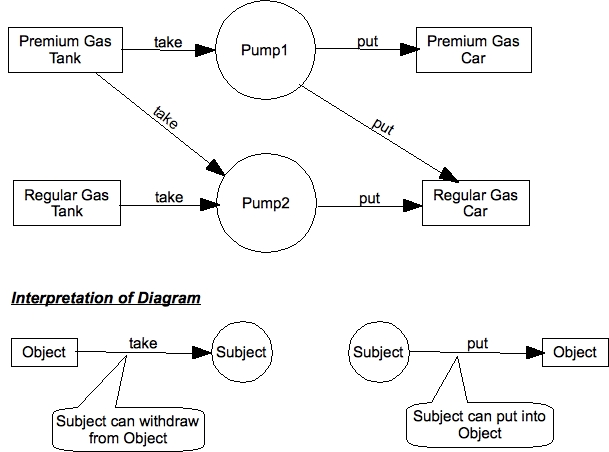
\includegraphics[width=0.6\linewidth]{Figures/gasSolution}  
  \caption{Access Diagram for Gas}
  \label{fig:access-diagram}
\end{figure}

Consider the following scenario. There are two grades of gas: \emph{P}
for premium gas and \emph{R} for regular gas.  There are two pumps:
\emph{Pump1} and \emph{Pump2}. There are two cars: a car that uses regular
gas (\emph{RGC}) and a car that requires premium gas (\emph{PGC}).

We assume the typical relation on gas grades: premium gas is higher
quality than regular gas, i.e., $R \leq_i P$. We also assume cars
specified as taking a particular grade of gas can safely take that
grade of gas or higher. In our example, \emph{RGC} can be fueled with
regular (R) gas or premium (P) gas, whereas \emph{PGC} can only be
fueled with premium (P) gas.

Figure~\ref{fig:access-diagram} diagrams the subjects, objects, and
types of access permitted in this scenario. Informally, subjects
\emph{act} on objects. The subjects in the scenario are \emph{Pump1}
and \emph{Pump2}.  The objects are the Premium Gas Tank \emph{(PGT)},
the Regular Gas Tank \emph{(RGT)}, the Premium Gas Car \emph{(PGC)}, and
the Regular Gas Car \emph{(RGC)}. What the diagram shows is that
\emph{Pump1} can only take or pump premium gas.  It can put gas into
both the regular and premium gas cars.  \emph{Pump2} can take or draw
from both premium and regular gas tanks, but it can only put gas into
the regular gas car.

\begin{table}[t]
  \centering
\begin{tabular}[h]{r | c}
  \emph{Subjects and Objects} & \emph{Integrity Level}\\
  \hline
  Premium Gas Tank \emph{PGT} & P\\
  Regular Gas Tank \emph{RGT} & R\\
  Pump1  & P\\
  Pump2& R\\
  Premium Gas Car \emph{PGC} & P\\
  Regular Gas Car \emph{RGC} &R\\
\end{tabular}
  \caption{Integrity Level Assignments}
  \label{tab:int-level-assignments}
\end{table}

\begin{table}[t]
  \centering
  \begin{tabular}[h]{r | c c c c}
    \textbf{Subject} & \textbf{PGT (P)} & \textbf{RGT (R)} &
    \textbf{PGC (P)} &
    \textbf{RGC (R)}\\
    \hline
    \emph{Pump1 (P)} & take & - & put & put\\
    \emph{Pump2 (R)} & take & take & - & put\\
  \end{tabular}
  \caption{Access-Control Matrix}
  \label{tab:access-control-matrix}
\end{table}

If we use $P$ as the integrity level for premium grade and $R$ as the
integrity level for regular grade, the subjects and objects have the
integrity level assignments shown in
Table~\ref{tab:int-level-assignments}. These assignments combined with
the access privileges shown in Figure~\ref{fig:access-diagram} result
in the access-control matrix in
Table~\ref{tab:access-control-matrix}.

Under the assumption that the integrity levels are \emph{partially
  ordered}, i.e., $R \leq_i R$, $P \leq_i P$, and $R \leq_i P$, we see
that the assignment of access rights in
Table~\ref{tab:access-control-matrix} conforms with Biba's Strict
Integrity policy. No car, in this assignment of \emph{take} and
\emph{put} privileges, can be filled with gas of lesser quality than
it is specified to take.

Using the access-control logic, we can formally represent the
access-control policy as shown in Figure~\ref{fig:access-control-gas},
where each formula describes the conditions under which it is
permitted for Pump1 or Pump2 to exercise a take or put privilege on an
object.
\begin{figure}[t]
  \centering
  \begin{align*}
    \ilv{Pump1} \leq_i \ilv{PGT} &\implies Pump1 \controls \action{take,PGT}\\
    \ilv{PGC} \leq_i \ilv{Pump1} &\implies Pump1 \controls \action{put,PGC}\\
    \ilv{RGC} \leq_i \ilv{Pump1} &\implies Pump1 \controls \action{put,RGC}\\
    \ilv{Pump2} \leq_i \ilv{PGT} &\implies Pump2 \controls \action{take,PGT}\\
    \ilv{Pump2} \leq_i \ilv{RGT} &\implies Pump2 \controls \action{take,RGT}\\
    \ilv{RGC} \leq_i \ilv{Pump2} &\implies Pump2 \controls
    \action{put,RGC}
  \end{align*}
  
  \caption{Access-Control Policy for Pumping Gas}
\label{fig:access-control-gas}
\end{figure}



\begin{figure}[t]
  \centering
\begin{tabular}{r<{.} >{$}p{0.7\linewidth}<{$}p{0.3\linewidth}}
  1 & Pump1 \says \action{put,PGC} & request\\
  2 & \ilv{PGC} \leq_i \ilv{Pump1} \implies Pump1 \controls \action{put,
        PGC}& integrity policy\\
  3 & \ilv{PGC} =_i P & level assignment\\
  4 & \ilv{Pump1} =_i P& level assignment\\
  5 & \ilv{P} \leq_i \ilv{P} & Reflexivity of $\leq_i$\\
  6 & \ilv{PGC} \leq_i \ilv{Pump1} & 3, 4, 5 $\leq_i$ Subst\\
  7 & Pump1 \controls \action{put, PGC} & 2, 6 Modus Ponens\\
  8 &  \action{put, PGC} & 7, 1 Controls
\end{tabular}  
  \caption{Pump1 Proof}
  \label{fig:pump1-proof}
\end{figure}

As an illustration, consider a request by \emph{Pump1} to put gas into
the premium-gas car \emph{PGC}. This request is formally represented as
\begin{gather*}
  Pump1 \says \action{put, PGC}.
\end{gather*}
We wish to determine if we should honor the request, i.e., if we can
conclude $\action{put, PGC}$. The relevant access-policy statement
from Table~\ref{tab:access-control-matrix} is
\begin{gather*}
  \ilv{PGC} \leq_i \ilv{Pump1} \implies Pump1 \controls \action{put,
    PGC}.
\end{gather*}
From Table~\ref{tab:int-level-assignments} we get the integrity level
assignments of \emph{Pump1} and \emph{PGC}:
\begin{gather*}
  \ilv{PGC} =_i P \text{ and } \ilv{Pump1} =_i P.
\end{gather*}
The request with the policy and level assignment statements is enough
to prove a theorem or derived inference rule justifying letting
\emph{Pump1} put gas into \emph{PGC}.  The derived inference rule is
below. Its proof is shown in Figure~\ref{fig:pump1-proof}.
\begin{gather*}
  \irule
  {
    \begin{array}{c}
      Pump1 \says \action{put, PGC}\\
      \ilv{PGC} \leq_i \ilv{Pump1} \implies Pump1 \controls \action{put,
        PGC}\\
      \ilv{PGC} =_i P \qquad \ilv{Pump1} =_i P
    \end{array}
  } 
  {\action{put, PGC}} 
  {}.
\end{gather*}


% \chinbox{
%   \begin{itemize}
%   \item Pump1 request to put gas into PGC
%   \item Derived theorem/inference rule justifying request
%   \item Refer to proof in Figure~\ref{fig:pump1-proof}
%   \end{itemize}
% }

% \section{Structural Operational Semantics}
% \label{sec:struct-oper-semant}

% Structural operational semantics (SOS) deals with the \emph{behavior}
% of programs, \cite{Plotkin04} and \cite{Huttel10}. It uses mathematics
% to describe and reason about the behavior of programs. We will use SOS
% to describe and reason about the expected behavior of cloud services
% and hardware devices.

% Structural operational semantics is defined in terms of the
% \emph{syntax} or \emph{structure} of a language or program. The
% underlying behavioral definitions use mathematical \emph{induction} to
% relate values to programs or language expressions.

% As a tutorial example, we develop the structural operational semantics
% for a simple arithmetic expression language, \textbf{AExp}. First, we
% introduce the syntax of \textbf{AExp}. Second, we define the semantics
% of \textbf{AExp}.

% \subsection{Syntax of AExp}
% \label{sec:syntax-aexp}

% Our illustrative example is to define the structural operational
% semantics for simple arithmetic expressions described by the set of
% formulas \textbf{AExp}. \textbf{AExp} is built on the set of natural
% numbers, which we call \textbf{num}.
% \begin{align*}
%   num &= \set{0, 1, 2, 3, \cdots}\\
%   AExp &::= const\;num \ora plus \;AExp_1\; AExp_2 \ora minus\; AExp_1
%   \;AExp_2 \ora times \;AExp_1\; AExp_2
% \end{align*}

% From the abstract syntax rule for \textbf{AExp} formulas above, we see
% that AExp expressions have one of four forms. Arithmetic expressions
% as defined are either:
% \begin{enumerate}
% \item a constant, i.e., \emph{const} followed by a natural number
%   (\emph{num}),
% \item \emph{plus} followed by two AExp expressions,
% \item \emph{minus } followed by two by two AExp expressions, or
% \item \emph{times} followed by two expressions.
% \end{enumerate}

% Using the above rules, we can construct AExp expressions and see if a
% given expression is a well-formed AExp expression.  For example,
% $const\;5$ is an AExp expression, i.e., $const \;5 \in AExp$ because
% $5 \in num$.  The symbol $n \not\in AExp$ because $n \not\in num$,
% i.e., $n$ is not a natural number, and $n$ is not covered by any of
% the rules defining AExp.

% The expression $plus\;(times (const\;1)\;(minus
% (const\;5)(const\;2)))(const\;3)$ is an AExp expression by the
% following chain of reasoning.
% \begin{enumerate}
% \item $plus\;(times\;1\;(minus(const\;5)(const\;2)))(const\;3)$ is an
%   AExp expression if both $\\(times\;1\; (minus(const\;5) (const\;2)))$
%   and $const\;3$ are AExp expressions. 3 is a \emph{num} so $const\; 3$
%   is an AExp expression.
% \item $(times(const\;1)\;(minus(const\;5)(const\;2)))$ is an AExp
%   expression if $(const\;1)$ and $\\(minus(const\;5) (const\;2))$ are.  1
%   is a \emph{num} so it is an AExp expression.
% \item $(minus(const\;5)(const\;2))$ is an AExp expression as 5 and 2
%   are \emph{nums}.
% \end{enumerate}


% \subsection{Semantics of AExp}
% \label{sec:semantics-aexp}

% Given the definition of AExp, we define the value or \emph{semantics}
% of AExp expressions as follows.
% \begin{enumerate}
% \item Natural numbers evaluate to themselves. We represent this as the
%   \emph{Const} rule
%   \begin{gather*}
%     \irule{}{const\;v \rightarrow v}{Const}{\text{ where }v \in num}
%   \end{gather*}
% \item \emph{plus} expressions evaluate to the sum of their
%   components. We represent this by the \emph{Plus} rule as:
%   \begin{gather*}
%     \irule{a_1 \rightarrow v_1 \quad a_2 \rightarrow
%       v_2}{plus\;a_1\;a_2 \rightarrow v}{Plus}{\text{ where } v = v_1+v_2}
%   \end{gather*}
% \item \emph{minus} expressions evaluate to the difference of the
%   values of their components. The semantics of \emph{minus}
%   expressions is given by the \emph{Minus} rule as:
%   \begin{gather*}
%     \irule{a_1 \rightarrow v_1 \quad a_2 \rightarrow
%       v_2}{minus\;a_1\;a_2 \rightarrow v}{Minus}{\text{ where } v = v_1-v_2}
%   \end{gather*}
% \item \emph{times} expressions evaluate to the product of the values
%   of their components. The semantics of \emph{times} expressions is
%   given by the \emph{times} rule as:
%   \begin{gather*}
%     \irule{a_1 \rightarrow v_1 \quad a_2 \rightarrow
%       v_2}{times\;a_1\;a_2 \rightarrow v}{Times}{\text{ where } v =
%       v_1 \times v_2}
%   \end{gather*}
% \end{enumerate}

% \subsection{Example}
% \label{sec:example}

% \begin{figure}[t]
%   \centering
% \begin{tabular}{|r<{.} >{$}p{0.48\linewidth}<{$}p{0.12\linewidth}|}
%   \hline
%   1 & const\;1 \rightarrow 1 & Const\\
%   2 & const\;2 \rightarrow 2 & Const\\
%   3 & const\;3 \rightarrow 3 & Const\\
%   4 & plus(const\;2)(const\;3) \rightarrow 5 & 2, 3 Plus\\
%   5 & times(const\;1)(plus(const\;2)(const\;3)) \rightarrow 5 & 1, 4 Times\\
%   \hline
% \end{tabular}    
%   \caption{Proof of $times(const\;1)(plus(const\;2)(const\;3))\rightarrow 5$}
%   \label{fig:sos-proof}
% \end{figure}

% To illustrate the use of structural operational semantics, we prove:
% \begin{gather*}
%   times(const\;1)(plus(const\;2)(const\;3)) \rightarrow 5.
% \end{gather*}
% Figure~\ref{fig:sos-proof} is a line-by-line proof using the semantics
% rules. The first three lines of the proof state that $const\;n
% \rightarrow n$ for $n=1,2,$ and 3. The justification in all three
% cases is the \emph{Const} rule corresponding the the semantics of
% constants that are natural numbers. Line 4's conclusion that
% $plus(const\;2)(const\;3) \rightarrow 5$ uses the \emph{Plus} rule
% where the hypotheses are specialized to the cases in lines 2 and
% 3. Finally, line 5 $times(const\;1)(plus(const\;2)(const\;3))
% \rightarrow 5$ is justified based on the \emph{Times} rule applied to
% lines 1 and 4.

% The proof can also be represented as a \emph{tree} of inference rules,
% as shown below.
% \begin{gather*}
%   \irule
%   {
%     { \irule
%       {}
%       {const\;1 \rightarrow 1}
%       {Const}
%     } \qquad 
%   {\irule
%   {
%     {\irule
%      {}
%      {const\;2 \rightarrow 2}
%      {Const}}
%    \qquad
%     {\irule
%       {}
%       {const\;3 \rightarrow 3}
%       {Const}
%     }
%   }
%   {plus(const\;2)(const\;3) \rightarrow 5}
%   {Plus}}}
%   {times(const\;1)(plus(const\;2)(const\;3)) \rightarrow 5}
%   {Times}.
% \end{gather*}
% We read the proof from the top down. Using the \emph{Const} rule we
% establish $const\;1 \rightarrow 1, const\;2 \rightarrow 2,$ and
% $const\;3 \rightarrow 3$. From $const \;2 \rightarrow 2$ and $const\;3
% \rightarrow 3$ we can use the \emph{Plus} rule to prove
% $plus(const\;2)(const\;3) \rightarrow 5$. From $const\;1 \rightarrow
% 1$ and $plus(const\;2)(const\;3) \rightarrow 5$, we can use the
% \emph{Times} inference rule to prove
% $times(const\;1)(plus(const\;2)(const\;3)) \rightarrow 5$. Note well
% that all leaves (starting points) of the proof start with the
% \emph{Const} rule, i.e., the only rule that does not depend on any
% assumptions or hypotheses.%  Inference rules without assumptions or
% % hyptheses are \emph{axioms}.

\chapter{Access-Control Logic in HOL}
\label{cha:acl-in-hol}

The previous sections introduced the application of an access-control
logic and structural operational semantics to formally describe and
reason about security and behavior. While the proofs we presented were
straightforward and easily comprehended, the practical question of
\emph{how to assure and certify the proofs are correct} is important
to answer. Almost every design has enough details that make pencil and
paper proofs cumbersome to manage. People are human and even the best,
brightest, and most experienced people can and do make mistakes.

To address these concerns, we use the Higher-Order Logic (HOL) proof
checker, \cite{HOL}. HOL is used by verification engineers in much the
same way as spreadsheet programs are used by accountants. Logical
definitions are entered into HOL. These definitions extend existing
logical theories in HOL. Based on these definitions and existing
theories containing their own definitions and theorems, new theorems
are postulated as goals and verifiers attempt to prove the goals to be
true. If proved true, then the goals are considered to be theorems.

% HOL is built on top of the \emph{ML} (Meta-Language) functional
% programming language \cite{ML}. Users interact with HOL using ML. For
% example, inference rules in HOL are ML functions whose outputs are
% theorems.

What follows is not intended to be a tutorial on how to use HOL,
rather it is intended to show examples of how HOL is used to check our
results. HOL is extensively documented: HOL Tutorial
\cite{HOLTutorial}, HOL Description \cite{HOLDescription}, HOL Logic
\cite{HOLLogic}, and HOL Reference \cite{HOLReference}. The source
code for building the HOL system is freely available at
\textsf{http://hol.sourceforge.net/}.

Everything presented here is fully described in the appendices. All
the source code necessary for constructing the HOL theories and
inference rules is in
Appendix~\ref{cha:acl-source-files}. Pretty-printed listings of each
HOL theory in terms of its datatypes, definitions, and theorems are in
Appendix~\ref{cha:acl-hol-reports}. Descriptions of the HOL
implementation of 36 access-control logic inference rules are in
Appendix~\ref{cha:access-control-logic}. These descriptions include
the name, source file, type signature, synopsis, description, failure
conditions, application example, and implementation of each inference
rule.

% \section{Introduction to the HOL Theorem Prover}
% \label{sec:intr-hol-syst}

% \begin{table*}[t]
% \begin{center}
%   \begin{footnotesize}
%     \begin{tabular}{|l|l|l|l|} \hline
%       \multicolumn{4}{|c|}{ } \\
%       \multicolumn{4}{|c|}{\bf Terms of the HOL Logic} \\
%       \multicolumn{4}{|c|}{ } \\
%       {\it Kind of term} & {\it \HOL{} notation} & {\it Standard
%         notation} & {\it Description} \\ \hline
%       & & & \\
%       Truth & {\small\verb|T|} & $\top$ & {\it true}\\ \hline Falsity
%       & {\small\verb|F|} & $\bot$ & {\it false}\\ \hline Negation &
%       {\small\verb|~|}$t$ & $\neg t$ & {\it not}$\ t$\\ \hline
%       Disjunction & $t_1${\small\verb|\/|}$t_2$ & $t_1\vee t_2$ &
%       $t_1\ ${\it or}$\ t_2$ \\ \hline Conjunction &
%       $t_1${\small\verb|/\|}$t_2$ & $t_1\wedge t_2$ & $t_1\ ${\it
%         and}$\ t_2$ \\ \hline Implication &
%       $t_1${\small\verb|==>|}$t_2$ & $t_1\implies t_2$ & $t_1\ ${\it
%         implies}$\ t_2$ \\ \hline Equality &
%       $t_1${\small\verb|=|}$t_2$ & $t_1 = t_2$ & $t_1\ ${\it equals}$\
%       t_2$ \\ \hline $\forall$-quantification &
%       {\small\verb|!|}$x${\small\verb|.|}$t$ & $\uquant{x}t$ & {\it
%         for\ all\ }$x: t$ \\ \hline $\exists$-quantification &
%       {\small\verb|?|}$x${\small\verb|.|}$t$ & $\equant{x}\ t$ & {\it
%         for\ some\ }$x: t$ \\ \hline $\hilbert$-term &

%       {\small\verb|@|}$x${\small\verb|.|}$t$ & $\hquant{x}t$ & {\it
%         an}$\ x\ ${\it such\ that:}$\ t$ \\ \hline Conditional &
%       {\small\verb|if|} $t$ {\small\verb|then|} $t_1$
%       {\small\verb|else|} $t_2$ & $(t\rightarrow t_1, t_2)$ & {\it if\
%       }$t${\it \ then\ }$t_1${\it\ else\ }$t_2$ \\ \hline
%     \end{tabular}
%   \end{footnotesize}
% \end{center}
%   \caption{Notation in HOL Proof Checker}
%   \label{tab:hol-notation}
% \end{table*}

% The HOL (higher-order logic) system is a collection of functional
% programs written in the functional programming language ML
% (meta-language) and executed by ML interpreters such as Moscow ML and
% PolyML. While it is infeasible to give a complete description of how
% to use HOL and implement the access-control logic within HOL, we give
% enough detail to give a qualitative understanding of what HOL does,
% how the logic is implemented as a conservative extension of the logic,
% and some examples.

% HOL is used in two modes: compiled or interactive.  HOL is used in a
% batch mode to compile pre-existing and previously verified theories
% efficiently and quickly. Users do not interact with HOL in this
% mode. Typically, all that is done is to execute \texttt{Holmake} on a
% command line in the appropriate subdirectory.

% HOL is used interactively to explore existing theories and to build
% new theories.  In interactive mode users work with the HOL interpreter
% using ML.  An example appears below.

% \begin{footnotesize}
%   \begin{session}
% \begin{verbatim}
% - BOOL_CASES_AX;
% > val it = |- !t. (t <=> T) \/ (t <=> F) : thm
% \end{verbatim}
%   \end{session}

% \end{footnotesize}
% The user prompt is ``\texttt{-}''. The user input is
% ``\texttt{BOOL\_CASES\_AX}'' terminated by ``\texttt{;}''.  HOL's
% response is after ``\texttt{>}''.

% \texttt{BOOL\_CASES\_AX} is the name of a theorem in HOL. The value
% associated with \texttt{BOOL\_CASES\_AX} is a \emph{theorem}, i.e., a
% value of type ``\texttt{thm}''). The theorem itself, using
% Table~\ref{tab:hol-notation} (taken from \cite{HOL}) to translate HOL
% notation into standard notation, is
% \begin{gather*}
%   \HOLTokenTurnstile{}
%   \HOLTokenForall{}\HOLBoundVar{t}. (\HOLBoundVar{t} \HOLTokenEquiv{}
%   T) \HOLTokenDisj{} (\HOLBoundVar{t} \HOLTokenEquiv{} F).
% \end{gather*}
% We recognize this theorem as stating that for all Boolean terms $t$,
% $t$ is either true or false.

% Theorems in HOL are \emph{sequents}, i.e., expressions of the form
% $\Gamma \vdash \Sigma$. A theorem consists of a (possibly empty) set
% of assumptions $\Gamma$ separated by the turnstile symbol $\vdash$ from
% the conclusion $\Sigma$. A theorem asserts that whenever all the terms
% in set $\Gamma$ are true, then the conclusion $\Sigma$ is guaranteed
% to be true as well.

% \begin{figure}[t]
%   \begin{center}
%     \begin{footnotesize}
%       \begin{gather*}
%         \irule{}{t \vdash t}{ASSUME t} \qquad
%         \irule{A_1 \vdash t_1 \implies t_2 \quad A_2 \vdash t_1}{A_1 \cup A_2 \vdash t_2}{MP}\qquad
%         \irule{\set{H_1, \cdots, H_n} \vdash t}{\vdash H_1 \implies
%           \cdots \implies H_n \implies t}{DISCH\_ALL}
%       \end{gather*}
%     \end{footnotesize}
%   \end{center}

%   \caption{Example HOL Inference Rules}
%   \label{fig:hol-inf-rules}
% \end{figure}

% Inference rules in HOL are functions that return values of type
% \texttt{thm} when applied to their
% arguments. Figure~\ref{fig:hol-inf-rules} describes three HOL
% inference rules, \texttt{\textit{ASSUME t, MP,}} and
% \texttt{\textit{DISCH\_ALL}}. The rule \texttt{\textit{ASSUME t}} says
% that if you assume Boolean term $t$, then you may conclude it as
% well. \texttt{\textit{MP}} corresponds to Modus Ponens: \emph{if p
%   then q, p, therefore q}. The rule \texttt{\textit{DISCH\_ALL}} moves
% all of the assumptions of a theorem into an implication ending in the
% conclusion.

% The example shown below in HOL shows the application of
% \texttt{ASSUME} twice followed by \texttt{MP} to conclude $q$ given $p
% \implies q$ and $p$. Note that terms in the HOL logic (as opposed to
% ML values and ML functions) are within backwards quotes
% \texttt{``-``}. ML functions and values are meta-logical; terms within
% backwards quotes are HOL objects.

% \begin{footnotesize}
%   \begin{session}
% \begin{verbatim}
% - val th1 = ASSUME ``p ==> q``;
% > val th1 =  [.] |- p ==> q : thm
% - val th2 = ASSUME ``p:bool``;
% > val th2 =  [.] |- p : thm
% - val th3 = MP th1 th2;
% > val th3 =  [..] |- q : thm
% - DISCH_ALL th3;
% > val it = |- (p ==> q) ==> p ==> q : thm
% \end{verbatim}
%   \end{session}

% \end{footnotesize}


% The inference rules in Figure~\ref{fig:hol-inf-rules} are low-level
% forward inference rules.  They are known as such because they take
% relatively small proof steps. HOL also has high-level decision
% procedures that take large steps.  For example, the function
% \texttt{PROVE} takes a list of theorems and attempts to prove the term
% to which it is applied. In the example below, \texttt{PROVE} is used
% to show that $x + 0 + y + z = y + (z + x)$ given a list of theorems on
% addition (associativity, symmetry, and identity).

% \begin{footnotesize}
%   \begin{session}
% \begin{verbatim}
% - ADD_ASSOC;
% > val it = 
%    |- !m n p. m + (n + p) = m + n + p : thm
% - ADD_SYM;
% > val it = |- !m n. m + n = n + m : thm
% - ADD_CLAUSES;
% > val it =
%     |- (0 + m = m) /\ (m + 0 = m) /\ 
%        (SUC m + n = SUC (m + n)) /\
%        (m + SUC n = SUC (m + n)) : thm
% - PROVE 
%    [ADD_ASSOC, ADD_SYM, ADD_CLAUSES] 
%    ``x+0+y+z = y+(z+x)``;
% > val it = |- x + 0 + y + z = y + (z + x) : thm
% \end{verbatim}
%   \end{session}

% \end{footnotesize}

% HOL is a rich system with many capabilities, particularly in the areas
% of defining new recursive types and structural induction. There are
% numerous theories ranging from mathematics (e.g., sets, relations, and
% real numbers) to applications such as the operational semantics of
% popular microprocessors such as the x-86 and ARM.  With the above as
% introduction, what follows is an overview of our implementation of
% structural operational semantics and the access-control logic in HOL.

% % \subsection{Structural Operational Semantics of Arithmetic
% %   Expressions}
% % \label{sec:struct-oper-semant-1}

% % % \chinbox{
% % %   \begin{itemize}
% % %   \item Define data type
% % %   \item Define rules
% % %   \item Prove example
% % %   \end{itemize}
% % % }
% % In this section we show how the structural operational semantics of
% % arithmetic expressions AExp is defined. As discussed before,
% % structural operational semantics is driven by the syntactic forms of
% % expressions. First, we define the syntax of AExp as a new
% % type. Second, we define the evaluation rules.

% % \paragraph{Defining the Syntax of AExp as a New Type}
% % \label{sec:defining-syntax-aexp}

% % Recall that the set of AExp expressions is defined using the natural
% % numbers \emph{num}, as shown below.
% % \begin{align*}
% %   num &= \set{0, 1, 2, 3, \cdots}\\
% %   AExp &::= const\;num \ora plus \;AExp_1\; AExp_2 \ora minus\; AExp_1
% %   \;AExp_2 \ora times \;AExp_1\; AExp_2
% % \end{align*}

% % In HOL, the natural numbers are built into the HOL system as the type
% % \emph{num}. Terms and their types have the form $term:type$, e.g.,
% % $1:num$ denotes that 1 is a natural number \emph{num}.

% % The function \texttt{HOL\_datatype} is used to define a
% % new type \texttt{AExp} in HOL.  The HOL session below shows the user
% % input. The \texttt{-} symbol at the start of the session is the HOL
% % prompt for user input. The user input starts with
% % \texttt{Hol\_datatype} and ends with the \texttt{;}. HOL's response is
% % shown in the last two lines indicating that HOL accepted the new type
% % definition.  

% % \setcounter{sessioncount}{0}
% % \begin{session}
% % \begin{verbatim}
% % - Hol_datatype `AExp = const of num
% %                   | plus of AExp => AExp
% %                   | minus of AExp => AExp
% %                   | times of AExp => AExp`;
% % <<HOL message: Defined type: "AExp">>
% % > val it = () : unit
% % \end{verbatim}
% % \end{session}

% % \paragraph{Defining the Semantics of AExp}
% % \label{sec:defin-semant-aexp}

% % % \begin{table}[t]
% % % \begin{center}
% % % \begin{tabular}{|l|l|l|l|} \hline
% % % \multicolumn{4}{|c|}{ } \\
% % % \multicolumn{4}{|c|}{\bf Terms of the HOL Logic} \\
% % % \multicolumn{4}{|c|}{ } \\
% % % {\it Kind of term} & {\it \HOL{} notation} &
% % % {\it Standard notation} &
% % % {\it Description} \\ \hline
% % %  & & & \\
% % % Truth & {\small\verb|T|} & $\top$ & {\it true}\\ \hline
% % % Falsity & {\small\verb|F|} & $\bot$ & {\it false}\\ \hline
% % % Negation & {\small\verb|~|}$t$ & $\neg t$ & {\it not}$\ t$\\ \hline
% % % Disjunction & $t_1${\small\verb|\/|}$t_2$ & $t_1\vee t_2$ &
% % % $t_1\ ${\it or}$\ t_2$ \\ \hline
% % % Conjunction & $t_1${\small\verb|/\|}$t_2$ & $t_1\wedge t_2$ &
% % % $t_1\ ${\it and}$\ t_2$ \\ \hline
% % % Implication & $t_1${\small\verb|==>|}$t_2$ & $t_1\implies t_2$ &
% % % $t_1\ ${\it implies}$\ t_2$ \\ \hline
% % % Equality & $t_1${\small\verb|=|}$t_2$ & $t_1 = t_2$ &
% % % $t_1\ ${\it equals}$\ t_2$ \\ \hline
% % % $\forall$-quantification & {\small\verb|!|}$x${\small\verb|.|}$t$ &
% % % $\uquant{x}t$ & {\it for\ all\ }$x: t$ \\ \hline
% % % $\exists$-quantification & {\small\verb|?|}$x${\small\verb|.|}$t$ &
% % % $\equant{x}\ t$ & {\it for\ some\ }$x: t$ \\ \hline
% % % $\hilbert$-term & {\small\verb|@|}$x${\small\verb|.|}$t$ &
% % % $\hquant{x}t$ & {\it an}$\ x\ ${\it such\ that:}$\ t$ \\ \hline
% % % Conditional & {\small\verb|if|} $t$ {\small\verb|then|} $t_1$
% % %               {\small\verb|else|} $t_2$ &
% % % $(t\rightarrow t_1, t_2)$ & {\it if\ }$t${\it \ then\ }$t_1${\it\ else\ }$t_2$
% % %  \\ \hline
% % % \end{tabular}
% % % \end{center}
% % %   \caption{Notation in HOL Proof Checker}
% % %   \label{tab:hol-notation}
% % % \end{table}

% % Recall that there are four rules defining the structural operational
% % semantics of AExp.
% % \begin{gather*}
% %   \irule{}{const\;v \rightarrow v}{Const}{\text{ where }v \in num} \\\\
% %   \irule{a_1 \rightarrow v_1 \quad a_2 \rightarrow
% %     v_2}{plus\;a_1\;a_2 \rightarrow v}{Plus}{\text{ where } v =
% %     v_1+v_2}\\\\
% %   \irule{a_1 \rightarrow v_1 \quad a_2 \rightarrow
% %     v_2}{minus\;a_1\;a_2 \rightarrow v}{Minus}{\text{ where } v =
% %     v_1-v_2}\\\\
% %     \irule{a_1 \rightarrow v_1 \quad a_2 \rightarrow
% %       v_2}{times\;a_1\;a_2 \rightarrow v}{Times}{\text{ where } v =
% %       v_1 \times v_2}
% % \end{gather*}

% % The above uses $\rightarrow$ as an \emph{infix} relation to symbolize
% % that an AExp expression evaluates to a value, e.g., $const\;2
% % \rightarrow 2$.  In HOL instead of an infix $\rightarrow$, we use a
% % \emph{prefix} relation $EV$, to relate AExp expressions to their
% % values, e.g., $EV\;(const\;2)\;2$.

% % Table~\ref{tab:hol-notation} shows the syntax used by the HOL system
% % to represent standard logical symbols.  The user interface to HOL uses
% % ASCII characters. Various combinations of ASCII characters are used to
% % represent standard logical symbols. For example, !x.t and ?x.t in HOL
% % represents $\forall x.t$ and $\exists x.t$ in standard
% % logic. Table~\ref{tab:hol-notation} will help  interpret the meaning
% % of what appears in the following HOL sessions below.

% % The \texttt{HOL\_reln} in HOL is used to define the structural
% % operational semantics of AExp expressions. As in previous HOL session,
% % the user prompt is ``\texttt{-}''; user input ends with
% % ``\texttt{;}''; HOL's response follows the ``\texttt{>}'' symbol. The
% % session below shows the rules defining the \texttt{EV} relation.
% % \begin{session}
% % \begin{verbatim}
% % - val (EV_rules,EV_ind,EV_cases) =
% %   Hol_reln
% %     `(!n:num. EV (const n) n) /\
% %      (!e:AExp e':AExp v:num v':num v'':num.
% %        (EV e v) /\ (EV e' v') /\ (v'' = v + v') ==>
% %        (EV (plus e e') v'')) /\
% %      (!e:AExp e':AExp v:num v':num v'':num.
% %        (EV e v) /\ (EV e' v') /\ (v'' = v - v') ==>
% %        (EV (minus e e') v'')) /\
% %      (!e:AExp e':AExp v:num v':num v'':num.
% %        (EV e v) /\ (EV e' v') /\ (v'' = v * v') ==>
% %        (EV (times e e') v''))`;
% % > val EV_rules =
% %     |- (!n. EV (const n) n) /\
% %        (!e e' v v' v''.
% %           EV e v /\ EV e' v' /\ (v'' = v + v') ==> 
% %           EV (plus e e') v'') /\
% %        (!e e' v v' v''.
% %           EV e v /\ EV e' v' /\ (v'' = v - v') ==> 
% %           EV (minus e e') v'') /\
% %        !e e' v v' v''.
% %          EV e v /\ EV e' v' /\ (v'' = v * v') ==> 
% %          EV (times e e') v'' : thm
% %     . . .
% % \end{verbatim}
% % \end{session}

% % The above session shows in part that \texttt{EV\_rules} is a
% % conjunction of the four universally quantified terms below
% % corresponding to \emph{Const, Plus, Minus,} and \emph{Times}. In
% % standard notation, \texttt{EV\_rules} is written as:
% % \begin{gather*}
% %   \vdash (\forall n:num. EV\;(const\;n)\;n) \wedge \\
% %   \quad (\forall (e:AExp)\:(e':AExp)\:(v:num)\:(v':num)\:(v'':num).\\
% %   \qquad (EV\;e\;v) \wedge (EV\;e'\;v') \wedge (v'' = v + v') \implies
% %   (EV\;(plus\;e\;e')\;v'')) \wedge\\
% %   \quad (\forall (e:AExp)\:(e':AExp)\:(v:num)\:(v':num)\:(v'':num).\\
% %   \qquad (EV\;e\;v) \wedge (EV\;e'\;v') \wedge (v'' = v - v') \implies
% %   (EV\;(minus\;e\;e')\;v'')) \wedge\\
% %   \quad (\forall (e:AExp)\:(e':AExp)\:(v:num)\:(v':num)\:(v'':num).\\
% %   \qquad (EV\;e\;v) \wedge (EV\;e'\;v') \wedge (v'' = v * v') \implies
% %   (EV\;(times\;e\;e')\;v'')).
% % \end{gather*}
% % Recall, theorems have the form $\Gamma \vdash t$, where $\Gamma$
% % denotes a \emph{list} of assumptions (hypotheses) and $t$ is the
% % \emph{conclusion}. In the case of \texttt{EV\_rules} the list of
% % assumptions $\Gamma$ is empty.

% % \texttt{HOL\_reln} in HOL also returns theorems corresponding to
% % induction and case analysis.  For brevity, we omit them here. The HOL
% % manuals \cite{HOLDescription}, \cite{HOLTutorial}, and
% % \cite{HOLReference} have full descriptions and examples of HOL
% % operators.

% % For convenience, we can break up the \texttt{EV\_rules} theorem into
% % its four conjuncts and give each one a name to the structural
% % operational semantics rule to which it corresponds.  This is shown
% % below.

% % \begin{session}
% % \begin{verbatim}
% % - val [Const,Plus,Minus,Times] = CONJUNCTS EV_rules;
% % > val Const = |- !n. EV (const n) n : thm
% %   val Plus =
% %     |- !e e' v v' v''.
% %          EV e v /\ EV e' v' /\ (v'' = v + v') ==> 
% %          EV (plus e e') v'' : thm
% %   val Minus =
% %     |- !e e' v v' v''.
% %          EV e v /\ EV e' v' /\ (v'' = v - v') ==> 
% %          EV (minus e e') v'' : thm
% %   val Times =
% %     |- !e e' v v' v''.
% %          EV e v /\ EV e' v' /\ (v'' = v * v') ==> 
% %          EV (times e e') v''
% % : thm
% % \end{verbatim}
% % \end{session}

% % \paragraph{Example Structural Operational Semantics Proof in HOL}
% % \label{sec:example-hol}

% % \begin{figure}[t]
% %   \centering
% %   \begin{tabular}{cc}
% %   \begin{minipage}{0.48\linewidth}
% %     \begin{tiny}
% % \begin{verbatim}
% % (***********************************************************
% % * DESCRIPTION
% % * constR ----------------
% % *         EV (const n) v
% % ***********************************************************)
% % fun constR v = SPEC v Const;

% % (***********************************************************
% % * DESCRIPTION
% % *        [.] |- EV aexp1 v   [..] |- EV aexp2 v'
% % * plusR ----------------------------------------- v+v'=v''
% % *          [...] |- EV (plus aexp1 aexp2) v''
% % ***********************************************************)
% % fun plusR th1 th2 =
% % let
% %   val th3 = CONV_RULE (TOP_DEPTH_CONV ANTE_CONJ_CONV) Plus
% %   val th4 = MATCH_MP th3 th1
% %   val th5 = MATCH_MP th4 th2
% %   val v1 = getAExpVal th1
% %   val v2 = getAExpVal th2
% % in
% %   MATCH_MP th5 (SYM(reduceLib.ADD_CONV ``^v1 + ^v2``))
% % end;
% % \end{verbatim}
% %     \end{tiny}
% %   \end{minipage}
% % &
% % \begin{minipage}{0.48\linewidth}
% %   \begin{tiny}
% % \begin{verbatim}
% % (***********************************************************
% % * DESCRIPTION
% % *         [.] |- EV aexp1 v   [..] |- EV aexp2 v'
% % * minusR ----------------------------------------- v-v'=v''
% % *           [...] |- EV (minus aexp1 aexp2) v''
% % ***********************************************************)
% % fun minusR th1 th2 =
% % let
% %   val th3 = CONV_RULE (TOP_DEPTH_CONV Conv.ANTE_CONJ_CONV) Minus
% %   val th4 = MATCH_MP th3 th1
% %   val th5 = MATCH_MP th4 th2
% %   val v1 = getAExpVal th1
% %   val v2 = getAExpVal th2
% % in
% %   MATCH_MP th5 (SYM(reduceLib.SBC_CONV ``^v1 - ^v2``))
% % end;

% % (***********************************************************
% % * DESCRIPTION
% % *         [.] |- EV aexp1 v   [..] |- EV aexp2 v'
% % * timesR ----------------------------------------- v*v'=v''
% % *           [...] |- EV (times aexp1 aexp2) v''
% % ***********************************************************)
% % fun timesR th1 th2 =
% % let
% %   val th3 = CONV_RULE (TOP_DEPTH_CONV Conv.ANTE_CONJ_CONV) Times
% %   val th4 = MATCH_MP th3 th1
% %   val th5 = MATCH_MP th4 th2
% %   val v1 = getAExpVal th1
% %   val v2 = getAExpVal th2
% % in
% %   MATCH_MP th5 (SYM(reduceLib.MUL_CONV ``^v1 * ^v2``))
% % end;

% % \end{verbatim}
% %   \end{tiny}
% % \end{minipage}
% % \end{tabular}
% %   \caption{HOL SOS Forward Inference Rules}
% %   \label{fig:hol-sos-rules}
% % \end{figure}

% % We reproduce the proof in Figure~\ref{fig:sos-proof} in the HOL
% % session below.  Within HOL we defined forward inference rules
% % \texttt{constR, plusR, minusR,} and \texttt{timesR} based on the
% % corresponding theorems \texttt{Const, Plus, Minus,} and
% % \texttt{Times}. Inference rules in HOL return objects of type
% % \texttt{thm} (theorems) when applied to their arguments. The inference
% % rules and their implementation in ML are shown in
% % Figure~\ref{fig:hol-sos-rules}. Each of the inference rules takes a
% % theorem about arithmetic expressions AExp and specializes it to the
% % arguments provided to the inference rule. In the case of
% % \texttt{constR}, the \texttt{SPEC} rule specializes $n$ to $v$ in the
% % \texttt{Const} theorem \HOLTokenTurnstile{}
% % \HOLTokenForall{}\HOLBoundVar{n}. EV (const \HOLBoundVar{n})
% % \HOLBoundVar{n}.

% % In the case of the \texttt{plusR} rule, the theorem
% % \HOLTokenTurnstile{} \HOLTokenForall{}\HOLBoundVar{e}
% % \HOLBoundVar{e\sp{\prime}} \HOLBoundVar{v} \HOLBoundVar{v\sp{\prime}}
% % \HOLBoundVar{v\sp{\prime\prime}}.  EV \HOLBoundVar{e} \HOLBoundVar{v}
% % \HOLTokenConj{} EV \HOLBoundVar{e\sp{\prime}}
% % \HOLBoundVar{v\sp{\prime}} \HOLTokenConj{}
% % (\HOLBoundVar{v\sp{\prime\prime}} = \HOLBoundVar{v} +
% % \HOLBoundVar{v\sp{\prime}}) \HOLTokenImp{} EV (plus \HOLBoundVar{e}
% % \HOLBoundVar{e\sp{\prime}}) \HOLBoundVar{v\sp{\prime\prime}}, the
% % theorem is first converted from the form $A \wedge B \implies C$ to
% % the equivalent form $A \implies (B \implies C)$. Then a form of modus
% % ponens is used that unifies what amounts to $A$ and $B$ to
% % \texttt{th1} and \texttt{th2}.  Finally, if \texttt{v'' = v + v'},
% % then the expected conclusion is reached.  The inference rules
% % \texttt{minusR} and \texttt{timesR} are similarly defined.

% % The terms \texttt{th1, th2, th3, th4,} and \texttt{th5} in the HOL
% % session below correspond to the five lines in
% % Figure~\ref{fig:sos-proof}. The HOL inference rule \texttt{constR}
% % applied to HOL term \texttt{``1``} produces the theorem \texttt{th1}
% % as shown below. Other theorems for constants 2 and 3 are introduced
% % using \texttt{constR} as well.  The \texttt{plusR} rule is used to
% % conclude 5 from the addition of constants 2 and 3.  This is theorem
% % \texttt{th4}. Finally, \texttt{th5} results from applying the
% % \texttt{timesR} inference rule to theorems \texttt{th1} and
% % \texttt{th4}.

% % \begin{session}
% % \begin{verbatim}
% % - val th1 = constR ``1``;
% % > val th1 = |- EV (const 1) 1 : thm
% % - val th2 = constR ``2``;
% % > val th2 = |- EV (const 2) 2 : thm
% % - val th3 = constR ``3``;
% % > val th3 = |- EV (const 3) 3 : thm
% % - val th4 = plusR th2 th3;
% % > val th4 = |- EV (plus (const 2) (const 3)) 5 : thm
% % - val th5 = timesR th1 th4;
% % > val th5 = |- EV (times (const 1) 
% %                   (plus (const 2) (const 3))) 5 : thm
% % -
% % \end{verbatim}
% % \end{session}


\section{Implementation of the Access-Control Logic in HOL}
\label{sec:access-control-logic-hol}

In this section we give a brief overview of the access-control logic
in HOL. We include as an illustration the gas station example
discussed earlier.

\paragraph{Defining the Syntax of the Access-Control Logic in HOL}
\label{sec:defining-syntax-hol}

We use \texttt{Hol\_datatype} to introduce the syntax of the
access-control logic into the HOL system.  The first three types of
expressions we introduce are \emph{principal} expressions
(\texttt{Princ}), \emph{integrity level} expressions
(\texttt{IntLevel}), and \emph{security level} expressions
(\texttt{SecLevel}). The actual HOL code is shown below.

HOL supports \emph{polymorphism}, i.e., the ability of expressions to
have the same form but accept values of different type.  For example,
\emph{lists} have the same structure. Either they are empty, or if
they are non-empty, then they all have a head element followed by the
rest of the list.  Lists are polymorphic in the sense that lists of
numbers, strings, bank accounts, tokens, etc., all have the same
structure, but can have different types of elements.

Polymorphism in HOL is accomplished by the use of \emph{type
  variables}. In HOL, type variables all start with a single quote
\texttt{'}. For example, the polymorphic variable \texttt{x:'a} in HOL
is a variable $x$ whose type is given by type variable
\texttt{'a}. When a specific type, e.g., \texttt{num} or
\texttt{bool}, is instantiated into \texttt{'a}, then all terms of
type \texttt{'a} will be instantiated with the same type.

Recall that there are three types of principal expressions:
\begin{align*}
P ::= A \ora P \with Q \ora P\quoting Q,
\end{align*}
where $A$ is the set of simple principal names, $P$ and $Q$ are
principal expressions, $P \with Q$ represents two principals together,
and $P \quoting Q$ is the compound principal $P$ quoting $Q$.

In HOL, we use the type constructor \texttt{Name} to construct
elements of type \texttt{Princ} from elements of type \texttt{'apn},
where \texttt{'apn} is a type variable that is instantiated to
specific types such as numbers, strings, lists, etc.

For example, if we wish to construct simple principal names out of
numbers we could write \texttt{Name 123456}, whose type would be
\texttt{num Princ}. We could use strings as principal names. For
example, \texttt{Name "Alice"} has type \texttt{string Princ}.  The
remaining operators in principal expressions closely correspond to
what is in \cite{ACST}.  \texttt{meet} and \texttt{quoting} in HOL
corresponds to $\with$ and $\quoting$ in \cite{ACST}.

In a similar fashion to principal names, we take advantage of
polymorphism and type variables for building integrity and security
levels, \texttt{IntLevel} and \texttt{SecLevel}.  For example, suppose
we have an integrity classification with two levels, \emph{Prem} for
premium and \emph{Reg} for regular. Suppose also that we have
previously defined these classification levels as the type
\emph{IClass}, i.e.,
\begin{gather*}
  IClass ::= Prem \ora Reg.
\end{gather*}

As there are many possible classification systems, we parameterized
both integrity and security levels in the access-control logic using
polymorphic type variables, in the case \texttt{'il} and
\texttt{'sl} for integrity and security levels, respectively. In the
case of integrity levels, we can have \texttt{iLab Prem} and
\texttt{iLab Reg} as integrity labels.

As simple principals are assigned integrity or security levels, we
need a way to map simple principals to integrity and security levels.
This is done with the functions \texttt{il} and \texttt{sl},
respectively.  For example, consider the case where simple principals
are constructed from strings, e.g., \texttt{Name "Alice"}. We refer
to Alice's integrity and security levels by \texttt{il (Name
  "Alice")} and \texttt{sl (Name "Alice")}, respectively.

The above examples show that the types \texttt{IntLevel} and
\texttt{SecLevel} are each parameterized by two type variables:
\begin{enumerate}
\item the underlying type of simple principal names: \texttt{'apn},
  (where \texttt{'apn} is thought of as an abbreviation for ``a
  principal name''), and
\item \texttt{'il} (or \texttt{'sl}) for the particular integrity
  (security) classification levels used, (where \texttt{'il} and
  \texttt{'sl} are thought of as abbreviations for ``integrity
  level'' and ``security level''), respectively.
\end{enumerate}

The following HOL session shows the definition in HOL of principal
expressions, integrity levels, and security levels.

\setcounter{sessioncount}{0}
\begin{session}
\begin{verbatim}
val _ = Hol_datatype 
    `Princ = Name of 'apn
           | meet of Princ => Princ
           | quoting of Princ => Princ;

     IntLevel = iLab of 'il
              | il of 'apn;

     SecLevel = sLab of 'sl
              | sl of 'apn`;
\end{verbatim}
\end{session}

We can now define the abstract syntax of formulas (\texttt{Form}) in
the access-control logic. The components of access-control logic
formulas in HOL closely corresponds to the syntax introduced in
\cite{ACST} with a few differences due to how new types are introduced
in HOL.
\begin{enumerate}
\item \texttt{TT} and \texttt{FF} represent \emph{true} and \emph{false}
\item \texttt{prop 'aavar} represents \emph{primitive propositions}
  parameterized by type variable \texttt{:'aavar} (note: we chose the
  name \texttt{'aavar} to ensure it appears first in the alphabetized
  list of type variables that parameterized formulas
  \texttt{Form}). For example, primitive propositions could be
  constructed from natural numbers (\texttt{:num})---\texttt{prop 123};
  or propositions could be constructed from strings
  (\texttt{:string})---\texttt{prop "read file"}.
\item Logical negation, conjunction, disjunction, implication, and
  equivalence are represented by \texttt{notf, andf, orf, impf}, and
  \texttt{eqf}.
\item The access-control logic operators $\says, \speaksfor,
  \controls$, and $\reps {P}{Q}{\varphi}$ are represented by
  \texttt{says, speaks\_for, controls}, and \texttt{reps} in HOL.
\item For comparing and assigning integrity and security levels we use
  the following: $il_1 \leq_i il_2$ is given by \texttt{il2 domi il1}
  (note the change in operand order), and $il_1 =_i il_2$ is given by
  \texttt{il1 eqi il2} in HOL. We pronounce \texttt{il2 domi il1} as
  ``$il_2$ \emph{dominates} $il_1$.'' We have similar syntax for security
  levels.
\item Finally, we have equality, partial, and total order relations on
  natural numbers: $n_1 = n_2, n_1 \leq n_2$ and $n_1 < n_2$. These
  are represented in HOL by \texttt{eqn, lte}, and \texttt{lt}.
\end{enumerate}

The function \texttt{Hol\_datatype} is used to define the syntax of
access-control logic formulas as a new type in HOL, as shown below.
\begin{session}
\begin{verbatim}
val _ = Hol_datatype
    `Form = TT
          | FF
          | prop of 'aavar
          | notf of Form
          | andf of Form => Form
          | orf of Form => Form
          | impf of Form => Form
          | eqf of Form => Form
          | says of 'apn Princ => Form
          | speaks_for of 'apn Princ => 'apn Princ
          | controls of 'apn Princ => Form
	  | reps of 'apn Princ => 'apn Princ => Form
	  | domi of ('apn, 'il) IntLevel => ('apn, 'il) IntLevel
	  | eqi of ('apn, 'il) IntLevel => ('apn, 'il) IntLevel
	  | doms of ('apn, 'sl) SecLevel => ('apn, 'sl) SecLevel
	  | eqs of ('apn, 'sl) SecLevel => ('apn, 'sl) SecLevel
	  | eqn of num => num
	  | lte of num => num
	  | lt of num => num`;
\end{verbatim}
\end{session}

The definitions of \texttt{Princ} and \texttt{Form} define
\emph{prefix} operators.  These operators are converted to their
\emph{infix} form (with precedence information) by the following
series of commands. Note that the number following \texttt{Infixr}
sets the precedence of the operator.  Higher numbers indicate greater
precedence.

\begin{session}
\begin{verbatim}
(* Change "meet" and "quoting" to infix operators *)

val _ = set_fixity "meet" (Infixr 630);
val _ = set_fixity "quoting" (Infixr 620);

(* and the rest *)

val _ = set_fixity "andf" (Infixr 580);
val _ = set_fixity "orf" (Infixr 570);
val _ = set_fixity "impf" (Infixr 560);
val _ = set_fixity "eqf" (Infixr 550);
val _ = set_fixity "says" (Infixr 590);
val _ = set_fixity "speaks_for" (Infixr 615);
val _ = set_fixity "controls" (Infixr 590);
val _ = set_fixity "domi" (Infixr 590);
val _ = set_fixity "eqi" (Infixr 590);
val _ = set_fixity "doms" (Infixr 590);
val _ = set_fixity "eqs" (Infixr 590);
val _ = set_fixity "eqn" (Infixr 590);
val _ = set_fixity "lte" (Infixr 590);
val _ = set_fixity "lt" (Infixr 590);
\end{verbatim}
\end{session}

\paragraph{Defining the Semantics of the Access-Control Logic in HOL}
\label{sec:defin-semant-access}

%%%% From HOL aclfoundationScript.sml ********************
% (** ACCESS CONTROL LOGIC FOUNDATION in our textbook *)
% (************************ 
% * ACCESS CONTROL LOGIC FOUNDATION in our textbook
% * The semantics of the logic is mainly built using Kripke structures.
% * Sets Li, Ls of integrity and security labels (or levels)  are
% * considered part of the syntax, and their partial orders Oi, Os are
% * separate parameters of the semantics and of the derivation system.
% * The components of the 
% * Kripke structure <W, I, J, imap, smap>
% * we use are:
% * (1) W, a non-empty set of worlds,
% * (2) I, an interpretation function mapping primitive propositions to the
% *     sets of worlds where the propositions are true,
% * (3) J, a function mapping principal expressions to relations on worlds,
% * (4) imap, a function mapping each simple principal name
% *     to an integrity level, and
% * (5) smap, a function mapping each simple principal name
% *     to a security level.
% * **********************)

% (***********************
% * HOL IMPLEMENTATION APPROACH
% * We introduce a Hol type Kripke that is parameterized on 
% * a non-empty set of worlds of arbitrary type, a set of integrity
% * levels of arbitrary type, and a set of security levels of arbitrary
% * type. At the end of this theory, we define Kripke as follows:
% * val _ = Hol_datatype 
% *    `Kripke = KS of ('var -> ('world set)) =>
% *                    ('pn -> ('world -> ('world set))) =>
% *                    ('pn -> 'il) =>
% *                    ('pn -> 'sl)`
% * where:
% * (1) 'world is a type variable for the type of possible worlds (note
% *      that every type in Hol is non-empty),
% * (2) 'var is a type variable for propositional variables,
% * (3) 'pn a type variable for the type of simple principal names,
% * (4) 'il is a type variable for the type of integrity levels, and
% * (5) 'sl is a type variable for the type of security levels,
% * 
% * To accomplish the above we do the following in order:
% * (1) define the type of partial orders, po
% * (2) define the type of principal expressions, Princ
% * (3) define the type of integrity level expressions, IntLevel,
% * (4) define the type of security level expressions, SecLevel,
% * (5) define the type of formulas, Form, and
% * (6) define the type of Kripke structures, Kripke.
% *************************)

In \cite{ACST}, the access-control logic semantics is defined using
Kripke structures. The core Kripke structure consists of a non-empty
set of worlds $W$, an interpretation function $I$ mapping each
primitive proposition to a set of worlds where the proposition is
true, and a function $J$ mapping principal expressions to a relation
on worlds. In \cite{ACST}, this core Kripke structure is a three-tuple
\krip{W,I,J}.

As many applications use either integrity levels, security levels, or
both, the core Kripke structure is extended by two functions $imap$
and $smap$, which map simple principal names to integrity and security
levels, respectively. The extended Kripke structure in \cite{ACST} is
the five-tuple \krip{W,I,J,imap,smap}.

There are many possible Kripke structures, not the least of which
differ in the sets of worlds $W$, interpretation functions $I$, and
mapping functions $J$, $imap$, and $smap$. In HOL we introduce a new
type called \texttt{Kripke}, which is parameterized by the following
type variables:
\begin{itemize}
\item a non-empty set of worlds of arbitrary type, in HOL this is the
  type variable \texttt{'aaworld},
\item a non-empty set of primitive propositions of arbitrary type
  \texttt{'aavar},
\item a non-empty set of simple principal names \texttt{'apn},
\item a set of integrity levels of arbitrary type \texttt{'il}, and
\item a set of security levels of arbitrary type \texttt{'sl}.
\end{itemize}

In HOL, the type \texttt{Kripke} is created by type constructor
\texttt{KS} applied to three functions in the following order:
\begin{enumerate}
\item the interpretation function $I$, whose type signature is
  \texttt{'aavar -> 'aaworld set},
\item the mapping $J$ from principals to a relation on worlds, whose
  type signature is \texttt{'apn -> ('aaworld -> ('aaworld set))},
\item the mapping function $imap$ from simple principal names to
  integrity levels, whose type signature is \texttt{'apn -> 'il}, and
\item the mapping function $smap$ from simple principal names to
  security levels, whose type signature is \texttt{'apn -> 'sl}.
\end{enumerate}
In HOL, the Kripke structures are built by expressions of the form:
$\mathtt{KS\; I\; J\; imap\; smap}$. The universe of worlds $W$ is
omitted because $W$ is included in the type signatures of $I$ and $J$.

The actual HOL code that defines type \texttt{Kripke} in HOL is below.
\begin{session}
\begin{verbatim}
val _ = Hol_datatype 
    `Kripke = KS of ('aavar -> ('aaworld set)) =>
    	      	    ('apn -> ('aaworld -> ('aaworld set))) =>
		    ('apn -> 'il) => ('apn -> 'sl)`;
\end{verbatim}
\end{session}

Once type \texttt{Kripke} is defined, we define accessor functions to retrieve the various components of Kripke structures.
\begin{align*}
  intpKS(KS\; \mathit{Intp}\; \mathit{Jfn}\; ilmap\; slmap) &= \mathit{Intp}\\
  jKS(KS\; \mathit{Intp}\; \mathit{Jfn}\; ilmap\; slmap) &=
  \mathit{Jfn}\\
  imapKS(KS\; \mathit{Intp}\; \mathit{Jfn}\; ilmap\; slmap) &= ilmap\\
  smapKS(KS\; \mathit{Intp}\; \mathit{Jfn}\; ilmap\; slmap) &= slmap.
\end{align*}
The definitions of the accessor functions in HOL are as follows.
\begin{session}
\begin{verbatim}
val intpKS_def =
    Define `intpKS(KS Intp Jfn ilmap slmap) = Intp`;

val jKS_def =
    Define `jKS(KS Intp Jfn ilmap slmap) = Jfn`;

val imapKS_def =
    Define `imapKS(KS Intp Jfn ilmap slmap) = ilmap`;

val smapKS_def =
    Define `smapKS(KS Intp Jfn ilmap slmap) = slmap`;
\end{verbatim}
\end{session}

With the above definitions it is straightforward to prove for any
Kripke structure $M$ deconstructed using the accessor functions, $M$
can be reassembled using \texttt{KS}, i.e.,
\begin{center}
\HOLTokenTurnstile{} \HOLTokenForall{}\HOLBoundVar{M}. \HOLBoundVar{M}
= KS (intpKS \HOLBoundVar{M}) (jKS \HOLBoundVar{M}) (imapKS
\HOLBoundVar{M}) (smapKS \HOLBoundVar{M}).
\end{center}

With the definitions of Kripke structures and the syntax of principal
expressions and formulas defined in HOL, we can define the semantics
of formulas in HOL corresponding to Figure~\ref{fig:semantics}.

\subparagraph{Extended mapping from principal expressions to relations
  on worlds}

The mapping function \texttt{J} to which \texttt{KS} is applied maps
\emph{simple principal names} to relations on worlds \texttt{'aaworld
  -> ('aaworld set)}. Note: the type of \texttt{J} differs slightly
from the definition of $J$ in \cite{ACST}. In particular, the type of
$J$ in \cite{ACST} is a function from principal names to the set
$\pow{W \times W}$. Here, the type of \texttt{J} is\texttt{ PName
  -> 'aaworld -> ('aaworld set)}.  This type is a bit more convenient
than the type of $J$ to fetch the set of worlds to which any
particular world is related.

Recall, the \emph{extended} mapping function $\hat{J}$ extends $J$ to
compound principal as shown below.
\begin{align*}
  \hat{J}(A) &= J, \text{ where A is a simple principal},\\
  \hat{J}(P \with Q) &= \hat{J}(P) \cup \hat{J}(Q), \text{ and}\\
  \hat{J}(P \quoting Q) &= \hat{J}(P) \circ \hat{J}(Q).
\end{align*}

The definition in HOL is shown below.
\begin{session}
\begin{verbatim}
val Jext_def =
    Define
    `(Jext (J:'pn -> 'w ->'w set) (Name s) = J s) /\
     (Jext J (P1 meet P2) = ((Jext J P1) RUNION (Jext J P2))) /\
     (Jext J (P1 quoting P2) = (Jext J P2) O (Jext J P1))`;
\end{verbatim}
\end{session}

\subparagraph{Defining Integrity and Security Levels and Partial
  Orders}

Introducing integrity and security levels into the HOL implementation
of the access-control logic comes next. We define two functions
\texttt{Lifn} and \texttt{Lsfn} that map integrity and security labels
to levels, and map simple principal names to levels. In the case of
integrity and security labels \texttt{iLab l} and \texttt{sLab l}, the
level returned is just \texttt{l}.  In the case of simple names, the
mapping of names to levels is specified by the \texttt{ilmap} and
\texttt{slmap} functions that are part of the Kripke structure $M$.
Specifically,
\begin{align*}
  ilmap &= imapKS \;M\\
  slmap &= smapKS \;M.
\end{align*}
The definition of \texttt{Lifn} and \texttt{Lsfn} are as follows:

\HOLTokenTurnstile{} (\HOLTokenForall{}\HOLBoundVar{M}
\HOLBoundVar{l}. Lifn \HOLBoundVar{M} (iLab \HOLBoundVar{l}) =
\HOLBoundVar{l}) \HOLTokenConj{}
\HOLTokenForall{}\HOLBoundVar{M} \HOLBoundVar{name}. Lifn \HOLBoundVar{M} (il \HOLBoundVar{name}) = imapKS \HOLBoundVar{M} \HOLBoundVar{name}

\HOLTokenTurnstile{} (\HOLTokenForall{}\HOLBoundVar{M}
\HOLBoundVar{l}. Lsfn \HOLBoundVar{M} (sLab \HOLBoundVar{l}) =
\HOLBoundVar{l}) \HOLTokenConj{} \HOLTokenForall{}\HOLBoundVar{M}
\HOLBoundVar{name}. Lsfn \HOLBoundVar{M} (sl \HOLBoundVar{name}) =
smapKS \HOLBoundVar{M} \HOLBoundVar{name}.

\noindent{}Their corresponding definitions in HOL are below. 
\begin{session}
\begin{verbatim}
val Lifn_def =
    Define
    `(Lifn M (iLab l) = l) /\
     (Lifn M (il name) = imapKS M name)`;
\end{verbatim}
\end{session}

\begin{session}
\begin{verbatim}
val Lsfn_def =
    Define
    `(Lsfn M (sLab l) = l) /\
     (Lsfn M (sl name) = smapKS M name)`;
\end{verbatim}
\end{session}

The Bell-LaPadula security model and Biba's Strict Integrity model use
a \emph{partial ordering} of integrity or security levels. In HOL,
partial orders are defined by \texttt{WeakOrder}. WeakOrder and its
components are defined below.

\HOLTokenTurnstile{} \HOLTokenForall{}\HOLBoundVar{Z}. WeakOrder
\HOLBoundVar{Z} \HOLTokenEquiv{} reflexive \HOLBoundVar{Z}
\HOLTokenConj{} antisymmetric \HOLBoundVar{Z} \HOLTokenConj{}
transitive \HOLBoundVar{Z}, where

\HOLTokenTurnstile{} \HOLTokenForall{}\HOLBoundVar{R}. reflexive
\HOLBoundVar{R} \HOLTokenEquiv{}
\HOLTokenForall{}\HOLBoundVar{x}. \HOLBoundVar{R} \HOLBoundVar{x}
\HOLBoundVar{x},

\HOLTokenTurnstile{} \HOLTokenForall{}\HOLBoundVar{R}. antisymmetric
\HOLBoundVar{R} \HOLTokenEquiv{} \HOLTokenForall{}\HOLBoundVar{x}
\HOLBoundVar{y}. \HOLBoundVar{R} \HOLBoundVar{x} \HOLBoundVar{y}
\HOLTokenConj{} \HOLBoundVar{R} \HOLBoundVar{y} \HOLBoundVar{x}
\HOLTokenImp{} (\HOLBoundVar{x} = \HOLBoundVar{y}), and

\HOLTokenTurnstile{} \HOLTokenForall{}\HOLBoundVar{R}. transitive
\HOLBoundVar{R} \HOLTokenEquiv{} \HOLTokenForall{}\HOLBoundVar{x}
\HOLBoundVar{y} \HOLBoundVar{z}. \HOLBoundVar{R} \HOLBoundVar{x}
\HOLBoundVar{y} \HOLTokenConj{} \HOLBoundVar{R} \HOLBoundVar{y}
\HOLBoundVar{z} \HOLTokenImp{} \HOLBoundVar{R} \HOLBoundVar{x}
\HOLBoundVar{z}.

We introduce a new type \texttt{po} (partial order) in HOL. The idea
is to have \texttt{po} be polymorphic like other types such as
\emph{lists}, e.g., \texttt{num list}---lists of natural numbers. If
$r$ is a partially ordered relation defined on a set of classification
labels defined in HOL as the type \texttt{class}, then we can
introduce the HOL type \texttt{class po}. To introduce the type
\texttt{'a po} in HOL is a three-step process.
\begin{enumerate}
\item The HOL predicate \texttt{WeakOrder} is used to select partial
  orderings from relations on type \texttt{'a}.
\item We prove a theorem stating that the new type \texttt{'a po} has
  at least one member.
\item We introduce the new type using \texttt{new\_type\_definition} in
  HOL using the theorem that states \texttt{'a po} is non-empty.
\end{enumerate}

The first step in HOL is to prove that there exists a relation on
\texttt{'a} that satisfies \texttt{WeakOrder}.  The HOL proof shown
below proves a theorem named EQ\_WeakOrder, which states equality (\$=
is the prefix form) is a partial order. The theorem and proof code in
HOL follow.

\HOLTokenTurnstile{} WeakOrder \$=
\begin{session}
\begin{verbatim}
val EQ_WeakOrder = 
    store_thm("EQ_WeakOrder",
	Term `WeakOrder ($=)`,
	REWRITE_TAC
	(map (SPEC ``($=):('a->'a->bool)``) 
	[(INST_TYPE [Type`:'g` |-> Type `:'a`] WeakOrder), 
	 reflexive_def, antisymmetric_def,transitive_def]) THEN
  	PROVE_TAC []);
\end{verbatim}
\end{session}

Using the EQ\_WeakOrder theorem we can prove easily that there exists
at least one relation satisfying WeakOrder.  The theorem and proof
code follow.

\HOLTokenTurnstile{} \HOLTokenExists{}\HOLBoundVar{R}. WeakOrder
\HOLBoundVar{R}
\begin{session}
\begin{verbatim}
val WeakOrder_Exists =
    save_thm
    ("WeakOrder_Exists",
     (EXISTS (Term `?R.WeakOrder R`, Term `$=`) EQ_WeakOrder));
\end{verbatim}
\end{session}

The theorem WeakOrder\_Exists is enough for HOL to conclude that the
type \texttt{:'a po} is non-empty. We introduce \texttt{po} as a new
type using \texttt{new_type_definition} as shown below.
\begin{session}
\begin{verbatim}
val po_type_definition = 
    new_type_definition ("po",WeakOrder_Exists);
\end{verbatim}
\end{session}
Executing the \texttt{new\_type\_definition} command introduces the following type definition:

\HOLTokenTurnstile{}
\HOLTokenExists{}\HOLBoundVar{rep}. TYPE_DEFINITION WeakOrder
\HOLBoundVar{rep}, where

\HOLTokenTurnstile{} TYPE_DEFINITION =\\\hspace*{0.3in}
(\HOLTokenLambda{}\HOLBoundVar{P} \HOLBoundVar{rep}.
(\HOLTokenForall{}\HOLBoundVar{x\sp{\prime}}
\HOLBoundVar{x\sp{\prime\prime}}. (\HOLBoundVar{rep}
\HOLBoundVar{x\sp{\prime}} = \HOLBoundVar{rep}
\HOLBoundVar{x\sp{\prime\prime}}) \HOLTokenImp{}
(\HOLBoundVar{x\sp{\prime}} = \HOLBoundVar{x\sp{\prime\prime}}))
\HOLTokenConj{} \HOLTokenForall{}\HOLBoundVar{x}. \HOLBoundVar{P}
\HOLBoundVar{x} \HOLTokenEquiv{}
\HOLTokenExists{}\HOLBoundVar{x\sp{\prime}}. \HOLBoundVar{x} =
\HOLBoundVar{rep} \HOLBoundVar{x\sp{\prime}})

The above type definition establishes the existence of the type
\texttt{'a po} constructed from relations of type \texttt{'a -> 'a ->
  bool}. Because the type \texttt{'a po} is non-empty, there is a
one-to-one mapping from elements of type \texttt{'a -> 'a -> bool} to
elements of type \texttt{'a po}. The HOL built-in function
\texttt{define\_new\_type\_bijections} produces the appropriate
theorems given the desired names of the abstraction and representation
functions (\texttt{PO} and \texttt{repPO}), and the name of the newly
defined type, here it is \texttt{po\_type\_definition}.

\begin{session}
\begin{verbatim}
val po_bij = save_thm ("po_bij",
     (define_new_type_bijections
      {name="po_tybij", ABS="PO", REP="repPO", 
       tyax=po_type_definition}));
\end{verbatim}
\end{session}

The resulting theorem po\_bij, is shown below.

\HOLTokenTurnstile{} (\HOLTokenForall{}(\HOLBoundVar{a} :'a po). PO
(repPO \HOLBoundVar{a}) = \HOLBoundVar{a})
\HOLTokenConj{}\\\hspace*{0.35in} \HOLTokenForall{}(\HOLBoundVar{r}
:'a \HOLTokenMap{} 'a \HOLTokenMap{} bool). WeakOrder \HOLBoundVar{r}
\HOLTokenEquiv{} (repPO (PO \HOLBoundVar{r}) =
\HOLBoundVar{r})\hfill{[po\_bij]}

The theorem po\_bij has two statements. (1) All elements $a:\mathtt{'a
  po}$ are mapped to their underlying representations by
$\mathtt{repPO\; a}$ and back again by $\mathtt{PO}$, and (2) for all
partial orders \texttt{r:'a -> 'a -> bool}, \texttt{PO} composed with
\texttt{repPO} is the identity function. Later on we will use both
\texttt{PO} and \texttt{repPO} to define partial orders using specific
integrity and security labels.

% \HOLTokenTurnstile{} (\HOLTokenForall{}\HOLBoundVar{a}. PO (repPO \HOLBoundVar{a}) = \HOLBoundVar{a}) \HOLTokenConj{} \HOLTokenForall{}\HOLBoundVar{r}. WeakOrder \HOLBoundVar{r} \HOLTokenEquiv{} (repPO (PO \HOLBoundVar{r}) = \HOLBoundVar{r})
% \HOLTokenTurnstile{} \HOLTokenForall{}\HOLBoundVar{r} \HOLBoundVar{r\sp{\prime}}. WeakOrder \HOLBoundVar{r} \HOLTokenImp{} WeakOrder \HOLBoundVar{r\sp{\prime}} \HOLTokenImp{} ((PO \HOLBoundVar{r} = PO \HOLBoundVar{r\sp{\prime}}) \HOLTokenEquiv{} (\HOLBoundVar{r} = \HOLBoundVar{r\sp{\prime}}))
% \begin{session}
% \begin{verbatim}
% val abs_po11 = 
%     save_thm
%     ("abs_po11",
%      (GEN_BETA_RULE (prove_abs_fn_one_one po_bij)));
% \end{verbatim}
% \end{session}

% \HOLTokenTurnstile{} \HOLTokenForall{}\HOLBoundVar{r}. WeakOrder \HOLBoundVar{r} \HOLTokenEquiv{} \HOLTokenExists{}\HOLBoundVar{a}. \HOLBoundVar{r} = repPO \HOLBoundVar{a}
% \begin{session}
% \begin{verbatim}
% val onto_po = 
%     save_thm
%     ("onto_po",
%      (prove_rep_fn_onto po_bij));
% \end{verbatim}
% \end{session}

% \HOLTokenTurnstile{} \HOLTokenForall{}\HOLBoundVar{a}. \HOLTokenExists{}\HOLBoundVar{r}. (\HOLBoundVar{a} = PO \HOLBoundVar{r}) \HOLTokenConj{} WeakOrder \HOLBoundVar{r}
% \begin{session}
% \begin{verbatim}
% val absPO_fn_onto = 
%     save_thm
%     ("absPO_fn_onto",
%      (prove_abs_fn_onto po_bij));
% \end{verbatim}
% \end{session}

% \HOLTokenTurnstile{} \HOLTokenForall{}\HOLBoundVar{a}. PO (repPO \HOLBoundVar{a}) = \HOLBoundVar{a}

% \HOLTokenTurnstile{} \HOLTokenForall{}\HOLBoundVar{r}. WeakOrder \HOLBoundVar{r} \HOLTokenEquiv{} (repPO (PO \HOLBoundVar{r}) = \HOLBoundVar{r})
% \begin{session}
% \begin{verbatim}
% val [PO_repPO, WO_repPO] = map2 (fn x => fn y => save_thm (x, y))
%                                 ["PO_repPO", "WO_repPO"]
%                                 (CONJUNCTS po_bij);
% \end{verbatim}
% \end{session}

% \HOLTokenTurnstile{} (\HOLTokenForall{}\HOLBoundVar{x}. repPO \HOLFreeVar{iPO} \HOLBoundVar{x} \HOLBoundVar{x}) \HOLTokenConj{}\\\hspace*{0.3in}
% (\HOLTokenForall{}\HOLBoundVar{x} \HOLBoundVar{y}. repPO \HOLFreeVar{iPO} \HOLBoundVar{x} \HOLBoundVar{y} \HOLTokenConj{} repPO \HOLFreeVar{iPO} \HOLBoundVar{y} \HOLBoundVar{x} \HOLTokenImp{} (\HOLBoundVar{x} = \HOLBoundVar{y})) \HOLTokenConj{}\\\hspace*{0.3in}
% \HOLTokenForall{}\HOLBoundVar{x} \HOLBoundVar{y}
% \HOLBoundVar{z}. repPO \HOLFreeVar{iPO} \HOLBoundVar{x}
% \HOLBoundVar{y} \HOLTokenConj{} repPO \HOLFreeVar{iPO} \HOLBoundVar{y}
% \HOLBoundVar{z} \HOLTokenImp{} repPO \HOLFreeVar{iPO} \HOLBoundVar{x}
% \HOLBoundVar{z}
% \begin{session}
% \begin{verbatim}
% val repPO_iPO_partial_order = save_thm ("repPO_iPO_partial_order",
%     REWRITE_RULE 
%     [(SPEC (Term`iPO:'a po`) PO_repPO),
%      WeakOrder, reflexive_def, transitive_def, antisymmetric_def] 
%     (SPEC (Term`(repPO iPO)`) WO_repPO));
% \end{verbatim}
% \end{session}

At this point, having defined Kripke structures, integrity and
security levels, and partial orders, we have all the necessary
components to define the semantics of access-control logic formulas.
The HOL session below shows the actual definition. Note that
\texttt{Oi:'il po} and \texttt{Os:'is po} are partial orderings on
integrity and security levels. \texttt{UNIV:('w)set} corresponds to W,
and is non-empty as every type in HOL is non-empty. Kripke structure\\
\texttt{M:('w,'v,'pn,'il,'is) Kripke} is parameterized by type
variables \texttt{'w} for worlds, \texttt{'v} for propositional
variables, \texttt{'pn} for simple principal names, \texttt{'il} for
integrity levels, and \texttt{'sl} for security levels.
\begin{session}
  \begin{tiny}
\begin{verbatim}
val Efn_def =
    Define
    `(Efn (Oi:'il po) (Os:'is po) (M:('w,'v,'pn,'il,'is) Kripke)
                  TT = UNIV) /\
     (Efn Oi Os M FF = {}) /\
     (Efn Oi Os M (prop p) = ((intpKS M) p)) /\
     (Efn Oi Os M (notf f) = (UNIV DIFF (Efn Oi Os M f))) /\
     (Efn Oi Os M (f1 andf f2) =
           ((Efn Oi Os M f1) INTER (Efn Oi Os M f2))) /\
     (Efn Oi Os M (f1 orf f2) =
           ((Efn Oi Os M f1) UNION (Efn Oi Os M f2))) /\
     (Efn Oi Os M (f1 impf f2) =
           ((UNIV DIFF (Efn Oi Os M f1)) UNION (Efn Oi Os M f2)))  /\
     (Efn Oi Os M (f1 eqf f2) =
           ((UNIV DIFF (Efn Oi Os M f1) UNION (Efn Oi Os M f2)) INTER
            (UNIV DIFF (Efn Oi Os M f2) UNION (Efn Oi Os M  f1)))) /\
     (Efn Oi Os M(P says f) =
           {w | Jext (jKS M) P w SUBSET (Efn Oi Os M f)}) /\
     (Efn Oi Os M (P speaks_for Q) =
           (if ((Jext (jKS M) Q) RSUBSET (Jext (jKS M) P)) then UNIV else
           {})) /\
     (Efn Oi Os M(P controls f) =
           ((UNIV DIFF
           ({w | Jext (jKS M) P w SUBSET Efn Oi Os M f})) UNION
            (Efn Oi Os M f)))  /\
     (Efn Oi Os M (reps P Q f) =
           ((UNIV DIFF
           ({w | Jext (jKS M) (P quoting Q) w SUBSET
                 Efn Oi Os M f})) UNION
            {w | Jext (jKS M) Q w SUBSET Efn Oi Os M f})) /\
     (Efn Oi Os M (intl1 domi intl2) = (* note inversion 3/12/09 *)
           (if repPO Oi (Lifn M intl2) (Lifn M intl1)
           then UNIV else {})) /\
     (Efn Oi Os M (intl2 eqi intl1) = (* ** note inversion 7/30/09 ** *)
           (if repPO Oi (Lifn M intl2) (Lifn M intl1)
           then UNIV else {}) INTER
           (if repPO Oi (Lifn M intl1) (Lifn M intl2)
           then UNIV else {})) /\
     (Efn Oi Os M (secl1 doms secl2) = (* note inversion *)
           (if repPO Os (Lsfn M secl2) (Lsfn M secl1)
           then UNIV else {})) /\
     (Efn Oi Os M (secl2 eqs secl1) = (* ** note inversion ** *)
           (if repPO Os (Lsfn M secl2) (Lsfn M secl1)
           then UNIV else {}) INTER
           (if repPO Os (Lsfn M secl1) (Lsfn M secl2)
           then UNIV else {})) /\
     (Efn Oi Os M ((numExp1:num) eqn (numExp2:num)) =
           (if (numExp1 = numExp2)
            then UNIV else {})) /\
     (Efn Oi Os M ((numExp1:num) lte (numExp2:num)) =
           (if (numExp1 <= numExp2)
            then UNIV else {})) /\
     (Efn Oi Os M ((numExp1:num) lt (numExp2:num)) =
           (if (numExp1 < numExp2)
            then UNIV else {}))`;
\end{verbatim}
  \end{tiny}
\end{session}

After defining the semantics as shown above, individual theorems corresponding to each operator or relation in the access-control logic are proved. Figure~\ref{fig:acl-hol-semantics} shows the collection of theorems that define the semantics of the access-control logic.
\begin{figure}[t]
  \centering
\begin{minipage}{1.0\linewidth}
\begin{small}
\HOLTokenTurnstile{} \HOLTokenForall{}\HOLBoundVar{Oi} \HOLBoundVar{Os} \HOLBoundVar{M}. Efn \HOLBoundVar{Oi} \HOLBoundVar{Os} \HOLBoundVar{M} TT = univ(:'v)\hfill{[TT\_def]}

\HOLTokenTurnstile{} \HOLTokenForall{}\HOLBoundVar{Oi} \HOLBoundVar{Os} \HOLBoundVar{M}. Efn \HOLBoundVar{Oi} \HOLBoundVar{Os} \HOLBoundVar{M} FF = \HOLTokenLeftbrace{}\HOLTokenRightbrace{} \hfill{[FF\_def]}

\HOLTokenTurnstile{} \HOLTokenForall{}\HOLBoundVar{Oi} \HOLBoundVar{Os} \HOLBoundVar{M} \HOLBoundVar{p}. Efn \HOLBoundVar{Oi} \HOLBoundVar{Os} \HOLBoundVar{M} (prop \HOLBoundVar{p}) = intpKS \HOLBoundVar{M} \HOLBoundVar{p} \hfill{[prop\_def]}

\HOLTokenTurnstile{} \HOLTokenForall{}\HOLBoundVar{Oi} \HOLBoundVar{Os} \HOLBoundVar{M} \HOLBoundVar{f}. Efn \HOLBoundVar{Oi} \HOLBoundVar{Os} \HOLBoundVar{M} (notf \HOLBoundVar{f}) = univ(:'v) DIFF Efn \HOLBoundVar{Oi} \HOLBoundVar{Os} \HOLBoundVar{M} \HOLBoundVar{f}\hfill{[notf\_def]}

\HOLTokenTurnstile{} \HOLTokenForall{}\HOLBoundVar{Oi} \HOLBoundVar{Os} \HOLBoundVar{M} \HOLBoundVar{f\sb{\mathrm{1}}} \HOLBoundVar{f\sb{\mathrm{2}}}.
     Efn \HOLBoundVar{Oi} \HOLBoundVar{Os} \HOLBoundVar{M} (\HOLBoundVar{f\sb{\mathrm{1}}} andf \HOLBoundVar{f\sb{\mathrm{2}}}) = Efn \HOLBoundVar{Oi} \HOLBoundVar{Os} \HOLBoundVar{M} \HOLBoundVar{f\sb{\mathrm{1}}} \HOLTokenInter{} Efn \HOLBoundVar{Oi} \HOLBoundVar{Os} \HOLBoundVar{M} \HOLBoundVar{f\sb{\mathrm{2}}} \hfill{[andf\_def]}

\HOLTokenTurnstile{} \HOLTokenForall{}\HOLBoundVar{Oi} \HOLBoundVar{Os} \HOLBoundVar{M} \HOLBoundVar{f\sb{\mathrm{1}}} \HOLBoundVar{f\sb{\mathrm{2}}}.
     Efn \HOLBoundVar{Oi} \HOLBoundVar{Os} \HOLBoundVar{M} (\HOLBoundVar{f\sb{\mathrm{1}}} orf \HOLBoundVar{f\sb{\mathrm{2}}}) = Efn \HOLBoundVar{Oi} \HOLBoundVar{Os} \HOLBoundVar{M} \HOLBoundVar{f\sb{\mathrm{1}}} \HOLTokenUnion{} Efn \HOLBoundVar{Oi} \HOLBoundVar{Os} \HOLBoundVar{M} \HOLBoundVar{f\sb{\mathrm{2}}} \hfill{[orf\_def]}

\HOLTokenTurnstile{} \HOLTokenForall{}\HOLBoundVar{Oi} \HOLBoundVar{Os} \HOLBoundVar{M} \HOLBoundVar{f\sb{\mathrm{1}}} \HOLBoundVar{f\sb{\mathrm{2}}}.
     Efn \HOLBoundVar{Oi} \HOLBoundVar{Os} \HOLBoundVar{M} (\HOLBoundVar{f\sb{\mathrm{1}}} impf \HOLBoundVar{f\sb{\mathrm{2}}}) = \hfill{[impf\_def]}\\\hspace*{0.3in}
     univ(:'v) DIFF Efn \HOLBoundVar{Oi} \HOLBoundVar{Os} \HOLBoundVar{M} \HOLBoundVar{f\sb{\mathrm{1}}} \HOLTokenUnion{} Efn \HOLBoundVar{Oi} \HOLBoundVar{Os} \HOLBoundVar{M} \HOLBoundVar{f\sb{\mathrm{2}}} 

\HOLTokenTurnstile{} \HOLTokenForall{}\HOLBoundVar{Oi} \HOLBoundVar{Os} \HOLBoundVar{M} \HOLBoundVar{f\sb{\mathrm{1}}} \HOLBoundVar{f\sb{\mathrm{2}}}.
     Efn \HOLBoundVar{Oi} \HOLBoundVar{Os} \HOLBoundVar{M} (\HOLBoundVar{f\sb{\mathrm{1}}} eqf \HOLBoundVar{f\sb{\mathrm{2}}}) = \hfill{[eqf\_def]}\\\hspace*{0.3in}
     (univ(:'v) DIFF Efn \HOLBoundVar{Oi} \HOLBoundVar{Os} \HOLBoundVar{M} \HOLBoundVar{f\sb{\mathrm{1}}} \HOLTokenUnion{} Efn \HOLBoundVar{Oi} \HOLBoundVar{Os} \HOLBoundVar{M} \HOLBoundVar{f\sb{\mathrm{2}}}) \HOLTokenInter{}\\\hspace*{0.3in}
     (univ(:'v) DIFF Efn \HOLBoundVar{Oi} \HOLBoundVar{Os} \HOLBoundVar{M} \HOLBoundVar{f\sb{\mathrm{2}}} \HOLTokenUnion{} Efn \HOLBoundVar{Oi} \HOLBoundVar{Os} \HOLBoundVar{M} \HOLBoundVar{f\sb{\mathrm{1}}})

\HOLTokenTurnstile{} \HOLTokenForall{}\HOLBoundVar{Oi} \HOLBoundVar{Os} \HOLBoundVar{M} \HOLBoundVar{P} \HOLBoundVar{f}.
     Efn \HOLBoundVar{Oi} \HOLBoundVar{Os} \HOLBoundVar{M} (\HOLBoundVar{P} says \HOLBoundVar{f}) = \hfill{[says\_def]}\\\hspace*{0.3in} \HOLTokenLeftbrace{}\HOLBoundVar{w} $\mid$ Jext (jKS \HOLBoundVar{M}) \HOLBoundVar{P} \HOLBoundVar{w} \HOLTokenSubset{} Efn \HOLBoundVar{Oi} \HOLBoundVar{Os} \HOLBoundVar{M} \HOLBoundVar{f}\HOLTokenRightbrace{}

\HOLTokenTurnstile{} \HOLTokenForall{}\HOLBoundVar{Oi} \HOLBoundVar{Os} \HOLBoundVar{M} \HOLBoundVar{P} \HOLBoundVar{Q}.
     Efn \HOLBoundVar{Oi} \HOLBoundVar{Os} \HOLBoundVar{M} (\HOLBoundVar{P} speaks_for \HOLBoundVar{Q}) = \hfill{[speaks\_for\_def]}\\\hspace*{0.3in}
\HOLKeyword{if} Jext (jKS \HOLBoundVar{M}) \HOLBoundVar{Q} RSUBSET Jext (jKS \HOLBoundVar{M}) \HOLBoundVar{P} \HOLKeyword{then} univ(:'v) \HOLKeyword{else} \HOLTokenLeftbrace{}\HOLTokenRightbrace{}

\HOLTokenTurnstile{} \HOLTokenForall{}\HOLBoundVar{Oi} \HOLBoundVar{Os} \HOLBoundVar{M} \HOLBoundVar{P} \HOLBoundVar{f}.
     Efn \HOLBoundVar{Oi} \HOLBoundVar{Os} \HOLBoundVar{M} (\HOLBoundVar{P} controls \HOLBoundVar{f}) = \hfill{[controls\_def]}\\\hspace*{0.3in}
     univ(:'v) DIFF \HOLTokenLeftbrace{}\HOLBoundVar{w} $\mid$ Jext (jKS \HOLBoundVar{M}) \HOLBoundVar{P} \HOLBoundVar{w} \HOLTokenSubset{} Efn \HOLBoundVar{Oi} \HOLBoundVar{Os} \HOLBoundVar{M} \HOLBoundVar{f}\HOLTokenRightbrace{} \HOLTokenUnion{}
     Efn \HOLBoundVar{Oi} \HOLBoundVar{Os} \HOLBoundVar{M} \HOLBoundVar{f}

\HOLTokenTurnstile{} \HOLTokenForall{}\HOLBoundVar{Oi} \HOLBoundVar{Os} \HOLBoundVar{M} \HOLBoundVar{P} \HOLBoundVar{Q} \HOLBoundVar{f}.
     Efn \HOLBoundVar{Oi} \HOLBoundVar{Os} \HOLBoundVar{M} (reps \HOLBoundVar{P} \HOLBoundVar{Q} \HOLBoundVar{f}) = \hfill{[reps\_def]}\\\hspace*{0.3in}
     univ(:'v) DIFF \HOLTokenLeftbrace{}\HOLBoundVar{w} $\mid$ Jext (jKS \HOLBoundVar{M}) (\HOLBoundVar{P} quoting \HOLBoundVar{Q}) \HOLBoundVar{w} \HOLTokenSubset{} Efn \HOLBoundVar{Oi} \HOLBoundVar{Os} \HOLBoundVar{M} \HOLBoundVar{f}\HOLTokenRightbrace{} \HOLTokenUnion{}\\\hspace*{0.3in}
     \HOLTokenLeftbrace{}\HOLBoundVar{w} $\mid$ Jext (jKS \HOLBoundVar{M}) \HOLBoundVar{Q} \HOLBoundVar{w} \HOLTokenSubset{} Efn \HOLBoundVar{Oi} \HOLBoundVar{Os} \HOLBoundVar{M} \HOLBoundVar{f}\HOLTokenRightbrace{}

\HOLTokenTurnstile{} \HOLTokenForall{}\HOLBoundVar{Oi} \HOLBoundVar{Os} \HOLBoundVar{M} \HOLBoundVar{intl\sb{\mathrm{1}}} \HOLBoundVar{intl\sb{\mathrm{2}}}.
     Efn \HOLBoundVar{Oi} \HOLBoundVar{Os} \HOLBoundVar{M} (\HOLBoundVar{intl\sb{\mathrm{1}}} domi \HOLBoundVar{intl\sb{\mathrm{2}}}) = \hfill{[domi\_def]}\\\hspace*{0.3in}
     \HOLKeyword{if} repPO \HOLBoundVar{Oi} (Lifn \HOLBoundVar{M} \HOLBoundVar{intl\sb{\mathrm{2}}}) (Lifn \HOLBoundVar{M} \HOLBoundVar{intl\sb{\mathrm{1}}}) \HOLKeyword{then} univ(:'v) \HOLKeyword{else} \HOLTokenLeftbrace{}\HOLTokenRightbrace{}

\HOLTokenTurnstile{} \HOLTokenForall{}\HOLBoundVar{Oi} \HOLBoundVar{Os} \HOLBoundVar{M} \HOLBoundVar{intl\sb{\mathrm{2}}} \HOLBoundVar{intl\sb{\mathrm{1}}}.
     Efn \HOLBoundVar{Oi} \HOLBoundVar{Os} \HOLBoundVar{M} (\HOLBoundVar{intl\sb{\mathrm{2}}} eqi \HOLBoundVar{intl\sb{\mathrm{1}}}) = \hfill{[eqi\_def]}\\\hspace*{0.3in}
     (\HOLKeyword{if} repPO \HOLBoundVar{Oi} (Lifn \HOLBoundVar{M} \HOLBoundVar{intl\sb{\mathrm{2}}}) (Lifn \HOLBoundVar{M} \HOLBoundVar{intl\sb{\mathrm{1}}}) \HOLKeyword{then}
        univ(:'v)
      \HOLKeyword{else}
        \HOLTokenLeftbrace{}\HOLTokenRightbrace{}) \HOLTokenInter{}\\\hspace*{0.3in}
     \HOLKeyword{if} repPO \HOLBoundVar{Oi} (Lifn \HOLBoundVar{M} \HOLBoundVar{intl\sb{\mathrm{1}}}) (Lifn \HOLBoundVar{M} \HOLBoundVar{intl\sb{\mathrm{2}}}) \HOLKeyword{then} univ(:'v) \HOLKeyword{else} \HOLTokenLeftbrace{}\HOLTokenRightbrace{}

\HOLTokenTurnstile{} \HOLTokenForall{}\HOLBoundVar{Oi} \HOLBoundVar{Os} \HOLBoundVar{M} \HOLBoundVar{secl\sb{\mathrm{1}}} \HOLBoundVar{secl\sb{\mathrm{2}}}.
     Efn \HOLBoundVar{Oi} \HOLBoundVar{Os} \HOLBoundVar{M} (\HOLBoundVar{secl\sb{\mathrm{1}}} doms \HOLBoundVar{secl\sb{\mathrm{2}}}) = \hfill{[doms\_def]}\\\hspace*{0.3in}
     \HOLKeyword{if} repPO \HOLBoundVar{Os} (Lsfn \HOLBoundVar{M} \HOLBoundVar{secl\sb{\mathrm{2}}}) (Lsfn \HOLBoundVar{M} \HOLBoundVar{secl\sb{\mathrm{1}}}) \HOLKeyword{then} univ(:'v) \HOLKeyword{else} \HOLTokenLeftbrace{}\HOLTokenRightbrace{}

\HOLTokenTurnstile{} \HOLTokenForall{}\HOLBoundVar{Oi} \HOLBoundVar{Os} \HOLBoundVar{M} \HOLBoundVar{secl\sb{\mathrm{2}}} \HOLBoundVar{secl\sb{\mathrm{1}}}.
     Efn \HOLBoundVar{Oi} \HOLBoundVar{Os} \HOLBoundVar{M} (\HOLBoundVar{secl\sb{\mathrm{2}}} eqs \HOLBoundVar{secl\sb{\mathrm{1}}}) = \hfill{[eqs\_def]}\\\hspace*{0.3in}
     (\HOLKeyword{if} repPO \HOLBoundVar{Os} (Lsfn \HOLBoundVar{M} \HOLBoundVar{secl\sb{\mathrm{2}}}) (Lsfn \HOLBoundVar{M} \HOLBoundVar{secl\sb{\mathrm{1}}}) \HOLKeyword{then}
        univ(:'v)
      \HOLKeyword{else}
        \HOLTokenLeftbrace{}\HOLTokenRightbrace{}) \HOLTokenInter{}\\\hspace*{0.3in}
     \HOLKeyword{if} repPO \HOLBoundVar{Os} (Lsfn \HOLBoundVar{M} \HOLBoundVar{secl\sb{\mathrm{1}}}) (Lsfn \HOLBoundVar{M} \HOLBoundVar{secl\sb{\mathrm{2}}}) \HOLKeyword{then} univ(:'v) \HOLKeyword{else} \HOLTokenLeftbrace{}\HOLTokenRightbrace{}

\HOLTokenTurnstile{} \HOLTokenForall{}\HOLBoundVar{Oi} \HOLBoundVar{Os} \HOLBoundVar{M} \HOLBoundVar{numExp\sb{\mathrm{1}}} \HOLBoundVar{numExp\sb{\mathrm{2}}}.
     Efn \HOLBoundVar{Oi} \HOLBoundVar{Os} \HOLBoundVar{M} (\HOLBoundVar{numExp\sb{\mathrm{1}}} eqn \HOLBoundVar{numExp\sb{\mathrm{2}}}) = \hfill{[eqn\_def]}\\\hspace*{0.3in}
     \HOLKeyword{if} \HOLBoundVar{numExp\sb{\mathrm{1}}} = \HOLBoundVar{numExp\sb{\mathrm{2}}} \HOLKeyword{then} univ(:'v) \HOLKeyword{else} \HOLTokenLeftbrace{}\HOLTokenRightbrace{}

\HOLTokenTurnstile{} \HOLTokenForall{}\HOLBoundVar{Oi} \HOLBoundVar{Os} \HOLBoundVar{M} \HOLBoundVar{numExp\sb{\mathrm{1}}} \HOLBoundVar{numExp\sb{\mathrm{2}}}.
     Efn \HOLBoundVar{Oi} \HOLBoundVar{Os} \HOLBoundVar{M} (\HOLBoundVar{numExp\sb{\mathrm{1}}} lte \HOLBoundVar{numExp\sb{\mathrm{2}}}) = \hfill{[lte\_def]}\\\hspace*{0.3in}
     \HOLKeyword{if} \HOLBoundVar{numExp\sb{\mathrm{1}}} \HOLTokenLeq{} \HOLBoundVar{numExp\sb{\mathrm{2}}} \HOLKeyword{then} univ(:'v) \HOLKeyword{else} \HOLTokenLeftbrace{}\HOLTokenRightbrace{}

\HOLTokenTurnstile{} \HOLTokenForall{}\HOLBoundVar{Oi} \HOLBoundVar{Os} \HOLBoundVar{M} \HOLBoundVar{numExp\sb{\mathrm{1}}} \HOLBoundVar{numExp\sb{\mathrm{2}}}.
     Efn \HOLBoundVar{Oi} \HOLBoundVar{Os} \HOLBoundVar{M} (\HOLBoundVar{numExp\sb{\mathrm{1}}} lt \HOLBoundVar{numExp\sb{\mathrm{2}}}) = \hfill{[lt\_def]}\\\hspace*{0.3in}
\HOLKeyword{if} \HOLBoundVar{numExp\sb{\mathrm{1}}} \HOLTokenLt{} \HOLBoundVar{numExp\sb{\mathrm{2}}} \HOLKeyword{then} univ(:'v) \HOLKeyword{else} \HOLTokenLeftbrace{}\HOLTokenRightbrace{}
\end{small}
\end{minipage}  
\caption{Theorems Defining Semantics of the Access-Control Logic}
\label{fig:acl-hol-semantics}
\end{figure}

\clearpage{}

\section{Access-Control Logic Inference Rules in HOL}
\label{sec:acl-inference-rules}

Our objective for embedding the access-control logic into HOL, as a
conservative extension of the HOL logic, is to provide sound
computer-assisted reasoning tools for access-control logic users. To
do this, we provide 36 inference rules, as shown in
Appendix~\ref{cha:access-control-logic}, which correspond closely to
the inference rules in the textbook \emph{Access Control, Security,
  and Trust: A Logical Approach}, \cite{ACST}.

Each inference rule is described in terms of its name, file containing
its definition, synopsis, description, failure conditions, an example
application, and its implementation. With few exceptions, inference
rules are small functional programs that specialize and unify of the
bound variables of relevant theorems.

\chapter{Integrity Example in HOL}
\label{cha:integrity-example}
We now turn to showing how the integrity example in
Section~\ref{sec:examples} involving premium and regular gas is
described and verified in HOL. Our first task is to define the
integrity levels themselves, how they are related, and show that the
relation is a partial order. The steps we take are the following:
\begin{enumerate}
\item Define the integrity levels, in this case \texttt{Reg} and
  \texttt{Prem}.
\item Define the relation \texttt{ICOrder } on integrity levels.
\item Prove that \texttt{ICOrder} is reflexive, antisymmetric, and
  transitive and thus satisfies the \texttt{WeakOrder} condition
  necessary for the type \texttt{(ICOrder) po}.
\end{enumerate}

\section{Introducing the Integrity Levels in HOL}
\begin{table}[t]
  \centering
  \begin{tabular}{cc|c}
    \textbf{y} & \textbf{x} & \textbf{ICOrder y x}\\
    \hline
    Reg & Reg & T\\
    Reg & Prem & T\\
    Prem & Reg & F\\
    Prem & Prem & T
  \end{tabular}
  \caption{Ordering on Integrity Levels}
  \label{tab:ICOrder}
\end{table}

We introduce the integrity levels \texttt{Prem} and \texttt{Reg} as a new datatype \texttt{IClass} in HOL.
\begin{session}
\begin{verbatim}
val _ = Hol_datatype
    `IClass = Prem | Reg`;
\end{verbatim}
\end{session}

Next, we define the ordering on \texttt{IClass} according to
Table~\ref{tab:ICOrder}. \texttt{Prem} dominates \texttt{Reg},
\texttt{Prem} dominates itself, and \texttt{Reg} dominates itself.
\begin{session}
\begin{verbatim}
val ICOrder_def = 
 Define `ICOrder y x = 
 if x = Prem then T else if y = Prem then F else T`;
\end{verbatim}
\end{session}

With the above definition we can build what amounts to Table~\ref{tab:ICOrder} in HOL as a list of theorems \texttt{ICO_table} as shown below.
\begin{session}
\begin{verbatim}
- val ICO_table = foldl (uncurry append) []
   (map (fn x => map (fn y =>
     REWRITE_CONV 
       [ICOrder_def, TypeBase.distinct_of (Type`:IClass`),
                     GSYM (TypeBase.distinct_of (Type`:IClass`))]
            (Term`ICOrder ^x ^y`))
            [``Prem``,``Reg``])
	    [``Prem``,``Reg``]);
> val ICO_table =
  [|- ICOrder Reg Prem <=> T, |- ICOrder Reg Reg <=> T,
   |- ICOrder Prem Prem <=> T, |- ICOrder Prem Reg <=> F] : thm list
\end{verbatim}
\end{session}

From the definition of \texttt{ICOrder} it is straightforward to see that it is a partial order, i.e., antisymmetric, reflexive, and transitive.

\HOLTokenTurnstile{} antisymmetric ICOrder \hfill{[ICOrder_antisymmetric]}

\HOLTokenTurnstile{} reflexive ICOrder \hfill{[ICOrder_reflexive]}

\HOLTokenTurnstile{} transitive ICOrder \hfill{[ICOrder_transitive]}

The following are short proofs in HOL that prove these three
properties.

\begin{session}
\begin{verbatim}
val ICOrder_antisymmetric =
store_thm
  ("ICOrder_antisymmetric",
  ``antisymmetric ICOrder``,
  REWRITE_TAC [antisymmetric_def] THEN
  Cases THEN
  Cases THEN
  REWRITE_TAC ICO_table);

val ICOrder_reflexive =
store_thm
  ("ICOrder_reflexive",
  ``reflexive ICOrder``,
  REWRITE_TAC [reflexive_def] THEN
  Cases THEN
  REWRITE_TAC ICO_table);

val ICOrder_transitive =
store_thm
  ("ICOrder_transitive",
  ``transitive ICOrder``,
  REWRITE_TAC [transitive_def] THEN
  Cases THEN
  Cases THEN
  Cases THEN REWRITE_TAC ICO_table);
\end{verbatim}
\end{session}

With these three theorems, we prove that \texttt{ICOrder} satisfies
\texttt{WeakOrder}, i.e., \texttt{ICOrder} is a partial order.

\HOLTokenTurnstile{} WeakOrder ICOrder \hfill{[ICOrder\_WO]}

The proof in HOL is shown below.

\begin{session}
\begin{verbatim}
val ICOrder_WO =
store_thm
   ("ICOrder_WO",
    ``WeakOrder ICOrder``,
   REWRITE_TAC [ICOrder_antisymmetric,
                ICOrder_reflexive, ICOrder_transitive,WeakOrder]);
\end{verbatim}
\end{session}

With the ICOrder\_WO theorem, we can define the type \texttt{ICLass\_PO} as $\mathtt{PO ICOrder}$ and establish its properties. The HOL function and resulting definition are shown below.

\begin{session}
\begin{verbatim}
val IClass_PO_def =
    Define `IClass_PO = PO ICOrder`;
\end{verbatim}
\end{session}

\HOLTokenTurnstile{} IClass_PO = PO ICOrder \hfill{[IClass\_PO\_def]}

Using the definition of IClass\_PO, the one-to-one properties of partial orders given by po\_bij, and the fact that ICOrder is a partial order, we can show that the representation of IClass\_PO is ICOrder.  The proof in HOL is shown below followed by the theorem repPO\_IClass\_PO.
\begin{session}
\begin{verbatim}
val repPO_IClass_PO = 
  store_thm ("repPO_IClass_PO", Term `repPO IClass_PO = ICOrder`,
              REWRITE_TAC [IClass_PO_def, po_bij,
              EQ_MP (ISPEC (Term`ICOrder`) WO_repPO) ICOrder_WO]);
\end{verbatim}
\end{session}

\HOLTokenTurnstile{} repPO IClass_PO = ICOrder \hfill{[repPO\_IClass\_PO]}


Finally, with respect to the partial order of integrity labels
ICOrder, we combine several theorems characterizing ICOrder and name
it ICOrder\_simp. The HOL proof and theorem are shown below.
\begin{session}
\begin{verbatim}
val ICOrder_simp = save_thm ("ICOrder_simp",
 CONJ repPO_IClass_PO 
   (CONJ ICOrder_def
      (CONJ (TypeBase.distinct_of (Type`:IClass`))
            (GSYM (TypeBase.distinct_of (Type`:IClass`))))));
\end{verbatim}
\end{session}

\HOLTokenTurnstile{} (repPO IClass_PO = ICOrder) \HOLTokenConj{}\hfill{[ICOrder\_simp]}\\\hspace*{0.35in}
(\HOLTokenForall{}\HOLBoundVar{y} \HOLBoundVar{x}.  ICOrder
\HOLBoundVar{y} \HOLBoundVar{x} \HOLTokenEquiv{} \HOLKeyword{if}
\HOLBoundVar{x} = Prem \HOLKeyword{then} T \HOLKeyword{else}
\HOLKeyword{if} \HOLBoundVar{y} = Prem \HOLKeyword{then} F
\HOLKeyword{else} T) \HOLTokenConj{}\\\hspace*{0.35in}
 Prem \HOLTokenNotEqual{} Reg
\HOLTokenConj{} Reg \HOLTokenNotEqual{} Prem

\section{Gas Example in HOL}


Having defined the integrity levels and the ordering ICOrder above, we
now show how to formalize Figure~\ref{fig:access-diagram} in HOL. The
first definition we make is to define the set of operations
\texttt{Put} and \texttt{Take} as a new datatype \texttt{Op}.  We
define an \texttt{Action} as a pair consisting of an \texttt{Op} and
principal \texttt{'apn Princ}, where \texttt{'apn} is the type
variable for simple principals.
\begin{session}
\begin{verbatim}
val _ = Hol_datatype `Op = Put | Take`;

val _ = Hol_datatype `Action = Act of (Op # 'apn Princ)`;
\end{verbatim}
\end{session}

\begin{figure}[t]
  \centering
\begin{tabular}{r<{.} >{$}p{0.7\linewidth}<{$}p{0.3\linewidth}}
  1 & Pump1 \says \action{put,PGC} & assumption \\
  2 & \ilv{PGC} \leq_i \ilv{Pump1} \implies Pump1 \controls \action{put,
        PGC}& assumption\\
  3 & \ilv{PGC} =_i P & assumption\\
  4 & \ilv{Pump1} =_i P& assumption\\
  5 & \ilv{P} \leq_i \ilv{P} & Reflexivity of $\leq_i$\\
  6 & \ilv{PGC} \leq_i \ilv{Pump1} & 3, 4, 5 $\leq_i$ Subst\\
  7 & Pump1 \controls \action{put, PGC} & 2, 6 Modus Ponens\\
  8 &  \action{put, PGC} & 7, 1 Controls
\end{tabular}  
  \caption{Pump1 Proof Reprised}
  \label{fig:pump1-proof-reprised}
\end{figure}


Given the above, subjects (principals) request to perform actions on
objects (principals), which are either approved or disapproved by the
reference monitors guarding the objects. We reprise the gas station
proof in Figure~\ref{fig:pump1-proof-reprised} and show the
corresponding HOL proof in the boxed session transcripts that
follow. The first assumption in line 1 is the subject \emph{Pump1}
requesting to put gas into the object \emph{PGC}, a premium gas
car. In HOL, using the datatypes \texttt{Action} and \texttt{Op}, the
request is introduced as theorem \texttt{a1} as follows. The
\texttt{ACL\_ASSUM2} inference rule takes as one of its three
arguments the HOL term corresponding to the access-control logic
formula $Pump_1 \says \action{Put,PGC}$. The remaining two HOL terms
specify which integrity and security partial orderings to use.
\begin{session}
\begin{footnotesize}
\begin{verbatim}
val a1 = 
      ACL_ASSUM2  
      ``((Name "Pump1") says (prop (Act (Put,Name "PGC")))):
     	(string Action, string, IClass, 'e) Form`` 
    	``IClass_PO`` ``Os:'e po``;
> val a1 =
     [.]
    |- (M,IClass_PO,Os) sat 
       Name "Pump1" says prop (Act (Put,Name "PGC")) : thm
\end{verbatim}
\end{footnotesize}
\end{session}
Next, line 2 of the proof in Figure~\ref{fig:pump1-proof-reprised} is
introduced using \texttt{ACL\_ASSUM2}. This is the policy on
\emph{put} access to \texttt{PGC} corresponding to Biba's strict
integrity policy.
\begin{session}
  \begin{footnotesize}
\begin{verbatim}
- val a2 =
      ACL_ASSUM2 
      ``((il "Pump1"):(string,IClass)IntLevel domi (il "PGC")):
        (string Action, string, IClass, 'e) Form impf
        ((Name "Pump1") controls (prop (Act (Put,Name "PGC"))))``
      ``IClass_PO`` ``Os:'e po``;
> val a2 =
     [.]
    |- (M,IClass_PO,Os) sat
       il "Pump1" domi il "PGC" impf
       Name "Pump1" controls prop (Act (Put,Name "PGC")) : thm
\end{verbatim}
  \end{footnotesize}
\end{session}
The third and fourth assumptions in the proof in
Figure~\ref{fig:pump1-proof-reprised} specify the integrity levels
assigned to both \texttt{PGC} and \texttt{Pump1}.  Both are assigned
\texttt{P}, i.e., premium grade.
\begin{session}
\begin{footnotesize}
\begin{verbatim}
- val a3 =
      ACL_ASSUM2
      ``((il "PGC") eqi 
(iLab Prem)):(string Action, string, IClass, 'e) Form`` 
      ``IClass_PO`` ``Os:'e po``;
> val a3 =  [.] |- (M,IClass_PO,Os) sat il "PGC" eqi iLab Prem : thm
-  val a4 = 
     ACL_ASSUM2
     ``((il "Pump1") eqi 
        (iLab Prem)):(string Action, string, IClass, 'e) Form`` 
     ``IClass_PO`` ``Os:'e po``;
> val a4 =  [.] |- (M,IClass_PO,Os) sat il "Pump1" eqi iLab Prem : thm
\end{verbatim}
\end{footnotesize}
\end{session}
From \texttt{a3}, \texttt{a4}, and the fact that \texttt{ICOrder} is
a partial order, we can conclude that \texttt{Pump1} dominates
\texttt{PGC}. This is done by the \texttt{IL\_DOMI} inference rule,
which yields \texttt{th5}. This essentially combines lines 5 and 6 in
Figure~\ref{fig:pump1-proof-reprised}.
\begin{session}
  \begin{footnotesize}
\begin{verbatim}
- val th5 = IL_DOMI ICOrder_simp a3 a4;
> val th5 =  [..] |- (M,IClass_PO,Os) sat il "Pump1" domi il "PGC" : thm
\end{verbatim}
  \end{footnotesize}
\end{session}
Lines 7 and 8 in Figure~\ref{fig:pump1-proof-reprised} correspond to
\texttt{th6} and \texttt{th7} below, which are derived using the
\texttt{ACL\_MP} and \texttt{CONTROLS} inference rules.

\begin{session}
\begin{footnotesize}
\begin{verbatim}
- val th6 = ACL_MP th5 a2;
> val th6 =
     [...]
    |- (M,IClass_PO,Os) sat
       Name "Pump1" controls prop (Act (Put,Name "PGC")) : thm
- val th7 = CONTROLS th6 a1;
> val th7 =  [....] |- (M,IClass_PO,Os) sat 
                        prop (Act (Put,Name "PGC")) : thm
\end{verbatim}
\end{footnotesize}
\end{session}
Finally, \texttt{DISCH\_ALL} is used to discharge all the assumptions
and move them into the antecedent of the conclusion.  This is \texttt{th8}.
\begin{session}
  \begin{footnotesize}
\begin{verbatim}
- val th8 = DISCH_ALL th7;
> val th8 =
    |- (M,IClass_PO,Os) sat
       Name "Pump1" says prop (Act (Put,Name "PGC")) ==>
       (M,IClass_PO,Os) sat
       il "Pump1" domi il "PGC" impf
       Name "Pump1" controls prop (Act (Put,Name "PGC")) ==>
       (M,IClass_PO,Os) sat il "Pump1" eqi iLab Prem ==>
       (M,IClass_PO,Os) sat il "PGC" eqi iLab Prem ==>
       (M,IClass_PO,Os) sat prop (Act (Put,Name "PGC")) : thm
\end{verbatim}
  \end{footnotesize}
\end{session}

Table~\ref{tab:acl-hol-inference-rules} summarizes the access-control
rules in HOL used to do the proof above. A complete listing of access-control logic rules appears in Appendix~\ref{cha:access-control-logic}.

\begin{table}[t]
  \centering
  \begin{footnotesize}
    % \begin{tabular}{|m{0.25\linewidth}|>{$}m{0.75\linewidth}<{$}|}
    \begin{tabular}{|m{0.2\linewidth}|>{$}c<{$}|}
      \hline
      \multicolumn{2}{|c|}{Access-Control Inference Rules}\\
      \hline 
      assumption & \irule {} {(M,O_i,O_s) \text{ sat } f \vdash
        (M,O_i,O_s) \text{ sat } f}
      {ACL\_ASSUM f} \\
      \hline
      assumption with specific partial orders $O'_i$ and $O'_s$ &
      \irule
      {}
      {(M,O'_i,O'_s) \text{ sat } f \vdash (M,O'_i,O'_s) \text{ sat } f}
      {ACL\_ASSUM2 f $O'_i$ $O'_s$} \\
      \hline
      Reflexivity of $\leq_i$ &
      \irule
      {
        \begin{array}{c}
          A_1 \vdash (M,O_i,O_s) \text{ sat }il\;P\;eqi\;l_1\\
          A_2 \vdash (M,O_i,O_s) \text{ sat }il\;Q\;eqi\;l_2\\
          A_3 \vdash (M,O_i,O_s) \text{ sat }l_2\;domi\;l_1
        \end{array}
      }
      {\set{A_1 \cup A_2 \cup A \_3} \vdash (M,O_i,O_s)\text{ sat } 
        il\;Q\;domi\;il\;P}
      {IL\_DOMI}\\
      \hline
      Modus Ponens
      &
       \irule
      {
        \begin{array}{c}
          A_1 \vdash (M,O_i,O_s) \text{ sat } f_1\\
          A_2 \vdash (M,O_i,O_s) \text{ sat } f_1 \text{ impf }f_2
        \end{array}
}
      {A_1 \cup A_2 \vdash (M,O_i,O_s) \text{ sat } f_2}
      {ACL\_MP}\\
      \hline
      Controls
      &
      \irule
      {
        \begin{array}{c}
          A_1 \vdash (M,O_i,O_s) \text{ sat } P \text{ controls } f \\
          A_2 \vdash (M,O_i,O_s) \text{ sat } P \text{ says } f
        \end{array}
      }
      {A_1 \cup A_2 \vdash (M,O_i,O_s) \text{ sat } f}
      {CONTROLS}\\
      \hline
    \end{tabular}
  \end{footnotesize}

  \caption{Access-Control Logic Inference Rules and HOL Inference Rules}
  \label{tab:acl-hol-inference-rules}
\end{table}

%%% Local Variables:
%%% mode: latex
%%% TeX-master: "aclHOLManual"
%%% End:
% LocalWords:  emph ldots hfill Shiu-Kai Jabbour struct-oper-semant varphi circ
% LocalWords:  eqnarray equiv speaksfor mathcal LExp linewidth subseteq vspace
% LocalWords:  emptyset irule cdots textsl langle footnotesize qquad qquad defn
% LocalWords:  rulespace Ponens hspace Bell-LaPadula textsc textsc leq preceq
% LocalWords:  includegraphics hline textbf textbf textbf Subst Plotkin04 AExp
% LocalWords:  Huttel10 rightarrow struct-oper-semant-1 chinbox setcounter Shiu
% LocalWords:  sessioncount AFRL HOL multi Kripke tuple CONOPS Modus LaPadula
% LocalWords:  Idempotency sl RGC PGC PGT RGT num const nums PolyML Holmake thm
% LocalWords:  subdirectory BOOL HOL's sequents DISCH datatype Hol reln constR
% LocalWords:  plusR minusR timesR modus ponens th Princ IntLevel SecLevel bool
% LocalWords:  apn Prem IClass il iLab parameterized TT aavar notf andf orf eqf
% LocalWords:  impf domi eqi eqn lte lt Infixr imap smap aaworld accessor Intp
% LocalWords:  intpKS Jfn ilmap slmap jKS imapKS smapKS Lifn Lsfn sLab po EQ pn
% LocalWords:  WeakOrder bijections repPO bij Efn Jext RSUBSET intl secl doms
% LocalWords:  eqs numExp ICOrder ICO WO ICLass simp ACL ASSUM PName Reprised
% LocalWords:  datatypes

   \part*{Appendices}
   \begin{appendices}
     
\chapter{Access-Control Logic Inference Rules in HOL}
\label{cha:access-control-logic}

\section{ACL\_ASSUM}
\label{sec:acl-assum}
\index{ACL\_ASSUM}

% \begin{verbatim}
% (***********************************************************
% * ACL_ASSUM
% *
% * ACL_ASSUM : term -> thm
% *
% * SYNOPSIS
% * Introduces an assumption in the access-control logic
% *
% * DESCRIPTION
% * When applied to a term f, which must have type Form,
% * ACL_ASSUM introduces a theorem 
% * (M,Oi,Os) sat f |- (M,Oi,Os) sat f.
% *
% *
% *     -----------------------------  ACL_ASSUM f
% *    (M,Oi,Os) sat f |- (M,Oi,Os) sat f
% *
% * FAILURE
% * Fails unless f has type Form.
% ***********************************************************)

% \end{verbatim}

% \begin{holboxed}
%   \begin{Large}
%     \texttt{\textbf{ACL\_ASSUM
% }}\hfill{}\texttt{\textbf{(acl\_infRules)}}    
%   \end{Large}
% \end{holboxed}
% \begin{verbatim}
% ACL_ASSUM : term -> thm
% \end{verbatim}

\DOC{ACL\_ASSUM}{ACL\_ASSUM\hfill(acl\_infRules)}

\noindent{\small\verb|ACL_ASSUM : term -> thm|}\egroup

\SYNOPSIS
Introduces an assumption in the access-control logic.

\DESCRIBE
When applied to a term $f$, which must have type Form,
\texttt{ACL\_ASSUM} introduces a theorem 
\begin{verbatim}
(M,Oi,Os) sat f |- (M,Oi,Os) sat f.


     ---------------------------------  ACL_ASSUM f
    (M,Oi,Os) sat f |- (M,Oi,Os) sat f
\end{verbatim}

\FAILURE
Fails unless $f$ has type Form.

\EXAMPLE
The following application:
\begin{holboxed}
\begin{verbatim}
- val a1 = 
      ACL_ASSUM 
      ``(Token:'c Princ) says (Role says f:('a,'c,'d,'e)Form)``;
\end{verbatim}
\end{holboxed}
produces the following result:
\begin{holboxed}
\begin{verbatim}
val a1 =  [.] |- (M,Oi,Os) sat Token says Role says f : thm
\end{verbatim}
\end{holboxed}

\IMPLEMENTATION
The implementation is as follows
\begin{holboxed}
\begin{verbatim}
fun ACL_ASSUM f = 
let
 val f_type = type_of f
 val f_type_parts = dest_type f_type
 val [prop_type, name_type, integ_type, sec_type] = snd f_type_parts
 val M_type = 
   mk_type ("Kripke",
            [prop_type, ``:'b``, name_type, integ_type, sec_type])
 val term = 
   Term`((M : ^(ty_antiq M_type)),(Oi : ^(ty_antiq integ_type) po),
         (Os : ^(ty_antiq sec_type) po)) sat ^f`
 in
   ASSUME term
 end;
\end{verbatim}
\end{holboxed}

\SEEALSO
ACL\_ASSUM2
\ENDDOC

\section{ACL\_ASSUM2}

\index{ACL\_ASSUM2}
% (***********************************************************
% * ACL_ASSUM2
% *
% * ACL_ASSUM : term -> term -> term -> thm
% *
% * SYNOPSIS
% * Introduces an assumption in the access-control logic
% * given a formula f, and partial orderings on integrity
% * labels Oi and security labels Os
% *
% * DESCRIPTION
% * When applied to a term f, which must have type Form,
% * Oi of type integ_type po, and Os of type sec_type po,
% * ACL_ASSUMs introduces a theorem 
% * (M,Oi,Os) sat f |- (M,Oi,Os) sat f.
% *
% *     -----------------------------  ACL_ASSUM2 f Oi Os
% *    (M,Oi,Os) sat f |- (M,Oi,Os) sat f
% *
% * FAILURE
% * Fails unless f has type Form, and Oi and Os have types
% * integ_type po and sec_type po, respectively
% ***********************************************************)
% \begin{holboxed}
%   \begin{Large}
%     \textbf{ACL_ASSUM2}\hfill{}\texttt{\textbf{(acl\_infRules)}}
%   \end{Large}
% \end{holboxed}

% \begin{verbatim}
% ACL_ASSUM2 : term -> term -> term -> thm
% \end{verbatim}

\DOC{ACL\_ASSUM}{ACL\_ASSUM2\hfill(acl\_infRules)}

\noindent{\small\verb|ACL_ASSUM2 : term -> term -> term -> thm|}\egroup


\SYNOPSIS
Introduces an assumption in the access-control logic
given a formula $f$, and partial orderings on integrity
labels $O_i$ and security labels $O_s$.

\DESCRIBE When applied to a term $f$, which must have type Form, $O_i$
of type \texttt{integ_type po}, and $O_s$ of type \texttt{sec_type
  po}, ACL_ASSUMs introduces a theorem \texttt{(M,Oi,Os) sat f |-
  (M,Oi,Os) sat f}.
\begin{verbatim}

    ----------------------------------  ACL_ASSUM2 f Oi Os
    (M,Oi,Os) sat f |- (M,Oi,Os) sat f
\end{verbatim}

\FAILURE Fails unless $f$ has type Form, and $O_i$ and $O_s$ have
types \texttt{integ\_type po} and \texttt{sec\_type po}, respectively.

\EXAMPLE
The following application of \texttt{ACL\_ASSUM2}:
\begin{holboxed}
\begin{verbatim}
- ACL_ASSUM2 
   ``(Token:'c Princ) says (Role says f:('a,'c,'d,'e)Form)`` 
   ``Int_order:'d po`` 
   ``Sec_Order:'e po``;
\end{verbatim}
\end{holboxed}
yields the following result:
\begin{holboxed}
\begin{verbatim}
> val it =  
  [.] |- (M,Int_order,Sec_Order) sat Token says Role says f : thm
\end{verbatim}
\end{holboxed}

\IMPLEMENTATION
\begin{holboxed}
\begin{verbatim}
fun ACL_ASSUM2 f Oi Os = 
let
 val f_type = type_of f
 val f_type_parts = dest_type f_type
 val [prop_type, name_type, integ_type, sec_type] = snd f_type_parts
 val M_type = 
   mk_type ("Kripke",
            [prop_type, ``:'b``, name_type, integ_type, sec_type])
 val term = 
   Term`((M : ^(ty_antiq M_type)),(^Oi : ^(ty_antiq integ_type) po),
         (^Os : ^(ty_antiq sec_type) po)) sat ^f`
 in
   ASSUME term
 end;
\end{verbatim}
\end{holboxed}

\SEEALSO
\texttt{ACL\_ASSUM}
\ENDDOC

\section{ACL\_CONJ}

\index{ACL\_CONJ}

% (***********************************************************
% * ACL_CONJ
% *
% * ACL_CONJ : thm -> thm -> thm
% *
% * SYNOPSIS
% * Introduces a conjunction in the access-control logic
% *
% * DESCRIPTION
% *
% *     A1 |- (M,Oi,Os) sat f1   A2 |- (M,Oi,Os) sat f2
% *     -------------------------------------------------  ACL_CONJ
% *                         A1 u A2 |- (M,Oi,Os) sat f1 andf f2
% *
% * FAILURE
% * Fails unless both theorems are of the form A |- (M,Oi,Os) sat f.
% ***********************************************************)
% \begin{holboxed}
%   \begin{Large}
%     \textbf{\texttt{ACL\_CONJ}}\hfill{}\textbf{\texttt{(acl\_infRules)}}
%   \end{Large}
% \end{holboxed}

% \begin{verbatim}
% ACL_CONJ : thm -> thm -> thm
% \end{verbatim}

\DOC{ACL\_CONJ}{ACL\_CONJ\hfill(acl\_infRules)}

\noindent{\small\verb|ACL_CONJ : thm -> thm -> thm|}\egroup

\SYNOPSIS
Introduces a conjunction in the access-control logic.

\DESCRIBE
\begin{verbatim}

  A1 |- (M,Oi,Os) sat f1   A2 |- (M,Oi,Os) sat f2
  ------------------------------------------------- ACL_CONJ
          A1 u A2 |- (M,Oi,Os) sat f1 andf f2
\end{verbatim}

\FAILURE 
Fails unless both theorems are of the form \texttt{A |- (M,Oi,Os) sat
f} and their types are the same.  

\EXAMPLE
The following example shows the conjunction of two theorems.
\begin{holboxed}
\begin{verbatim}
- val th1 = ACL_ASSUM ``p:('propVar,'pName,'Int,'Sec)Form``;
> val th1 =  [.] |- (M,Oi,Os) sat p : thm
- val th2 = ACL_ASSUM ``q:('propVar,'pName,'Int,'Sec)Form``;
> val th2 =  [.] |- (M,Oi,Os) sat q : thm
- ACL_CONJ th1 th2;
> val it =  [..] |- (M,Oi,Os) sat p andf q : thm
\end{verbatim}
\end{holboxed}


\IMPLEMENTATION
\begin{holboxed}
\begin{verbatim}
fun ACL_CONJ th1 th2 = 
   MATCH_MP(MATCH_MP (SPEC_ALL Conjunction) th1) th2;
\end{verbatim}
\end{holboxed}

\SEEALSO
ACL\_SIMP1, ACL\_SIMP2
\ENDDOC

\section{ACL\_DISJ1}

\index{ACL\_DISJ1}


% (***********************************************************
% * ACL_DISJ1
% *
% * ACL_DISJ1 : term -> thm -> thm
% *
% * SYNOPSIS
% * Introduces a right disjunct into the conclusion of an access-control
% * logic theorem
% *
% * DESCRIPTION
% *
% *               A |- (M,Oi,Os) sat f1
% *         --------------------------  ACL_DISJ1 f2
% *          A |- (M,Oi,Os) sat f1 orf f2
% *
% * FAILURE
% * Fails unless the input theorem is a disjunction in the
% * access-control logic and the types of f1 and f2 are the same.
% ***********************************************************)
% \begin{holboxed}
%   \begin{Large}
%     \textbf{\texttt{ACL\_DISJ1}}\hfill{}\textbf{\texttt{(acl\_infRules)}}
%   \end{Large}
% \end{holboxed}
% \begin{verbatim}
% ACL_DISJ1 : term -> thm -> thm
% \end{verbatim}

\DOC{ACL\_DISJ1}{ACL\_DISJ1\hfill(acl\_infRules)}

\noindent{\small\verb|ACL_DISJ1 : term -> thm -> thm|}\egroup

\SYNOPSIS
Introduces a right disjunct into the conclusion of an access-control
logic theorem.

\DESCRIBE
\begin{verbatim}

     A |- (M,Oi,Os) sat f1
  ----------------------------  ACL_DISJ1 f2
  A |- (M,Oi,Os) sat f1 orf f2
\end{verbatim}

\FAILURE
Fails unless the input theorem is a disjunction in the
access-control logic and the types of f1 and f2 are the same.

\EXAMPLE 
The following introduces a \emph{right} disjunct \emph{q} to
a theorem \texttt{[.] |- (M,Oi,Os) sat p}.
\begin{holboxed}
\begin{verbatim}
- val th = ACL_ASSUM ``p:('propVar,'pName,'Int,'Sec)Form``;
> val th =  [.] |- (M,Oi,Os) sat p : thm
- ACL_DISJ1 ``q:('propVar,'pName,'Int,'Sec)Form`` th;
> val it =  [.] |- (M,Oi,Os) sat p orf q : thm
\end{verbatim}
\end{holboxed}

\IMPLEMENTATION
\begin{holboxed}
\begin{verbatim}
fun ACL_DISJ1 f th = 
let
 val f_type = type_of f
 val term = Term`f2:^(ty_antiq f_type)`
in
 SPEC f (GEN term (MATCH_MP (SPEC_ALL Disjunction1) th))
end;
\end{verbatim}
\end{holboxed}

\SEEALSO
ACL\_DISJ2
\ENDDOC

\section{ACL\_DISJ2}

\index{ACL\_DISJ2}
  

% (***********************************************************
% * ACL_DISJ2
% *
% * ACL_DISJ2 : term -> thm -> thm
% *
% * SYNOPSIS
% * Introduces a left disjunct into the conclusion of an access-control
% * logic theorem
% *
% * DESCRIPTION
% *
% *               A |- (M,Oi,Os) sat f2
% *         --------------------------  ACL_DISJ2 f1
% *          A |- (M,Oi,Os) sat f1 orf f2
% *
% * FAILURE
% * Fails unless the input theorem is a disjunction in the
% * access-control logic and the types of f1 and f2 are the same.
% ***********************************************************)
\DOC{ACL\_DISJ2}{ACL\_DISJ2\hfill(acl\_infRules)}

\noindent{\small\verb|ACL_DISJ2 : term -> thm -> thm|}\egroup

\SYNOPSIS
Introduces a left disjunct into the conclusion of an access-control
logic theorem.

\DESCRIBE
\begin{verbatim}

    A |- (M,Oi,Os) sat f2
 ----------------------------  ACL_DISJ2 f1
 A |- (M,Oi,Os) sat f1 orf f2
\end{verbatim}


\FAILURE
Fails unless the input theorem is a disjunction in the
access-control logic and the types of f1 and f2 are the same.

\EXAMPLE
The following introduces a \emph{left} disjunct \emph{q} to
a theorem \texttt{[.] |- (M,Oi,Os) sat p}.
\begin{holboxed}
\begin{verbatim}
> val th =  [.] |- (M,Oi,Os) sat p : thm
- ACL_DISJ2 ``q:('propVar,'pName,'Int,'Sec)Form`` th;
> val it =  [.] |- (M,Oi,Os) sat q orf p : thm
\end{verbatim}
\end{holboxed}

\IMPLEMENTATION
\begin{holboxed}
\begin{verbatim}
fun ACL_DISJ2 f th = 
let
 val f_type = type_of f
 val term = Term`f1:^(ty_antiq f_type)`
in
 SPEC f (GEN term (MATCH_MP (SPEC_ALL Disjunction2) th))
end;
\end{verbatim}
\end{holboxed}

\SEEALSO
ACL\_DISJ1
\ENDDOC

\section{ACL\_DN}

\index{ACL\_DN}
 
% (***********************************************************
% * ACL_DN
% *
% * ACL_DN : thm -> thm
% *
% * SYNOPSIS
% * Applies double negation to formula in the access-control logic
% *
% * DESCRIPTION
% *
% *         A |- (M,Oi,Os) sat notf(notf f)
% *         ---------------------------  ACL_DN
% *               A |- (M,Oi,Os) sat f
% *
% * FAILURE
% * Fails unless the input theorem is a double negation in the
% * access-control logic
% ***********************************************************)

\DOC{ACL\_DN}{ACL_DN\hfill(acl\_infRules)}

\noindent{\small\verb|ACL_DN : thm -> thm|}\egroup

\SYNOPSIS
Applies double negation to a theorem in the access-control logic.

\DESCRIPTION
\begin{verbatim}

  A |- (M,Oi,Os) sat notf(notf f)
  ------------------------------- ACL_DN
        A |- (M,Oi,Os) sat f
\end{verbatim}

\FAILURE
Fails unless the input theorem is a double negation in the
access-control logic.

\EXAMPLE The following example shows the double negation being removed
from $\neg\neg(K_{Alice} \speaksfor Alice$.
\begin{holboxed}
\begin{verbatim}
- val th = 
  ACL_ASSUM 
  ``(notf (notf 
   (K_Alice speaksfor Alice))):('propVar, 'pName, 'Int, 'Sec)Form``;
<<HOL message: inventing new type variable names: 'a, 'b>>
> val th =  
   [.] |- (M,Oi,Os) sat notf (notf (K_Alice speaksfor Alice)) : thm
- ACL_DN th;
> val it =  [.] |- (M,Oi,Os) sat K_Alice speaksfor Alice : thm
\end{verbatim}
\end{holboxed}

\IMPLEMENTATION
\begin{holboxed}
\begin{verbatim}
fun ACL_DN th = MATCH_MP (SPEC_ALL Double_Negation) th;
\end{verbatim}
\end{holboxed}

\ENDDOC
  
\section{ACL\_MP}

\index{ACL\_MP}
% (***********************************************************
% * ACL_MP
% *
% * ACL_MP : thm -> thm -> thm
% *
% * SYNOPSIS
% * Implements Modus Ponens in the access-control logic
% *
% * DESCRIPTION
% * When applied to theorems A1 |- (M,Oi,Os) sat f1 and
% * A2 |- (M,Oi,Os) sat f1 impf f2 in the access-control logic,
% * ACL_MP introduces a theorem A1 u A2 |- (M,Oi,Os) sat f2.
% *
% *     A1 |- (M,Oi,Os) sat f1   A2 |- (M,Oi,Os) sat f1 impf f2
% *     -------------------------------------------------  ACL_MP
% *                         A1 u A2 |- (M,Oi,Os) sat f2
% *
% * FAILURE
% * Fails unless f1 in the first theorem is the same as f1 in the second
% * theorem.
% ***********************************************************)

\DOC{ACL\_MP}{ACL\_MP\hfill(acl\_infRules)}

\noindent{\small\verb|ACL_MP : thm -> thm -> thm|}\egroup

\SYNOPSIS
Implements Modus Ponens in the access-control logic.

\DESCRIBE
When applied to theorems \texttt{A1 |- (M,Oi,Os) sat f1} and
\texttt{A2 |- (M,Oi,Os) sat f1 impf f2} in the access-control logic,
\texttt{ACL_MP} introduces a theorem\\ \texttt{A1 u A2 |- (M,Oi,Os) sat
  f2}.

\begin{verbatim}
 A1 |- (M,Oi,Os) sat f1   A2 |- (M,Oi,Os) sat f1 impf f2
 -------------------------------------------------------  ACL_MP
                 A1 u A2 |- (M,Oi,Os) sat f2
\end{verbatim}

\FAILURE 
Fails unless f1 in the first theorem is the same as f1 in the
second theorem.  

\EXAMPLE
The following illustrates the application of \texttt{ACL\_MP} to two
theorems, \texttt{th1} and \texttt{th2}.
\begin{holboxed}
\begin{verbatim}
- val th1 = ACL_ASSUM ``p:('a,'c,'d,'e)Form``;
> val th1 =  [.] |- (M,Oi,Os) sat p : thm
- val th2 = ACL_ASSUM ``(p impf q):('a,'c,'d,'e)Form``;
> val th2 =  [.] |- (M,Oi,Os) sat p impf q : thm
- ACL_MP th1 th2;
> val it =  [..] |- (M,Oi,Os) sat q : thm
\end{verbatim}
\end{holboxed}

\IMPLEMENTATION
\begin{holboxed}
\begin{verbatim}
fun ACL_MP th1 th2 = 
    MATCH_MP (MATCH_MP (SPEC_ALL Modus_Ponens) th1) th2;
\end{verbatim}
\end{holboxed}

\SEEALSO
MP\_SAYS, ACL\_MT
\ENDDOC

\section{ACL\_MT}

\index{ACL\_MT}

% (***********************************************************
% * ACL_MT
% *
% * ACL_MT : thm -> thm -> thm
% *
% * SYNOPSIS
% * Implements Modus Tollens in the access-control logic
% *
% * DESCRIPTION
% * When applied to theorems A1 |- (M,Oi,Os) sat notf f2 and
% * A2 |- (M,Oi,Os) sat f1 impf f2 in the access-control logic,
% * ACL_MT introduces a theorem A1 u A2 |- (M,Oi,Os) sat notf f1.
% *
% *     A1 |- (M,Oi,Os) sat f1 impf f2    A2 |- (M,Oi,Os) sat notf f2
% *     ------------------------------------------------------  ACL_MT
% *                         A1 u A2 |- (M,Oi,Os) sat notf f1
% *
% * FAILURE
% * Fails unless f2 in the first theorem is the same as f2 in the second
% * theorem.
% ***********************************************************)
\DOC{ACL\_MT}{ACL\_MT\hfill(acl\_infRules)}

\noindent{\small\verb|ACL_MT : thm -> thm -> thm|}\egroup


\SYNOPSIS
Implements Modus Tollens in the access-control logic.

\DESCRIBE
When applied to theorems \texttt{A1 |- (M,Oi,Os) sat notf f2} and
\texttt{A2 |- (M,Oi,Os) sat f1 impf f2} in the access-control logic,
\texttt{ACL_MT} introduces a theorem \texttt{A1 u A2 |- (M,Oi,Os) sat notf f1}.
\begin{verbatim}
 A1 |- (M,Oi,Os) sat f1 impf f2    
 A2 |- (M,Oi,Os) sat notf f2
 -------------------------------- ACL_MT
 A1 u A2 |- (M,Oi,Os) sat notf f1
\end{verbatim}

\FAILURE
Fails unless $f_2$ in the first theorem is the same as $f_2$ in the second
theorem and the types are consistent.

\EXAMPLE
In the following example, \texttt{th1} corresponds to $p \implies q$
in the access-control logic, and \texttt{th2} corresponds to $\neg
q$. By \texttt{ACL\_MT} we can conclude $\neg p$.
\begin{holboxed}
\begin{verbatim}
- val th1 = ACL_ASSUM ``(p impf q):('propvar,'pname,'Int,'Sec)Form``;
> val th1 =  [.] |- (M,Oi,Os) sat p impf q : thm
- val th2 = ACL_ASSUM ``(notf q):('propvar,'pname,'Int,'Sec)Form``;
> val th2 =  [.] |- (M,Oi,Os) sat notf q : thm
- ACL_MT th1 th2;
> val it =  [..] |- (M,Oi,Os) sat notf p : thm
\end{verbatim}
\end{holboxed}
\IMPLEMENTATION
\begin{holboxed}
\begin{verbatim}
fun ACL_MT th1 th2 = 
  MATCH_MP (MATCH_MP (SPEC_ALL Modus_Tollens) th1) th2;
\end{verbatim}
\end{holboxed}

\SEEALSO
ACL\_MP
\ENDDOC

\section{ACL\_SIMP1}

\index{ACL\_SIMP1}

% (***********************************************************
% * ACL_SIMP1
% *
% * ACL_SIMP1 : thm -> thm
% *
% * SYNOPSIS
% * Extracts left conjunct of a theorem in the access-control logic.
% *
% * DESCRIPTION
% *
% *     A |- (M,Oi,Os) sat f1 andf f2
% *     --------------------------  ACL_SIMP1
% *          A |- (M,Oi,Os) sat f1
% *
% * FAILURE
% * Fails unless the input theorem is a conjunction in the
% * access-control logic.
% ***********************************************************)
\DOC{ACL\_SIMP1}{ACL\_SIMP1\hfill(acl\_infRules)}

\noindent{\small\verb|ACL_SIMP1 : thm -> thm|}\egroup

\SYNOPSIS
Extracts left conjunct of a theorem in the access-control logic.

\DESCRIBE
\begin{verbatim}

     A |- (M,Oi,Os) sat f1 andf f2
     ----------------------------- ACL_SIMP1
          A |- (M,Oi,Os) sat f1
\end{verbatim}

\FAILURE
Fails unless the input theorem is a conjunction in the
access-control logic.

\EXAMPLE The following example shows the application of
\texttt{ACL\_SIMP1} to the theorem $(M,O_i,O_s) \models p \wedge q$ in
the access-control logic.
\begin{holboxed}
\begin{verbatim}
- val th = 
    ACL_ASSUM ``(p andf q):('propvar,'princName,'Int,'Sec)Form``;
> val th =  [.] |- (M,Oi,Os) sat p andf q : thm
- ACL_SIMP1 th;
> val it =  [.] |- (M,Oi,Os) sat p : thm
\end{verbatim}
\end{holboxed}

\IMPLEMENTATION
\begin{holboxed}
\begin{verbatim}
fun ACL_SIMP1 th = MATCH_MP (SPEC_ALL Simplification1) th;
\end{verbatim}
\end{holboxed}

\SEEALSO
ACL\_SIMP2
\ENDDOC

\section{ACL\_SIMP2}

\index{ACL\_SIMP2}

% (***********************************************************
% * ACL_SIMP2
% *
% * ACL_SIMP2 : thm -> thm
% *
% * SYNOPSIS
% * Extracts right conjunct of a theorem in the access-control logic.
% *
% * DESCRIPTION
% *
% *     A |- (M,Oi,Os) sat f1 andf f2
% *     --------------------------  ACL_SIMP2
% *          A |- (M,Oi,Os) sat f2
% *
% * FAILURE
% * Fails unless the input theorem is a conjunction in the
% * access-control logic.
% ***********************************************************)
\DOC{ACL\_SIMP2}{ACL\_SIMP2\hfill(acl\_infRules)}

\noindent{\small\verb|ACL_SIMP2 : thm -> thm|}\egroup


\SYNOPSIS
Extracts left conjunct of a theorem in the access-control logic.

\DESCRIBE
\begin{verbatim}

     A |- (M,Oi,Os) sat f1 andf f2
     ----------------------------- ACL_SIMP2
          A |- (M,Oi,Os) sat f2
\end{verbatim}

\FAILURE
Fails unless the input theorem is a conjunction in the
access-control logic.

\EXAMPLE The following example shows the application of
\texttt{ACL\_SIMP2} to the theorem $(M,O_i,O_s) \models p \wedge q$ in
the access-control logic.
\begin{holboxed}
\begin{verbatim}
- val th = 
    ACL_ASSUM ``(p andf q):('propvar,'princName,'Int,'Sec)Form``;
> val th =  [.] |- (M,Oi,Os) sat p andf q : thm
- ACL_SIMP2 th;
> val it =  [.] |- (M,Oi,Os) sat q : thm
\end{verbatim}
\end{holboxed}

\IMPLEMENTATION
\begin{holboxed}
\begin{verbatim}
fun ACL_SIMP2 th = MATCH_MP (SPEC_ALL Simplification2) th;
\end{verbatim}
\end{holboxed}

\SEEALSO
ACL\_SIMP1
\ENDDOC

\section{ACL\_TAUT}

\index{ACL\_TAUT}

% (***********************************************************
% * ACL_TAUT
% *
% * ACL_TAUT : term -> thm
% *
% * SYNOPSIS
% * Attempts to prove a proposition f in the access-control logic
% * is true in all Kripke models (M,Oi,Os).
% *
% * DESCRIPTION
% * When applied to a term f, which must have type Form,
% * ACL_TAUT attempts to prove (M,Oi,Os) sat f.
% *
% *     ----------------  ACL_TAUT f
% *     |- (M,Oi,Os) sat f
% *
% * FAILURE
% * Fails if f is not a tautology.
% ***********************************************************)
\DOC{ACL\_TAUT}{ACL\_TAUT\hfill(acl\_infRules)}  

\noindent{\small\verb|ACL_TAUT : term -> thm|}\egroup

\SYNOPSIS
Attempts to prove a proposition $f$ in the access-control logic
is true in all Kripke models $(M,O_i,O_s)$.

\DESCRIBE When applied to a term $f$, which must have type Form,
\texttt{ACL\_TAUT} attempts to prove \texttt{(M,Oi,Os) sat f}.
\begin{verbatim}

     ------------------  ACL_TAUT f
     |- (M,Oi,Os) sat f

\end{verbatim}
\FAILURE
Fails if f is not a tautology.

\EXAMPLE
The application of \texttt{ACL\_TAUT} as shown below
\begin{holboxed}
\begin{verbatim}
- ACL_TAUT ``(p orf notf p):('a,'c,'d,'e)Form``;
\end{verbatim}
\end{holboxed}
yields the result
\begin{holboxed}
\begin{verbatim}
> val it = |- (M,Oi,Os) sat p orf notf p : thm
\end{verbatim}
\end{holboxed}

\IMPLEMENTATION
\begin{holboxed}
\begin{verbatim}
fun ACL_TAUT f =
let
 val f_type = type_of f
 val f_type_parts = dest_type f_type
 val [prop_type, name_type, integ_type, sec_type] = snd f_type_parts
 val M_type = 
   mk_type ("Kripke",
            [prop_type, ``:'b``, name_type, integ_type, sec_type])
 val term = 
   Term`((M : ^(ty_antiq M_type)),(Oi : ^(ty_antiq integ_type) po),
         (Os : ^(ty_antiq sec_type) po)) sat ^f`
 in
    TAC_PROOF(([],term),ACL_TAUT_TAC)
 end;
\end{verbatim}
\end{holboxed}

\SEEALSO
\texttt{ACL\_TAUT\_TAC}
\ENDDOC

\section{ACL\_TAUT\_TAC}

\index{ACL\_TAUT\_TAC}

% (******* This tactic is from Lockwood Morris************)
% (* modified by skc with the substitution of DECIDE_TAC   *)
% (* for TAUT_TAC. DECIDE_TAC has superceded TAUT_TAC *)
% (***********************************************************
% * ACL_TAUT_TAC
% * 
% * ACL_TAUT_TAC : tactic
% *
% * SYNOPSIS
% * Invoke decision procedures to prove propositional formulas
% * and partial order relations in the access-control logic.
% *
% * DESCRIPTION
% * When given a propositional formula f in the access-control logic
% * using only notf, andf, orf, impf, eqf,  eqn, lte, and lt, 
% * ACL_TAUT_TAC attempts to prove f true in all Kripke structures
% * (M,Oi,Os).
% *
% *     A ?- (M,Oi,Os) sat f
% *    =================== ACL_TAUT_TAC 
% *     A |-  (M,Oi,Os) sat f
% *
% * FAILURE
% * Fails if f is not a propositional tautology, e.g., p and notf p.
% ***********************************************************)
\DOC{ACL\_TAUT\_TAC}{ACL\_TAUT\_TAC\hfill(acl\_infRules)}

\noindent{\small\verb|ACL_TAUT_TAC : tactic|}\egroup

\SYNOPSIS Invoke decision procedures to prove propositional formulas
and partial order relations in the access-control logic.

\DESCRIBE When given a propositional formula $f$ in the access-control
logic using only notf, andf, orf, impf, eqf, eqn, lte, and lt,
\texttt{ACL_TAUT_TAC} attempts to prove $f$ true in all Kripke
structures $(M,O_i,O_s)$.
\begin{verbatim}
     A ?- (M,Oi,Os) sat f
    ====================== ACL_TAUT_TAC 
     A |-  (M,Oi,Os) sat f
\end{verbatim}

\FAILURE
Fails if $f$ is not a propositional tautology, e.g., p and notf p.

\EXAMPLE
The use of \texttt{ACL\_TAUT\_TAC} within the following proof
\begin{holboxed}
\begin{verbatim}
- TAC_PROOF 
  (([],``(M:('a,'b,'c,'d,'e)Kripke,Int_Order:'d po, Sec_Order:'e po) 
          sat (p orf notf p):('a,'c,'d,'e)Form``),
         ACL_TAUT_TAC);
\end{verbatim}
\end{holboxed}
yields the following result
\begin{holboxed}
\begin{verbatim}
> val it = |- (M,Int_Order,Sec_Order) sat p orf notf p : thm
\end{verbatim}
\end{holboxed}

\IMPLEMENTATION
\begin{holboxed}
\begin{verbatim}
val ACL_TAUT_TAC =
    REWRITE_TAC 
    [sat_allworld, world_T, world_F, world_not, 
     world_and, world_or, world_imp, world_eq,
     world_eqn, world_lte, world_lt]
    THEN DECIDE_TAC;
\end{verbatim}
\end{holboxed}

\SEEALSO
\texttt{ACL\_TAUT}
\ENDDOC

\section{AND\_SAYS\_RL}

\index{AND\_SAYS\_RL}

% (***********************************************************
% * AND_SAYS_RL
% *
% * AND_SAYS_RL : thm -> thm
% *
% * SYNOPSIS
% * Applies A rule to theorems in the access-control logic
% *
% * DESCRIPTION
% *    th [(P says f) andf (Q says f)/A]
% *  ------------------------- AND_SAYS_RL
% *  th [P meet Q says f/A]
% *
% * FAILURE
% * Fails unless the input theorem is of the form 
% * P says f  andf Q says f.
% ***********************************************************)
\DOC{AND_SAYS_RL}{AND_SAYS_RL\hfill(acl\_infRules)}

\noindent{\small\verb|AND_SAYS_RL : thm -> thm|}\egroup


\SYNOPSIS
Applies And_Says_Eq theorem to rewrite terms

\DESCRIBE

\begin{verbatim}
   A |- (M,Oi,Os) sat (P says f) andf (Q says f)
 ---------------------------------------------- AND_SAYS_RL
        A |- (M,Oi,Os) sat P meet Q says f
\end{verbatim}

\FAILURE Fails unless the input theorem is of the form P says f andf Q
says f and all types are consistent.

\EXAMPLE
\begin{holboxed}
\begin{verbatim}
- val th1 = ACL_ASSUM 
   ``((P says f) andf (Q says f)):('Prop,'pName,'Int,'Sec)Form``;
> val th1 =  [.] |- (M,Oi,Os) sat P says f andf Q says f : thm
- val th2 = AND_SAYS_RL th1;
> val th2 =  [.] |- (M,Oi,Os) sat P meet Q says f : thm
\end{verbatim}
\end{holboxed}
\IMPLEMENTATION
\begin{holboxed}
\begin{verbatim}
fun AND_SAYS_RL th = REWRITE_RULE [GSYM(SPEC_ALL And_Says_Eq)] th;
\end{verbatim}
\end{holboxed}

\SEEALSO
AND\_SAYS\_LR
\ENDDOC

\section{AND\_SAYS\_LR}

\index{AND\_SAYS\_LR}

% (***********************************************************
% * AND_SAYS_LR
% *
% * AND_SAYS_LR : thm -> thm
% *
% * SYNOPSIS
% * Applies And_Says_Eq theorem to rewrite terms
% *
% * DESCRIPTION
% *    A |- (M,Oi,Os) sat (P meet Q says f)
% *  ----------------------------------------- AND_SAYS_LR
% *  A |- (M,Oi,Os) sat P says f andf Q says f
% *
% * FAILURE
% * Fails unless the input theorem is of the form 
% * P says f  andf Q says f.
% ***********************************************************)

\DOC{AND_SAYS_LR}{AND_SAYS_LR\hfill(acl\_infRules)}

\noindent{\small\verb|AND_SAYS_LR : thm -> thm|}\egroup

\SYNOPSIS
Applies And_Says_Eq theorem to rewrite terms

\DESCRIBE

\begin{verbatim}
   A |- (M,Oi,Os) sat (P meet Q says f)
 ----------------------------------------- AND_SAYS_LR
 A |- (M,Oi,Os) sat P says f andf Q says f
\end{verbatim}

\FAILURE 
Fails unless the input theorem is of the form P meet Q says f and all
types are consistent.

\EXAMPLE
\begin{holboxed}
\begin{verbatim}
- val th1 = ACL_ASSUM 
   ``(P meet Q says f):('Prop,'pName,'Int,'Sec)Form``;
> val th1 =  [.] |- (M,Oi,Os) sat P meet Q says f : thm
- val th2 = AND_SAYS_LR th1;
> val th2 =  [.] |- (M,Oi,Os) sat P says f andf Q says f : thm
\end{verbatim}
\end{holboxed}
\IMPLEMENTATION
\begin{holboxed}
\begin{verbatim}
fun AND_SAYS_LR th = REWRITE_RULE [SPEC_ALL And_Says_Eq] th;
\end{verbatim}
\end{holboxed}

\SEEALSO
AND\_SAYS\_RL
\ENDDOC

\section{CONTROLS}

\index{CONTROLS}

% (***********************************************************
% * CONTROLS
% *
% * CONTROLS : thm->thm -> thm
% *
% * SYNOPSIS
% * Deduces formula f if the principal who says f also controls f.
% *
% * DESCRIPTION
% *
% *     A1 |- (M,Oi,Os) sat P controls f   A2 |- (M,Oi,Os) sat P says f
% *     --------------------------------------------------------  CONTROLS
% *                         A1 u A2 |- (M,Oi,Os) sat f
% *
% * FAILURE
% * Fails unless the theorems match in terms of principals and formulas
% * in the access-control logic.
% ***********************************************************)
\DOC{CONTROLS}{CONTROLS\hfill(acl\_infRules)}

\noindent{\small\verb|CONTROLS : thm->thm -> thm|}\egroup


\SYNOPSIS Deduces formula f if the principal who \texttt{says} f also
\texttt{controls} f.

\DESCRIBE
\begin{verbatim}
  A1 |- (M,Oi,Os) sat P controls f   
    A2 |- (M,Oi,Os) sat P says f
  -------------------------------- CONTROLS
     A1 u A2 |- (M,Oi,Os) sat f
\end{verbatim}

\FAILURE
Fails unless the theorems match in terms of principals and formulas
in the access-control logic.

\EXAMPLE
The following is an example of Alice controlling and saying f.
\begin{holboxed}
\begin{verbatim}
- val th1 = 
   ACL_ASSUM ``(Alice controls f):('propVar,'pName,'Int,'Sec)Form``;
> val th1 =  [.] |- (M,Oi,Os) sat Alice controls f : thm
- val th2 = 
   ACL_ASSUM ``(Alice says f):('propVar,'pName,'Int,'Sec)Form``;
> val th2 =  [.] |- (M,Oi,Os) sat Alice says f : thm
- CONTROLS th1 th2;
> val it =  [..] |- (M,Oi,Os) sat f : thm
\end{verbatim}
\end{holboxed}

\IMPLEMENTATION
\begin{holboxed}
\begin{verbatim}
fun CONTROLS th1 th2 = 
   MATCH_MP (MATCH_MP (SPEC_ALL Controls) th2) th1;
\end{verbatim}
\end{holboxed}

\SEEALSO
DC, REPS
\ENDDOC

\section{DC}

\index{DC}

% (***********************************************************
% * DC
% *
% * DC : thm -> thm -> thm
% *
% * SYNOPSIS
% * Applies Derived Controls rule to theorems in the access-control logic
% *
% * DESCRIPTION
% *
% *  A1 |- (M,Oi,Os) sat P speaks_for Q   A2 |- (M,Oi,Os) sat Q controls f
% *  -------------------------------------------------------------- DC
% *               A1 u A2 |- (M,Oi,Os) sat P controls f
% *
% * FAILURE
% * Fails unless the input theorems match in their corresponding principal
% * names
% ***********************************************************)
\DOC{DC}{DC\hfill(acl\_infRules)}

\noindent{\small\verb|DC : thm -> thm -> thm|}\egroup

\SYNOPSIS
Applies Derived Controls rule to theorems in the access-control logic.

\DESCRIBE
\begin{verbatim}
    A1 |- (M,Oi,Os) sat P speaks_for Q   
     A2 |- (M,Oi,Os) sat Q controls f
  ------------------------------------- DC
  A1 u A2 |- (M,Oi,Os) sat P controls f
\end{verbatim}

\FAILURE
Fails unless the input theorems match in their corresponding principal
names.

\EXAMPLE

\begin{holboxed}
\begin{verbatim}
- val th1 = 
   ACL_ASSUM 
   ``(Alice speaks_for Bob):('propVar,'pName,'Int,'Sec)Form``;
> val th1 =  [.] |- (M,Oi,Os) sat Alice speaks_for Bob : thm
- val th2 = 
   ACL_ASSUM ``(Bob controls f):('propVar,'pName,'Int,'Sec)Form``;
> val th2 =  [.] |- (M,Oi,Os) sat Bob controls f : thm
- DC th1 th2;
> val it =  [..] |- (M,Oi,Os) sat Alice controls f : thm
\end{verbatim}
\end{holboxed}

\IMPLEMENTATION
\begin{holboxed}
\begin{verbatim}
fun DC th1 th2 = 
   MATCH_MP(MATCH_MP (SPEC_ALL Derived_Controls) th1) th2;
\end{verbatim}
\end{holboxed}

\SEEALSO
CONTROLS, SPEAKS_FOR
\ENDDOC

\section{DOMI\_TRANS}

\index{DOMI\_TRANS}

% (***********************************************************
% * DOMI_TRANS
% *
% * DOMI_TRANS : thm -> thm -> thm
% *
% * SYNOPSIS
% * Applies transitivity of domi to theorems in the access-control logic
% *
% * DESCRIPTION
% *
% *  A1 |- (M,Oi,Os) sat l1 domi l2   A2 |- (M,Oi,Os) sat l2 domi l3
% *  -------------------------------------------------------- DOMI_TRANS
% *               A1 u A2 |- (M,Oi,Os) sat l1 domi l3
% *
% * FAILURE
% * Fails unless the input theorems match in their corresponding terms
% * and types.
% ***********************************************************)
\DOC{DOMI_TRANS}{DOMI_TRANS\hfill(acl\_infRules)}

\noindent{\small\verb|DOMI_TRANS : thm -> thm -> thm|}\egroup

\SYNOPSIS
Applies transitivity of domi to theorems in the access-control logic.

\DESCRIBE

\begin{verbatim}
     A1 |- (M,Oi,Os) sat l1 domi l2
     A2 |- (M,Oi,Os) sat l2 domi l3
  ----------------------------------- DOMI_TRANS
  A1 u A2 |- (M,Oi,Os) sat l1 domi l3
\end{verbatim}


\FAILURE 

Fails unless the input theorems match in their corresponding
terms and types.

\EXAMPLE
\begin{holboxed}
\begin{verbatim}
- val th1 = 
   ACL_ASSUM ``(l1 domi l2):('propVar,'pName,'Int,'Sec)Form``;
> val th1 =  [.] |- (M,Oi,Os) sat l1 domi l2 : thm
- val th2 = 
   ACL_ASSUM ``(l2 domi l3):('propVar,'pName,'Int,'Sec)Form``;
> val th2 =  [.] |- (M,Oi,Os) sat l2 domi l3 : thm
- DOMI_TRANS th1 th2;
> val it =  [..] |- (M,Oi,Os) sat l1 domi l3 : thm
\end{verbatim}
\end{holboxed}


\IMPLEMENTATION
\begin{holboxed}
\begin{verbatim}
fun DOMI_TRANS th1 th2 =
     MATCH_MP(MATCH_MP (SPEC_ALL domi_transitive) th1) th2;
\end{verbatim}
\end{holboxed}

\SEEALSO
DOMS\_TRANS, IL\_DOMI, SL\_DOMS
\ENDDOC

\section{DOMS\_TRANS}

\index{DOMS\_TRANS}

% (***********************************************************
% * DOMS_TRANS
% *
% * DOMS_TRANS : thm -> thm -> thm
% *
% * SYNOPSIS
% * Applies transitivity of doms to theorems in the access-control logic
% *
% * DESCRIPTION
% *
% *  A1 |- (M,Oi,Os) sat l1 doms l2   A2 |- (M,Oi,Os) sat l2 doms l3
% *  -------------------------------------------------------- DOMS_TRANS
% *               A1 u A2 |- (M,Oi,Os) sat l1 doms l3
% *
% * FAILURE
% * Fails unless l1, l2, and l3 match appropriately and have the
% * same type.
% ***********************************************************)
\DOC{DOMS_TRANS}{DOMS_TRANS\hfill(acl\_infRules)}

\noindent{\small\verb|DOMS_TRANS : thm -> thm -> thm|}\egroup

\SYNOPSIS
Applies transitivity of doms to theorems in the access-control logic.

\DESCRIBE

\begin{verbatim}
     A1 |- (M,Oi,Os) sat l1 doms l2   
     A2 |- (M,Oi,Os) sat l2 doms l3
  ----------------------------------- DOMS_TRANS
  A1 u A2 |- (M,Oi,Os) sat l1 doms l3
\end{verbatim}

\FAILURE
Fails unless l1, l2, and l3 match appropriately and have the
same type.

\EXAMPLE
\begin{holboxed}
\begin{verbatim}
- val th1 = 
   ACL_ASSUM ``(l1 doms l2):('propVar,'pName,'Int,'Sec)Form``;
> val th1 =  [.] |- (M,Oi,Os) sat l1 doms l2 : thm
- val th2 = 
   ACL_ASSUM ``(l2 doms l3):('propVar,'pName,'Int,'Sec)Form``;
> val th2 =  [.] |- (M,Oi,Os) sat l2 doms l3 : thm
- DOMS_TRANS th1 th2;
> val it =  [..] |- (M,Oi,Os) sat l1 doms l3 : thm
\end{verbatim}
\end{holboxed}


\IMPLEMENTATION
\begin{holboxed}
\begin{verbatim}
fun DOMS_TRANS th1 th2 =
      MATCH_MP(MATCH_MP (SPEC_ALL doms_transitive) th1) th2;
\end{verbatim}
\end{holboxed}

\SEEALSO
DOMI\_TRANS, SL\_DOMS, IL\_DOMI
\ENDDOC

\section{EQF\_ANDF1}

\index{EQF\_ANDF1}

\DOC{EQF\_ANDF1}{EQF\_ANDF1\hfill(acl\_infRules)}

\noindent{\small\verb|EQF_ANDF1 : thm -> thm -> thm|}\egroup

\SYNOPSIS 
Applies eqf_andf1 to substitute an equivalent term for
another in the left conjunct.

\DESCRIBE
\begin{verbatim}
   A1 |- (M,Oi,Os) sat f eqf f'  
   A2 |- (M,Oi,Os) sat f andf g 
---------------------------------- EQF_ANDF1
A1 u A2 |- (M,Oi,Os) sat f' andf g
\end{verbatim}

\FAILURE
Fails unless the first theorem is an equivance and the second theorem
is a conjunction.  Fails unless all the types are consistent.

\EXAMPLE
\begin{holboxed}
\begin{verbatim}
- val EQF_ANDF1_Test =
let
 val th1 = ACL_ASSUM``(p1 eqf p1'):('a,'c,'d,'e)Form``
 val th2 = ACL_ASSUM``(p1 andf p2):('a,'c,'d,'e)Form``
 val th3 = EQF_ANDF1 th1 th2
 val th4 = DISCH (hd(hyp th2)) th3
in
 DISCH(hd(hyp th1)) th4
end;
> val EQF_ANDF1_Test =
    |- (M,Oi,Os) sat p1 eqf p1' ==>
       (M,Oi,Os) sat p1 andf p2 ==>
       (M,Oi,Os) sat p1' andf p2
     : thm
\end{verbatim}
\end{holboxed}

\IMPLEMENTATION

\begin{holboxed}
\begin{verbatim}
fun EQF_ANDF1 th1 th2 =
let
 val th3 = MATCH_MP eqf_andf1 th1
in
 MATCH_MP th3 th2
end
\end{verbatim}
\end{holboxed}
\SEEALSO
EQF\_ANDF2

\ENDDOC

\section{EQF\_ANDF2}

\index{EQF\_ANDF2}

\DOC{EQF\_ANDF2}{EQF\_ANDF2\hfill(acl\_infRules)}

\noindent{\small\verb|EQF_ANDF2 : thm -> thm -> thm|}\egroup

\SYNOPSIS 
Applies eqf_andf2 to substitute an equivalent term for
another in the right conjunct.

\DESCRIBE
\begin{verbatim}
   A1 |- (M,Oi,Os) sat f eqf f'
   A2 |- (M,Oi,Os) sat g andf f
---------------------------------- EQF_ANDF2
A1 u A2 |- (M,Oi,Os) sat g andf f'
\end{verbatim}
\FAILURE
Fails unless the first theorem is an equivance and the second theorem
is a conjunction.  Fails unless all the types are consistent.

\EXAMPLE
\begin{holboxed}
\begin{verbatim}
- val EQF_ANDF2_Test =
let
 val th1 = ACL_ASSUM``(p2 eqf p2'):('a,'c,'d,'e)Form``
 val th2 = ACL_ASSUM``(p1 andf p2):('a,'c,'d,'e)Form``
 val th3 = EQF_ANDF2 th1 th2
 val th4 = DISCH (hd(hyp th2)) th3
in
 DISCH(hd(hyp th1)) th4
end;
> val EQF_ANDF2_Test =
    |- (M,Oi,Os) sat p2 eqf p2' ==>
       (M,Oi,Os) sat p1 andf p2 ==>
       (M,Oi,Os) sat p1 andf p2'
     : thm
\end{verbatim}
\end{holboxed}

\IMPLEMENTATION
\begin{holboxed}
\begin{verbatim}
fun EQF_ANDF2 th1 th2 =
let
 val th3 = MATCH_MP eqf_andf2 th1
in
 MATCH_MP th3 th2
end
\end{verbatim}
\end{holboxed}
\SEEALSO
EQF\_ANDF1

\ENDDOC

\section{EQF\_CONTROLS}

\index{EQF\_CONTROLS}

\DOC{EQF\_CONTROLS}{EQF\_CONTROLS\hfill(acl\_infRules)}

\noindent{\small\verb|EQF_CONTROLS : thm -> thm -> thm|}\egroup

\SYNOPSIS 
Applies eqf_controls to substitute an equivalent term $f'$ for
$f$ in the term $P \says f$.

\DESCRIBE
\begin{verbatim}
   A1 |- (M,Oi,Os) sat f eqf f'
   A2 |- (M,Oi,Os) sat P controls f
-------------------------------------- EQF_CONTROLS
A1 u A2 |- (M,Oi,Os) sat P controls f'
\end{verbatim}

\FAILURE 
Fails unless the first theorem is an equivance and the second
theorem is a conjunction.  Fails unless all the types are consistent.

\EXAMPLE
\begin{holboxed}
\begin{verbatim}
- val EQF_CONTROLS_Test =
let
  val th1 = ACL_ASSUM``(f eqf f'):('a,'c,'d,'e)Form``
  val th2 = ACL_ASSUM``(P controls f):('a,'c,'d,'e)Form``
  val th3 = EQF_CONTROLS th1 th2
  val th4 = DISCH(hd(hyp th2)) th3
in
  DISCH(hd(hyp th1)) th4
end;
> val EQF_CONTROLS_Test =
    |- (M,Oi,Os) sat f eqf f' ==>
       (M,Oi,Os) sat P controls f ==>
       (M,Oi,Os) sat P controls f'
     : thm
\end{verbatim}
\end{holboxed}

\IMPLEMENTATION
\begin{holboxed}
\begin{verbatim}
fun EQF_CONTROLS th1 th2 =
let
 val th3 = MATCH_MP eqf_controls th1
in
 MATCH_MP th3 th2
end
\end{verbatim}
\end{holboxed}

\SEEALSO
EQF\_SAYS
\ENDDOC

\section{EQF\_EQF1}

\index{EQF\_EQ}

\DOC{EQF\_EQF1}{EQF\_EQF1\hfill(acl\_infRules)}

\noindent{\small\verb|EQF_EQF1 : thm -> thm -> thm|}\egroup

\SYNOPSIS 
Applies eqf_controls to substitute $f'$ for $f$ in the term $f \equiv g$.

\DESCRIBE
\begin{verbatim}
   A1 |- (M,Oi,Os) sat f eqf f'
   A2 |- (M,Oi,Os) sat f eqf g
--------------------------------- EQF_EQF1
A1 u A2 |- (M,Oi,Os) sat f' eqf g
\end{verbatim}
\FAILURE
Fails unless the first theorem is an equivance and the second theorem is
a equivalence.  Fails unless all the types are consistent.

\EXAMPLE
\begin{holboxed}
\begin{verbatim}
- val EQF_EQF1_Test =
let
  val th1 = ACL_ASSUM``(f eqf f'):('a,'c,'d,'e)Form``
  val th2 = ACL_ASSUM``(f eqf g):('a,'c,'d,'e)Form``
  val th3 = EQF_EQF1 th1 th2
  val th4 = DISCH(hd(hyp th2)) th3
in
  DISCH(hd(hyp th1)) th4
end;
> val EQF_EQF1_Test =
    |- (M,Oi,Os) sat f eqf f' ==>
       (M,Oi,Os) sat f eqf g ==>
       (M,Oi,Os) sat f' eqf g
     : thm
\end{verbatim}
\end{holboxed}

\IMPLEMENTATION
\begin{holboxed}
\begin{verbatim}
fun EQF_EQF1 th1 th2 =
let
 val th3 = MATCH_MP eqf_eqf1 th1
in
 MATCH_MP th3 th2
end
\end{verbatim}
\end{holboxed}

\SEEALSO
EQF\_EQF2

\ENDDOC

\section{EQF\_EQF2}

\index{EQF\_EQF2}

\DOC{EQF\_EQF2}{EQF\_EQF2\hfill(acl\_infRules)}

\noindent{\small\verb|EQF_EQF2 : thm -> thm -> thm|}\egroup

\SYNOPSIS 
Applies eqf_controls to substitute $f'$ for $f$ in the term $f \equiv g$.

\DESCRIBE
\begin{verbatim}
   A1 |- (M,Oi,Os) sat f eqf f'
   A2 |- (M,Oi,Os) sat g eqf f
---------------------------------- EQF_EQF2
A1 u A2 |- (M,Oi,Os) sat g eqf f'
\end{verbatim}
\FAILURE
Fails unless the first theorem is an equivance and the second theorem is
a equivalence.  Fails unless all the types are consistent.

\EXAMPLE
\begin{holboxed}
\begin{verbatim}
- val EQF_EQF2_Test =
let
  val th1 = ACL_ASSUM``(f eqf f'):('a,'c,'d,'e)Form``
  val th2 = ACL_ASSUM``(g eqf f):('a,'c,'d,'e)Form``
  val th3 = EQF_EQF2 th1 th2
  val th4 = DISCH(hd(hyp th2)) th3
in
  DISCH(hd(hyp th1)) th4
end;
> val EQF_EQF2_Test =
    |- (M,Oi,Os) sat f eqf f' ==>
       (M,Oi,Os) sat g eqf f ==>
       (M,Oi,Os) sat g eqf f'
     : thm
\end{verbatim}
\end{holboxed}

\IMPLEMENTATION
\begin{holboxed}
\begin{verbatim}
fun EQF_EQF2 th1 th2 =
let
 val th3 = MATCH_MP eqf_eqf2 th1
in
 MATCH_MP th3 th2
end
end
\end{verbatim}
\end{holboxed}

\SEEALSO
EQF\_EQF1

\ENDDOC

\section{EQF\_IMPF1}
% \label{sec:eqf_impf1}

\index{EQF\_IMPF1}
% (* -------------------------------------------------------------------------- *)
% (* EQF_IMPF1                                                                  *)
% (*                                                                            *)
% (* EQF_IMPF1 : thm -> thm -> thm                                              *)
% (*                                                                            *)
% (* SYNOPSIS                                                                   *)
% (* Applies eqf_impf1 to substitute an equivalent term for another in the left *)
% (* side of an implication                                                     *)
% (*                                                                            *)
% (* DESCRIPTION                                                                *)
% (*                                                                            *)
% (*    A1 |- (M,Oi,Os) sat f eqf f'                                            *)
% (*    A2 |- (M,Oi,Os) sat f impf g                                            *)
% (* ---------------------------------- EQF_IMPF1                               *)
% (* A1 u A2 |- (M,Oi,Os) sat f' impf g                                         *)
% (*                                                                            *)
% (* FAILURE                                                                    *)
% (* Fails unless the first theorem is an equivance and the second theorem is   *)
% (* an implication.  Fails unless all the types are consistent.                *)
% (* -------------------------------------------------------------------------- *)

\DOC{EQF\_IMPF1}{EQF\_IMPF1\hfill(acl\_infRules)}

\noindent{\small\verb|EQN_IMPF1 : thm -> thm -> thm |}\egroup

\SYNOPSIS 
Applies eqf\_impf1 to substitute an equivalent term for
another in the left side of an implication.

\DESCRIBE
\begin{verbatim}
   A1 |- (M,Oi,Os) sat f eqf f'
   A2 |- (M,Oi,Os) sat f impf g
---------------------------------- EQF_IMPF1
A1 u A2 |- (M,Oi,Os) sat f' impf g
\end{verbatim}

\EXAMPLE
\begin{holboxed}
\begin{verbatim}
- val EQF_IMPF1_Test =
let
  val th1 = ACL_ASSUM``(f eqf f'):('a,'c,'d,'e)Form``
  val th2 = ACL_ASSUM``(f impf g):('a,'c,'d,'e)Form``
  val th3 = EQF_IMPF1 th1 th2
  val th4 = DISCH(hd(hyp th2)) th3
in
  DISCH(hd(hyp th1)) th4
end;
> val EQF_IMPF1_Test =
    |- (M,Oi,Os) sat f eqf f' ==>
       (M,Oi,Os) sat f impf g ==>
       (M,Oi,Os) sat f' impf g
     : thm
\end{verbatim}
\end{holboxed}

\IMPLEMENTATION
\begin{holboxed}
\begin{verbatim}
fun EQF_IMPF1 th1 th2 =
let
 val th3 = MATCH_MP eqf_impf1 th1
in
 MATCH_MP th3 th2
end
\end{verbatim}
\end{holboxed}

\SEEALSO
EQF\_IMPF2

\ENDDOC

\section{EQF\_IMPF2}

\index{EQF\_IMPF2}
% (* -------------------------------------------------------------------------- *)
% (* EQF_IMPF2                                                                  *)
% (*                                                                            *)
% (* EQF_IMPF2 : thm -> thm -> thm                                              *)
% (*                                                                            *)
% (* SYNOPSIS                                                                   *)
% (* Applies eqf_impf2 to substitute an equivalent term for another in the right*)
% (* side of an implication.                                                    *)
% (*                                                                            *)
% (* DESCRIPTION                                                                *)
% (*                                                                            *)
% (*    A1 |- (M,Oi,Os) sat f eqf f'                                            *)
% (*    A2 |- (M,Oi,Os) sat g impf f                                            *)
% (* ---------------------------------- EQF_IMPF2                               *)
% (* A1 u A2 |- (M,Oi,Os) sat g impf f'                                         *)
% (*                                                                            *)
% (* FAILURE                                                                    *)
% (* Fails unless the first theorem is an equivance and the second theorem is   *)
% (* an implication.  Fails unless all the types are consistent.                *)
% (* -------------------------------------------------------------------------- *)


\DOC{EQF\_IMPF2}{EQF\_IMPF2\hfill(acl\_infrules)}

\noindent{\small\verb|EQF_IMPF2 : thm -> thm -> thm|}\egroup

\DESCRIBE
\begin{verbatim}
   A1 |- (M,Oi,Os) sat f eqf f'
   A2 |- (M,Oi,Os) sat g impf f
---------------------------------- EQF_IMPF2
A1 u A2 |- (M,Oi,Os) sat g impf f'
\end{verbatim}

\FAILURE
Fails unless the first theorem is an equivance and the second theorem
is an implication.  Fails unless all the types are consistent.

\EXAMPLE
\begin{holboxed}
\begin{verbatim}
- val EQF_IMPF2_Test =
let
  val th1 = ACL_ASSUM``(f eqf f'):('a,'c,'d,'e)Form``
  val th2 = ACL_ASSUM``(g impf f):('a,'c,'d,'e)Form``
  val th3 = EQF_IMPF2 th1 th2
  val th4 = DISCH(hd(hyp th2)) th3
in
  DISCH(hd(hyp th1)) th4
end;
> val EQF_IMPF2_Test =
    |- (M,Oi,Os) sat f eqf f' ==>
       (M,Oi,Os) sat g impf f ==>
       (M,Oi,Os) sat g impf f'
     : thm
\end{verbatim}
\end{holboxed}

\IMPLEMENTATION
\begin{holboxed}
\begin{verbatim}
fun EQF_IMPF2 th1 th2 =
let
 val th3 = MATCH_MP eqf_impf2 th1
in
 MATCH_MP th3 th2
end
\end{verbatim}
\end{holboxed}
\SEEALSO
EQF\_IMPF1

\ENDDOC

\section{EQF\_NOTF}

\index{EQF\_NOTF}

\DOC{EQF\_NOTF}{EQF\_NOTF\hfill(acl\_infrules)}

\noindent{\small\verb|EQF_NOTF : thm -> thm -> thm|}\egroup

\DESCRIBE
\begin{verbatim}
   A1 |- (M,Oi,Os) sat f eqf f'
   A2 |- (M,Oi,Os) sat notf f
---------------------------------- EQF_NOTF
A1 u A2 |- (M,Oi,Os) sat notf f'
\end{verbatim}

\FAILURE
Fails unless the first theorem is an equivance and the second theorem
is a negation.  Fails unless all the types are consistent.

\EXAMPLE
\begin{holboxed}
\begin{verbatim}
- val EQF_NOTF_Test =
let
  val th1 = ACL_ASSUM``(f eqf f'):('a,'c,'d,'e)Form``
  val th2 = ACL_ASSUM``(notf f):('a,'c,'d,'e)Form``
  val th3 = EQF_NOTF th1 th2
  val th4 = DISCH(hd(hyp th2)) th3
in
  DISCH(hd(hyp th1)) th4
end;;
> val EQF_NOTF_Test =
    |- (M,Oi,Os) sat f eqf f' ==>
       (M,Oi,Os) sat notf f ==>
       (M,Oi,Os) sat notf f'
     : thm
\end{verbatim}
\end{holboxed}

\IMPLEMENTATION
\begin{holboxed}
\begin{verbatim}
fun EQF_NOTF th1 th2 =
let
 val th3 = MATCH_MP eqf_notf th1
in
 MATCH_MP th3 th2
end
\end{verbatim}
\end{holboxed}

% \SEEALSO

\ENDDOC

\section{EQF\_ORF1}

\index{EQF\_ORF1}

\DOC{EQF\_ORF1}{EQF\_ORF1\hfill(acl\_infrules)}

\noindent{\small\verb|EQF_ORF1 : thm -> thm -> thm|}\egroup

\DESCRIBE
\begin{verbatim}
   A1 |- (M,Oi,Os) sat f eqf f'
   A2 |- (M,Oi,Os) sat f orf g
--------------------------------- EQF_ORF1
A1 u A2 |- (M,Oi,Os) sat f' orf g
\end{verbatim}

\FAILURE
Fails unless the first theorem is an equivance and the second theorem
is a disjunction. Fails unless all the types are consistent.

\EXAMPLE
\begin{holboxed}
\begin{verbatim}
- val EQF_ORF1_Test =
let
  val th1 = ACL_ASSUM``(f eqf f'):('a,'c,'d,'e)Form``
  val th2 = ACL_ASSUM``(f orf g):('a,'c,'d,'e)Form``
  val th3 = EQF_ORF1 th1 th2
  val th4 = DISCH(hd(hyp th2)) th3
in
  DISCH(hd(hyp th1)) th4
end;
> val EQF_ORF1_Test =
    |- (M,Oi,Os) sat f eqf f' ==>
       (M,Oi,Os) sat f orf g ==>
       (M,Oi,Os) sat f' orf g
     : thm
\end{verbatim}
\end{holboxed}

\IMPLEMENTATION
\begin{holboxed}
\begin{verbatim}
fun EQF_ORF1 th1 th2 =
let
 val th3 = MATCH_MP eqf_orf1 th1
in
 MATCH_MP th3 th2
end
\end{verbatim}
\end{holboxed}

\SEEALSO
EQF\_ORF2

\ENDDOC

\section{EQF\_ORF2}

\index{EQF\_ORF2}

\DOC{EQF\_ORF2}{EQF\_ORF2\hfill(acl\_infrules)}

\noindent{\small\verb|EQF_ORF2 : thm -> thm -> thm|}\egroup

\DESCRIBE
\begin{verbatim}
   A1 |- (M,Oi,Os) sat f eqf f'
   A2 |- (M,Oi,Os) sat g orf f
--------------------------------- EQF_ORF2
A1 u A2 |- (M,Oi,Os) sat g orf f'
\end{verbatim}

\FAILURE
Fails unless the first theorem is an equivance and the second theorem
is a disjunction. Fails unless all the types are consistent.

\EXAMPLE
\begin{holboxed}
\begin{verbatim}
- val EQF_ORF2_Test =
let
  val th1 = ACL_ASSUM``(f eqf f'):('a,'c,'d,'e)Form``
  val th2 = ACL_ASSUM``(g orf f):('a,'c,'d,'e)Form``
  val th3 = EQF_ORF2 th1 th2
  val th4 = DISCH(hd(hyp th2)) th3
in
  DISCH(hd(hyp th1)) th4
end;
> val EQF_ORF2_Test =
    |- (M,Oi,Os) sat f eqf f' ==>
       (M,Oi,Os) sat g orf f ==>
       (M,Oi,Os) sat g orf f'
     : thm
\end{verbatim}
\end{holboxed}

\IMPLEMENTATION
\begin{holboxed}
\begin{verbatim}
fun EQF_ORF2 th1 th2 =
let
 val th3 = MATCH_MP eqf_orf2 th1
in
 MATCH_MP th3 th2
end
\end{verbatim}
\end{holboxed}

\SEEALSO
EQF\_ORF1

\ENDDOC

\section{EQF\_REPS}

\index{EQF\_REPS}

\DOC{EQF\_REPS}{EQF\_REPS\hfill(acl\_infrules)}

\noindent{\small\verb|EQF_REPS : thm -> thm -> thm|}\egroup

\DESCRIBE
\begin{verbatim}
   A1 |- (M,Oi,Os) sat f eqf f'
   A2 |- (M,Oi,Os) sat reps P Q f
------------------------------------ EQF_REPS
A1 u A2 |- (M,Oi,Os) sat reps P Q f'
\end{verbatim}
\FAILURE
Fails unless the first theorem is an equivance and the second theorem
is a delegation. Fails unless all the types are consistent.

\EXAMPLE
\begin{holboxed}
\begin{verbatim}
- val EQF_REPS_Test =
let
  val th1 = ACL_ASSUM``(f eqf f'):('a,'c,'d,'e)Form``
  val th2 = ACL_ASSUM``(reps P Q f):('a,'c,'d,'e)Form``
  val th3 = EQF_REPS th1 th2
  val th4 = DISCH(hd(hyp th2)) th3
in
  DISCH(hd(hyp th1)) th4
end;
> val EQF_REPS_Test =
    |- (M,Oi,Os) sat f eqf f' ==>
       (M,Oi,Os) sat reps P Q f ==>
       (M,Oi,Os) sat reps P Q f'
     : thm
\end{verbatim}
\end{holboxed}

\IMPLEMENTATION
\begin{holboxed}
\begin{verbatim}
fun EQF_REPS th1 th2 =
let
 val th3 = MATCH_MP eqf_reps th1
in
 MATCH_MP th3 th2
end
\end{verbatim}
\end{holboxed}

% \SEEALSO

\ENDDOC


\section{EQF\_SAYS}

\index{EQF\_SAYS}

\DOC{EQF\_SAYS}{EQF\_SAYS\hfill(acl\_infrules)}

\noindent{\small\verb|EQF_SAYS : thm -> thm -> thm|}\egroup

\DESCRIBE
\begin{verbatim}
   A1 |- (M,Oi,Os) sat f eqf f'
   A2 |- (M,Oi,Os) sat P says f
---------------------------------- EQF_SAYS
A1 u A2 |- (M,Oi,Os) sat P says f'
\end{verbatim}

\FAILURE
Fails unless the first theorem is an equivance and the second theorem
is a says statement. Fails unless all the types are consistent.

\EXAMPLE
\begin{holboxed}
\begin{verbatim}
- val EQF_SAYS_Test =
let
  val th1 = ACL_ASSUM``(f eqf f'):('a,'c,'d,'e)Form``
  val th2 = ACL_ASSUM``(P says f):('a,'c,'d,'e)Form``
  val th3 = EQF_SAYS th1 th2
  val th4 = DISCH(hd(hyp th2)) th3
in
  DISCH(hd(hyp th1)) th4
end;
> val EQF_SAYS_Test =
    |- (M,Oi,Os) sat f eqf f' ==>
       (M,Oi,Os) sat P says f ==>
       (M,Oi,Os) sat P says f'
     : thm
\end{verbatim}
\end{holboxed}

\IMPLEMENTATION
\begin{holboxed}
\begin{verbatim}
fun EQF_SAYS th1 th2 =
let
 val th3 = MATCH_MP eqf_says th1
in
 MATCH_MP th3 th2
end
\end{verbatim}
\end{holboxed}

% \SEEALSO

\ENDDOC


\section{EQN\_EQN}

\index{EQN\_EQN}

% (***********************************************************
% * EQN_EQN
% *
% * EQN_EQN : thm -> thm -> thm -> thm
% *
% * SYNOPSIS
% * Applies eqn_eqn to theorems in the access-control logic
% *
% * DESCRIPTION
% *
% *         A1 |- (M,Oi,Os) sat c1 eqn n1
% *         A2 |- (M,Oi,Os) sat c2 eqn n2  
% *         A3 |- (M,Oi,Os) sat n1 eqn n2
% *  -------------------------------------------- EQN_EQN
% *  A1 u A2 u A3 |- (M,Oi,Os) sat c1 eqn c2
% *
% * FAILURE
% * Fails unless the types are consistent among the three
% * theorems.
% ***********************************************************)
\DOC{EQN\_EQN}{EQN\_EQN\hfill(acl\_infRules)}

\noindent{\small\verb|EQN_EQN : thm -> thm -> thm -> thm|}\egroup

\SYNOPSIS
Applies eqn\_eqn to theorems in the access-control logic.

\DESCRIBE
\begin{verbatim}
        A1 |- (M,Oi,Os) sat c1 eqn n1
        A2 |- (M,Oi,Os) sat c2 eqn n2  
        A3 |- (M,Oi,Os) sat n1 eqn n2
 --------------------------------------- EQN_EQN
 A1 u A2 u A3 |- (M,Oi,Os) sat c1 eqn c2
\end{verbatim}

\FAILURE Fails unless the types are consistent among the three
theorems.

\EXAMPLE
\begin{holboxed}
\begin{verbatim}
- val th1 = ACL_ASSUM ``c1 eqn n1``;
<<HOL message: inventing new type variable names: 'a, 'b, 'c, 'd>>
> val th1 =  [.] |- (M,Oi,Os) sat c1 eqn n1 : thm
- val th2 = ACL_ASSUM ``c2 eqn n2``;
<<HOL message: inventing new type variable names: 'a, 'b, 'c, 'd>>
> val th2 =  [.] |- (M,Oi,Os) sat c2 eqn n2 : thm
- val th3 = ACL_ASSUM ``n1 eqn n2``;
<<HOL message: inventing new type variable names: 'a, 'b, 'c, 'd>>
> val th3 =  [.] |- (M,Oi,Os) sat n1 eqn n2 : thm
- EQN_EQN th1 th2 th3;
> val it =  [...] |- (M,Oi,Os) sat c1 eqn c2 : thm
\end{verbatim}
\end{holboxed}

\IMPLEMENTATION
\begin{holboxed}
\begin{verbatim}
fun EQN_EQN th1 th2 th3 =
   MATCH_MP (MATCH_MP (MATCH_MP eqn_eqn th1) th2) th3;
\end{verbatim}
\end{holboxed}

\SEEALSO
\texttt{EQN\_LT, EQN\_LTE}
\ENDDOC

\section{EQN\_LT}

\index{EQN\_LT}


% (***********************************************************
% * EQN_LT
% *
% * EQN_LT : thm -> thm -> thm -> thm
% *
% * SYNOPSIS
% * Applies eqn_lt to theorems in the access-control logic
% *
% * DESCRIPTION
% *
% *         A1 |- (M,Oi,Os) sat c1 eqn n1
% *         A2 |- (M,Oi,Os) sat c2 eqn n2  
% *         A3 |- (M,Oi,Os) sat n1 lt n2
% *  -------------------------------------------- EQN_LT
% *  A1 u A2 u A3 |- (M,Oi,Os) sat c1 lt c2
% *
% * FAILURE
% * Fails unless the types are consistent among the three
% * theorems.
% ***********************************************************)
\DOC{EQN\_LT}{EQN\_LT\hfill(acl\_infRules)}

\noindent{\small\verb|EQN_LT : thm -> thm -> thm -> thm|}\egroup

\SYNOPSIS
Applies eqn\_lt to theorems in the access-control logic.

\DESCRIBE
\begin{verbatim}
         A1 |- (M,Oi,Os) sat c1 eqn n1
         A2 |- (M,Oi,Os) sat c2 eqn n2  
         A3 |- (M,Oi,Os) sat n1 lt n2
  -------------------------------------------- EQN_LT
  A1 u A2 u A3 |- (M,Oi,Os) sat c1 lt c2
\end{verbatim}

\FAILURE Fails unless the types are consistent among the three
theorems.

\EXAMPLE
\begin{holboxed}
\begin{verbatim}
- val th1 = ACL_ASSUM ``c1 eqn n1``;
<<HOL message: inventing new type variable names: 'a, 'b, 'c, 'd>>
> val th1 =  [.] |- (M,Oi,Os) sat c1 eqn n1 : thm
- val th2 = ACL_ASSUM ``c2 eqn n2``;
<<HOL message: inventing new type variable names: 'a, 'b, 'c, 'd>>
> val th2 =  [.] |- (M,Oi,Os) sat c2 eqn n2 : thm
- val th3 = ACL_ASSUM ``n1 lt n2``;
<<HOL message: inventing new type variable names: 'a, 'b, 'c, 'd>>
> val th3 =  [.] |- (M,Oi,Os) sat n1 lt n2 : thm
- EQN_LT th1 th2 th3;
> val it =  [...] |- (M,Oi,Os) sat c1 lt c2 : thm
\end{verbatim}
\end{holboxed}

\IMPLEMENTATION
\begin{holboxed}
\begin{verbatim}
fun EQN_LT th1 th2 th3 =
   MATCH_MP (MATCH_MP (MATCH_MP eqn_lt th1) th2) th3;
\end{verbatim}
\end{holboxed}

\SEEALSO
\texttt{EQN\_LTE, EQN\_EQN}
\ENDDOC

\section{EQN\_LTE}

\index{EQN\_LTE}

% (***********************************************************
% * EQN_LTE
% *
% * EQN_LTE : thm -> thm -> thm -> thm
% *
% * SYNOPSIS
% * Applies eqn_lte to theorems in the access-control logic
% *
% * DESCRIPTION
% *
% *         A1 |- (M,Oi,Os) sat c1 eqn n1
% *         A2 |- (M,Oi,Os) sat c2 eqn n2  
% *         A3 |- (M,Oi,Os) sat n1 lte n2
% *  -------------------------------------------- EQN_LTE
% *  A1 u A2 u A3 |- (M,Oi,Os) sat c1 lte c2
% *
% * FAILURE
% * Fails unless the types are consistent among the three
% * theorems.
% ***********************************************************)
\DOC{EQN\_LTE}{EQN\_LTE\hfill(acl\_infRules)}

\noindent{\small\verb|EQN_LTE : thm -> thm -> thm -> thm|}\egroup


\SYNOPSIS
Applies eqn\_lte to theorems in the access-control logic

\DESCRIBE
\begin{verbatim}

         A1 |- (M,Oi,Os) sat c1 eqn n1
         A2 |- (M,Oi,Os) sat c2 eqn n2  
         A3 |- (M,Oi,Os) sat n1 lte n2
  -------------------------------------------- EQN_LTE
  A1 u A2 u A3 |- (M,Oi,Os) sat c1 lte c2
\end{verbatim}
\FAILURE

Fails unless the types are consistent amount the three theorems.

\EXAMPLE
\begin{holboxed}
\begin{verbatim}
- val th1 = ACL_ASSUM ``c1 eqn n1``;
<<HOL message: inventing new type variable names: 'a, 'b, 'c, 'd>>
> val th1 =  [.] |- (M,Oi,Os) sat c1 eqn n1 : thm
- val th2 = ACL_ASSUM ``c2 eqn n2``;
<<HOL message: inventing new type variable names: 'a, 'b, 'c, 'd>>
> val th2 =  [.] |- (M,Oi,Os) sat c2 eqn n2 : thm
- val th3 = ACL_ASSUM ``n1 lte n2``;
<<HOL message: inventing new type variable names: 'a, 'b, 'c, 'd>>
> val th3 =  [.] |- (M,Oi,Os) sat n1 lte n2 : thm
- EQN_LTE th1 th2 th3;
> val it =  [...] |- (M,Oi,Os) sat c1 lte c2 : thm
\end{verbatim}
\end{holboxed}
\IMPLEMENTATION
\begin{holboxed}
\begin{verbatim}
fun EQN_LTE th1 th2 th3 =
   MATCH_MP (MATCH_MP (MATCH_MP eqn_lte th1) th2) th3;
\end{verbatim}
\end{holboxed}
\SEEALSO

\texttt{EQN\_LT, EQN\_EQN}
\ENDDOC

\section{HS}

\index{HS}

% (***********************************************************
% * HS
% *
% * HS : thm -> thm -> thm
% *
% * SYNOPSIS
% * Applies hypothetical syllogism to theorems in the access-control logic
% *
% * DESCRIPTION
% *
% *  A1 |- (M,Oi,Os) sat f1 impf f2   A2 |- (M,Oi,Os) sat f2 impf f3
% *  -------------------------------------------------------- HS
% *               A1 u A2 |- (M,Oi,Os) sat f1 impf f3
% *
% * FAILURE
% * Fails unless the input theorems match in their consequent and
% * antecedent in access-control logic
% ***********************************************************)
\DOC{HS}{HS\hfill(acl\_infRules)}

\noindent{\small\verb|HS : thm -> thm -> thm|}\egroup

\SYNOPSIS
Applies hypothetical syllogism to theorems in the access-control logic.

\DESCRIBE
\begin{verbatim}
     A1 |- (M,Oi,Os) sat f1 impf f2
     A2 |- (M,Oi,Os) sat f2 impf f3
  ----------------------------------- HS
  A1 u A2 |- (M,Oi,Os) sat f1 impf f3
\end{verbatim}

\FAILURE 
Fails unless the input theorems match in their consequent and
antecedent in the access-control logic, and their types are the same.

\EXAMPLE
The following is an example of hypothetical syllogism applied to $p
\implies q$ and $q \implies r$.
\begin{holboxed}
\begin{verbatim}
- val th1 = 
   ACL_ASSUM ``(p impf q):('propVar,'pName,'Int,'Sec)Form``;
> val th1 =  [.] |- (M,Oi,Os) sat p impf q : thm
- val th2 = 
   ACL_ASSUM ``(q impf r):('propVar,'pName,'Int,'Sec)Form``;
> val th2 =  [.] |- (M,Oi,Os) sat q impf r : thm
- HS th1 th2;
> val it =  [..] |- (M,Oi,Os) sat p impf r : thm
\end{verbatim}

\end{holboxed}
\IMPLEMENTATION
\begin{holboxed}
\begin{verbatim}
fun HS th1 th2 = 
   MATCH_MP(MATCH_MP (SPEC_ALL Hypothetical_Syllogism) th1) th2;
\end{verbatim}
\end{holboxed}

\SEEALSO
ACL\_MP, ACL\_MT, MP\_SAYS
\ENDDOC

\section{IDEMP\_SPEAKS\_FOR}

\index{IDEMP\_SPEAKS\_FOR}
% (***********************************************************
% * IDEMP_SPEAKS_FOR
% *
% * IDEMP_SPEAKS_FOR : term -> thm
% *
% * SYNOPSIS
% * Specializes Idemp_Speaks_For to principal P
% *
% * DESCRIPTION
% *  
% *  ------------------- IDEMP_SPEAKS_FOR P
% *   |- P speaks_for P
% *
% * FAILURE
% * Fails unless the term is a principal
% ***********************************************************)
% fun IDEMP_SPEAKS_FOR term = ISPEC term (GEN ``P:'c Princ``(SPEC_ALL Idemp_Speaks_For));
\DOC{IDEMP_SPEAKS_FOR}{IDEMP_SPEAKS_FOR\hfill(acl\_infRules)}

\noindent{\small\verb|IDEMP_SPEAKS_FOR : term -> thm|}\egroup

\SYNOPSIS
Specializes Idemp_Speaks_For to principal P

\DESCRIBE

\begin{verbatim}
 --------------------------------- IDEMP_SPEAKS_FOR P
  |- (M,Oi,Os) sat P speaks_for P
\end{verbatim}

\FAILURE
Fails unless the term is a principal

\EXAMPLE
Introduces \texttt{P speaks\_for P}. We can change the type variables with INST_TYPE.
\begin{holboxed}
  \begin{scriptsize}
\begin{verbatim}
- val th1 = IDEMP_SPEAKS_FOR ``P:'pName Princ``;
> val th1 =
     []
    |- ((M :('a, 'b, 'pName, 'd, 'e) Kripke),(Oi :'d po),(Os :'e po)) sat
       (((P :'pName Princ) speaks_for P) :('a, 'pName, 'd, 'e) Form) : thm
- val th2 = 
   INST_TYPE [``:'a`` |-> ``:'Prop``, ``:'d`` |-> ``:'Int``, ``:'e`` |-> ``:'Sec`` ] th1;

> val th2 =
     []
    |- ((M :('Prop, 'b, 'pName, 'Int, 'Sec) Kripke),(Oi :'Int po),
        (Os :'Sec po)) sat
       (((P :'pName Princ) speaks_for P) :('Prop, 'pName, 'Int, 'Sec) Form) :
  thm
\end{verbatim}
  \end{scriptsize}
\end{holboxed}

\IMPLEMENTATION
\begin{holboxed}
\begin{verbatim}
fun IDEMP_SPEAKS_FOR term = 
  ISPEC term (GEN ``P:'c Princ``(SPEC_ALL Idemp_Speaks_For));
\end{verbatim}
\end{holboxed}

\SEEALSO
SPEAKS\_FOR, MONO\_SPEAKS\_FOR

\ENDDOC

\section{IL\_DOMI}

\index{IL\_DOMI}


% (***********************************************************
% * IL_DOMI
% *
% * IL_DOMI : thm -> thm -> thm -> thm
% *
% * SYNOPSIS
% * Applies il_doms to theorems in the access-control logic
% *
% * DESCRIPTION
% *
% *         A1 |- (M,Oi,Os) sat il P eqi l1
% *         A2 |- (M,Oi,Os) sat il Q eqi l2  
% *         A3 |- (M,Oi,Os) sat l2 domi l1
% *  ---------------------------------- IL_DOMI
% *  A1 u A2 u A3 |- (M,Oi,Os) sat il Q domi il P
% *
% * FAILURE
% * Fails unless the types are consistent among the three
% * theorems.
% ***********************************************************)
\DOC{IL\_DOMI}{IL\_DOMI\hfill(acl\_infRules)}

\noindent{\small\verb|IL_DOMI : thm -> thm -> thm -> thm|}\egroup

\SYNOPSIS
Applies \emph{il\_domi} to theorems in the access-control logic.

\DESCRIBE

\begin{verbatim}
         A1 |- (M,Oi,Os) sat il P eqi l1
         A2 |- (M,Oi,Os) sat il Q eqi l2  
         A3 |- (M,Oi,Os) sat l2 domi l1
  -------------------------------------------- IL_DOMI
  A1 u A2 u A3 |- (M,Oi,Os) sat il Q domi il P
\end{verbatim}

\FAILURE
Fails unless the types are consistent among the three
theorems.

\EXAMPLE
\begin{holboxed}
\begin{verbatim}
val th1 = 
   ACL_ASSUM 
   ``((il Alice) eqi l1):('propVar,'pName,'Int,'Sec)Form``;
> val th1 =  [.] |- (M,Oi,Os) sat il Alice eqi l1 : thm
- val th2 = 
   ACL_ASSUM ``((il Bob) eqi l2):('propVar,'pName,'Int,'Sec)Form``;
> val th2 =  [.] |- (M,Oi,Os) sat il Bob eqi l2 : thm
- val levelsRelation = 
   ACL_ASSUM ``(l2 domi l1):('propVar,'pName,'Int,'Sec)Form``;
> val levelsRelation =  [.] |- (M,Oi,Os) sat l2 domi l1 : thm
- IL_DOMI th1 th2 levelsRelation;
> val it =  [...] |- (M,Oi,Os) sat il Bob domi il Alice : thm
\end{verbatim}
\end{holboxed}

\IMPLEMENTATION
\begin{holboxed}
\begin{verbatim}
fun IL_DOMI th1 th2 th3 =
   MATCH_MP (MATCH_MP (MATCH_MP il_domi th1) th2) th3;
\end{verbatim}
\end{holboxed}

\SEEALSO
DOMI\_TRANS, DOMS\_TRANS, SL\_DOMS
\ENDDOC

\section{MONO\_SPEAKS\_FOR}

\index{MONO\_SPEAKS\_FOR}

% (***********************************************************
% * MONO_SPEAKS_FOR
% *
% * MONO_SPEAKS_FOR : thm -> thm -> thm
% *
% * SYNOPSIS
% * Applies Mono_speaks_for to theorems in the access-control logic
% *
% * DESCRIPTION
% *
% *         A1 |- (M,Oi,Os) sat P speaks_for P'
% *         A2 |- (M,Oi,Os) sat Q speaks_for Q'
% *  ----------------------------------------------------------------- MONO_SPEAKS_FOR
% *  A1 u A2 |- (M,Oi,Os) sat (P quoting Q) speaks_for (P' quoting Q')
% *
% * FAILURE
% * Fails unless the types are consistent among the two
% * theorems.
% ***********************************************************)
% fun MONO_SPEAKS_FOR th1 th2 =
%    (MATCH_MP (MATCH_MP Mono_speaks_for th1) th2);
\DOC{MONO\_SPEAKS\_FOR}{MONO\_SPEAKS\_FOR\hfill(acl\_infRules)}

\noindent{\small\verb|MONO_SPEAKS_FOR : thm -> thm -> thm|}\egroup


\SYNOPSIS
Applies Mono_speaks_for to theorems in the access-control logic

\DESCRIBE

\begin{scriptsize}
\begin{verbatim}
      A1 |- (M,Oi,Os) sat P speaks_for P'
      A2 |- (M,Oi,Os) sat Q speaks_for Q'
 ------------------------------------------------------------------ MONO_SPEAKS_FOR
  A1 u A2 |- (M,Oi,Os) sat (P quoting Q) speaks_for (P' quoting Q')
\end{verbatim}
\end{scriptsize}


\FAILURE 
Fails unless the types are consistent among the two theorems.

\EXAMPLE
\begin{holboxed}
  \begin{scriptsize}
\begin{verbatim}
- val th1 = ACL_ASSUM ``(P speaks_for P'):('Prop,'pName,'Int,'Sec)Form``;
> val th1 =  [.] |- (M,Oi,Os) sat P speaks_for P' : thm
- val th2 = ACL_ASSUM ``(Q speaks_for Q'):('Prop,'pName,'Int,'Sec)Form``;
> val th2 =  [.] |- (M,Oi,Os) sat Q speaks_for Q' : thm
- MONO_SPEAKS_FOR th1 th1;
> val it =  [.] |- (M,Oi,Os) sat P quoting P speaks_for P' quoting P' : thm
\end{verbatim}
  \end{scriptsize}

\end{holboxed}

\IMPLEMENTATION
\begin{holboxed}
\begin{verbatim}
fun MONO_SPEAKS_FOR th1 th2 =
   (MATCH_MP (MATCH_MP Mono_speaks_for th1) th2);
\end{verbatim}
\end{holboxed}

\SEEALSO
SPEAKS\_FOR, IDEMP\_SPEAKS\_FOR, TRANS\_SPEAKS\_FOR
\ENDDOC

\section{MP\_SAYS}

\index{MP\_SAYS}



% (***********************************************************
% * MP_SAYS
% *
% * MP_SAYS : term -> term -> term -> thm
% *
% * SYNOPSIS
% * implements MP Says rule 
% *
% * DESCRIPTION
% *
% *  ----------------------------------------------------  MP_SAYS P f1 f2
% *  |- (M,Oi,Os) sat (P says (f1 impf f2)) impf
% *     ((P says f1) impf (P says f2))
% *
% * FAILURE
% * Fails unless princ is a principal, f1 and f2 are terms in the
% * access-control logic, and the types of princ, f1, and f2
% * are all consistent.
% ***********************************************************)
\DOC{MP\_SAYS}{MP\_SAYS\hfill(acl\_infRules)}

\noindent{\small\verb|MP_SAYS : term -> term -> term -> thm|}\egroup

\SYNOPSIS
Implements the \emph{MP Says} rule.

\DESCRIBE

\begin{verbatim}

 ----------------------------------- MP_SAYS P f1 f2
 |- (M,Oi,Os) sat 
     (P says (f1 impf f2)) impf 
      ((P says f1) impf (P says f2))
\end{verbatim}

\FAILURE 
Fails unless $princ$ is a principal, $f_1$ and $f_2$ are
terms in the access-control logic, and the types of $princ$, $f_1$,
and $f_2$ are all consistent.

\EXAMPLE
\begin{holboxed}
\begin{verbatim}
- MP_SAYS ``Alice:'name Princ`` ``p:('propvar,'name,'Int,'Sec)Form`` 
          ``q:('propvar,'name,'Int,'Sec)Form``;
> val it =
  |- (M,Oi,Os) sat
     Alice says (p impf q) impf Alice says p impf Alice says q : thm
\end{verbatim}
\end{holboxed}

\IMPLEMENTATION
\begin{holboxed}
\begin{verbatim}
fun MP_SAYS princ f1 f2 = 
let
 val f1_type = type_of f1
 val f1_type_parts = dest_type f1_type
 val [prop_type, name_type, integ_type, sec_type] = 
     snd f1_type_parts
 val M_type = 
   mk_type ("Kripke",
            [prop_type, ``:'b``, name_type, integ_type, sec_type])
 in
   ISPECL
   [``M : ^(ty_antiq M_type)``,``Oi : ^(ty_antiq integ_type) po``,
    ``Os : ^(ty_antiq sec_type) po``, princ, f1, f2]
   MP_Says
 end;
\end{verbatim}
\end{holboxed}

\SEEALSO
ACL\_MP, SAYS
\ENDDOC

\section{QUOTING\_LR}

\index{QUOTING\_LR}

% (***********************************************************
% * QUOTING_LR
% *
% * QUOTING_LR : thm -> thm
% *
% * SYNOPSIS
% * Applies quoting rule to theorems in the access-control logic
% *
% * DESCRIPTION
% *               th [P quoting Q says f/A]
% *  -----------------------------QUOTING_LR
% *               th [P says Q says f/A]
% *
% * FAILURE
% * Fails unless the input theorem is of the form P quoting Q
% * says f.
% ***********************************************************)
\DOC{QUOTING\_LR}{QUOTING\_LR\hfill(acl\_infRules)}

\noindent{\small\verb|QUOTING_LR : thm -> thm|}\egroup

\SYNOPSIS
Applies quoting rule to theorems in the access-control logic.

\DESCRIBE
\begin{verbatim}
 th [P quoting Q says f/A]
 ------------------------- QUOTING_LR
   th [P says Q says f/A]
\end{verbatim}

\FAILURE
Fails unless the input theorem 
the access-control logic.

\EXAMPLE
\begin{holboxed}
\begin{verbatim}
- val th = 
   ACL_ASSUM 
   ``(Alice quoting Bob says f):('propVar,'pName,'Int,'Sec)Form``;
> val th =  [.] |- (M,Oi,Os) sat Alice quoting Bob says f : thm
- QUOTING_LR th;
> val it =  [.] |- (M,Oi,Os) sat Alice says Bob says f : thm
\end{verbatim}
\end{holboxed}

\IMPLEMENTATION
\begin{holboxed}
\begin{verbatim}
fun QUOTING_LR th = REWRITE_RULE [SPEC_ALL Quoting_Eq] th;
\end{verbatim}
\end{holboxed}


\SEEALSO
QUOTING\_RL
\ENDDOC

\section{QUOTING\_RL}

\index{QUOTING\_RL}

% (***********************************************************
% * QUOTING_RL
% *
% * QUOTING_RL : thm -> thm
% *
% * SYNOPSIS
% * Applies quoting rule to theorems in the access-control logic
% *
% * DESCRIPTION
% *               th [P says Q says f/A]
% *  -----------------------------QUOTING_RL
% *               th [P quoting Q says f/A]
% *
% * FAILURE
% * Fails unless the input theorem is of the form P quoting Q
% * says f.
% ***********************************************************)
\DOC{QUOTING\_RL}{QUOTING\_RL\hfill(acl\_infRules)}

\noindent{\small\verb|QUOTING_RL : thm -> thm|}\egroup

\SYNOPSIS
Applies quoting rule to theorems in the access-control logic.

\DESCRIBE
\begin{verbatim}
  th [P says Q says f/A]
 ------------------------- QUOTING_RL
 th [P quoting Q says f/A]
\end{verbatim}

\FAILURE
Fails unless the input theorem 
the access-control logic.

\EXAMPLE
\begin{holboxed}
\begin{verbatim}
- val th = 
   ACL_ASSUM 
   ``(Alice says Bob says f):('propVar,'pName,'Int,'Sec)Form``;
> val th =  [.] |- (M,Oi,Os) sat Alice says Bob says f : thm
- QUOTING_RL th;
> val it =  [.] |- (M,Oi,Os) sat Alice quoting Bob says f : thm
\end{verbatim}
\end{holboxed}

\IMPLEMENTATION
\begin{holboxed}
\begin{verbatim}
fun QUOTING_RL th = REWRITE_RULE [GSYM(SPEC_ALL Quoting_Eq)] th;
\end{verbatim}
\end{holboxed}

\SEEALSO
QUOTING\_LR
\ENDDOC

\section{REPS}

\index{REPS}


% (***********************************************************
% * REPS
% *
% * REPS : thm -> thm -> thm -> thm
% *
% * SYNOPSIS
% * Concludes statement f given theorems on delegation, quoting, and 
% * jurisdiction.
% *
% * DESCRIPTION
% *
% * A1 |- (M,Oi,Os) sat reps P Q f  A2 |- (M,Oi,Os) sat (P quoting Q) says f
% *                            A3 |- (M,Oi,Os) sat Q controls f
% *     --------------------------------------------------------  REPS
% *                             A1 u A2 u A3 |- (M,Oi,Os) sat f
% *
% * FAILURE
% * Fails unless M, Oi, Os, P, Q, and f match in all three theorems.
% ***********************************************************)
\DOC{REPS}{REPS\hfill(acl\_infRules)}

\noindent{\small\verb|REPS : thm -> thm -> thm -> thm|}\egroup

\SYNOPSIS
Concludes statement f given theorems on delegation, quoting, and 
jurisdiction.

\DESCRIBE
\begin{verbatim}

        A1 |- (M,Oi,Os) sat reps P Q f  
   A2 |- (M,Oi,Os) sat (P quoting Q) says f
       A3 |- (M,Oi,Os) sat Q controls f
   ---------------------------------------- REPS
       A1 u A2 u A3 |- (M,Oi,Os) sat f
\end{verbatim}

\FAILURE 
Fails unless M, Oi, Os, P, Q, and f match in all three
theorems and their types are the same.  

\EXAMPLE The following example shows Alice as Bob's delegate
requesting $f$ on Bob's behalf and deriving $f$ based on the
\texttt{REPS} rule.
\begin{holboxed}
\begin{verbatim}
- val th1 = 
   ACL_ASSUM ``(reps Alice Bob f):('propVar,'pName,'Int,'Sec)Form``;
> val th1 =  [.] |- (M,Oi,Os) sat reps Alice Bob f : thm
- val th2 = 
   ACL_ASSUM 
   ``((Alice quoting Bob) says f):('propVar,'pName,'Int,'Sec)Form``;
> val th2 =  [.] |- (M,Oi,Os) sat Alice quoting Bob says f : thm
- val th3 = 
   ACL_ASSUM ``(Bob controls f):('propVar,'pName,'Int,'Sec)Form``;
> val th3 =  [.] |- (M,Oi,Os) sat Bob controls f : thm
- REPS th1 th2 th3;
> val it =  [...] |- (M,Oi,Os) sat f : thm
\end{verbatim}
\end{holboxed}

\IMPLEMENTATION
\begin{holboxed}
\begin{verbatim}
fun REPS th1 th2 th3 = 
    MATCH_MP(MATCH_MP (MATCH_MP (SPEC_ALL Reps) th1) th2) th3;
\end{verbatim}
\end{holboxed}

\SEEALSO
REP\_SAYS
\ENDDOC

\section{REP\_SAYS}

\index{REP\_SAYS}

% (***********************************************************
% * REP_SAYS
% *
% * REP_SAYS : thm -> thm -> thm
% *
% * SYNOPSIS
% * Concludes statement f given theorems on delegation, quoting, and 
% * jurisdiction.
% *
% * DESCRIPTION
% *
% * A1 |- (M,Oi,Os) sat reps P Q f  A2 |- (M,Oi,Os) sat (P quoting Q) says f
% *     --------------------------------------------------------  REP_SAYS
% *                             A1 u A2 |- (M,Oi,Os) sat Q says f
% *
% * FAILURE
% * Fails unless M, Oi, Os, P, Q, and f match in all three theorems.
% ***********************************************************)
\DOC{REP\_SAYS}{REP\_SAYS\hfill(acl\_infRules)}

\noindent{\small\verb|REP_SAYS : thm -> thm -> thm|}\egroup

\SYNOPSIS
Concludes statement f given theorems on delegation, quoting, and 
jurisdiction.

\DESCRIBE
\begin{verbatim}

      A1 |- (M,Oi,Os) sat reps P Q f  
  A2 |- (M,Oi,Os) sat (P quoting Q) says f
  ---------------------------------------- REP_SAYS
    A1 u A2 |- (M,Oi,Os) sat Q says f
\end{verbatim}

\FAILURE 
Fails unless $M, O_i, O_s, P, Q,$ and $f$ match in all three
theorems and have the same types.

\EXAMPLE

\begin{holboxed}
\begin{verbatim}
- val th1 = 
   ACL_ASSUM ``(reps Alice Bob f):('propVar,'pName,'Int,'Sec)Form``;
> val th1 =  [.] |- (M,Oi,Os) sat reps Alice Bob f : thm
- val th2 = 
   ACL_ASSUM 
   ``((Alice quoting Bob) says f):('propVar,'pName,'Int,'Sec)Form``;
> val th2 =  [.] |- (M,Oi,Os) sat Alice quoting Bob says f : thm
- REP_SAYS th1 th2;
> val it =  [..] |- (M,Oi,Os) sat Bob says f : thm
\end{verbatim}
\end{holboxed}
\IMPLEMENTATION
\begin{holboxed}
\begin{verbatim}
fun REP_SAYS th1 th2 = 
     MATCH_MP (MATCH_MP (SPEC_ALL Rep_Says) th1) th2;
\end{verbatim}
\end{holboxed}

\SEEALSO
REPS
\ENDDOC

\section{SAYS}

\index{SAYS}


% (***********************************************************
% * SAYS
% *
% * SAYS : term -> thm -> thm
% *
% * SYNOPSIS
% * Applies the Says inference rule to a theorem A |- (M,Oi,Os) sat f 
% * in the access-control logic.
% *
% * DESCRIPTION
% *
% *             A |- (M,Oi,Os) sat f
% *         ------------------------- SAYS P
% *         A |- (M,Oi,Os) sat P says f
% *
% * FAILURE
% * Fails unless the types of f and P are consistent and P is
% * type 'pname Princ
% ***********************************************************)
\DOC{SAYS}{SAYS\hfill(acl\_infRules)}

\noindent{\small\verb|SAYS : term -> thm -> thm|}\egroup

\SYNOPSIS
Applies the Says inference rule to a theorem \texttt{A |- (M,Oi,Os) sat f}
in the access-control logic.

\DESCRIBE The \texttt{SAYS} rule applied to a principal $P$ and a
theorem of the form \texttt{A |- (M,Oi,Os) sat f} produces the theorem
\texttt{A |- (M,Oi,Os) sat (P says f)}.
\begin{verbatim}
             A |- (M,Oi,Os) sat f
         --------------------------- SAYS P
         A |- (M,Oi,Os) sat P says f
\end{verbatim}

\FAILURE
Fails unless the types of $f$ and $P$ are consistent and $P$ is of type
\texttt{'pname Princ}.

\EXAMPLE
The following example shows how theorem \texttt{th1 = |- (M,Oi,Os) sat
  p orf notf p} is modified by \texttt{SAYS ``Alice:'c Princ``}.
\begin{holboxed}
\begin{verbatim}
- val th1 = ACL_TAUT ``(p orf notf p):('a,'c,'d,'e)Form``;
> val th1 = |- (M,Oi,Os) sat p orf notf p : thm
- SAYS ``Alice:'c Princ`` th1;
> val it = |- (M,Oi,Os) sat Alice says (p orf notf p) : thm
\end{verbatim}
\end{holboxed}
\IMPLEMENTATION
\begin{holboxed}
\begin{verbatim}
fun SAYS Q th = (SPEC Q (MATCH_MP Says th));
\end{verbatim}
\end{holboxed}
\SEEALSO
MP\_SAYS
\ENDDOC

\section{SAYS\_SIMP1}

\index{SAYS\_SIMP1}

% (***********************************************************
% * SAYS_SIMP1
% *
% * SAYS_SIMP1 : thm -> thm
% *
% * SYNOPSIS
% * Applies the Says_Simplification1 rule to theorems in the
% * access-control logic
% *
% * DESCRIPTION
% *
% *   A |- (M,Oi,Os) sat P says (f1 andf f2)
% *  ---------------------------------- SAYS_SIMP1
% *          A |- (M,Oi,Os) sat P says f1
% *
% * FAILURE
% * Fails unless the input theorem is a conjunction within a
% * says statement in the access-control logic
% ***********************************************************)
\DOC{SAYS_SIMP1}{SAYS_SIMP1\hfill(acl\_infRules)}

\noindent{\small\verb|SAYS_SIMP1 : thm -> thm|}\egroup

\SYNOPSIS
Applies the Says_Simplification1 rule to conjunctive statements within
says statements in theorems in the access-control logic.

\DESCRIBE
\begin{verbatim}
   A |- (M,Oi,Os) sat P says (f1 andf f2)
   -------------------------------------- SAYS_SIMP1
          A |- (M,Oi,Os) sat P says f1
\end{verbatim}

\FAILURE
Fails unless the input theorem is a conjunction within a
says statement in the access-control logic.

\EXAMPLE
\begin{holboxed}
\begin{verbatim}
- val th = 
   ACL_ASSUM 
   ``(Alice says (p andf q)):('propVar,'pName,'Int,'Sec)Form``;
> val th =  [.] |- (M,Oi,Os) sat Alice says (p andf q) : thm
- SAYS_SIMP1 th;
> val it =  [.] |- (M,Oi,Os) sat Alice says p : thm
\end{verbatim}
\end{holboxed}

\IMPLEMENTATION
\begin{holboxed}
\begin{verbatim}
fun SAYS_SIMP1 th = MATCH_MP (SPEC_ALL Says_Simplification1) th;
\end{verbatim}
\end{holboxed}

\SEEALSO
SAYS\_SIMP2, ACL\_SIMP1, ACL\_SIMP2
\ENDDOC

\section{SAYS\_SIMP2}

\index{SAYS\_SIMP2}

% (***********************************************************
% * SAYS_SIMP2
% *
% * SAYS_SIMP2 : thm -> thm
% *
% * SYNOPSIS
% * Applies the Says_Simplification2 rule to conjunctive statements within
% * says statements in theorems in the access-control logic
% *
% * DESCRIPTION
% *
% *   A |- (M,Oi,Os) sat P says (f1 andf f2)
% *  ---------------------------------- SAYS_SIMP2
% *          A |- (M,Oi,Os) sat P says f2
% *
% * FAILURE
% * Fails unless the input theorem is a conjunction within a
% * says statement in the access-control logic
% ***********************************************************)
\DOC{SAYS_SIMP2}{SAYS_SIMP2\hfill(acl\_infRules)}

\noindent{\small\verb|SAYS_SIMP2 : thm -> thm|}\egroup

\SYNOPSIS
Applies the Says_Simplification2 rule to conjunctive statements within
says statements in theorems in the access-control logic.

\DESCRIBE
\begin{verbatim}
   A |- (M,Oi,Os) sat P says (f1 andf f2)
   -------------------------------------- SAYS_SIMP2
          A |- (M,Oi,Os) sat P says f2
\end{verbatim}

\FAILURE
Fails unless the input theorem is a conjunction within a
says statement in the access-control logic.

\EXAMPLE
\begin{holboxed}
\begin{verbatim}
- val th = 
   ACL_ASSUM 
   ``(Alice says (p andf q)):('propVar,'pName,'Int,'Sec)Form``;
> val th =  [.] |- (M,Oi,Os) sat Alice says (p andf q) : thm
- SAYS_SIMP2 th;
> val it =  [.] |- (M,Oi,Os) sat Alice says q : thm
\end{verbatim}
\end{holboxed}

\IMPLEMENTATION
\begin{holboxed}
\begin{verbatim}
fun SAYS_SIMP2 th = MATCH_MP (SPEC_ALL Says_Simplification2) th;
\end{verbatim}
\end{holboxed}

\SEEALSO
SAYS\_SIMP1, ACL\_SIMP1, ACL\_SIMP2
\ENDDOC

\section{SL\_DOMS}

\index{SL\_DOMS}

% (***********************************************************
% * SL_DOMS
% *
% * SL_DOMS : thm -> thm -> thm -> thm
% *
% * SYNOPSIS
% * Applies sl_doms to theorems in the access-control logic
% *
% * DESCRIPTION
% *
% *       A1 |- (M,Oi,Os) sat sl P eqs l1
% *       A2 |- (M,Oi,Os) sat sl Q eqs l2  
% *       A3 |- (M,Oi,Os) sat l2 doms l1
% *  -------------------------------------------- SL_DOMS
% *  A1 u A2 u A3 |- (M,Oi,Os) sat sl Q doms sl P
% *
% * FAILURE
% * Fails unless the types are consistent across the three
% * input theorems
% ***********************************************************)
\DOC{SL\_DOMS}{SL\_DOMS\hfill(acl\_infRules)}

\noindent{\small\verb|SL_DOMS : thm -> thm -> thm -> thm|}\egroup

\SYNOPSIS
Applies \emph{sl\_doms} to theorems in the access-control logic.

\DESCRIBE

\begin{verbatim}
        A1 |- (M,Oi,Os) sat sl P eqs l1
        A2 |- (M,Oi,Os) sat sl Q eqs l2
        A3 |- (M,Oi,Os) sat l2 doms l1
  -------------------------------------------- SL_DOMS
  A1 u A2 u A3 |- (M,Oi,Os) sat sl Q doms sl P
\end{verbatim}

\FAILURE 
Fails unless the types are consistent across the three
input theorems.

\EXAMPLE 
The following example shows that when \texttt{l2 doms l1},
\texttt{(sl Alice) eqs l1}, and \texttt{(sl Bob) eqs l2}, then
\texttt{(sl Bob) doms (sl Alice)}, i.e., when $l_2 \text{ doms }l_1$,
Alice's and Bob's security levels are $l_1$ and $l_2$, respectively,
then Bob's security level dominates Alice's.
\begin{holboxed}
\begin{verbatim}
- val th1 = 
   ACL_ASSUM 
   ``((sl Alice) eqs l1):('propVar,'pName,'Int,'Sec)Form``;
> val th1 =  [.] |- (M,Oi,Os) sat sl Alice eqs l1 : thm
- val th2 = 
   ACL_ASSUM ``((sl Bob) eqs l2):('propVar,'pName,'Int,'Sec)Form``;
> val th2 =  [.] |- (M,Oi,Os) sat sl Bob eqs l2 : thm
- val levelsRelation = 
   ACL_ASSUM ``(l2 doms l1):('propVar,'pName,'Int,'Sec)Form``;
> val levelsRelation =  [.] |- (M,Oi,Os) sat l2 doms l1 : thm
- SL_DOMS th1 th2 levelsRelation;
> val it =  [...] |- (M,Oi,Os) sat sl Bob doms sl Alice : thm
\end{verbatim}
\end{holboxed}


\IMPLEMENTATION
\begin{holboxed}
\begin{verbatim}
fun SL_DOMS th1 th2 th3 =
   MATCH_MP (MATCH_MP (MATCH_MP sl_doms th1) th2) th3;
\end{verbatim}
\end{holboxed}

\SEEALSO
DOMI\_TRANS, DOMS\_TRANS, IL\_DOMI
\ENDDOC

\section{SPEAKS\_FOR}

\index{SPEAKS\_FOR}

% (***********************************************************
% * SPEAKS_FOR
% *
% * SPEAKS_FOR : thm -> thm -> thm
% *
% * SYNOPSIS
% * Applies Derived Speaks For to theorems in the access-control logic
% *
% * DESCRIPTION
% *
% *  A1 |- (M,Oi,Os) sat P speaks_for Q   A2 |- (M,Oi,Os) sat P says f
% *  ----------------------------------------------------------- SPEAKS_FOR
% *                    A1 u A2 |- (M,Oi,Os) sat Q says f
% *
% * FAILURE
% * Fails unless the first theorem is of the form P speaks_for Q, the
% * second is P says f, and the types are the same.
% ***********************************************************)
\DOC{SPEAKS_FOR}{SPEAKS_FOR\hfill(acl\_infRules)}

\noindent{\small\verb|SPEAKS_FOR : thm -> thm -> thm|}\egroup

\SYNOPSIS
Applies \emph{Derived Speaks For} to theorems in the access-control logic.

\DESCRIBE
\begin{verbatim}
  A1 |- (M,Oi,Os) sat P speaks_for Q
     A2 |- (M,Oi,Os) sat P says f
  ---------------------------------- SPEAKS_FOR
   A1 u A2 |- (M,Oi,Os) sat Q says f
\end{verbatim}

\FAILURE Fails unless the first theorem is of the form \texttt{P
  speaksfor Q}, the second is \texttt{P says f}, and the types are
the same.

\EXAMPLE

\begin{holboxed}
\begin{verbatim}
- val th1 = 
   ACL_ASSUM 
   ``(Alice speaks_for Bob):('propVar, 'pName, 'Int, 'Sec)Form``;
> val th1 =  [.] |- (M,Oi,Os) sat Alice speaks_for Bob : thm
- val th2 = 
   ACL_ASSUM ``(Alice says f):('propVar, 'pName, 'Int, 'Sec)Form``;
> val th2 =  [.] |- (M,Oi,Os) sat Alice says f : thm
- SPEAKS_FOR th1 th2;
> val it =  [..] |- (M,Oi,Os) sat Bob says f : thm
\end{verbatim}
\end{holboxed}

\IMPLEMENTATION
\begin{holboxed}
\begin{verbatim}
fun SPEAKS_FOR th1 th2 =
    MATCH_MP (MATCH_MP (SPEC_ALL Derived_Speaks_For) th1) th2;
\end{verbatim}
\end{holboxed}

\SEEALSO
TRANS\_SPEAKS\_FOR, IDEMP\_SPEAKS\_FOR, MONO\_SPEAKS\_FOR, SAYS
\ENDDOC

\section{TRANS\_SPEAKS\_FOR}

\index{TRANS\_SPEAKS\_FOR}

% (***********************************************************
% * TRANS_SPEAKS_FOR
% *
% * TRANS_SPEAKS_FOR : thm -> thm -> thm
% *
% * SYNOPSIS
% * Applies Trans_Speaks_For to theorems in the access-control logic
% *
% * DESCRIPTION
% *
% *    A1 |- (M,Oi,Os) sat P speaks_for Q
% *    A2 |- (M,Oi,Os) sat Q speaks_for R
% *  --------------------------------------- TRANS_SPEAKS_FOR
% *  A1 u A2 |- (M,Oi,Os) sat P speaks_for R
% *
% * FAILURE
% * Fails unless the types are consistent among the two
% * theorems.
% ***********************************************************)
% fun TRANS_SPEAKS_FOR th1 th2 =
%    (MATCH_MP (MATCH_MP Trans_Speaks_For th1) th2);
\DOC{TRANS\_SPEAKS_FOR}{TRANS\_SPEAKS_FOR\hfill(acl\_infRules)}

\noindent{\small\verb|TRANS_SPEAKS_FOR : thm -> thm -> thm|}\egroup

\SYNOPSIS
Applies Trans\_Speaks\_For to theorems in the access-control logic.

\DESCRIBE
\begin{verbatim}
  A1 |- (M,Oi,Os) sat P speaks_for Q
  A2 |- (M,Oi,Os) sat Q speaks_for R
----------------------------------------- TRANS_SPEAKS_FOR
  A1 u A2 |- (M,Oi,Os) sat P speaks_for R
\end{verbatim}

\FAILURE 
Fails unless the types are consistent among the two
theorems.

\EXAMPLE

\begin{holboxed}
  \begin{scriptsize}
\begin{verbatim}
- val th1 = ACL_ASSUM ``(P speaks_for Q):('Prop,'pName,'Int,'Sec)Form``;
> val th1 =  [.] |- (M,Oi,Os) sat P speaks_for Q : thm
- val th2 = ACL_ASSUM ``(Q speaks_for R):('Prop,'pName,'Int,'Sec)Form``;
> val th2 =  [.] |- (M,Oi,Os) sat Q speaks_for R : thm
- TRANS_SPEAKS_FOR th1 th2;
> val it =  [..] |- (M,Oi,Os) sat P speaks_for R : thm
\end{verbatim}
  \end{scriptsize}

\end{holboxed}

\IMPLEMENTATION
\begin{holboxed}
\begin{verbatim}
fun TRANS_SPEAKS_FOR th1 th2 =
   (MATCH_MP (MATCH_MP Trans_Speaks_For th1) th2);
\end{verbatim}
\end{holboxed}

\SEEALSO
SPEAKS\_FOR, IDEMP\_SPEAKS\_FOR, MONO\_SPEAKS\_FOR, SAYS
\ENDDOC

%%% Local Variables:
%%% mode: latex
%%% TeX-master: "aclHOLManual"
%%% End:
     
\chapter{Access-Control Logic Tactics in HOL}
\label{cha:access-control-logic-tactics}

\section{ACL\_CONJ\_TAC}
\label{sec:acl-conj-tac}
\index{ACL\_CONJ\_TAC}

\DOC{ACL\_CONJ\_TAC}{ACL\_CONJ\_TAC\hfill(acl\_infRules)}

\small{
\begin{lstlisting}[breaklines]
ACL_CONJ_TAC : ('a * term) -> (('a * term) list * (thm list -> thm))
\end{lstlisting}}\egroup

\SYNOPSIS
Reduces an ACL conjunctive goal to two separate subgoals.

\DESCRIBE
When applied to a goal \texttt{A ?- (M,Oi,Os) sat t1 andf t2}, reduces it to the two subgoals corresponding to each conjunct separately.
\begin{verbatim}
          A ?- (M,Oi,Os) sat t1 andf t2
   =============================================  ACL_CONJ_TAC
   A ?- (M,Oi,Os) sat t1   A ?- (M,Oi,Os) sat t2
\end{verbatim}

\FAILURE
Fails unless the conclusion of the goal is an ACL conjunction.

\EXAMPLE
Applying \texttt{ACL\_CONJ\_TAC} to the following goal:
\begin{holboxed}
\begin{verbatim}
    1. Incomplete goalstack:
         Initial goal:
    
         (M,Oi,Os) sat p andf q
         ------------------------------------
           0.  (M,Oi,Os) sat q
           1.  (M,Oi,Os) sat p
    
     : proofs
\end{verbatim}
\end{holboxed}
produces the following subgoals:
\begin{holboxed}
\begin{verbatim}
2 subgoals:
> val it =
    
    (M,Oi,Os) sat q
    ------------------------------------
      0.  (M,Oi,Os) sat q
      1.  (M,Oi,Os) sat p
    
    
    (M,Oi,Os) sat p
    ------------------------------------
      0.  (M,Oi,Os) sat q
      1.  (M,Oi,Os) sat p
    
    2 subgoals
     : proof
\end{verbatim}
\end{holboxed}

\IMPLEMENTATION
The implementation is as follows
\begin{holboxed}
\begin{verbatim}
fun ACL_CONJ_TAC (asl,term) =
let
  val (tuple,conj) = dest_sat term
  val (conj1,conj2) = dest_andf conj
  val conjTerm1 = mk_sat (tuple,conj1)
  val conjTerm2 = mk_sat (tuple,conj2)
in
 ([(asl,conjTerm1),(asl,conjTerm2)], 
  fn [th1,th2] => ACL_CONJ th1 th2)
end
\end{verbatim}
\end{holboxed}

\SEEALSO
\ENDDOC

\section{ACL\_DISJ1\_TAC}

\index{ACL\_DISJ1\_TAC}

\DOC{ACL\_DISJ1\_TAC}{ACL\_DISJ1\_TAC\hfill(acl\_infRules)}

\small{
\begin{lstlisting}[breaklines]
ACL_DISJ1_TAC : ('a * term) -> (('a * term) list * (thm list -> thm))
\end{lstlisting}}\egroup


\SYNOPSIS
Selects the left disjunct of an ACL disjunctive goal.

\DESCRIBE When applied to a goal \texttt{A ?- (M,Oi,Os) sat t1 orf t2}, the tactic \texttt{ACL\_DISJ1\_TAC} reduces it to the subgoal corresponding to the left disjunct.
\begin{verbatim}
      A ?- (M,Oi,Os) sat t1 orf t2
    ================================  ACL_DISJ1_TAC
        A ?- (M,Oi,Os) sat t1
\end{verbatim}

\FAILURE 
Fails unless the goal is an ACL disjunction.

\EXAMPLE
Applying \texttt{ACL\_DISJ1\_TAC} to the following goal:
\begin{holboxed}
\begin{verbatim}
    1. Incomplete goalstack:
         Initial goal:
    
         (M,Oi,Os) sat p orf q
         ------------------------------------
           (M,Oi,Os) sat p
    
     : proofs
\end{verbatim}
\end{holboxed}
yields the following subgoal:
\begin{holboxed}
\begin{verbatim}
1 subgoal:
> val it =
    
    (M,Oi,Os) sat p
    ------------------------------------
      (M,Oi,Os) sat p
     : proof
\end{verbatim}
\end{holboxed}

\IMPLEMENTATION
\begin{holboxed}
\begin{verbatim}
fun ACL_DISJ1_TAC (asl,term) =
let
  val (tuple,disj) = dest_sat term
  val (disj1,disj2) = dest_orf disj
  val disjTerm1 = mk_sat (tuple,disj1)
in
  ([(asl,disjTerm1)], fn [th] => ACL_DISJ1 disj2 th)
end
\end{verbatim}
\end{holboxed}

\SEEALSO
\texttt{ACL\_DISJ2\_TAC}
\ENDDOC

\section{ACL\_DISJ2\_TAC}

\index{ACL\_DISJ2\_TAC}

\DOC{ACL\_DISJ2\_TAC}{ACL\_DISJ2\_TAC\hfill(acl\_infRules)}

\small{
\begin{lstlisting}[breaklines]
ACL_DISJ2_TAC : ('a * term) -> (('a * term) list * (thm list -> thm))
\end{lstlisting}}\egroup


\SYNOPSIS
Selects the right disjunct of an ACL disjunctive goal.

\DESCRIBE When applied to a goal \texttt{A ?- (M,Oi,Os) sat t1 orf t2}, the tactic \texttt{ACL\_DISJ2\_TAC} reduces it to the subgoal corresponding to the right disjunct.
\begin{verbatim}
      A ?- (M,Oi,Os) sat t1 orf t2
    =================================  ACL_DISJ2_TAC
        A ?- (M,Oi,Os) sat t2
\end{verbatim}

\FAILURE 
Fails unless the goal is an ACL disjunction.

\EXAMPLE
Applying \texttt{ACL\_DISJ2\_TAC} to the following goal:
\begin{holboxed}
\begin{verbatim}
    1. Incomplete goalstack:
         Initial goal:
    
         (M,Oi,Os) sat p orf q
         ------------------------------------
           (M,Oi,Os) sat q
    
     : proofs
\end{verbatim}
\end{holboxed}
yields the following subgoal:
\begin{holboxed}
\begin{verbatim}
1 subgoal:
> val it =
    
    (M,Oi,Os) sat q
    ------------------------------------
      (M,Oi,Os) sat q
     : proof
\end{verbatim}
\end{holboxed}

\IMPLEMENTATION
\begin{holboxed}
\begin{verbatim}
fun ACL_DISJ2_TAC (asl,term) =
let
  val (tuple,disj) = dest_sat term
  val (disj1,disj2) = dest_orf disj
  val disjTerm2 = mk_sat (tuple,disj2)
in
  ([(asl,disjTerm2)], fn [th] => ACL_DISJ2 disj1 th)
end
\end{verbatim}
\end{holboxed}

\SEEALSO
\texttt{ACL\_DISJ1\_TAC}
\ENDDOC

\section{ACL\_MP\_TAC}

\index{ACL\_MP\_TAC}

\DOC{ACL\_MP\_TAC}{ACL\_MP\_TAC\hfill(acl\_infRules)}

\small{
\begin{lstlisting}[breaklines]
ACL_MP_TAC : thm -> ('a * term) -> (('a * term) list * (thm list -> thm))
\end{lstlisting}}\egroup


\SYNOPSIS
Reduces a goal to an ACL implication from a known theorem.

\DESCRIBE When applied to the theorem \texttt{A' |- (M,Oi,Os) sat s} and the goal \texttt{A ?- (M,Oi,Os) sat t}, the tactic \texttt{ACL\_MP\_TAC} reduces the goal to \texttt{A ?- (M,Oi,Os) sat s impf t}. Unless A' is a subset of A, this is an invalid tactic.
\begin{verbatim}
           A ?- (M,Oi,Os) sat t
    =================================  ACL_MP_TAC (A' |- s)
        A ?- (M,Oi,Os) sat s impf t
\end{verbatim}

\FAILURE 
Fails unless A' is a subset of A.

\EXAMPLE
Applying \texttt{ACL\_MP\_TAC} to the theorem \texttt{(M,Oi,Os) sat q |- (M,Oi,Os) sat q} and the following goal:
\begin{holboxed}
\begin{verbatim}
    1. Incomplete goalstack:
         Initial goal:
    
         (M,Oi,Os) sat p
         ------------------------------------
           (M,Oi,Os) sat q
           (M,Oi,Os) sat q impf p
    
     : proofs
\end{verbatim}
\end{holboxed}
yields the following subgoal:
\begin{holboxed}
\begin{verbatim}
1 subgoal:
> val it =
    
    (M,Oi,Os) sat q impf p
    ------------------------------------
      (M,Oi,Os) sat q impf p
     : proof
\end{verbatim}
\end{holboxed}

\IMPLEMENTATION
\begin{holboxed}
\begin{verbatim}
fun ACL_MP_TAC thb (asl,term) =
let
  val (tuple,form) = dest_sat term
  val (ntuple,nform) = dest_sat (concl thb)
  val newForm = mk_impf (nform,form)
  val newTerm = mk_sat (tuple,newForm)
  val predTerm = mk_sat (tuple,nform)
in
    ([(asl,newTerm)], fn [th] => ACL_MP thb th)
end
\end{verbatim}
\end{holboxed}

\SEEALSO
\ENDDOC

\section{ACL\_AND\_SAYS\_RL\_TAC}

\index{ACL\_AND\_SAYS\_RL\_TAC}

\DOC{ACL\_AND\_SAYS\_RL\_TAC}{ACL\_AND\_SAYS\_RL\_TAC\hfill(acl\_infRules)}

\small{
\begin{lstlisting}[breaklines]
ACL_AND_SAYS_RL_TAC : ('a * term) -> (('a * term) list * (thm list ->  thm))
\end{lstlisting}}\egroup


\SYNOPSIS
Rewrites a goal with $meet$ to two $says$ statements.

\DESCRIBE When applied to a goal \texttt{A ?- (M,Oi,Os) sat p meet q says f}, returns a new subgoal in the form \texttt{A ?- (M,Oi,Os) sat (p says f) andf (q says f)}.
\begin{verbatim}
    A ?- (M,Oi,Os) sat p meet q says f
  =======================================  ACL_AND_SAYS_RL_TAC
   A ?- (M,Oi,Os) sat (p says f) 
                          andf (q says f)
\end{verbatim}

\FAILURE 
Fails unless the goal is in the form \texttt{p meet q says f}.

\EXAMPLE
Applying \texttt{ACL\_AND\_SAYS\_RL\_TAC} to the following goal:
\begin{holboxed}
\begin{verbatim}
    1. Incomplete goalstack:
         Initial goal:
    
         (M,Oi,Os) sat p meet q says f
         ------------------------------------
           (M,Oi,Os) sat p says f andf q says f
    
     : proofs
\end{verbatim}
\end{holboxed}
yields the following subgoal:
\begin{holboxed}
\begin{verbatim}
1 subgoal:
> val it =
    
    (M,Oi,Os) sat p says f andf q says f
    ------------------------------------
      (M,Oi,Os) sat p says f andf q says f
     : proof
\end{verbatim}
\end{holboxed}

\IMPLEMENTATION
\begin{holboxed}
\begin{verbatim}
fun ACL_AND_SAYS_RL_TAC (asl,term) =
let
 val (tuple,form) = dest_sat term
 val (princs,prop) = dest_says form
 val (princ1,princ2) = dest_meet princs
 val conj1 = mk_says (princ1,prop)
 val conj2 = mk_says (princ2,prop)
 val conj = mk_andf (conj1,conj2)
 val newTerm = mk_sat (tuple,conj)
in
 ([(asl,newTerm)], fn [th] => AND_SAYS_RL th)
end
\end{verbatim}
\end{holboxed}

\SEEALSO
\texttt{ACL\_AND\_SAYS\_LR\_TAC}
\ENDDOC

\section{ACL\_AND\_SAYS\_LR\_TAC}

\index{ACL\_AND\_SAYS\_LR\_TAC}

\DOC{ACL\_AND\_SAYS\_LR\_TAC}{ACL\_AND\_SAYS\_LR\_TAC\hfill(acl\_infRules)}

\small{
\begin{lstlisting}[breaklines]
ACL_AND_SAYS_LR_TAC : ('a * term) -> (('a * term) list * (thm list -> thm))
\end{lstlisting}}\egroup


\SYNOPSIS
Rewrites a goal with conjunctive $says$ statements into a $meet$ statement.

\DESCRIBE When applied to a goal \texttt{A ?- (M,Oi,Os) sat (p says f) andf (q says f)}, returns a new subgoal in the form \texttt{A ?- (M,Oi,Os) sat p meet q says f}.
\begin{verbatim}
  A ?- (M,Oi,Os) sat (p says f) 
                        andf (q says f)
 ========================================  ACL_AND_SAYS_LR_TAC
   A ?- (M,Oi,Os) sat p meet q says f
\end{verbatim}

\FAILURE 
Fails unless the goal is in the form \texttt{(p says f) andf (q says f)}.

\EXAMPLE
Applying \texttt{ACL\_AND\_SAYS\_LR\_TAC} to the following goal:
\begin{holboxed}
\begin{verbatim}
    1. Incomplete goalstack:
         Initial goal:
    
         (M,Oi,Os) sat p says f andf q says f
         ------------------------------------
           (M,Oi,Os) sat p meet q says f
    
     : proofs
\end{verbatim}
\end{holboxed}
yields the following subgoal:
\begin{holboxed}
\begin{verbatim}
1 subgoal:
> val it =
    
    (M,Oi,Os) sat p meet q says f
    ------------------------------------
      (M,Oi,Os) sat p meet q says f
     : proof
\end{verbatim}
\end{holboxed}

\IMPLEMENTATION
\begin{holboxed}
\begin{verbatim}
fun ACL_AND_SAYS_LR_TAC (asl,term) =
let
 val (tuple,form) = dest_sat term
 val (conj1,conj2) = dest_andf form
 val (princ1,prop) = dest_says conj1
 val (princ2,_) = dest_says conj2
 val princs = mk_meet (princ1,princ2)
 val newForm = mk_says (princs,prop)
 val newTerm = mk_sat (tuple,newForm)
in
 ([(asl,newTerm)], fn [th] => AND_SAYS_LR th)
end
\end{verbatim}
\end{holboxed}

\SEEALSO
\ENDDOC

\section{ACL\_CONTROLS\_TAC}

\index{ACL\_CONTROLS\_TAC}

\DOC{ACL\_CONTROLS\_TAC}{ACL\_CONTROLS\_TAC\hfill(acl\_infRules)}

\small{
\begin{lstlisting}[breaklines]
ACL_CONTROLS_TAC : term -> ('a * term) -> (('a * term) list * (thm list -> thm))
\end{lstlisting}}\egroup


\SYNOPSIS
Reduces a goal to corresponding $controls$ and $says$ subgoals.

\DESCRIBE When applied to a $princ$ \texttt{p} and a goal \texttt{A ?- (M,Oi,Os) sat f}, returns a two new subgoals in the form \texttt{A ?- (M,Oi,Os) sat p controls f} and \texttt{A ?- (M,Oi,Os) sat p says f}.
\begin{verbatim}
         A ?- (M,Oi,Os) sat f
  =======================================  ACL_CONTROLS_TAC p
      A ?- (M,Oi,Os) sat p controls f     
      A ?- (M,Oi,Os) sat p says f
\end{verbatim}

\FAILURE 
Fails unless the goal is a form type and $p$ is a principle.

\EXAMPLE
Applying \texttt{ACL\_CONTROLS\_TAC} to principle $p$ and the following goal:
\begin{holboxed}
\begin{verbatim}
    1. Incomplete goalstack:
         Initial goal:
    
         (M,Oi,Os) sat f
         ------------------------------------
           0.  (M,Oi,Os) sat p says f
           1.  (M,Oi,Os) sat p controls f
    
     : proofs
\end{verbatim}
\end{holboxed}
yields the following subgoals:
\begin{holboxed}
\begin{verbatim}
2 subgoals:
> val it =
    
    (M,Oi,Os) sat p says f
    ------------------------------------
      0.  (M,Oi,Os) sat p says f
      1.  (M,Oi,Os) sat p controls f
    
    
    (M,Oi,Os) sat p controls f
    ------------------------------------
      0.  (M,Oi,Os) sat p says f
      1.  (M,Oi,Os) sat p controls f
    
    2 subgoals
     : proof
\end{verbatim}
\end{holboxed}

\IMPLEMENTATION
\begin{holboxed}
\begin{verbatim}
fun ACL_CONTROLS_TAC princ (asl,term) = 
let
 val (tuple,form) = dest_sat term
 val newControls = mk_controls (princ,form)
 val newTerm1 = mk_sat (tuple,newControls)
 val newSays = mk_says (princ,form)
 val newTerm2 = mk_sat (tuple,newSays)
in
 ([(asl,newTerm1),(asl,newTerm2)], fn [th1,th2] => CONTROLS th1 th2)
end
\end{verbatim}
\end{holboxed}

\SEEALSO
\ENDDOC

\section{ACL\_DC\_TAC}

\index{ACL\_DC\_TAC}

\DOC{ACL\_DC\_TAC}{ACL\_DC\_TAC\hfill(acl\_infRules)}

\small{
\begin{lstlisting}[breaklines]
ACL_DC_TAC : term -> ('a * term) -> (('a * term) list * (thm list -> thm))
\end{lstlisting}}\egroup


\SYNOPSIS
Reduces a goal to corresponding $controls$ and $speaks\_for$ subgoals.

\DESCRIBE When applied to a principal \texttt{q} and a goal \texttt{A ?- (M,Oi,Os) sat p controls f}, returns a two new subgoals in the form \texttt{A ?- (M,Oi,Os) sat p speaks_for q} and \texttt{A ?- (M,Oi,Os) sat q controls f}.
\begin{verbatim}
       A ?- (M,Oi,Os) sat p controls f
  =======================================  ACL_DC_TAC q
      A ?- (M,Oi,Os) sat p speaks_for q     
      A ?- (M,Oi,Os) sat q controls  f
\end{verbatim}

\FAILURE 
Fails unless the goal is an ACL controls statement and $q$ is a principle.

\EXAMPLE
Applying \texttt{ACL\_DC\_TAC} to principal $q$ and the following goal:
\begin{holboxed}
\begin{verbatim}
    1. Incomplete goalstack:
         Initial goal:
    
         (M,Oi,Os) sat p controls f
         ------------------------------------
           0.  (M,Oi,Os) sat q controls f
           1.  (M,Oi,Os) sat p speaks_for q
    
     : proofs
\end{verbatim}
\end{holboxed}
yields the following subgoals:
\begin{holboxed}
\begin{verbatim}
2 subgoals:
> val it =
    
    (M,Oi,Os) sat q controls f
    ------------------------------------
      0.  (M,Oi,Os) sat q controls f
      1.  (M,Oi,Os) sat p speaks_for q
    
    
    (M,Oi,Os) sat p speaks_for q
    ------------------------------------
      0.  (M,Oi,Os) sat q controls f
      1.  (M,Oi,Os) sat p speaks_for q
    
    2 subgoals
     : proof
\end{verbatim}
\end{holboxed}

\IMPLEMENTATION
\begin{holboxed}
\begin{verbatim}
fun ACL_DC_TAC princ2 (asl,term) =
let
 val (tuple,form) = dest_sat term
 val (princ1,prop) = dest_controls form
 val formType = type_of form
 val speaksFor = ``(^princ1 speaks_for ^princ2)
                                   :^(ty_antiq formType)``
 val newTerm1 = mk_sat (tuple,speaksFor)
 val newControls = mk_controls (princ2,prop)
 val newTerm2 = mk_sat (tuple,newControls)
in
 ([(asl,newTerm1),(asl,newTerm2)], fn [th1,th2] => DC th1 th2)
end
\end{verbatim}
\end{holboxed}

\SEEALSO
\ENDDOC

\section{ACL\_DOMI\_TRANS\_TAC}

\index{ACL\_DOMI\_TRANS\_TAC}

\DOC{ACL\_DOMI\_TRANS\_TAC}{ACL\_DOMI\_TRANS\_TAC\hfill(acl\_infRules)}

\small{
\begin{lstlisting}[breaklines]
ACL_DOMI_TRANS_TAC : term -> ('a * term) -> (('a * term) list * (thm list -> thm))
\end{lstlisting}}\egroup

\SYNOPSIS
Reduces a goal to two subgoals using the transitive property of integrity levels.

\DESCRIBE When applied to an integrity level \texttt{l2} and a goal \texttt{A ?- (M,Oi,Os) sat l1 domi l3}, returns a two new subgoals in the form \texttt{A ?- (M,Oi,Os) sat l1 domi l2} and \texttt{A ?- (M,Oi,Os) sat l2 domi l3}.
\begin{verbatim}
      A ?- (M,Oi,Os) sat l1 domi l3
  ======================================  ACL_DOMI_TRANS_TAC l2
      A ?- (M,Oi,Os) sat l1 domi l2     
      A ?- (M,Oi,Os) sat l2 domi l3
\end{verbatim}

\FAILURE 
Fails unless the goal is an ACL domi statement and \texttt{l2} is an integrity level.

\EXAMPLE
Applying \texttt{ACL\_DOMI\_TRANS\_TAC} to integrity level \texttt{l2} and the following goal:
\begin{holboxed}
\begin{verbatim}
    1. Incomplete goalstack:
         Initial goal:
    
         (M,Oi,Os) sat l1 domi l3
         ------------------------------------
           0.  (M,Oi,Os) sat l2 domi l3
           1.  (M,Oi,Os) sat l1 domi l2
    
     : proofs
\end{verbatim}
\end{holboxed}
yields the following subgoals:
\begin{holboxed}
\begin{verbatim}
2 subgoals:
> val it =
    
    (M,Oi,Os) sat l2 domi l3
    ------------------------------------
      0.  (M,Oi,Os) sat l2 domi l3
      1.  (M,Oi,Os) sat l1 domi l2
    
    
    (M,Oi,Os) sat l1 domi l2
    ------------------------------------
      0.  (M,Oi,Os) sat l2 domi l3
      1.  (M,Oi,Os) sat l1 domi l2
    
    2 subgoals
     : proof
\end{verbatim}
\end{holboxed}

\IMPLEMENTATION
\begin{holboxed}
\begin{verbatim}
fun ACL_DOMI_TRANS_TAC iLev2 (asl,term) =
let
 val (tuple,form) = dest_sat term
 val (iLev1,iLev3) = dest_domi form
 val formType = type_of form
 val newDomi1 = ``(^iLev1 domi ^iLev2):^(ty_antiq formType)``
 val newTerm1 = mk_sat (tuple,newDomi1)
 val newDomi2 = ``(^iLev2 domi ^iLev3):^(ty_antiq formType)``
 val newTerm2 = mk_sat (tuple,newDomi2)
in
 ([(asl,newTerm1),(asl,newTerm2)], fn [th1,th2] 
                                        => DOMI_TRANS th1 th2)
end
\end{verbatim}
\end{holboxed}

\SEEALSO
\ENDDOC

\section{ACL\_DOMS\_TRANS\_TAC}

\index{ACL\_DOMS\_TRANS\_TAC}

\DOC{ACL\_DOMS\_TRANS\_TAC}{ACL\_DOMS\_TRANS\_TAC\hfill(acl\_infRules)}

\small{
\begin{lstlisting}[breaklines]
ACL_DOMS_TRANS_TAC : term -> ('a * term) -> (('a * term) list * (thm list -> thm))
\end{lstlisting}}\egroup

\SYNOPSIS
Reduces a goal to two subgoals using the transitive property of security levels.

\DESCRIBE When applied to a security level \texttt{l2} and a goal \texttt{A ?- (M,Oi,Os) sat l1 doms l3}, returns a two new subgoals in the form \texttt{A ?- (M,Oi,Os) sat l1 doms l2} and \texttt{A ?- (M,Oi,Os) sat l2 doms l3}.
\begin{verbatim}
      A ?- (M,Oi,Os) sat l1 doms l3
  ======================================  ACL_DOMS_TRANS_TAC l2
      A ?- (M,Oi,Os) sat l1 doms l2     
      A ?- (M,Oi,Os) sat l2 doms l3
\end{verbatim}

\FAILURE 
Fails unless the goal is an ACL doms statement and \texttt{l2} is a security level.

\EXAMPLE
Applying \texttt{ACL\_DOMS\_TRANS\_TAC} to security level \texttt{l2} and the following goal:
\begin{holboxed}
\begin{verbatim}
    1. Incomplete goalstack:
         Initial goal:
    
         (M,Oi,Os) sat l1 doms l3
         ------------------------------------
           0.  (M,Oi,Os) sat l2 doms l3
           1.  (M,Oi,Os) sat l1 doms l2
    
     : proofs
\end{verbatim}
\end{holboxed}
yields the following subgoals:
\begin{holboxed}
\begin{verbatim}
2 subgoals:
> val it =
    
    (M,Oi,Os) sat l2 doms l3
    ------------------------------------
      0.  (M,Oi,Os) sat l2 doms l3
      1.  (M,Oi,Os) sat l1 doms l2
    
    
    (M,Oi,Os) sat l1 doms l2
    ------------------------------------
      0.  (M,Oi,Os) sat l2 doms l3
      1.  (M,Oi,Os) sat l1 doms l2
    
    2 subgoals
     : proof
\end{verbatim}
\end{holboxed}

\IMPLEMENTATION
\begin{holboxed}
\begin{verbatim}
fun ACL_DOMS_TRANS_TAC sLev2 (asl,term) =
let
 val (tuple,form) = dest_sat term
 val (sLev1,sLev3) = dest_doms form
 val formType = type_of form
 val newDoms1 = ``(^sLev1 doms ^sLev2):^(ty_antiq formType)``
 val newTerm1 = mk_sat (tuple,newDoms1)
 val newDoms2 = ``(^sLev2 doms ^sLev3):^(ty_antiq formType)``
 val newTerm2 = mk_sat (tuple,newDoms2)
in
 ([(asl,newTerm1),(asl,newTerm2)], fn [th1,th2] 
                                        => DOMS_TRANS th1 th2)
end
\end{verbatim}
\end{holboxed}

\SEEALSO
\ENDDOC

\section{ACL\_HS\_TAC}

\index{ACL\_HS\_TAC}

\DOC{ACL\_HS\_TAC}{ACL\_HS\_TAC\hfill(acl\_infRules)}

\small
\begin{lstlisting}[breaklines]
ACL_HS_TAC : term -> ('a * term) -> (('a * term) list * (thm list -> thm))
\end{lstlisting}\egroup

\SYNOPSIS
Reduces a goal to two subgoals using the transitive property of ACL implications.

\DESCRIBE When applied to an ACL formula \texttt{f2} and a goal \texttt{A ?- (M,Oi,Os) sat f1 impf f3}, returns a two new subgoals in the form \texttt{A ?- (M,Oi,Os) sat f1 impf f2} and \texttt{A ?- (M,Oi,Os) sat f2 impf f3}.
\begin{verbatim}
       A ?- (M,Oi,Os) sat f1 impf f3
  =======================================  ACL_HS_TAC f2
      A ?- (M,Oi,Os) sat f1 impf f2     
      A ?- (M,Oi,Os) sat f2 impf f3
\end{verbatim}

\FAILURE 
Fails unless the goal is an ACL implication and \texttt{f2} is an ACL formula.

\EXAMPLE
Applying \texttt{ACL\_HS\_TAC} to ACL formula \texttt{f2} and the following goal:
\begin{holboxed}
\begin{verbatim}
    1. Incomplete goalstack:
         Initial goal:
    
         (M,Oi,Os) sat f1 impf f3
         ------------------------------------
           0.  (M,Oi,Os) sat f2 impf f3
           1.  (M,Oi,Os) sat f1 impf f2
    
     : proofs
\end{verbatim}
\end{holboxed}
yields the following subgoals:
\begin{holboxed}
\begin{verbatim}
2 subgoals:
> val it =
    
    (M,Oi,Os) sat f2 impf f3
    ------------------------------------
      0.  (M,Oi,Os) sat f2 impf f3
      1.  (M,Oi,Os) sat f1 impf f2
    
    
    (M,Oi,Os) sat f1 impf f2
    ------------------------------------
      0.  (M,Oi,Os) sat f2 impf f3
      1.  (M,Oi,Os) sat f1 impf f2
    
    2 subgoals
     : proof
\end{verbatim}
\end{holboxed}

\IMPLEMENTATION
\begin{holboxed}
\begin{verbatim}
fun ACL_HS_TAC f2 (asl,term) =
let
 val (tuple,form) = dest_sat term
 val (f1,f3) = dest_impf form
 val newImpf1 = mk_impf (f1,f2)
 val newTerm1 = mk_sat (tuple,newImpf1)
 val newImpf2 = mk_impf (f2,f3)
 val newTerm2 = mk_sat (tuple,newImpf2)
in
 ([(asl,newTerm1),(asl,newTerm2)], fn [th1,th2] => HS th1 th2)
end
\end{verbatim}
\end{holboxed}

\SEEALSO
\ENDDOC

\section{ACL\_IDEMP\_SPEAKS\_FOR\_TAC}

\index{ACL\_IDEMP\_SPEAKS\_FOR\_TAC}

\DOC{ACL\_IDEMP\_SPEAKS\_FOR\_TAC}{\small ACL\_IDEMP\_SPEAKS\_FOR\_TAC\hfill(acl\_infRules)}

\small
\begin{lstlisting}[breaklines]
ACL_IDEMP_SPEAKS_FOR_TAC : ('a * term) -> (('a * term) list * (thm list -> thm))
\end{lstlisting}\egroup


\SYNOPSIS
Proves a goal of the form p speaks_for p.

\DESCRIBE When applied to a goal \texttt{A ?- (M,Oi,Os) sat p speaks\_for p}, it will prove the goal.
\begin{verbatim}
   A ?- (M,Oi,Os) sat p speaks_for p
  ===================================  ACL_IDEMP_SPEAKS_FOR_TAC

\end{verbatim}

\FAILURE 
Fails unless the goal is an ACL formula of the form p speaks_for p.

\EXAMPLE
Applying \texttt{ACL\_IDEMP\_SPEAKS\_FOR\_TAC} to the following goal:
\begin{holboxed}
\begin{verbatim}
    1. Incomplete goalstack:
         Initial goal:
    
         (M,Oi,Os) sat p speaks_for p
    
    
     : proofs
\end{verbatim}
\end{holboxed}
yields the following result:
\begin{holboxed}
\begin{verbatim}
    Initial goal proved.
    |- (M,Oi,Os) sat p speaks_for p
     : proof
\end{verbatim}
\end{holboxed}

\IMPLEMENTATION
\begin{holboxed}
\begin{verbatim}
fun ACL_IDEMP_SPEAKS_FOR_TAC (asl,term) = 
let
 val (tuple,form) = dest_sat term
 val (princ1,princ2) = dest_speaks_for form
 val th1 = IDEMP_SPEAKS_FOR princ1
 val tupleType = type_of tuple
 val (_,[kripketype,_]) = dest_type tupleType
 val (_,[_,btype,_,_,_]) = dest_type kripketype
 val formType = type_of form
 val (_,[proptype,princtype,inttype,sectype]) = dest_type formType
 val th2 = INST_TYPE [``:'a`` |-> proptype, ``:'b`` |-> btype, 
                      ``:'d`` |-> inttype, ``:'e`` |-> sectype] th1
in
 ([], fn xs => th2)
end
\end{verbatim}
\end{holboxed}

\SEEALSO
\ENDDOC

\section{ACL\_IL\_DOMI\_TAC}

\index{ACL\_IL\_DOMI\_TAC}

\DOC{ACL\_IL\_DOMI\_TAC}{ACL\_IL\_DOMI\_TAC\hfill(acl\_infRules)}

\small
\begin{lstlisting}[breaklines]
ACL_IL_DOMI_TAC : term -> ('a * term) -> (('a * term) list * (thm list -> thm))
\end{lstlisting}\egroup


\SYNOPSIS
Reduces a goal comparing integrity levels of two principals to three subgoals.

\DESCRIBE When applied to a goal \texttt{A ?- (M,Oi,Os) sat il q domi il p}, integrity levels \texttt{l2} and \texttt{l1} it will return 3 subgoals.
\begin{verbatim}
       A ?- (M,Oi,Os) sat il q domi il p
  =======================================  ACL_IL_DOMI_TAC
      A ?- (M,Oi,Os) sat l2 domi l1
      A ?- (M,Oi,Os) sat il q eqi l2
      A ?- (M,Oi,Os) sat il p eqi l1

\end{verbatim}

\FAILURE 
Fails unless the goal is an ACL formula of the form il q domi il p.

\EXAMPLE
Applying \texttt{ACL\_IDEMP\_SPEAKS\_FOR\_TAC} to integrity levels \texttt{l2}, \texttt{l1} and  the following goal:
\begin{holboxed}
\begin{verbatim}
    1. Incomplete goalstack:
         Initial goal:
    
         (M,Oi,Os) sat il q domi il p
         ------------------------------------
           0.  (M,Oi,Os) sat l2 domi l1
           1.  (M,Oi,Os) sat il q eqi l2
           2.  (M,Oi,Os) sat il p eqi l1
    
     : proofs
\end{verbatim}
\end{holboxed}
yields the following three subgoals:
\begin{holboxed}
\begin{verbatim}
3 subgoals:
> val it =
    
    (M,Oi,Os) sat l2 domi l1
    ------------------------------------
      0.  (M,Oi,Os) sat l2 domi l1
      1.  (M,Oi,Os) sat il q eqi l2
      2.  (M,Oi,Os) sat il p eqi l1
    
    
    (M,Oi,Os) sat il p eqi l1
    ------------------------------------
      0.  (M,Oi,Os) sat l2 domi l1
      1.  (M,Oi,Os) sat il q eqi l2
      2.  (M,Oi,Os) sat il p eqi l1
    
    
    (M,Oi,Os) sat il q eqi l2
    ------------------------------------
      0.  (M,Oi,Os) sat l2 domi l1
      1.  (M,Oi,Os) sat il q eqi l2
      2.  (M,Oi,Os) sat il p eqi l1
    
    3 subgoals
     : proof
\end{verbatim}
\end{holboxed}

\IMPLEMENTATION
\begin{holboxed}
\begin{verbatim}
fun ACL_IL_DOMI_TAC ilev1 ilev2 (asl,term) =
let
 val (tuple,form) = dest_sat term 
 val formtype = type_of form
 val (ilevprinc1,ilevprinc2) = dest_domi form
 val princ1eq = ``(^ilevprinc1 eqi ^ilev1):^(ty_antiq formtype)``
 val subgoal1 = mk_sat (tuple,princ1eq)
 val princ2eq = ``(^ilevprinc2 eqi ^ilev2):^(ty_antiq formtype)``
 val subgoal2 = mk_sat (tuple,princ2eq)
 val ilevdomi = ``(^ilev1 domi ^ilev2):^(ty_antiq formtype)``
 val subgoal3 = mk_sat (tuple,ilevdomi)
in
 ([(asl,subgoal1),(asl,subgoal2),(asl,subgoal3)], 
   fn [th1,th2,th3] => IL_DOMI th2 th1 th3)
end
\end{verbatim}
\end{holboxed}

\SEEALSO
\ENDDOC

\section{ACL\_MONO\_SPEAKS\_FOR\_TAC}

\index{ACL\_MONO\_SPEAKS\_FOR\_TAC}

\DOC{ACL\_MONO\_SPEAKS\_FOR\_TAC}{\small ACL\_MONO\_SPEAKS\_FOR\_TAC\hfill(acl\_infRules)}

\small
\begin{lstlisting}[breaklines]
ACL_MONO_SPEAKS_FOR_TAC : term -> ('a * term) -> (('a * term) list * (thm list -> thm))
\end{lstlisting}\egroup

\SYNOPSIS
Reduces a goal to corresponding $speaks\_for$ subgoals.

\DESCRIBE When applied to a goal \texttt{A ?- (M,Oi,Os) sat (p quoting q) speaks_for (p' quoting q')}, it will return 2 subgoals.
\begin{verbatim}
  A ?- (M,Oi,Os) sat (p quoting q) speaks_for (p' quoting q')
  ===========================================================  ACL_MONO_SPEAKS_FOR_TAC
           A ?- (M,Oi,Os) sat p speaks_for p'
           A ?- (M,Oi,Os) sat q speaks_for q'
\end{verbatim}

\FAILURE 
Fails unless the goal is an ACL formula of the form (p quoting q) speaks_for (p' quoting q').

\EXAMPLE
Applying \texttt{ACL\_MONO\_SPEAKS\_FOR\_TAC} to the following goal:
\begin{holboxed}
\begin{verbatim}
    1. Incomplete goalstack:
         Initial goal:
    
         (M,Oi,Os) sat p quoting q speaks_for p' quoting q'
         ------------------------------------
           0.  (M,Oi,Os) sat q speaks_for q'
           1.  (M,Oi,Os) sat p speaks_for p'
    
     : proofs
\end{verbatim}
\end{holboxed}
yields the following two subgoals:
\begin{holboxed}
\begin{verbatim}
2 subgoals:
> val it =
    
    (M,Oi,Os) sat q speaks_for q'
    ------------------------------------
      0.  (M,Oi,Os) sat q speaks_for q'
      1.  (M,Oi,Os) sat p speaks_for p'
    
    
    (M,Oi,Os) sat p speaks_for p'
    ------------------------------------
      0.  (M,Oi,Os) sat q speaks_for q'
      1.  (M,Oi,Os) sat p speaks_for p'
    
    2 subgoals
     : proof
\end{verbatim}
\end{holboxed}

\IMPLEMENTATION
\begin{holboxed}
\begin{verbatim}
fun ACL_MONO_SPEAKS_FOR_TAC (asl,term) =
let
 val (tuple,form) = dest_sat term
 val formtype = type_of form
 val (quote1,quote2) = dest_speaks_for form
 val (princ1,princ2) = dest_quoting quote1
 val (princ1',princ2') = dest_quoting quote2
 val speaksfor1 = ``(^princ1 speaks_for ^princ1'):^(ty_antiq formtype)``
 val subgoal1 = mk_sat (tuple,speaksfor1)
 val speaksfor2 = ``(^princ2 speaks_for ^princ2'):^(ty_antiq formtype)``
 val subgoal2 = mk_sat (tuple,speaksfor2)
in
 ([(asl,subgoal1),(asl,subgoal2)], fn [th1,th2] => MONO_SPEAKS_FOR th1 th2)
end
\end{verbatim}
\end{holboxed}

\SEEALSO
\ENDDOC

\section{ACL\_MP\_SAYS\_TAC}

\index{ACL\_MP\_SAYS\_TAC}

\DOC{ACL\_MP\_SAYS\_TAC}{ACL\_MP\_SAYS\_TAC\hfill(acl\_infRules)}

\noindent{\small\verb|ACL_MP_SAYS_TAC : term -> ('a * term) -> (('a * term) list * (thm list -> thm))|}\egroup


\SYNOPSIS
Proves a goal of the form \texttt{A ?- (M,Oi,Os) sat (p says (f1 impf f2)) impf ((p says f1) impf (p says f2))}

\DESCRIBE When applied to a goal \texttt{A ?- (M,Oi,Os) sat (p says (f1 impf f2)) impf ((p says f1) impf (p says f2))}, it will prove the goal.
\begin{verbatim}
  A ?- (M,Oi,Os) sat 
        (p says (f1 impf f2)) impf 
         ((p says f1) impf (p says f2))
  ======================================= ACL_MP_SAYS_TAC

\end{verbatim}

\FAILURE 
Fails unless the goal is an ACL formula of the form (p says (f1 impf f2)) impf ((p says f1) impf (p says f2)).

\EXAMPLE
Applying \texttt{ACL\_MP\_SAYS\_TAC} to the following goal:
\begin{holboxed}
\begin{verbatim}
    1. Incomplete goalstack:
         Initial goal:
    
         (M,Oi,Os) sat p says (f1 impf f2) impf p says f1 impf p says f2
    
    
     : proofs
\end{verbatim}
\end{holboxed}
yields the following result:
\begin{holboxed}
\begin{verbatim}
    Initial goal proved.
    |- (M,Oi,Os) sat p says (f1 impf f2) impf p says f1 impf p says f2
     : proof
\end{verbatim}
\end{holboxed}

\IMPLEMENTATION
\begin{holboxed}
\begin{verbatim}
fun ACL_MP_SAYS_TAC (asl,term) =
let
 val (tuple,form) = dest_sat term
 val (saysterm,_) = dest_impf form
 val (princ,impterm) = dest_says saysterm
 val (f1,f2) = dest_impf impterm
  val tupleType = type_of tuple
 val (_,[kripketype,_]) = dest_type tupleType
 val (_,[_,btype,_,_,_]) = dest_type kripketype
 val th1 = MP_SAYS princ f1 f2
 val th2 = INST_TYPE [``:'b`` |-> btype] th1
in
 ([], fn xs => th2)
end
\end{verbatim}
\end{holboxed}

\SEEALSO
\ENDDOC

\section{ACL\_QUOTING\_LR\_TAC}

\index{ACL\_QUOTING\_LR\_TAC}

\DOC{ACL\_QUOTING\_LR\_TAC}{ACL\_QUOTING\_LR\_TAC\hfill(acl\_infRules)}

\noindent{\small\verb|ACL_QUOTING_LR_TAC : term -> ('a * term) -> (('a * term) list * (thm list -> thm))|}\egroup


\SYNOPSIS
Reduces a $says$ goal to corresponding $quoting$ subgoal.

\DESCRIBE When applied to a goal \texttt{A ?- (M,Oi,Os) sat p says q says f}, it will return 1 subgoal.
\begin{verbatim}
   A ?- (M,Oi,Os) sat p says q says f
  ======================================= ACL_QUOTING_LR_TAC
   A ?- (M,Oi,Os) sat p quoting q says f
\end{verbatim}

\FAILURE 
Fails unless the goal is an ACL formula of the form p says q says f.

\EXAMPLE
Applying \texttt{ACL\_QUOTING\_LR\_TAC} to the following goal:
\begin{holboxed}
\begin{verbatim}
    1. Incomplete goalstack:
         Initial goal:
    
         (M,Oi,Os) sat p says q says f
         ------------------------------------
           (M,Oi,Os) sat p quoting q says f
    
     : proofs
\end{verbatim}
\end{holboxed}
yields the following subgoal:
\begin{holboxed}
\begin{verbatim}
1 subgoal:
> val it =
    
    (M,Oi,Os) sat p quoting q says f
    ------------------------------------
      (M,Oi,Os) sat p quoting q says f
     : proof
\end{verbatim}
\end{holboxed}

\IMPLEMENTATION
\begin{holboxed}
\begin{verbatim}
fun ACL_QUOTING_LR_TAC (asl,term) =
let
 val (tuple,form) = dest_sat term
 val (princ1,saysterm) = dest_says form
 val (princ2,f) = dest_says saysterm
 val quotingterm = mk_quoting (princ1,princ2)
 val newform = mk_says (quotingterm,f)
 val subgoal = mk_sat (tuple,newform)
in
 ([(asl,subgoal)], fn [th] => QUOTING_LR th)
end
\end{verbatim}
\end{holboxed}

\SEEALSO
\ENDDOC

\section{ACL\_QUOTING\_RL\_TAC}

\index{ACL\_QUOTING\_RL\_TAC}

\DOC{ACL\_QUOTING\_RL\_TAC}{ACL\_QUOTING\_RL\_TAC\hfill(acl\_infRules)}

\noindent{\small\verb|ACL_QUOTING_RL_TAC : term -> ('a * term) -> (('a * term) list * (thm list -> thm))|}\egroup


\SYNOPSIS
Reduces a $quoting$ goal to corresponding $says$ subgoal.

\DESCRIBE When applied to a goal \texttt{A ?- (M,Oi,Os) sat p quoting q says f}, it will return 1 subgoal.
\begin{verbatim}
   A ?- (M,Oi,Os) sat p quoting q says f
  ======================================= ACL_QUOTING_RL_TAC
   A ?- (M,Oi,Os) sat p says q says f
\end{verbatim}

\FAILURE 
Fails unless the goal is an ACL formula of the form p quoting q says f.

\EXAMPLE
Applying \texttt{ACL\_QUOTING\_RL\_TAC} to the following goal:
\begin{holboxed}
\begin{verbatim}
    1. Incomplete goalstack:
         Initial goal:
    
         (M,Oi,Os) sat p quoting q says f
         ------------------------------------
           (M,Oi,Os) sat p says q says f
    
     : proofs
\end{verbatim}
\end{holboxed}
yields the following subgoal:
\begin{holboxed}
\begin{verbatim}
1 subgoal:
> val it =
    
    (M,Oi,Os) sat p says q says f
    ------------------------------------
      (M,Oi,Os) sat p says q says f
     : proof
\end{verbatim}
\end{holboxed}

\IMPLEMENTATION
\begin{holboxed}
\begin{verbatim}
fun ACL_QUOTING_RL_TAC (asl,term) =
let
 val (tuple,form) = dest_sat term
 val (quotingterm,f) = dest_says form
 val (princ1,princ2) = dest_quoting quotingterm
 val saysterm = mk_says (princ2,f)
 val newform = mk_says (princ1,saysterm)
 val subgoal = mk_sat (tuple,newform)
in
 ([(asl,subgoal)], fn [th] => QUOTING_RL th)
end
\end{verbatim}
\end{holboxed}

\SEEALSO
\ENDDOC

\section{ACL\_REPS\_TAC}

\index{ACL\_REPS\_TAC}

\DOC{ACL\_REPS\_TAC}{ACL\_REPS\_TAC\hfill(acl\_infRules)}

\noindent{\small\verb|ACL_REPS_TAC : term -> ('a * term) -> (('a * term) list * (thm list -> thm))|}\egroup


\SYNOPSIS
Reduces a goal to the corresponding $reps$ subgoals.

\DESCRIBE When applied to principals \texttt{p}, \texttt{q} and a goal \texttt{A ?- (M,Oi,Os) sat f}, it will return 3 subgoals.
\begin{verbatim}
         A ?- (M,Oi,Os) sat f
  ======================================== ACL_REPS_TAC
      A ?- (M,Oi,Os) sat q controls f
    A ?- (M,Oi,Os) sat p quoting q says f
       A ?- (M,Oi,Os) sat reps p q f
\end{verbatim}

\FAILURE 
Fails unless the goal is an ACL formula.

\EXAMPLE
Applying \texttt{ACL\_REPS\_TAC} to principals \texttt{p}, \texttt{q} and the following goal:
\begin{holboxed}
\begin{verbatim}
    1. Incomplete goalstack:
         Initial goal:
    
         (M,Oi,Os) sat f
         ------------------------------------
           0.  (M,Oi,Os) sat q controls f
           1.  (M,Oi,Os) sat p quoting q says f
           2.  (M,Oi,Os) sat reps p q f
    
     : proofs
\end{verbatim}
\end{holboxed}
yields the following 3 subgoals:
\begin{holboxed}
\begin{verbatim}
3 subgoals:
> val it =
    
    (M,Oi,Os) sat q controls f
    ------------------------------------
      0.  (M,Oi,Os) sat q controls f
      1.  (M,Oi,Os) sat p quoting q says f
      2.  (M,Oi,Os) sat reps p q f
    
    
    (M,Oi,Os) sat p quoting q says f
    ------------------------------------
      0.  (M,Oi,Os) sat q controls f
      1.  (M,Oi,Os) sat p quoting q says f
      2.  (M,Oi,Os) sat reps p q f
    
    
    (M,Oi,Os) sat reps p q f
    ------------------------------------
      0.  (M,Oi,Os) sat q controls f
      1.  (M,Oi,Os) sat p quoting q says f
      2.  (M,Oi,Os) sat reps p q f
    
    3 subgoals
     : proof
\end{verbatim}
\end{holboxed}

\IMPLEMENTATION
\begin{holboxed}
\begin{verbatim}
fun ACL_REPS_TAC princ1 princ2 (asl,term) =
let
 val (tuple,form) = dest_sat term
 val repterm = mk_reps (princ1,princ2,form)
 val subgoal1 = mk_sat (tuple,repterm)
 val quotingterm = mk_quoting (princ1,princ2)
 val saysterm = mk_says (quotingterm,form)
 val subgoal2 = mk_sat (tuple,saysterm)
 val controlsterm = mk_controls (princ2,form)
 val subgoal3 = mk_sat (tuple,controlsterm)
in
 ([(asl,subgoal1),(asl,subgoal2),(asl,subgoal3)], fn [th1,th2,th3] => REPS th1 th2 th3)
end
\end{verbatim}
\end{holboxed}

\SEEALSO
\ENDDOC

\section{ACL\_REP\_SAYS\_TAC}

\index{ACL\_REP\_SAYS\_TAC}

\DOC{ACL\_REP\_SAYS\_TAC}{ACL\_REP\_SAYS\_TAC\hfill(acl\_infRules)}

\noindent{\small\verb|ACL_REP_SAYS_TAC : term -> ('a * term) -> (('a * term) list * (thm list -> thm))|}\egroup


\SYNOPSIS
Reduces a $says$ goal to the corresponding $reps$ subgoals.

\DESCRIBE When applied to principal \texttt{p} and a goal \texttt{A ?- (M,Oi,Os) sat q says f}, it will return 2 subgoals.
\begin{verbatim}
         A ?- (M,Oi,Os) sat q says f
  ======================================== ACL_REP_SAYS_TAC
    A ?- (M,Oi,Os) sat p quoting q says f
       A ?- (M,Oi,Os) sat reps p q f
\end{verbatim}

\FAILURE 
Fails unless the goal is an ACL formula in the form of q says f.

\EXAMPLE
Applying \texttt{ACL\_REP\_SAYS\_TAC} to principal \texttt{p} and the following goal:
\begin{holboxed}
\begin{verbatim}
    1. Incomplete goalstack:
         Initial goal:
    
         (M,Oi,Os) sat q says f
         ------------------------------------
           0.  (M,Oi,Os) sat p quoting q says f
           1.  (M,Oi,Os) sat reps p q f
    
     : proofs
\end{verbatim}
\end{holboxed}
yields the following 2 subgoals:
\begin{holboxed}
\begin{verbatim}
2 subgoals:
> val it =
    
    (M,Oi,Os) sat p quoting q says f
    ------------------------------------
      0.  (M,Oi,Os) sat p quoting q says f
      1.  (M,Oi,Os) sat reps p q f
    
    
    (M,Oi,Os) sat reps p q f
    ------------------------------------
      0.  (M,Oi,Os) sat p quoting q says f
      1.  (M,Oi,Os) sat reps p q f
    
    2 subgoals
     : proof
\end{verbatim}
\end{holboxed}

\IMPLEMENTATION
\begin{holboxed}
\begin{verbatim}
fun ACL_REP_SAYS_TAC princ1 (asl,term) =
let
 val (tuple,form) = dest_sat term
 val (princ2,f) = dest_says form
 val repsterm = mk_reps (princ1,princ2,f)
 val subgoal1 = mk_sat (tuple,repsterm)
 val quotingterm = mk_quoting (princ1,princ2)
 val saysterm = mk_says (quotingterm,f)
 val subgoal2 = mk_sat (tuple,saysterm)
in
 ([(asl,subgoal1),(asl,subgoal2)], fn [th1,th2] => REP_SAYS th1 th2)
end
\end{verbatim}
\end{holboxed}

\SEEALSO
\ENDDOC

\section{ACL\_SAYS\_TAC}

\index{ACL\_SAYS\_TAC}

\DOC{ACL\_SAYS\_TAC}{ACL\_SAYS\_TAC\hfill(acl\_infRules)}

\noindent{\small\verb|ACL_SAYS_TAC : term -> ('a * term) -> (('a * term) list * (thm list -> thm))|}\egroup


\SYNOPSIS
Reduces a $says$ goal to the corresponding subgoal.

\DESCRIBE When applied to principal a goal \texttt{A ?- (M,Oi,Os) sat p says f}, it will return 1 subgoal.
\begin{verbatim}
    A ?- (M,Oi,Os) sat p says f
  =============================== ACL_SAYS_TAC
       A ?- (M,Oi,Os) sat f
\end{verbatim}

\FAILURE 
Fails unless the goal is an ACL formula in the form of p says f.

\EXAMPLE
Applying \texttt{ACL\_SAYS\_TAC} to the following goal:
\begin{holboxed}
\begin{verbatim}
    1. Incomplete goalstack:
         Initial goal:
    
         (M,Oi,Os) sat p says f
         ------------------------------------
           (M,Oi,Os) sat f
    
     : proofs
\end{verbatim}
\end{holboxed}
yields the following subgoal:
\begin{holboxed}
\begin{verbatim}
1 subgoal:
> val it =
    
    (M,Oi,Os) sat f
    ------------------------------------
      (M,Oi,Os) sat f
     : proof
\end{verbatim}
\end{holboxed}

\IMPLEMENTATION
\begin{holboxed}
\begin{verbatim}
fun ACL_SAYS_TAC (asl,term) =
let
 val (tuple,form) = dest_sat term
 val (princ,f) = dest_says form
 val subgoal = mk_sat (tuple,f)
in
 ([(asl,subgoal)], fn [th] => SAYS princ th)
end
\end{verbatim}
\end{holboxed}

\SEEALSO
\ENDDOC

%%% Local Variables:
%%% mode: latex
%%% TeX-master: "aclHOLManual"
%%% End:
     \chapter{Access-Control Logic Theories in HOL}
\label{cha:acl-hol-reports}

%%---------------------------------------------
%% Following moved to top-level report.tex
%%---------------------------------------------
% \newcommand{\HOLaclfoundationDate}{19 January 2017}
\newcommand{\HOLaclfoundationTime}{15:38}
\begin{SaveVerbatim}{HOLaclfoundationDatatypesForm}
\HOLFreeVar{Form} =
    \HOLConst{TT}
  \HOLTokenBar{} \HOLConst{FF}
  \HOLTokenBar{} \HOLConst{prop} 'aavar
  \HOLTokenBar{} \HOLConst{notf} (('aavar, 'apn, 'il, 'sl) \HOLTyOp{Form})
  \HOLTokenBar{} (\HOLConst{andf}) (('aavar, 'apn, 'il, 'sl) \HOLTyOp{Form})
           (('aavar, 'apn, 'il, 'sl) \HOLTyOp{Form})
  \HOLTokenBar{} (\HOLConst{orf}) (('aavar, 'apn, 'il, 'sl) \HOLTyOp{Form})
          (('aavar, 'apn, 'il, 'sl) \HOLTyOp{Form})
  \HOLTokenBar{} (\HOLConst{impf}) (('aavar, 'apn, 'il, 'sl) \HOLTyOp{Form})
           (('aavar, 'apn, 'il, 'sl) \HOLTyOp{Form})
  \HOLTokenBar{} (\HOLConst{eqf}) (('aavar, 'apn, 'il, 'sl) \HOLTyOp{Form})
          (('aavar, 'apn, 'il, 'sl) \HOLTyOp{Form})
  \HOLTokenBar{} (\HOLConst{says}) ('apn \HOLTyOp{Princ}) (('aavar, 'apn, 'il, 'sl) \HOLTyOp{Form})
  \HOLTokenBar{} (\HOLConst{speaks_for}) ('apn \HOLTyOp{Princ}) ('apn \HOLTyOp{Princ})
  \HOLTokenBar{} (\HOLConst{controls}) ('apn \HOLTyOp{Princ}) (('aavar, 'apn, 'il, 'sl) \HOLTyOp{Form})
  \HOLTokenBar{} \HOLConst{reps} ('apn \HOLTyOp{Princ}) ('apn \HOLTyOp{Princ})
         (('aavar, 'apn, 'il, 'sl) \HOLTyOp{Form})
  \HOLTokenBar{} (\HOLConst{domi}) (('apn, 'il) \HOLTyOp{IntLevel}) (('apn, 'il) \HOLTyOp{IntLevel})
  \HOLTokenBar{} (\HOLConst{eqi}) (('apn, 'il) \HOLTyOp{IntLevel}) (('apn, 'il) \HOLTyOp{IntLevel})
  \HOLTokenBar{} (\HOLConst{doms}) (('apn, 'sl) \HOLTyOp{SecLevel}) (('apn, 'sl) \HOLTyOp{SecLevel})
  \HOLTokenBar{} (\HOLConst{eqs}) (('apn, 'sl) \HOLTyOp{SecLevel}) (('apn, 'sl) \HOLTyOp{SecLevel})
  \HOLTokenBar{} (\HOLConst{eqn}) \HOLTyOp{num} \HOLTyOp{num}
  \HOLTokenBar{} (\HOLConst{lte}) \HOLTyOp{num} \HOLTyOp{num}
  \HOLTokenBar{} (\HOLConst{lt}) \HOLTyOp{num} \HOLTyOp{num}
\end{SaveVerbatim}
\newcommand{\HOLaclfoundationDatatypesForm}{\UseVerbatim{HOLaclfoundationDatatypesForm}}
\begin{SaveVerbatim}{HOLaclfoundationDatatypesKripke}
\HOLFreeVar{Kripke} =
    \HOLConst{KS} ('aavar -> 'aaworld -> \HOLTyOp{bool})
       ('apn -> 'aaworld -> 'aaworld -> \HOLTyOp{bool}) ('apn -> 'il)
       ('apn -> 'sl)
\end{SaveVerbatim}
\newcommand{\HOLaclfoundationDatatypesKripke}{\UseVerbatim{HOLaclfoundationDatatypesKripke}}
\begin{SaveVerbatim}{HOLaclfoundationDatatypesPrinc}
\HOLFreeVar{Princ} =
    \HOLConst{Name} 'apn
  \HOLTokenBar{} (\HOLConst{meet}) ('apn \HOLTyOp{Princ}) ('apn \HOLTyOp{Princ})
  \HOLTokenBar{} (\HOLConst{quoting}) ('apn \HOLTyOp{Princ}) ('apn \HOLTyOp{Princ}) ;

\HOLFreeVar{IntLevel} = \HOLConst{iLab} 'il \HOLTokenBar{} \HOLConst{il} 'apn ;

\HOLFreeVar{SecLevel} = \HOLConst{sLab} 'sl \HOLTokenBar{} \HOLConst{sl} 'apn
\end{SaveVerbatim}
\newcommand{\HOLaclfoundationDatatypesPrinc}{\UseVerbatim{HOLaclfoundationDatatypesPrinc}}
\newcommand{\HOLaclfoundationDatatypes}{
\HOLaclfoundationDatatypesForm\HOLaclfoundationDatatypesKripke\HOLaclfoundationDatatypesPrinc}
\begin{SaveVerbatim}{HOLaclfoundationDefinitionsimapKSXXdef}
\HOLTokenTurnstile{} \HOLSymConst{\HOLTokenForall{}}\HOLBoundVar{Intp} \HOLBoundVar{Jfn} \HOLBoundVar{ilmap} \HOLBoundVar{slmap}.
     \HOLConst{imapKS} (\HOLConst{KS} \HOLBoundVar{Intp} \HOLBoundVar{Jfn} \HOLBoundVar{ilmap} \HOLBoundVar{slmap}) \HOLSymConst{=} \HOLBoundVar{ilmap}
\end{SaveVerbatim}
\newcommand{\HOLaclfoundationDefinitionsimapKSXXdef}{\UseVerbatim{HOLaclfoundationDefinitionsimapKSXXdef}}
\begin{SaveVerbatim}{HOLaclfoundationDefinitionsintpKSXXdef}
\HOLTokenTurnstile{} \HOLSymConst{\HOLTokenForall{}}\HOLBoundVar{Intp} \HOLBoundVar{Jfn} \HOLBoundVar{ilmap} \HOLBoundVar{slmap}.
     \HOLConst{intpKS} (\HOLConst{KS} \HOLBoundVar{Intp} \HOLBoundVar{Jfn} \HOLBoundVar{ilmap} \HOLBoundVar{slmap}) \HOLSymConst{=} \HOLBoundVar{Intp}
\end{SaveVerbatim}
\newcommand{\HOLaclfoundationDefinitionsintpKSXXdef}{\UseVerbatim{HOLaclfoundationDefinitionsintpKSXXdef}}
\begin{SaveVerbatim}{HOLaclfoundationDefinitionsjKSXXdef}
\HOLTokenTurnstile{} \HOLSymConst{\HOLTokenForall{}}\HOLBoundVar{Intp} \HOLBoundVar{Jfn} \HOLBoundVar{ilmap} \HOLBoundVar{slmap}. \HOLConst{jKS} (\HOLConst{KS} \HOLBoundVar{Intp} \HOLBoundVar{Jfn} \HOLBoundVar{ilmap} \HOLBoundVar{slmap}) \HOLSymConst{=} \HOLBoundVar{Jfn}
\end{SaveVerbatim}
\newcommand{\HOLaclfoundationDefinitionsjKSXXdef}{\UseVerbatim{HOLaclfoundationDefinitionsjKSXXdef}}
\begin{SaveVerbatim}{HOLaclfoundationDefinitionsOOneXXdef}
\HOLTokenTurnstile{} \HOLConst{O1} \HOLSymConst{=} \HOLConst{PO} \HOLConst{one_weakorder}
\end{SaveVerbatim}
\newcommand{\HOLaclfoundationDefinitionsOOneXXdef}{\UseVerbatim{HOLaclfoundationDefinitionsOOneXXdef}}
\begin{SaveVerbatim}{HOLaclfoundationDefinitionsoneXXweakorderXXdef}
\HOLTokenTurnstile{} \HOLSymConst{\HOLTokenForall{}}\HOLBoundVar{x} \HOLBoundVar{y}. \HOLConst{one_weakorder} \HOLBoundVar{x} \HOLBoundVar{y} \HOLSymConst{\HOLTokenEquiv{}} \HOLConst{T}
\end{SaveVerbatim}
\newcommand{\HOLaclfoundationDefinitionsoneXXweakorderXXdef}{\UseVerbatim{HOLaclfoundationDefinitionsoneXXweakorderXXdef}}
\begin{SaveVerbatim}{HOLaclfoundationDefinitionspoXXTYXXDEF}
\HOLTokenTurnstile{} \HOLSymConst{\HOLTokenExists{}}\HOLBoundVar{rep}. \HOLConst{TYPE_DEFINITION} \HOLConst{WeakOrder} \HOLBoundVar{rep}
\end{SaveVerbatim}
\newcommand{\HOLaclfoundationDefinitionspoXXTYXXDEF}{\UseVerbatim{HOLaclfoundationDefinitionspoXXTYXXDEF}}
\begin{SaveVerbatim}{HOLaclfoundationDefinitionspoXXtybij}
\HOLTokenTurnstile{} (\HOLSymConst{\HOLTokenForall{}}\HOLBoundVar{a}. \HOLConst{PO} (\HOLConst{repPO} \HOLBoundVar{a}) \HOLSymConst{=} \HOLBoundVar{a}) \HOLSymConst{\HOLTokenConj{}}
   \HOLSymConst{\HOLTokenForall{}}\HOLBoundVar{r}. \HOLConst{WeakOrder} \HOLBoundVar{r} \HOLSymConst{\HOLTokenEquiv{}} (\HOLConst{repPO} (\HOLConst{PO} \HOLBoundVar{r}) \HOLSymConst{=} \HOLBoundVar{r})
\end{SaveVerbatim}
\newcommand{\HOLaclfoundationDefinitionspoXXtybij}{\UseVerbatim{HOLaclfoundationDefinitionspoXXtybij}}
\begin{SaveVerbatim}{HOLaclfoundationDefinitionsprodXXPOXXdef}
\HOLTokenTurnstile{} \HOLSymConst{\HOLTokenForall{}}\HOLBoundVar{PO\sb{\mathrm{1}}} \HOLBoundVar{PO\sb{\mathrm{2}}}.
     \HOLConst{prod_PO} \HOLBoundVar{PO\sb{\mathrm{1}}} \HOLBoundVar{PO\sb{\mathrm{2}}} \HOLSymConst{=} \HOLConst{PO} (\HOLConst{RPROD} (\HOLConst{repPO} \HOLBoundVar{PO\sb{\mathrm{1}}}) (\HOLConst{repPO} \HOLBoundVar{PO\sb{\mathrm{2}}}))
\end{SaveVerbatim}
\newcommand{\HOLaclfoundationDefinitionsprodXXPOXXdef}{\UseVerbatim{HOLaclfoundationDefinitionsprodXXPOXXdef}}
\begin{SaveVerbatim}{HOLaclfoundationDefinitionssmapKSXXdef}
\HOLTokenTurnstile{} \HOLSymConst{\HOLTokenForall{}}\HOLBoundVar{Intp} \HOLBoundVar{Jfn} \HOLBoundVar{ilmap} \HOLBoundVar{slmap}.
     \HOLConst{smapKS} (\HOLConst{KS} \HOLBoundVar{Intp} \HOLBoundVar{Jfn} \HOLBoundVar{ilmap} \HOLBoundVar{slmap}) \HOLSymConst{=} \HOLBoundVar{slmap}
\end{SaveVerbatim}
\newcommand{\HOLaclfoundationDefinitionssmapKSXXdef}{\UseVerbatim{HOLaclfoundationDefinitionssmapKSXXdef}}
\begin{SaveVerbatim}{HOLaclfoundationDefinitionsSubsetXXPOXXdef}
\HOLTokenTurnstile{} \HOLConst{Subset_PO} \HOLSymConst{=} \HOLConst{PO} (\HOLConst{\HOLTokenSubset{}})
\end{SaveVerbatim}
\newcommand{\HOLaclfoundationDefinitionsSubsetXXPOXXdef}{\UseVerbatim{HOLaclfoundationDefinitionsSubsetXXPOXXdef}}
\newcommand{\HOLaclfoundationDefinitions}{
\HOLDfnTag{aclfoundation}{imapKS_def}\HOLaclfoundationDefinitionsimapKSXXdef
\HOLDfnTag{aclfoundation}{intpKS_def}\HOLaclfoundationDefinitionsintpKSXXdef
\HOLDfnTag{aclfoundation}{jKS_def}\HOLaclfoundationDefinitionsjKSXXdef
\HOLDfnTag{aclfoundation}{O1_def}\HOLaclfoundationDefinitionsOOneXXdef
\HOLDfnTag{aclfoundation}{one_weakorder_def}\HOLaclfoundationDefinitionsoneXXweakorderXXdef
\HOLDfnTag{aclfoundation}{po_TY_DEF}\HOLaclfoundationDefinitionspoXXTYXXDEF
\HOLDfnTag{aclfoundation}{po_tybij}\HOLaclfoundationDefinitionspoXXtybij
\HOLDfnTag{aclfoundation}{prod_PO_def}\HOLaclfoundationDefinitionsprodXXPOXXdef
\HOLDfnTag{aclfoundation}{smapKS_def}\HOLaclfoundationDefinitionssmapKSXXdef
\HOLDfnTag{aclfoundation}{Subset_PO_def}\HOLaclfoundationDefinitionsSubsetXXPOXXdef
}
\begin{SaveVerbatim}{HOLaclfoundationTheoremsabsXXpoOneOne}
\HOLTokenTurnstile{} \HOLSymConst{\HOLTokenForall{}}\HOLBoundVar{r} \HOLBoundVar{r\sp{\prime}}.
     \HOLConst{WeakOrder} \HOLBoundVar{r} \HOLSymConst{\HOLTokenImp{}} \HOLConst{WeakOrder} \HOLBoundVar{r\sp{\prime}} \HOLSymConst{\HOLTokenImp{}} ((\HOLConst{PO} \HOLBoundVar{r} \HOLSymConst{=} \HOLConst{PO} \HOLBoundVar{r\sp{\prime}}) \HOLSymConst{\HOLTokenEquiv{}} (\HOLBoundVar{r} \HOLSymConst{=} \HOLBoundVar{r\sp{\prime}}))
\end{SaveVerbatim}
\newcommand{\HOLaclfoundationTheoremsabsXXpoOneOne}{\UseVerbatim{HOLaclfoundationTheoremsabsXXpoOneOne}}
\begin{SaveVerbatim}{HOLaclfoundationTheoremsabsPOXXfnXXonto}
\HOLTokenTurnstile{} \HOLSymConst{\HOLTokenForall{}}\HOLBoundVar{a}. \HOLSymConst{\HOLTokenExists{}}\HOLBoundVar{r}. (\HOLBoundVar{a} \HOLSymConst{=} \HOLConst{PO} \HOLBoundVar{r}) \HOLSymConst{\HOLTokenConj{}} \HOLConst{WeakOrder} \HOLBoundVar{r}
\end{SaveVerbatim}
\newcommand{\HOLaclfoundationTheoremsabsPOXXfnXXonto}{\UseVerbatim{HOLaclfoundationTheoremsabsPOXXfnXXonto}}
\begin{SaveVerbatim}{HOLaclfoundationTheoremsantisymXXprodXXantisym}
\HOLTokenTurnstile{} \HOLSymConst{\HOLTokenForall{}}\HOLBoundVar{r} \HOLBoundVar{s}.
     \HOLConst{antisymmetric} \HOLBoundVar{r} \HOLSymConst{\HOLTokenConj{}} \HOLConst{antisymmetric} \HOLBoundVar{s} \HOLSymConst{\HOLTokenImp{}}
     \HOLConst{antisymmetric} (\HOLConst{RPROD} \HOLBoundVar{r} \HOLBoundVar{s})
\end{SaveVerbatim}
\newcommand{\HOLaclfoundationTheoremsantisymXXprodXXantisym}{\UseVerbatim{HOLaclfoundationTheoremsantisymXXprodXXantisym}}
\begin{SaveVerbatim}{HOLaclfoundationTheoremsEQXXWeakOrder}
\HOLTokenTurnstile{} \HOLConst{WeakOrder} (\HOLSymConst{=})
\end{SaveVerbatim}
\newcommand{\HOLaclfoundationTheoremsEQXXWeakOrder}{\UseVerbatim{HOLaclfoundationTheoremsEQXXWeakOrder}}
\begin{SaveVerbatim}{HOLaclfoundationTheoremsKSXXbij}
\HOLTokenTurnstile{} \HOLSymConst{\HOLTokenForall{}}\HOLBoundVar{M}. \HOLBoundVar{M} \HOLSymConst{=} \HOLConst{KS} (\HOLConst{intpKS} \HOLBoundVar{M}) (\HOLConst{jKS} \HOLBoundVar{M}) (\HOLConst{imapKS} \HOLBoundVar{M}) (\HOLConst{smapKS} \HOLBoundVar{M})
\end{SaveVerbatim}
\newcommand{\HOLaclfoundationTheoremsKSXXbij}{\UseVerbatim{HOLaclfoundationTheoremsKSXXbij}}
\begin{SaveVerbatim}{HOLaclfoundationTheoremsoneXXweakorderXXWO}
\HOLTokenTurnstile{} \HOLConst{WeakOrder} \HOLConst{one_weakorder}
\end{SaveVerbatim}
\newcommand{\HOLaclfoundationTheoremsoneXXweakorderXXWO}{\UseVerbatim{HOLaclfoundationTheoremsoneXXweakorderXXWO}}
\begin{SaveVerbatim}{HOLaclfoundationTheoremsontoXXpo}
\HOLTokenTurnstile{} \HOLSymConst{\HOLTokenForall{}}\HOLBoundVar{r}. \HOLConst{WeakOrder} \HOLBoundVar{r} \HOLSymConst{\HOLTokenEquiv{}} \HOLSymConst{\HOLTokenExists{}}\HOLBoundVar{a}. \HOLBoundVar{r} \HOLSymConst{=} \HOLConst{repPO} \HOLBoundVar{a}
\end{SaveVerbatim}
\newcommand{\HOLaclfoundationTheoremsontoXXpo}{\UseVerbatim{HOLaclfoundationTheoremsontoXXpo}}
\begin{SaveVerbatim}{HOLaclfoundationTheoremspoXXbij}
\HOLTokenTurnstile{} (\HOLSymConst{\HOLTokenForall{}}\HOLBoundVar{a}. \HOLConst{PO} (\HOLConst{repPO} \HOLBoundVar{a}) \HOLSymConst{=} \HOLBoundVar{a}) \HOLSymConst{\HOLTokenConj{}}
   \HOLSymConst{\HOLTokenForall{}}\HOLBoundVar{r}. \HOLConst{WeakOrder} \HOLBoundVar{r} \HOLSymConst{\HOLTokenEquiv{}} (\HOLConst{repPO} (\HOLConst{PO} \HOLBoundVar{r}) \HOLSymConst{=} \HOLBoundVar{r})
\end{SaveVerbatim}
\newcommand{\HOLaclfoundationTheoremspoXXbij}{\UseVerbatim{HOLaclfoundationTheoremspoXXbij}}
\begin{SaveVerbatim}{HOLaclfoundationTheoremsPOXXrepPO}
\HOLTokenTurnstile{} \HOLSymConst{\HOLTokenForall{}}\HOLBoundVar{a}. \HOLConst{PO} (\HOLConst{repPO} \HOLBoundVar{a}) \HOLSymConst{=} \HOLBoundVar{a}
\end{SaveVerbatim}
\newcommand{\HOLaclfoundationTheoremsPOXXrepPO}{\UseVerbatim{HOLaclfoundationTheoremsPOXXrepPO}}
\begin{SaveVerbatim}{HOLaclfoundationTheoremsreflXXprodXXrefl}
\HOLTokenTurnstile{} \HOLSymConst{\HOLTokenForall{}}\HOLBoundVar{r} \HOLBoundVar{s}. \HOLConst{reflexive} \HOLBoundVar{r} \HOLSymConst{\HOLTokenConj{}} \HOLConst{reflexive} \HOLBoundVar{s} \HOLSymConst{\HOLTokenImp{}} \HOLConst{reflexive} (\HOLConst{RPROD} \HOLBoundVar{r} \HOLBoundVar{s})
\end{SaveVerbatim}
\newcommand{\HOLaclfoundationTheoremsreflXXprodXXrefl}{\UseVerbatim{HOLaclfoundationTheoremsreflXXprodXXrefl}}
\begin{SaveVerbatim}{HOLaclfoundationTheoremsrepPOXXiPOXXpartialXXorder}
\HOLTokenTurnstile{} (\HOLSymConst{\HOLTokenForall{}}\HOLBoundVar{x}. \HOLConst{repPO} \HOLFreeVar{iPO} \HOLBoundVar{x} \HOLBoundVar{x}) \HOLSymConst{\HOLTokenConj{}}
   (\HOLSymConst{\HOLTokenForall{}}\HOLBoundVar{x} \HOLBoundVar{y}. \HOLConst{repPO} \HOLFreeVar{iPO} \HOLBoundVar{x} \HOLBoundVar{y} \HOLSymConst{\HOLTokenConj{}} \HOLConst{repPO} \HOLFreeVar{iPO} \HOLBoundVar{y} \HOLBoundVar{x} \HOLSymConst{\HOLTokenImp{}} (\HOLBoundVar{x} \HOLSymConst{=} \HOLBoundVar{y})) \HOLSymConst{\HOLTokenConj{}}
   \HOLSymConst{\HOLTokenForall{}}\HOLBoundVar{x} \HOLBoundVar{y} \HOLBoundVar{z}. \HOLConst{repPO} \HOLFreeVar{iPO} \HOLBoundVar{x} \HOLBoundVar{y} \HOLSymConst{\HOLTokenConj{}} \HOLConst{repPO} \HOLFreeVar{iPO} \HOLBoundVar{y} \HOLBoundVar{z} \HOLSymConst{\HOLTokenImp{}} \HOLConst{repPO} \HOLFreeVar{iPO} \HOLBoundVar{x} \HOLBoundVar{z}
\end{SaveVerbatim}
\newcommand{\HOLaclfoundationTheoremsrepPOXXiPOXXpartialXXorder}{\UseVerbatim{HOLaclfoundationTheoremsrepPOXXiPOXXpartialXXorder}}
\begin{SaveVerbatim}{HOLaclfoundationTheoremsrepPOXXOOne}
\HOLTokenTurnstile{} \HOLConst{repPO} \HOLConst{O1} \HOLSymConst{=} \HOLConst{one_weakorder}
\end{SaveVerbatim}
\newcommand{\HOLaclfoundationTheoremsrepPOXXOOne}{\UseVerbatim{HOLaclfoundationTheoremsrepPOXXOOne}}
\begin{SaveVerbatim}{HOLaclfoundationTheoremsrepPOXXprodXXPO}
\HOLTokenTurnstile{} \HOLSymConst{\HOLTokenForall{}}\HOLBoundVar{po\sb{\mathrm{1}}} \HOLBoundVar{po\sb{\mathrm{2}}}.
     \HOLConst{repPO} (\HOLConst{prod_PO} \HOLBoundVar{po\sb{\mathrm{1}}} \HOLBoundVar{po\sb{\mathrm{2}}}) \HOLSymConst{=} \HOLConst{RPROD} (\HOLConst{repPO} \HOLBoundVar{po\sb{\mathrm{1}}}) (\HOLConst{repPO} \HOLBoundVar{po\sb{\mathrm{2}}})
\end{SaveVerbatim}
\newcommand{\HOLaclfoundationTheoremsrepPOXXprodXXPO}{\UseVerbatim{HOLaclfoundationTheoremsrepPOXXprodXXPO}}
\begin{SaveVerbatim}{HOLaclfoundationTheoremsrepPOXXSubsetXXPO}
\HOLTokenTurnstile{} \HOLConst{repPO} \HOLConst{Subset_PO} \HOLSymConst{=} (\HOLConst{\HOLTokenSubset{}})
\end{SaveVerbatim}
\newcommand{\HOLaclfoundationTheoremsrepPOXXSubsetXXPO}{\UseVerbatim{HOLaclfoundationTheoremsrepPOXXSubsetXXPO}}
\begin{SaveVerbatim}{HOLaclfoundationTheoremsRPRODXXTHM}
\HOLTokenTurnstile{} \HOLSymConst{\HOLTokenForall{}}\HOLBoundVar{r} \HOLBoundVar{s} \HOLBoundVar{a} \HOLBoundVar{b}.
     \HOLConst{RPROD} \HOLBoundVar{r} \HOLBoundVar{s} \HOLBoundVar{a} \HOLBoundVar{b} \HOLSymConst{\HOLTokenEquiv{}} \HOLBoundVar{r} (\HOLConst{FST} \HOLBoundVar{a}) (\HOLConst{FST} \HOLBoundVar{b}) \HOLSymConst{\HOLTokenConj{}} \HOLBoundVar{s} (\HOLConst{SND} \HOLBoundVar{a}) (\HOLConst{SND} \HOLBoundVar{b})
\end{SaveVerbatim}
\newcommand{\HOLaclfoundationTheoremsRPRODXXTHM}{\UseVerbatim{HOLaclfoundationTheoremsRPRODXXTHM}}
\begin{SaveVerbatim}{HOLaclfoundationTheoremsSUBSETXXWO}
\HOLTokenTurnstile{} \HOLConst{WeakOrder} (\HOLConst{\HOLTokenSubset{}})
\end{SaveVerbatim}
\newcommand{\HOLaclfoundationTheoremsSUBSETXXWO}{\UseVerbatim{HOLaclfoundationTheoremsSUBSETXXWO}}
\begin{SaveVerbatim}{HOLaclfoundationTheoremstransXXprodXXtrans}
\HOLTokenTurnstile{} \HOLSymConst{\HOLTokenForall{}}\HOLBoundVar{r} \HOLBoundVar{s}. \HOLConst{transitive} \HOLBoundVar{r} \HOLSymConst{\HOLTokenConj{}} \HOLConst{transitive} \HOLBoundVar{s} \HOLSymConst{\HOLTokenImp{}} \HOLConst{transitive} (\HOLConst{RPROD} \HOLBoundVar{r} \HOLBoundVar{s})
\end{SaveVerbatim}
\newcommand{\HOLaclfoundationTheoremstransXXprodXXtrans}{\UseVerbatim{HOLaclfoundationTheoremstransXXprodXXtrans}}
\begin{SaveVerbatim}{HOLaclfoundationTheoremsWeakOrderXXExists}
\HOLTokenTurnstile{} \HOLSymConst{\HOLTokenExists{}}\HOLBoundVar{R}. \HOLConst{WeakOrder} \HOLBoundVar{R}
\end{SaveVerbatim}
\newcommand{\HOLaclfoundationTheoremsWeakOrderXXExists}{\UseVerbatim{HOLaclfoundationTheoremsWeakOrderXXExists}}
\begin{SaveVerbatim}{HOLaclfoundationTheoremsWOXXprodXXWO}
\HOLTokenTurnstile{} \HOLSymConst{\HOLTokenForall{}}\HOLBoundVar{r} \HOLBoundVar{s}. \HOLConst{WeakOrder} \HOLBoundVar{r} \HOLSymConst{\HOLTokenConj{}} \HOLConst{WeakOrder} \HOLBoundVar{s} \HOLSymConst{\HOLTokenImp{}} \HOLConst{WeakOrder} (\HOLConst{RPROD} \HOLBoundVar{r} \HOLBoundVar{s})
\end{SaveVerbatim}
\newcommand{\HOLaclfoundationTheoremsWOXXprodXXWO}{\UseVerbatim{HOLaclfoundationTheoremsWOXXprodXXWO}}
\begin{SaveVerbatim}{HOLaclfoundationTheoremsWOXXrepPO}
\HOLTokenTurnstile{} \HOLSymConst{\HOLTokenForall{}}\HOLBoundVar{r}. \HOLConst{WeakOrder} \HOLBoundVar{r} \HOLSymConst{\HOLTokenEquiv{}} (\HOLConst{repPO} (\HOLConst{PO} \HOLBoundVar{r}) \HOLSymConst{=} \HOLBoundVar{r})
\end{SaveVerbatim}
\newcommand{\HOLaclfoundationTheoremsWOXXrepPO}{\UseVerbatim{HOLaclfoundationTheoremsWOXXrepPO}}
\newcommand{\HOLaclfoundationTheorems}{
\HOLThmTag{aclfoundation}{abs_po11}\HOLaclfoundationTheoremsabsXXpoOneOne
\HOLThmTag{aclfoundation}{absPO_fn_onto}\HOLaclfoundationTheoremsabsPOXXfnXXonto
\HOLThmTag{aclfoundation}{antisym_prod_antisym}\HOLaclfoundationTheoremsantisymXXprodXXantisym
\HOLThmTag{aclfoundation}{EQ_WeakOrder}\HOLaclfoundationTheoremsEQXXWeakOrder
\HOLThmTag{aclfoundation}{KS_bij}\HOLaclfoundationTheoremsKSXXbij
\HOLThmTag{aclfoundation}{one_weakorder_WO}\HOLaclfoundationTheoremsoneXXweakorderXXWO
\HOLThmTag{aclfoundation}{onto_po}\HOLaclfoundationTheoremsontoXXpo
\HOLThmTag{aclfoundation}{po_bij}\HOLaclfoundationTheoremspoXXbij
\HOLThmTag{aclfoundation}{PO_repPO}\HOLaclfoundationTheoremsPOXXrepPO
\HOLThmTag{aclfoundation}{refl_prod_refl}\HOLaclfoundationTheoremsreflXXprodXXrefl
\HOLThmTag{aclfoundation}{repPO_iPO_partial_order}\HOLaclfoundationTheoremsrepPOXXiPOXXpartialXXorder
\HOLThmTag{aclfoundation}{repPO_O1}\HOLaclfoundationTheoremsrepPOXXOOne
\HOLThmTag{aclfoundation}{repPO_prod_PO}\HOLaclfoundationTheoremsrepPOXXprodXXPO
\HOLThmTag{aclfoundation}{repPO_Subset_PO}\HOLaclfoundationTheoremsrepPOXXSubsetXXPO
\HOLThmTag{aclfoundation}{RPROD_THM}\HOLaclfoundationTheoremsRPRODXXTHM
\HOLThmTag{aclfoundation}{SUBSET_WO}\HOLaclfoundationTheoremsSUBSETXXWO
\HOLThmTag{aclfoundation}{trans_prod_trans}\HOLaclfoundationTheoremstransXXprodXXtrans
\HOLThmTag{aclfoundation}{WeakOrder_Exists}\HOLaclfoundationTheoremsWeakOrderXXExists
\HOLThmTag{aclfoundation}{WO_prod_WO}\HOLaclfoundationTheoremsWOXXprodXXWO
\HOLThmTag{aclfoundation}{WO_repPO}\HOLaclfoundationTheoremsWOXXrepPO
}

% \newcommand{\HOLaclsemanticsDate}{19 January 2017}
\newcommand{\HOLaclsemanticsTime}{15:38}
\begin{SaveVerbatim}{HOLaclsemanticsDefinitionsEfnXXdef}
\HOLTokenTurnstile{} (\HOLSymConst{\HOLTokenForall{}}\HOLBoundVar{Oi} \HOLBoundVar{Os} \HOLBoundVar{M}. \HOLConst{Efn} \HOLBoundVar{Oi} \HOLBoundVar{Os} \HOLBoundVar{M} \HOLConst{TT} \HOLSymConst{=} \ensuremath{\cal{U}}(:'v)) \HOLSymConst{\HOLTokenConj{}}
   (\HOLSymConst{\HOLTokenForall{}}\HOLBoundVar{Oi} \HOLBoundVar{Os} \HOLBoundVar{M}. \HOLConst{Efn} \HOLBoundVar{Oi} \HOLBoundVar{Os} \HOLBoundVar{M} \HOLConst{FF} \HOLSymConst{=} \HOLTokenLeftbrace{}\HOLTokenRightbrace{}) \HOLSymConst{\HOLTokenConj{}}
   (\HOLSymConst{\HOLTokenForall{}}\HOLBoundVar{Oi} \HOLBoundVar{Os} \HOLBoundVar{M} \HOLBoundVar{p}. \HOLConst{Efn} \HOLBoundVar{Oi} \HOLBoundVar{Os} \HOLBoundVar{M} (\HOLConst{prop} \HOLBoundVar{p}) \HOLSymConst{=} \HOLConst{intpKS} \HOLBoundVar{M} \HOLBoundVar{p}) \HOLSymConst{\HOLTokenConj{}}
   (\HOLSymConst{\HOLTokenForall{}}\HOLBoundVar{Oi} \HOLBoundVar{Os} \HOLBoundVar{M} \HOLBoundVar{f}.
      \HOLConst{Efn} \HOLBoundVar{Oi} \HOLBoundVar{Os} \HOLBoundVar{M} (\HOLConst{notf} \HOLBoundVar{f}) \HOLSymConst{=} \ensuremath{\cal{U}}(:'v) \HOLConst{DIFF} \HOLConst{Efn} \HOLBoundVar{Oi} \HOLBoundVar{Os} \HOLBoundVar{M} \HOLBoundVar{f}) \HOLSymConst{\HOLTokenConj{}}
   (\HOLSymConst{\HOLTokenForall{}}\HOLBoundVar{Oi} \HOLBoundVar{Os} \HOLBoundVar{M} \HOLBoundVar{f\sb{\mathrm{1}}} \HOLBoundVar{f\sb{\mathrm{2}}}.
      \HOLConst{Efn} \HOLBoundVar{Oi} \HOLBoundVar{Os} \HOLBoundVar{M} (\HOLBoundVar{f\sb{\mathrm{1}}} \HOLConst{andf} \HOLBoundVar{f\sb{\mathrm{2}}}) \HOLSymConst{=}
      \HOLConst{Efn} \HOLBoundVar{Oi} \HOLBoundVar{Os} \HOLBoundVar{M} \HOLBoundVar{f\sb{\mathrm{1}}} \HOLConst{\HOLTokenInter{}} \HOLConst{Efn} \HOLBoundVar{Oi} \HOLBoundVar{Os} \HOLBoundVar{M} \HOLBoundVar{f\sb{\mathrm{2}}}) \HOLSymConst{\HOLTokenConj{}}
   (\HOLSymConst{\HOLTokenForall{}}\HOLBoundVar{Oi} \HOLBoundVar{Os} \HOLBoundVar{M} \HOLBoundVar{f\sb{\mathrm{1}}} \HOLBoundVar{f\sb{\mathrm{2}}}.
      \HOLConst{Efn} \HOLBoundVar{Oi} \HOLBoundVar{Os} \HOLBoundVar{M} (\HOLBoundVar{f\sb{\mathrm{1}}} \HOLConst{orf} \HOLBoundVar{f\sb{\mathrm{2}}}) \HOLSymConst{=}
      \HOLConst{Efn} \HOLBoundVar{Oi} \HOLBoundVar{Os} \HOLBoundVar{M} \HOLBoundVar{f\sb{\mathrm{1}}} \HOLConst{\HOLTokenUnion{}} \HOLConst{Efn} \HOLBoundVar{Oi} \HOLBoundVar{Os} \HOLBoundVar{M} \HOLBoundVar{f\sb{\mathrm{2}}}) \HOLSymConst{\HOLTokenConj{}}
   (\HOLSymConst{\HOLTokenForall{}}\HOLBoundVar{Oi} \HOLBoundVar{Os} \HOLBoundVar{M} \HOLBoundVar{f\sb{\mathrm{1}}} \HOLBoundVar{f\sb{\mathrm{2}}}.
      \HOLConst{Efn} \HOLBoundVar{Oi} \HOLBoundVar{Os} \HOLBoundVar{M} (\HOLBoundVar{f\sb{\mathrm{1}}} \HOLConst{impf} \HOLBoundVar{f\sb{\mathrm{2}}}) \HOLSymConst{=}
      \ensuremath{\cal{U}}(:'v) \HOLConst{DIFF} \HOLConst{Efn} \HOLBoundVar{Oi} \HOLBoundVar{Os} \HOLBoundVar{M} \HOLBoundVar{f\sb{\mathrm{1}}} \HOLConst{\HOLTokenUnion{}} \HOLConst{Efn} \HOLBoundVar{Oi} \HOLBoundVar{Os} \HOLBoundVar{M} \HOLBoundVar{f\sb{\mathrm{2}}}) \HOLSymConst{\HOLTokenConj{}}
   (\HOLSymConst{\HOLTokenForall{}}\HOLBoundVar{Oi} \HOLBoundVar{Os} \HOLBoundVar{M} \HOLBoundVar{f\sb{\mathrm{1}}} \HOLBoundVar{f\sb{\mathrm{2}}}.
      \HOLConst{Efn} \HOLBoundVar{Oi} \HOLBoundVar{Os} \HOLBoundVar{M} (\HOLBoundVar{f\sb{\mathrm{1}}} \HOLConst{eqf} \HOLBoundVar{f\sb{\mathrm{2}}}) \HOLSymConst{=}
      (\ensuremath{\cal{U}}(:'v) \HOLConst{DIFF} \HOLConst{Efn} \HOLBoundVar{Oi} \HOLBoundVar{Os} \HOLBoundVar{M} \HOLBoundVar{f\sb{\mathrm{1}}} \HOLConst{\HOLTokenUnion{}} \HOLConst{Efn} \HOLBoundVar{Oi} \HOLBoundVar{Os} \HOLBoundVar{M} \HOLBoundVar{f\sb{\mathrm{2}}}) \HOLConst{\HOLTokenInter{}}
      (\ensuremath{\cal{U}}(:'v) \HOLConst{DIFF} \HOLConst{Efn} \HOLBoundVar{Oi} \HOLBoundVar{Os} \HOLBoundVar{M} \HOLBoundVar{f\sb{\mathrm{2}}} \HOLConst{\HOLTokenUnion{}} \HOLConst{Efn} \HOLBoundVar{Oi} \HOLBoundVar{Os} \HOLBoundVar{M} \HOLBoundVar{f\sb{\mathrm{1}}})) \HOLSymConst{\HOLTokenConj{}}
   (\HOLSymConst{\HOLTokenForall{}}\HOLBoundVar{Oi} \HOLBoundVar{Os} \HOLBoundVar{M} \HOLBoundVar{P} \HOLBoundVar{f}.
      \HOLConst{Efn} \HOLBoundVar{Oi} \HOLBoundVar{Os} \HOLBoundVar{M} (\HOLBoundVar{P} \HOLConst{says} \HOLBoundVar{f}) \HOLSymConst{=}
      \HOLTokenLeftbrace{}\HOLBoundVar{w} \HOLTokenBar{} \HOLConst{Jext} (\HOLConst{jKS} \HOLBoundVar{M}) \HOLBoundVar{P} \HOLBoundVar{w} \HOLConst{\HOLTokenSubset{}} \HOLConst{Efn} \HOLBoundVar{Oi} \HOLBoundVar{Os} \HOLBoundVar{M} \HOLBoundVar{f}\HOLTokenRightbrace{}) \HOLSymConst{\HOLTokenConj{}}
   (\HOLSymConst{\HOLTokenForall{}}\HOLBoundVar{Oi} \HOLBoundVar{Os} \HOLBoundVar{M} \HOLBoundVar{P} \HOLBoundVar{Q}.
      \HOLConst{Efn} \HOLBoundVar{Oi} \HOLBoundVar{Os} \HOLBoundVar{M} (\HOLBoundVar{P} \HOLConst{speaks_for} \HOLBoundVar{Q}) \HOLSymConst{=}
      \HOLKeyword{if} \HOLConst{Jext} (\HOLConst{jKS} \HOLBoundVar{M}) \HOLBoundVar{Q} \HOLConst{RSUBSET} \HOLConst{Jext} (\HOLConst{jKS} \HOLBoundVar{M}) \HOLBoundVar{P} \HOLKeyword{then} \ensuremath{\cal{U}}(:'v)
      \HOLKeyword{else} \HOLTokenLeftbrace{}\HOLTokenRightbrace{}) \HOLSymConst{\HOLTokenConj{}}
   (\HOLSymConst{\HOLTokenForall{}}\HOLBoundVar{Oi} \HOLBoundVar{Os} \HOLBoundVar{M} \HOLBoundVar{P} \HOLBoundVar{f}.
      \HOLConst{Efn} \HOLBoundVar{Oi} \HOLBoundVar{Os} \HOLBoundVar{M} (\HOLBoundVar{P} \HOLConst{controls} \HOLBoundVar{f}) \HOLSymConst{=}
      \ensuremath{\cal{U}}(:'v) \HOLConst{DIFF} \HOLTokenLeftbrace{}\HOLBoundVar{w} \HOLTokenBar{} \HOLConst{Jext} (\HOLConst{jKS} \HOLBoundVar{M}) \HOLBoundVar{P} \HOLBoundVar{w} \HOLConst{\HOLTokenSubset{}} \HOLConst{Efn} \HOLBoundVar{Oi} \HOLBoundVar{Os} \HOLBoundVar{M} \HOLBoundVar{f}\HOLTokenRightbrace{} \HOLConst{\HOLTokenUnion{}}
      \HOLConst{Efn} \HOLBoundVar{Oi} \HOLBoundVar{Os} \HOLBoundVar{M} \HOLBoundVar{f}) \HOLSymConst{\HOLTokenConj{}}
   (\HOLSymConst{\HOLTokenForall{}}\HOLBoundVar{Oi} \HOLBoundVar{Os} \HOLBoundVar{M} \HOLBoundVar{P} \HOLBoundVar{Q} \HOLBoundVar{f}.
      \HOLConst{Efn} \HOLBoundVar{Oi} \HOLBoundVar{Os} \HOLBoundVar{M} (\HOLConst{reps} \HOLBoundVar{P} \HOLBoundVar{Q} \HOLBoundVar{f}) \HOLSymConst{=}
      \ensuremath{\cal{U}}(:'v) \HOLConst{DIFF}
      \HOLTokenLeftbrace{}\HOLBoundVar{w} \HOLTokenBar{} \HOLConst{Jext} (\HOLConst{jKS} \HOLBoundVar{M}) (\HOLBoundVar{P} \HOLConst{quoting} \HOLBoundVar{Q}) \HOLBoundVar{w} \HOLConst{\HOLTokenSubset{}} \HOLConst{Efn} \HOLBoundVar{Oi} \HOLBoundVar{Os} \HOLBoundVar{M} \HOLBoundVar{f}\HOLTokenRightbrace{} \HOLConst{\HOLTokenUnion{}}
      \HOLTokenLeftbrace{}\HOLBoundVar{w} \HOLTokenBar{} \HOLConst{Jext} (\HOLConst{jKS} \HOLBoundVar{M}) \HOLBoundVar{Q} \HOLBoundVar{w} \HOLConst{\HOLTokenSubset{}} \HOLConst{Efn} \HOLBoundVar{Oi} \HOLBoundVar{Os} \HOLBoundVar{M} \HOLBoundVar{f}\HOLTokenRightbrace{}) \HOLSymConst{\HOLTokenConj{}}
   (\HOLSymConst{\HOLTokenForall{}}\HOLBoundVar{Oi} \HOLBoundVar{Os} \HOLBoundVar{M} \HOLBoundVar{intl\sb{\mathrm{1}}} \HOLBoundVar{intl\sb{\mathrm{2}}}.
      \HOLConst{Efn} \HOLBoundVar{Oi} \HOLBoundVar{Os} \HOLBoundVar{M} (\HOLBoundVar{intl\sb{\mathrm{1}}} \HOLConst{domi} \HOLBoundVar{intl\sb{\mathrm{2}}}) \HOLSymConst{=}
      \HOLKeyword{if} \HOLConst{repPO} \HOLBoundVar{Oi} (\HOLConst{Lifn} \HOLBoundVar{M} \HOLBoundVar{intl\sb{\mathrm{2}}}) (\HOLConst{Lifn} \HOLBoundVar{M} \HOLBoundVar{intl\sb{\mathrm{1}}}) \HOLKeyword{then} \ensuremath{\cal{U}}(:'v)
      \HOLKeyword{else} \HOLTokenLeftbrace{}\HOLTokenRightbrace{}) \HOLSymConst{\HOLTokenConj{}}
   (\HOLSymConst{\HOLTokenForall{}}\HOLBoundVar{Oi} \HOLBoundVar{Os} \HOLBoundVar{M} \HOLBoundVar{intl\sb{\mathrm{2}}} \HOLBoundVar{intl\sb{\mathrm{1}}}.
      \HOLConst{Efn} \HOLBoundVar{Oi} \HOLBoundVar{Os} \HOLBoundVar{M} (\HOLBoundVar{intl\sb{\mathrm{2}}} \HOLConst{eqi} \HOLBoundVar{intl\sb{\mathrm{1}}}) \HOLSymConst{=}
      (\HOLKeyword{if} \HOLConst{repPO} \HOLBoundVar{Oi} (\HOLConst{Lifn} \HOLBoundVar{M} \HOLBoundVar{intl\sb{\mathrm{2}}}) (\HOLConst{Lifn} \HOLBoundVar{M} \HOLBoundVar{intl\sb{\mathrm{1}}}) \HOLKeyword{then} \ensuremath{\cal{U}}(:'v)
       \HOLKeyword{else} \HOLTokenLeftbrace{}\HOLTokenRightbrace{}) \HOLConst{\HOLTokenInter{}}
      \HOLKeyword{if} \HOLConst{repPO} \HOLBoundVar{Oi} (\HOLConst{Lifn} \HOLBoundVar{M} \HOLBoundVar{intl\sb{\mathrm{1}}}) (\HOLConst{Lifn} \HOLBoundVar{M} \HOLBoundVar{intl\sb{\mathrm{2}}}) \HOLKeyword{then} \ensuremath{\cal{U}}(:'v)
      \HOLKeyword{else} \HOLTokenLeftbrace{}\HOLTokenRightbrace{}) \HOLSymConst{\HOLTokenConj{}}
   (\HOLSymConst{\HOLTokenForall{}}\HOLBoundVar{Oi} \HOLBoundVar{Os} \HOLBoundVar{M} \HOLBoundVar{secl\sb{\mathrm{1}}} \HOLBoundVar{secl\sb{\mathrm{2}}}.
      \HOLConst{Efn} \HOLBoundVar{Oi} \HOLBoundVar{Os} \HOLBoundVar{M} (\HOLBoundVar{secl\sb{\mathrm{1}}} \HOLConst{doms} \HOLBoundVar{secl\sb{\mathrm{2}}}) \HOLSymConst{=}
      \HOLKeyword{if} \HOLConst{repPO} \HOLBoundVar{Os} (\HOLConst{Lsfn} \HOLBoundVar{M} \HOLBoundVar{secl\sb{\mathrm{2}}}) (\HOLConst{Lsfn} \HOLBoundVar{M} \HOLBoundVar{secl\sb{\mathrm{1}}}) \HOLKeyword{then} \ensuremath{\cal{U}}(:'v)
      \HOLKeyword{else} \HOLTokenLeftbrace{}\HOLTokenRightbrace{}) \HOLSymConst{\HOLTokenConj{}}
   (\HOLSymConst{\HOLTokenForall{}}\HOLBoundVar{Oi} \HOLBoundVar{Os} \HOLBoundVar{M} \HOLBoundVar{secl\sb{\mathrm{2}}} \HOLBoundVar{secl\sb{\mathrm{1}}}.
      \HOLConst{Efn} \HOLBoundVar{Oi} \HOLBoundVar{Os} \HOLBoundVar{M} (\HOLBoundVar{secl\sb{\mathrm{2}}} \HOLConst{eqs} \HOLBoundVar{secl\sb{\mathrm{1}}}) \HOLSymConst{=}
      (\HOLKeyword{if} \HOLConst{repPO} \HOLBoundVar{Os} (\HOLConst{Lsfn} \HOLBoundVar{M} \HOLBoundVar{secl\sb{\mathrm{2}}}) (\HOLConst{Lsfn} \HOLBoundVar{M} \HOLBoundVar{secl\sb{\mathrm{1}}}) \HOLKeyword{then} \ensuremath{\cal{U}}(:'v)
       \HOLKeyword{else} \HOLTokenLeftbrace{}\HOLTokenRightbrace{}) \HOLConst{\HOLTokenInter{}}
      \HOLKeyword{if} \HOLConst{repPO} \HOLBoundVar{Os} (\HOLConst{Lsfn} \HOLBoundVar{M} \HOLBoundVar{secl\sb{\mathrm{1}}}) (\HOLConst{Lsfn} \HOLBoundVar{M} \HOLBoundVar{secl\sb{\mathrm{2}}}) \HOLKeyword{then} \ensuremath{\cal{U}}(:'v)
      \HOLKeyword{else} \HOLTokenLeftbrace{}\HOLTokenRightbrace{}) \HOLSymConst{\HOLTokenConj{}}
   (\HOLSymConst{\HOLTokenForall{}}\HOLBoundVar{Oi} \HOLBoundVar{Os} \HOLBoundVar{M} \HOLBoundVar{numExp\sb{\mathrm{1}}} \HOLBoundVar{numExp\sb{\mathrm{2}}}.
      \HOLConst{Efn} \HOLBoundVar{Oi} \HOLBoundVar{Os} \HOLBoundVar{M} (\HOLBoundVar{numExp\sb{\mathrm{1}}} \HOLConst{eqn} \HOLBoundVar{numExp\sb{\mathrm{2}}}) \HOLSymConst{=}
      \HOLKeyword{if} \HOLBoundVar{numExp\sb{\mathrm{1}}} \HOLSymConst{=} \HOLBoundVar{numExp\sb{\mathrm{2}}} \HOLKeyword{then} \ensuremath{\cal{U}}(:'v) \HOLKeyword{else} \HOLTokenLeftbrace{}\HOLTokenRightbrace{}) \HOLSymConst{\HOLTokenConj{}}
   (\HOLSymConst{\HOLTokenForall{}}\HOLBoundVar{Oi} \HOLBoundVar{Os} \HOLBoundVar{M} \HOLBoundVar{numExp\sb{\mathrm{1}}} \HOLBoundVar{numExp\sb{\mathrm{2}}}.
      \HOLConst{Efn} \HOLBoundVar{Oi} \HOLBoundVar{Os} \HOLBoundVar{M} (\HOLBoundVar{numExp\sb{\mathrm{1}}} \HOLConst{lte} \HOLBoundVar{numExp\sb{\mathrm{2}}}) \HOLSymConst{=}
      \HOLKeyword{if} \HOLBoundVar{numExp\sb{\mathrm{1}}} \HOLSymConst{\HOLTokenLeq{}} \HOLBoundVar{numExp\sb{\mathrm{2}}} \HOLKeyword{then} \ensuremath{\cal{U}}(:'v) \HOLKeyword{else} \HOLTokenLeftbrace{}\HOLTokenRightbrace{}) \HOLSymConst{\HOLTokenConj{}}
   \HOLSymConst{\HOLTokenForall{}}\HOLBoundVar{Oi} \HOLBoundVar{Os} \HOLBoundVar{M} \HOLBoundVar{numExp\sb{\mathrm{1}}} \HOLBoundVar{numExp\sb{\mathrm{2}}}.
     \HOLConst{Efn} \HOLBoundVar{Oi} \HOLBoundVar{Os} \HOLBoundVar{M} (\HOLBoundVar{numExp\sb{\mathrm{1}}} \HOLConst{lt} \HOLBoundVar{numExp\sb{\mathrm{2}}}) \HOLSymConst{=}
     \HOLKeyword{if} \HOLBoundVar{numExp\sb{\mathrm{1}}} \HOLSymConst{\HOLTokenLt{}} \HOLBoundVar{numExp\sb{\mathrm{2}}} \HOLKeyword{then} \ensuremath{\cal{U}}(:'v) \HOLKeyword{else} \HOLTokenLeftbrace{}\HOLTokenRightbrace{}
\end{SaveVerbatim}
\newcommand{\HOLaclsemanticsDefinitionsEfnXXdef}{\UseVerbatim{HOLaclsemanticsDefinitionsEfnXXdef}}
\begin{SaveVerbatim}{HOLaclsemanticsDefinitionsJextXXdef}
\HOLTokenTurnstile{} (\HOLSymConst{\HOLTokenForall{}}\HOLBoundVar{J} \HOLBoundVar{s}. \HOLConst{Jext} \HOLBoundVar{J} (\HOLConst{Name} \HOLBoundVar{s}) \HOLSymConst{=} \HOLBoundVar{J} \HOLBoundVar{s}) \HOLSymConst{\HOLTokenConj{}}
   (\HOLSymConst{\HOLTokenForall{}}\HOLBoundVar{J} \HOLBoundVar{P\sb{\mathrm{1}}} \HOLBoundVar{P\sb{\mathrm{2}}}.
      \HOLConst{Jext} \HOLBoundVar{J} (\HOLBoundVar{P\sb{\mathrm{1}}} \HOLConst{meet} \HOLBoundVar{P\sb{\mathrm{2}}}) \HOLSymConst{=} \HOLConst{Jext} \HOLBoundVar{J} \HOLBoundVar{P\sb{\mathrm{1}}} \HOLConst{RUNION} \HOLConst{Jext} \HOLBoundVar{J} \HOLBoundVar{P\sb{\mathrm{2}}}) \HOLSymConst{\HOLTokenConj{}}
   \HOLSymConst{\HOLTokenForall{}}\HOLBoundVar{J} \HOLBoundVar{P\sb{\mathrm{1}}} \HOLBoundVar{P\sb{\mathrm{2}}}. \HOLConst{Jext} \HOLBoundVar{J} (\HOLBoundVar{P\sb{\mathrm{1}}} \HOLConst{quoting} \HOLBoundVar{P\sb{\mathrm{2}}}) \HOLSymConst{=} \HOLConst{Jext} \HOLBoundVar{J} \HOLBoundVar{P\sb{\mathrm{2}}} \HOLConst{O} \HOLConst{Jext} \HOLBoundVar{J} \HOLBoundVar{P\sb{\mathrm{1}}}
\end{SaveVerbatim}
\newcommand{\HOLaclsemanticsDefinitionsJextXXdef}{\UseVerbatim{HOLaclsemanticsDefinitionsJextXXdef}}
\begin{SaveVerbatim}{HOLaclsemanticsDefinitionsLifnXXdef}
\HOLTokenTurnstile{} (\HOLSymConst{\HOLTokenForall{}}\HOLBoundVar{M} \HOLBoundVar{l}. \HOLConst{Lifn} \HOLBoundVar{M} (\HOLConst{iLab} \HOLBoundVar{l}) \HOLSymConst{=} \HOLBoundVar{l}) \HOLSymConst{\HOLTokenConj{}}
   \HOLSymConst{\HOLTokenForall{}}\HOLBoundVar{M} \HOLBoundVar{name}. \HOLConst{Lifn} \HOLBoundVar{M} (\HOLConst{il} \HOLBoundVar{name}) \HOLSymConst{=} \HOLConst{imapKS} \HOLBoundVar{M} \HOLBoundVar{name}
\end{SaveVerbatim}
\newcommand{\HOLaclsemanticsDefinitionsLifnXXdef}{\UseVerbatim{HOLaclsemanticsDefinitionsLifnXXdef}}
\begin{SaveVerbatim}{HOLaclsemanticsDefinitionsLsfnXXdef}
\HOLTokenTurnstile{} (\HOLSymConst{\HOLTokenForall{}}\HOLBoundVar{M} \HOLBoundVar{l}. \HOLConst{Lsfn} \HOLBoundVar{M} (\HOLConst{sLab} \HOLBoundVar{l}) \HOLSymConst{=} \HOLBoundVar{l}) \HOLSymConst{\HOLTokenConj{}}
   \HOLSymConst{\HOLTokenForall{}}\HOLBoundVar{M} \HOLBoundVar{name}. \HOLConst{Lsfn} \HOLBoundVar{M} (\HOLConst{sl} \HOLBoundVar{name}) \HOLSymConst{=} \HOLConst{smapKS} \HOLBoundVar{M} \HOLBoundVar{name}
\end{SaveVerbatim}
\newcommand{\HOLaclsemanticsDefinitionsLsfnXXdef}{\UseVerbatim{HOLaclsemanticsDefinitionsLsfnXXdef}}
\newcommand{\HOLaclsemanticsDefinitions}{
\HOLDfnTag{aclsemantics}{Efn_def}\HOLaclsemanticsDefinitionsEfnXXdef
\HOLDfnTag{aclsemantics}{Jext_def}\HOLaclsemanticsDefinitionsJextXXdef
\HOLDfnTag{aclsemantics}{Lifn_def}\HOLaclsemanticsDefinitionsLifnXXdef
\HOLDfnTag{aclsemantics}{Lsfn_def}\HOLaclsemanticsDefinitionsLsfnXXdef
}
\begin{SaveVerbatim}{HOLaclsemanticsTheoremsandfXXdef}
\HOLTokenTurnstile{} \HOLSymConst{\HOLTokenForall{}}\HOLBoundVar{Oi} \HOLBoundVar{Os} \HOLBoundVar{M} \HOLBoundVar{f\sb{\mathrm{1}}} \HOLBoundVar{f\sb{\mathrm{2}}}.
     \HOLConst{Efn} \HOLBoundVar{Oi} \HOLBoundVar{Os} \HOLBoundVar{M} (\HOLBoundVar{f\sb{\mathrm{1}}} \HOLConst{andf} \HOLBoundVar{f\sb{\mathrm{2}}}) \HOLSymConst{=} \HOLConst{Efn} \HOLBoundVar{Oi} \HOLBoundVar{Os} \HOLBoundVar{M} \HOLBoundVar{f\sb{\mathrm{1}}} \HOLConst{\HOLTokenInter{}} \HOLConst{Efn} \HOLBoundVar{Oi} \HOLBoundVar{Os} \HOLBoundVar{M} \HOLBoundVar{f\sb{\mathrm{2}}}
\end{SaveVerbatim}
\newcommand{\HOLaclsemanticsTheoremsandfXXdef}{\UseVerbatim{HOLaclsemanticsTheoremsandfXXdef}}
\begin{SaveVerbatim}{HOLaclsemanticsTheoremscontrolsXXdef}
\HOLTokenTurnstile{} \HOLSymConst{\HOLTokenForall{}}\HOLBoundVar{Oi} \HOLBoundVar{Os} \HOLBoundVar{M} \HOLBoundVar{P} \HOLBoundVar{f}.
     \HOLConst{Efn} \HOLBoundVar{Oi} \HOLBoundVar{Os} \HOLBoundVar{M} (\HOLBoundVar{P} \HOLConst{controls} \HOLBoundVar{f}) \HOLSymConst{=}
     \ensuremath{\cal{U}}(:'v) \HOLConst{DIFF} \HOLTokenLeftbrace{}\HOLBoundVar{w} \HOLTokenBar{} \HOLConst{Jext} (\HOLConst{jKS} \HOLBoundVar{M}) \HOLBoundVar{P} \HOLBoundVar{w} \HOLConst{\HOLTokenSubset{}} \HOLConst{Efn} \HOLBoundVar{Oi} \HOLBoundVar{Os} \HOLBoundVar{M} \HOLBoundVar{f}\HOLTokenRightbrace{} \HOLConst{\HOLTokenUnion{}}
     \HOLConst{Efn} \HOLBoundVar{Oi} \HOLBoundVar{Os} \HOLBoundVar{M} \HOLBoundVar{f}
\end{SaveVerbatim}
\newcommand{\HOLaclsemanticsTheoremscontrolsXXdef}{\UseVerbatim{HOLaclsemanticsTheoremscontrolsXXdef}}
\begin{SaveVerbatim}{HOLaclsemanticsTheoremscontrolsXXsays}
\HOLTokenTurnstile{} \HOLSymConst{\HOLTokenForall{}}\HOLBoundVar{M} \HOLBoundVar{P} \HOLBoundVar{f}.
     \HOLConst{Efn} \HOLFreeVar{Oi} \HOLFreeVar{Os} \HOLBoundVar{M} (\HOLBoundVar{P} \HOLConst{controls} \HOLBoundVar{f}) \HOLSymConst{=} \HOLConst{Efn} \HOLFreeVar{Oi} \HOLFreeVar{Os} \HOLBoundVar{M} (\HOLBoundVar{P} \HOLConst{says} \HOLBoundVar{f} \HOLConst{impf} \HOLBoundVar{f})
\end{SaveVerbatim}
\newcommand{\HOLaclsemanticsTheoremscontrolsXXsays}{\UseVerbatim{HOLaclsemanticsTheoremscontrolsXXsays}}
\begin{SaveVerbatim}{HOLaclsemanticsTheoremsdomiXXdef}
\HOLTokenTurnstile{} \HOLSymConst{\HOLTokenForall{}}\HOLBoundVar{Oi} \HOLBoundVar{Os} \HOLBoundVar{M} \HOLBoundVar{intl\sb{\mathrm{1}}} \HOLBoundVar{intl\sb{\mathrm{2}}}.
     \HOLConst{Efn} \HOLBoundVar{Oi} \HOLBoundVar{Os} \HOLBoundVar{M} (\HOLBoundVar{intl\sb{\mathrm{1}}} \HOLConst{domi} \HOLBoundVar{intl\sb{\mathrm{2}}}) \HOLSymConst{=}
     \HOLKeyword{if} \HOLConst{repPO} \HOLBoundVar{Oi} (\HOLConst{Lifn} \HOLBoundVar{M} \HOLBoundVar{intl\sb{\mathrm{2}}}) (\HOLConst{Lifn} \HOLBoundVar{M} \HOLBoundVar{intl\sb{\mathrm{1}}}) \HOLKeyword{then} \ensuremath{\cal{U}}(:'v)
     \HOLKeyword{else} \HOLTokenLeftbrace{}\HOLTokenRightbrace{}
\end{SaveVerbatim}
\newcommand{\HOLaclsemanticsTheoremsdomiXXdef}{\UseVerbatim{HOLaclsemanticsTheoremsdomiXXdef}}
\begin{SaveVerbatim}{HOLaclsemanticsTheoremsdomsXXdef}
\HOLTokenTurnstile{} \HOLSymConst{\HOLTokenForall{}}\HOLBoundVar{Oi} \HOLBoundVar{Os} \HOLBoundVar{M} \HOLBoundVar{secl\sb{\mathrm{1}}} \HOLBoundVar{secl\sb{\mathrm{2}}}.
     \HOLConst{Efn} \HOLBoundVar{Oi} \HOLBoundVar{Os} \HOLBoundVar{M} (\HOLBoundVar{secl\sb{\mathrm{1}}} \HOLConst{doms} \HOLBoundVar{secl\sb{\mathrm{2}}}) \HOLSymConst{=}
     \HOLKeyword{if} \HOLConst{repPO} \HOLBoundVar{Os} (\HOLConst{Lsfn} \HOLBoundVar{M} \HOLBoundVar{secl\sb{\mathrm{2}}}) (\HOLConst{Lsfn} \HOLBoundVar{M} \HOLBoundVar{secl\sb{\mathrm{1}}}) \HOLKeyword{then} \ensuremath{\cal{U}}(:'v)
     \HOLKeyword{else} \HOLTokenLeftbrace{}\HOLTokenRightbrace{}
\end{SaveVerbatim}
\newcommand{\HOLaclsemanticsTheoremsdomsXXdef}{\UseVerbatim{HOLaclsemanticsTheoremsdomsXXdef}}
\begin{SaveVerbatim}{HOLaclsemanticsTheoremseqfXXdef}
\HOLTokenTurnstile{} \HOLSymConst{\HOLTokenForall{}}\HOLBoundVar{Oi} \HOLBoundVar{Os} \HOLBoundVar{M} \HOLBoundVar{f\sb{\mathrm{1}}} \HOLBoundVar{f\sb{\mathrm{2}}}.
     \HOLConst{Efn} \HOLBoundVar{Oi} \HOLBoundVar{Os} \HOLBoundVar{M} (\HOLBoundVar{f\sb{\mathrm{1}}} \HOLConst{eqf} \HOLBoundVar{f\sb{\mathrm{2}}}) \HOLSymConst{=}
     (\ensuremath{\cal{U}}(:'v) \HOLConst{DIFF} \HOLConst{Efn} \HOLBoundVar{Oi} \HOLBoundVar{Os} \HOLBoundVar{M} \HOLBoundVar{f\sb{\mathrm{1}}} \HOLConst{\HOLTokenUnion{}} \HOLConst{Efn} \HOLBoundVar{Oi} \HOLBoundVar{Os} \HOLBoundVar{M} \HOLBoundVar{f\sb{\mathrm{2}}}) \HOLConst{\HOLTokenInter{}}
     (\ensuremath{\cal{U}}(:'v) \HOLConst{DIFF} \HOLConst{Efn} \HOLBoundVar{Oi} \HOLBoundVar{Os} \HOLBoundVar{M} \HOLBoundVar{f\sb{\mathrm{2}}} \HOLConst{\HOLTokenUnion{}} \HOLConst{Efn} \HOLBoundVar{Oi} \HOLBoundVar{Os} \HOLBoundVar{M} \HOLBoundVar{f\sb{\mathrm{1}}})
\end{SaveVerbatim}
\newcommand{\HOLaclsemanticsTheoremseqfXXdef}{\UseVerbatim{HOLaclsemanticsTheoremseqfXXdef}}
\begin{SaveVerbatim}{HOLaclsemanticsTheoremseqfXXimpf}
\HOLTokenTurnstile{} \HOLSymConst{\HOLTokenForall{}}\HOLBoundVar{M} \HOLBoundVar{f\sb{\mathrm{1}}} \HOLBoundVar{f\sb{\mathrm{2}}}.
     \HOLConst{Efn} \HOLFreeVar{Oi} \HOLFreeVar{Os} \HOLBoundVar{M} (\HOLBoundVar{f\sb{\mathrm{1}}} \HOLConst{eqf} \HOLBoundVar{f\sb{\mathrm{2}}}) \HOLSymConst{=}
     \HOLConst{Efn} \HOLFreeVar{Oi} \HOLFreeVar{Os} \HOLBoundVar{M} ((\HOLBoundVar{f\sb{\mathrm{1}}} \HOLConst{impf} \HOLBoundVar{f\sb{\mathrm{2}}}) \HOLConst{andf} (\HOLBoundVar{f\sb{\mathrm{2}}} \HOLConst{impf} \HOLBoundVar{f\sb{\mathrm{1}}}))
\end{SaveVerbatim}
\newcommand{\HOLaclsemanticsTheoremseqfXXimpf}{\UseVerbatim{HOLaclsemanticsTheoremseqfXXimpf}}
\begin{SaveVerbatim}{HOLaclsemanticsTheoremseqiXXdef}
\HOLTokenTurnstile{} \HOLSymConst{\HOLTokenForall{}}\HOLBoundVar{Oi} \HOLBoundVar{Os} \HOLBoundVar{M} \HOLBoundVar{intl\sb{\mathrm{2}}} \HOLBoundVar{intl\sb{\mathrm{1}}}.
     \HOLConst{Efn} \HOLBoundVar{Oi} \HOLBoundVar{Os} \HOLBoundVar{M} (\HOLBoundVar{intl\sb{\mathrm{2}}} \HOLConst{eqi} \HOLBoundVar{intl\sb{\mathrm{1}}}) \HOLSymConst{=}
     (\HOLKeyword{if} \HOLConst{repPO} \HOLBoundVar{Oi} (\HOLConst{Lifn} \HOLBoundVar{M} \HOLBoundVar{intl\sb{\mathrm{2}}}) (\HOLConst{Lifn} \HOLBoundVar{M} \HOLBoundVar{intl\sb{\mathrm{1}}}) \HOLKeyword{then} \ensuremath{\cal{U}}(:'v)
      \HOLKeyword{else} \HOLTokenLeftbrace{}\HOLTokenRightbrace{}) \HOLConst{\HOLTokenInter{}}
     \HOLKeyword{if} \HOLConst{repPO} \HOLBoundVar{Oi} (\HOLConst{Lifn} \HOLBoundVar{M} \HOLBoundVar{intl\sb{\mathrm{1}}}) (\HOLConst{Lifn} \HOLBoundVar{M} \HOLBoundVar{intl\sb{\mathrm{2}}}) \HOLKeyword{then} \ensuremath{\cal{U}}(:'v)
     \HOLKeyword{else} \HOLTokenLeftbrace{}\HOLTokenRightbrace{}
\end{SaveVerbatim}
\newcommand{\HOLaclsemanticsTheoremseqiXXdef}{\UseVerbatim{HOLaclsemanticsTheoremseqiXXdef}}
\begin{SaveVerbatim}{HOLaclsemanticsTheoremseqiXXdomi}
\HOLTokenTurnstile{} \HOLSymConst{\HOLTokenForall{}}\HOLBoundVar{M} \HOLBoundVar{intL\sb{\mathrm{1}}} \HOLBoundVar{intL\sb{\mathrm{2}}}.
     \HOLConst{Efn} \HOLFreeVar{Oi} \HOLFreeVar{Os} \HOLBoundVar{M} (\HOLBoundVar{intL\sb{\mathrm{1}}} \HOLConst{eqi} \HOLBoundVar{intL\sb{\mathrm{2}}}) \HOLSymConst{=}
     \HOLConst{Efn} \HOLFreeVar{Oi} \HOLFreeVar{Os} \HOLBoundVar{M} (\HOLBoundVar{intL\sb{\mathrm{2}}} \HOLConst{domi} \HOLBoundVar{intL\sb{\mathrm{1}}} \HOLConst{andf} \HOLBoundVar{intL\sb{\mathrm{1}}} \HOLConst{domi} \HOLBoundVar{intL\sb{\mathrm{2}}})
\end{SaveVerbatim}
\newcommand{\HOLaclsemanticsTheoremseqiXXdomi}{\UseVerbatim{HOLaclsemanticsTheoremseqiXXdomi}}
\begin{SaveVerbatim}{HOLaclsemanticsTheoremseqnXXdef}
\HOLTokenTurnstile{} \HOLSymConst{\HOLTokenForall{}}\HOLBoundVar{Oi} \HOLBoundVar{Os} \HOLBoundVar{M} \HOLBoundVar{numExp\sb{\mathrm{1}}} \HOLBoundVar{numExp\sb{\mathrm{2}}}.
     \HOLConst{Efn} \HOLBoundVar{Oi} \HOLBoundVar{Os} \HOLBoundVar{M} (\HOLBoundVar{numExp\sb{\mathrm{1}}} \HOLConst{eqn} \HOLBoundVar{numExp\sb{\mathrm{2}}}) \HOLSymConst{=}
     \HOLKeyword{if} \HOLBoundVar{numExp\sb{\mathrm{1}}} \HOLSymConst{=} \HOLBoundVar{numExp\sb{\mathrm{2}}} \HOLKeyword{then} \ensuremath{\cal{U}}(:'v) \HOLKeyword{else} \HOLTokenLeftbrace{}\HOLTokenRightbrace{}
\end{SaveVerbatim}
\newcommand{\HOLaclsemanticsTheoremseqnXXdef}{\UseVerbatim{HOLaclsemanticsTheoremseqnXXdef}}
\begin{SaveVerbatim}{HOLaclsemanticsTheoremseqsXXdef}
\HOLTokenTurnstile{} \HOLSymConst{\HOLTokenForall{}}\HOLBoundVar{Oi} \HOLBoundVar{Os} \HOLBoundVar{M} \HOLBoundVar{secl\sb{\mathrm{2}}} \HOLBoundVar{secl\sb{\mathrm{1}}}.
     \HOLConst{Efn} \HOLBoundVar{Oi} \HOLBoundVar{Os} \HOLBoundVar{M} (\HOLBoundVar{secl\sb{\mathrm{2}}} \HOLConst{eqs} \HOLBoundVar{secl\sb{\mathrm{1}}}) \HOLSymConst{=}
     (\HOLKeyword{if} \HOLConst{repPO} \HOLBoundVar{Os} (\HOLConst{Lsfn} \HOLBoundVar{M} \HOLBoundVar{secl\sb{\mathrm{2}}}) (\HOLConst{Lsfn} \HOLBoundVar{M} \HOLBoundVar{secl\sb{\mathrm{1}}}) \HOLKeyword{then} \ensuremath{\cal{U}}(:'v)
      \HOLKeyword{else} \HOLTokenLeftbrace{}\HOLTokenRightbrace{}) \HOLConst{\HOLTokenInter{}}
     \HOLKeyword{if} \HOLConst{repPO} \HOLBoundVar{Os} (\HOLConst{Lsfn} \HOLBoundVar{M} \HOLBoundVar{secl\sb{\mathrm{1}}}) (\HOLConst{Lsfn} \HOLBoundVar{M} \HOLBoundVar{secl\sb{\mathrm{2}}}) \HOLKeyword{then} \ensuremath{\cal{U}}(:'v)
     \HOLKeyword{else} \HOLTokenLeftbrace{}\HOLTokenRightbrace{}
\end{SaveVerbatim}
\newcommand{\HOLaclsemanticsTheoremseqsXXdef}{\UseVerbatim{HOLaclsemanticsTheoremseqsXXdef}}
\begin{SaveVerbatim}{HOLaclsemanticsTheoremseqsXXdoms}
\HOLTokenTurnstile{} \HOLSymConst{\HOLTokenForall{}}\HOLBoundVar{M} \HOLBoundVar{secL\sb{\mathrm{1}}} \HOLBoundVar{secL\sb{\mathrm{2}}}.
     \HOLConst{Efn} \HOLFreeVar{Oi} \HOLFreeVar{Os} \HOLBoundVar{M} (\HOLBoundVar{secL\sb{\mathrm{1}}} \HOLConst{eqs} \HOLBoundVar{secL\sb{\mathrm{2}}}) \HOLSymConst{=}
     \HOLConst{Efn} \HOLFreeVar{Oi} \HOLFreeVar{Os} \HOLBoundVar{M} (\HOLBoundVar{secL\sb{\mathrm{2}}} \HOLConst{doms} \HOLBoundVar{secL\sb{\mathrm{1}}} \HOLConst{andf} \HOLBoundVar{secL\sb{\mathrm{1}}} \HOLConst{doms} \HOLBoundVar{secL\sb{\mathrm{2}}})
\end{SaveVerbatim}
\newcommand{\HOLaclsemanticsTheoremseqsXXdoms}{\UseVerbatim{HOLaclsemanticsTheoremseqsXXdoms}}
\begin{SaveVerbatim}{HOLaclsemanticsTheoremsFFXXdef}
\HOLTokenTurnstile{} \HOLSymConst{\HOLTokenForall{}}\HOLBoundVar{Oi} \HOLBoundVar{Os} \HOLBoundVar{M}. \HOLConst{Efn} \HOLBoundVar{Oi} \HOLBoundVar{Os} \HOLBoundVar{M} \HOLConst{FF} \HOLSymConst{=} \HOLTokenLeftbrace{}\HOLTokenRightbrace{}
\end{SaveVerbatim}
\newcommand{\HOLaclsemanticsTheoremsFFXXdef}{\UseVerbatim{HOLaclsemanticsTheoremsFFXXdef}}
\begin{SaveVerbatim}{HOLaclsemanticsTheoremsimpfXXdef}
\HOLTokenTurnstile{} \HOLSymConst{\HOLTokenForall{}}\HOLBoundVar{Oi} \HOLBoundVar{Os} \HOLBoundVar{M} \HOLBoundVar{f\sb{\mathrm{1}}} \HOLBoundVar{f\sb{\mathrm{2}}}.
     \HOLConst{Efn} \HOLBoundVar{Oi} \HOLBoundVar{Os} \HOLBoundVar{M} (\HOLBoundVar{f\sb{\mathrm{1}}} \HOLConst{impf} \HOLBoundVar{f\sb{\mathrm{2}}}) \HOLSymConst{=}
     \ensuremath{\cal{U}}(:'v) \HOLConst{DIFF} \HOLConst{Efn} \HOLBoundVar{Oi} \HOLBoundVar{Os} \HOLBoundVar{M} \HOLBoundVar{f\sb{\mathrm{1}}} \HOLConst{\HOLTokenUnion{}} \HOLConst{Efn} \HOLBoundVar{Oi} \HOLBoundVar{Os} \HOLBoundVar{M} \HOLBoundVar{f\sb{\mathrm{2}}}
\end{SaveVerbatim}
\newcommand{\HOLaclsemanticsTheoremsimpfXXdef}{\UseVerbatim{HOLaclsemanticsTheoremsimpfXXdef}}
\begin{SaveVerbatim}{HOLaclsemanticsTheoremsltXXdef}
\HOLTokenTurnstile{} \HOLSymConst{\HOLTokenForall{}}\HOLBoundVar{Oi} \HOLBoundVar{Os} \HOLBoundVar{M} \HOLBoundVar{numExp\sb{\mathrm{1}}} \HOLBoundVar{numExp\sb{\mathrm{2}}}.
     \HOLConst{Efn} \HOLBoundVar{Oi} \HOLBoundVar{Os} \HOLBoundVar{M} (\HOLBoundVar{numExp\sb{\mathrm{1}}} \HOLConst{lt} \HOLBoundVar{numExp\sb{\mathrm{2}}}) \HOLSymConst{=}
     \HOLKeyword{if} \HOLBoundVar{numExp\sb{\mathrm{1}}} \HOLSymConst{\HOLTokenLt{}} \HOLBoundVar{numExp\sb{\mathrm{2}}} \HOLKeyword{then} \ensuremath{\cal{U}}(:'v) \HOLKeyword{else} \HOLTokenLeftbrace{}\HOLTokenRightbrace{}
\end{SaveVerbatim}
\newcommand{\HOLaclsemanticsTheoremsltXXdef}{\UseVerbatim{HOLaclsemanticsTheoremsltXXdef}}
\begin{SaveVerbatim}{HOLaclsemanticsTheoremslteXXdef}
\HOLTokenTurnstile{} \HOLSymConst{\HOLTokenForall{}}\HOLBoundVar{Oi} \HOLBoundVar{Os} \HOLBoundVar{M} \HOLBoundVar{numExp\sb{\mathrm{1}}} \HOLBoundVar{numExp\sb{\mathrm{2}}}.
     \HOLConst{Efn} \HOLBoundVar{Oi} \HOLBoundVar{Os} \HOLBoundVar{M} (\HOLBoundVar{numExp\sb{\mathrm{1}}} \HOLConst{lte} \HOLBoundVar{numExp\sb{\mathrm{2}}}) \HOLSymConst{=}
     \HOLKeyword{if} \HOLBoundVar{numExp\sb{\mathrm{1}}} \HOLSymConst{\HOLTokenLeq{}} \HOLBoundVar{numExp\sb{\mathrm{2}}} \HOLKeyword{then} \ensuremath{\cal{U}}(:'v) \HOLKeyword{else} \HOLTokenLeftbrace{}\HOLTokenRightbrace{}
\end{SaveVerbatim}
\newcommand{\HOLaclsemanticsTheoremslteXXdef}{\UseVerbatim{HOLaclsemanticsTheoremslteXXdef}}
\begin{SaveVerbatim}{HOLaclsemanticsTheoremsmeetXXdef}
\HOLTokenTurnstile{} \HOLSymConst{\HOLTokenForall{}}\HOLBoundVar{J} \HOLBoundVar{P\sb{\mathrm{1}}} \HOLBoundVar{P\sb{\mathrm{2}}}. \HOLConst{Jext} \HOLBoundVar{J} (\HOLBoundVar{P\sb{\mathrm{1}}} \HOLConst{meet} \HOLBoundVar{P\sb{\mathrm{2}}}) \HOLSymConst{=} \HOLConst{Jext} \HOLBoundVar{J} \HOLBoundVar{P\sb{\mathrm{1}}} \HOLConst{RUNION} \HOLConst{Jext} \HOLBoundVar{J} \HOLBoundVar{P\sb{\mathrm{2}}}
\end{SaveVerbatim}
\newcommand{\HOLaclsemanticsTheoremsmeetXXdef}{\UseVerbatim{HOLaclsemanticsTheoremsmeetXXdef}}
\begin{SaveVerbatim}{HOLaclsemanticsTheoremsnameXXdef}
\HOLTokenTurnstile{} \HOLSymConst{\HOLTokenForall{}}\HOLBoundVar{J} \HOLBoundVar{s}. \HOLConst{Jext} \HOLBoundVar{J} (\HOLConst{Name} \HOLBoundVar{s}) \HOLSymConst{=} \HOLBoundVar{J} \HOLBoundVar{s}
\end{SaveVerbatim}
\newcommand{\HOLaclsemanticsTheoremsnameXXdef}{\UseVerbatim{HOLaclsemanticsTheoremsnameXXdef}}
\begin{SaveVerbatim}{HOLaclsemanticsTheoremsnotfXXdef}
\HOLTokenTurnstile{} \HOLSymConst{\HOLTokenForall{}}\HOLBoundVar{Oi} \HOLBoundVar{Os} \HOLBoundVar{M} \HOLBoundVar{f}. \HOLConst{Efn} \HOLBoundVar{Oi} \HOLBoundVar{Os} \HOLBoundVar{M} (\HOLConst{notf} \HOLBoundVar{f}) \HOLSymConst{=} \ensuremath{\cal{U}}(:'v) \HOLConst{DIFF} \HOLConst{Efn} \HOLBoundVar{Oi} \HOLBoundVar{Os} \HOLBoundVar{M} \HOLBoundVar{f}
\end{SaveVerbatim}
\newcommand{\HOLaclsemanticsTheoremsnotfXXdef}{\UseVerbatim{HOLaclsemanticsTheoremsnotfXXdef}}
\begin{SaveVerbatim}{HOLaclsemanticsTheoremsorfXXdef}
\HOLTokenTurnstile{} \HOLSymConst{\HOLTokenForall{}}\HOLBoundVar{Oi} \HOLBoundVar{Os} \HOLBoundVar{M} \HOLBoundVar{f\sb{\mathrm{1}}} \HOLBoundVar{f\sb{\mathrm{2}}}.
     \HOLConst{Efn} \HOLBoundVar{Oi} \HOLBoundVar{Os} \HOLBoundVar{M} (\HOLBoundVar{f\sb{\mathrm{1}}} \HOLConst{orf} \HOLBoundVar{f\sb{\mathrm{2}}}) \HOLSymConst{=} \HOLConst{Efn} \HOLBoundVar{Oi} \HOLBoundVar{Os} \HOLBoundVar{M} \HOLBoundVar{f\sb{\mathrm{1}}} \HOLConst{\HOLTokenUnion{}} \HOLConst{Efn} \HOLBoundVar{Oi} \HOLBoundVar{Os} \HOLBoundVar{M} \HOLBoundVar{f\sb{\mathrm{2}}}
\end{SaveVerbatim}
\newcommand{\HOLaclsemanticsTheoremsorfXXdef}{\UseVerbatim{HOLaclsemanticsTheoremsorfXXdef}}
\begin{SaveVerbatim}{HOLaclsemanticsTheoremspropXXdef}
\HOLTokenTurnstile{} \HOLSymConst{\HOLTokenForall{}}\HOLBoundVar{Oi} \HOLBoundVar{Os} \HOLBoundVar{M} \HOLBoundVar{p}. \HOLConst{Efn} \HOLBoundVar{Oi} \HOLBoundVar{Os} \HOLBoundVar{M} (\HOLConst{prop} \HOLBoundVar{p}) \HOLSymConst{=} \HOLConst{intpKS} \HOLBoundVar{M} \HOLBoundVar{p}
\end{SaveVerbatim}
\newcommand{\HOLaclsemanticsTheoremspropXXdef}{\UseVerbatim{HOLaclsemanticsTheoremspropXXdef}}
\begin{SaveVerbatim}{HOLaclsemanticsTheoremsquotingXXdef}
\HOLTokenTurnstile{} \HOLSymConst{\HOLTokenForall{}}\HOLBoundVar{J} \HOLBoundVar{P\sb{\mathrm{1}}} \HOLBoundVar{P\sb{\mathrm{2}}}. \HOLConst{Jext} \HOLBoundVar{J} (\HOLBoundVar{P\sb{\mathrm{1}}} \HOLConst{quoting} \HOLBoundVar{P\sb{\mathrm{2}}}) \HOLSymConst{=} \HOLConst{Jext} \HOLBoundVar{J} \HOLBoundVar{P\sb{\mathrm{2}}} \HOLConst{O} \HOLConst{Jext} \HOLBoundVar{J} \HOLBoundVar{P\sb{\mathrm{1}}}
\end{SaveVerbatim}
\newcommand{\HOLaclsemanticsTheoremsquotingXXdef}{\UseVerbatim{HOLaclsemanticsTheoremsquotingXXdef}}
\begin{SaveVerbatim}{HOLaclsemanticsTheoremsrepsXXdef}
\HOLTokenTurnstile{} \HOLSymConst{\HOLTokenForall{}}\HOLBoundVar{Oi} \HOLBoundVar{Os} \HOLBoundVar{M} \HOLBoundVar{P} \HOLBoundVar{Q} \HOLBoundVar{f}.
     \HOLConst{Efn} \HOLBoundVar{Oi} \HOLBoundVar{Os} \HOLBoundVar{M} (\HOLConst{reps} \HOLBoundVar{P} \HOLBoundVar{Q} \HOLBoundVar{f}) \HOLSymConst{=}
     \ensuremath{\cal{U}}(:'v) \HOLConst{DIFF}
     \HOLTokenLeftbrace{}\HOLBoundVar{w} \HOLTokenBar{} \HOLConst{Jext} (\HOLConst{jKS} \HOLBoundVar{M}) (\HOLBoundVar{P} \HOLConst{quoting} \HOLBoundVar{Q}) \HOLBoundVar{w} \HOLConst{\HOLTokenSubset{}} \HOLConst{Efn} \HOLBoundVar{Oi} \HOLBoundVar{Os} \HOLBoundVar{M} \HOLBoundVar{f}\HOLTokenRightbrace{} \HOLConst{\HOLTokenUnion{}}
     \HOLTokenLeftbrace{}\HOLBoundVar{w} \HOLTokenBar{} \HOLConst{Jext} (\HOLConst{jKS} \HOLBoundVar{M}) \HOLBoundVar{Q} \HOLBoundVar{w} \HOLConst{\HOLTokenSubset{}} \HOLConst{Efn} \HOLBoundVar{Oi} \HOLBoundVar{Os} \HOLBoundVar{M} \HOLBoundVar{f}\HOLTokenRightbrace{}
\end{SaveVerbatim}
\newcommand{\HOLaclsemanticsTheoremsrepsXXdef}{\UseVerbatim{HOLaclsemanticsTheoremsrepsXXdef}}
\begin{SaveVerbatim}{HOLaclsemanticsTheoremssaysXXdef}
\HOLTokenTurnstile{} \HOLSymConst{\HOLTokenForall{}}\HOLBoundVar{Oi} \HOLBoundVar{Os} \HOLBoundVar{M} \HOLBoundVar{P} \HOLBoundVar{f}.
     \HOLConst{Efn} \HOLBoundVar{Oi} \HOLBoundVar{Os} \HOLBoundVar{M} (\HOLBoundVar{P} \HOLConst{says} \HOLBoundVar{f}) \HOLSymConst{=}
     \HOLTokenLeftbrace{}\HOLBoundVar{w} \HOLTokenBar{} \HOLConst{Jext} (\HOLConst{jKS} \HOLBoundVar{M}) \HOLBoundVar{P} \HOLBoundVar{w} \HOLConst{\HOLTokenSubset{}} \HOLConst{Efn} \HOLBoundVar{Oi} \HOLBoundVar{Os} \HOLBoundVar{M} \HOLBoundVar{f}\HOLTokenRightbrace{}
\end{SaveVerbatim}
\newcommand{\HOLaclsemanticsTheoremssaysXXdef}{\UseVerbatim{HOLaclsemanticsTheoremssaysXXdef}}
\begin{SaveVerbatim}{HOLaclsemanticsTheoremsspeaksXXforXXdef}
\HOLTokenTurnstile{} \HOLSymConst{\HOLTokenForall{}}\HOLBoundVar{Oi} \HOLBoundVar{Os} \HOLBoundVar{M} \HOLBoundVar{P} \HOLBoundVar{Q}.
     \HOLConst{Efn} \HOLBoundVar{Oi} \HOLBoundVar{Os} \HOLBoundVar{M} (\HOLBoundVar{P} \HOLConst{speaks_for} \HOLBoundVar{Q}) \HOLSymConst{=}
     \HOLKeyword{if} \HOLConst{Jext} (\HOLConst{jKS} \HOLBoundVar{M}) \HOLBoundVar{Q} \HOLConst{RSUBSET} \HOLConst{Jext} (\HOLConst{jKS} \HOLBoundVar{M}) \HOLBoundVar{P} \HOLKeyword{then} \ensuremath{\cal{U}}(:'v)
     \HOLKeyword{else} \HOLTokenLeftbrace{}\HOLTokenRightbrace{}
\end{SaveVerbatim}
\newcommand{\HOLaclsemanticsTheoremsspeaksXXforXXdef}{\UseVerbatim{HOLaclsemanticsTheoremsspeaksXXforXXdef}}
\begin{SaveVerbatim}{HOLaclsemanticsTheoremsTTXXdef}
\HOLTokenTurnstile{} \HOLSymConst{\HOLTokenForall{}}\HOLBoundVar{Oi} \HOLBoundVar{Os} \HOLBoundVar{M}. \HOLConst{Efn} \HOLBoundVar{Oi} \HOLBoundVar{Os} \HOLBoundVar{M} \HOLConst{TT} \HOLSymConst{=} \ensuremath{\cal{U}}(:'v)
\end{SaveVerbatim}
\newcommand{\HOLaclsemanticsTheoremsTTXXdef}{\UseVerbatim{HOLaclsemanticsTheoremsTTXXdef}}
\newcommand{\HOLaclsemanticsTheorems}{
\HOLThmTag{aclsemantics}{andf_def}\HOLaclsemanticsTheoremsandfXXdef
\HOLThmTag{aclsemantics}{controls_def}\HOLaclsemanticsTheoremscontrolsXXdef
\HOLThmTag{aclsemantics}{controls_says}\HOLaclsemanticsTheoremscontrolsXXsays
\HOLThmTag{aclsemantics}{domi_def}\HOLaclsemanticsTheoremsdomiXXdef
\HOLThmTag{aclsemantics}{doms_def}\HOLaclsemanticsTheoremsdomsXXdef
\HOLThmTag{aclsemantics}{eqf_def}\HOLaclsemanticsTheoremseqfXXdef
\HOLThmTag{aclsemantics}{eqf_impf}\HOLaclsemanticsTheoremseqfXXimpf
\HOLThmTag{aclsemantics}{eqi_def}\HOLaclsemanticsTheoremseqiXXdef
\HOLThmTag{aclsemantics}{eqi_domi}\HOLaclsemanticsTheoremseqiXXdomi
\HOLThmTag{aclsemantics}{eqn_def}\HOLaclsemanticsTheoremseqnXXdef
\HOLThmTag{aclsemantics}{eqs_def}\HOLaclsemanticsTheoremseqsXXdef
\HOLThmTag{aclsemantics}{eqs_doms}\HOLaclsemanticsTheoremseqsXXdoms
\HOLThmTag{aclsemantics}{FF_def}\HOLaclsemanticsTheoremsFFXXdef
\HOLThmTag{aclsemantics}{impf_def}\HOLaclsemanticsTheoremsimpfXXdef
\HOLThmTag{aclsemantics}{lt_def}\HOLaclsemanticsTheoremsltXXdef
\HOLThmTag{aclsemantics}{lte_def}\HOLaclsemanticsTheoremslteXXdef
\HOLThmTag{aclsemantics}{meet_def}\HOLaclsemanticsTheoremsmeetXXdef
\HOLThmTag{aclsemantics}{name_def}\HOLaclsemanticsTheoremsnameXXdef
\HOLThmTag{aclsemantics}{notf_def}\HOLaclsemanticsTheoremsnotfXXdef
\HOLThmTag{aclsemantics}{orf_def}\HOLaclsemanticsTheoremsorfXXdef
\HOLThmTag{aclsemantics}{prop_def}\HOLaclsemanticsTheoremspropXXdef
\HOLThmTag{aclsemantics}{quoting_def}\HOLaclsemanticsTheoremsquotingXXdef
\HOLThmTag{aclsemantics}{reps_def}\HOLaclsemanticsTheoremsrepsXXdef
\HOLThmTag{aclsemantics}{says_def}\HOLaclsemanticsTheoremssaysXXdef
\HOLThmTag{aclsemantics}{speaks_for_def}\HOLaclsemanticsTheoremsspeaksXXforXXdef
\HOLThmTag{aclsemantics}{TT_def}\HOLaclsemanticsTheoremsTTXXdef
}

% \newcommand{\HOLaclrulesDate}{19 January 2017}
\newcommand{\HOLaclrulesTime}{15:38}
\begin{SaveVerbatim}{HOLaclrulesDefinitionssatXXdef}
\HOLTokenTurnstile{} \HOLSymConst{\HOLTokenForall{}}\HOLBoundVar{M} \HOLBoundVar{Oi} \HOLBoundVar{Os} \HOLBoundVar{f}. (\HOLBoundVar{M}\HOLSymConst{,}\HOLBoundVar{Oi}\HOLSymConst{,}\HOLBoundVar{Os}) \HOLConst{sat} \HOLBoundVar{f} \HOLSymConst{\HOLTokenEquiv{}} (\HOLConst{Efn} \HOLBoundVar{Oi} \HOLBoundVar{Os} \HOLBoundVar{M} \HOLBoundVar{f} \HOLSymConst{=} \ensuremath{\cal{U}}(:'world))
\end{SaveVerbatim}
\newcommand{\HOLaclrulesDefinitionssatXXdef}{\UseVerbatim{HOLaclrulesDefinitionssatXXdef}}
\newcommand{\HOLaclrulesDefinitions}{
\HOLDfnTag{aclrules}{sat_def}\HOLaclrulesDefinitionssatXXdef
}
\begin{SaveVerbatim}{HOLaclrulesTheoremsAndXXSays}
\HOLTokenTurnstile{} \HOLSymConst{\HOLTokenForall{}}\HOLBoundVar{M} \HOLBoundVar{Oi} \HOLBoundVar{Os} \HOLBoundVar{P} \HOLBoundVar{Q} \HOLBoundVar{f}.
     (\HOLBoundVar{M}\HOLSymConst{,}\HOLBoundVar{Oi}\HOLSymConst{,}\HOLBoundVar{Os}) \HOLConst{sat} \HOLBoundVar{P} \HOLConst{meet} \HOLBoundVar{Q} \HOLConst{says} \HOLBoundVar{f} \HOLConst{eqf} \HOLBoundVar{P} \HOLConst{says} \HOLBoundVar{f} \HOLConst{andf} \HOLBoundVar{Q} \HOLConst{says} \HOLBoundVar{f}
\end{SaveVerbatim}
\newcommand{\HOLaclrulesTheoremsAndXXSays}{\UseVerbatim{HOLaclrulesTheoremsAndXXSays}}
\begin{SaveVerbatim}{HOLaclrulesTheoremsAndXXSaysXXEq}
\HOLTokenTurnstile{} (\HOLFreeVar{M}\HOLSymConst{,}\HOLFreeVar{Oi}\HOLSymConst{,}\HOLFreeVar{Os}) \HOLConst{sat} \HOLFreeVar{P} \HOLConst{meet} \HOLFreeVar{Q} \HOLConst{says} \HOLFreeVar{f} \HOLSymConst{\HOLTokenEquiv{}}
   (\HOLFreeVar{M}\HOLSymConst{,}\HOLFreeVar{Oi}\HOLSymConst{,}\HOLFreeVar{Os}) \HOLConst{sat} \HOLFreeVar{P} \HOLConst{says} \HOLFreeVar{f} \HOLConst{andf} \HOLFreeVar{Q} \HOLConst{says} \HOLFreeVar{f}
\end{SaveVerbatim}
\newcommand{\HOLaclrulesTheoremsAndXXSaysXXEq}{\UseVerbatim{HOLaclrulesTheoremsAndXXSaysXXEq}}
\begin{SaveVerbatim}{HOLaclrulesTheoremsandXXsaysXXlemma}
\HOLTokenTurnstile{} \HOLSymConst{\HOLTokenForall{}}\HOLBoundVar{M} \HOLBoundVar{Oi} \HOLBoundVar{Os} \HOLBoundVar{P} \HOLBoundVar{Q} \HOLBoundVar{f}.
     (\HOLBoundVar{M}\HOLSymConst{,}\HOLBoundVar{Oi}\HOLSymConst{,}\HOLBoundVar{Os}) \HOLConst{sat} \HOLBoundVar{P} \HOLConst{meet} \HOLBoundVar{Q} \HOLConst{says} \HOLBoundVar{f} \HOLConst{impf} \HOLBoundVar{P} \HOLConst{says} \HOLBoundVar{f} \HOLConst{andf} \HOLBoundVar{Q} \HOLConst{says} \HOLBoundVar{f}
\end{SaveVerbatim}
\newcommand{\HOLaclrulesTheoremsandXXsaysXXlemma}{\UseVerbatim{HOLaclrulesTheoremsandXXsaysXXlemma}}
\begin{SaveVerbatim}{HOLaclrulesTheoremsControlsXXEq}
\HOLTokenTurnstile{} \HOLSymConst{\HOLTokenForall{}}\HOLBoundVar{M} \HOLBoundVar{Oi} \HOLBoundVar{Os} \HOLBoundVar{P} \HOLBoundVar{f}.
     (\HOLBoundVar{M}\HOLSymConst{,}\HOLBoundVar{Oi}\HOLSymConst{,}\HOLBoundVar{Os}) \HOLConst{sat} \HOLBoundVar{P} \HOLConst{controls} \HOLBoundVar{f} \HOLSymConst{\HOLTokenEquiv{}} (\HOLBoundVar{M}\HOLSymConst{,}\HOLBoundVar{Oi}\HOLSymConst{,}\HOLBoundVar{Os}) \HOLConst{sat} \HOLBoundVar{P} \HOLConst{says} \HOLBoundVar{f} \HOLConst{impf} \HOLBoundVar{f}
\end{SaveVerbatim}
\newcommand{\HOLaclrulesTheoremsControlsXXEq}{\UseVerbatim{HOLaclrulesTheoremsControlsXXEq}}
\begin{SaveVerbatim}{HOLaclrulesTheoremsDIFFXXUNIVXXSUBSET}
\HOLTokenTurnstile{} (\ensuremath{\cal{U}}(:'a) \HOLConst{DIFF} \HOLFreeVar{s} \HOLConst{\HOLTokenUnion{}} \HOLFreeVar{t} \HOLSymConst{=} \ensuremath{\cal{U}}(:'a)) \HOLSymConst{\HOLTokenEquiv{}} \HOLFreeVar{s} \HOLConst{\HOLTokenSubset{}} \HOLFreeVar{t}
\end{SaveVerbatim}
\newcommand{\HOLaclrulesTheoremsDIFFXXUNIVXXSUBSET}{\UseVerbatim{HOLaclrulesTheoremsDIFFXXUNIVXXSUBSET}}
\begin{SaveVerbatim}{HOLaclrulesTheoremsdomiXXantisymmetric}
\HOLTokenTurnstile{} \HOLSymConst{\HOLTokenForall{}}\HOLBoundVar{M} \HOLBoundVar{Oi} \HOLBoundVar{Os} \HOLBoundVar{l\sb{\mathrm{1}}} \HOLBoundVar{l\sb{\mathrm{2}}}.
     (\HOLBoundVar{M}\HOLSymConst{,}\HOLBoundVar{Oi}\HOLSymConst{,}\HOLBoundVar{Os}) \HOLConst{sat} \HOLBoundVar{l\sb{\mathrm{1}}} \HOLConst{domi} \HOLBoundVar{l\sb{\mathrm{2}}} \HOLSymConst{\HOLTokenImp{}}
     (\HOLBoundVar{M}\HOLSymConst{,}\HOLBoundVar{Oi}\HOLSymConst{,}\HOLBoundVar{Os}) \HOLConst{sat} \HOLBoundVar{l\sb{\mathrm{2}}} \HOLConst{domi} \HOLBoundVar{l\sb{\mathrm{1}}} \HOLSymConst{\HOLTokenImp{}}
     (\HOLBoundVar{M}\HOLSymConst{,}\HOLBoundVar{Oi}\HOLSymConst{,}\HOLBoundVar{Os}) \HOLConst{sat} \HOLBoundVar{l\sb{\mathrm{1}}} \HOLConst{eqi} \HOLBoundVar{l\sb{\mathrm{2}}}
\end{SaveVerbatim}
\newcommand{\HOLaclrulesTheoremsdomiXXantisymmetric}{\UseVerbatim{HOLaclrulesTheoremsdomiXXantisymmetric}}
\begin{SaveVerbatim}{HOLaclrulesTheoremsdomiXXreflexive}
\HOLTokenTurnstile{} \HOLSymConst{\HOLTokenForall{}}\HOLBoundVar{M} \HOLBoundVar{Oi} \HOLBoundVar{Os} \HOLBoundVar{l}. (\HOLBoundVar{M}\HOLSymConst{,}\HOLBoundVar{Oi}\HOLSymConst{,}\HOLBoundVar{Os}) \HOLConst{sat} \HOLBoundVar{l} \HOLConst{domi} \HOLBoundVar{l}
\end{SaveVerbatim}
\newcommand{\HOLaclrulesTheoremsdomiXXreflexive}{\UseVerbatim{HOLaclrulesTheoremsdomiXXreflexive}}
\begin{SaveVerbatim}{HOLaclrulesTheoremsdomiXXtransitive}
\HOLTokenTurnstile{} \HOLSymConst{\HOLTokenForall{}}\HOLBoundVar{M} \HOLBoundVar{Oi} \HOLBoundVar{Os} \HOLBoundVar{l\sb{\mathrm{1}}} \HOLBoundVar{l\sb{\mathrm{2}}} \HOLBoundVar{l\sb{\mathrm{3}}}.
     (\HOLBoundVar{M}\HOLSymConst{,}\HOLBoundVar{Oi}\HOLSymConst{,}\HOLBoundVar{Os}) \HOLConst{sat} \HOLBoundVar{l\sb{\mathrm{1}}} \HOLConst{domi} \HOLBoundVar{l\sb{\mathrm{2}}} \HOLSymConst{\HOLTokenImp{}}
     (\HOLBoundVar{M}\HOLSymConst{,}\HOLBoundVar{Oi}\HOLSymConst{,}\HOLBoundVar{Os}) \HOLConst{sat} \HOLBoundVar{l\sb{\mathrm{2}}} \HOLConst{domi} \HOLBoundVar{l\sb{\mathrm{3}}} \HOLSymConst{\HOLTokenImp{}}
     (\HOLBoundVar{M}\HOLSymConst{,}\HOLBoundVar{Oi}\HOLSymConst{,}\HOLBoundVar{Os}) \HOLConst{sat} \HOLBoundVar{l\sb{\mathrm{1}}} \HOLConst{domi} \HOLBoundVar{l\sb{\mathrm{3}}}
\end{SaveVerbatim}
\newcommand{\HOLaclrulesTheoremsdomiXXtransitive}{\UseVerbatim{HOLaclrulesTheoremsdomiXXtransitive}}
\begin{SaveVerbatim}{HOLaclrulesTheoremsdomsXXantisymmetric}
\HOLTokenTurnstile{} \HOLSymConst{\HOLTokenForall{}}\HOLBoundVar{M} \HOLBoundVar{Oi} \HOLBoundVar{Os} \HOLBoundVar{l\sb{\mathrm{1}}} \HOLBoundVar{l\sb{\mathrm{2}}}.
     (\HOLBoundVar{M}\HOLSymConst{,}\HOLBoundVar{Oi}\HOLSymConst{,}\HOLBoundVar{Os}) \HOLConst{sat} \HOLBoundVar{l\sb{\mathrm{1}}} \HOLConst{doms} \HOLBoundVar{l\sb{\mathrm{2}}} \HOLSymConst{\HOLTokenImp{}}
     (\HOLBoundVar{M}\HOLSymConst{,}\HOLBoundVar{Oi}\HOLSymConst{,}\HOLBoundVar{Os}) \HOLConst{sat} \HOLBoundVar{l\sb{\mathrm{2}}} \HOLConst{doms} \HOLBoundVar{l\sb{\mathrm{1}}} \HOLSymConst{\HOLTokenImp{}}
     (\HOLBoundVar{M}\HOLSymConst{,}\HOLBoundVar{Oi}\HOLSymConst{,}\HOLBoundVar{Os}) \HOLConst{sat} \HOLBoundVar{l\sb{\mathrm{1}}} \HOLConst{eqs} \HOLBoundVar{l\sb{\mathrm{2}}}
\end{SaveVerbatim}
\newcommand{\HOLaclrulesTheoremsdomsXXantisymmetric}{\UseVerbatim{HOLaclrulesTheoremsdomsXXantisymmetric}}
\begin{SaveVerbatim}{HOLaclrulesTheoremsdomsXXreflexive}
\HOLTokenTurnstile{} \HOLSymConst{\HOLTokenForall{}}\HOLBoundVar{M} \HOLBoundVar{Oi} \HOLBoundVar{Os} \HOLBoundVar{l}. (\HOLBoundVar{M}\HOLSymConst{,}\HOLBoundVar{Oi}\HOLSymConst{,}\HOLBoundVar{Os}) \HOLConst{sat} \HOLBoundVar{l} \HOLConst{doms} \HOLBoundVar{l}
\end{SaveVerbatim}
\newcommand{\HOLaclrulesTheoremsdomsXXreflexive}{\UseVerbatim{HOLaclrulesTheoremsdomsXXreflexive}}
\begin{SaveVerbatim}{HOLaclrulesTheoremsdomsXXtransitive}
\HOLTokenTurnstile{} \HOLSymConst{\HOLTokenForall{}}\HOLBoundVar{M} \HOLBoundVar{Oi} \HOLBoundVar{Os} \HOLBoundVar{l\sb{\mathrm{1}}} \HOLBoundVar{l\sb{\mathrm{2}}} \HOLBoundVar{l\sb{\mathrm{3}}}.
     (\HOLBoundVar{M}\HOLSymConst{,}\HOLBoundVar{Oi}\HOLSymConst{,}\HOLBoundVar{Os}) \HOLConst{sat} \HOLBoundVar{l\sb{\mathrm{1}}} \HOLConst{doms} \HOLBoundVar{l\sb{\mathrm{2}}} \HOLSymConst{\HOLTokenImp{}}
     (\HOLBoundVar{M}\HOLSymConst{,}\HOLBoundVar{Oi}\HOLSymConst{,}\HOLBoundVar{Os}) \HOLConst{sat} \HOLBoundVar{l\sb{\mathrm{2}}} \HOLConst{doms} \HOLBoundVar{l\sb{\mathrm{3}}} \HOLSymConst{\HOLTokenImp{}}
     (\HOLBoundVar{M}\HOLSymConst{,}\HOLBoundVar{Oi}\HOLSymConst{,}\HOLBoundVar{Os}) \HOLConst{sat} \HOLBoundVar{l\sb{\mathrm{1}}} \HOLConst{doms} \HOLBoundVar{l\sb{\mathrm{3}}}
\end{SaveVerbatim}
\newcommand{\HOLaclrulesTheoremsdomsXXtransitive}{\UseVerbatim{HOLaclrulesTheoremsdomsXXtransitive}}
\begin{SaveVerbatim}{HOLaclrulesTheoremseqfXXandXXimpf}
\HOLTokenTurnstile{} \HOLSymConst{\HOLTokenForall{}}\HOLBoundVar{M} \HOLBoundVar{Oi} \HOLBoundVar{Os} \HOLBoundVar{f\sb{\mathrm{1}}} \HOLBoundVar{f\sb{\mathrm{2}}}.
     (\HOLBoundVar{M}\HOLSymConst{,}\HOLBoundVar{Oi}\HOLSymConst{,}\HOLBoundVar{Os}) \HOLConst{sat} \HOLBoundVar{f\sb{\mathrm{1}}} \HOLConst{eqf} \HOLBoundVar{f\sb{\mathrm{2}}} \HOLSymConst{\HOLTokenEquiv{}}
     (\HOLBoundVar{M}\HOLSymConst{,}\HOLBoundVar{Oi}\HOLSymConst{,}\HOLBoundVar{Os}) \HOLConst{sat} (\HOLBoundVar{f\sb{\mathrm{1}}} \HOLConst{impf} \HOLBoundVar{f\sb{\mathrm{2}}}) \HOLConst{andf} (\HOLBoundVar{f\sb{\mathrm{2}}} \HOLConst{impf} \HOLBoundVar{f\sb{\mathrm{1}}})
\end{SaveVerbatim}
\newcommand{\HOLaclrulesTheoremseqfXXandXXimpf}{\UseVerbatim{HOLaclrulesTheoremseqfXXandXXimpf}}
\begin{SaveVerbatim}{HOLaclrulesTheoremseqfXXandfOne}
\HOLTokenTurnstile{} \HOLSymConst{\HOLTokenForall{}}\HOLBoundVar{M} \HOLBoundVar{Oi} \HOLBoundVar{Os} \HOLBoundVar{f} \HOLBoundVar{f\sp{\prime}} \HOLBoundVar{g}.
     (\HOLBoundVar{M}\HOLSymConst{,}\HOLBoundVar{Oi}\HOLSymConst{,}\HOLBoundVar{Os}) \HOLConst{sat} \HOLBoundVar{f} \HOLConst{eqf} \HOLBoundVar{f\sp{\prime}} \HOLSymConst{\HOLTokenImp{}}
     (\HOLBoundVar{M}\HOLSymConst{,}\HOLBoundVar{Oi}\HOLSymConst{,}\HOLBoundVar{Os}) \HOLConst{sat} \HOLBoundVar{f} \HOLConst{andf} \HOLBoundVar{g} \HOLSymConst{\HOLTokenImp{}}
     (\HOLBoundVar{M}\HOLSymConst{,}\HOLBoundVar{Oi}\HOLSymConst{,}\HOLBoundVar{Os}) \HOLConst{sat} \HOLBoundVar{f\sp{\prime}} \HOLConst{andf} \HOLBoundVar{g}
\end{SaveVerbatim}
\newcommand{\HOLaclrulesTheoremseqfXXandfOne}{\UseVerbatim{HOLaclrulesTheoremseqfXXandfOne}}
\begin{SaveVerbatim}{HOLaclrulesTheoremseqfXXandfTwo}
\HOLTokenTurnstile{} \HOLSymConst{\HOLTokenForall{}}\HOLBoundVar{M} \HOLBoundVar{Oi} \HOLBoundVar{Os} \HOLBoundVar{f} \HOLBoundVar{f\sp{\prime}} \HOLBoundVar{g}.
     (\HOLBoundVar{M}\HOLSymConst{,}\HOLBoundVar{Oi}\HOLSymConst{,}\HOLBoundVar{Os}) \HOLConst{sat} \HOLBoundVar{f} \HOLConst{eqf} \HOLBoundVar{f\sp{\prime}} \HOLSymConst{\HOLTokenImp{}}
     (\HOLBoundVar{M}\HOLSymConst{,}\HOLBoundVar{Oi}\HOLSymConst{,}\HOLBoundVar{Os}) \HOLConst{sat} \HOLBoundVar{g} \HOLConst{andf} \HOLBoundVar{f} \HOLSymConst{\HOLTokenImp{}}
     (\HOLBoundVar{M}\HOLSymConst{,}\HOLBoundVar{Oi}\HOLSymConst{,}\HOLBoundVar{Os}) \HOLConst{sat} \HOLBoundVar{g} \HOLConst{andf} \HOLBoundVar{f\sp{\prime}}
\end{SaveVerbatim}
\newcommand{\HOLaclrulesTheoremseqfXXandfTwo}{\UseVerbatim{HOLaclrulesTheoremseqfXXandfTwo}}
\begin{SaveVerbatim}{HOLaclrulesTheoremseqfXXcontrols}
\HOLTokenTurnstile{} \HOLSymConst{\HOLTokenForall{}}\HOLBoundVar{M} \HOLBoundVar{Oi} \HOLBoundVar{Os} \HOLBoundVar{P} \HOLBoundVar{f} \HOLBoundVar{f\sp{\prime}}.
     (\HOLBoundVar{M}\HOLSymConst{,}\HOLBoundVar{Oi}\HOLSymConst{,}\HOLBoundVar{Os}) \HOLConst{sat} \HOLBoundVar{f} \HOLConst{eqf} \HOLBoundVar{f\sp{\prime}} \HOLSymConst{\HOLTokenImp{}}
     (\HOLBoundVar{M}\HOLSymConst{,}\HOLBoundVar{Oi}\HOLSymConst{,}\HOLBoundVar{Os}) \HOLConst{sat} \HOLBoundVar{P} \HOLConst{controls} \HOLBoundVar{f} \HOLSymConst{\HOLTokenImp{}}
     (\HOLBoundVar{M}\HOLSymConst{,}\HOLBoundVar{Oi}\HOLSymConst{,}\HOLBoundVar{Os}) \HOLConst{sat} \HOLBoundVar{P} \HOLConst{controls} \HOLBoundVar{f\sp{\prime}}
\end{SaveVerbatim}
\newcommand{\HOLaclrulesTheoremseqfXXcontrols}{\UseVerbatim{HOLaclrulesTheoremseqfXXcontrols}}
\begin{SaveVerbatim}{HOLaclrulesTheoremseqfXXeq}
\HOLTokenTurnstile{} (\HOLConst{Efn} \HOLFreeVar{Oi} \HOLFreeVar{Os} \HOLFreeVar{M} (\HOLFreeVar{f\sb{\mathrm{1}}} \HOLConst{eqf} \HOLFreeVar{f\sb{\mathrm{2}}}) \HOLSymConst{=} \ensuremath{\cal{U}}(:'b)) \HOLSymConst{\HOLTokenEquiv{}}
   (\HOLConst{Efn} \HOLFreeVar{Oi} \HOLFreeVar{Os} \HOLFreeVar{M} \HOLFreeVar{f\sb{\mathrm{1}}} \HOLSymConst{=} \HOLConst{Efn} \HOLFreeVar{Oi} \HOLFreeVar{Os} \HOLFreeVar{M} \HOLFreeVar{f\sb{\mathrm{2}}})
\end{SaveVerbatim}
\newcommand{\HOLaclrulesTheoremseqfXXeq}{\UseVerbatim{HOLaclrulesTheoremseqfXXeq}}
\begin{SaveVerbatim}{HOLaclrulesTheoremseqfXXeqfOne}
\HOLTokenTurnstile{} \HOLSymConst{\HOLTokenForall{}}\HOLBoundVar{M} \HOLBoundVar{Oi} \HOLBoundVar{Os} \HOLBoundVar{f} \HOLBoundVar{f\sp{\prime}} \HOLBoundVar{g}.
     (\HOLBoundVar{M}\HOLSymConst{,}\HOLBoundVar{Oi}\HOLSymConst{,}\HOLBoundVar{Os}) \HOLConst{sat} \HOLBoundVar{f} \HOLConst{eqf} \HOLBoundVar{f\sp{\prime}} \HOLSymConst{\HOLTokenImp{}}
     (\HOLBoundVar{M}\HOLSymConst{,}\HOLBoundVar{Oi}\HOLSymConst{,}\HOLBoundVar{Os}) \HOLConst{sat} \HOLBoundVar{f} \HOLConst{eqf} \HOLBoundVar{g} \HOLSymConst{\HOLTokenImp{}}
     (\HOLBoundVar{M}\HOLSymConst{,}\HOLBoundVar{Oi}\HOLSymConst{,}\HOLBoundVar{Os}) \HOLConst{sat} \HOLBoundVar{f\sp{\prime}} \HOLConst{eqf} \HOLBoundVar{g}
\end{SaveVerbatim}
\newcommand{\HOLaclrulesTheoremseqfXXeqfOne}{\UseVerbatim{HOLaclrulesTheoremseqfXXeqfOne}}
\begin{SaveVerbatim}{HOLaclrulesTheoremseqfXXeqfTwo}
\HOLTokenTurnstile{} \HOLSymConst{\HOLTokenForall{}}\HOLBoundVar{M} \HOLBoundVar{Oi} \HOLBoundVar{Os} \HOLBoundVar{f} \HOLBoundVar{f\sp{\prime}} \HOLBoundVar{g}.
     (\HOLBoundVar{M}\HOLSymConst{,}\HOLBoundVar{Oi}\HOLSymConst{,}\HOLBoundVar{Os}) \HOLConst{sat} \HOLBoundVar{f} \HOLConst{eqf} \HOLBoundVar{f\sp{\prime}} \HOLSymConst{\HOLTokenImp{}}
     (\HOLBoundVar{M}\HOLSymConst{,}\HOLBoundVar{Oi}\HOLSymConst{,}\HOLBoundVar{Os}) \HOLConst{sat} \HOLBoundVar{g} \HOLConst{eqf} \HOLBoundVar{f} \HOLSymConst{\HOLTokenImp{}}
     (\HOLBoundVar{M}\HOLSymConst{,}\HOLBoundVar{Oi}\HOLSymConst{,}\HOLBoundVar{Os}) \HOLConst{sat} \HOLBoundVar{g} \HOLConst{eqf} \HOLBoundVar{f\sp{\prime}}
\end{SaveVerbatim}
\newcommand{\HOLaclrulesTheoremseqfXXeqfTwo}{\UseVerbatim{HOLaclrulesTheoremseqfXXeqfTwo}}
\begin{SaveVerbatim}{HOLaclrulesTheoremseqfXXimpfOne}
\HOLTokenTurnstile{} \HOLSymConst{\HOLTokenForall{}}\HOLBoundVar{M} \HOLBoundVar{Oi} \HOLBoundVar{Os} \HOLBoundVar{f} \HOLBoundVar{f\sp{\prime}} \HOLBoundVar{g}.
     (\HOLBoundVar{M}\HOLSymConst{,}\HOLBoundVar{Oi}\HOLSymConst{,}\HOLBoundVar{Os}) \HOLConst{sat} \HOLBoundVar{f} \HOLConst{eqf} \HOLBoundVar{f\sp{\prime}} \HOLSymConst{\HOLTokenImp{}}
     (\HOLBoundVar{M}\HOLSymConst{,}\HOLBoundVar{Oi}\HOLSymConst{,}\HOLBoundVar{Os}) \HOLConst{sat} \HOLBoundVar{f} \HOLConst{impf} \HOLBoundVar{g} \HOLSymConst{\HOLTokenImp{}}
     (\HOLBoundVar{M}\HOLSymConst{,}\HOLBoundVar{Oi}\HOLSymConst{,}\HOLBoundVar{Os}) \HOLConst{sat} \HOLBoundVar{f\sp{\prime}} \HOLConst{impf} \HOLBoundVar{g}
\end{SaveVerbatim}
\newcommand{\HOLaclrulesTheoremseqfXXimpfOne}{\UseVerbatim{HOLaclrulesTheoremseqfXXimpfOne}}
\begin{SaveVerbatim}{HOLaclrulesTheoremseqfXXimpfTwo}
\HOLTokenTurnstile{} \HOLSymConst{\HOLTokenForall{}}\HOLBoundVar{M} \HOLBoundVar{Oi} \HOLBoundVar{Os} \HOLBoundVar{f} \HOLBoundVar{f\sp{\prime}} \HOLBoundVar{g}.
     (\HOLBoundVar{M}\HOLSymConst{,}\HOLBoundVar{Oi}\HOLSymConst{,}\HOLBoundVar{Os}) \HOLConst{sat} \HOLBoundVar{f} \HOLConst{eqf} \HOLBoundVar{f\sp{\prime}} \HOLSymConst{\HOLTokenImp{}}
     (\HOLBoundVar{M}\HOLSymConst{,}\HOLBoundVar{Oi}\HOLSymConst{,}\HOLBoundVar{Os}) \HOLConst{sat} \HOLBoundVar{g} \HOLConst{impf} \HOLBoundVar{f} \HOLSymConst{\HOLTokenImp{}}
     (\HOLBoundVar{M}\HOLSymConst{,}\HOLBoundVar{Oi}\HOLSymConst{,}\HOLBoundVar{Os}) \HOLConst{sat} \HOLBoundVar{g} \HOLConst{impf} \HOLBoundVar{f\sp{\prime}}
\end{SaveVerbatim}
\newcommand{\HOLaclrulesTheoremseqfXXimpfTwo}{\UseVerbatim{HOLaclrulesTheoremseqfXXimpfTwo}}
\begin{SaveVerbatim}{HOLaclrulesTheoremseqfXXnotf}
\HOLTokenTurnstile{} \HOLSymConst{\HOLTokenForall{}}\HOLBoundVar{M} \HOLBoundVar{Oi} \HOLBoundVar{Os} \HOLBoundVar{f} \HOLBoundVar{f\sp{\prime}}.
     (\HOLBoundVar{M}\HOLSymConst{,}\HOLBoundVar{Oi}\HOLSymConst{,}\HOLBoundVar{Os}) \HOLConst{sat} \HOLBoundVar{f} \HOLConst{eqf} \HOLBoundVar{f\sp{\prime}} \HOLSymConst{\HOLTokenImp{}}
     (\HOLBoundVar{M}\HOLSymConst{,}\HOLBoundVar{Oi}\HOLSymConst{,}\HOLBoundVar{Os}) \HOLConst{sat} \HOLConst{notf} \HOLBoundVar{f} \HOLSymConst{\HOLTokenImp{}}
     (\HOLBoundVar{M}\HOLSymConst{,}\HOLBoundVar{Oi}\HOLSymConst{,}\HOLBoundVar{Os}) \HOLConst{sat} \HOLConst{notf} \HOLBoundVar{f\sp{\prime}}
\end{SaveVerbatim}
\newcommand{\HOLaclrulesTheoremseqfXXnotf}{\UseVerbatim{HOLaclrulesTheoremseqfXXnotf}}
\begin{SaveVerbatim}{HOLaclrulesTheoremseqfXXorfOne}
\HOLTokenTurnstile{} \HOLSymConst{\HOLTokenForall{}}\HOLBoundVar{M} \HOLBoundVar{Oi} \HOLBoundVar{Os} \HOLBoundVar{f} \HOLBoundVar{f\sp{\prime}} \HOLBoundVar{g}.
     (\HOLBoundVar{M}\HOLSymConst{,}\HOLBoundVar{Oi}\HOLSymConst{,}\HOLBoundVar{Os}) \HOLConst{sat} \HOLBoundVar{f} \HOLConst{eqf} \HOLBoundVar{f\sp{\prime}} \HOLSymConst{\HOLTokenImp{}}
     (\HOLBoundVar{M}\HOLSymConst{,}\HOLBoundVar{Oi}\HOLSymConst{,}\HOLBoundVar{Os}) \HOLConst{sat} \HOLBoundVar{f} \HOLConst{orf} \HOLBoundVar{g} \HOLSymConst{\HOLTokenImp{}}
     (\HOLBoundVar{M}\HOLSymConst{,}\HOLBoundVar{Oi}\HOLSymConst{,}\HOLBoundVar{Os}) \HOLConst{sat} \HOLBoundVar{f\sp{\prime}} \HOLConst{orf} \HOLBoundVar{g}
\end{SaveVerbatim}
\newcommand{\HOLaclrulesTheoremseqfXXorfOne}{\UseVerbatim{HOLaclrulesTheoremseqfXXorfOne}}
\begin{SaveVerbatim}{HOLaclrulesTheoremseqfXXorfTwo}
\HOLTokenTurnstile{} \HOLSymConst{\HOLTokenForall{}}\HOLBoundVar{M} \HOLBoundVar{Oi} \HOLBoundVar{Os} \HOLBoundVar{f} \HOLBoundVar{f\sp{\prime}} \HOLBoundVar{g}.
     (\HOLBoundVar{M}\HOLSymConst{,}\HOLBoundVar{Oi}\HOLSymConst{,}\HOLBoundVar{Os}) \HOLConst{sat} \HOLBoundVar{f} \HOLConst{eqf} \HOLBoundVar{f\sp{\prime}} \HOLSymConst{\HOLTokenImp{}}
     (\HOLBoundVar{M}\HOLSymConst{,}\HOLBoundVar{Oi}\HOLSymConst{,}\HOLBoundVar{Os}) \HOLConst{sat} \HOLBoundVar{g} \HOLConst{orf} \HOLBoundVar{f} \HOLSymConst{\HOLTokenImp{}}
     (\HOLBoundVar{M}\HOLSymConst{,}\HOLBoundVar{Oi}\HOLSymConst{,}\HOLBoundVar{Os}) \HOLConst{sat} \HOLBoundVar{g} \HOLConst{orf} \HOLBoundVar{f\sp{\prime}}
\end{SaveVerbatim}
\newcommand{\HOLaclrulesTheoremseqfXXorfTwo}{\UseVerbatim{HOLaclrulesTheoremseqfXXorfTwo}}
\begin{SaveVerbatim}{HOLaclrulesTheoremseqfXXreps}
\HOLTokenTurnstile{} \HOLSymConst{\HOLTokenForall{}}\HOLBoundVar{M} \HOLBoundVar{Oi} \HOLBoundVar{Os} \HOLBoundVar{P} \HOLBoundVar{Q} \HOLBoundVar{f} \HOLBoundVar{f\sp{\prime}}.
     (\HOLBoundVar{M}\HOLSymConst{,}\HOLBoundVar{Oi}\HOLSymConst{,}\HOLBoundVar{Os}) \HOLConst{sat} \HOLBoundVar{f} \HOLConst{eqf} \HOLBoundVar{f\sp{\prime}} \HOLSymConst{\HOLTokenImp{}}
     (\HOLBoundVar{M}\HOLSymConst{,}\HOLBoundVar{Oi}\HOLSymConst{,}\HOLBoundVar{Os}) \HOLConst{sat} \HOLConst{reps} \HOLBoundVar{P} \HOLBoundVar{Q} \HOLBoundVar{f} \HOLSymConst{\HOLTokenImp{}}
     (\HOLBoundVar{M}\HOLSymConst{,}\HOLBoundVar{Oi}\HOLSymConst{,}\HOLBoundVar{Os}) \HOLConst{sat} \HOLConst{reps} \HOLBoundVar{P} \HOLBoundVar{Q} \HOLBoundVar{f\sp{\prime}}
\end{SaveVerbatim}
\newcommand{\HOLaclrulesTheoremseqfXXreps}{\UseVerbatim{HOLaclrulesTheoremseqfXXreps}}
\begin{SaveVerbatim}{HOLaclrulesTheoremseqfXXsat}
\HOLTokenTurnstile{} \HOLSymConst{\HOLTokenForall{}}\HOLBoundVar{M} \HOLBoundVar{Oi} \HOLBoundVar{Os} \HOLBoundVar{f\sb{\mathrm{1}}} \HOLBoundVar{f\sb{\mathrm{2}}}.
     (\HOLBoundVar{M}\HOLSymConst{,}\HOLBoundVar{Oi}\HOLSymConst{,}\HOLBoundVar{Os}) \HOLConst{sat} \HOLBoundVar{f\sb{\mathrm{1}}} \HOLConst{eqf} \HOLBoundVar{f\sb{\mathrm{2}}} \HOLSymConst{\HOLTokenImp{}}
     ((\HOLBoundVar{M}\HOLSymConst{,}\HOLBoundVar{Oi}\HOLSymConst{,}\HOLBoundVar{Os}) \HOLConst{sat} \HOLBoundVar{f\sb{\mathrm{1}}} \HOLSymConst{\HOLTokenEquiv{}} (\HOLBoundVar{M}\HOLSymConst{,}\HOLBoundVar{Oi}\HOLSymConst{,}\HOLBoundVar{Os}) \HOLConst{sat} \HOLBoundVar{f\sb{\mathrm{2}}})
\end{SaveVerbatim}
\newcommand{\HOLaclrulesTheoremseqfXXsat}{\UseVerbatim{HOLaclrulesTheoremseqfXXsat}}
\begin{SaveVerbatim}{HOLaclrulesTheoremseqfXXsays}
\HOLTokenTurnstile{} \HOLSymConst{\HOLTokenForall{}}\HOLBoundVar{M} \HOLBoundVar{Oi} \HOLBoundVar{Os} \HOLBoundVar{P} \HOLBoundVar{f} \HOLBoundVar{f\sp{\prime}}.
     (\HOLBoundVar{M}\HOLSymConst{,}\HOLBoundVar{Oi}\HOLSymConst{,}\HOLBoundVar{Os}) \HOLConst{sat} \HOLBoundVar{f} \HOLConst{eqf} \HOLBoundVar{f\sp{\prime}} \HOLSymConst{\HOLTokenImp{}}
     (\HOLBoundVar{M}\HOLSymConst{,}\HOLBoundVar{Oi}\HOLSymConst{,}\HOLBoundVar{Os}) \HOLConst{sat} \HOLBoundVar{P} \HOLConst{says} \HOLBoundVar{f} \HOLSymConst{\HOLTokenImp{}}
     (\HOLBoundVar{M}\HOLSymConst{,}\HOLBoundVar{Oi}\HOLSymConst{,}\HOLBoundVar{Os}) \HOLConst{sat} \HOLBoundVar{P} \HOLConst{says} \HOLBoundVar{f\sp{\prime}}
\end{SaveVerbatim}
\newcommand{\HOLaclrulesTheoremseqfXXsays}{\UseVerbatim{HOLaclrulesTheoremseqfXXsays}}
\begin{SaveVerbatim}{HOLaclrulesTheoremseqiXXEq}
\HOLTokenTurnstile{} \HOLSymConst{\HOLTokenForall{}}\HOLBoundVar{M} \HOLBoundVar{Oi} \HOLBoundVar{Os} \HOLBoundVar{l\sb{\mathrm{1}}} \HOLBoundVar{l\sb{\mathrm{2}}}.
     (\HOLBoundVar{M}\HOLSymConst{,}\HOLBoundVar{Oi}\HOLSymConst{,}\HOLBoundVar{Os}) \HOLConst{sat} \HOLBoundVar{l\sb{\mathrm{1}}} \HOLConst{eqi} \HOLBoundVar{l\sb{\mathrm{2}}} \HOLSymConst{\HOLTokenEquiv{}}
     (\HOLBoundVar{M}\HOLSymConst{,}\HOLBoundVar{Oi}\HOLSymConst{,}\HOLBoundVar{Os}) \HOLConst{sat} \HOLBoundVar{l\sb{\mathrm{2}}} \HOLConst{domi} \HOLBoundVar{l\sb{\mathrm{1}}} \HOLConst{andf} \HOLBoundVar{l\sb{\mathrm{1}}} \HOLConst{domi} \HOLBoundVar{l\sb{\mathrm{2}}}
\end{SaveVerbatim}
\newcommand{\HOLaclrulesTheoremseqiXXEq}{\UseVerbatim{HOLaclrulesTheoremseqiXXEq}}
\begin{SaveVerbatim}{HOLaclrulesTheoremseqsXXEq}
\HOLTokenTurnstile{} \HOLSymConst{\HOLTokenForall{}}\HOLBoundVar{M} \HOLBoundVar{Oi} \HOLBoundVar{Os} \HOLBoundVar{l\sb{\mathrm{1}}} \HOLBoundVar{l\sb{\mathrm{2}}}.
     (\HOLBoundVar{M}\HOLSymConst{,}\HOLBoundVar{Oi}\HOLSymConst{,}\HOLBoundVar{Os}) \HOLConst{sat} \HOLBoundVar{l\sb{\mathrm{1}}} \HOLConst{eqs} \HOLBoundVar{l\sb{\mathrm{2}}} \HOLSymConst{\HOLTokenEquiv{}}
     (\HOLBoundVar{M}\HOLSymConst{,}\HOLBoundVar{Oi}\HOLSymConst{,}\HOLBoundVar{Os}) \HOLConst{sat} \HOLBoundVar{l\sb{\mathrm{2}}} \HOLConst{doms} \HOLBoundVar{l\sb{\mathrm{1}}} \HOLConst{andf} \HOLBoundVar{l\sb{\mathrm{1}}} \HOLConst{doms} \HOLBoundVar{l\sb{\mathrm{2}}}
\end{SaveVerbatim}
\newcommand{\HOLaclrulesTheoremseqsXXEq}{\UseVerbatim{HOLaclrulesTheoremseqsXXEq}}
\begin{SaveVerbatim}{HOLaclrulesTheoremsIdempXXSpeaksXXFor}
\HOLTokenTurnstile{} \HOLSymConst{\HOLTokenForall{}}\HOLBoundVar{M} \HOLBoundVar{Oi} \HOLBoundVar{Os} \HOLBoundVar{P}. (\HOLBoundVar{M}\HOLSymConst{,}\HOLBoundVar{Oi}\HOLSymConst{,}\HOLBoundVar{Os}) \HOLConst{sat} \HOLBoundVar{P} \HOLConst{speaks_for} \HOLBoundVar{P}
\end{SaveVerbatim}
\newcommand{\HOLaclrulesTheoremsIdempXXSpeaksXXFor}{\UseVerbatim{HOLaclrulesTheoremsIdempXXSpeaksXXFor}}
\begin{SaveVerbatim}{HOLaclrulesTheoremsImageXXcmp}
\HOLTokenTurnstile{} \HOLSymConst{\HOLTokenForall{}}\HOLBoundVar{R\sb{\mathrm{1}}} \HOLBoundVar{R\sb{\mathrm{2}}} \HOLBoundVar{R\sb{\mathrm{3}}} \HOLBoundVar{u}. (\HOLBoundVar{R\sb{\mathrm{1}}} \HOLConst{O} \HOLBoundVar{R\sb{\mathrm{2}}}) \HOLBoundVar{u} \HOLConst{\HOLTokenSubset{}} \HOLBoundVar{R\sb{\mathrm{3}}} \HOLSymConst{\HOLTokenEquiv{}} \HOLBoundVar{R\sb{\mathrm{2}}} \HOLBoundVar{u} \HOLConst{\HOLTokenSubset{}} \HOLTokenLeftbrace{}\HOLBoundVar{y} \HOLTokenBar{} \HOLBoundVar{R\sb{\mathrm{1}}} \HOLBoundVar{y} \HOLConst{\HOLTokenSubset{}} \HOLBoundVar{R\sb{\mathrm{3}}}\HOLTokenRightbrace{}
\end{SaveVerbatim}
\newcommand{\HOLaclrulesTheoremsImageXXcmp}{\UseVerbatim{HOLaclrulesTheoremsImageXXcmp}}
\begin{SaveVerbatim}{HOLaclrulesTheoremsImageXXSUBSET}
\HOLTokenTurnstile{} \HOLSymConst{\HOLTokenForall{}}\HOLBoundVar{R\sb{\mathrm{1}}} \HOLBoundVar{R\sb{\mathrm{2}}}. \HOLBoundVar{R\sb{\mathrm{2}}} \HOLConst{RSUBSET} \HOLBoundVar{R\sb{\mathrm{1}}} \HOLSymConst{\HOLTokenImp{}} \HOLSymConst{\HOLTokenForall{}}\HOLBoundVar{w}. \HOLBoundVar{R\sb{\mathrm{2}}} \HOLBoundVar{w} \HOLConst{\HOLTokenSubset{}} \HOLBoundVar{R\sb{\mathrm{1}}} \HOLBoundVar{w}
\end{SaveVerbatim}
\newcommand{\HOLaclrulesTheoremsImageXXSUBSET}{\UseVerbatim{HOLaclrulesTheoremsImageXXSUBSET}}
\begin{SaveVerbatim}{HOLaclrulesTheoremsImageXXUNION}
\HOLTokenTurnstile{} \HOLSymConst{\HOLTokenForall{}}\HOLBoundVar{R\sb{\mathrm{1}}} \HOLBoundVar{R\sb{\mathrm{2}}} \HOLBoundVar{w}. (\HOLBoundVar{R\sb{\mathrm{1}}} \HOLConst{RUNION} \HOLBoundVar{R\sb{\mathrm{2}}}) \HOLBoundVar{w} \HOLSymConst{=} \HOLBoundVar{R\sb{\mathrm{1}}} \HOLBoundVar{w} \HOLConst{\HOLTokenUnion{}} \HOLBoundVar{R\sb{\mathrm{2}}} \HOLBoundVar{w}
\end{SaveVerbatim}
\newcommand{\HOLaclrulesTheoremsImageXXUNION}{\UseVerbatim{HOLaclrulesTheoremsImageXXUNION}}
\begin{SaveVerbatim}{HOLaclrulesTheoremsINTERXXEQXXUNIV}
\HOLTokenTurnstile{} (\HOLFreeVar{s} \HOLConst{\HOLTokenInter{}} \HOLFreeVar{t} \HOLSymConst{=} \ensuremath{\cal{U}}(:'a)) \HOLSymConst{\HOLTokenEquiv{}} (\HOLFreeVar{s} \HOLSymConst{=} \ensuremath{\cal{U}}(:'a)) \HOLSymConst{\HOLTokenConj{}} (\HOLFreeVar{t} \HOLSymConst{=} \ensuremath{\cal{U}}(:'a))
\end{SaveVerbatim}
\newcommand{\HOLaclrulesTheoremsINTERXXEQXXUNIV}{\UseVerbatim{HOLaclrulesTheoremsINTERXXEQXXUNIV}}
\begin{SaveVerbatim}{HOLaclrulesTheoremsModusXXPonens}
\HOLTokenTurnstile{} \HOLSymConst{\HOLTokenForall{}}\HOLBoundVar{M} \HOLBoundVar{Oi} \HOLBoundVar{Os} \HOLBoundVar{f\sb{\mathrm{1}}} \HOLBoundVar{f\sb{\mathrm{2}}}.
     (\HOLBoundVar{M}\HOLSymConst{,}\HOLBoundVar{Oi}\HOLSymConst{,}\HOLBoundVar{Os}) \HOLConst{sat} \HOLBoundVar{f\sb{\mathrm{1}}} \HOLSymConst{\HOLTokenImp{}}
     (\HOLBoundVar{M}\HOLSymConst{,}\HOLBoundVar{Oi}\HOLSymConst{,}\HOLBoundVar{Os}) \HOLConst{sat} \HOLBoundVar{f\sb{\mathrm{1}}} \HOLConst{impf} \HOLBoundVar{f\sb{\mathrm{2}}} \HOLSymConst{\HOLTokenImp{}}
     (\HOLBoundVar{M}\HOLSymConst{,}\HOLBoundVar{Oi}\HOLSymConst{,}\HOLBoundVar{Os}) \HOLConst{sat} \HOLBoundVar{f\sb{\mathrm{2}}}
\end{SaveVerbatim}
\newcommand{\HOLaclrulesTheoremsModusXXPonens}{\UseVerbatim{HOLaclrulesTheoremsModusXXPonens}}
\begin{SaveVerbatim}{HOLaclrulesTheoremsMonoXXspeaksXXfor}
\HOLTokenTurnstile{} \HOLSymConst{\HOLTokenForall{}}\HOLBoundVar{M} \HOLBoundVar{Oi} \HOLBoundVar{Os} \HOLBoundVar{P} \HOLBoundVar{P\sp{\prime}} \HOLBoundVar{Q} \HOLBoundVar{Q\sp{\prime}}.
     (\HOLBoundVar{M}\HOLSymConst{,}\HOLBoundVar{Oi}\HOLSymConst{,}\HOLBoundVar{Os}) \HOLConst{sat} \HOLBoundVar{P} \HOLConst{speaks_for} \HOLBoundVar{P\sp{\prime}} \HOLSymConst{\HOLTokenImp{}}
     (\HOLBoundVar{M}\HOLSymConst{,}\HOLBoundVar{Oi}\HOLSymConst{,}\HOLBoundVar{Os}) \HOLConst{sat} \HOLBoundVar{Q} \HOLConst{speaks_for} \HOLBoundVar{Q\sp{\prime}} \HOLSymConst{\HOLTokenImp{}}
     (\HOLBoundVar{M}\HOLSymConst{,}\HOLBoundVar{Oi}\HOLSymConst{,}\HOLBoundVar{Os}) \HOLConst{sat} \HOLBoundVar{P} \HOLConst{quoting} \HOLBoundVar{Q} \HOLConst{speaks_for} \HOLBoundVar{P\sp{\prime}} \HOLConst{quoting} \HOLBoundVar{Q\sp{\prime}}
\end{SaveVerbatim}
\newcommand{\HOLaclrulesTheoremsMonoXXspeaksXXfor}{\UseVerbatim{HOLaclrulesTheoremsMonoXXspeaksXXfor}}
\begin{SaveVerbatim}{HOLaclrulesTheoremsMPXXSays}
\HOLTokenTurnstile{} \HOLSymConst{\HOLTokenForall{}}\HOLBoundVar{M} \HOLBoundVar{Oi} \HOLBoundVar{Os} \HOLBoundVar{P} \HOLBoundVar{f\sb{\mathrm{1}}} \HOLBoundVar{f\sb{\mathrm{2}}}.
     (\HOLBoundVar{M}\HOLSymConst{,}\HOLBoundVar{Oi}\HOLSymConst{,}\HOLBoundVar{Os}) \HOLConst{sat}
     \HOLBoundVar{P} \HOLConst{says} (\HOLBoundVar{f\sb{\mathrm{1}}} \HOLConst{impf} \HOLBoundVar{f\sb{\mathrm{2}}}) \HOLConst{impf} \HOLBoundVar{P} \HOLConst{says} \HOLBoundVar{f\sb{\mathrm{1}}} \HOLConst{impf} \HOLBoundVar{P} \HOLConst{says} \HOLBoundVar{f\sb{\mathrm{2}}}
\end{SaveVerbatim}
\newcommand{\HOLaclrulesTheoremsMPXXSays}{\UseVerbatim{HOLaclrulesTheoremsMPXXSays}}
\begin{SaveVerbatim}{HOLaclrulesTheoremsQuoting}
\HOLTokenTurnstile{} \HOLSymConst{\HOLTokenForall{}}\HOLBoundVar{M} \HOLBoundVar{Oi} \HOLBoundVar{Os} \HOLBoundVar{P} \HOLBoundVar{Q} \HOLBoundVar{f}.
     (\HOLBoundVar{M}\HOLSymConst{,}\HOLBoundVar{Oi}\HOLSymConst{,}\HOLBoundVar{Os}) \HOLConst{sat} \HOLBoundVar{P} \HOLConst{quoting} \HOLBoundVar{Q} \HOLConst{says} \HOLBoundVar{f} \HOLConst{eqf} \HOLBoundVar{P} \HOLConst{says} \HOLBoundVar{Q} \HOLConst{says} \HOLBoundVar{f}
\end{SaveVerbatim}
\newcommand{\HOLaclrulesTheoremsQuoting}{\UseVerbatim{HOLaclrulesTheoremsQuoting}}
\begin{SaveVerbatim}{HOLaclrulesTheoremsQuotingXXEq}
\HOLTokenTurnstile{} \HOLSymConst{\HOLTokenForall{}}\HOLBoundVar{M} \HOLBoundVar{Oi} \HOLBoundVar{Os} \HOLBoundVar{P} \HOLBoundVar{Q} \HOLBoundVar{f}.
     (\HOLBoundVar{M}\HOLSymConst{,}\HOLBoundVar{Oi}\HOLSymConst{,}\HOLBoundVar{Os}) \HOLConst{sat} \HOLBoundVar{P} \HOLConst{quoting} \HOLBoundVar{Q} \HOLConst{says} \HOLBoundVar{f} \HOLSymConst{\HOLTokenEquiv{}}
     (\HOLBoundVar{M}\HOLSymConst{,}\HOLBoundVar{Oi}\HOLSymConst{,}\HOLBoundVar{Os}) \HOLConst{sat} \HOLBoundVar{P} \HOLConst{says} \HOLBoundVar{Q} \HOLConst{says} \HOLBoundVar{f}
\end{SaveVerbatim}
\newcommand{\HOLaclrulesTheoremsQuotingXXEq}{\UseVerbatim{HOLaclrulesTheoremsQuotingXXEq}}
\begin{SaveVerbatim}{HOLaclrulesTheoremsrepsXXdefXXlemma}
\HOLTokenTurnstile{} \HOLSymConst{\HOLTokenForall{}}\HOLBoundVar{M} \HOLBoundVar{Oi} \HOLBoundVar{Os} \HOLBoundVar{P} \HOLBoundVar{Q} \HOLBoundVar{f}.
     \HOLConst{Efn} \HOLBoundVar{Oi} \HOLBoundVar{Os} \HOLBoundVar{M} (\HOLConst{reps} \HOLBoundVar{P} \HOLBoundVar{Q} \HOLBoundVar{f}) \HOLSymConst{=}
     \HOLConst{Efn} \HOLBoundVar{Oi} \HOLBoundVar{Os} \HOLBoundVar{M} (\HOLBoundVar{P} \HOLConst{quoting} \HOLBoundVar{Q} \HOLConst{says} \HOLBoundVar{f} \HOLConst{impf} \HOLBoundVar{Q} \HOLConst{says} \HOLBoundVar{f})
\end{SaveVerbatim}
\newcommand{\HOLaclrulesTheoremsrepsXXdefXXlemma}{\UseVerbatim{HOLaclrulesTheoremsrepsXXdefXXlemma}}
\begin{SaveVerbatim}{HOLaclrulesTheoremsRepsXXEq}
\HOLTokenTurnstile{} \HOLSymConst{\HOLTokenForall{}}\HOLBoundVar{M} \HOLBoundVar{Oi} \HOLBoundVar{Os} \HOLBoundVar{P} \HOLBoundVar{Q} \HOLBoundVar{f}.
     (\HOLBoundVar{M}\HOLSymConst{,}\HOLBoundVar{Oi}\HOLSymConst{,}\HOLBoundVar{Os}) \HOLConst{sat} \HOLConst{reps} \HOLBoundVar{P} \HOLBoundVar{Q} \HOLBoundVar{f} \HOLSymConst{\HOLTokenEquiv{}}
     (\HOLBoundVar{M}\HOLSymConst{,}\HOLBoundVar{Oi}\HOLSymConst{,}\HOLBoundVar{Os}) \HOLConst{sat} \HOLBoundVar{P} \HOLConst{quoting} \HOLBoundVar{Q} \HOLConst{says} \HOLBoundVar{f} \HOLConst{impf} \HOLBoundVar{Q} \HOLConst{says} \HOLBoundVar{f}
\end{SaveVerbatim}
\newcommand{\HOLaclrulesTheoremsRepsXXEq}{\UseVerbatim{HOLaclrulesTheoremsRepsXXEq}}
\begin{SaveVerbatim}{HOLaclrulesTheoremssatXXallworld}
\HOLTokenTurnstile{} \HOLSymConst{\HOLTokenForall{}}\HOLBoundVar{M} \HOLBoundVar{f}. (\HOLBoundVar{M}\HOLSymConst{,}\HOLFreeVar{Oi}\HOLSymConst{,}\HOLFreeVar{Os}) \HOLConst{sat} \HOLBoundVar{f} \HOLSymConst{\HOLTokenEquiv{}} \HOLSymConst{\HOLTokenForall{}}\HOLBoundVar{w}. \HOLBoundVar{w} \HOLConst{\HOLTokenIn{}} \HOLConst{Efn} \HOLFreeVar{Oi} \HOLFreeVar{Os} \HOLBoundVar{M} \HOLBoundVar{f}
\end{SaveVerbatim}
\newcommand{\HOLaclrulesTheoremssatXXallworld}{\UseVerbatim{HOLaclrulesTheoremssatXXallworld}}
\begin{SaveVerbatim}{HOLaclrulesTheoremssatXXandfXXeqXXandXXsat}
\HOLTokenTurnstile{} (\HOLFreeVar{M}\HOLSymConst{,}\HOLFreeVar{Oi}\HOLSymConst{,}\HOLFreeVar{Os}) \HOLConst{sat} \HOLFreeVar{f\sb{\mathrm{1}}} \HOLConst{andf} \HOLFreeVar{f\sb{\mathrm{2}}} \HOLSymConst{\HOLTokenEquiv{}}
   (\HOLFreeVar{M}\HOLSymConst{,}\HOLFreeVar{Oi}\HOLSymConst{,}\HOLFreeVar{Os}) \HOLConst{sat} \HOLFreeVar{f\sb{\mathrm{1}}} \HOLSymConst{\HOLTokenConj{}} (\HOLFreeVar{M}\HOLSymConst{,}\HOLFreeVar{Oi}\HOLSymConst{,}\HOLFreeVar{Os}) \HOLConst{sat} \HOLFreeVar{f\sb{\mathrm{2}}}
\end{SaveVerbatim}
\newcommand{\HOLaclrulesTheoremssatXXandfXXeqXXandXXsat}{\UseVerbatim{HOLaclrulesTheoremssatXXandfXXeqXXandXXsat}}
\begin{SaveVerbatim}{HOLaclrulesTheoremssatXXTT}
\HOLTokenTurnstile{} (\HOLFreeVar{M}\HOLSymConst{,}\HOLFreeVar{Oi}\HOLSymConst{,}\HOLFreeVar{Os}) \HOLConst{sat} \HOLConst{TT}
\end{SaveVerbatim}
\newcommand{\HOLaclrulesTheoremssatXXTT}{\UseVerbatim{HOLaclrulesTheoremssatXXTT}}
\begin{SaveVerbatim}{HOLaclrulesTheoremsSays}
\HOLTokenTurnstile{} \HOLSymConst{\HOLTokenForall{}}\HOLBoundVar{M} \HOLBoundVar{Oi} \HOLBoundVar{Os} \HOLBoundVar{P} \HOLBoundVar{f}. (\HOLBoundVar{M}\HOLSymConst{,}\HOLBoundVar{Oi}\HOLSymConst{,}\HOLBoundVar{Os}) \HOLConst{sat} \HOLBoundVar{f} \HOLSymConst{\HOLTokenImp{}} (\HOLBoundVar{M}\HOLSymConst{,}\HOLBoundVar{Oi}\HOLSymConst{,}\HOLBoundVar{Os}) \HOLConst{sat} \HOLBoundVar{P} \HOLConst{says} \HOLBoundVar{f}
\end{SaveVerbatim}
\newcommand{\HOLaclrulesTheoremsSays}{\UseVerbatim{HOLaclrulesTheoremsSays}}
\begin{SaveVerbatim}{HOLaclrulesTheoremssaysXXandXXlemma}
\HOLTokenTurnstile{} \HOLSymConst{\HOLTokenForall{}}\HOLBoundVar{M} \HOLBoundVar{Oi} \HOLBoundVar{Os} \HOLBoundVar{P} \HOLBoundVar{Q} \HOLBoundVar{f}.
     (\HOLBoundVar{M}\HOLSymConst{,}\HOLBoundVar{Oi}\HOLSymConst{,}\HOLBoundVar{Os}) \HOLConst{sat} \HOLBoundVar{P} \HOLConst{says} \HOLBoundVar{f} \HOLConst{andf} \HOLBoundVar{Q} \HOLConst{says} \HOLBoundVar{f} \HOLConst{impf} \HOLBoundVar{P} \HOLConst{meet} \HOLBoundVar{Q} \HOLConst{says} \HOLBoundVar{f}
\end{SaveVerbatim}
\newcommand{\HOLaclrulesTheoremssaysXXandXXlemma}{\UseVerbatim{HOLaclrulesTheoremssaysXXandXXlemma}}
\begin{SaveVerbatim}{HOLaclrulesTheoremsSpeaksXXFor}
\HOLTokenTurnstile{} \HOLSymConst{\HOLTokenForall{}}\HOLBoundVar{M} \HOLBoundVar{Oi} \HOLBoundVar{Os} \HOLBoundVar{P} \HOLBoundVar{Q} \HOLBoundVar{f}.
     (\HOLBoundVar{M}\HOLSymConst{,}\HOLBoundVar{Oi}\HOLSymConst{,}\HOLBoundVar{Os}) \HOLConst{sat} \HOLBoundVar{P} \HOLConst{speaks_for} \HOLBoundVar{Q} \HOLConst{impf} \HOLBoundVar{P} \HOLConst{says} \HOLBoundVar{f} \HOLConst{impf} \HOLBoundVar{Q} \HOLConst{says} \HOLBoundVar{f}
\end{SaveVerbatim}
\newcommand{\HOLaclrulesTheoremsSpeaksXXFor}{\UseVerbatim{HOLaclrulesTheoremsSpeaksXXFor}}
\begin{SaveVerbatim}{HOLaclrulesTheoremsspeaksXXforXXSUBSET}
\HOLTokenTurnstile{} \HOLSymConst{\HOLTokenForall{}}\HOLBoundVar{R\sb{\mathrm{3}}} \HOLBoundVar{R\sb{\mathrm{2}}} \HOLBoundVar{R\sb{\mathrm{1}}}.
     \HOLBoundVar{R\sb{\mathrm{2}}} \HOLConst{RSUBSET} \HOLBoundVar{R\sb{\mathrm{1}}} \HOLSymConst{\HOLTokenImp{}} \HOLSymConst{\HOLTokenForall{}}\HOLBoundVar{w}. \HOLTokenLeftbrace{}\HOLBoundVar{w} \HOLTokenBar{} \HOLBoundVar{R\sb{\mathrm{1}}} \HOLBoundVar{w} \HOLConst{\HOLTokenSubset{}} \HOLBoundVar{R\sb{\mathrm{3}}}\HOLTokenRightbrace{} \HOLConst{\HOLTokenSubset{}} \HOLTokenLeftbrace{}\HOLBoundVar{w} \HOLTokenBar{} \HOLBoundVar{R\sb{\mathrm{2}}} \HOLBoundVar{w} \HOLConst{\HOLTokenSubset{}} \HOLBoundVar{R\sb{\mathrm{3}}}\HOLTokenRightbrace{}
\end{SaveVerbatim}
\newcommand{\HOLaclrulesTheoremsspeaksXXforXXSUBSET}{\UseVerbatim{HOLaclrulesTheoremsspeaksXXforXXSUBSET}}
\begin{SaveVerbatim}{HOLaclrulesTheoremsSUBSETXXImageXXSUBSET}
\HOLTokenTurnstile{} \HOLSymConst{\HOLTokenForall{}}\HOLBoundVar{R\sb{\mathrm{1}}} \HOLBoundVar{R\sb{\mathrm{2}}} \HOLBoundVar{R\sb{\mathrm{3}}}.
     (\HOLSymConst{\HOLTokenForall{}}\HOLBoundVar{w\sb{\mathrm{1}}}. \HOLBoundVar{R\sb{\mathrm{2}}} \HOLBoundVar{w\sb{\mathrm{1}}} \HOLConst{\HOLTokenSubset{}} \HOLBoundVar{R\sb{\mathrm{1}}} \HOLBoundVar{w\sb{\mathrm{1}}}) \HOLSymConst{\HOLTokenImp{}}
     \HOLSymConst{\HOLTokenForall{}}\HOLBoundVar{w}. \HOLTokenLeftbrace{}\HOLBoundVar{w} \HOLTokenBar{} \HOLBoundVar{R\sb{\mathrm{1}}} \HOLBoundVar{w} \HOLConst{\HOLTokenSubset{}} \HOLBoundVar{R\sb{\mathrm{3}}}\HOLTokenRightbrace{} \HOLConst{\HOLTokenSubset{}} \HOLTokenLeftbrace{}\HOLBoundVar{w} \HOLTokenBar{} \HOLBoundVar{R\sb{\mathrm{2}}} \HOLBoundVar{w} \HOLConst{\HOLTokenSubset{}} \HOLBoundVar{R\sb{\mathrm{3}}}\HOLTokenRightbrace{}
\end{SaveVerbatim}
\newcommand{\HOLaclrulesTheoremsSUBSETXXImageXXSUBSET}{\UseVerbatim{HOLaclrulesTheoremsSUBSETXXImageXXSUBSET}}
\begin{SaveVerbatim}{HOLaclrulesTheoremsTransXXSpeaksXXFor}
\HOLTokenTurnstile{} \HOLSymConst{\HOLTokenForall{}}\HOLBoundVar{M} \HOLBoundVar{Oi} \HOLBoundVar{Os} \HOLBoundVar{P} \HOLBoundVar{Q} \HOLBoundVar{R}.
     (\HOLBoundVar{M}\HOLSymConst{,}\HOLBoundVar{Oi}\HOLSymConst{,}\HOLBoundVar{Os}) \HOLConst{sat} \HOLBoundVar{P} \HOLConst{speaks_for} \HOLBoundVar{Q} \HOLSymConst{\HOLTokenImp{}}
     (\HOLBoundVar{M}\HOLSymConst{,}\HOLBoundVar{Oi}\HOLSymConst{,}\HOLBoundVar{Os}) \HOLConst{sat} \HOLBoundVar{Q} \HOLConst{speaks_for} \HOLBoundVar{R} \HOLSymConst{\HOLTokenImp{}}
     (\HOLBoundVar{M}\HOLSymConst{,}\HOLBoundVar{Oi}\HOLSymConst{,}\HOLBoundVar{Os}) \HOLConst{sat} \HOLBoundVar{P} \HOLConst{speaks_for} \HOLBoundVar{R}
\end{SaveVerbatim}
\newcommand{\HOLaclrulesTheoremsTransXXSpeaksXXFor}{\UseVerbatim{HOLaclrulesTheoremsTransXXSpeaksXXFor}}
\begin{SaveVerbatim}{HOLaclrulesTheoremsUNIVXXDIFFXXSUBSET}
\HOLTokenTurnstile{} \HOLSymConst{\HOLTokenForall{}}\HOLBoundVar{R\sb{\mathrm{1}}} \HOLBoundVar{R\sb{\mathrm{2}}}. \HOLBoundVar{R\sb{\mathrm{1}}} \HOLConst{\HOLTokenSubset{}} \HOLBoundVar{R\sb{\mathrm{2}}} \HOLSymConst{\HOLTokenImp{}} (\ensuremath{\cal{U}}(:'a) \HOLConst{DIFF} \HOLBoundVar{R\sb{\mathrm{1}}} \HOLConst{\HOLTokenUnion{}} \HOLBoundVar{R\sb{\mathrm{2}}} \HOLSymConst{=} \ensuremath{\cal{U}}(:'a))
\end{SaveVerbatim}
\newcommand{\HOLaclrulesTheoremsUNIVXXDIFFXXSUBSET}{\UseVerbatim{HOLaclrulesTheoremsUNIVXXDIFFXXSUBSET}}
\begin{SaveVerbatim}{HOLaclrulesTheoremsworldXXand}
\HOLTokenTurnstile{} \HOLSymConst{\HOLTokenForall{}}\HOLBoundVar{M} \HOLBoundVar{Oi} \HOLBoundVar{Os} \HOLBoundVar{f\sb{\mathrm{1}}} \HOLBoundVar{f\sb{\mathrm{2}}} \HOLBoundVar{w}.
     \HOLBoundVar{w} \HOLConst{\HOLTokenIn{}} \HOLConst{Efn} \HOLBoundVar{Oi} \HOLBoundVar{Os} \HOLBoundVar{M} (\HOLBoundVar{f\sb{\mathrm{1}}} \HOLConst{andf} \HOLBoundVar{f\sb{\mathrm{2}}}) \HOLSymConst{\HOLTokenEquiv{}}
     \HOLBoundVar{w} \HOLConst{\HOLTokenIn{}} \HOLConst{Efn} \HOLBoundVar{Oi} \HOLBoundVar{Os} \HOLBoundVar{M} \HOLBoundVar{f\sb{\mathrm{1}}} \HOLSymConst{\HOLTokenConj{}} \HOLBoundVar{w} \HOLConst{\HOLTokenIn{}} \HOLConst{Efn} \HOLBoundVar{Oi} \HOLBoundVar{Os} \HOLBoundVar{M} \HOLBoundVar{f\sb{\mathrm{2}}}
\end{SaveVerbatim}
\newcommand{\HOLaclrulesTheoremsworldXXand}{\UseVerbatim{HOLaclrulesTheoremsworldXXand}}
\begin{SaveVerbatim}{HOLaclrulesTheoremsworldXXeq}
\HOLTokenTurnstile{} \HOLSymConst{\HOLTokenForall{}}\HOLBoundVar{M} \HOLBoundVar{Oi} \HOLBoundVar{Os} \HOLBoundVar{f\sb{\mathrm{1}}} \HOLBoundVar{f\sb{\mathrm{2}}} \HOLBoundVar{w}.
     \HOLBoundVar{w} \HOLConst{\HOLTokenIn{}} \HOLConst{Efn} \HOLBoundVar{Oi} \HOLBoundVar{Os} \HOLBoundVar{M} (\HOLBoundVar{f\sb{\mathrm{1}}} \HOLConst{eqf} \HOLBoundVar{f\sb{\mathrm{2}}}) \HOLSymConst{\HOLTokenEquiv{}}
     (\HOLBoundVar{w} \HOLConst{\HOLTokenIn{}} \HOLConst{Efn} \HOLBoundVar{Oi} \HOLBoundVar{Os} \HOLBoundVar{M} \HOLBoundVar{f\sb{\mathrm{1}}} \HOLSymConst{\HOLTokenEquiv{}} \HOLBoundVar{w} \HOLConst{\HOLTokenIn{}} \HOLConst{Efn} \HOLBoundVar{Oi} \HOLBoundVar{Os} \HOLBoundVar{M} \HOLBoundVar{f\sb{\mathrm{2}}})
\end{SaveVerbatim}
\newcommand{\HOLaclrulesTheoremsworldXXeq}{\UseVerbatim{HOLaclrulesTheoremsworldXXeq}}
\begin{SaveVerbatim}{HOLaclrulesTheoremsworldXXeqn}
\HOLTokenTurnstile{} \HOLSymConst{\HOLTokenForall{}}\HOLBoundVar{M} \HOLBoundVar{Oi} \HOLBoundVar{Os} \HOLBoundVar{n\sb{\mathrm{1}}} \HOLBoundVar{n\sb{\mathrm{2}}} \HOLBoundVar{w}. \HOLBoundVar{w} \HOLConst{\HOLTokenIn{}} \HOLConst{Efn} \HOLBoundVar{Oi} \HOLBoundVar{Os} \HOLFreeVar{m} (\HOLBoundVar{n\sb{\mathrm{1}}} \HOLConst{eqn} \HOLBoundVar{n\sb{\mathrm{2}}}) \HOLSymConst{\HOLTokenEquiv{}} (\HOLBoundVar{n\sb{\mathrm{1}}} \HOLSymConst{=} \HOLBoundVar{n\sb{\mathrm{2}}})
\end{SaveVerbatim}
\newcommand{\HOLaclrulesTheoremsworldXXeqn}{\UseVerbatim{HOLaclrulesTheoremsworldXXeqn}}
\begin{SaveVerbatim}{HOLaclrulesTheoremsworldXXF}
\HOLTokenTurnstile{} \HOLSymConst{\HOLTokenForall{}}\HOLBoundVar{M} \HOLBoundVar{Oi} \HOLBoundVar{Os} \HOLBoundVar{w}. \HOLBoundVar{w} \HOLConst{\HOLTokenNotIn{}} \HOLConst{Efn} \HOLBoundVar{Oi} \HOLBoundVar{Os} \HOLBoundVar{M} \HOLConst{FF}
\end{SaveVerbatim}
\newcommand{\HOLaclrulesTheoremsworldXXF}{\UseVerbatim{HOLaclrulesTheoremsworldXXF}}
\begin{SaveVerbatim}{HOLaclrulesTheoremsworldXXimp}
\HOLTokenTurnstile{} \HOLSymConst{\HOLTokenForall{}}\HOLBoundVar{M} \HOLBoundVar{Oi} \HOLBoundVar{Os} \HOLBoundVar{f\sb{\mathrm{1}}} \HOLBoundVar{f\sb{\mathrm{2}}} \HOLBoundVar{w}.
     \HOLBoundVar{w} \HOLConst{\HOLTokenIn{}} \HOLConst{Efn} \HOLBoundVar{Oi} \HOLBoundVar{Os} \HOLBoundVar{M} (\HOLBoundVar{f\sb{\mathrm{1}}} \HOLConst{impf} \HOLBoundVar{f\sb{\mathrm{2}}}) \HOLSymConst{\HOLTokenEquiv{}}
     \HOLBoundVar{w} \HOLConst{\HOLTokenIn{}} \HOLConst{Efn} \HOLBoundVar{Oi} \HOLBoundVar{Os} \HOLBoundVar{M} \HOLBoundVar{f\sb{\mathrm{1}}} \HOLSymConst{\HOLTokenImp{}} \HOLBoundVar{w} \HOLConst{\HOLTokenIn{}} \HOLConst{Efn} \HOLBoundVar{Oi} \HOLBoundVar{Os} \HOLBoundVar{M} \HOLBoundVar{f\sb{\mathrm{2}}}
\end{SaveVerbatim}
\newcommand{\HOLaclrulesTheoremsworldXXimp}{\UseVerbatim{HOLaclrulesTheoremsworldXXimp}}
\begin{SaveVerbatim}{HOLaclrulesTheoremsworldXXlt}
\HOLTokenTurnstile{} \HOLSymConst{\HOLTokenForall{}}\HOLBoundVar{M} \HOLBoundVar{Oi} \HOLBoundVar{Os} \HOLBoundVar{n\sb{\mathrm{1}}} \HOLBoundVar{n\sb{\mathrm{2}}} \HOLBoundVar{w}. \HOLBoundVar{w} \HOLConst{\HOLTokenIn{}} \HOLConst{Efn} \HOLBoundVar{Oi} \HOLBoundVar{Os} \HOLFreeVar{m} (\HOLBoundVar{n\sb{\mathrm{1}}} \HOLConst{lt} \HOLBoundVar{n\sb{\mathrm{2}}}) \HOLSymConst{\HOLTokenEquiv{}} \HOLBoundVar{n\sb{\mathrm{1}}} \HOLSymConst{\HOLTokenLt{}} \HOLBoundVar{n\sb{\mathrm{2}}}
\end{SaveVerbatim}
\newcommand{\HOLaclrulesTheoremsworldXXlt}{\UseVerbatim{HOLaclrulesTheoremsworldXXlt}}
\begin{SaveVerbatim}{HOLaclrulesTheoremsworldXXlte}
\HOLTokenTurnstile{} \HOLSymConst{\HOLTokenForall{}}\HOLBoundVar{M} \HOLBoundVar{Oi} \HOLBoundVar{Os} \HOLBoundVar{n\sb{\mathrm{1}}} \HOLBoundVar{n\sb{\mathrm{2}}} \HOLBoundVar{w}. \HOLBoundVar{w} \HOLConst{\HOLTokenIn{}} \HOLConst{Efn} \HOLBoundVar{Oi} \HOLBoundVar{Os} \HOLFreeVar{m} (\HOLBoundVar{n\sb{\mathrm{1}}} \HOLConst{lte} \HOLBoundVar{n\sb{\mathrm{2}}}) \HOLSymConst{\HOLTokenEquiv{}} \HOLBoundVar{n\sb{\mathrm{1}}} \HOLSymConst{\HOLTokenLeq{}} \HOLBoundVar{n\sb{\mathrm{2}}}
\end{SaveVerbatim}
\newcommand{\HOLaclrulesTheoremsworldXXlte}{\UseVerbatim{HOLaclrulesTheoremsworldXXlte}}
\begin{SaveVerbatim}{HOLaclrulesTheoremsworldXXnot}
\HOLTokenTurnstile{} \HOLSymConst{\HOLTokenForall{}}\HOLBoundVar{M} \HOLBoundVar{Oi} \HOLBoundVar{Os} \HOLBoundVar{f} \HOLBoundVar{w}. \HOLBoundVar{w} \HOLConst{\HOLTokenIn{}} \HOLConst{Efn} \HOLBoundVar{Oi} \HOLBoundVar{Os} \HOLBoundVar{M} (\HOLConst{notf} \HOLBoundVar{f}) \HOLSymConst{\HOLTokenEquiv{}} \HOLBoundVar{w} \HOLConst{\HOLTokenNotIn{}} \HOLConst{Efn} \HOLBoundVar{Oi} \HOLBoundVar{Os} \HOLBoundVar{M} \HOLBoundVar{f}
\end{SaveVerbatim}
\newcommand{\HOLaclrulesTheoremsworldXXnot}{\UseVerbatim{HOLaclrulesTheoremsworldXXnot}}
\begin{SaveVerbatim}{HOLaclrulesTheoremsworldXXor}
\HOLTokenTurnstile{} \HOLSymConst{\HOLTokenForall{}}\HOLBoundVar{M} \HOLBoundVar{f\sb{\mathrm{1}}} \HOLBoundVar{f\sb{\mathrm{2}}} \HOLBoundVar{w}.
     \HOLBoundVar{w} \HOLConst{\HOLTokenIn{}} \HOLConst{Efn} \HOLFreeVar{Oi} \HOLFreeVar{Os} \HOLBoundVar{M} (\HOLBoundVar{f\sb{\mathrm{1}}} \HOLConst{orf} \HOLBoundVar{f\sb{\mathrm{2}}}) \HOLSymConst{\HOLTokenEquiv{}}
     \HOLBoundVar{w} \HOLConst{\HOLTokenIn{}} \HOLConst{Efn} \HOLFreeVar{Oi} \HOLFreeVar{Os} \HOLBoundVar{M} \HOLBoundVar{f\sb{\mathrm{1}}} \HOLSymConst{\HOLTokenDisj{}} \HOLBoundVar{w} \HOLConst{\HOLTokenIn{}} \HOLConst{Efn} \HOLFreeVar{Oi} \HOLFreeVar{Os} \HOLBoundVar{M} \HOLBoundVar{f\sb{\mathrm{2}}}
\end{SaveVerbatim}
\newcommand{\HOLaclrulesTheoremsworldXXor}{\UseVerbatim{HOLaclrulesTheoremsworldXXor}}
\begin{SaveVerbatim}{HOLaclrulesTheoremsworldXXsays}
\HOLTokenTurnstile{} \HOLSymConst{\HOLTokenForall{}}\HOLBoundVar{M} \HOLBoundVar{Oi} \HOLBoundVar{Os} \HOLBoundVar{P} \HOLBoundVar{f} \HOLBoundVar{w}.
     \HOLBoundVar{w} \HOLConst{\HOLTokenIn{}} \HOLConst{Efn} \HOLBoundVar{Oi} \HOLBoundVar{Os} \HOLBoundVar{M} (\HOLBoundVar{P} \HOLConst{says} \HOLBoundVar{f}) \HOLSymConst{\HOLTokenEquiv{}}
     \HOLSymConst{\HOLTokenForall{}}\HOLBoundVar{v}. \HOLBoundVar{v} \HOLConst{\HOLTokenIn{}} \HOLConst{Jext} (\HOLConst{jKS} \HOLBoundVar{M}) \HOLBoundVar{P} \HOLBoundVar{w} \HOLSymConst{\HOLTokenImp{}} \HOLBoundVar{v} \HOLConst{\HOLTokenIn{}} \HOLConst{Efn} \HOLBoundVar{Oi} \HOLBoundVar{Os} \HOLBoundVar{M} \HOLBoundVar{f}
\end{SaveVerbatim}
\newcommand{\HOLaclrulesTheoremsworldXXsays}{\UseVerbatim{HOLaclrulesTheoremsworldXXsays}}
\begin{SaveVerbatim}{HOLaclrulesTheoremsworldXXT}
\HOLTokenTurnstile{} \HOLSymConst{\HOLTokenForall{}}\HOLBoundVar{M} \HOLBoundVar{Oi} \HOLBoundVar{Os} \HOLBoundVar{w}. \HOLBoundVar{w} \HOLConst{\HOLTokenIn{}} \HOLConst{Efn} \HOLBoundVar{Oi} \HOLBoundVar{Os} \HOLBoundVar{M} \HOLConst{TT}
\end{SaveVerbatim}
\newcommand{\HOLaclrulesTheoremsworldXXT}{\UseVerbatim{HOLaclrulesTheoremsworldXXT}}
\newcommand{\HOLaclrulesTheorems}{
\HOLThmTag{aclrules}{And_Says}\HOLaclrulesTheoremsAndXXSays
\HOLThmTag{aclrules}{And_Says_Eq}\HOLaclrulesTheoremsAndXXSaysXXEq
\HOLThmTag{aclrules}{and_says_lemma}\HOLaclrulesTheoremsandXXsaysXXlemma
\HOLThmTag{aclrules}{Controls_Eq}\HOLaclrulesTheoremsControlsXXEq
\HOLThmTag{aclrules}{DIFF_UNIV_SUBSET}\HOLaclrulesTheoremsDIFFXXUNIVXXSUBSET
\HOLThmTag{aclrules}{domi_antisymmetric}\HOLaclrulesTheoremsdomiXXantisymmetric
\HOLThmTag{aclrules}{domi_reflexive}\HOLaclrulesTheoremsdomiXXreflexive
\HOLThmTag{aclrules}{domi_transitive}\HOLaclrulesTheoremsdomiXXtransitive
\HOLThmTag{aclrules}{doms_antisymmetric}\HOLaclrulesTheoremsdomsXXantisymmetric
\HOLThmTag{aclrules}{doms_reflexive}\HOLaclrulesTheoremsdomsXXreflexive
\HOLThmTag{aclrules}{doms_transitive}\HOLaclrulesTheoremsdomsXXtransitive
\HOLThmTag{aclrules}{eqf_and_impf}\HOLaclrulesTheoremseqfXXandXXimpf
\HOLThmTag{aclrules}{eqf_andf1}\HOLaclrulesTheoremseqfXXandfOne
\HOLThmTag{aclrules}{eqf_andf2}\HOLaclrulesTheoremseqfXXandfTwo
\HOLThmTag{aclrules}{eqf_controls}\HOLaclrulesTheoremseqfXXcontrols
\HOLThmTag{aclrules}{eqf_eq}\HOLaclrulesTheoremseqfXXeq
\HOLThmTag{aclrules}{eqf_eqf1}\HOLaclrulesTheoremseqfXXeqfOne
\HOLThmTag{aclrules}{eqf_eqf2}\HOLaclrulesTheoremseqfXXeqfTwo
\HOLThmTag{aclrules}{eqf_impf1}\HOLaclrulesTheoremseqfXXimpfOne
\HOLThmTag{aclrules}{eqf_impf2}\HOLaclrulesTheoremseqfXXimpfTwo
\HOLThmTag{aclrules}{eqf_notf}\HOLaclrulesTheoremseqfXXnotf
\HOLThmTag{aclrules}{eqf_orf1}\HOLaclrulesTheoremseqfXXorfOne
\HOLThmTag{aclrules}{eqf_orf2}\HOLaclrulesTheoremseqfXXorfTwo
\HOLThmTag{aclrules}{eqf_reps}\HOLaclrulesTheoremseqfXXreps
\HOLThmTag{aclrules}{eqf_sat}\HOLaclrulesTheoremseqfXXsat
\HOLThmTag{aclrules}{eqf_says}\HOLaclrulesTheoremseqfXXsays
\HOLThmTag{aclrules}{eqi_Eq}\HOLaclrulesTheoremseqiXXEq
\HOLThmTag{aclrules}{eqs_Eq}\HOLaclrulesTheoremseqsXXEq
\HOLThmTag{aclrules}{Idemp_Speaks_For}\HOLaclrulesTheoremsIdempXXSpeaksXXFor
\HOLThmTag{aclrules}{Image_cmp}\HOLaclrulesTheoremsImageXXcmp
\HOLThmTag{aclrules}{Image_SUBSET}\HOLaclrulesTheoremsImageXXSUBSET
\HOLThmTag{aclrules}{Image_UNION}\HOLaclrulesTheoremsImageXXUNION
\HOLThmTag{aclrules}{INTER_EQ_UNIV}\HOLaclrulesTheoremsINTERXXEQXXUNIV
\HOLThmTag{aclrules}{Modus_Ponens}\HOLaclrulesTheoremsModusXXPonens
\HOLThmTag{aclrules}{Mono_speaks_for}\HOLaclrulesTheoremsMonoXXspeaksXXfor
\HOLThmTag{aclrules}{MP_Says}\HOLaclrulesTheoremsMPXXSays
\HOLThmTag{aclrules}{Quoting}\HOLaclrulesTheoremsQuoting
\HOLThmTag{aclrules}{Quoting_Eq}\HOLaclrulesTheoremsQuotingXXEq
\HOLThmTag{aclrules}{reps_def_lemma}\HOLaclrulesTheoremsrepsXXdefXXlemma
\HOLThmTag{aclrules}{Reps_Eq}\HOLaclrulesTheoremsRepsXXEq
\HOLThmTag{aclrules}{sat_allworld}\HOLaclrulesTheoremssatXXallworld
\HOLThmTag{aclrules}{sat_andf_eq_and_sat}\HOLaclrulesTheoremssatXXandfXXeqXXandXXsat
\HOLThmTag{aclrules}{sat_TT}\HOLaclrulesTheoremssatXXTT
\HOLThmTag{aclrules}{Says}\HOLaclrulesTheoremsSays
\HOLThmTag{aclrules}{says_and_lemma}\HOLaclrulesTheoremssaysXXandXXlemma
\HOLThmTag{aclrules}{Speaks_For}\HOLaclrulesTheoremsSpeaksXXFor
\HOLThmTag{aclrules}{speaks_for_SUBSET}\HOLaclrulesTheoremsspeaksXXforXXSUBSET
\HOLThmTag{aclrules}{SUBSET_Image_SUBSET}\HOLaclrulesTheoremsSUBSETXXImageXXSUBSET
\HOLThmTag{aclrules}{Trans_Speaks_For}\HOLaclrulesTheoremsTransXXSpeaksXXFor
\HOLThmTag{aclrules}{UNIV_DIFF_SUBSET}\HOLaclrulesTheoremsUNIVXXDIFFXXSUBSET
\HOLThmTag{aclrules}{world_and}\HOLaclrulesTheoremsworldXXand
\HOLThmTag{aclrules}{world_eq}\HOLaclrulesTheoremsworldXXeq
\HOLThmTag{aclrules}{world_eqn}\HOLaclrulesTheoremsworldXXeqn
\HOLThmTag{aclrules}{world_F}\HOLaclrulesTheoremsworldXXF
\HOLThmTag{aclrules}{world_imp}\HOLaclrulesTheoremsworldXXimp
\HOLThmTag{aclrules}{world_lt}\HOLaclrulesTheoremsworldXXlt
\HOLThmTag{aclrules}{world_lte}\HOLaclrulesTheoremsworldXXlte
\HOLThmTag{aclrules}{world_not}\HOLaclrulesTheoremsworldXXnot
\HOLThmTag{aclrules}{world_or}\HOLaclrulesTheoremsworldXXor
\HOLThmTag{aclrules}{world_says}\HOLaclrulesTheoremsworldXXsays
\HOLThmTag{aclrules}{world_T}\HOLaclrulesTheoremsworldXXT
}

% \newcommand{\HOLaclDrulesDate}{19 January 2017}
\newcommand{\HOLaclDrulesTime}{15:38}
\begin{SaveVerbatim}{HOLaclDrulesTheoremsConjunction}
\HOLTokenTurnstile{} \HOLSymConst{\HOLTokenForall{}}\HOLBoundVar{M} \HOLBoundVar{Oi} \HOLBoundVar{Os} \HOLBoundVar{f\sb{\mathrm{1}}} \HOLBoundVar{f\sb{\mathrm{2}}}.
     (\HOLBoundVar{M}\HOLSymConst{,}\HOLBoundVar{Oi}\HOLSymConst{,}\HOLBoundVar{Os}) \HOLConst{sat} \HOLBoundVar{f\sb{\mathrm{1}}} \HOLSymConst{\HOLTokenImp{}}
     (\HOLBoundVar{M}\HOLSymConst{,}\HOLBoundVar{Oi}\HOLSymConst{,}\HOLBoundVar{Os}) \HOLConst{sat} \HOLBoundVar{f\sb{\mathrm{2}}} \HOLSymConst{\HOLTokenImp{}}
     (\HOLBoundVar{M}\HOLSymConst{,}\HOLBoundVar{Oi}\HOLSymConst{,}\HOLBoundVar{Os}) \HOLConst{sat} \HOLBoundVar{f\sb{\mathrm{1}}} \HOLConst{andf} \HOLBoundVar{f\sb{\mathrm{2}}}
\end{SaveVerbatim}
\newcommand{\HOLaclDrulesTheoremsConjunction}{\UseVerbatim{HOLaclDrulesTheoremsConjunction}}
\begin{SaveVerbatim}{HOLaclDrulesTheoremsControls}
\HOLTokenTurnstile{} \HOLSymConst{\HOLTokenForall{}}\HOLBoundVar{M} \HOLBoundVar{Oi} \HOLBoundVar{Os} \HOLBoundVar{P} \HOLBoundVar{f}.
     (\HOLBoundVar{M}\HOLSymConst{,}\HOLBoundVar{Oi}\HOLSymConst{,}\HOLBoundVar{Os}) \HOLConst{sat} \HOLBoundVar{P} \HOLConst{says} \HOLBoundVar{f} \HOLSymConst{\HOLTokenImp{}}
     (\HOLBoundVar{M}\HOLSymConst{,}\HOLBoundVar{Oi}\HOLSymConst{,}\HOLBoundVar{Os}) \HOLConst{sat} \HOLBoundVar{P} \HOLConst{controls} \HOLBoundVar{f} \HOLSymConst{\HOLTokenImp{}}
     (\HOLBoundVar{M}\HOLSymConst{,}\HOLBoundVar{Oi}\HOLSymConst{,}\HOLBoundVar{Os}) \HOLConst{sat} \HOLBoundVar{f}
\end{SaveVerbatim}
\newcommand{\HOLaclDrulesTheoremsControls}{\UseVerbatim{HOLaclDrulesTheoremsControls}}
\begin{SaveVerbatim}{HOLaclDrulesTheoremsDerivedXXControls}
\HOLTokenTurnstile{} \HOLSymConst{\HOLTokenForall{}}\HOLBoundVar{M} \HOLBoundVar{Oi} \HOLBoundVar{Os} \HOLBoundVar{P} \HOLBoundVar{Q} \HOLBoundVar{f}.
     (\HOLBoundVar{M}\HOLSymConst{,}\HOLBoundVar{Oi}\HOLSymConst{,}\HOLBoundVar{Os}) \HOLConst{sat} \HOLBoundVar{P} \HOLConst{speaks_for} \HOLBoundVar{Q} \HOLSymConst{\HOLTokenImp{}}
     (\HOLBoundVar{M}\HOLSymConst{,}\HOLBoundVar{Oi}\HOLSymConst{,}\HOLBoundVar{Os}) \HOLConst{sat} \HOLBoundVar{Q} \HOLConst{controls} \HOLBoundVar{f} \HOLSymConst{\HOLTokenImp{}}
     (\HOLBoundVar{M}\HOLSymConst{,}\HOLBoundVar{Oi}\HOLSymConst{,}\HOLBoundVar{Os}) \HOLConst{sat} \HOLBoundVar{P} \HOLConst{controls} \HOLBoundVar{f}
\end{SaveVerbatim}
\newcommand{\HOLaclDrulesTheoremsDerivedXXControls}{\UseVerbatim{HOLaclDrulesTheoremsDerivedXXControls}}
\begin{SaveVerbatim}{HOLaclDrulesTheoremsDerivedXXSpeaksXXFor}
\HOLTokenTurnstile{} \HOLSymConst{\HOLTokenForall{}}\HOLBoundVar{M} \HOLBoundVar{Oi} \HOLBoundVar{Os} \HOLBoundVar{P} \HOLBoundVar{Q} \HOLBoundVar{f}.
     (\HOLBoundVar{M}\HOLSymConst{,}\HOLBoundVar{Oi}\HOLSymConst{,}\HOLBoundVar{Os}) \HOLConst{sat} \HOLBoundVar{P} \HOLConst{speaks_for} \HOLBoundVar{Q} \HOLSymConst{\HOLTokenImp{}}
     (\HOLBoundVar{M}\HOLSymConst{,}\HOLBoundVar{Oi}\HOLSymConst{,}\HOLBoundVar{Os}) \HOLConst{sat} \HOLBoundVar{P} \HOLConst{says} \HOLBoundVar{f} \HOLSymConst{\HOLTokenImp{}}
     (\HOLBoundVar{M}\HOLSymConst{,}\HOLBoundVar{Oi}\HOLSymConst{,}\HOLBoundVar{Os}) \HOLConst{sat} \HOLBoundVar{Q} \HOLConst{says} \HOLBoundVar{f}
\end{SaveVerbatim}
\newcommand{\HOLaclDrulesTheoremsDerivedXXSpeaksXXFor}{\UseVerbatim{HOLaclDrulesTheoremsDerivedXXSpeaksXXFor}}
\begin{SaveVerbatim}{HOLaclDrulesTheoremsDisjunctionOne}
\HOLTokenTurnstile{} \HOLSymConst{\HOLTokenForall{}}\HOLBoundVar{M} \HOLBoundVar{Oi} \HOLBoundVar{Os} \HOLBoundVar{f\sb{\mathrm{1}}} \HOLBoundVar{f\sb{\mathrm{2}}}. (\HOLBoundVar{M}\HOLSymConst{,}\HOLBoundVar{Oi}\HOLSymConst{,}\HOLBoundVar{Os}) \HOLConst{sat} \HOLBoundVar{f\sb{\mathrm{1}}} \HOLSymConst{\HOLTokenImp{}} (\HOLBoundVar{M}\HOLSymConst{,}\HOLBoundVar{Oi}\HOLSymConst{,}\HOLBoundVar{Os}) \HOLConst{sat} \HOLBoundVar{f\sb{\mathrm{1}}} \HOLConst{orf} \HOLBoundVar{f\sb{\mathrm{2}}}
\end{SaveVerbatim}
\newcommand{\HOLaclDrulesTheoremsDisjunctionOne}{\UseVerbatim{HOLaclDrulesTheoremsDisjunctionOne}}
\begin{SaveVerbatim}{HOLaclDrulesTheoremsDisjunctionTwo}
\HOLTokenTurnstile{} \HOLSymConst{\HOLTokenForall{}}\HOLBoundVar{M} \HOLBoundVar{Oi} \HOLBoundVar{Os} \HOLBoundVar{f\sb{\mathrm{1}}} \HOLBoundVar{f\sb{\mathrm{2}}}. (\HOLBoundVar{M}\HOLSymConst{,}\HOLBoundVar{Oi}\HOLSymConst{,}\HOLBoundVar{Os}) \HOLConst{sat} \HOLBoundVar{f\sb{\mathrm{2}}} \HOLSymConst{\HOLTokenImp{}} (\HOLBoundVar{M}\HOLSymConst{,}\HOLBoundVar{Oi}\HOLSymConst{,}\HOLBoundVar{Os}) \HOLConst{sat} \HOLBoundVar{f\sb{\mathrm{1}}} \HOLConst{orf} \HOLBoundVar{f\sb{\mathrm{2}}}
\end{SaveVerbatim}
\newcommand{\HOLaclDrulesTheoremsDisjunctionTwo}{\UseVerbatim{HOLaclDrulesTheoremsDisjunctionTwo}}
\begin{SaveVerbatim}{HOLaclDrulesTheoremsDisjunctiveXXSyllogism}
\HOLTokenTurnstile{} \HOLSymConst{\HOLTokenForall{}}\HOLBoundVar{M} \HOLBoundVar{Oi} \HOLBoundVar{Os} \HOLBoundVar{f\sb{\mathrm{1}}} \HOLBoundVar{f\sb{\mathrm{2}}}.
     (\HOLBoundVar{M}\HOLSymConst{,}\HOLBoundVar{Oi}\HOLSymConst{,}\HOLBoundVar{Os}) \HOLConst{sat} \HOLBoundVar{f\sb{\mathrm{1}}} \HOLConst{orf} \HOLBoundVar{f\sb{\mathrm{2}}} \HOLSymConst{\HOLTokenImp{}}
     (\HOLBoundVar{M}\HOLSymConst{,}\HOLBoundVar{Oi}\HOLSymConst{,}\HOLBoundVar{Os}) \HOLConst{sat} \HOLConst{notf} \HOLBoundVar{f\sb{\mathrm{1}}} \HOLSymConst{\HOLTokenImp{}}
     (\HOLBoundVar{M}\HOLSymConst{,}\HOLBoundVar{Oi}\HOLSymConst{,}\HOLBoundVar{Os}) \HOLConst{sat} \HOLBoundVar{f\sb{\mathrm{2}}}
\end{SaveVerbatim}
\newcommand{\HOLaclDrulesTheoremsDisjunctiveXXSyllogism}{\UseVerbatim{HOLaclDrulesTheoremsDisjunctiveXXSyllogism}}
\begin{SaveVerbatim}{HOLaclDrulesTheoremsDoubleXXNegation}
\HOLTokenTurnstile{} \HOLSymConst{\HOLTokenForall{}}\HOLBoundVar{M} \HOLBoundVar{Oi} \HOLBoundVar{Os} \HOLBoundVar{f}. (\HOLBoundVar{M}\HOLSymConst{,}\HOLBoundVar{Oi}\HOLSymConst{,}\HOLBoundVar{Os}) \HOLConst{sat} \HOLConst{notf} (\HOLConst{notf} \HOLBoundVar{f}) \HOLSymConst{\HOLTokenImp{}} (\HOLBoundVar{M}\HOLSymConst{,}\HOLBoundVar{Oi}\HOLSymConst{,}\HOLBoundVar{Os}) \HOLConst{sat} \HOLBoundVar{f}
\end{SaveVerbatim}
\newcommand{\HOLaclDrulesTheoremsDoubleXXNegation}{\UseVerbatim{HOLaclDrulesTheoremsDoubleXXNegation}}
\begin{SaveVerbatim}{HOLaclDrulesTheoremseqnXXeqn}
\HOLTokenTurnstile{} (\HOLFreeVar{M}\HOLSymConst{,}\HOLFreeVar{Oi}\HOLSymConst{,}\HOLFreeVar{Os}) \HOLConst{sat} \HOLFreeVar{c\sb{\mathrm{1}}} \HOLConst{eqn} \HOLFreeVar{n\sb{\mathrm{1}}} \HOLSymConst{\HOLTokenImp{}}
   (\HOLFreeVar{M}\HOLSymConst{,}\HOLFreeVar{Oi}\HOLSymConst{,}\HOLFreeVar{Os}) \HOLConst{sat} \HOLFreeVar{c\sb{\mathrm{2}}} \HOLConst{eqn} \HOLFreeVar{n\sb{\mathrm{2}}} \HOLSymConst{\HOLTokenImp{}}
   (\HOLFreeVar{M}\HOLSymConst{,}\HOLFreeVar{Oi}\HOLSymConst{,}\HOLFreeVar{Os}) \HOLConst{sat} \HOLFreeVar{n\sb{\mathrm{1}}} \HOLConst{eqn} \HOLFreeVar{n\sb{\mathrm{2}}} \HOLSymConst{\HOLTokenImp{}}
   (\HOLFreeVar{M}\HOLSymConst{,}\HOLFreeVar{Oi}\HOLSymConst{,}\HOLFreeVar{Os}) \HOLConst{sat} \HOLFreeVar{c\sb{\mathrm{1}}} \HOLConst{eqn} \HOLFreeVar{c\sb{\mathrm{2}}}
\end{SaveVerbatim}
\newcommand{\HOLaclDrulesTheoremseqnXXeqn}{\UseVerbatim{HOLaclDrulesTheoremseqnXXeqn}}
\begin{SaveVerbatim}{HOLaclDrulesTheoremseqnXXlt}
\HOLTokenTurnstile{} (\HOLFreeVar{M}\HOLSymConst{,}\HOLFreeVar{Oi}\HOLSymConst{,}\HOLFreeVar{Os}) \HOLConst{sat} \HOLFreeVar{c\sb{\mathrm{1}}} \HOLConst{eqn} \HOLFreeVar{n\sb{\mathrm{1}}} \HOLSymConst{\HOLTokenImp{}}
   (\HOLFreeVar{M}\HOLSymConst{,}\HOLFreeVar{Oi}\HOLSymConst{,}\HOLFreeVar{Os}) \HOLConst{sat} \HOLFreeVar{c\sb{\mathrm{2}}} \HOLConst{eqn} \HOLFreeVar{n\sb{\mathrm{2}}} \HOLSymConst{\HOLTokenImp{}}
   (\HOLFreeVar{M}\HOLSymConst{,}\HOLFreeVar{Oi}\HOLSymConst{,}\HOLFreeVar{Os}) \HOLConst{sat} \HOLFreeVar{n\sb{\mathrm{1}}} \HOLConst{lt} \HOLFreeVar{n\sb{\mathrm{2}}} \HOLSymConst{\HOLTokenImp{}}
   (\HOLFreeVar{M}\HOLSymConst{,}\HOLFreeVar{Oi}\HOLSymConst{,}\HOLFreeVar{Os}) \HOLConst{sat} \HOLFreeVar{c\sb{\mathrm{1}}} \HOLConst{lt} \HOLFreeVar{c\sb{\mathrm{2}}}
\end{SaveVerbatim}
\newcommand{\HOLaclDrulesTheoremseqnXXlt}{\UseVerbatim{HOLaclDrulesTheoremseqnXXlt}}
\begin{SaveVerbatim}{HOLaclDrulesTheoremseqnXXlte}
\HOLTokenTurnstile{} (\HOLFreeVar{M}\HOLSymConst{,}\HOLFreeVar{Oi}\HOLSymConst{,}\HOLFreeVar{Os}) \HOLConst{sat} \HOLFreeVar{c\sb{\mathrm{1}}} \HOLConst{eqn} \HOLFreeVar{n\sb{\mathrm{1}}} \HOLSymConst{\HOLTokenImp{}}
   (\HOLFreeVar{M}\HOLSymConst{,}\HOLFreeVar{Oi}\HOLSymConst{,}\HOLFreeVar{Os}) \HOLConst{sat} \HOLFreeVar{c\sb{\mathrm{2}}} \HOLConst{eqn} \HOLFreeVar{n\sb{\mathrm{2}}} \HOLSymConst{\HOLTokenImp{}}
   (\HOLFreeVar{M}\HOLSymConst{,}\HOLFreeVar{Oi}\HOLSymConst{,}\HOLFreeVar{Os}) \HOLConst{sat} \HOLFreeVar{n\sb{\mathrm{1}}} \HOLConst{lte} \HOLFreeVar{n\sb{\mathrm{2}}} \HOLSymConst{\HOLTokenImp{}}
   (\HOLFreeVar{M}\HOLSymConst{,}\HOLFreeVar{Oi}\HOLSymConst{,}\HOLFreeVar{Os}) \HOLConst{sat} \HOLFreeVar{c\sb{\mathrm{1}}} \HOLConst{lte} \HOLFreeVar{c\sb{\mathrm{2}}}
\end{SaveVerbatim}
\newcommand{\HOLaclDrulesTheoremseqnXXlte}{\UseVerbatim{HOLaclDrulesTheoremseqnXXlte}}
\begin{SaveVerbatim}{HOLaclDrulesTheoremsHypotheticalXXSyllogism}
\HOLTokenTurnstile{} \HOLSymConst{\HOLTokenForall{}}\HOLBoundVar{M} \HOLBoundVar{Oi} \HOLBoundVar{Os} \HOLBoundVar{f\sb{\mathrm{1}}} \HOLBoundVar{f\sb{\mathrm{2}}} \HOLBoundVar{f\sb{\mathrm{3}}}.
     (\HOLBoundVar{M}\HOLSymConst{,}\HOLBoundVar{Oi}\HOLSymConst{,}\HOLBoundVar{Os}) \HOLConst{sat} \HOLBoundVar{f\sb{\mathrm{1}}} \HOLConst{impf} \HOLBoundVar{f\sb{\mathrm{2}}} \HOLSymConst{\HOLTokenImp{}}
     (\HOLBoundVar{M}\HOLSymConst{,}\HOLBoundVar{Oi}\HOLSymConst{,}\HOLBoundVar{Os}) \HOLConst{sat} \HOLBoundVar{f\sb{\mathrm{2}}} \HOLConst{impf} \HOLBoundVar{f\sb{\mathrm{3}}} \HOLSymConst{\HOLTokenImp{}}
     (\HOLBoundVar{M}\HOLSymConst{,}\HOLBoundVar{Oi}\HOLSymConst{,}\HOLBoundVar{Os}) \HOLConst{sat} \HOLBoundVar{f\sb{\mathrm{1}}} \HOLConst{impf} \HOLBoundVar{f\sb{\mathrm{3}}}
\end{SaveVerbatim}
\newcommand{\HOLaclDrulesTheoremsHypotheticalXXSyllogism}{\UseVerbatim{HOLaclDrulesTheoremsHypotheticalXXSyllogism}}
\begin{SaveVerbatim}{HOLaclDrulesTheoremsilXXdomi}
\HOLTokenTurnstile{} \HOLSymConst{\HOLTokenForall{}}\HOLBoundVar{M} \HOLBoundVar{Oi} \HOLBoundVar{Os} \HOLBoundVar{P} \HOLBoundVar{Q} \HOLBoundVar{l\sb{\mathrm{1}}} \HOLBoundVar{l\sb{\mathrm{2}}}.
     (\HOLBoundVar{M}\HOLSymConst{,}\HOLBoundVar{Oi}\HOLSymConst{,}\HOLBoundVar{Os}) \HOLConst{sat} \HOLConst{il} \HOLBoundVar{P} \HOLConst{eqi} \HOLBoundVar{l\sb{\mathrm{1}}} \HOLSymConst{\HOLTokenImp{}}
     (\HOLBoundVar{M}\HOLSymConst{,}\HOLBoundVar{Oi}\HOLSymConst{,}\HOLBoundVar{Os}) \HOLConst{sat} \HOLConst{il} \HOLBoundVar{Q} \HOLConst{eqi} \HOLBoundVar{l\sb{\mathrm{2}}} \HOLSymConst{\HOLTokenImp{}}
     (\HOLBoundVar{M}\HOLSymConst{,}\HOLBoundVar{Oi}\HOLSymConst{,}\HOLBoundVar{Os}) \HOLConst{sat} \HOLBoundVar{l\sb{\mathrm{2}}} \HOLConst{domi} \HOLBoundVar{l\sb{\mathrm{1}}} \HOLSymConst{\HOLTokenImp{}}
     (\HOLBoundVar{M}\HOLSymConst{,}\HOLBoundVar{Oi}\HOLSymConst{,}\HOLBoundVar{Os}) \HOLConst{sat} \HOLConst{il} \HOLBoundVar{Q} \HOLConst{domi} \HOLConst{il} \HOLBoundVar{P}
\end{SaveVerbatim}
\newcommand{\HOLaclDrulesTheoremsilXXdomi}{\UseVerbatim{HOLaclDrulesTheoremsilXXdomi}}
\begin{SaveVerbatim}{HOLaclDrulesTheoremsINTERXXEQXXUNIV}
\HOLTokenTurnstile{} \HOLSymConst{\HOLTokenForall{}}\HOLBoundVar{s\sb{\mathrm{1}}} \HOLBoundVar{s\sb{\mathrm{2}}}. (\HOLBoundVar{s\sb{\mathrm{1}}} \HOLConst{\HOLTokenInter{}} \HOLBoundVar{s\sb{\mathrm{2}}} \HOLSymConst{=} \ensuremath{\cal{U}}(:'a)) \HOLSymConst{\HOLTokenEquiv{}} (\HOLBoundVar{s\sb{\mathrm{1}}} \HOLSymConst{=} \ensuremath{\cal{U}}(:'a)) \HOLSymConst{\HOLTokenConj{}} (\HOLBoundVar{s\sb{\mathrm{2}}} \HOLSymConst{=} \ensuremath{\cal{U}}(:'a))
\end{SaveVerbatim}
\newcommand{\HOLaclDrulesTheoremsINTERXXEQXXUNIV}{\UseVerbatim{HOLaclDrulesTheoremsINTERXXEQXXUNIV}}
\begin{SaveVerbatim}{HOLaclDrulesTheoremsModusXXTollens}
\HOLTokenTurnstile{} \HOLSymConst{\HOLTokenForall{}}\HOLBoundVar{M} \HOLBoundVar{Oi} \HOLBoundVar{Os} \HOLBoundVar{f\sb{\mathrm{1}}} \HOLBoundVar{f\sb{\mathrm{2}}}.
     (\HOLBoundVar{M}\HOLSymConst{,}\HOLBoundVar{Oi}\HOLSymConst{,}\HOLBoundVar{Os}) \HOLConst{sat} \HOLBoundVar{f\sb{\mathrm{1}}} \HOLConst{impf} \HOLBoundVar{f\sb{\mathrm{2}}} \HOLSymConst{\HOLTokenImp{}}
     (\HOLBoundVar{M}\HOLSymConst{,}\HOLBoundVar{Oi}\HOLSymConst{,}\HOLBoundVar{Os}) \HOLConst{sat} \HOLConst{notf} \HOLBoundVar{f\sb{\mathrm{2}}} \HOLSymConst{\HOLTokenImp{}}
     (\HOLBoundVar{M}\HOLSymConst{,}\HOLBoundVar{Oi}\HOLSymConst{,}\HOLBoundVar{Os}) \HOLConst{sat} \HOLConst{notf} \HOLBoundVar{f\sb{\mathrm{1}}}
\end{SaveVerbatim}
\newcommand{\HOLaclDrulesTheoremsModusXXTollens}{\UseVerbatim{HOLaclDrulesTheoremsModusXXTollens}}
\begin{SaveVerbatim}{HOLaclDrulesTheoremsRepXXControlsXXEq}
\HOLTokenTurnstile{} \HOLSymConst{\HOLTokenForall{}}\HOLBoundVar{M} \HOLBoundVar{Oi} \HOLBoundVar{Os} \HOLBoundVar{A} \HOLBoundVar{B} \HOLBoundVar{f}.
     (\HOLBoundVar{M}\HOLSymConst{,}\HOLBoundVar{Oi}\HOLSymConst{,}\HOLBoundVar{Os}) \HOLConst{sat} \HOLConst{reps} \HOLBoundVar{A} \HOLBoundVar{B} \HOLBoundVar{f} \HOLSymConst{\HOLTokenEquiv{}}
     (\HOLBoundVar{M}\HOLSymConst{,}\HOLBoundVar{Oi}\HOLSymConst{,}\HOLBoundVar{Os}) \HOLConst{sat} \HOLBoundVar{A} \HOLConst{controls} \HOLBoundVar{B} \HOLConst{says} \HOLBoundVar{f}
\end{SaveVerbatim}
\newcommand{\HOLaclDrulesTheoremsRepXXControlsXXEq}{\UseVerbatim{HOLaclDrulesTheoremsRepXXControlsXXEq}}
\begin{SaveVerbatim}{HOLaclDrulesTheoremsRepXXSays}
\HOLTokenTurnstile{} \HOLSymConst{\HOLTokenForall{}}\HOLBoundVar{M} \HOLBoundVar{Oi} \HOLBoundVar{Os} \HOLBoundVar{P} \HOLBoundVar{Q} \HOLBoundVar{f}.
     (\HOLBoundVar{M}\HOLSymConst{,}\HOLBoundVar{Oi}\HOLSymConst{,}\HOLBoundVar{Os}) \HOLConst{sat} \HOLConst{reps} \HOLBoundVar{P} \HOLBoundVar{Q} \HOLBoundVar{f} \HOLSymConst{\HOLTokenImp{}}
     (\HOLBoundVar{M}\HOLSymConst{,}\HOLBoundVar{Oi}\HOLSymConst{,}\HOLBoundVar{Os}) \HOLConst{sat} \HOLBoundVar{P} \HOLConst{quoting} \HOLBoundVar{Q} \HOLConst{says} \HOLBoundVar{f} \HOLSymConst{\HOLTokenImp{}}
     (\HOLBoundVar{M}\HOLSymConst{,}\HOLBoundVar{Oi}\HOLSymConst{,}\HOLBoundVar{Os}) \HOLConst{sat} \HOLBoundVar{Q} \HOLConst{says} \HOLBoundVar{f}
\end{SaveVerbatim}
\newcommand{\HOLaclDrulesTheoremsRepXXSays}{\UseVerbatim{HOLaclDrulesTheoremsRepXXSays}}
\begin{SaveVerbatim}{HOLaclDrulesTheoremsReps}
\HOLTokenTurnstile{} \HOLSymConst{\HOLTokenForall{}}\HOLBoundVar{M} \HOLBoundVar{Oi} \HOLBoundVar{Os} \HOLBoundVar{P} \HOLBoundVar{Q} \HOLBoundVar{f}.
     (\HOLBoundVar{M}\HOLSymConst{,}\HOLBoundVar{Oi}\HOLSymConst{,}\HOLBoundVar{Os}) \HOLConst{sat} \HOLConst{reps} \HOLBoundVar{P} \HOLBoundVar{Q} \HOLBoundVar{f} \HOLSymConst{\HOLTokenImp{}}
     (\HOLBoundVar{M}\HOLSymConst{,}\HOLBoundVar{Oi}\HOLSymConst{,}\HOLBoundVar{Os}) \HOLConst{sat} \HOLBoundVar{P} \HOLConst{quoting} \HOLBoundVar{Q} \HOLConst{says} \HOLBoundVar{f} \HOLSymConst{\HOLTokenImp{}}
     (\HOLBoundVar{M}\HOLSymConst{,}\HOLBoundVar{Oi}\HOLSymConst{,}\HOLBoundVar{Os}) \HOLConst{sat} \HOLBoundVar{Q} \HOLConst{controls} \HOLBoundVar{f} \HOLSymConst{\HOLTokenImp{}}
     (\HOLBoundVar{M}\HOLSymConst{,}\HOLBoundVar{Oi}\HOLSymConst{,}\HOLBoundVar{Os}) \HOLConst{sat} \HOLBoundVar{f}
\end{SaveVerbatim}
\newcommand{\HOLaclDrulesTheoremsReps}{\UseVerbatim{HOLaclDrulesTheoremsReps}}
\begin{SaveVerbatim}{HOLaclDrulesTheoremsSaysXXSimplificationOne}
\HOLTokenTurnstile{} \HOLSymConst{\HOLTokenForall{}}\HOLBoundVar{M} \HOLBoundVar{Oi} \HOLBoundVar{Os} \HOLBoundVar{P} \HOLBoundVar{f\sb{\mathrm{1}}} \HOLBoundVar{f\sb{\mathrm{2}}}.
     (\HOLBoundVar{M}\HOLSymConst{,}\HOLBoundVar{Oi}\HOLSymConst{,}\HOLBoundVar{Os}) \HOLConst{sat} \HOLBoundVar{P} \HOLConst{says} (\HOLBoundVar{f\sb{\mathrm{1}}} \HOLConst{andf} \HOLBoundVar{f\sb{\mathrm{2}}}) \HOLSymConst{\HOLTokenImp{}} (\HOLBoundVar{M}\HOLSymConst{,}\HOLBoundVar{Oi}\HOLSymConst{,}\HOLBoundVar{Os}) \HOLConst{sat} \HOLBoundVar{P} \HOLConst{says} \HOLBoundVar{f\sb{\mathrm{1}}}
\end{SaveVerbatim}
\newcommand{\HOLaclDrulesTheoremsSaysXXSimplificationOne}{\UseVerbatim{HOLaclDrulesTheoremsSaysXXSimplificationOne}}
\begin{SaveVerbatim}{HOLaclDrulesTheoremsSaysXXSimplificationTwo}
\HOLTokenTurnstile{} \HOLSymConst{\HOLTokenForall{}}\HOLBoundVar{M} \HOLBoundVar{Oi} \HOLBoundVar{Os} \HOLBoundVar{P} \HOLBoundVar{f\sb{\mathrm{1}}} \HOLBoundVar{f\sb{\mathrm{2}}}.
     (\HOLBoundVar{M}\HOLSymConst{,}\HOLBoundVar{Oi}\HOLSymConst{,}\HOLBoundVar{Os}) \HOLConst{sat} \HOLBoundVar{P} \HOLConst{says} (\HOLBoundVar{f\sb{\mathrm{1}}} \HOLConst{andf} \HOLBoundVar{f\sb{\mathrm{2}}}) \HOLSymConst{\HOLTokenImp{}} (\HOLBoundVar{M}\HOLSymConst{,}\HOLBoundVar{Oi}\HOLSymConst{,}\HOLBoundVar{Os}) \HOLConst{sat} \HOLBoundVar{P} \HOLConst{says} \HOLBoundVar{f\sb{\mathrm{2}}}
\end{SaveVerbatim}
\newcommand{\HOLaclDrulesTheoremsSaysXXSimplificationTwo}{\UseVerbatim{HOLaclDrulesTheoremsSaysXXSimplificationTwo}}
\begin{SaveVerbatim}{HOLaclDrulesTheoremsSimplificationOne}
\HOLTokenTurnstile{} \HOLSymConst{\HOLTokenForall{}}\HOLBoundVar{M} \HOLBoundVar{Oi} \HOLBoundVar{Os} \HOLBoundVar{f\sb{\mathrm{1}}} \HOLBoundVar{f\sb{\mathrm{2}}}. (\HOLBoundVar{M}\HOLSymConst{,}\HOLBoundVar{Oi}\HOLSymConst{,}\HOLBoundVar{Os}) \HOLConst{sat} \HOLBoundVar{f\sb{\mathrm{1}}} \HOLConst{andf} \HOLBoundVar{f\sb{\mathrm{2}}} \HOLSymConst{\HOLTokenImp{}} (\HOLBoundVar{M}\HOLSymConst{,}\HOLBoundVar{Oi}\HOLSymConst{,}\HOLBoundVar{Os}) \HOLConst{sat} \HOLBoundVar{f\sb{\mathrm{1}}}
\end{SaveVerbatim}
\newcommand{\HOLaclDrulesTheoremsSimplificationOne}{\UseVerbatim{HOLaclDrulesTheoremsSimplificationOne}}
\begin{SaveVerbatim}{HOLaclDrulesTheoremsSimplificationTwo}
\HOLTokenTurnstile{} \HOLSymConst{\HOLTokenForall{}}\HOLBoundVar{M} \HOLBoundVar{Oi} \HOLBoundVar{Os} \HOLBoundVar{f\sb{\mathrm{1}}} \HOLBoundVar{f\sb{\mathrm{2}}}. (\HOLBoundVar{M}\HOLSymConst{,}\HOLBoundVar{Oi}\HOLSymConst{,}\HOLBoundVar{Os}) \HOLConst{sat} \HOLBoundVar{f\sb{\mathrm{1}}} \HOLConst{andf} \HOLBoundVar{f\sb{\mathrm{2}}} \HOLSymConst{\HOLTokenImp{}} (\HOLBoundVar{M}\HOLSymConst{,}\HOLBoundVar{Oi}\HOLSymConst{,}\HOLBoundVar{Os}) \HOLConst{sat} \HOLBoundVar{f\sb{\mathrm{2}}}
\end{SaveVerbatim}
\newcommand{\HOLaclDrulesTheoremsSimplificationTwo}{\UseVerbatim{HOLaclDrulesTheoremsSimplificationTwo}}
\begin{SaveVerbatim}{HOLaclDrulesTheoremsslXXdoms}
\HOLTokenTurnstile{} \HOLSymConst{\HOLTokenForall{}}\HOLBoundVar{M} \HOLBoundVar{Oi} \HOLBoundVar{Os} \HOLBoundVar{P} \HOLBoundVar{Q} \HOLBoundVar{l\sb{\mathrm{1}}} \HOLBoundVar{l\sb{\mathrm{2}}}.
     (\HOLBoundVar{M}\HOLSymConst{,}\HOLBoundVar{Oi}\HOLSymConst{,}\HOLBoundVar{Os}) \HOLConst{sat} \HOLConst{sl} \HOLBoundVar{P} \HOLConst{eqs} \HOLBoundVar{l\sb{\mathrm{1}}} \HOLSymConst{\HOLTokenImp{}}
     (\HOLBoundVar{M}\HOLSymConst{,}\HOLBoundVar{Oi}\HOLSymConst{,}\HOLBoundVar{Os}) \HOLConst{sat} \HOLConst{sl} \HOLBoundVar{Q} \HOLConst{eqs} \HOLBoundVar{l\sb{\mathrm{2}}} \HOLSymConst{\HOLTokenImp{}}
     (\HOLBoundVar{M}\HOLSymConst{,}\HOLBoundVar{Oi}\HOLSymConst{,}\HOLBoundVar{Os}) \HOLConst{sat} \HOLBoundVar{l\sb{\mathrm{2}}} \HOLConst{doms} \HOLBoundVar{l\sb{\mathrm{1}}} \HOLSymConst{\HOLTokenImp{}}
     (\HOLBoundVar{M}\HOLSymConst{,}\HOLBoundVar{Oi}\HOLSymConst{,}\HOLBoundVar{Os}) \HOLConst{sat} \HOLConst{sl} \HOLBoundVar{Q} \HOLConst{doms} \HOLConst{sl} \HOLBoundVar{P}
\end{SaveVerbatim}
\newcommand{\HOLaclDrulesTheoremsslXXdoms}{\UseVerbatim{HOLaclDrulesTheoremsslXXdoms}}
\newcommand{\HOLaclDrulesTheorems}{
\HOLThmTag{aclDrules}{Conjunction}\HOLaclDrulesTheoremsConjunction
\HOLThmTag{aclDrules}{Controls}\HOLaclDrulesTheoremsControls
\HOLThmTag{aclDrules}{Derived_Controls}\HOLaclDrulesTheoremsDerivedXXControls
\HOLThmTag{aclDrules}{Derived_Speaks_For}\HOLaclDrulesTheoremsDerivedXXSpeaksXXFor
\HOLThmTag{aclDrules}{Disjunction1}\HOLaclDrulesTheoremsDisjunctionOne
\HOLThmTag{aclDrules}{Disjunction2}\HOLaclDrulesTheoremsDisjunctionTwo
\HOLThmTag{aclDrules}{Disjunctive_Syllogism}\HOLaclDrulesTheoremsDisjunctiveXXSyllogism
\HOLThmTag{aclDrules}{Double_Negation}\HOLaclDrulesTheoremsDoubleXXNegation
\HOLThmTag{aclDrules}{eqn_eqn}\HOLaclDrulesTheoremseqnXXeqn
\HOLThmTag{aclDrules}{eqn_lt}\HOLaclDrulesTheoremseqnXXlt
\HOLThmTag{aclDrules}{eqn_lte}\HOLaclDrulesTheoremseqnXXlte
\HOLThmTag{aclDrules}{Hypothetical_Syllogism}\HOLaclDrulesTheoremsHypotheticalXXSyllogism
\HOLThmTag{aclDrules}{il_domi}\HOLaclDrulesTheoremsilXXdomi
\HOLThmTag{aclDrules}{INTER_EQ_UNIV}\HOLaclDrulesTheoremsINTERXXEQXXUNIV
\HOLThmTag{aclDrules}{Modus_Tollens}\HOLaclDrulesTheoremsModusXXTollens
\HOLThmTag{aclDrules}{Rep_Controls_Eq}\HOLaclDrulesTheoremsRepXXControlsXXEq
\HOLThmTag{aclDrules}{Rep_Says}\HOLaclDrulesTheoremsRepXXSays
\HOLThmTag{aclDrules}{Reps}\HOLaclDrulesTheoremsReps
\HOLThmTag{aclDrules}{Says_Simplification1}\HOLaclDrulesTheoremsSaysXXSimplificationOne
\HOLThmTag{aclDrules}{Says_Simplification2}\HOLaclDrulesTheoremsSaysXXSimplificationTwo
\HOLThmTag{aclDrules}{Simplification1}\HOLaclDrulesTheoremsSimplificationOne
\HOLThmTag{aclDrules}{Simplification2}\HOLaclDrulesTheoremsSimplificationTwo
\HOLThmTag{aclDrules}{sl_doms}\HOLaclDrulesTheoremsslXXdoms
}


% ::::::::::::::::::::::::::::::::::::::::::::::::::::::::::::::::::::::::::
\section{aclfoundation Theory}
\index{aclfoundation Theory@\textbf  {aclfoundation Theory}}
\begin{flushleft}
\textbf{Built:} \HOLaclfoundationDate \\[2pt]
\textbf{Parent Theories:} list
\end{flushleft}
% ::::::::::::::::::::::::::::::::::::::::::::::::::::::::::::::::::::::::::

\subsection{Datatypes}
\index{aclfoundation Theory@\textbf  {aclfoundation Theory}!Datatypes}
% .....................................

\HOLaclfoundationDatatypes

\subsection{Definitions}
\index{aclfoundation Theory@\textbf  {aclfoundation Theory}!Definitions}
% .....................................

\HOLaclfoundationDefinitions

\subsection{Theorems}
\index{aclfoundation Theory@\textbf  {aclfoundation Theory}!Theorems}
% .....................................

\HOLaclfoundationTheorems

% ::::::::::::::::::::::::::::::::::::::::::::::::::::::::::::::::::::::::::
\section{aclsemantics Theory}
\index{aclsemantics Theory@\textbf  {aclsemantics Theory}}
\begin{flushleft}
\textbf{Built:} \HOLaclsemanticsDate \\[2pt]
\textbf{Parent Theories:} aclfoundation
\end{flushleft}
% ::::::::::::::::::::::::::::::::::::::::::::::::::::::::::::::::::::::::::

% No datatypes

\subsection{Definitions}
\index{aclsemantics Theory@\textbf  {aclsemantics Theory}!Definitions}
% .....................................

\HOLaclsemanticsDefinitions

\subsection{Theorems}
\index{aclsemantics Theory@\textbf  {aclsemantics Theory}!Theorems}
% .....................................

\HOLaclsemanticsTheorems

% ::::::::::::::::::::::::::::::::::::::::::::::::::::::::::::::::::::::::::
\section{aclrules Theory}
\index{aclrules Theory@\textbf  {aclrules Theory}}
\begin{flushleft}
\textbf{Built:} \HOLaclrulesDate \\[2pt]
\textbf{Parent Theories:} aclsemantics
\end{flushleft}
% ::::::::::::::::::::::::::::::::::::::::::::::::::::::::::::::::::::::::::

% No datatypes

\subsection{Definitions}
\index{aclrules Theory@\textbf  {aclrules Theory}!Definitions}
% .....................................

\HOLaclrulesDefinitions

\subsection{Theorems}
\index{aclrules Theory@\textbf  {aclrules Theory}!Theorems}
% .....................................

\HOLaclrulesTheorems

% ::::::::::::::::::::::::::::::::::::::::::::::::::::::::::::::::::::::::::
\section{aclDrules Theory}
\index{aclDrules Theory@\textbf  {aclDrules Theory}}
\begin{flushleft}
\textbf{Built:} \HOLaclDrulesDate \\[2pt]
\textbf{Parent Theories:} aclrules
\end{flushleft}
% ::::::::::::::::::::::::::::::::::::::::::::::::::::::::::::::::::::::::::

% No datatypes

% No definitions

\subsection{Theorems}
\index{aclDrules Theory@\textbf  {aclDrules Theory}!Theorems}
% .....................................

\HOLaclDrulesTheorems

% \HOLindex

%%% Local Variables:
%%% mode: latex
%%% TeX-master: "aclHOLManual"
%%% End:
     
\chapter{Access-Control Logic Source Files}
\label{cha:acl-source-files}

\section{aclfoundation Theory}

\begin{scriptsize}

\lstinputlisting[language=ML]{../aclfoundationScript.sml}
% \verbatiminput{../aclfoundationScript.sml}    

\end{scriptsize}

\section{aclsemantics Theory}

\begin{scriptsize}

\lstinputlisting[language=ML]{../aclsemanticsScript.sml}
% \verbatiminput{../aclsemanticsScript.sml}    

\end{scriptsize}

\section{aclrules Theory}

\begin{scriptsize}


\lstinputlisting[language=ML]{../aclrulesScript.sml}
% \verbatiminput{../aclrulesScript.sml}    

\end{scriptsize}

\section{aclDrules Theory}

\begin{scriptsize}

\lstinputlisting[language=ML]{../aclDrulesScript.sml}
% \verbatiminput{../aclDrulesScript.sml}    

\end{scriptsize}

\section{aclinfRules.sml}

\begin{scriptsize}


  \begin{alltt}
    \lstinputlisting[language=ML]{../acl_infRules.sml}
  \end{alltt}

% \begin{alltt}
% \input{../acl_infRules.sml}
% \end{alltt}


\end{scriptsize}

\section{acl\_infRules.sig}

\begin{scriptsize}

  \begin{alltt}
    \lstinputlisting[language=ML]{../acl_infRules.sig}
  \end{alltt}

% \begin{alltt}
% \input{../acl_infRules.sig}
% \end{alltt}


\end{scriptsize}

\section{ante_allTacs.sml}

\begin{scriptsize}

  \begin{alltt}
    \lstinputlisting[language=ML]{../ante_allTacs.sml}
  \end{alltt}

% \begin{alltt}
% \input{../ante_allTacs.sml}
% \end{alltt}


\end{scriptsize}

\section{ante_allTacs.sig}

\begin{scriptsize}

  \begin{alltt}
    \lstinputlisting[language=ML]{../ante_allTacs.sig}
  \end{alltt}

% \begin{alltt}
% \input{../ante_allTacs.sig}
% \end{alltt}


\end{scriptsize}

%%% Local Variables:
%%% mode: latex
%%% TeX-master: "aclHOLManual"
%%% End:
   \end{appendices}
   
% To kick a blank page with no header
\thispagestyle{empty}
\cleardoublepage

   \addcontentsline{toc}{chapter}{Bibliography}
   \bibliography{aclHOLManual}
   \bibliographystyle{alpha}
   % \bibliographystyle{our-apalike}

\HOLindex
\end{document}


